
\documentclass{ClassSettings}

\begin{document}

% UoB guidlines:
%
% Preliminary pages
% 
% The five preliminary pages must be the Title Page, Abstract, Dedication
% and Acknowledgements, Author's Declaration and Table of Contents.
% These should be single-sided.
% 
% Table of contents, list of tables and illustrative material
% 
% The table of contents must list, with page numbers, all chapters,
 % sections and subsections, the list of references, bibliography, list of
% abbreviations and appendices. The list of tables and illustrations
% should follow the table of contents, listing with page numbers the
% tables, photographs, diagrams, etc., in the order in which they appear
% in the text.
% 
\frontmatter
\pagenumbering{roman}

\iffalse
%
%
% File: Title.tex
% Author: V?ctor Bre?a-Medina
% Description: Contains the title page
%
% UoB guidelines:
% 
% At the top of the title page, within the margins, the dissertation should give the title and, if 
% necessary, sub-title and volume number. If the dissertation is in a language other than English, the 
% title must be given in that language and in English. The full name of the author should be in the 
% centre of the page. At the bottom centre should be the words ?A dissertation submitted to the 
% University of Bristol in accordance with the requirements for award of the degree of ? in the 
% Faculty of ...?, with the name of the school and month and year of submission. The word count of 
% the dissertation (text only) should be entered at the bottom right-hand side of the page.
%
%
\begin{titlingpage}
\begin{SingleSpace}
\calccentering{\unitlength} 
\begin{adjustwidth*}{\unitlength}{-\unitlength}
\vspace*{13mm}
\begin{center}
\rule[0.5ex]{\linewidth}{2pt}\vspace*{-\baselineskip}\vspace*{3.2pt}
\rule[0.5ex]{\linewidth}{1pt}\\[\baselineskip]
{\HUGE Commissioning of the Outer Detector of the LUX-ZEPLIN experiment and exclusion limits to signatures from effective field theory operators }\\[4mm]
%{\Large \textit{Yes... a Thesis}}\\
\rule[0.5ex]{\linewidth}{1pt}\vspace*{-\baselineskip}\vspace{3.2pt}
\rule[0.5ex]{\linewidth}{2pt}\\
\vspace{6.5mm}
{\large By}\\
\vspace{6.5mm}
{\large\textsc{Samuel Rymer Eriksen}}\\
\vspace{11mm}

\includegraphics[scale=0.6]{Figures/Logos/bristolcrest_colour.pdf}\\
\vspace{6mm}
{\large School of Physics\\
\textsc{University of Bristol}}\\
\vspace{11mm}
\begin{minipage}{10cm}
A dissertation submitted to the University of Bristol in accordance with the requirements of the degree of \textsc{Doctor of Philosophy} in the Faculty of Science.
\end{minipage}\\
\vspace{9mm}
{\large\textsc{August 2022}}
\vspace{12mm}
\end{center}
%\begin{flushright}
%{\small Word count: ten thousand and four}
%\end{flushright}
\end{adjustwidth*}
\end{SingleSpace}
\end{titlingpage}
\clearemptydoublepage
%
%
% File: abstract.tex
% Author: V?ctor Bre?a-Medina
% Description: Contains the text for thesis abstract
%
% UoB guidelines:
%
% Each copy must include an abstract or summary of the dissertation in not
% more than 300 words, on one side of A4, which should be single-spaced in a
% font size in the range 10 to 12. If the dissertation is in a language other
% than English, an abstract in that language and an abstract in English must
% be included.

\chapter*{Abstract}
\begin{SingleSpace}
\par
There is compelling evidence both astrophysical and cosmological for the bulk of the mass of the universe to be comprised of a non-luminous and near collisionless substance, so-called dark matter.
A favoured dark matter candidate is the Weakly Interacting Massive Particle (WIMP), which may be detectable via WIMP-nucleon scattering.
The LUX-ZEPLIN (LZ) experiment is a second-generation dual-phase Time Projection Chamber (TPC), which searches for these interactions.
The sensitivity of LZ is enhanced by two veto detectors, a liquid xenon Skin detector and a gadolinium-doped liquid scintillator Outer Detector (OD).
\par
To understand the behaviour of the detectors to interactions, large-scale simulations are required.
Presented in this work is a solution to the bottleneck experienced by CPU simulations.
The GPU approach explored in this work showed a decrease in the simulation time of optical simulations of 720-times compared to CPU simulations.
\par
In order to maximise the usefulness of the OD, the backgrounds and neutron veto performance need to understand.
The expected backgrounds have been fitted to the observed spectra, which showed an elevated rate of ${}^{210}$Po $\alpha$-decays.
This has been linked to radon-progeny plate-out inside of the OD during assembly and installation.
The neutron veto efficiency of the OD is measured in this work to be 84.6$\pm$1.2\%, which is lower than the design requirement of 95\%.
The decrease is linked to water ingress between the OD and other detectors, reducing the number of neutrons which enter the OD.
\par
Also described in this thesis are the results of Effective Field Theory (EFT) operator couplings.
The projected sensitivity of LZ to these operators in an extended region of interest, up to $\backsim$270 keV, is shown to be 5-orders of magnitude better than in previous experiments.
Analysis in a reduced region of interest ($\backsim$70 keV) on the first science run data was also performed.
Exclusion limits are set on the coupling of each EFT operator with an improvement upon previous limits of up to 4 orders of magnitude.
World-leading limits are set for all operators in at least some phase-space. 

\end{SingleSpace}
\clearpage
\clearemptydoublepage
%
%
% file: dedication.tex
% author: V?ctor Bre?a-Medina
% description: Contains the text for thesis dedication
%

\chapter*{Acknowledgements}
\begin{SingleSpace}
\par
It would not have been possible to get to the stage where this thesis is written without the help of numerous people.
I will not be able to mention everyone in such a brief acknowledgement but if I worked with you over the last 4-years I'd like you to know it was a pleasure.
\par
Firstly I'd like to thank my parents for instilling a love of education and physics in me. I appreciate the fact that you continued to have faith in me even it was difficult to (my 11-plus, GCSE and A-level results being just a few examples).
Without your nurture I wouldn't be who I am today.
\par
To my supervisor, Henning, thanks for taking a chance on me four years ago and giving me the opportunity to work on a collaboration full of bright minds. 
Your support and guidance has been greatly valued.
To my friends who I started with in Bristol, Lakshan, Nikos and David, we learned how to navigate the world of a PhD student together and had a few drinks along the way. 
Thanks for making my first year so enjoyable.
We started together and now we're finishing together,
\par
Although I started my PhD in Bristol, I was fortunate enough to travel  to and work in several destinations in the United States, meeting some incredible people on the way. Working with the Michigan group has been a great pleasure. 
I would like to thank Bj\"{o}rn for being so welcoming to me in both Boston and Michigan.
You gave me the resources and opportunity to really embed myself within LZ.
I'd also like to acknowledge and thank my fellow post-graduates, Luke, Mike, Harvey, Maris and Chami. I'll remember our conversation on physics, travel and everything in between for a long time. I am excited to see your careers progress and hope to work together again in the near future.
\par
For my time on-site I cannot thank Derek and Ryan enough. As you know at times it was challenging with working night shifts, barely seeing any sunlight and being separated from the world because of the pandemic. There are no two other people I would rather have spent this time with. I learned many valuable skills during this time, many of them from the two of you. 
\par
To my friends James, Rich, Tim and JJ.
Thank you for keeping me sane in the first few months of the pandemic.
Having our daily gaming sessions was a wonderful distraction.
\par
Finally, to Anika.
Your love and support during my PhD make it possible.
I wouldn't have gotten very far without you (I'd definitely have been homeless when I moved the the States).
You are my rock, and you kept me going when I thought I couldn't go on.
\end{SingleSpace}
\clearpage
\clearemptydoublepage
%
%
% File: declaration.tex
% Author: V?ctor Bre?a-Medina
% Description: Contains the declaration page
%
% UoB guidelines:
%
% Author's declaration
%
% I declare that the work in this dissertation was carried out in accordance
% with the requirements of the University's Regulations and Code of Practice
% for Research Degree Programmes and that it has not been submitted for any
% other academic award. Except where indicated by specific reference in the
% text, the work is the candidate's own work. Work done in collaboration with,
% or with the assistance of, others, is indicated as such. Any views expressed
% in the dissertation are those of the author.
%
% SIGNED: .............................................................
% DATE:..........................
%
\chapter*{Author's declaration}
\begin{SingleSpace}
\begin{quote}
I declare that the work in this dissertation was carried out in accordance with the requirements of  the University's Regulations and Code of Practice for Research Degree Programmes and that it  has not been submitted for any other academic award. Except where indicated by specific  reference in the text, the work is the candidate's own work. Work done in collaboration with, or with the assistance of, others, is indicated as such. Any views expressed in the dissertation are those of the author.

\begin{flushright}
Samuel Rymer Eriksen \\
September 2022
\end{flushright}


%\vspace{1.5cm}
%\noindent
%\hspace{-0.75cm}\textsc{SIGNED: .................................................... DATE: ..........................................}
\end{quote}
\end{SingleSpace}
\clearpage
\clearemptydoublepage
\fi
%
\renewcommand{\contentsname}{Table of Contents}
\maxtocdepth{subsection}
\tableofcontents*
\addtocontents{toc}{\par\nobreak \mbox{}\hfill{\bf Page}\par\nobreak}
\clearemptydoublepage
%
\listoftables
\addtocontents{lot}{\par\nobreak\textbf{{\scshape Table} \hfill Page}\par\nobreak}
\clearemptydoublepage
%
\listoffigures
\addtocontents{lof}{\par\nobreak\textbf{{\scshape Figure} \hfill Page}\par\nobreak}
\clearemptydoublepage
%
%
% The bulk of the document is delegated to these chapter files in
% subdirectories.
\mainmatter
%

%\chapter{Introduction}
\par
For thousands of years, humans have tried to understand the universe that we inhabit.
The majestic beauty of the sky has been one of the most intriguing things - with our knowledge developing from believing we are the centre of the universe to realising that we are a tiny part of it.
We are still learning about the universe, and there is much that we do not understand.
\par
Since the earliest days of astronomical photography, discrepancies between what is expected and what is observed have arisen.
For nearly a century, cosmological observations have given results that do not fit within the standard model of particle physics (SM), which though can predict most experimental results, cannot account for gravity and conflicts with general relativity. 
There is now a significant body of evidence for the existence of some kind of dark matter (DM), which contributes five times more mass to the universe than baryonic matter.
\par
Many candidate particles have been proposed as dark matter, but so far, no evidence for any of them has been found.
One of the favoured candidates are Weakly Interacting Massive Particles (WIMPs).
These particles interact via gravity and a force of similar or weaker strength than the weak force.
There is a probability of seeing WIMP scattering in Earth-based detectors, and numerous experiments have tried to observe it.
One experiment which is searching for WIMP-nucleon interactions is the LUX-ZEPLIN (LZ) experiment, housed at the Sanford Underground Research Facility.
LZ utilises a dual-phase xenon time projection chamber (TPC) to search for these rare interactions.
LZ has recently set the world-leading limits of spin-independent scattering \cite{lz_ws_sr1_ref}.
This thesis details the author's contributions to the LZ collaboration.

\par
\autoref{chap:dark_matter_evidence} contains an overview of the astronomical and cosmological evidence for DM.
This is followed by a description of the leading candidates and the current search strategies adopted to find them.

\par
In \autoref{chap:detection_theory} the theory of how WIMPs can be detected via nuclear recoils on Earth-based detectors is shown.
This chapter concludes with a description of non-relativistic Effective Field Theory (EFT), which is the basis of the analysis in the final chapter.

\par
\autoref{sec:lz_detector_chapter} introduces how xenon can be used to search for WIMPs in dual-phase time projection chamber experiments.
This chapter then describes the LZ experiment, the expected backgrounds, calibration sources, the dark matter search strategy and an overview of the simulation framework.

\par
In \autoref{chap:lz_simulations} developments to the LZ simulation capabilities are described, with a focus on the migration of CPU-based simulations to a GPU implementation.

\par
In \autoref{chapter:lz_outer_detector} a detailed description of the Outer Detector and its subsystems is given.
This is followed by details of the final assembly, along with design changes that occurred.
Finally, two performance requirements are evaluated using simulations.

\par
In \autoref{chap:analysis_of_the_od} the same performance requirements introduced in the previous chapter are evaluated on the completed detector during the commissioning phase.
This is taken further with a fit of the background spectrum and a comparison between neutron propagation in simulations and what is observed in data.
%Differences between the expectation from simulations and what is observed are linked to installation and assembly processes.
The OD veto cut used in the first science run by LZ is defined by the work in this chapter.

\par
The final analysis presented in this thesis, presented in \autoref{chap:analysis_eft_work}, is of non-relativistic elastic WIMP-nucleon EFT coupling described in \autoref{chap:detection_theory}.
In this chapter, the statistical method and signal models are described.
This is followed by a projected sensitivity study from a 1000 live-day exposure.
This chapter concludes with a description of the first science run of LZ and its sensitivity to isoscalar coupling strengths of EFT operators.

\par
The overall findings of this work are summarised in \autoref{chap:conclusion}.

%\chapter{Dark Matter - The Unknown Mass}

\par
For thousands of years the humans have tried to understand the Universe that we inhabit.
The majestic beauty of the sky has been one of most intriguing things - with our knowledge developing from believing we are the centre to realising that we are a tiny part of the Universe and the Universe is a dynamic and ever changing landscape (all-be-it very slowly on our time-scale).

\par
However, as our understanding increasing, we have realised that we may in-fact understand significantly less of the Universe and it's components that we thought.

What's more amazing is that technological improvements have allowed for a much greater understanding of the Universe we live in.
This has included the first image of a black hole, and the observations of gravitation waves from merging neutron stars. 
TODO add cites.
Though our understanding of what is truly the makeup of our Universe is tiny - at 5\%. 
This leaves a massive amount of unknown.

For nearly a century, cosmological observations have given results that do not fit within the standard model of particle physics (SM), which though can predict most experimental results, cannot account for gravity and conflicts with general relativity. 
This leads for the need to go beyond the SM. It is known that the SM can only account for 5\% of the energy and matter in the Universe. 
The other parts, known as dark matter (DM) and dark energy due to their non-luminous properties are taken into account in the $\Lambda$-CDM model of the Universe which is the most inline with cosmological observations.
It is also interesting to note that extensions to the SM to solve problems such as the hierarchy problem naturally lead to DM.


\par
As technology has advanced we have gained the ability to peer deeper and deeper into space.


\section{The Problem}

\par
As early as 1783, invisible structures in the universe has been hypothesised, but it wasn't until the end of the 19th century, when astronomical photography was realised that observations gave a hint of an invisible mass \cite{History_Of_Dark_Matter_2018_ref}.
These have grown from humble beginnings as a puzzling curiosity that could perhaps be explained away by observational uncertainties to a direct challenge to fundamental particle physics, cosmology and astrophysics.
In this section 

%Some other quotes like
%\par
%Perhaps the most fitting conclusion to this was by Lord Kelvin who concluded
%
%\begin{quote}
%    many of our stars, perhaps a great majority of them, may be dark bodies
%\end{quote}
%
% Add Quote about black holes 17XX :P 


\subsection{Galactic Scale}

\par
Some of the earliest indications of dark matter comes from comparing methods used to estimate the mass of astronomical bodies.
Once such example of this comes from Zwicky, who in 1933 who sought to determine the mass of the Coma Cluster by relating the potential energy to the kinetic energy using the Virial theorem \cite{Fritz_Zwicky_1933_ref}.
Zwicky found that in order to achieve the average observed velocity of 1000 km/s, there would need to be in excess of $\backsim$12 times more mass than estimated using the galaxy radius and 400 times the mass estimated from luminous matter.
This lead him to the conclusion that:
\begin{quote}
``If this should be verified, it would lead to the surprising result that dark matter
exists in much greater density than luminous matter."
\end{quote}
which, although not the first time the use the phrase ``dark matter", is perhaps the most well known instance.
Other studies around the same time came to similar conclusions \cite{hubble_and_co_viral_theorem_ref}.
More modern techniques have found issues with these calculations but the most significant finding of missing mass remains \cite{a_second_history_of_dark_matter_ref}.

\par
Shortly after, in 1941, it was shown that galactic rotation curves could be used as a reliable way of determining the mass distribution within a galaxy \cite{Chandrasekhar_1941_ref}.
From standard Newtonian dynamics, an object in circular motion with mass $m$ has rotation velocity $v$ that follows;
\begin{equation}
    v(r) = \sqrt{\frac{rF}{m}} = \sqrt{\frac{GM(r)}{r}}
    \label{eq:Kepler_Motion}
\end{equation}
where $G$ is the gravitational constant and $M(r)$ is the mass contained within the radius $r$ given by; $M(r) = 4 \pi \int \rho(r) r^{2} dr$.
In a spiral galaxy, the luminous mass is distributed as approximately a disc. 
Using this, we expect the tangential velocity of an object within the galaxy to increase with the radius until the there is equal mass pulling in and out.
After this point the velocity of the object should decrease as $\sqrt{\frac{1}{r}}$ as it becomes further away from the majority of the mass.
However, observations have shown that this is in fact not the case, and instead the velocity distribution remains flat as illustrated in \autoref{fig:DM_Evidence_NGC_6503}.
\begin{figure}[!htbp]%
    \centering
    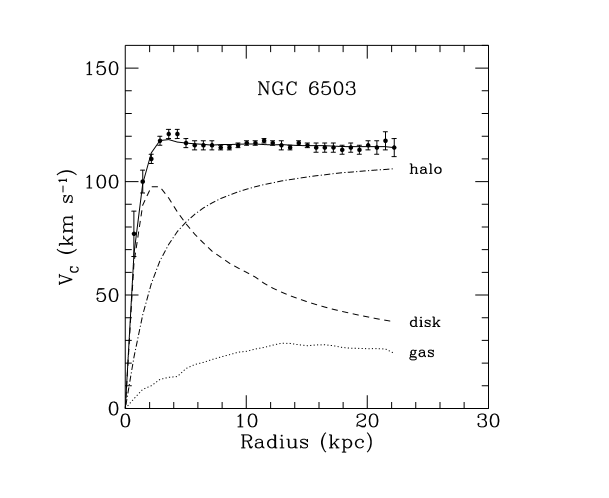
\includegraphics[scale=1.0]{Figures/DarkMatterEvidence/NGC_6503_galaxy_speed.png}
    \caption[Galaxy rotation curve for the NGC 6503 galaxy]{Galaxy rotation curve for the NGC 6503 galaxy along with different mass distribution models which together produce the fit on the observed data. The measurements are from 1991. Figure adapted from \cite{NGC_6503_galaxy_rotation_ref}}
    \label{fig:DM_Evidence_NGC_6503}
\end{figure}
These measurements have been performed multiple times and redone with modern measurements, but always producing results inconsistent with the majority of the mass being in the luminous disc.
Instead, what is suggested is that there is an invisible halo which has a mass density following $\rho(r) \propto \frac{1}{r^2}$ at large $r$.
This remains a topic on ongoing research which now focuses on Low Surface Brightness galaxies, where dark matter is the dominating component \cite{MHONGOOSE_2018_ref}.


\subsection{Galaxy Cluster Scale}
\par
At a larger scale, the discrepancy between the luminous mass and the inferred mass becomes even more apparent.
The general theory of relativity tells us that space-time is warped by the presence of mass.
As such, light propagating along null-geodesics will curve when near any object with mass, with the degree of curving being directly correlated to the intervening objects mass.
This effect, known as gravitational lensing, can be categorised as strong, weak or microlening\footnote{Strong lensing typically produces multiple images of the same object. Weak lensing has no noticeable distortion but can be discovered by statistically. Microlensing is when a significantly smaller object produces a distortion.}. 
Gravitational lensing manifests itself in observations as duplicate features and distortions.
An example of strong lensing is where light from a distant galaxy has been distorted into an arc due to the mass of an intervening galaxy, once such example is in \autoref{fig:DM_Evidence_Einstein_Ring}  where a near-perfect ring is observed.
A complete catalogue of these can be found in \cite{einstein_ring_discovery_ref}.

\begin{figure}[!htbp]%
    \centering
    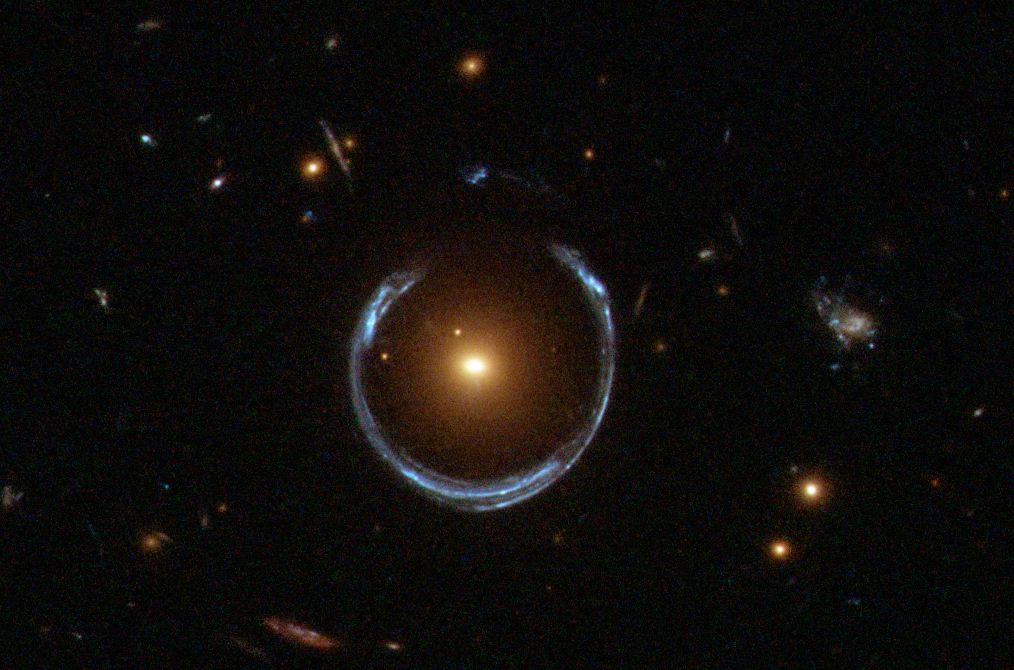
\includegraphics[scale=0.4]{Figures/DarkMatterEvidence/Einstein_Ring_from_Hubble.JPG}
    \caption{An example of a "Horseshoe Einstein Ring" created by the bending of light from a distant blue galaxy by the central red galaxy LRG 3-757 [ESA/Hubble]}
    \label{fig:DM_Evidence_Einstein_Ring}
\end{figure}

\par
Based on the amount of distortion, the mass of the object causing the lensing can be measured and can be applied to both individual galaxies as well as clusters.
The mass required for the lensing observed can then be compared to the luminous mass, which also shows a mismatch between the two \cite{History_Of_Dark_Matter_2018_ref}.


\par
At the galactic cluster scale there is the yet more evidence of the missing mass, which we'll now show for the galactic cluster 1E0657-558, also known as the Bullet Cluster.
This galaxy cluster was formed by the merger of two smaller clusters \cite{bullet_cluster_ref}.
In the resultant Bullet Cluster the baryonic matter can be tracked via electromagnetic radiation and the mass via lensing.
Observations show that there is a discrepancy between the centre of mass and the observed centre of mass, shown in \autoref{fig:DM_Evidence_Bullet_Cluster}.
The luminous matter from each of the smaller clusters mixed, causing the matter to slow down.
On the other hand, the majority of the mass has passed through.
What this indicates is that in addition to there being a significant invisible mass, this mass must also have a very small cross-section with baryonic matter and itself.

\begin{figure}[!htbp]%
    \centering
     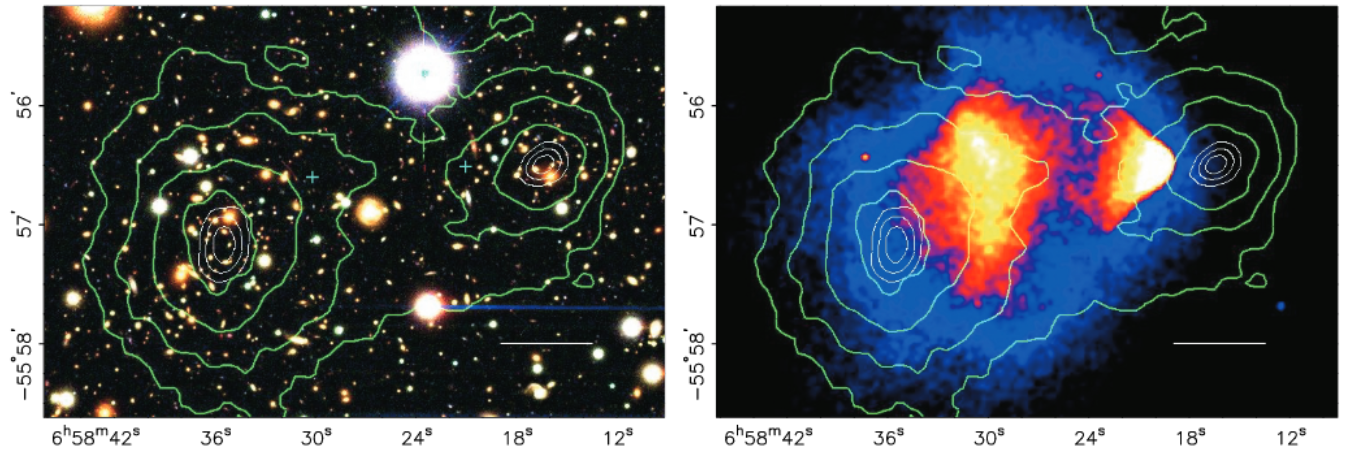
\includegraphics[width=\textwidth]{Figures/DarkMatterEvidence/bullet_cluster_2.png}
    \caption[Merging of two galaxy cluster, 1E 0657-558]{Merging of two galaxy clusters: The Bullet Cluster, 1E 0657-558.
             During the collision, the dark matter components passed through without interacting.
             The baryonic components from the two clusters interacted, causing them to lag behind .
             \textbf{Left:} Optical image from the Magellan observatory.
             \textbf{Right:} X-ray image from the Chandra observatory.
             In both figures the white bar indicates 200 kpc, the green contours are the mass distribution from weak-lensing reconstructions and the white contours are the errors on the position of the lensing peaks.
             Figure adapted from \cite{bullet_cluster_ref}.}
    \label{fig:DM_Evidence_Bullet_Cluster}
\end{figure}


\subsection{Cosmological Scale}
\par


\par
What is often quoted as the strongest evidence for dark matter comes from the cosmic microwave background (CMB) radiation which was first discovered in 1965 \cite{cmb_origins_ref}.
This is a near perfectly uniform field of microwave photons with the energy spectrum of a 2.7225 K blackbody, shown in \autoref{fig:DM_Evidence_CMB_Map}.
These photons, sometimes referred to as `relic' radiation, last interacted with with the early universe, when the temperature was almost 3000 K \cite{bigbang_nucleosynthesis_ref}.
This was some 380,000 years after the Big Bang\footnote{The surface of last scattering}, before the universe cooled sufficiently for recombination\footnote{When electrons were first able to bind to nuclei} and neutral Hydrogen formation.
At this time, the universe was filled with a plasma as there was enough energy to ionise an atom as soon as it has been formed.
The CMB photons decoupled from the plasma during this time and was able to were able to free-stream through the universe.
As the universe has expanded, these photons have red-shifted down to the now observed microwave photons, and give an insight into the early universe \footnote{It has also been quoted as ``a selfie of the baby universe" \cite{marisarthurs_thesis_ref}}.

\begin{figure}[!htbp]%
    \centering
    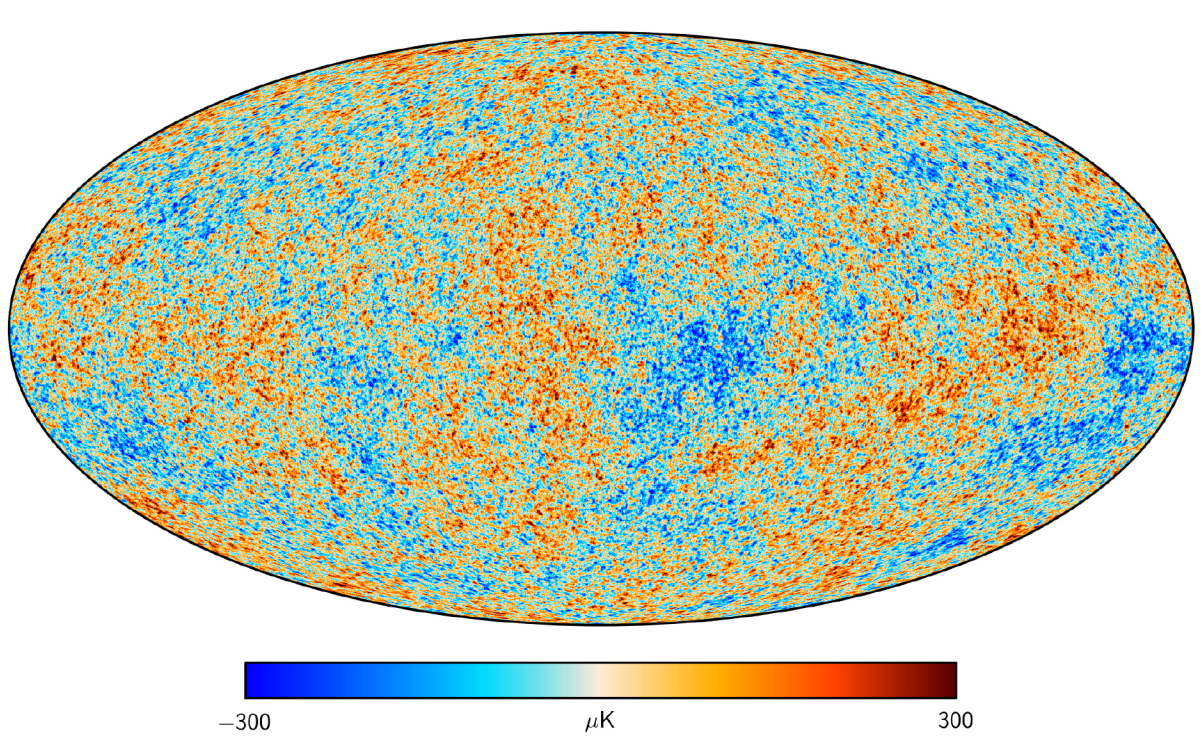
\includegraphics[width=0.8\textwidth]{Figures/DarkMatterEvidence/cmb_radiation.png}
    \caption[Temperature fluctuations of the CMB radiation]{Temperature fluctuations of the CMB radiation from Planck.
             The maximum difference between the warmest (red) and coldest (blue) is 0.0006K.
             Figure from \cite{plank_result_ref}.}
    \label{fig:DM_Evidence_CMB_Map}
\end{figure}

\par
At the time when the CMB decoupled the universe was extremely isotropic, which can be seen in the uniformity of the CMB, though there are minor anisotropies.
Prior to recombination, any small non-uniformity in the plasma resulted in a gravitation well, into which all forms of matter were pulled into.
The inward force of gravity competed with the outward force from photons, tied with the expanding (and therefore cooling) universe resulted in standing pressure waves in the plasma, referred to as baryon acoustic oscillations (BAO), and describe the temperature fluctuations.
Describing them as spherical harmonics ($Y_{lm}(\theta,\phi)$, the temperature fluctuations can be written as \cite{History_Of_Dark_Matter_2018_ref}:
\begin{equation}
    \frac{\delta T}{T}(\theta, \phi) = \sum_{l} \sum_{m} a_{lm}Y_{lm}(\theta,\phi)
    \label{eq:bao_spherical_harmonics}
\end{equation}
The temperature fluctuations between two points in the CMB can then be described by:
\begin{equation}
    C(\theta) = \frac{1}{4\pi} \sum_{l} (2l + 1) C_l P_l (cos(\theta))
\end{equation}
where $\theta$ is the angular separation between two points and $P_l (cos(\theta))$ are Legendre polynomials.
$C_l$ can be considered as the magnitude of the temperature fluctuation when $l$ is large, making $l$ analogous to $\theta$.
The application of this on the lasted Planck result is shown in \autoref{fig:DM_Evidence_BAO} \cite{plank_result_ref}.
\begin{figure}[!htbp]%
    \centering
    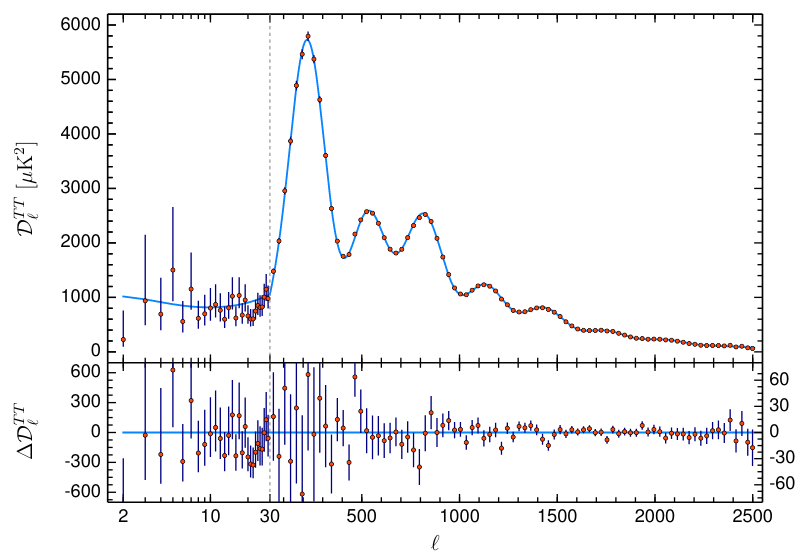
\includegraphics[width=0.8\textwidth]{Figures/DarkMatterEvidence/bao.png}
    \caption[Temperature fluctuations of the CMB spectrum as a function of $l$]{The temperature fluctuations of the CMB power spectrum against the spherical harmonics multipole parameter, $l$, which is a proxy for angular separation.
             \textbf{Top:} the power spectrum fitted to the $\Lambda$CDM model.
             \textbf{Bottom:} the residuals of the fit, shown to be small.
             Figure from \cite{plank_result_ref}.}
    \label{fig:DM_Evidence_BAO}
\end{figure}
\par
The shape of the spectrum in \autoref{fig:DM_Evidence_BAO} sets significant constraints on the $\lambda$CDM model, with the latest Planck result, the observed CMB is best fitted with a energy density in the universe divided up as: 4.88\%$\pm$0.03\% baryonic matter, 26.01\%$\pm$0.22\% and the remaining 69.11\%$\pm$0.62\% being dark matter \cite{plank_result_ref}.

\section{Candidates}
\par
With there being a plethora of evidence that "something is there", we can turn our attention to what it might be.
From the observation, we can say that an potential candidate for dark matter must be;
\begin{itemize}
    \item Weakly, or not interacting via electromagnetism 
    \item Weakly, or not interacting via the strong force
    \item Have some kind of clustering; either by being slow moving (cold) or some other way
    \item Not baryonic matter
    \item Stable over the timescale of the Universe.
\end{itemize}
Additionally, it may be beneficial to start with the Standard Model of particle physics, and look for extensions which satisfy the above requirements.
In this section a brief description of proposed candidates are described briefly, followed by possible the most favoured candidate; the weakly interacting massive particle (WIMP)
It should be noted that many of these particles.

\subsection{MACHOs and primordial black holes}
\par
The first set of candidates seems like a very good candidate on the surface.
Massive astrophysical compact halo objects (MACHOs) are objects such as star remnants, very faint stars and 
and primordial black holes are non-luminous.
These have been some of the earliest possible explanations and have been favourable as they don't require new matter.

\par
Microlening surveys are able to observe objects with XYZ properties, but are limited to XYZ masses.
If such 
Unfortunately microlening searching have shown that MACHOs cannot make up more than 25\% of galactic halo masses.

\par
Black holes are also a contributor. 
These are a favoured solution as well as they are comprised of understood matter, and will the LIGO collaboration having measuring the merger of black holes, and the first image of a black hole being taken in XXX, our understanding of them as a component is increasing.
However, black holes such as that at the centre of the Milky Way are not believed to have been around in the minutes after the Big Bang but rather from the collapsing of some of the earliest super massive stars.
Instead, primordial black holes must have existed, formed from a different process in the early minutes after the Big Bang.
This is supported by some of the measurements from LIGO such as the merger of black holes of around 30 solar masses.
A black hole of this mass is not as likely to be produced from the regular stellar evolution.
Assuming that there are indeed primordial black holes, then they would contribute at least in part to dark matter.
If these primordial black holes were to be the dominant explanation for dark matter, then the model for the formation of the early universe needs addressing.
Our understanding on this topic is still evolving and the amount that this contributes to dark matter will be pinned down.

\subsection{Modified Gravity}
\par

\subsection{Neutrinos}
\par
One of the first candidates suggested as dark matter were neutrinos: the stable, long-lived and weakly-interacting particles in the standard model.
Unfortunately, N-body simulations shown that given the relativistic velocities are inconsistent with the structural formations that we observe \cite{neutrinos_and_galaxy_clustering_ref}. 
This has not ruled out neutrinos entirely, with a new species suggested which interacts only gravitational \cite{sterile_neutrinos_ref}.
Postulated to have a small mixing angle with standard model neutrinos, this would allow for limited interaction between this dark matter and SM matter.
\par
The most recent excitement around this is an unidentified 3.55keV line in X-ray spectra from several galactic clusters with high dark matter content \cite{sterile_neutrino_xray_decay_ref}, with one possible interpretation is the decay of sterile neutrinos, though there is much debate around this \cite{xray_from_sterile_neutrons_2_ref, xray_from_sterile_neutrons_3_ref}.
Separately, results by MicroBooNE have indicated neutrino mixing that is inline with the standard model, going against previous results from MiniBooNE where an excess in neutrino oscillations \cite{miniboone_and_microboone_sterile_neutrino_ref}.
The BEST experiment has also pointed towards sterile neutrinos to account for the deficit observed in germanium isotope production \cite{best_sterile_neutrino_result_ref,best_sterile_neutrino_2_ref}.
With the correct properties, the sterile neutron could contribute to dark matter, though as the understanding of the neutrinos we already know about contains significant gaps (such as the mass hierarchy), more work is needed \cite{sterile_neutrino_as_dm_ref, sterile_neutrinos_dm_ref}.

\subsection{Axions}
\par
Hypothesised in 1977, axions were postulated to solve the strong CP problem of the standard model \cite{axion_origins_ref}.
Axions are a pseudo-Goldstone boson generated by spontaneous symmetry breaking at some energy scale, $f_a$, with the mass of this particle predicted to follow:
\begin{equation}
    m_a \approx (0.6eV)\frac{10^7 GeV}{f_a}
\end{equation}
The value of $f_a$ is constrained to be greater than that of the electroweak symmetry-breaking scale, given exciting constraints on experiments.
This leaves a particle with a mass between 10${}^{-6}$ and 10${}^{-2}$eV for which they could account for dark matter \cite{axions_ref}.
\par
There are multiple proposed production mechanisms for axions such as via thermal production in the early universe.
However, axions produced in this fashion would contribute to hot dark matter the constraints are very limitting \cite{hot_axions_ref}.
Separately, slower, non-relativistic axions can be created through other processes such as "re-alignment mechanism" \cite{cold_axion_ref}.
\par
Axions may couple to photons, allowing for a conversion to microwaves.
These can be searched for in a microwave cavity with a strong magnetic field applied to it.
In this situation it is expected that the axion will convert into monochromatic microwave photons.
The ADMX experiment has adopted this approach and is currently the most sensitive experiment to this \cite{admx_experiment_ref}.
\par
Another search of axions is where an axion is absorbed and an atomic electron is ejected.
This electron is then detectable as an electronic recoil.
These searches are typically performed by large underground direct dark matter experiments, with the tightest constraint on axio-electric coupling coming from XENONnT \cite{xenonnt_sr1_er_ref}.
\par
A third approach is via laser beams whereby a beam is propagated between two superconduction magnets that are optically separated.
If axions are coupling to photons, then the initial beam will transform into an axion and then later convert back, allowing the light to be seen through the optical barrier.
Though not as sensitive as the other axion-photon conversion approaches, it does not have the same uncertainties associated with astrophysics and cosmology.
Two notable experiments using this approach are ALPS \cite{alps_axion_result_ref} and OSQAR \cite{osqar_axion_result_ref}. 
\par
Other search methods are also being explored such as axion induced nuclear electric dipole moment (see CASPEr \cite{casper_experiment_ref}), axion to X-ray conversion in the presence of a magnetic field (see IAXO \cite{iaxo_experiment_ref}), and energy-loss in galactic observables such as supernova explosions due to axion-electron coupling \cite{axions_from_supernova_ref}.

\subsection{WIMPS}
\label{sec:wimp_as_a_candidate}
\par
Another candidate, are arguably the most popular is a set of new particles that interact via the weak force, but have a lot of mass.
Namely, Weakly Interacting Massive Particles (WIMPs)\footnote{this differs from the original meaning where the interaction probability was low}. 
\par
In this case, dark matter is formed of stable particles from the early universe.
At this time, WIMPs were in thermal equilibrium with the rest of the universe: so the self-annihilation rate was equal to that of the creation rate from interactions between light particles.
As the universe expanded, the density of WIMPs decreased until the self-annihilation rate dropped.
Referred to as "thermal freeze-out", the remaining WIMPs appear as a relic abundance. 




\par
Known as the "WIMP miracle", this connection between cosmology and particle physics has helped give WIMPs the prevalence it has.


\par
Additionally, there are certain extensions to the standard model which are able to solve problems including the hierarchy problem and gauge coupling unification which also produce a WIMP candidate.


\par
In addition to supyersymmetry, WIMP-like dark matter particles do appear from other theories.
The typical search strategy for WIMPs by large underground detectors such as LUX-ZEPLIN \cite{LZ_TechnicalDesignReview_ref}, XENONnT \cite{xenonnt_projected_sensitivty_ref} and PandaX-4T \cite{pandax_4t_ref}.

\section{Dark Matter Searches}
\par
Maybe have this as a separate chapter? And go into more detail about signals?

\par
There are generally speaking, three routes of detection can be classified as;

\begin{itemize}
    \item Production
    \item Indirect
    \item Direct
\end{itemize}
    
    

\subsection{Direct Detection}

\subsection{Indirect Detection}

\subsection{Production}
\par
In some experiments it may be possible to produce dark matter.
In particle colliders such as the Large Hadron Collider (LHC) this process may occur.
The act of smashing together protons and observing the jets output.
This may occur in proton-proton collisions: $pp\xrightarrow{}\chi\chi$.

\par
When two protons are collided together, what is observed are a bunch of jets. 
But we don't care about that... Down with the LHC!

\par
The primary observable applicable to a dark matter search is the missing momentum.
A search may be performed by searching for an excess of this missing energy when compared to the Standard Model background.





\par
Though these experiments may not be able to fully characterise dark matter, they do offer the best way for discovering new invisible particles.
However, they are hindered as any dark matter particle mass to be approximately 50\% of the mediator mass.
Though this is complimented by what direct detection offers with the sensitivity limited by the neutrino
\par
The LHC, at the time of writing, is undergoing an upgrade ahead of a planned 14 TeV centre-of-mass energy science run. 
This High-Luminosity run, due to begin data-taking in 2026 will allow for improved searches into dark matter.



%\chapter{Direct Detection of WIMPs}
\label{chap:detection_theory}
\par
We have seen in the previous chapter that there is a wealth of evidence for some particle or particle combination that is missing from our understanding of particle physics.
In this Chapter, we focus on WIMPs that were introduced in \autoref{sec:wimp_as_a_candidate}, and how they may interact with nucleons in a way that can be detected by Earth based detectors.


\section{WIMP-nucleon interactions} \label{sec:wimp_nucleus_interactions}
\iffalse
\par
As WIMPs travel at relative non-relativistic speeds, the recoil energy of the nucleon resulting from an elastic scatter is by only the centre of mass scattering angle, $\theta$ \cite{direct_detection_of_wimps_ref}:
\begin{equation}
    E_{R} = \frac{{\mu}_{N}^{2}\nu_{\chi}^2}{m_{N}}(1-\cos(\theta))
\end{equation}
\fi
Direct dark matter detectors are built on the principle of having a large mass of material on which a WIMP can scatter \cite{direct_detection_of_wimps_ref}.
Within a detector, the rate of these WIMP scatter interactions, $R$, is given by:
\begin{equation}
    R = \sigma N_{T} n_{\chi} \langle v \rangle
    \label{eq:wimp_nucleon_rate}
\end{equation}
where N$_{T}$ is the number of nuclei in the detector, $n_\chi$ is the number density of dark matter particles travelling with an average speed $\langle v \rangle$ relative to the target, and $\sigma$ is the interaction cross-section, representing the interaction strength between the dark matter and the nucleus.
\par
Given that each direct detector is sensitive to different recoil energies depending upon the design, it is beneficial to describe the event rate in an energy region as the differential scattering rate with respect to recoil energy \cite{supersymetry_wimpy_boi_ref}:
\begin{equation}
\begin{split}
    \frac{dR}{dE_R} &= \frac{\rho_{\chi}}{m_\chi m_A} \int^{\infty}_{v_{min}} v f(\vec{v}) \frac{d\sigma}{dE_R} d\vec{v} \\
                    &= \frac{2\rho_{\chi}}{m_\chi} \int^{\infty}_{v_{min}} v f(\vec{v}) \frac{d\sigma}{d |q|^2} d\vec{v}
\end{split}
\label{eq:wimp_differential_rate}
\end{equation}
where $f(\vec{v})$ is the dark matter velocity distribution in the galactic halo, $\rho_{\chi}$ is the dark matter density, $m_\chi$ is the dark matter mass, $m_A$ is the target nucleus mass, and $q$ is the momentum transfer associated with the recoil given by $q = \sqrt{2m_A E_R}$ and $v_{min}$ is the minimum velocity of dark matter to induce a recoil of energy $E_R$.
It is therefore a detector specific limit given by $v_{min} = \sqrt{(m_\chi E_R)/(2\mu^2)}$ where $\mu = (m_\chi m_A)/(m_\chi + m_A)$, the WIMP-nucleus reduced mass.
\par
We are able to control the detector size and target properties (within reason).
This leaves us with two parameters outside of our direct control but which we need to constrain in order to determine an expected rate in any given detector: the dark matter velocity distribution and the differential cross-section.

\subsection{Local Astrophysical Dark Matter Properties}
\par
The standard dark matter model has two parameters that need to be determined experimentally: the velocity distribution and the density. 
Both have sufficient uncertainties to significantly impact the sensitivity of any direct detection experiment \cite{local_dm_uncertainties_ref}.
\par
The local dark matter density has long been studied, with the earliest references from 1922 \cite{first_dm_density_1_ref, first_dm_density_2_ref}.
Since then, many measurements have been done which constrain $\rho_{\chi}$.
These fall into two categories: galactic measurements and local measurements \cite{dm_density_ref}.
Galactic measurements derive $\rho_{\chi}$ from rotation curves, which does not require the assumption of a galactic halo.
Local measurements typically observe tracer star motion near the Sun \cite{gaia_tracer_dm_density_ref}.
Naturally there is variation in these two approaches where the galactic measures place $\rho_{\chi}$ in the range 0.2-0.6 GeV/cm$^3$ whilst the latest result from Gaia \cite{gaia_data_2_ref} have $\rho_{\chi}$ between 0.1-1.5 GeV/cm$^3$ \cite{gaia_dm_density_2_ref}.
Prior to the second data release of Gaia, the best-fit of all the studies lay in the range 0.22-0.33 GeV/cm$^3$, as such $\rho_{\chi}$ has typically been taken to be 0.3 GeV/cm$^3$.
This may change in the coming years as the current best-fit from Gaia studies suggest $\rho_{\chi}=0.5$ GeV/cm$^{3}$ \cite{gaia_dm_density_1_ref}.
\par
With regard to the velocity distribution, there are a number of models that are often used. 
Including simple isotropic models \cite{isotropic_dark_matter_models_ref}, isothermal sphere dark matter \cite{dm_velocity_isothermal_ref} and the Standard Halo Model (SHM) \cite{dm_velocity_shm_ref}. 
We shall only consider the SHM here as it is the most common choice \cite{dark_matter_distribution_models_ref}.
\par
In the SHM, a Maxwell-Boltzmann velocity distribution is assumed, which is truncated at the escape velocity ($v_{\text{esc}}$) of the Milky Way \cite{direct_dark_matter_of_wimps_concepts_ref}.
This constrains the dark matter to be within the galaxy.
The SHM also assumes dark matter is isotropic and spherically symmetrically distributed in the galaxy\footnote{The distribution is not perfectly symmetrical, and there are newer models referred to as SHM$^{++}$ which try and account for this, but they are not considered here \cite{extended_shm_ref}}.
The velocity distribution of dark matter within the Milky Way halo in the Earth frame is approximated as \cite{direct_dark_matter_of_wimps_concepts_ref, shm_derivation_ref}:
\begin{equation}
    f(\vec{v}) = \frac{1}{k} e^{\frac{- (\vec{v} - \vec{v}_E)^2 }{ v^2_0} }
    \label{eq:shm_short_equation}
\end{equation}
where $\vec{v}$ is the velocity of the dark matter with respect to the Earth, $\vec{v}_E$ is the velocity of the Earth around the centre of the galaxy and $\vec{v}_0$ is the peculiar velocity of the Sun relative to its circular velocity. 
\autoref{eq:shm_short_equation} is only valid for when $|\vec{v} + \vec{v}_E| < v_{\text{esc}}$.


%\begin{equation}
% f(\vec{v}) = \frac{1}{(2\pi\sigma^2_{v})^{\frac{3}{2}}N_{esc}} e^{\frac{- |\vec{v}|^2}{2\sigma^2_v}} \Theta(v_{esc} - |\vec{v}|)
%\label{eq:shm_velocity_1}
%\end{equation}
%where $\Theta$ is a Heaviside step function, $\sigma_v$ is the velocity dispersion, and .
%
%\par
%The dark matter velocity distribution which was used in \autoref{eq:wimp_differential_rate_scattering_amplitude} was normalised such that $\int f(\vec{v}) dv = 1$.
%As such we need to renormalise \autoref{eq:shm_velocity_1} to allow for the integral of $\sigma_{v}$ to be unitary as well.
%We do this by:
%\begin{equation}
%    N_{esc} = erf(z) - 2z e^\frac{-z^2}{\pi^{\frac{1}{2}}}
%\end{equation}
%where erf is the error function (given by $\text{erf}(z) = 2/\sqrt{\pi}\int^{z}_{0} e^{-t^2} dt$) and $z=v_{esc}/v_0$.
%We also need to define two other variables: $x=v_{min}/v_{0}$ and $y=|V_E|/v_0$ where $|V_E|$ is the velocity of the Earth with respect to the dark matter halo.
%Using these we can define our integral as \cite{shm_derivation_ref}:
%\begin{equation}
%\begin{split}
% \int \frac{f(\vec{v})}{v} = 
%\begin{dcases}
%\frac{1}{v_0 y}  & \text{if}\; z<y,x<|y-z| \\
%\frac{1}{2N_{esc} v_{0}y} \bigg[\text{erf}(x+y) - \text{erf}(x-y) - \frac{4}{\sqrt{\pi}}ye^{-z^2} \bigg] & \text{if}\; z>y, x<|y-z| \\
%\frac{1}{2N_{esc} v_{0}y} \bigg[\text{erf}(z) - \text{erf}(x-y) - \frac{2}{\sqrt{\pi}}(y + z - x)e^{-z^2} \bigg] & \text{if}\; |y-z|<x<|y+z|
%\end{dcases}
%\end{split}
%\label{eq:shm_velocity_2}
%\end{equation}
\par
Depending upon the values used for both the dark matter density and the velocities, the scattering rate will vary, and therefore the sensitivity of any given experiment will vary.
Historically the parameters used for determining the event rate have varied between experiments, making comparisons between results difficult.
However, recent collaboration between dark matter experiments have now agreed upon a common set of parameters \cite{standard_halo_model_conventions_ref} summarised in \autoref{tab:standard_parameters_for_dm}.
For a review of how these affect sensitivity to a dark matter discovery, the reader is directed to \cite{dm_velocity_effects_on_limits_ref}.

\begin{table}[]
    \centering
    \begin{tabular}{c|c|c}
        Parameter                               & Description                       & Value         \\ \hline
        $\rho_{\chi}$                           & Local dark matter density         & 0.3 GeV/cm$^2$ \cite{shm_derivation_ref}           \\
        $v_{esc}$                             & Galactic escape velocity          & 544 km/s  \cite{dm_v_esc_ref}           \\
        $v_0$                             & Local standard of rest velocity   & 238 km/s   \cite{dm_v_0_ref}           
    \end{tabular}
    \caption{Suggested Standard Halo Model parameters adapted from \cite{standard_halo_model_conventions_ref}}
    \label{tab:standard_parameters_for_dm}
\end{table}

\subsection{Differential cross-section}
%\par
%In order to allow for comparisons between experiments with different target nuclei, it is typical to convert from a WIMP-nucleus cross-section ($\sigma_A$) to a WIMP-nucleon cross-section ($\sigma_N$).
In the zero-momentum transfer regime, the WIMP-nucleus cross-section can be expressed as:
\begin{equation}
    \frac{d\sigma}{d|q|^2} = \frac{\sigma_0}{4\mu^2 v^2} F^2(q)
\end{equation}
where $\sigma_0$ is the total cross-section at zero-momentum transfer and $F(q)$ is the nuclear form factor that encapsulates the momentum dependence of the cross-section \cite{shaunalsum_thesis_ref}.
This identity is known as Fermi's Golden rule \cite{shaunalsum_thesis_ref}.
\par
As has already been said, we are constraining ourselves to non-relativistic scattering.
Therefore only interactions which do not vanish in the zero-momentum transfer limit are considered.
In this zero-momentum transfer limit, there are two forms of interactions: a spin-independent (SI) and a spin-dependent (SD) component  \cite{wimp_lagrangian_ref}.
Therefore the differential cross-section is actually given by:
\begin{equation}
    \frac{d\sigma}{d|q|^2} = \bigg(\frac{d\sigma}{d|q|^2}\bigg)_{SI} + \bigg(\frac{d\sigma}{d|q|^2}\bigg)_{SD}
\end{equation}
The SI interaction arises from the WIMP coupling to quarks mediated via a Higgs, whereas SD interactions arise from the axial-vector interaction between WIMPs and quarks \cite{supersymmetric_dark_matter_ref}.
As the weighted contributions of the SI and SD components are not known and to make experimentalists lives easier, each interaction is generally considered independently, but for those interested in mixing these terms, the interaction Lagrangian can be found in \cite{wimp_lagrangian_ref}.
%, following \cite{supersymetry_wimpy_again_ref}.
\par
Taking the SI case only, and so setting the contribution from SD to zero, the dimensionless constant $C$ is:
\begin{equation}
    \sigma_0 = \frac{4\mu^2}{\pi} [f_pZ + f_n (A-Z)]^2
\end{equation}
where $A$ and $Z$ are the atomic mass and atomic number respectively.
$f_n$ and $f_p$ are the dark matter couplings to neutrons and protons.
\par
If we assume that the coupling for WIMPs to protons and neutrons is similar\footnote{so isospin is conserved} ($f_p \backsim f_n$) then the relation between the WIMP-nucleus and WIMP-nucleon cross-sections is given by:
\begin{equation}
    \sigma_{0} = \frac{\mu^2}{\mu^2_n}A^2 \sigma_{n}
\end{equation}
where $\mu_n$ is the WIMP-nucleon reduced mass and $\sigma_n$ is the WIMP0nucleons cross-section.
\par
The final WIMP-nucleon elastic scattering differential rate for an SI interaction is then given by:
\begin{equation}
    \frac{dR}{dE_R} = \frac{\rho_\chi}{2 m_\chi \mu^2} F^2(q) \int^{\infty}_{v_{min}} \frac{f(\vec{v})}{v} A^2 \sigma_{0N} d\vec{v}
    \label{eq:wimp_si_differential_rate}
\end{equation}
An equivalent derivation for SD interactions can be found in \cite{wimp_theory_ref}.
It is typical to report any result in terms of WIMP-nucleon cross-section as it removes the dependence on the target nuclei, allowing different experiments to compare results easily.

\par
In the left plot of \autoref{fig:si_recoil_and_form_factor}, the differential event rate for a selection of frequently used targets is shown.
In \autoref{fig:si_recoil_and_form_factor}, a WIMP mass of 100 GeV/c$^2$ is used with a WIMP-nucleon cross-section of 10$^{-45}$ cm$^2$ (i.e. 1 zb).
Results from experiments are typically normalised to a cross-section of 1 zb to allow for easier comparison.
The heavy target nuclei have a larger event rate for low-energy nuclear recoils.
This is due to the A$^2$ enhancement seen in \autoref{eq:wimp_si_differential_rate}.
A lower scattering rate is seen for lighter nuclei, but at higher recoil energies, they have a higher rate than heavy nuclei.
This is due to a rate suppression by the form factors (discussed in the next section) and a decrease in kinematically-allowed WIMP velocities with an increase in $m_A$ and $E_R$.

\begin{figure}
    \centering
    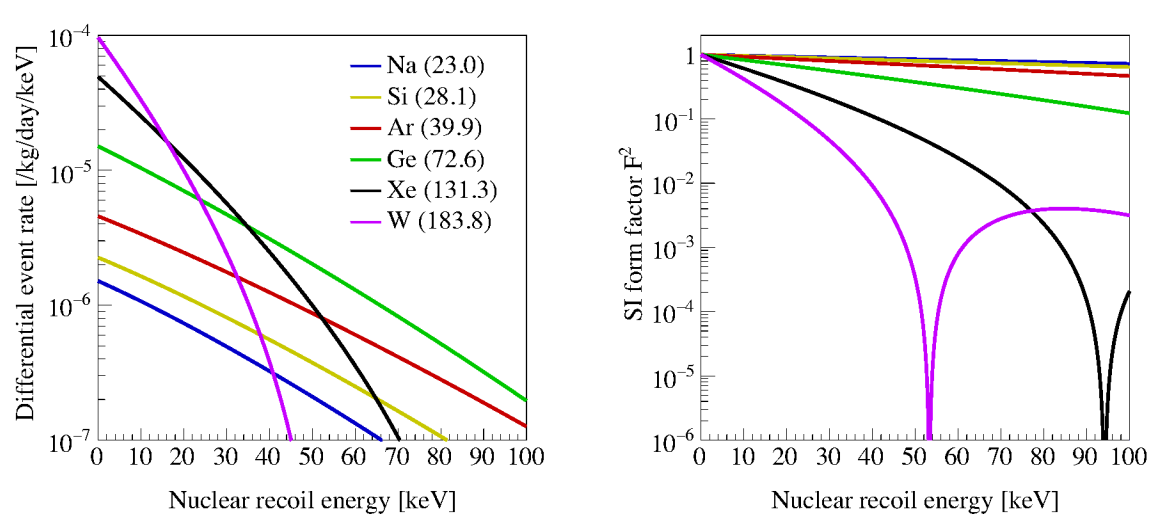
\includegraphics[width=\textwidth]{Figures/LZ/SI_recoil_rate_and_spectra.png}
    \caption{\textbf{Left:} SI nuclear recoil rate for a selection of target elements for a WIMP mass of 100 GeV/c$^2$ and WIMP-nucleon corss section of $\sigma_N=$1 zb and the recommended parameters for the SHM. The averaged atomic mass of each target from natural abundance is in the brackets.
    \textbf{Right:} The Helm form factors for a selection of target nuclei. The key is the same in both plots.
    Both plots are from \cite{LZ_Ibles_LZStats_Thesis_ref}
    \label{fig:si_recoil_and_form_factor}.
           }
\end{figure}
 
\subsection{Form Factors}
\label{sec:form_factors}
\par
One feature which hasn't been mentioned in detail yet is the form factor, $F(q)$.
The form factor contains the physics of the nucleus and is the Fourier transform of the density distribution within.
For SI interactions, this is taken to be the Helm form factor where the nucleus is represented as a solid sphere of radius $r_n$, with a smooth density of nucleons described by a Gaussian of thickness $s$ \cite{helm_form_factor_ref}:
\begin{equation}
    F^2(q) = \bigg( \frac{3j_i(qr_n)}{qr_n} \bigg)^2 e^{-q^2 s^2}
\end{equation}
where $j_i$ is the Bessel function.
\par
%As $r_n \backsim A^{1/3}$ fm, we can see that the WIMP cannot resolve the nucleus as a point-like object.
In the right plot of \autoref{fig:si_recoil_and_form_factor}, the Helm form factors for a selection of popular targets are shown.

\par
For SD interactions, the coupling is not equal between protons and neutrons and so the choice of which nucleus description to use is fairly important.
Depending on which is used the resultant sensitivity to dark matter can vary by orders of magnitude \cite{wimp_nuclear_model_ref,wimp_sd_form_factor_ref}.


\section{Effective Field Theory} \label{sec:eft_theory}

\par
Given the now decades of searching for SI and SD interactions with no success it is right to ask if the assumptions made there are still best.
There may be other corrections (such as momentum dependence) that are the dominant terms.
It is therefore useful to approach a direct dark matter search in a model independent way - namely via an effective field theory (EFT).
\par
An EFT is allows us to describe an unknown model to an arbitrary accuracy by only described the physics at a given scale \cite{eft_expo_ref}.
We parameterise our model in terms of whatever we like though could be in terms of quantities such as energy, momentum or velocity\footnote{This has rather elegantly been quoted as a way to ``parameterise our ignorance" in \cite{shaunalsum_thesis_ref}}.

\par
In the remainder of this chapter we explore the elastic scattering rates in within this model independent approach.
The broad framework which we will follow is from \cite{Fitzpatrick_2013_ref}.

\subsection{Possible Operators}

\par
We begin our journey by treading the WIMP-nucleon elastic scattering as a four-field interaction comprising of the WIMP field $\chi$, the nucleon field $N$ and the effective operators $\Operator$:
\begin{align}
\begin{split}
    \Lagrangian_{int} &= \chi^{+} \Operator_{\chi} \chi^{-} N^{+} \Operator_{N} N^{-} \\
                      &= \Operator \chi^{+}\chi^{-} N^{+}N^{-}
\end{split}
\label{eq:eft_initial_lagrangian}
\end{align}
Now, we can impose constraints by applying symmetries.
\par
Firstly, any operator must be invariant with respect to constant shift in velocities: Galilean invariant.
This allows gives us four quantities with Galilean invariance: momentum transfer, $\vec{q} = \vec{p}_{\chi 1} - \vec{p}_{\chi 2} = \vec{p}_{N 2} - \vec{p}_{N 1}$, the incident WIMP velocity, $\vec{v}=\vec{v_\chi} - \vec{v}_N$, and the spins of the particles: $\vec{S}_N$ and $\vec{S}_\chi$.

\par
Next we look at energy conservation in the centre of mass frame as it cannot change in the collision.

This allows us to equate the initial energy, $E$:
\begin{align}
    E  = \frac{1}{2}\mu_N v^2
\end{align}
to the final kinetic energy, $E'$:
\begin{align}
\begin{split}
    E' &= \frac{1}{2}\mu_N v'^2 \\
       &= \frac{1}{2}\mu_N (\vec{v} + \frac{\vec{q}}{\mu_N})
\end{split}
\end{align}
where $\mu_N=(m_\chi m_N)/(m_\chi + m_N)$ is the WIMP-nucleon reduced mass.
This leaves us with:
\begin{equation}
    \vec{v}\vec{q} = \frac{q^2}{2\mu_N}
\end{equation}
Finally we want the operators to be real values, corresponding to physical quantities, that is to say, Hermitian.
Neither $\vec{q}$ nor $\vec{v}$ are Hermitian, but can be made so by:
\begin{equation}
\begin{split}
    &\vec{q} \rightarrow i\vec{q} \\
    &\vec{v} \rightarrow \vec{v}^{\bot} = \vec{v} + \frac{\vec{q}}{\mu_N}
\end{split}
\end{equation}
There four quantities make up the complete set of parameters which we need to describe our interaction.
We can then take all of the combinations of these variables to leave us with 15 operators:
\begin{equation}
\begin{array}{lcl}
\Operator_{1}=1_{\chi}1_N, \quad \Operator_{2}=\left(v^{\perp}\right)^{2}, \quad \Operator_{3}=i \vec{S}_{N} \cdot\left(\frac{\vec{q}}{m_N} \times \vec{v}^{\perp}\right) \\ 
\Operator_{4}=\vec{S}_{\chi} \cdot \vec{S}_{N}, \quad \Operator_{5}=i \vec{S}_{\chi} \cdot(\frac{\vec{q}}{m_N} \times \vec{v}^{\perp}) \\ 
\Operator_{6}=\left(\vec{S}_{\chi} \cdot \frac{\vec{q}}{m_N}\right)\left(\vec{S}_{N} \cdot \frac{\vec{q}}{m_N}\right) \\
\Operator_{7}=\vec{S}_{N} \cdot \vec{v}^{\perp}, \quad \Operator_{8}=\vec{S}_{\chi} \cdot \vec{v}^{\perp} \\
\Operator_{9}=i \vec{S}_{\chi} \cdot\left(\vec{S}_{N} \times \frac{\vec{q}}{m_N}\right), \quad \Operator_{10}=i \vec{S}_{N} \cdot \frac{\vec{q}}{m_N} \\ 
\Operator_{11}=i \vec{S}_{\chi} \cdot \frac{\vec{q}}{m_N}, \quad \Operator_{12} =\vec{S}_{\chi} \cdot\left(\vec{S}_{N} \times \vec{v}^{\perp}\right) \\
\Operator_{13} =i\left(\vec{S}_{\chi} \cdot \vec{v}^{\perp}\right)\left(\vec{S}_{N} \cdot \frac{\vec{q}}{m_N}\right) \\ 
\Operator_{14} =i\left(\vec{S}_{\chi} \cdot \frac{\vec{q}}{m_N}\right)\left(\vec{S}_{N} \cdot \vec{v}^{\perp}\right) \\ 
\Operator_{15} =-\left(\vec{S}_{\chi} \cdot \frac{\vec{q}}{m_N}\right)\left(\left(\vec{S}_{N} \times \vec{v}^{\perp}\right) \cdot \frac{\vec{q}}{m_N}\right)
\end{array}
\label{eq:EFT_Operators}
\end{equation}
$\Operator_{1}$-$\Operator_{11}$ can be attributed to the exchange of spin-0 or spin-1 mediators, where as $\Operator_{12}$-$\Operator_{15}$ do not.
Some literature also include $\Operator_{16}=-((\vec{S}_\chi \times \vec{v}^{\bot}) \cdot \vec{q})(\vec{S}_N) \cdot \vec{q})$, though as it is just a linear combination of $\Operator_{12}$ and $\Operator_{15}$ it does not need to be included for the most general description.
Typically $\Operator_{2}$ is disregarded due to the $v^{2}$ dependence and so does not appear in non-relativistic models and has such will be dropped here as well.

\par
Before we continue it is important to note that the couplings to the nucleon components are not necessarily the same as each.
This means that each operator, $\Operator$, really represents 2 operators: $\{proton,neutron\}$ or with isospin dependency $\{isoscalar,isovector\}$.
Protons and neutrons are fairly self-explanatory.
Isoscalar particles are singlets with a total isospin of 0 where as isovector particles are triplet states with a total isospin of 1.
Historically there has been limited consistence, with often the same experiment changing between $\{neutron, proton\}$ basis and $\{isoscalar, isovector\}$ basis between data runs.
The choice for some experiments to adopt the $\{neutron, proton\}$ basis has been driven by similarity in reporting results with the standard spin-dependent analysis.
In the last few years however, $\{isoscale, isovector\}$ basis has become more common, with CDMS, XENON100, DEAP-3600 and PandaX-II all reporting results in this basis \cite{cdms_eft_ref,xenon100_eft_ref,deap3600_eft_ref,pandax_2_eft_ref}.
Therefore, in any evaluation a decision needs to be made as to which approach to use.
The translation is fairly trivial with the coupling constants between isoscalar ($c^0$), isovector ($c^1$), proton ($c^p$) and neutron ($c^n$) given by:
\begin{equation}
\begin{split}
    c_i^0 &= \frac{1}{2}(c_i^p + c_i^n)  \\
    c_i^1 &= \frac{1}{2}(c_i^p - c_i^n) 
\end{split}
\label{eq:eft_iso_to_pn}
\end{equation}
In practical terms, this means that out Lagrangian (\autoref{eq:eft_initial_lagrangian}) requires a slight alteration to:
\begin{equation}
    \mathcal{L}_{int}  = \sum_{\tau = (0,1)} \sum_{i}c^{\tau}_{i} \Operator \chi_1 \chi_2 N_1 N_2
\end{equation}
for $\{isoscalar,isovector\}$ and to:
\begin{equation}
    \mathcal{L}_{int} = \sum_{N = (p,n),(\tau)} \sum_{i}c^{(N)}_{i} \Operator \chi_1 \chi_2 N_1 N_2
\end{equation}
for $\{p,n\}$, where $\tau$ refers to the isospin basis.
A priori we know nothing about the strength of these coefficients, and so we cannot say that we know one operator is more significant than another operator.

\par
Although we have constrained ourselves to elastic scatter, this theory can be trivially extended to the inelastic case by $\vec{v}^{\perp} \rightarrow \vec{v}^{\perp} + \frac{\delta_m}{|\vec{q}|^2}\vec{q}$ \cite{inelastics_eft_ref}.

\subsection{To the Nucleus}
\par
Now in order to relate the theory outlined above to what is observable experimentally we must consider that a dark matter particle interact with nucleons that are bound in nuclei rather than free nucleons.
As such, each $\Operator$ needs to be evaluated inside of the target nucleus, and so inserted between nuclear states.
In order to assist in this, we first decompose $\vec{v}$ of each nucleon into the velocity with respect to the centre of mass $\vec{v}_{N}$ and the nucleus centre of mass velocity $\vec{v}_{A}$.
This can also be done for the transverse velocity $\vec{v}^{\perp}$ where $\vec{v}^{\perp}_{A}=\vec{v}_A + \vec{q}/2\mu_{A}$ and $\vec{v}^{\perp}_{N}=-1/2(\vec{v}_{N} + \vec{v}^{'}_{N})$.

\par
Putting this decomposition together we can define our interaction Lagrangian as a linear combination of these operators in the centre of mass frame of the nucleus:
\begin{equation}
\begin{split}
    \mathcal{L}_{int}\quad  & =\quad c_1 \\
             & +\quad ic_3 \vec{S}_{N} \cdot ( \vec{q} \times \vec{v}^{\perp}_{A} ) + ic_3 \vec{S}_{N}
             \cdot( \vec{q} \times \vec{v}^{\perp}_{N} ) \\
             & +\quad c_4 \vec{S}_{\chi} \cdot \vec{S}_{N} \\
             & +\quad ic_5 \vec{S}_{\chi} \cdot(\vec{q} \times \vec{v}^{\perp}_{A}) + ic_5 \vec{S}_{\chi} \cdot ( \vec{q} \times \vec{v}^{\perp}_{N} ) \\
             & +\quad c_6 ( \vec{S}_{\chi} \cdot \vec{q} ) (\vec{S}_{N} \cdot \vec{q} ) \\
             & +\quad c_7 \vec{S}_{N} \cdot \vec{v}^{\perp}_{A} + c_7 \vec{S}_{N} \cdot \vec{v}^{\perp}_{N} \\
             & +\quad c_8 \vec{S}_{\chi} \cdot \vec{v}^{\perp}_{A} + c_8 \vec{S}_{\chi} \cdot \vec{v}^{\perp}_{N} \\
             & +\quad ic_9 \vec{S}_{\chi} \cdot ( \vec{S}_{N} \times \vec{q} ) \\
             & +\quad ic_{10} \vec{S}_{N} \cdot \vec{q} \\
             & +\quad ic_{11} \vec{S}_{\chi} \cdot \vec{q} \\
             & +\quad c_{12} \vec{S}_{\chi} \cdot ( \vec{S}_{N} \times \vec{v}^{\perp}_{A} ) + c_{12} \vec{S}_{\chi} \cdot ( \vec{S}_{N} \times \vec{v}^{\perp}_{N} ) \\
             & +\quad ic_{13} ( \vec{S}_{\chi} \cdot \vec{v}^{\perp}_{A} ) ( \vec{S}_{N} \cdot \vec{q} ) + ic_{13} ( \vec{S}_{\chi} \cdot \vec{v}^{\perp}_{N} ) ( \vec{S}_{N} \cdot \vec{q} ) \\
             & +\quad ic_{14} ( \vec{S}_{\chi} \cdot \vec{q} ) ( \vec{S}_{N} \cdot \vec{v}^{\perp}_{A} ) + ic_{14} ( \vec{S}_{\chi} \cdot \vec{q} ) ( \vec{S}_{N} \cdot \vec{v}^{\perp}_{N} ) \\
             & -\quad c_{15}(\vec{S}_{\chi} \cdot \vec{q}) ( ( \vec{S}_{N} \times \vec{v}^{\perp}_{A} ) \cdot \vec{q} ) - c_{15} ( \vec{S}_{\chi} \cdot \vec{q} ) ( ( \vec{S}_{N} \times \vec{v}^{\perp}_{N} ) \cdot \vec{q} )
\end{split}
\label{eq:eft_operator_lagrangian_com}
\end{equation}
The equation above has been written such that it is only in terms of the degrees of freedom available to the nucleus ($\vec{S}_{N},\vec{v}^{\perp}_{N}$).
This shows us that there are just three scalar quantities: 
\begin{equation}
    1, \vec{v}^{\perp}_{N} \cdot \vec{v}^{\perp}_{N}, \text{and} \vec{S}_{N} \cdot \vec{v}^{\perp}_{N}
\end{equation}
and three nucleus dependent currents:
\begin{equation}
    \vec{S}_{N}, \vec{v}^{\perp}_{N}, \text{and} \vec{S}_{N} \times \vec{v}^{\perp}_{N}
\end{equation}
that can can be created.
As before we will disregard $\vec{v}^{\perp}_{N} \cdot \vec{v}^{\perp}_{N}$ as it does not appear in the lowest order, leaving us with five unique nuclear charges and currents that can couple to our dark matter.

\par
We can rearrange our Lagrangian (\autoref{eq:eft_operator_lagrangian_com}) to be linear combinations of these:
\begin{equation}
\begin{split}
    \mathcal{L}_{int}\quad  & =\quad \Bigl\{ c_1 + ic_{5}\vec{S}_{\chi} \cdot (\vec{q} \times \vec{v}^{\perp}_{A}) + c_8 (\vec{S}_{\chi} \cdot \vec{v}^{\perp}_{A}) + ic_{11} (\vec{S}_{\chi} \cdot \vec{q} ) \Bigl\} \\
                            & +\quad \Bigl\{ c_7 + ic_{14}(\vec{S}_{\chi} \cdot \vec{q}) \Bigl\} \cdot [\vec{S}_{N} \cdot \vec{v}^{\perp}_{N}] \\
                            & +\quad \Bigl\{ ic_3 (\vec{q} \times \vec{v}^{\perp}_{A}) + c_4\vec{S}_{\chi} + c_6 (\vec{S}_{\chi} \cdot \vec{q} ) \vec{q} + c_7 \vec{v}^{\perp}_{A} + ic_9 ( \vec{q} \times \vec{S}_{\chi} ) + ic_{10} \vec{q} \\
                            & \qquad+ c_{12} (\vec{v}^{\perp}_{A} \times \vec{S}_{\chi}) + ic_{13} (\vec{v}^{\perp}_{A} \cdot \vec{S}_{\chi}) \vec{q} + ic_{14}(\vec{q} \cdot \vec{S}_{\chi})\vec{v}^{\perp}_{A} - c_{15}(\vec{S}_{\chi} \cdot \vec{q}) \vec{q} \Bigl\} \cdot [\vec{S}_{N}] \\
                            & +\quad \Bigl\{ ic_5 (\vec{S}_{\chi} \times \vec{q}) + c_8 \vec{S}_{\chi} \Bigl\} \cdot [\vec{v}^{\perp}_{N}] \\
                            & +\quad \Bigl\{ ic_3 \vec{q} + c_{12} \vec{S}_{\chi} - ic_{13} (\vec{q} \times \vec{S}_{\chi}) - c_{15} (\vec{q} \cdot \vec{S}_{\chi}) \vec{q} \Bigl\} \cdot [\vec{S}_{N} \times \vec{v}^{\perp}_{N}] 
\end{split}
\label{eq:eft_operator_lagrangian_charges_and_currents}
\end{equation}
In \autoref{eq:eft_operator_lagrangian_charges_and_currents} each term inside the curly brackets which can be explicitly names:
\begin{equation}
\begin{split}
    l_0  & = c_1 - ic_5 \vec{v}^{\perp}_{A} \cdot(\vec{q} \times \vec{S}_\chi) + c_8 \vec{S}_\chi \cdot \vec{v}^{\perp}_{A} + ic_{11} \vec{S}_\chi \cdot \vec{q} \\
    l^A_0 &= c_7 + ic_{14} (\vec{S}_\chi \cdot \vec{q}) \\
    \vec{l}_5 &= \frac{1}{2} \big[ ic_3 (\vec{q} \times \vec{v}^{\perp}_{A}) + c_4 \vec{S}_\chi + c_6 (\vec{S}_\chi \cdot \vec{q}) \vec{q} + c_7 \vec{v}^{\perp}_{A} + ic_9 (\vec{q} \times \vec{S}_\chi) + ic_{10} \vec{q} \\
    &\qquad+ c_12 (\vec{v}^{\perp}_{A} \times \vec{S}_\chi) + ic_{13} (\vec{v}^{\perp}_{A} \cdot \vec{S}_\chi) \vec{q} + ic_{14}(\vec{q} \cdot \vec{S}_\chi)\vec{v}^{\perp}_{A} - c_{15} (\vec{S}_\chi \cdot \vec{q} ) \vec{q} \bigg] \\
    \vec{l}_M &= ic_5 (\vec{S}_\chi \times \vec{q}) - c_8 \vec{S}_\chi \\
    \vec{l}_E &= -\frac{1}{2} \bigg[ c_3 + ic_{12} \vec{S}_\chi - c_{13} (\vec{q} \times \vec{S}_\chi) - ic_{15} (\vec{q} \cdot \vec{S}_{\chi}) \vec{q} \bigg] \vec{q}
\end{split}
\label{eq:eft_operator_lagrangian_charges_and_currents}
\end{equation}
This allows the Lagrangian to be written as:
\begin{equation}
    \mathcal{L} = l_01 + l_0^A[-2\vec{v}^{\perp}_N \cdot \vec{S}_N] + \vec{l}_{5} \cdot [2\vec{S}_N] + \vec{l}_{M} \cdot [-\vec{v}^{\perp}_N] + \vec{l}_{E} \cdot [2i\vec{v}^{\perp}_N \times \vec{S}_{N} ]
\end{equation}
We still have only defined a WIMP-nucleon interaction, and so we need to go further to obtain a WIMP-nucleus interaction: which is just the sum of the contributions from each nucleon:
\begin{equation}
    \mathcal{L}^{\text{Nucleus}}_{\text{int}} = \sum_{i}^{A} \mathcal{L}^{N_i}_{\text{int}}
\end{equation}
In order to simplify the scattering amplitude evaluation, and to maintain consistency with literature \cite{Fitzpatrick_2013_ref}, we will apply a set of transformations to go from momentum space to coordinate space:
\begin{equation}
    \begin{split}
        -\vec{v}^{\perp}_{N_i} &= \frac{\vec{p}_{N_i} + \vec{p}^{'}_{N_i}}{2m_N} \rightarrow \frac{1}{2m_N}i \Bigg( \vec{\nabla}\delta(\vec{r - \vec{r}_i}) - \delta(\vec{r} - \vec{r}_i) \vec{\nabla} \Bigg) \\
        \vec{S}_{N_i} &= \vec{\sigma}(i) \\
        1 &\rightarrow \delta(\vec{r} - \vec{r}_i)
    \end{split}
\end{equation}
where $\vec{r}_i$ is the position of the $i^{th}$ nucleon with respect to the centre of mass of the nuclei, $\vec{r}$ is the position of the dark matter particle with respect to the centre of mass of the nuclei and $\vec{\sigma}(i)$ is the spin operator in terms of the Pauli spin matrices.
$\vec{p}_{N_i}$ and $\vec{p}^{'}_{N_i}$ are the initial and final momenta of the $i^{th}$ nucleon.
By including a plane wave of the form $e^{-i \vec{q}\cdot \vec{r}}$ to each term we are able to consider a nucleon at every location.
This leaves us with a Hamiltonian density for the WIMP-nucleus interaction of:
\begin{equation}
\begin{split}
    \mathcal{H}(\vec{r})\quad  & =\quad \sum^{A}_{i=1} l_{0}(i) \delta(\vec{r} - \vec{r}_i) e^{-i\vec{q}\cdot \vec{r}} \\
                               & +\quad  \sum^{A}_{i=1} l^A_0 (i) \frac{i}{2m_N} \Bigg[ \vec{\nabla} \cdot \vec{\sigma}(i) \delta(\vec{r} - \vec{r}_i) e^{-i\vec{q}\cdot \vec{r}} - e^{-i\vec{q}\cdot \vec{r}} \delta(\vec{r} - \vec{r}_i) \vec{\sigma}(i) \cdot \vec{\nabla} \Bigg] \\
                               & +\quad  \sum^{S}_{i=1} \vec{l}_5 (i) \cdot \vec{\sigma}(i)\delta(\vec{r} - \vec{r}_i)e^{-i\vec{q}\cdot \vec{r}} \\
                               & +\quad  \sum^{A}_{i=1} \vec{l}_M (i) \cdot \frac{i}{2m_N} \Bigg[ \vec{\nabla} \delta(\vec{r} - \vec{r}_i)e^{-i\vec{q}\cdot \vec{r}} - e^{-i\vec{q}\cdot \vec{r}}\delta(\vec{r} - \vec{r}_i)\vec{\nabla} \Bigg] \\
                               & +\quad \sum^{A}_{i=1} \vec{l}_E (i) \cdot \frac{1}{2m_N} \Bigg[ \vec{\nabla} \times \vec{\sigma}(i)\delta(\vec{r} - \vec{r}_i)e^{-i\vec{q}\cdot \vec{r}} + e^{-i\vec{q}\cdot \vec{r}}\delta(\vec{r} - \vec{r}_i) \vec{\sigma}(i) \times \vec{\nabla} \Bigg]
\end{split}
\label{eq:eft_hamiltonian_density}
\end{equation}

\par
We can then integrate over the nucleon positions to get the Hamiltonian, H.
This as it turns out is the easiest step it just contracting the delta functions and replacing $e^{-i\vec{q}\cdot \vec{r}}$ with $e^{-i\vec{q}\cdot \vec{r}_i}$.
Which leaves us with:
\begin{equation}
\begin{split}
    H\quad & =\quad \sum^{A}_{i=1} l_{0}(i) e^{-i\vec{q}\cdot \vec{r}_i} \\
           & +\quad \sum^{A}_{i=1} l^A_0 (i) \frac{i}{2m_N} \Bigg[ \vec{\nabla} \cdot \vec{\sigma}(i) e^{-i\vec{q}\cdot \vec{r}_i} - e^{-i\vec{q}\cdot \vec{r}_i} \vec{\sigma}(i) \cdot \vec{\nabla} \Bigg] \\
           & +\quad \sum^{S}_{i=1} \vec{l}_5 (i) \cdot \vec{\sigma}(i) e^{-i\vec{q}\cdot \vec{r}_i} \\
           & +\quad \sum^{A}_{i=1} \vec{l}_M (i) \cdot \frac{i}{2m_N} \Bigg[ \vec{\nabla} e^{-i\vec{q}\cdot \vec{r}_i} - e^{-i\vec{q}\cdot \vec{r}_i}\vec{\nabla} \Bigg] \\
           & +\quad \sum^{A}_{i=1} \vec{l}_E (i) \cdot \frac{1}{2m_N} \Bigg[ \vec{\nabla} \times \vec{\sigma}(i)e^{-i\vec{q}\cdot \vec{r}_i} + e^{-i\vec{q}\cdot \vec{r}_i} \vec{\sigma}(i) \times \vec{\nabla} \Bigg]
\end{split}
\label{eq:eft_hamiltonian}
\end{equation}
We are then able to calculate the scattering amplitude for the interaction in the same way as before for the SI case, by averaging over the initial spins and summing over the final spins:
\begin{equation}
    | \mathcal{M} |^2  = |\langle j_\chi,M_\chi;j_N M_N | H | j_\chi,M_\chi;j_N M_N \rangle |^2
\end{equation}
Before we show the explicit result of this, we should first look back towards our Hamiltonian.
It is simply comprised of a number of terms, each of which contain the couple constant for a single EFT operator.
We are able to express our scattering matrix element in a similar fashion: as the sum of a number of smaller terms, each of which involving a single operator.
In this case, we can write it as:
\begin{equation}
    \frac{1}{(2j_A + 1)}\frac{1}{(2j_\chi + 1)} \sum_{spins} |\mathcal{M}|^2 \equiv
    \frac{m_A^2}{m_N^2} \sum_{i,j=1}^{15} \sum_{a,b=0,1} c_i^{a}c_{j}^{b} F_{ij}^{a,b} (v^2,q^2)
    \label{eq:eft_scattering_amplitude_in_terms_of_operator_form_factors}
\end{equation}
In \autoref{eq:eft_scattering_amplitude_in_terms_of_operator_form_factors} we have introduced $F_{ij}^{a,b}(v^2,q^2)$, which is the unique form factor associated to each nucleus and combination of WIMP-nucleon operators.
\par
The actual evaluation of these nuclear form factors are not particularly straight forward, and with uncertainties on which nuclear model is the most accurate still debated, can have a non-negligible impact on any dark matter sensitivity.
The approach adopted in \cite{Fitzpatrick_2013_ref} is to perform a multipole decomposition where the following identities are used:
\begin{equation}
\begin{split}
e^{i \vec{q} \cdot \vec{r}_i}\;&=\;\sum_{J=0}^{\infty} \sqrt{4 \pi} \sqrt{2 J+1} i^J j_J\left(q r_i\right) Y_{J 0}\left(\Omega_{r_i}\right) \\
\hat{e}_\lambda e^{i \vec{q} \cdot \vec{r}_i} \; &= \; 
\begin{dcases}
\sum_{J=0}^{\infty} \sqrt{4 \pi} \sqrt{2 J+1} i^{J-1} \frac{\vec{\nabla}_i}{q} j_J\left(q r_i\right) Y_{J 0}\left(\Omega_{r_i}\right) & \lambda=0 \\
\sum_{J \geq 1}^{\infty} \sqrt{2 \pi} \sqrt{2 J+1} i^{J-2}\left[\lambda j_J\left(q r_i\right) \vec{Y}_{J J 1}^\lambda\left(\Omega_{r_i}\right)+\frac{\vec{\nabla}_i}{q} \times j_J\left(q r_i\right) \vec{Y}_{J J 1}^\lambda\left(\Omega_{r_i}\right)\right] & \lambda=\pm 1
\end{dcases}
\end{split}
\label{eq:eft_multipole_expansion}
\end{equation}
In the above equation, $j_J$ is a spherical Bessel function, $Y_{LM}$ is a spherical harmonic function, and $\vec{Y}^{\lambda}_{LM}$ is a vector spherical harmonic.
$\Omega$ is the direction of the vector $\vec{r}_i$.
The reason for this multipole expansion approach is that it allows for exploitation of the assumption of CP and parity symmetry in the nuclear ground state.
Not only do most multipoles vanish under this assumption, but the majority of off-diagonal terms disappear as well.
During this expansion the intermittent expressions are not friendly and as such are not included here, but if the reader is curious they are directed to Appendix A.1 of \cite{Fitzpatrick_2013_ref}, though it is also recommended that both \cite{weak_multipole_expansion_ref} and \cite{semileptonic_multipole_expansion_ref} be read for an improved understanding of the calculation.
\par
We can now arrive at the dark matter scattering amplitude:
\begin{equation}
\begin{split}
    | \mathcal{M} |^2  &= |\langle j_\chi,M_\chi;j_N M_N | H | j_\chi,M_\chi;j_N M_N \rangle |^2 \\
    &= 4 \pi \sum_{i=1}^{A} \left[ \sum_{J=1,3,...}^{\infty} | \langle J_i||\vec{l}_5 \cdot \hat{q} \Sigma_{J}^{''}(q) || J_i \rangle |^2 \right. \\
    &\quad+ \sum_{J=0,2,...}^{\infty} \Bigl\{ | \langle J_i||l_0 M_J (q) || J_i \rangle |^2 + | \langle J_i||\vec{l}_E \cdot \hat{q} \frac{q}{m_N} \Phi^{''}_{J} (q) || J_i \rangle |^2 \\
    &\qquad\qquad\qquad+ 2\text{Re} \Bigl[ \langle J_i || \vec{l}_E \cdot \hat{q} \frac{q}{m_N} \Phi^{''}_{J}(q) || J_i\rangle \langle J_i||l_0 M_{J}(q)||J_i\rangle^*\Bigl] \Bigl\} \\
    &\quad+ \frac{q^2}{2m^2_N} \sum_{J=2,4,...}^{\infty} \Bigl( \langle J_i || \vec{l}_E \tilde{\Phi}_{J}(q) || J_i \rangle \cdot \langle J_i || \vec{l}_M \Delta_{J}(q) || J_i \rangle^* - |\langle J_i || \vec{l}_m \cdot \hat{q}\Delta_{J}(q) ||J_i \rangle |^2 \Bigl) \\
    &\quad+ \sum_{J=1,3,...}^{\infty} \Bigl\{ \frac{q^2}{2m^2_N} \Bigl( \langle J_i || \vec{l}_M \Delta_{J}(q) || J_i \rangle \cdot \langle J_i || \vec{l}_5 \cdot \hat{q}\Delta_{J}(q) || J_i \rangle |^2 \Bigl) \\
    &\qquad\qquad\qquad+ \frac{1}{2} \Bigl( \langle J_i|| \vec{l}_5 \Sigma^{'}_{J}(q) || J_i \rangle \cdot \langle J_i||\vec{l}_5 \Sigma^{'}_{J}(q) || J_i \rangle^2 - |\langle J_i||\vec{l}_5 \cdot \hat{q} \Sigma^{'}_{J} || J_i \rangle |^2 \Bigl) \\
    &\qquad\qquad\qquad+ 2\text{Re} \Bigl[ i\hat{q} \cdot \langle J_i || \vec{l}_M \frac{q}{m_N} \Delta_{J}(q) || J_i \rangle  \times \langle J_i||\vec{l}_{5} \Sigma^{'}_{J}(q) || J_i \rangle^* \Bigl] \Bigl\} \Biggr] 
\end{split}
\label{eq:eft_scattering_amplitude}
\end{equation}
In \autoref{eq:eft_scattering_amplitude} we have introduced six nuclear responses, $M,\Sigma^{'},\Sigma^{''},\nabla,\tilde{\Phi}^{'},\Phi^{''}$. 
Each of which can be written in terms of spherical harmonics previously defined:
\begin{equation}
\begin{split}
    M_{JM}(qr) &\equiv j_J(qr)Y_J M(\Omega_r) \\
    \vec{M}^{M}_{JL} &\equiv j_L (qr) \vec{Y}_{JLM}
\end{split}    
\end{equation}
This allows us to write these nuclear responses as:
\begin{equation}
\begin{split}
    \Delta_{JM}(q\vec{r})\quad &\equiv\quad \vec{M}_{JJ}^{M}(q\vec{r}) \cdot \frac{1}{q}\vec{\nabla} \\
    \Sigma^{'}_{JM}(q\vec{r})\quad &\equiv\quad -i \bigg\{ \frac{1}{q} \vec{\nabla} \times \vec{M}^{M}_{JJ}(q\vec{r}) \bigg\} \cdot \vec{\sigma} \\
    & =\quad (J(J + 1))^{-1}\bigg\{-\sqrt{J}\vec{M}^{M}_{JJ+1}(q\vec{r}) + \sqrt{J+1} \vec{M}^{M}_{JJ-1}(q\vec{r}) \bigg\} \cdot \vec{\sigma} \\
    \Sigma^{''}_{JM}(q\vec{r})\quad &\equiv\quad \bigg\{\frac{1}{q}\vec{\nabla}\vec{M}^{M}_{JJ}(q\vec{r}) \bigg\} \cdot \vec{\sigma} \\
    & =\quad (J(J + 1))^{-1} \bigg\{-\sqrt{J+1}\vec{M}^{M}_{JJ+1}(q\vec{r}) + \sqrt{J}\vec{M}^{M}_{JJ-1}(q\vec{r}) \bigg\} \cdot \vec{\sigma} \\
    \tilde{\Phi}^{'}_{JM}(q\vec{r})\quad &\equiv\quad \bigg( \frac{1}{q}\vec{\nabla} \times \vec{M}^{M}_{JJ}(q\vec{r}) \bigg) \cdot \bigg( \vec{\sigma} \times \frac{1}{q} \vec{\nabla} \bigg) + \frac{1}{2}\vec{M}^{M}_{JJ}(q\vec{r}) \cdot \vec{\sigma} \\
    \Phi^{''}_{JM}(q\vec{r})\quad &\equiv\quad i \bigg( \frac{1}{q}\vec{\nabla}\vec{M}^{M}_{JJ}(q\vec{r}) \bigg) \cdot \bigg( \vec{\sigma} \times \frac{1}{q}\vec{\nabla} \bigg)
\end{split}
\label{eq:eft_nuclear_response_operators}
\end{equation}
Each of these nuclear response operators are directly from electroweak physics - or with simple modifications for which the reader is directed to \cite{Fitzpatrick_2013_ref}.
\par
The form factors we saw in \autoref{eft_scattering_amplitude_in_terms_of_operator_form_factors} can be constructed as a linear combination of nuclear form factors that are associated with these nuclear responses:
\begin{equation}
    F^{a,b}_{ij} = \sum_{k=M,\Sigma^{''},\Sigma^{'},\Delta, \Phi^{''},\tilde{\Phi}^{'}} a_{ijk}(j_\chi,v^2,q^2) F_{k}^{(a,b)}
    \label{eq:eft_form_factor_relation_to_nuclear_form_factors}
\end{equation}
All parameters which depend on our dark matter, included mass, spin and relative velocity, are all contained within the coefficients $a_{ijk}$.
This leaves the nuclear form factors as dependent exclusively on the target nucleus.
Each nuclear form factor is defined as:
\begin{equation}
    F^{a,b}_X(q^2) \equiv \frac{4 \pi}{2j + 1} \sum^{2j+1}_{J=1} \langle j || X^{a}_{j} || j \rangle \langle j || X^{b}_{j} || \rangle 
\end{equation}
assuming that there is no interference or, if there is interference between responses:
\begin{equation}
    F^{a,b}_{X,Y}(q^2) \equiv \frac{4 \pi}{2j + 1} \sum^{2j+1}_{J=1} \langle j || X^{a}_{j} || j \rangle \langle j || Y^{b}_{j} || \rangle 
\end{equation}
which is allowed between $M$ and $\Phi^{''}$ and between $\Sigma^{'}$ and $\Sigma^{''}$.

\par
For calculated form factors the reader is directed towards \cite{Fitzpatrick_2013_ref, dmformfactor_ref, nicolelarsen_thesis_ref}.
However, most of these only show the \{$n,p$\} result, so below is provided the conversion to those needed for \{$isoscalar,isovector$\}:
\begin{align}
    \begin{split}
        F_{i,j}^{00}    &= \frac{1}{4} \left( F_{i,j}^{(n,n)} + F_{i,j}^{(p,p)} + F_{i,j}^{(p,n)} + F_{i,j}^{n,p} \right) \\
        F_{i,j}^{01}    &= \frac{1}{4} \left( -F_{i,j}^{(n,n)} + F_{i,j}^{(p,p)} - F_{i,j}^{(p,n)} + F_{i,j}^{n,p} \right) \\
        F_{i,j}^{10}    &= \frac{1}{4} \left( -F_{i,j}^{(n,n)} + F_{i,j}^{(p,p)} + F_{i,j}^{(p,n)} - F_{i,j}^{n,p} \right) \\
        F_{i,j}^{11}    &= \frac{1}{4} \left( F_{i,j}^{(n,n)} + F_{i,j}^{(p,p)} - F_{i,j}^{(p,n)} - F_{i,j}^{n,p} \right)
    \end{split}
\end{align}

\subsection{Scattering Rate}
\par
Now that we have all of the tools needed to calculate the scattering amplitude for any interaction in our theory we can relate this to a scattering rate.
Fortunately for us this is the simplest step so far, and one which we've already done for the SI interaction:
\begin{equation}
    \frac{dR}{dE_R} = N_T \frac{\rho_{\chi}}{32 \pi m_\chi^3 m_A} \int_{v>v_{min}} \frac{1}{v}f(\vec{v}) | \mathcal{M} |^2 d^3 v 
    \label{eq:eft_differential_cross_section}
\end{equation}
In this equation, the spin contributions of the initial states are averaged and the final states are summed.
It should be noted that in \autoref{eq:eft_differential_cross_section} a factor $1/(4m_\chi m_A)^2$ has been introduced.
This is to follow the conversion set out in \cite{dmformfactor_ref}, where this factor is included to account for the normalisation required to match the relativistic WIMP-nucleon interaction operators to the non-relativistic terms.

Combining \autoref{eq:eft_scattering_amplitude_in_terms_of_operator_form_factors} with \autoref{eq:eft_differential_cross_section} give us our final differential rate:

\begin{equation}
    \frac{dR}{dE_R} = N_T \frac{\rho_{\chi} m_A}{32 \pi m_\chi^3 m_N^2} \int_{v>v_{min}} \frac{f(\vec{v})}{v} \sum_{i,j=1}^{15} \sum_{a,b=0,1} c_i^a c_j^b \sum_{k=M,\Sigma^{''},\Sigma^{'},\Delta, \Phi^{''},\tilde{\Phi}^{'}} a_{i,j,k}F_{k}^{(a,b)} d^3 v
    \label{eq:final_eft_differential_cross_section}
\end{equation}

\subsection{EFT Searches}
\par
Due to the complexity of evaluating the nuclear form factors and the uncertainties in the parameters, direct dark matter searches have generally focused on setting limits on the individual operator coupling constants.
This is performed by simply evaluating the scattering amplitude assuming a single operator.
Prior to the work presenting in \autoref{chap:eft_work}, the current best limits come from XXX, which was a study performed in the \{$neutron,proton$\} basis.

\par
It is interesting to note however that a recent publication by Panda-X extended this to a generalised spin analysis, using linear combinations of the operators.
Most notably:
\begin{equation}
\begin{split}
    \text{WIMP Magnetic Moment, nucleon vector current} & -\frac{q^2}{2m_\chi m_M}\Operator_1 + \frac{2m_N}{m_M}\Operator_5 - \frac{2m_N}{m_M}(\frac{q^2}{m_N^2}\Operator_4 - \Operator_6) \\
    \text{WIMP electric dipole moment, nucleon vector current} & \frac{2m_N}{m_M}\Operator_{11} \\
    \text{WIMP magnetic moment, nucleon magnetic moment} & 4(\frac{q^2}{m_M^2}\Operator_4 - \frac{m_N^2}{m_M^2}\Operator_6)
\end{split}
\end{equation}
The new quantity introduced here, $m_M$, is just the strength of the WIMP and nucleon moments being coupled, and is taken to be $m_M \sim m_N$.

\par
Writing optimistically, we can also excess our differential rate as:
\begin{equation}
    \frac{d\sigma}{dE_R} \approx G_F^2 \sum_{i} R_i (\vec{v}^{\perp 2}, \frac{\vec{q}^2}{m_N^2}) W_i(q^2b^2)
\end{equation}
where $W_i(q^2b^2)$ encompasses the nuclear tensor and $R_i (\vec{v}^{\perp 2}, \frac{\vec{q}^2}{m_N^2})$, is the WIMP tensor, containing all of the dark matter particle physics.
In a direct dark matter experiment, this can be varied to change the nuclear charge, spin, isospin to determine $R_i$.
As there are many different direct dark matter experiment, each with different target nuclei, each with different properties and sensitivities, they combine together to contain the dark matter.


%\chapter{The LUX-ZEPLIN experiment}
\label{sec:lz_detector_chapter}
\par
As discussed in the previous chapter, there is a reasonable expectation that, if dark matter is comprised at least in part by WIMPs, then a WIMP-nucleus scattering is detectable.
The question then becomes, what is the optimal target to detect this scattering.
As the WIMP-nucleon scattering is a rare event, a low background detector design is required.
Regardless of what the detector is made from there will always be some backgrounds, most commonly $\beta$s and $\gamma$s.
Fortunately, the majority of these will interact in the electron cloud surrounding the nucleus and result in an electronic recoil (ER).
This differs from the nuclear recoil (NR) which would be observed from a WIMP-nucleon interaction.
Therefore to detect a WIMP we are searching for an excess in NR events compared to out background.

\par
Therefore in order to achieve this, a target with minimal isotopes that will decay and cause an excess to be hidden need to be avoided.
Additionally, any detector design should allow for particle discrimination - or more explicit ER and NR discrimination. 

\section{WIMP identification in Xenon}
\label{sec:wimps_with_xenon}

\par
The choice to build a detector using xenon is motivated by the A$^2$ enhancement in the scattering rate (\autoref{eq:wimp_si_differential_rate}).
Not only does the high atomic mass give good sensitivity to SI interactions, two naturally occurring xenon isotopes, ${}^{129}$Xe and ${}^{131}$Xe have a non-zero nuclear spin which makes them sensitive to SD interactions.
\par
The target medium (xenon) will have to be held in place by some other material.
This casing will contribute produced some backgrounds due to radioactive impurities which will be observed as interactions in the target medium.
Xenon in liquid phase (LXe) is particularly good to counter this due to it's high density (approximately 3g/cm${}^{3}$), and therefore has a high stopping power to both $\beta$ and $\gamma$ radioactive decays\footnote{for reference, aluminium has a density of 2.7 g/cm${}^{3}$}.
The inner volume of the the LXe medium will contain a very low background.

%Though the sensitivity to WIMP-proton spin-dependent interactions is less obvious as it requires neutron-proton mixing and is very dependent upon the nuclear model used.
%A further benefit of xenon is that it does not naturally contain any long-lived radioactive isotopes, or activation products.
%This means that the background rate is drive by 
%There are however several isotopes than can be produced by cosmogenically: and two metastable isotopes ${}^{129m}Xe$ and ${}^{131m}Xe$.


\subsection{Energy deposits in Xenon}
\par
An interaction of a particle within the target medium will result in either an interaction with the atomic nucleus, causing a nuclear recoil (NR), or within the electron cloud, resulting in a electron recoil (ER).
In both cases, the recoiling particle scatters with nearby atomic electrons and nuclei, transferring its kinetic energy: causing both excitation and ionisation of these atoms as a cascade of secondary recoils.
Regardless of which type of recoil originates the ionised track, it culminates in scintillation light.
The reader is directed towards both \cite{xenon_physics_ref} and \cite{carldahl_thesis_ref} for thorough reviews of these processes, which are summarised below.
\par
An excited atom of xenon can bond to another xenon atom to form an excited molecule, or excimer, denoted as Xe$_2^{*\nu}$, which is both electronically and vibrationally excited.
This excimer will eventually vibrationally relax via collisions with other xenon atoms, and will decay to the ground state via the emission of a photon.
This process of excition luminescence, is shown below for an electronic recoil;
\begin{align*}
    e^- + Xe &\rightarrow Xe^* + e^+  &\text{impact excitation} \\ 
    Xe^* + Xe &\rightarrow Xe_2^{*,\nu} &\text{excimer formation} \\
    Xe_2^{*,\nu} + Xe &\rightarrow Xe_2^* + Xe &\text{relaxation} \\
    Xe_2^* &\rightarrow Xe + Xe + \gamma &\text{VUV emission} 
\end{align*}
An ionised atom can also produce scintillation light, though it's path to it is somewhat more complex.
The ionised atom can form diatomic molecules with nearby atoms.
Some of the electrons which were liberated during the cascade will recombine with the molecule, causing it to split leaving one of the atoms in a highly excited state (Xe$^{**}$).
The excited atom will then relax down, allowing for photon emission as before.
This process is referred to as recombination luminescence and for an electronic recoil is shown below;
\begin{align*}
    e^- + Xe &\rightarrow Xe^+ + 2e^+- &\text{ionisation} \\ 
    Xe^+ + Xe + Xe &\rightarrow Xe_2^{+} + Xe &\text{diatomic molecule formation} \\
    e^- + Xe_2^+ + Xe&\rightarrow Xe^{**} + Xe &\text{recombination} \\
    Xe^{**} + Xe &\rightarrow Xe^{*} + Xe + heat &\text{relaxation} \\
    Xe^{*} + Xe  &\rightarrow Xe_2^{*,\nu} &\text{excimer formation} \\
    Xe^{*} + Xe + Xe &\rightarrow Xe_2^{*} + Xe + heat &\text{relaxation} \\
    Xe_2^* &\rightarrow Xe + Xe + \gamma &\text{VUV emission} 
\end{align*}
\par
The difference in how these interactions appear between electronic recoils and nuclear recoils is shown in \autoref{fig:er_nr_tracks}.
From the nuclear recoil, the initial atom has a number of scatters, but they are typically below the ionisation level, as such, for any energy of scatter, an electron recoil will result in a number of photons.
Additionally, as the electron is less stopped by the LXe, the track length is significantly greater.
If the interaction occurs in an electric field, not all of the electrons will recombine, allowing for potentially a second scintillation sight.

\begin{figure}
    \centering
    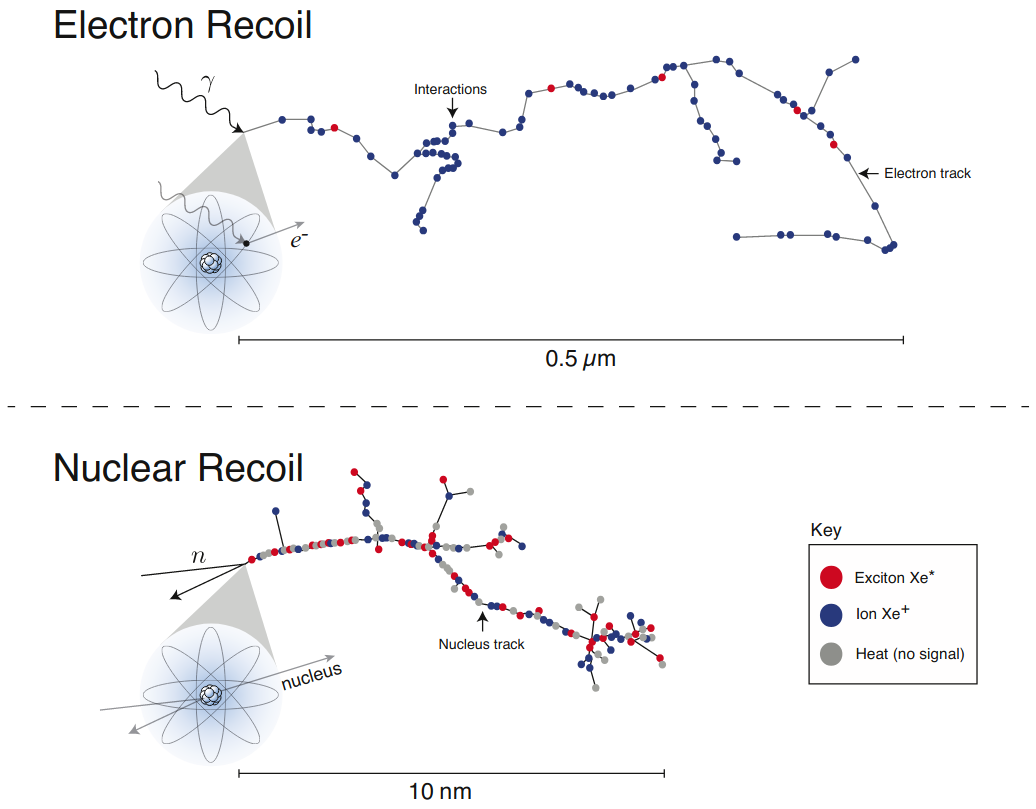
\includegraphics[width=\textwidth]{Figures/LZ/er_nr_tracks.png}
    \caption[Depiction of a 20keV recoil on liquid xenon]{Depiction of 20 keV recoil of electronic recoil (top) and nuclear recoil (bottom) in liquid xenon.
    Figure is from RIVAL simulations by C. Dahl \cite{carldahl_thesis_ref}, with adaptations by C. Fahan \cite{carlosfahan_thesis_ref}.}
    \label{fig:er_nr_tracks}
\end{figure}

\par
The energy deposited in LXe, is split between the atoms and liberated electrons, and so the energy of the recoil, E, can be written as:
\begin{equation}
    E = \frac{W}{L}(N_i + N_{ex})
\end{equation}
Here, W is the W-factor for LXe, generally taken to be 13.7 $\pm$ 0.2 eV \cite{light_and_charge_of_xenon_ref}, though there are more recent measurements indicating it could be as low as 11.5 eV \cite{electron_excitation_energy_of_xenon_ref}. 
N$_i$ and N$_{ex}$ are the number of ionised atoms and number of excited atoms respectively.
L corresponds to the "Lindhard factor" or "quenching" which accounts for the reduced light and charge that's lost to heat.
It is generally taken that L=1 for electron recoils as the heat loss does not vary with energy, allowing the impact this has to be taken into W.
\par
The ratio between the excitation atoms to ionisated atoms allows for the difference between ER and NR events to distinguished, with the resultant number of photons observed differing between the two.
Experimentally, N$_{ex}$/N$_i$ has been measured as $\approx$ 1 for nuclear recoils, and 0.06 for electron recoils \cite{ionisation_to_excitation_ratio_xenon_ref}.

\subsection{Dual-phase Time Projection Chamber}
\par
One such detector design that can utilise the charge-to-light ratio between ER and NR signals are dual-phase time projection chambers (TPCs).
Modern variants of these detectors contain a single element in a majority liquid state with a region of gas above.
\par
An interaction event in a TPC is characterised by two signals.
Firstly a prompt scintillation signal in the liquid region - referred to as the S1.
This is caused by excimers and recombination previously discussed.
Secondly there is a delayed scintillation signal, or S2.
This is observed in the gas phase via electroluminescence.
Both of these signals produce VUV light ($\approx$175 nm) which can be detected by photomultipler tubes (PMTs) or silicon photomulitpliers (SiPMs).
\par
In a typical TPC design, as shown in \autoref{fig:TPC_theory}, an electric field is applied.
This causes electrons that are freed as a result of the interaction to drift upwards towards the gas phase where there is a probability of being extracted into the gas phase and produce and S2 signal.
\par
With PMTs or SiPMs placed at both the top and bottom of the TPC, the size of the interaction signals can be measured.
The preferred unit of this is "photons detected" (phd)\footnote{Historically the signal was measured in photoelectrons (phe) which can be traced back the to first TPC designs of the 1970s \cite{tpc_origins_ref}. However, as there is a non-negligible probability of two photoelectrons being emitted from a single VUV photon in a PMT \cite{pmts_in_xenon_ref}, phd has become more favourable as this can be taken into account.}.

\begin{figure}
    \centering
    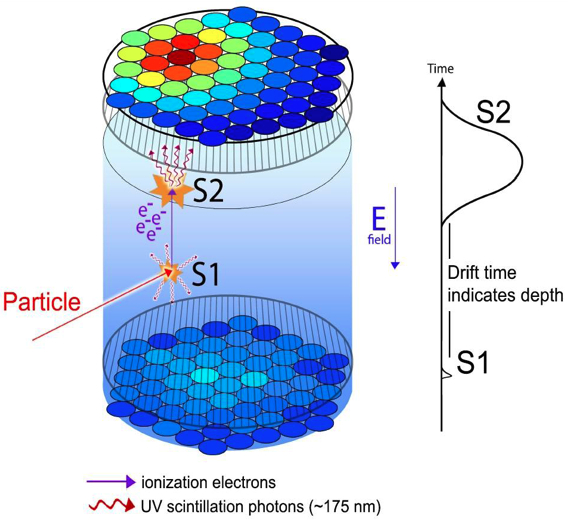
\includegraphics[width=0.6\textwidth]{Figures/LZ/tpc_theory.png}
    \caption{An illustration of the LUX dual-phase TPC \cite{lux_ref}.}
    \label{fig:TPC_theory}
\end{figure}

\par
The position of an interaction in the TPC can be reconstructed using only the S1 and S2 signals.
Firstly the $x-y$ position of an interaction can be reconstructed by the hit-pattern of photons on the gas phase PMTs. 
As the electrons will not deviate significantly from the interaction site, the hit-pattern is a good approximation this location, with ~5mm resolution demonstrated \cite{lux_position_reconstruction_ref}.
The $z$-position can be directly measured by the time difference between the two signals.
This is possible as the electrons reach a terminal velocity rapidly within the LXe, allowing for a resolution ~100$\mu$s \cite{LZ_TechnicalDesignReview_ref}.
This high-resolution position reconstruction allows for the self-shielding of Xenon to be utilised, with the regions of LXe away from the TPC edge experiences a significantly lower background rate.

\par
The size of the two pulses in terms of photons detected, which will now be referred to as S1 and S2, can be related to the underlying quanta which produced them via;
\begin{align}
    n_\gamma = N_{ex} + N_i r && n_e = N_i (1-r) \\
    S1 = n_\gamma G_1(x,y,z) && S2 = n_e G_2(x,y,z)
\end{align}
where both $G_1(x,y,z)$ and $G_2(x,y,z)$ account for the variable light collection efficiency.
It is useful to note that $G_1$ varies between 0 and 1 as the photons will not produce more photons and so the maximum S1 can be is the number of photons produced.
On the other hand, $G_2$ can be greater than 1, as an extracted electron will produce more photons in the GXe.
In fact, $G_2$ is actually dependent upon the length of time an electron spends in the LXe, $t$, the efficiency it has to be extracted on the liquid surface , $\epsilon$, the scintillation yield in the gas phase, $Y_e$, and the LCE in the gas $G_1^{gas}$.
With the full expansion of $G_2$ as;
\begin{equation}
    G_2 = e^{-t/\tau} \epsilon Y_e G_1^{gas}(x,y)
\end{equation}
In typical analysis, the S1 and S2 signals are manipulated to account for the change in LCE with position.
For this, two new quantities are introduced, as the corrected values: S1$_c$ and S2$_c$.
Both the S1 and S2 are adjusted to the centre of the TPC in (x,y).
S1 is also adjusted to a z-position, typically taken to be the centre of the LXe.
\begin{align}
    S1_c = S1 \frac{G_1(0,0,z_c)}{G_1(x,y,z)} && S2_c = S2 \frac{G_1^{gas}(0,0)}{G_1^{gas}(x,y)} e^{t/\tau}
    \label{eq:s1c_and_s2c_full}
\end{align}
S1$_c$ and S2$_c$ are then just both linear relationships to the original quanta, related by a gain factor, $g$, which can be written as:
\begin{align}
    S1_c = g_1 n_\gamma && S2_c = g_2 n_e
\end{align}
With this linear relationship, the reconstructed recoil energy from the event of two pulses (and S1 and S2) becomes:
\begin{equation}
    E_R = \frac{W}{L}(\frac{S1_c}{g_1} + \frac{S2_c}{g_2})
\end{equation}
For NR events, L has an energy dependence.
\par
An example of the possible discrimination between ER and NR from a Xenon TPC is shown in \autoref{fig:er_nr_discrimination} for an arbitrary TPC detector.
The discrimination between ER and NR events is not perfect, with a non-negligible leakage between bands.
The viability of using TPCs for direct dark matter searches can be summarised by two requirements: understanding backgrounds and understanding ER and NR bands.

\input{Chapters/LUXZEPLIN/Figures/er_nr_discrimination}

\par
Modelling of detector responses from S1 and S2 signals have undergone a huge amount of development in recent years, with the Noble Element Simulation Technique (NEST) library leading this.
Both Argon and Xenon detectors are modelled for energy deposits of sub-keV to several MeV \cite{nest_1_ref}.
Additional details of response modelling can be found in \cite{gregrischbieter_thesis_ref, flamenest_ref}.


\iffalse
\par


There are numerous different detector designs to choose from, and the reader is directed towards \cite{direct_detector_designs_ref} for an indepth comparison.


Fortunately, the majority of these will interact in the electron cloud surrounding the nucleus and result in an electronic recoil (ER).
This differs from the nuclear recoil (NR) which would be observed from a WIMP-nucleon interaction.
Therefore to detect a WIMP we are searching for an excess in NR events compared to out background.

\par
Therefore in order to achieve this, a target with minimal isotopes that will decay and cause an excess to be hidden need to be avoided.
Additionally, any detector design should allow for particle discrimination - or more explicit ER and NR discrimination. 
\fi

\section{The LZ Detector}
\par
The LUX-ZEPLIN (LZ) experiment is a second-generation direct detection dark matter experiment, named from it's predecessor LUX, and the ZEPLIN series of experiments which pioneered xenon phase detectors.

The LZ experiment has been primarily designed for the detection WIMP dark matter candidates described in XXX. 
This is primarily done through a dual-phase Time-Project Chamber (TPC).

\par
The LZ experiment is a multi-detector system, which work together to increase the sensitivity to dark matter candidates.
A cut through of the LZ experiment is shown in Figure 

\begin{figure}
    \centering
    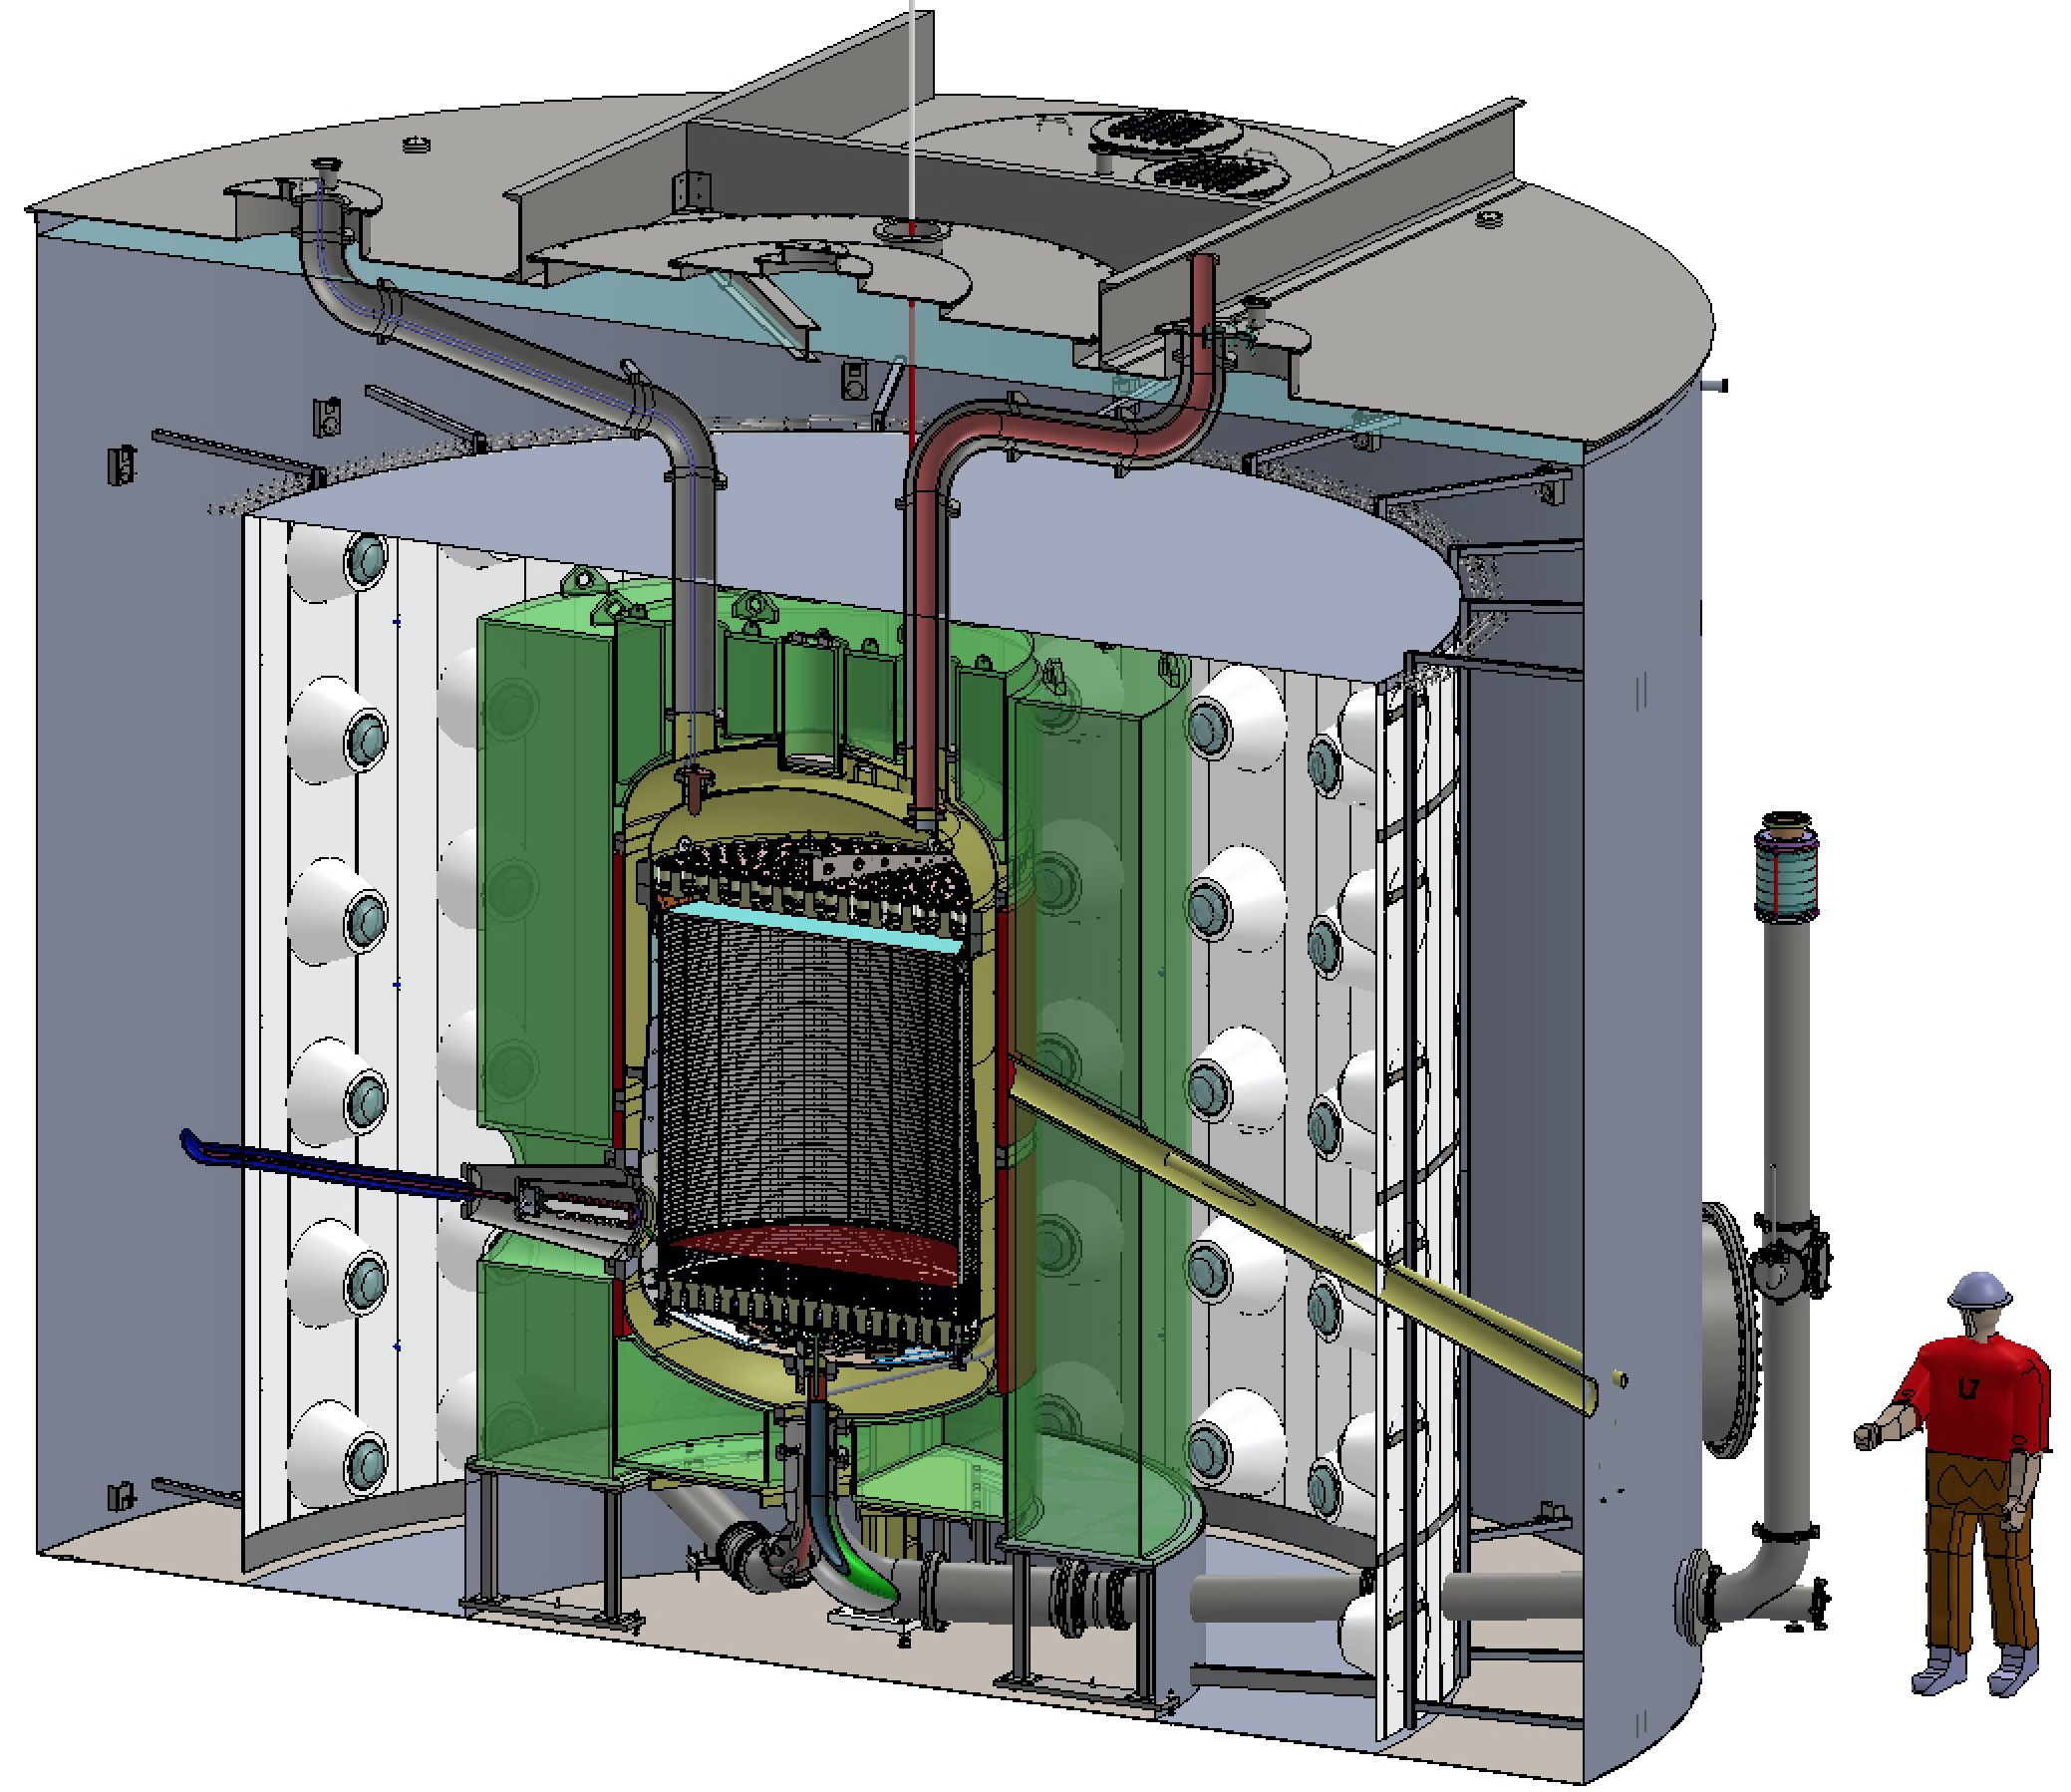
\includegraphics[width=\linewidth/2]{Figures/LZ/LZ_Cut_CAD.jpg}
    \caption{Cross-Section of the LZ experiment. TODO... add numbers. Figure from Ref \cite{LZ_TechnicalDesignReview_ref}}
    \label{fig:LZ_Cut_CAD}
\end{figure}



\par
In the remainder of this chapter, the design and construction of the LZ experiment are detailed with particular emphasis on the TPC, Skin and OD which are relevant for the remainder of this thesis. 
It should be noted that the design is detailed in significant more detail in the Technical Design Review \cite{LZ_TechnicalDesignReview_ref}.

\subsection{TPC}
\par
At the centre of the LZ experiment is the TPC.
It's purpose is the production of S1 and S2 light from particle interactions as previously described in Section XXX.
\par
The TPC is comprised of 2 arrays of photo-multiplier tubes (PMTs); one at the top and one at the bottom, which serve to collect the light from any particle interaction which happens within the TPC volume.
The wall of the TPC is made from PTFE.
\par
The TPC is filled almost entirely with liquid Xenon, with the exception being the gas Xenon pocket just under the top PMT array.

\subsection{Skin}
\par


\subsection{OD}
\par
Surrounding OCV is the outer-detector (OD).
It consists of 10-segments of acrylic tanks (something about UV), which fit around the OCV as shown in Figure XXX.
Together these provide near 4$\pi$ coverage about the OCV.

\par
The OD tanks are filled with a linear akylbenze (LAB) doped with 0.1\% natural Gadolinium (by mass) - which together are refereed to as the Gadolinium Liquid Scintillator (GdLS).



\par



\subsubsection{Design Changes}
\par
During the installation phase of the Acrylic tanks about the OCV, the curvature of the top Acrylic tanks were significantly different to that of the OCV, as such, the top 2 acrylic tanks could not be placed around the 

\par


\subsection{Water}

\subsection{Underground}

\subsection{Backgrounds}

\subsection{Calibrations}
\par
In order for the above experiment to work and have understandable results, a set of calibrations are required to characterise the; energy scale, energy threshold and detection efficiency.
In this section the calibration systems are explained, along with the different sources that are deployable.
A summary of the sources used prior to SR1 are shown in Table XXX. 
Additional sources planed are outlined in the LZ Technical Design Review \cite{LZ_TechnicalDesignReview_ref}

\begin{table}[!htbp]
    \centering
    \begin{tabular}{c|c|c|c}
    \hline
    Isotope       & Interacting particle         & Purpose                    & Deployment \\
    \hline
    ${}^{83m}Kr $ & beta/gamma, 32.1 keV/9.4 keV & TPC (x,y,z)                & Internal  \\
    ${}^{131m}Xe$ & 164 keV gamma                & TPC (x,y,z), Xe skin       & Internal  \\ 
    ${}^{220}Rn $ & various alphas               & xenon skin                 & Internal  \\
    $AmLi       $ & (alpha, n)                   & NR band                    & CSD       \\
    ${}^{252}Cf $ & spontaneous fission          & NR efficiency              & CSD       \\
    ${}^{57}Co  $ & 122 keV gamma                & Xe skin threshold          & CSD       \\
    ${}^{228}Th $ & 2.615 MeV gamma              & OD energy scale            & CSD       \\
    ${}^{22}Na  $ & back-to-back 511 keV gamma’s & TPC and OD sync            & CSD       \\
    ${}^{88}Y Be$ & 152 keV neutron low-energy   & NR response                & External  \\
    $DD         $ & 2,450 keV neutron            & NR light and charge yields & External  \\
    $DD         $ & 272 keV neutron              & NR light and charge yields & External
    \end{tabular}
    \caption{LZ calibration sources that were used for calibration prior to the first science run along with the calibration purpose and deployment method. Table adapted from \cite{LZ_TechnicalDesignReview_ref}.}
    \label{tab:LZ_Used_Calibration_Sources}
\end{table}


\subsubsection{Internal}
\par

\subsubsection{Calibration Source Tubes}
\par

\subsubsection{External}
\par
External sources are sources which are outside of the OCV.

\section{Detector Status}
\par
At the time of writing this thesis, the LZ experiment construction has been completed and the first Science Run completed???
However, it should be noted that due to various construction delays, the calibration and comissioning campaigns were reduced in scope which has implications for the 



\section{LZ Dark Matter Search Strategy}
\par
LZ will search for NR events.
The core cuts are listed below;
\begin{itemize}
    \item \textbf{SS}: DM will only scatter once
    \item \textbf{FID}: to remove wall events
    \item \textbf{ROI}: between 1.65-6.5 keV ER events and 6-30keV NR events, for EFT searches this requirement will inevitably change.
    \item \textbf{Veto}: remove neutrons and $\gamma$'s 
\end{itemize}

\par
LZ will initial run a two dimensional Profile Likelihood Ratio (PLR) fit to distinguish between NR and ER events.
A full description of the PLR used for the WIMP sensitivity projections and SR1 can be found in \cite{LZ_Ibles_LZStats_Thesis_ref}. 
A detailed application to monte-carlo data is described in \cite{jonathannikoleyczik_thesis_ref}.




\subsection{Triggers}
\par
LZ utilises a number of different triggers to determine when data should be recorded, utilising the logic based upon \cite{lux_trigger_logic_ref}, with application to LZ detailed in \cite{nicolasangelides_thesis_ref}.
The three of the triggers are briefly discussed below.


\paragraph{S2 Trigger}
\par
Triggering off the S2 signal in the TPC. 
This is the dark matter search trigger.

\paragraph{OD Trigger}
\par
Triggered by large events in the Outer Detector, focusing on 2.2MeV events from neutron captures on Hydrogen.

\paragraph{Random Trigger}
Also often referred to as the heartbeat trigger, data is recorded for a fixed time.
It can act as a measurement of backgrounds as it is a fixed amount of data recorded periodically.


\par
There are two important features to note;
Firstly the logic is hierarchical, meaning that the Random Trigger will only record when none of the other triggers have switched.
Secondly, the DAQ captures an event when it receives a trigger signal unless there is already an event being captured, or the trigger signal arrives during the hold off time of the previous event.
In practical terms, it means that the Random Trigger can be biased to low energy events if another trigger is active.
For example, in the Outer Detector, if the OD Trigger is active then the Random Trigger will be biased to low energy events as the higher energy events are likely to be encompassed by the OD Trigger.



%\chapter{LUX-ZEPLIN Simulations}
\label{chap:lz_simulations}
\par
In this chapter, important contributions to the development of the LZ simulation capabilities are described.
All of the contributions are specifically for BACCARAT (described in the previous chapter).
These include updates to a light map for S2 photons, as well as early development work to migrate a subset of simulations onto graphics card processors.
Finally updates to a background particle generator are discussed which is used in subsequent chapters.
Sections of this work were supported by Oracle Cloud Computing and have been presented by the author in \cite{se_poster_2018,se_poster_2019_summerschool,se_poster_2019_bristol,SEriksen_IoP_2021_talk_ref}.

\section{S2 Light Map}
\label{sec:s2lightmap}
\par
A single free electron simulated in the LXe with accelerate upwards towards the gas layer due to the electric field.
Once in the gas, the mean photon yield per electron is 825 \cite{NoPhotonsPerElectron}.
As a single scatter event can produce in excess of dozens of electrons, the number of photons which need to be simulated quickly becomes unmanageable, creating a simulation bottleneck.
\par
To get around this, a probabilistic map is used to determine the photon hit pattern on the PMTs and flight time.
For the S2 signal, this is broken up into two sets of probability density functions (PDF).
The first is the likelihood of a photon hitting a given PMT from a given position.
This is essentially the number of photons which hit this PMT divided by the number of photons which hit any PMT.
The second is the likely path taken by the photon, as this effects the time it takes for the photon to hit the PMT, and thus the resultant waveform.
\par
In order to create this light map, large scale simulations of the photons have to be performed at least once.
For every simulation after the map has been generated, there is a significant speed increase as the photons themselves no longer need to be simulated.
In the subsequent simulations, the electron paths are stopped once they reach the liquid surface.
The position of the electron is used to determine the path it would have taken and points along this path are taken to be the photon origin. % to the anode.
The maps are then used along with random numbers and binary searches to determine which PMT the photon hit (if any) as well as how long it took.

\par
A notable downside of this approach is that for different scenarios one may wish to investigate (such as using a different purity of Xenon or the temperature and therefore pressure) then a new light map is needed to account for these effects.
A version of this approach had been used within BACCARAT for a number of years \cite{lz_simulations_ref}, but was outdated due to detector design changes.
The S2 Light Map now in use within BACCARAT, created by the author, took into account the latest geometry and detector physics.

\subsection{S2 Radial Variation} \label{sec:s2radialvariation}
\par
The electric field originates from three electrodes: a cathode grid just above the bottom PMTs, a gate grid just below the surface of the liquid Xenon, and an anode grid in the gaseous Xenon.
In previous simulations it was assumed that the anode and gate were both rigid structures and so had a fixed distance, and electric field between them.
In this case, the number of photons produced in the gas gap by an electron is given by \autoref{eq:s2lightmap_nophotons} and is equal no matter the distance from the centre:
\begin{equation}
    N_{photons/e} = eep \times (\alpha \times E_{gas} \times 1000 - \beta \times P - \gamma) \times d_{gas}
    \label{eq:s2lightmap_nophotons}
\end{equation}
Where $\alpha$, $\beta$ and $\gamma$ are constants, $E_{gas}$ is the electric field in the gas, P is the pressure of the liquid, and $d_{gas}$ is the distance from the top of the liquid to the anode \cite{NoPhotonsPerElectron}.
$eep$ is the electron emission probability at the surface.
%is taken from PiXeY data and fitted to give $eta = -0.03754 \times (eliq^{2}) + 0.5266 \times eliq - 0.84645$, where $eliq$ is the electric field in the liquid Xenon \cite{ElectronExtractionEfficiency}.
The emission probability is included as we want to use the average number of photons per electron.
This simplification was known to be incorrect as a stronger signal\footnote{more photons being detected} should be observed in the detector centre.
Tests conducted at SLAC indicated that there is bending of the wires according to \autoref{WireDeflection} due to the electric field.
\begin{equation}
    x(r,E) = A \sqrt{ \bigg( 1 + \cos{ \Big( \frac{r \pi}{R} } \Big) \bigg) \bigg( B^2 + r^2 \bigg) } \bigg( e^{(r-C)} + 1 \bigg)^{-1} 
    \label{WireDeflection}
\end{equation}
Where R is the radius of the wire, r is the point on the wire and A, B and C are all of the form: $A(E) = \sum_{j=0}^{M} a_{j} E^{j}$. E is the electric field and $a_{j}$ are constants.
As such, the electric field is not constant with radius and thus the number of photons produced by electroluminescence is changed.
\par
These changes were implemented into the simulation package as a scaling on the number of photons which the S2 Light Map is probed for.
Implementing it in this way allows for the resultant signal size to scale with the electric field without having to require a dynamically changing detector grid geometry - which is a much more complex approach.


\section{Graphics Card Simulations}

\par
The probabilistic approach described in the previous section created a significant performance increase. 
However, there are several significant factors which limit the feasibility of using similar methods for the rest of the detector, including;
\begin{itemize}
    \item Optical propagation is required to be performed at least once
    \item Other regions of the detector contain significantly more complex geometry
\end{itemize}
For example, if a probabilistic map were to be applied to the entire TPC Liquid Xenon region, several weeks worth of a full cluster would be required in order to produce the equivalent statistics.
Although there are ways in which this could be reduced - such as Z-line symmetry - the initial overhead remains impractically high.

\subsection{Geant4 Simulations}
\par
Before attempting to improve the speed of simulation, it is important to understand why simulation speed is limited. 
LZ particle propagation simulations are performed in BACCARAT, a software package built upon GEANT4.
In GEANT4, a detector is defined by solid-based modelling or CSG (Constructed Solid Geometry) \cite{geant4_geometry_ref}.
A detector (or scene) is defined by a set of primitive volumes that can be described by some parameters.
An example of this is a sphere; a primitive solid that can be described by a single parameter; radius.
Primitives can be rotated, displaced and combined with other primitives via boolean operations to create more complex solids such as that shown in Figure \ref{fig:csg_geometry_example}.
\begin{figure}[!htbp]
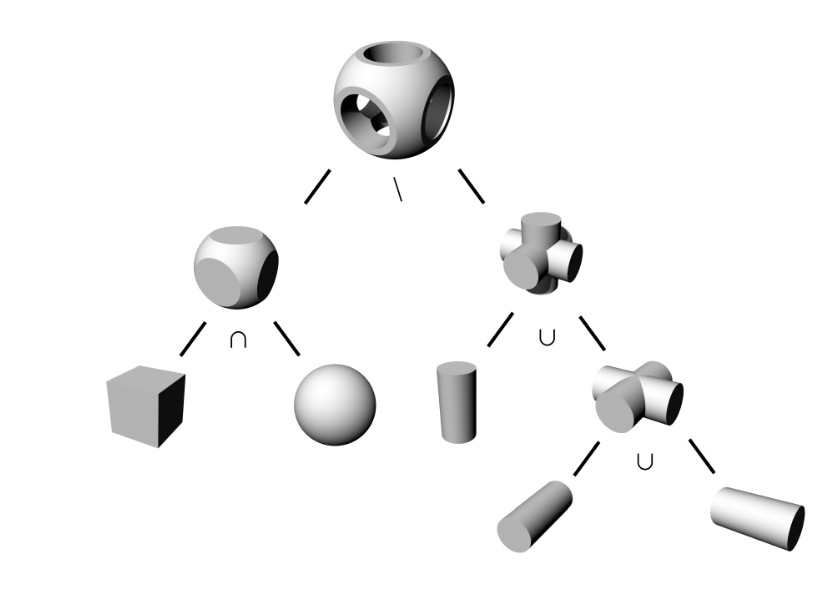
\includegraphics[height=8cm]{Figures/Simulations/csg_geometry.png}
\centering
\caption{Complex solid created from 5 primitive solids using boolean operations; union $\cup$, intersection $\cap$ and difference \textbackslash. Adapted from \cite{csg_geomtry_ref}}
\label{fig:csg_geometry_example}
\end{figure}

\par
In application, the primitive is defined by more than the basic shape parameters (such as radius).
The parameters are used in combination with functions so properties of the solid can be attained.
For example, the solid must be implemented in such as way that it is possible to determine if a point $\vec{x}$ is within the solid, and whether a ray travelling in direction $\hat{d}$ will intersect with the surface of the solid.
These functions have to account for all relevant calculations that relate to a solid.
\par
All of the solids in a scene are contained within a geometry tree.
The top of the tree contains the 'world' volume, inside which there are daughter volumes (which do not overlap with each other).
These volumes can contain there own daughters, and so on.
To the user, this structure is often less obvious with solids connected to each other by logical volumes (LV) and physical volumes (PV).
LVs contain information associated with a solid such as material. 
PVs can contain one or more LV which are given positions are rotations inside of it. 
A PV can be part of a higher up LV.
\par
When a particle is simulated, its track starts inside a volume of a solid which is in the geometry tree.
In the direction of travel, a check must be performed to determine intersections with the volume as well as all immediate daughter volumes.
As each daughter is a subtraction in volume of it's parent, the number of interactions is generally limited.
Even so the number of sibling volumes is often a reliable indicator of particle tracking performance.
Therefore it is logical to for the tree to be as narrow as possible to reduce the number of sibling volumes.
This can be at odds with how a detector is designed, such as if a solid has to have holes for other solids to pass through.
The problem with this is that interior of the solid isn't fully defined by the volume anymore\footnote{An example of this in LZ geometry are the calibration tubes, passing through the water tank, outer detector, and OCV}.
In this case, the geometry tree is widened so that volumes inside become siblings of the problem volume, which in turn increases the number of intersection calculations.
This must be the case to enforce the requirement that each volume is contained entirely by it's mother volume and that it does not overlap with siblings.
\par
GEANT4 in part mitigates this by separating the geometry tree nodes into perpendicular facing boxes, called voxels \cite{geant4_voxel_ref} which are not part of the detector volumes.
During particle propagation, the voxels are checked first for intersections.
If there is an intersection, the detector volumes contained within that voxel are then checked.
Though useful, the voxels are limited to a single level, is performed iterative (1 axis at a time) to save memory and so can hit computation speed.
The GEANT4 approach can be summarised as;
\begin{quote}
    A detector is a tree of nested solids, each composed of some material and mathematically implemented by a particular C++ class.
\end{quote}

\subsection{Optical Simulations}
\par
In addition to particle tracking, the GEANT4 must also handle particle interactions inside a volume which can result in daughter particles that also need to be tracked.
However, in LZ the bottleneck is in the photon propagation, taking up in excess of 95\% of computing time (after using the S2 Light Map).
Optical photon simulations are relatively simple in that no daughter particles that need to be tracked.
There is some probability of a photon being absorbed and re-emitted during propagation, but otherwise photon propagation can be simplified to travelling in a straight line until they reach a boundary.
The simulation is therefore dominated by intersection calculations, or \textit{"has the photon reached the edge of this volume yet?"}.
Therefore increasing the number of these intersection calculations per second will decrease the overall simulation time.
\par
GEANT4-based simulations are performed on CPUs which have typically been designed to minimise task latency; ie the time required to complete any given task.
Although it is possible to multi-thread simulations, it is rarely done due to simulation frameworks often originating decades ago.
An alternative processor widely available is a GPU, which is designed to maximum throughput.
This is achieved by having individual poorer thread performance but by having more threads available\footnote{Additionally, each task should be as independent as possible and require very few resources}.
If a simulation can be moved onto a GPU it will allow for more concurrent tasks that will massively outweigh the slower performance of each task, resulting in more simulations per second
\par
There have been many different attempts to transfer parts or entire simulations on to GPUs, such as Chroma \cite{chroma_whitepaper_ref}, ANTS2 \cite{ants2_whitepaper_ref}, Exascale Computing Project \cite{ExaSMR_whitepaper_ref} and MPEXS \cite{mpexs_whitepaper_ref}.
The majority of these make use of NVIDIA CUDA \cite{cuda_ref}, an application programming interface (API) allowing for GPU hardware to be used for general purpose computing.
\par
Chroma is of particular interest as it was proposed and designed for optical simulations, as it has been utilised in several experiments \cite{chroma_with_tpcs1_ref,chroma_with_tpcs2_ref,chroma_with_tpcs3_ref}, and has more recently received attention by gen-3 direct detection dark matter \cite{DARWIN_GPU_simulations_2022_ref}.
Chroma uses surface-based modelling where a triangle mesh describes the geometry.
This tessellation reduces the number of primitives to one, a triangle which is defined within a the users program in CUDA.
As the surface of a solid is described by a finite set of triangles, this naturally leads to curves not being represented as accurately as the GEANT4 method.
To some extent this can be mitigated by increasing the density of the of primitives, but this is a trade off between accuracy and performance.
The complete geometry is typically defined as a union of non-intersecting closed meshes.
\par
As the geometry structure is broken during tessellation there is no geometry tree which can be navigated.
As a result, Chroma implements a bounding volume hierarchy (BVH) tree structure, a method well used in industry \cite{real_time_collision_detection_ref}.
Crucially, as it is well tested there efficient ways of navigating it.
In a BVH, the lead nodes contain subsets of primitive lists.
To determine if there is an intersection in a BVH, starting at the root node a test is done for an intersection with the box associated with that node.
If an intersection is found, the children are tested for an intersection - analogous to the GEANT4 voxel approach.
The number of intersection calculations is dependant upon the depth of the tree and the number of children per node.
An example BVH is shown in Figure \ref{fig:bvh_example}.
\par
When a simulation wants to be performed, the photon is first generated on the CPU and then copied over to the GPU for propagation.
When the photon is stopped generally by being absorbed at a surface, it is transferred back to the CPU.
Chroma has been shown to be 50-200x speed improvement when compared to GEANT4 single-core processing \cite{chroma_whitepaper_ref,chroma_presentation_ref}.
\begin{figure}[!htbp]
    \centering
    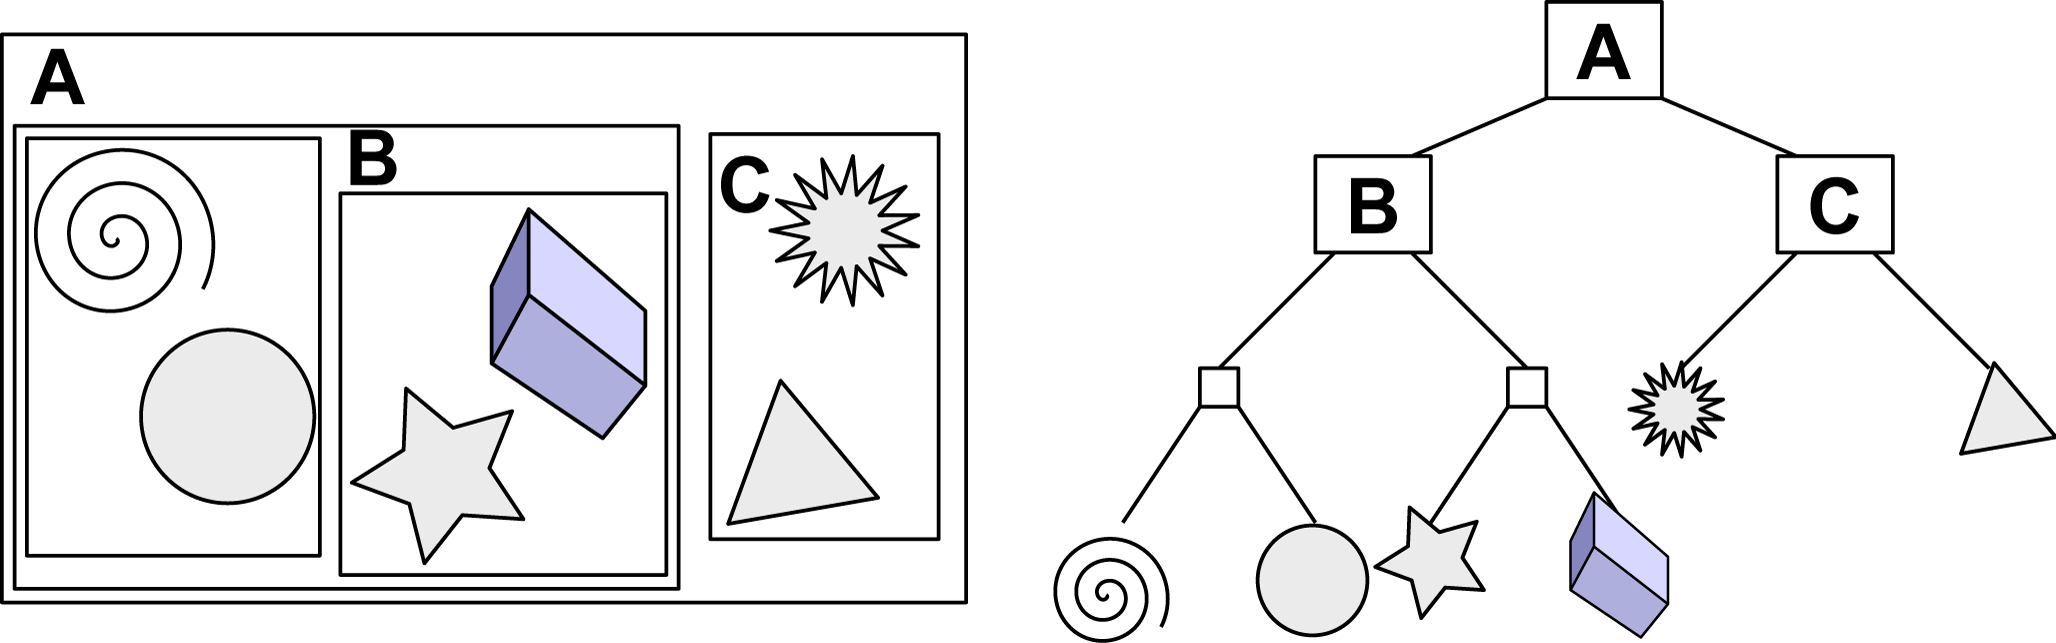
\includegraphics[width=\textwidth]{Figures/Simulations/bounding_volume_hierarchy.png}
    \caption{Example of 2D bounding volume hierarchy. 
             \textbf{Left:} the spacial relationship between solids and bounding volumes.
             \textbf{Right:} the intermediate nodes and the solids in the tree.
             From \cite{bounding_box_ref}}
    \label{fig:bvh_example}
\end{figure}
\par
Despite this, Chroma has some significant drawbacks.
Firstly, the code-base is in python, which makes integration within GEANT4 simulation frameworks impractical which are C++.
Secondly, the inefficient handling of photon generation.
Copying information between the GPU and CPU should be minimised in order to increase performance.
Finally, although tessellation is adequate for some surfaces, many detectors are comprised of exclusively curved surfaces.
In order to achieve adequate accuracy, the number of primitives required begins to eliminate any gain in the processing.
Inspired by Chroma, a separate project was created called Opticks which aimed to tackle the limitations \cite{Opticks_Paper_2017_ref,Opticks_CHEP_2019_ref,Opticks_CHEP_2021_ref} which is what was chosen here.

\subsection{Opticks}
\par
Where as Chroma is built around CUDA, Opticks\footnote{Yes it is a confusing name} is built around NVIDIA OptiX \cite{nvidia_optix_paper_ref}, a ray tracing API.
As most ray-tracing algorithms require only a small set of operations, OptiX allows the user to build applications from a small set of CUDA programs.
These programs can define the ray generation, intersections with surfaces, camera characteristics and so on.
This means that a primitive can be defined mathematically correct.
Additionally, more complex solids can be created by CSG as in GEANT4.
The primitives are described as boundaries  \cite{real_time_collision_detection_ref}.
\par
OptiX uses an acceleration structure which sorts primitives into spatial groups.
This is then used by a traversal algorithm to search for primitives that potentially intersect with a ray\footnote{OptiX provides acceleration to the geometrical intersection, not the intersection itself.}.
All details of the creation and traversing of the acceleration structures are handled internally by OptiX using user defined bounding box programs.
The creation of these groups remain a key research area in ray tracing \cite{NVIDIA_OptiX_GPU_Ray_Tracing_ACM_paper_ref,accelerated_bvh_ref}.
\par
Opticks is an open-source framework designed to convert GEANT4 geometry into an appropriate GPU form and perform photon simulations.
This includes the detector geometry and optical properties.
To allow for this, Opticks has ported the majority of GEANT4 primitives into CUDA equivalent ones \cite{Opticks_CHEP_2019_ref}.
Opticks converts the geometry tree used by GEANT4 into a boundary based geometry model.
Each CUDA primitive is defined by an intersection calculation which are based of those in \cite{real_time_collision_detection_ref} and a bounding box program.
All possible intersection directions are defined for each primitive; ray inside travelling outward, ray outside travelling inward.
The intersection decision of a solid is based upon \cite{CSG_Intersection_ref}, using a recursive algorithm.
However, OptiX does not allow for recursive intersection programs, so Opticks uses a always-left traversal method creating an iterative approach.
\par
The resultant Opticks geometry tree is a set of binary trees with primitive leaves and operator nodes.
Practically speaking this is as a NumPy serialised arrays, where each solid is defined by it's own binary tree \cite{Opticks_Paper_2017_ref}, and these trees are indexed together based upon the structure.
The nodes contain an rotations.
Opticks navigates the binary tree via bitwise manipulation\footnote{parent $=i >> 1$, left child $= i << 1$, right child $(i<<1)+1$}.
This means that the tree height should be kept relatively low in order to reduce the number of bits required to navigate it.
As such, Opticks has a limit of 7 as $(1 << (7 + 1)) - 1 = 255$ which allows for comparison with 256-bit CPU approaches as well not limiting memory use.
Opticks achieves this on trees which are not already of this height by attempting to balance them.
This is described in more detail in the following section.
\par
During the geometry conversion, Opticks attempts to highlight duplicate solids.
This way, when the geometry is uploaded to the GPU, the tree only needs to be uploaded once, and instancing is used which provides some memory saving \cite{Opticks_CHEP_2019_ref}.
Opticks also allows for geometry caching via NumPy serialisation \cite{Opticks_Paper_2017_ref} to avoid having to perform this conversion which is often computationally intensive, more than once.
\par
In addition to the solids conversion, material and boundary properties are also translated as NPY which are indexed to which solids they refer to.
Separate CUDA programs handle the ray behaviour when influenced by these properties.
\par
A key benefit of Chroma over opticks is that it relies upon CUDA only, and is therefore not a significant challenge to port to OpenCL \cite{chroma_whitepaper_ref}.
This will allow for non-NVIDIA GPU workflows.
However, for the foreseeable future, the performance will still lack significantly behind OptiX.
Additionally, all of the clusters which LZ current use or plan to use contain NVIDIA GPUs, with the primary upcoming computing resource Perlmutter using NVIDIA A100 GPUs \cite{perlmutter_ref}.
\par
In the next sections the translation of the LZ geometry is described along with initial performance metrics.
The proposed integration into the LZ simulation framework is discussed in \cite{SEriksen_Opticks_CHEP_2021_ref}.

\subsection{LZ Geometry Conversion}
\par
In order to use the LZ geometry, it must first be extracted from GEANT4 where it is defined.
The simplest way to export a GEANT4 defined geometry is via a GDML (Geometry Description Markup Language) file \cite{GDML_USER_GUIDE_ref}.
GDML is a subset of XML which is designed to describe the geometry by describing a detector as a series of trees which correspond to the hierarchy of volumes \cite{GDML_USER_GUIDE_ref}.
A small exert of the LZ geometry GDML is shown below;
\begin{lstlisting}[backgroundcolor=\color{lightgrey},
                   language=XML, xleftmargin = 0.5cm]
<volume name="expHall_log0x1051db0">
  <materialref ref="vacuum0xea27f0"/>
  <solidref ref="expHall_box0x1152c20"/>
  <physvol name="subVol0x106c220">
    <volumeref ref="subVol_log0x1058260"/>
    <position name="subVol0x106c220_pos" unit="mm" x="0" y="0"
       z="1189.395000001"/>
  </physvol>
</volume>
\end{lstlisting}
In this extract, we can see the logical volume \textit{expHall\_log0x1051db0} which is filled with the solid box, \textit{expHall\_box0x1152c20}, that is made of a vacuum.
Inside this box a physical volume has been placed, \textit{subVol0x106c220} which contains the logical volume \textit{subVol\_log0x1058260}.
\par
The structure of the GEANT4 geometry is as PV/LZ/PV/LV which means that if put into a geometry tree that isn't in the same style as GEANT4 will require twice as many nodes to properly navigate it than is actually necessary.
As the PV contains the placement of the LV and what the sibling volumes are the PV placement information can be propagated into the LV and removed.

\par
The LZ detector contains a number of solids which are of significant complexity that the tree describing them is greater than 7 in depth.
These are typically unbalanced due to the way in which they were created in GEANT4, for example where a shape contains many holes (and therefore multiple subtractions).
These would likely have been implemented as one subtraction at a time from the primary solid.
A balanced approach would be to union subtractions together and then perform a single subtraction.
Figure \ref{fig:UnionSolidBinaryTree} describes a solid made up of 4 primitive solids an unbalanced and balanced tree.
During the geometry conversion, Opticks recognises large trees and attempts to balance them via De Morgan's law.
This results in a tree with only union, intersection operators and complemented primitives.
These complemented primitives are conceptually "inside-out", but are implemented as just flipping the solid normal and classifying an intersection "Miss" becoming a volume "Exit".
\begin{figure}[!htpb]
\centering 
\begin{tikzpicture}[level distance=1.5cm,
  level 1/.style={sibling distance=3cm},
  level 2/.style={sibling distance=1.5cm}]
  \node {u}
    child {node {u}
      child {node {u}
        child {node {ps}}
        child {node {ps}}}
      child {node {ps}}}
    child {node {ps}};
\end{tikzpicture}
\begin{tikzpicture}[level distance=1.5cm,
  level 1/.style={sibling distance=3cm},
  level 2/.style={sibling distance=1.5cm}]
  \node {u}
    child {node {u}
      child {node {ps}}
      child {node {ps}}
    }
    child {node {u}
    child {node {ps}}
      child {node {ps}}
    };
\end{tikzpicture}
\caption{Binary tree representation of a simple solid comprised of the union (u) of 4 primitive solids (ps). \textbf{Left:} Unbalanced tree. \textbf{Right:} Balanced tree.}
\label{fig:UnionSolidBinaryTree}
\end{figure}
\par
This approach works for most unbalanced trees, however it does work for some of LZs components.
Around the PMTs in the TPC exists a titanium plate and PTFE lining.
The titanium plate holds the PMTs in place, and the PTFE creates a reflective surface for photons on top of the titanium.
As the solids must have space for each PMT they are implemented as one solid with each hole subtracted out.
The tree for this (as defined in GEANT4) is shown in Figure \ref{fig:Opticks_unbalanced_shape}.
\begin{figure}[!htbp]
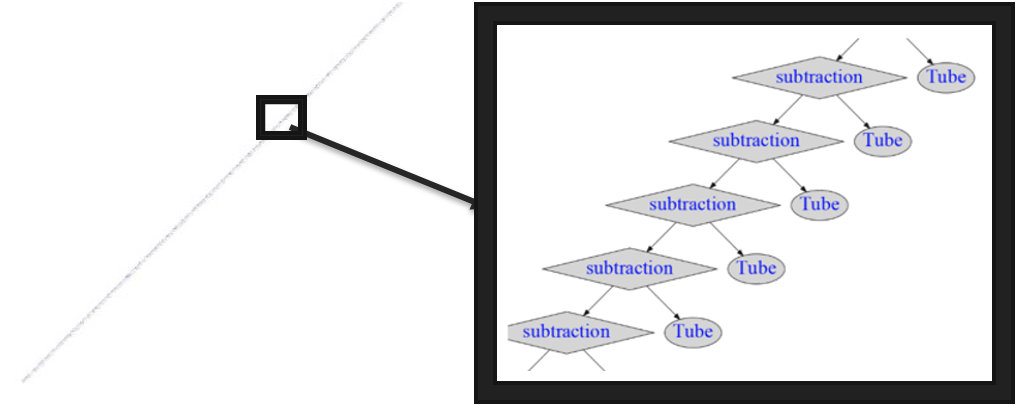
\includegraphics[width=\textwidth]{Figures/Simulations/unbalanced_ptfe.png}
\centering
\caption{Visual Representation of titanium top plate solid, comprised of a single G4Tube and 283 G4Tube subtractions. Kindly created by B. Krikler.}
\label{fig:Opticks_unbalanced_shape}
\end{figure}
For the top titanium plate this implementation would require $(1 << (253 + 1))-1 = 2^{254} - 1$ nodes, an impractically large number.
If perfectly balanced, this would still have a depth of 8.
This raises a problem as it requires the memory required to increases beyond a practical level with 512-bits required to describe the tree.
A method inspired by JUNO was adopted in order to handle this \cite{Opticks_CHEP_2021_ref}.
A primitive was created which defined the solids themselves, so rather than being comprised of a CSG tree of mulitple primitives, the trees became a single node of one primitive.
The basic creation process is shown in Figure \ref{fig:Opticks_PTFE_primative}.
In order the simplify the primitive code, the 3D shapes were reduced to 2D-intersections.
3D is then introduced by duplicating adding a Z-range in which the intersection needs to be evaluated.
Additional details of this approach at at \cite{optix_primitive_code_ref}.
Given the depth of these primitives, they were also likely a hold up in GEANT4 simulations, particularly the S2 light simulations mentioned in Section \ref{s2lightmap}.
In a branch of LZ code using GEANT4.10.6, these 4 solids were converted into G4MultiUnion solids which have built-in optimisation \cite{multiunion_ref}\footnote{At time of writing, LZ code uses GEANT4.10.3.p02 and this feature was introduced in GEANT4.10.4}.
This provided a 56\% decrease in simulation time.
\begin{figure}[!htbp]
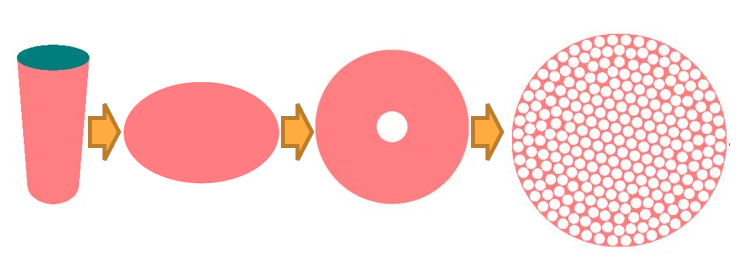
\includegraphics[width=0.7\textwidth]{Figures/Simulations/opticks_PTFE_primative.png}
\centering
\caption{Development stages for representing a 3D disc with multiple holes and a 2D disc with holes as defined within OptiX intersection program.}
\label{fig:Opticks_PTFE_primative}
\end{figure}

\par
The LZ geometry is comprised of in-excess of 900,000 shapes, and although there is some duplication, this only reduces down to around 14,000 shapes.
Given the complications with solids such as the titanium plate, then scope of the conversion was limited to just the TPC and Skin.
This to 9,000 unique shapes which is 30-times greater than that of experiments which have previous used Opticks such as JUNO and DayaBay \cite{Opticks_CHEP_2021_ref}.
The completed TPC conversion is shown in Figure \ref{fig:OpticksLZTPC}.
\begin{figure}[!htbp]
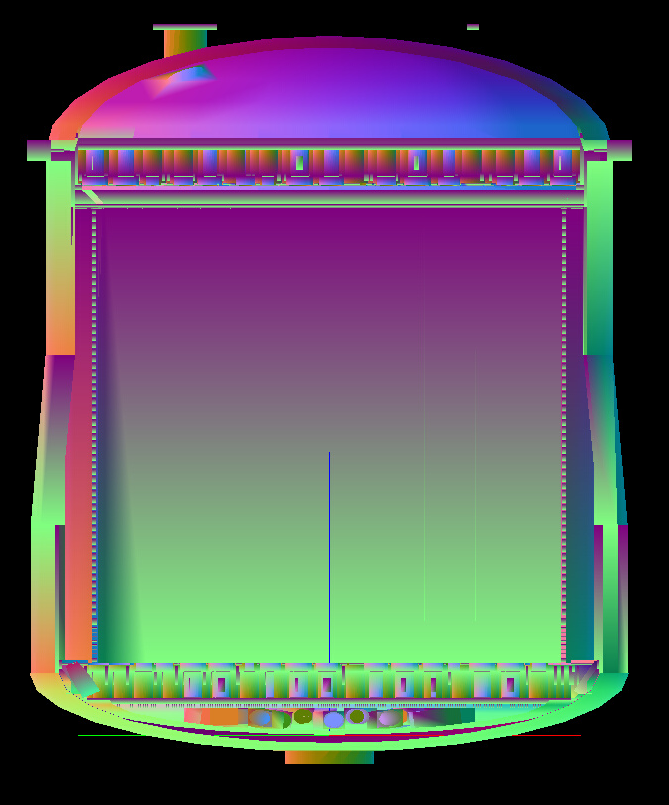
\includegraphics[width=8cm]{Figures/Simulations/LZ_In_Opticks.png}
\centering
\caption{TPC of LZ raytraced. Translated from Geant4 GDML file into NPY set using Opticks and viewed within Opticks via the OpenGL Buffer.
The blue, green and red lines towards the bottom of the figure are the axis.}
\label{fig:OpticksLZTPC}
\end{figure}

\subsection{Performance and Outlook}
\par
As LZ utilised multiple clusters across the globe, the computing environment is kept constant by use of containers.
As such, as part of this work Opticks was containerised \cite{opticks_docker_ref} which also acted in part as a way of removing legacy code and requirements.
NVIDIA OptiX 6.5.0 and CUDA 10.2 were chosen as they were the newest fully supported versions within the Opticks framework.
Making use of NVIDIA container runtime to access the GPU, the container was successfully run - with graphics - on a range of computing resources.
This allowed for integration into the LZ framework to begin, the plan for which is described in \cite{SEriksen_Opticks_CHEP_2021_ref,lz_status_with_opticks_ref}.
\par
As the geometry was cut down during the conversion, the most valuable test that could be performed was a comparison to the S2 Light Map (Section \ref{s2lightmap}).
For this, 200,000 photons per generated as a photon bomb as shown in Figure \ref{fig:OpticksLZTPC_S1_Photons}.
On a Tesla T4 GPU, after a 4-minute initialisation time using the serialised geometry, 200,000 photons per second were generated and propagated.
This marks a 720x improvement over single-core Geant4 propagation where 277 photons per second were generated and propagated for the S2 Light Map or 360x improvement over the expected gain when compared to GEANT4.
On the production clusters - such as Perlmutter - the performance is expected to increase.
This improvement highlights one of the reasons for choosing an OptiX-based approach rather than pure CUDA, as the improvement would have been closer to 200x such as was shown in \cite{chroma_presentation_ref}.
However, it still lacks behind the improvement demonstrated using Opticks in \cite{Opticks_CHEP_2019_ref}, though this is primarily due to higher grade GPUs being used with RTX-cores.
With the newer NVIDIA OptiX 7.0.0+, the algorithms are expected to continue to increase in speed which should provide additional performance.
Unfortunately the accuracy of this simulation has not been ascertained yet but the speed improvement is a promising result.
\begin{figure}[!htbp]
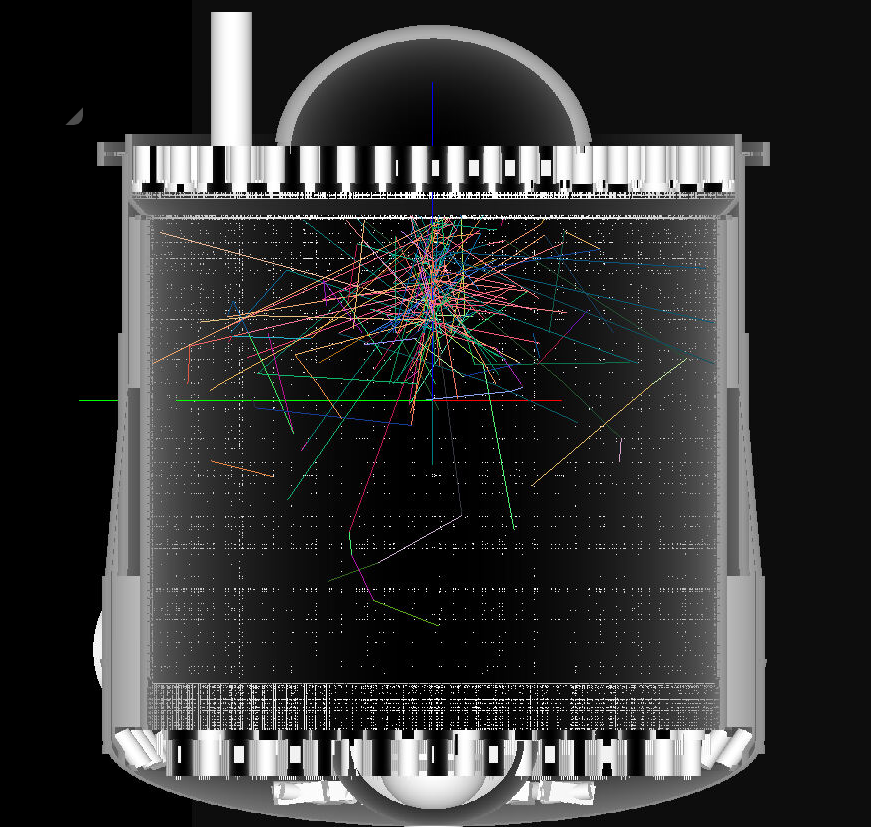
\includegraphics[width=10cm]{Figures/Simulations/LZ_S1_photons_In_Opticks.png}
\centering
\caption{TPC of LZ raytraced. Translated from Geant4 GDML file into NPY set using Opticks and viewed within Opticks via the OpenGL Buffer.
The blue, green and red lines extended outside the OCV are the axis. After each reflection a photons colour has been set to change.}
\label{fig:OpticksLZTPC_S1_Photons}
\end{figure}

\section{Cavern $\gamma$ Generator}
\label{sec:cavern_gamma_generator}

\par
Although the LZ detector has been constructed underground to limit cosmic radiation, it does come with a drawback of being in a mine with a non-negligibly radioactive rock and the shotcreat and gravel within the David Cavern.
LZ is not unique in this, it is a problem highlighted in a number of other underground experiments \cite{cavern_gamma_annual_modulation_CoGeNT_ref, cavern_gammas_in_Soudan_mine_ref}, with an annual modulation mimicking dark matter potentially seen in \cite{cavern_gamma_annual_modulation_CoGeNT_ref}.
The rate of this has been measured and can be attributed to the shotcreat and gravel \cite{LZ_Gamma_Ray_Background_ref}. 
One of the most significant sources of background come not from any internal component but rather from $^{238}U$, $^{232}Th$ and $^{40}K$ decays from the cavern in which the LZ detector exists \cite{LZ_Gamma_Ray_Background_ref}.
However, this is a computationally intensive process to simulation $\gamma$'s where the majority will not reach the actual detector.
To compensate, a generator for these $\gamma$'s was created - and originally described in \cite{rg_generator_ref} but summarised below.
The generator is a created by performing simulations of the decay chains originating in the shotcreat and gravel.
The $\gamma$'s which reach a pre-defined surface are saved.
A second stage simulation is then performed where each of the saved $\gamma$'s is generated a number of times and then saved at another pre-defined surface.
This boost occurs a number of times, until a generator surface.
When subsequent simulations are performed, these saved $\gamma$'s are randomly sampled. 

\par
In order to perform the For the creation of the generator additional cavern properties are added to the simulation.
Namely; a steel pyramid and gravel beneath the water tank, and a layer of shotcreat.
These adaptions are shown in Figure \ref{fig:Cavern_Geometry}.

\begin{figure}[!htbp]
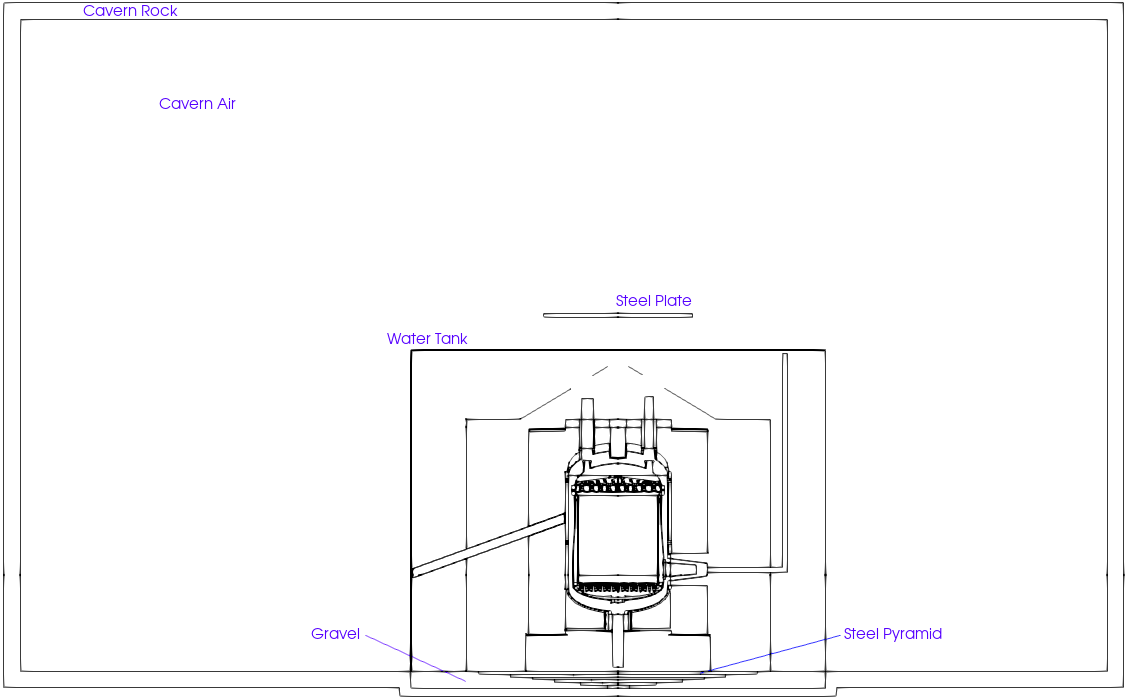
\includegraphics[width=\textwidth]{Figures/Geometry/cavern_geometry_with_markings.png}
\centering
\caption{LZ detector geometry slice with additional cavern geometry. OD PMTs are not seen present as they do not lie in this plane. The red dot marks (0,0,0).}
\label{fig:Cavern_Geometry}
\end{figure}

\par
Although as mentioned in \cite{scotthaselschwardt_thesis_ref}, a generator for the Davis Cavern $\gamma$'s existed, it had a number of flaws.
Firstly, no $\gamma$ below 2MeV was saved.
This meant that $^{40}K$ was not included and so the resultant expected rates being lower than expected.
Additionally, the generator was created using a version of GEANT4 which the rest of the simulation chain had moved on from; GEANT4.9.5 to GEANT4.10.3.p02. 
This motivated the creation of a new generator.

\par
The parameters of the new generator are shown in Table \ref{tab:cavern_gamma_generator_parameters} and a comparison of the energy distribution of the old and new generators is shown in Figure \ref{fig:cavern_gamma_energy_distribution}.
Although it can be seen that the previous generators had a maximum $\gamma$ energy of 10MeV, it also highlights a significant change between GEANT4.9.5 and GEANT4.10.3.p02.
That is, an increased rate above 9MeV.
These $\gamma$'s are predominately from ($\alpha$,$\gamma$) reactions such as $O + \alpha \to Ne + \gamma$.
These are of particular concern as they have the potential to mimic dark matter.
Conversely, they may produce large signals in the OD which would trigger a veto, reducing the detector livetime.
Since this version of GEANT4, there have been new studies of the ($\alpha$,$\gamma$) cross-section in other underground laboratories, such as in \cite{cavern_gammas_in_Soudan_mine_ref}.
Generally, very little attention has been given to ($\alpha$,$\gamma$) rates, and so it is possible that the observed rate may differ significantly from that shown here as although in Figure \ref{fig:cavern_gamma_energy_distribution} the largest difference is at higher energy $\gamma$'s, as was shown in the Sudan Mine \cite{cavern_gammas_in_Soudan_mine_ref}, the rate of sub-6MeV $\gamma$'s may also change significantly. 

\par
The livetime ($l$) for a simulation can be determined then by $l_{\text{simulation}} = \frac{\text{n.} \gamma_{\text{simulated}}}{\text{n.} \gamma_{\text{generator}}} * \text{l}_{\text{generator}}$
In short, this means that every $\gamma$ in the generator represents roughly 130000 decays from the rock, and so is a significant computational saving.


\begin{table}[!htbp]
    \centering
    \begin{tabular}{c|c|c|c}
        Generator    & Activity (Bq/kg) & Boost per surface & Generator livetime (days)  \\ \hline
        ${}^{40}K$   & 216              & 28                & 57.72                      \\
        ${}^{238}U$  & 29.1             & 34                & 60.26                      \\
        ${}^{232}Th$ & 12.5             & 70                & 60.66
    \end{tabular}
    \caption{Parameters used in generator creation. Activity rates are from \cite{LZ_Gamma_Ray_Background_ref}.}
    \label{tab:cavern_gamma_generator_parameters}
\end{table}


\begin{figure}[!htbp]%
\centering
\begin{tikzpicture}
\centering
    \begin{groupplot}[%view={0}{90},
    group style = {group size = 2 by 1,
                   horizontal sep=1.0cm}]
    \nextgroupplot[
            xlabel=Energy (keV),
            ylabel=Rate (Hz/15keV),
            width=0.5\textwidth, height=6cm,
            xmin=0, xmax=14000,
            minor y tick num=8,
            ymode=log, ymin=1e-6, ymax=10,
            grid=major,]
            \addplot[green, mark=none]
                    table [x=Bins,y=Weights]
                    {Data/Simulation_Analysis/Cavern_Gammas/old_gamma_generator_th232.dat};
            \addplot[blue, mark=none]
                    table [x=Bins,y=Weights]
                    {Data/Simulation_Analysis/Cavern_Gammas/old_gamma_generator_u238.dat};

        \nextgroupplot[
            xlabel=Energy (keV),
            width=0.5\textwidth, height=6cm,
            xmin=0, xmax=14000,
            yticklabel pos=right,
            minor y tick num=8,
            ymode=log, ymin=1e-6, ymax=10,
            grid=major,
            legend style = { column sep = 10pt, legend columns = -1, legend to name = Cavern_Gamma_CommonLegend,}]
            \addplot[green, mark=none]
                    table [x=Bins,y=Weights]
                    {Data/Simulation_Analysis/Cavern_Gammas/new_gamma_generator_th232.dat};
            \addplot[blue, mark=none]
                    table [x=Bins,y=Weights]
                    {Data/Simulation_Analysis/Cavern_Gammas/new_gamma_generator_u238.dat};
            \addplot[red, mark=none]
                    table [x=Bins,y=Weights]
                    {Data/Simulation_Analysis/Cavern_Gammas/new_gamma_generator_k40.dat};
            \legend{${}^{232}Th$, ${}^{238}U$, ${}^{40}K$}
            
    \end{groupplot}
    \node at ($(group c2r1) - (group c1r1) + (-0.5cm, 5.0cm)$) {\ref{Cavern_Gamma_CommonLegend}};
\end{tikzpicture}
\caption{Generator $\gamma$ energies. \textbf{Left:} Previous generator. \textbf{Right:} This work.}
\label{fig:cavern_gamma_energy_distribution}
\end{figure}


\par
Additionally it was noticed during the comparison that in the previous generator the distribution was not a cylinder but rather had mistakenly been created as a table.
The result of this is that the $\gamma$ distribution is biased to the top and bottom of the detectors more so than it would otherwise be.
This is highlighted in Figures \ref{fig:cavern_gamma_energy_distribution} and \ref{fig:cavern_gamma_position_distribution}.



\begin{figure}[!htbp]
    \centering
    
\includegraphics[width=0.5\textwidth]{Figures/Placeholder.png}
    \caption{Simulated cavern $\gamma$ energy deposit locations in the OD normalised to rates from \cite{LZ_Gamma_Ray_Background_ref}. \textbf{Left:} Previous generator. \textbf{Right:} newly created generator.}
    \label{fig:cavern_gamma_position_distribution}
\end{figure}


\par


\begin{figure}[!htbp]
    \centering
    
\includegraphics[width=0.5\textwidth]{Figures/Placeholder.png}
    \caption{Change in OD rate between different generator versions}
    \label{fig:cavern_gamma_rate_difference}
\end{figure}



%\chapter{LZ Outer Detector}
\par
In this Chapter the OD is described along with an insight into its subsystems.
The construction and installation underground is discussed.
Simulated veto performance at presented here.

\section{The LZ Outer Detector} \label{OD_info}

\par
LZ uses linear akylbenze (LAB) - the generic term for this class of chemical compositions - as the liquid scintillator.
In this, neutron capture happens on the hydrogen; $n + p \xrightarrow{} d + \gamma$ with a capture constant of 200$\mu$s \cite{LZ_TechnicalDesignReview_ref}.
The hydrogen capture produces a single 2.2MeV $\gamma$.
\par
The scintillator in the OD is doped with 0.1\% (by mass) by Gadolinium.
This provides 

\begin{enumerate}
    \item cross section 49kb: (61kb for $Gd^{155}$ and 254kb for $Gd^{157}$)
    \item capture energy release: 8536.39keV ($Gd^{155} \xrightarrow{} Gd^{156}$) and 7937.39keV ($Gd^{157} \xrightarrow{} Gd^{158}$)
    \item More released particles (4.7, $\gamma$'s and $e^{-}$)
    \item neutron-capture time = 30$\mu$s
    \item 9000 optical photons per MeV. Not sure where this number has some from
\end{enumerate}

\par
LZ dopes with 0.1\% by mass (0.23 - 0.34\% by number)

\par
In addition to the gadolinium doping, the scintillator is also made up of two wavelength shifters; a primary shifter (or fluor) and a second wavelength shifter.
The fluor is 2,5-diphenyloxazole (PPO); an organic scintillator which converts shorter wavelength light to longer wavelength light. 
This has a spectrum peak at 385nm (UV).
The second wavelength shifter is 1,4-bis(2-methylstyryl(benzene)) (Bis-MSB). 
Bis-MSB absorbs the PPO scintillation and emits with peak of around 410-425nm.
The reason for the second shifter is that the wavelength emitted is absorbed less by the LS and is closer to the PMT response.
Importantly, the absorption length of the GdLS increases from 1m to in excess of 10m in that range - and continues to rise.

\par
The complete chemical components in the GdLS is shown in Table \ref{tab:GdLS_Components}.

\begin{table}[!htbp]
    \centering
    \begin{tabular}{c | c | c | c}
    \hline
    {Component (referred as)} & {Purpose} & {Weight (g/mol)} & {Mass (g)} \\ \hline
    $C_{17.14}H_{28.28}$ (LAB) & n,g & 234.4  & 853.55 \\
    $C_{15}H_{11}NO$ (PPO) & primary wavelength shifter & 221.3 & 3.00 \\
    $C_{24}H_{22}$ (Bis-MSB) & wavelength shifter & 310.4 & 0.015 \\
    $C_{9}H_{17}O^{-}_{2}$ (TMHA) & chelation agent & 157.2 & 2.58 \\
    natural gadolinium (Gd) & neutron capture & 157.3 & 0.86 
    \end{tabular}
    \caption{Components in 1L of GdLS}
    \label{tab:GdLS_Components}
\end{table} 

\par
Table \ref{tab:Gadolinium_abundances_and_crosssections} contains the natural abundances of gadolinium.

\begin{table}[!htbp]
    \centering
    \begin{tabular}{c | c | c}
    \hline
    {Isotope} & {Abundance (\%)} & {Cross-section (b)} \\ \hline
    $Gd^{152}$ & 0.2 & 735 \\
    $Gd^{154}$ & 2.18 & 85 \\
    $Gd^{155}$ & 14.80 & 60900 \\
    $Gd^{156}$ & 20.47 & 1.8 \\
    $Gd^{157}$ & 15.65 & 254000 \\
    $Gd^{158}$ & 24.84 & 2.2 \\
    $Gd^{160}$ & 21.86 & 1.4

    \end{tabular}
    \caption{Gadolinium natural abundances and thermal neutron capture cross-sections \cite{Gadolinium_abundances_and_crosssection_ref}}
    \label{tab:Gadolinium_abundances_and_crosssections}
\end{table} 

\paragraph{Other Properties}
It is also worth noting that proton scatters and $\alpha$'s have quenched scintillation signals.
For the proton, it is most easily described by the effect of neutron collisions.

\par
In the lab-frame, the ratio between a neutrons initial energy ($E$) and final energy ($E'$) when colliding with an at rest nucleus of mass A follows;
\begin{equation}
    \frac{E'}{E} = \frac{A^2 + 1 + 2A\cos{\theta}}{(A + 1)^2}
\end{equation}
where $\theta$ is the scattering angle in the CoM.
Now, if the nucleus is a hard sphere, so independent of $\theta$, then an elastic scatter follows
\begin{equation}
    E^{'} = E(\frac{A-1}{1})^{2}
\end{equation}
If A = 1 (so is a proton), then it reduces further to $E^{'} = \frac{1}{2}E$, meaning that the neutron loses half its energy on average.
The scattered proton has energy $E - E^{'}$ and is quenched.



\subsection{Neutrons in GdLS}

\subsubsection{background neutrons}
\par
Maybe this and DD neutrons into a separate section before GdLS section?

\subsubsection{DD neutrons}
\par
10,000 DD simulations have been done - a mono-energetic neutron source which LZ will be using for calibration purposes.
Neutrons are emitted at 2.45MeV.

\par
From these simulations (performed on BACCARAT release 6.2.1).
Table \ref{tab:Where_neutrons_go} shows the number neutrons which enter the scintillator and have their final stage there.
The vast majority of the neutrons emitted enter and are captured in the parts of the detector immediately surrounding where it originated.
Importantly, only 23\% of neutrons which remain in the detector finish in the scintillator.
This could be Gd-capture, H-capture, or something else.

\begin{table}[!htbp]
    \centering
    \begin{tabular}{c | c | c  }
    \hline
    {Final Volume}  & {Where all go (\%)} & {Where all go - ignoring OutOfWorld (\%)} \\ \hline
    WaterAndPMTs & 33.59 & 42.55 \\
    OutOfWorld & 21.06 & - \ \\
    ScintillatorCenter & 18.75 & 23.75 \\
    PVCNeutronTube & 15.06 & 19.08 \\
    LiquidXenonTarget & 2.39 & 3.03 \\
    ScintillatorTank & 2.16 & 2.74 \\
    OuterTitaniumVessel & 1.93 & 2.44 \\
    LiquidSkinXenon & 1.27 & 1.61 \\
    InnerTitaniumVessel & 1.19 & 1.51 \\
    WaterTank & 1.12 & 1.42 \\
    SteelNeutronTubeCaps & 0.8 & 1.01 \\
    Other & 0.68 & 0.86 
    \end{tabular}
    \caption{The volume within the detector where DD neutrons have their final step. OutOfWorld indicates that the neutron left the detector area and so the simulation stopped as it's path is not relevant. Other refers to any other part of the detector.}
    \label{tab:Where_neutrons_go}
\end{table} 

\par
Focusing on the neutrons which finish in the scintillator volume, we can in Table \ref{tab:Where_gdls_neutrons_go} that 78\% of neutrons which enter the GdLS end there.
However, it is also interesting to note that 702 neutrons (37\%) enter the scintillator, then leave the scintillator, then enter again (and then die there).

\begin{table}[!htbp]
    \centering
    \begin{tabular}{c | c | c | c }
    \hline
    {Neutron Description}  & {Raw Number} & {Percentage (\%)} & {Percentage remaining in detector (\%)} \\ \hline
    Enters GdLS            &     2406     & 24.06                           & 30.4788 \\
    Dies in GdLS           &     1875     & 18.75                           & 23.7522 \\
    Enters and Dies        &     1875     & 77.9302                         & 77.9302
    
    \end{tabular}
    \caption{What happens to neutrons which enter the scintillator volume.}
    \label{tab:Where_gdls_neutrons_go}
\end{table} 

\par
Figure \ref{fig:dd_neutron_gdls_kinetic_energy_vs_number_of_interactions} shows that on average a neutron will have 27 interactions in the scintillator (excluding transportation steps).

%\pgfplotsset{
%  /pgfplots/colormap={coldredux}{
%    [1cm]
%    rgb255(0cm)=(255,255,255)
%    rgb255(1cm)=(0,192,255)
%    rgb255(3cm)=(0,0,255)
%    rgb255(6cm)=(0,0,0)
%  }
%}

\begin{figure}[!htbp]%
\centering
\begin{tikzpicture}
\centering
  \begin{axis}[%point meta max=150,
    %point meta min=0.0,
    view={0}{90},
    ylabel={Kinetic Energy (MeV)},
    xlabel={Number of Interactions},
    colorbar,
    colorbar style={ylabel={Count}},
    ]
    \addplot3[
      surf,
      shader=flat corner,
      mesh/cols=51,
      mesh/ordering=rowwise,
      point meta = {z<1 ? nan : z}
    ] file {Data/GdLS_Physics/Pre_Capture/dd_neutrons_gdls_initial_keV_vs_n_interactions.txt};
\end{axis}
\end{tikzpicture}
\caption{The relationship between the number of interactions a neutron has in the scintillator and the neutrons kinetic energy when it enters the liquid scintillator volume for neutrons which are 'captured' in the scintillator volume.
}
\label{fig:dd_neutron_gdls_kinetic_energy_vs_number_of_interactions}
\end{figure}


\begin{figure}[!htbp]%
\centering
\begin{tikzpicture}
\centering
  \begin{axis}[%point meta max=150,
    %point meta min=0.0,
    view={0}{90},
    ylabel={Distance before capture (mm)},
    xlabel={Number of Interactions},
    colorbar,
    colorbar style={ylabel={Count}},]
    \addplot3[
      surf,
      shader=flat corner,
      mesh/cols=119,
      mesh/ordering=rowwise,
      point meta = {z<1 ? nan : z}
    ] file {Data/GdLS_Physics/Pre_Capture/dd_neutrons_gdls_distance_travelled_vs_n_interactions.txt};
\end{axis}
\end{tikzpicture}
\caption{The relationship between the number of interactions a neutron has in the scintillator and the neutrons kinetic energy when it enters the liquid scintillator volume for neutrons which are 'captured' in the scintillator volume.
}
\label{fig:dd_neutron_gdls_distance_vs_number_of_interactions}
\end{figure}



\par
Plots to do:

\begin{itemize}
    \item time before capture
    \item captured on what (hydrogen or Gd)
    \item time vs kinE
    \item distance vs kinE
    \item fraction captured by Gd vs H
\end{itemize}


\subsection{Gd Neutron Capture}
\par
After the neutron capture the gadolinium enters an excited state. 
For $Gd^{156}$ this is 8536.39keV and for $Gd^{158}$ is 7937.39keV.
This energy is released as follows;

\begin{enumerate}
    \item Via gamma-rays emission from the decay of an excited nucleus
    \item Internal conversion which leads to
    \begin{enumerate}
        \item auger electron emission
        \item characteristic x-ray emission
    \end{enumerate}
\end{enumerate}


\subsubsection{Dicebox Simulations}
\par
Geant4 is unable so accurately simulate accurately some $\gamma$-decay from excited nuclei.
LUX-ZELPIN circumvented this by using DICEBOX - a monte-carlo package for simulating these decays.
Given that $Gd^{155}$ and $Gd^{157}$ have the largest cross sections and together account for 30\% of abundance, only those were simulated.
The results of these simulations are summarised in this section, and are selected randomly during LZ simulations.
The simulation process performed by LZ collaborators can be found in \cite{ucsb_gdls_dicebox_simulations_ref}.

\par
Figure \ref{fig:Gd_capture_resulting_particle_count} shows the number of discrete packets of energy over which the energy is released after the capture.
The mean value of this (from the 10 million simulations) is 4.654 and 4.754 for $Gd^{156}$ and $Gd^{158}$ respectively.
This is why it is often quoted that the neutron capture releases 4.7 $\gamma$'s.

\begin{figure}[!htbp]
    \centering
    \begin{tikzpicture}
        \begin{axis}[title=N. de-excitation energy transition steps from Gadolinium neutron captures,
            xlabel=N. Steps,
            ylabel=,
            width=15cm,
            height=6cm,
            xmin=0,
            xmax=13,
            ymin=0,
            legend pos=north east,]
            \addplot[red, const plot]
                    table [x=Lower,y=Weight]
                    {Data/GdLS_Physics/DICEBOX/gd156_n_steps.txt};
                \addlegendentry{$Gd^{156}$};
            \addplot[blue, const plot]
                    table [x=Lower,y=Weight]
                    {Data/GdLS_Physics/DICEBOX/gd158_n_steps.txt};
                \addlegendentry{$Gd^{158}$};
        \end{axis}
    \end{tikzpicture}
    \caption{Result of 10 million DICEBOX simulations (5 million of both $Gd^{155}$ and $Gd^{157}$) showing in how many stages the energy is released from the atom.}
    \label{fig:Gd_capture_resulting_particle_count}
\end{figure}

\par
The simulation encompasses both $\gamma$-emission from the nucleus directly as well as the transfer of energy to an electron (internal conversion).
Where the energy goes within the atom is shown in Table \ref{tab:Gd_internal_energy_conversion}.
It shows that there is also a gamma emitted and that roughly 30\% of the time only $\gamma$'s are emitted, however it is most likely that energy is also passed to a shell electron.
From this, we can conclude that the dominant emission from the neutron capture are $\gamma$'s, with auger electrons and x-rays comprising a much smaller percentage of the emission.
\par
A less useful Figure is Figure \ref{fig:Gd_capture_energy_conversion_shells} shows where the energy goes in terms of electron shells. 

\begin{table}[!htbp]
    \centering
    \begin{tabular}{c | c | c | c | c | c | c}
    \hline
    {Excited Isotope}  & {$\gamma$-only} & {$\gamma$ + 1$e^{-}$} & {$\gamma$ + 2$e^{-}$} & {$\gamma$ + 3$e^{-}$} & {$\gamma$ + 4$e^{-}$+} & {$e^{-}$-only}\\ \hline
    $Gd^{156}$         & 29.8055         & 65.1064               & 5.00976               & 0.07648               & 0.00186               & 0.0        \\
    $Gd^{158}$         & 26.8031         & 67.0329               & 6.09488               & 0.06848               & 0.00064               & 0.0
     
    \end{tabular}
    \caption{Gadolinium nuclei de-excitation path by percentage. In this table, $e^{-}$ refer internal conversion, when the nucleus transfers energy to a shell electron.}
    \label{tab:Gd_internal_energy_conversion}
\end{table} 

\begin{figure}[!htbp]
    \centering
    \begin{tikzpicture}
        \begin{axis}[title=Fraction of steps going to internal conversion vs directly to $\gamma$'s,
            xlabel=Energy Transfer location,
            ylabel=Percentage of steps,
            width=15cm,
            height=6cm,
            legend pos=north east,
            xtick=data,
            xticklabels from table={Data/GdLS_Physics/DICEBOX/gd158_energy_conversion_to_shells.txt}{Label}]
            \addplot[red, const plot]
                    table [x=Bins, y=Weight]
                    {Data/GdLS_Physics/DICEBOX/gd158_energy_conversion_to_shells.txt};
                \addlegendentry{$Gd^{156}$};
            \addplot[blue, const plot]
                    table [x=Bins, y=Weight]
                    {Data/GdLS_Physics/DICEBOX/gd156_energy_conversion_to_shells.txt};
                \addlegendentry{$Gd^{158}$};
        \end{axis}
    \end{tikzpicture}
    \caption{DICEBOX simulation showing where the energy goes. On average each excited nucleus transfers it's energy in 4.7 steps, so the majority of the energy is transferred to $\gamma$'s. This figure isn't actually that helpful.}
    \label{fig:Gd_capture_energy_conversion_shells}
\end{figure}

\par
The proportion of the energy transferred directly to $\gamma$'s vs via internal conversion is shown in Figure \ref{fig:Gd_deexcitation_energy_fractions}.

\begin{figure}[!htbp]%
\centering
\begin{tikzpicture}
\centering
  \begin{groupplot}[view={0}{90},
    group style = {group size = 2 by 1}]
    \nextgroupplot[
    xmin=0,
    xmax=100,
    ymode=log,
    xlabel={Percentage of Energy (\%)},
    ylabel={Count},]
    \addplot[ybar interval, red, const plot]
            table [x=Lower,y=Weight]
            {Data/GdLS_Physics/DICEBOX/gd156_energy_fraction_gamma.txt};
    \addlegendentry{$Gd^{156}$-$\gamma$};
    \addplot[ybar interval, blue, const plot]
                    table [x=Lower,y=Weight]
                    {Data/GdLS_Physics/DICEBOX/gd156_energy_fraction_electron.txt};
    \addlegendentry{$Gd^{156}$-IC};
    \nextgroupplot[
    xmin=0,
    xmax=100,
    ymode=log,
    xlabel={Percentage of Energy (\%)}]
    \addplot[ybar interval, red, const plot]
            table [x=Lower,y=Weight]
            {Data/GdLS_Physics/DICEBOX/gd158_energy_fraction_gamma.txt};
    \addlegendentry{$Gd^{156}$-$\gamma$};
    \addplot[ybar interval, blue, const plot]
                    table [x=Lower,y=Weight]
                    {Data/GdLS_Physics/DICEBOX/gd158_energy_fraction_electron.txt};
    \addlegendentry{$Gd^{156}$-IC};
  \end{groupplot}
\end{tikzpicture}
\caption{The fraction of energy from the excited nucleus which goes to $\gamma$'s and to internval conversion.
\textbf{Left:} $Gd^{156}$ de-excitation path.
\textbf{Right:} $Gd^{158}$ de-excitation path.
}
\label{fig:Gd_deexcitation_energy_fractions}
\end{figure}




\par
Given what has been determined above, it is worth looking at the $\gamma$ spectrum, shown in Figure \ref{fig:Gd_capture_resulting_gamma_spectrum}.


\begin{figure}[!htbp]
    \centering
    \begin{tikzpicture}
        \begin{axis}[title=$\gamma$ energy spectrum from $Gd^{155}$ and $Gd^{157}$ neutron captures,
            xlabel=Energy (KeV),
            ylabel=,
            width=15cm,
            height=6cm,
            xmin=0,
            xmax=8000,
            ymin=0,
            legend pos=north east,]
            \addplot[red, const plot]
                    table [x=Lower,y=Weight]
                    {Data/GdLS_Physics/DICEBOX/gd156_gamma_spectrum.txt};
                \addlegendentry{$Gd^{156}$};
            \addplot[blue, const plot]
                    table [x=Lower,y=Weight]
                    {Data/GdLS_Physics/DICEBOX/gd158_gamma_spectrum.txt};
                \addlegendentry{$Gd^{158}$};
        \end{axis}
    \end{tikzpicture}
    \caption{DICEBOX simulation of the energy released by $\gamma$'s from nuclei de-excitation after neutron capture, going from $Gd^{155} \xrightarrow{} Gd^{156}$ or $Gd^{157} \xrightarrow{} Gd^{158}$}
    \label{fig:Gd_capture_resulting_gamma_spectrum}
\end{figure}




\section{Released Particles}
\par
The particles released as a result of the neutron capture ($\gamma$'s and $e^{-}$'s) then follow Birk's law, shown in equation \ref{eq:birkslaw}.

\begin{equation}
    \frac{dL}{dx} = S \frac{\frac{dE}{dx}}{1 + k_{B}\frac{dE}{dx} + C\frac{dE}{dx}^2}
    \label{eq:birkslaw}
\end{equation}
Here, L is the the light yield, S is the scintillation efficiency, $\frac{dE}{dx}$ is the energy loss of the particle per path length, and $k_{B}$ and $C$ are Birk's law parameters.
The parameters for GdLS are shown in table \ref{tab:Birks_law_parameters}.


\begin{table}[!htbp]
    \centering
    \begin{tabular}{c | c | c | c }
                   & S (photons/MeV) & $k_{B}$ & $C$ \\ \hline
    $\alpha$       &                 & 4.63E-3 & 1.77E-6 \\
    $\beta/\gamma$ & 9,000           & 0.03    & 0 \\ 
    proton         &                 & 8.26E-3 & 0
    \end{tabular}
    \caption{GdLS parameters for Birk's law}
    \label{tab:Birks_law_parameters}
\end{table} 

\begin{itemize}
    \item electron time + distance + n. interactions
    \item gamma time + distance + n. interactions
    \item N. optical photons per gamma
    \item N. optical photons per electron
    \item time between first and last optical photon from capture
\end{itemize}

\subsection{gammas}
\par
What happens to gammas



\subsection{electrons}
\par
What happens to electrons


\subsection{optical photons}
\par
Ultimately all of these result in optical photons will propagate until they are absorbed at a surface.
In order to be detected, the optical photons must be absorbed by a PMT, causing a photoelectron cascade.
This however adds an additional 

\begin{tcolorbox}[colback=red!5!white, colframe=red!50!black, title=Key Plots]
\begin{enumerate}
    \item Light Collection Efficiency
    \item PMT QE
    \item GdLS light output
\end{enumerate}
\end{tcolorbox}


\begin{figure}[!htbp]%
\centering
\begin{tikzpicture}
\centering
  \begin{groupplot}[%view={0}{90},
    group style = {group size = 1 by 2}]
    \nextgroupplot[
    xmin=300,
    xmax=600,
    ylabel={Emission (Arbitrary Units)},]
    \addplot[ybar interval, blue, const plot]
                    table [x=Wavelength,y=Rate]
                    {Data/GdLS_Physics/Light_Collection/gdls_light_output.dat};
    \nextgroupplot[
    xmin=300,
    xmax=600,
    xlabel={Wavelength (nm)},
    ylabel={QE}]
    \addplot[ybar interval, red, const plot]
            table [x=Wavelength,y=QE]
            {Data/GdLS_Physics/Light_Collection/od_pmt_qe.dat};
  \end{groupplot}
\end{tikzpicture}
\caption{Primary OD detection properties. Top: Light 
}
\label{fig:od_detection_properties}
\end{figure}


\begin{figure}[!htbp]
\centering
\resizebox{\textwidth}{!}{
\input{Data/GdLS_Physics/Light_Collection/od_tanks_lce}
}
\caption{Light Collection Efficiency for 420nm photons originating in GdLS, producing a mean LCE of 7.4\%.}
\label{fig:od_lce}
\end{figure}

\section{OD Construction and Installation} \label{sec:od_construction_sec}

\par
The author spend a total of 15-months in the United States as part of this thesis, the majority of which was spent on-site at SURF for both the TPC and OD construction and installation.
It should be noted that due to COVID-19, the schedule for the installation was severely delayed (18+ months).
In this section, the contributions to the OD installation are described (primarily through photographs), along with design changes that occurred during installation.

\par
The acrylic tanks used to hold the GdLS, manufactured by Reynolds Polymer Technology, Inc. \cite{reynolds_acrlyic_ref}, were originally designed to be 2.54cm thick, however, the curved moulds used could not provide the accuracy to maintain this requirement whilst also having smooth outer edges, and therefore the thickness of acrylic varied by as much as 1.3cm, affecting the structural integrity of the tanks.
The acrylic tanks were bonded together and sealed before being transported to SURF.
An overview of the tank construction method can be found in \cite{scotthaselschwardt_thesis_ref}.

\par
Once at SURF, the SATs were transported underground and into the water tank before the OCV, in 2018, as planned in the TDR \cite{LZ_TechnicalDesignReview_ref}.
They remained secured to the water tank outer-walls until the OD installation was ready to begin in 2020. 

\par
The TATs were first brought underground in August 2019 for a fit test on top of the OCV (before the ICV has been installed inside).
During the cage journey underground, the tanks valves were opened so that the pressure change would not damage them.
As such, once at the 4850 level, each tank was subjected to a N2 purge to remove as much of the cavern air as possible for the reasons described in \autoref{sec:simulated_od_requirements}.
An example of this process is shown in \autoref{fig:TAT_purging}.
During this process, it was discovered that the top acrylic sheet had come away from the bond holding it to the side acrylic pieces.
This was later re-bonded, but is mentioned here as it meant that the tank was exposed to cavern air for a prolonged period of time.
Additionally, during the fit test, it was found that the curvature of the TATs differed from the OCV which would leave a large water-gap between the two, increasing the probability of hydrogen neutron capture.

\begin{figure}[!tbph]
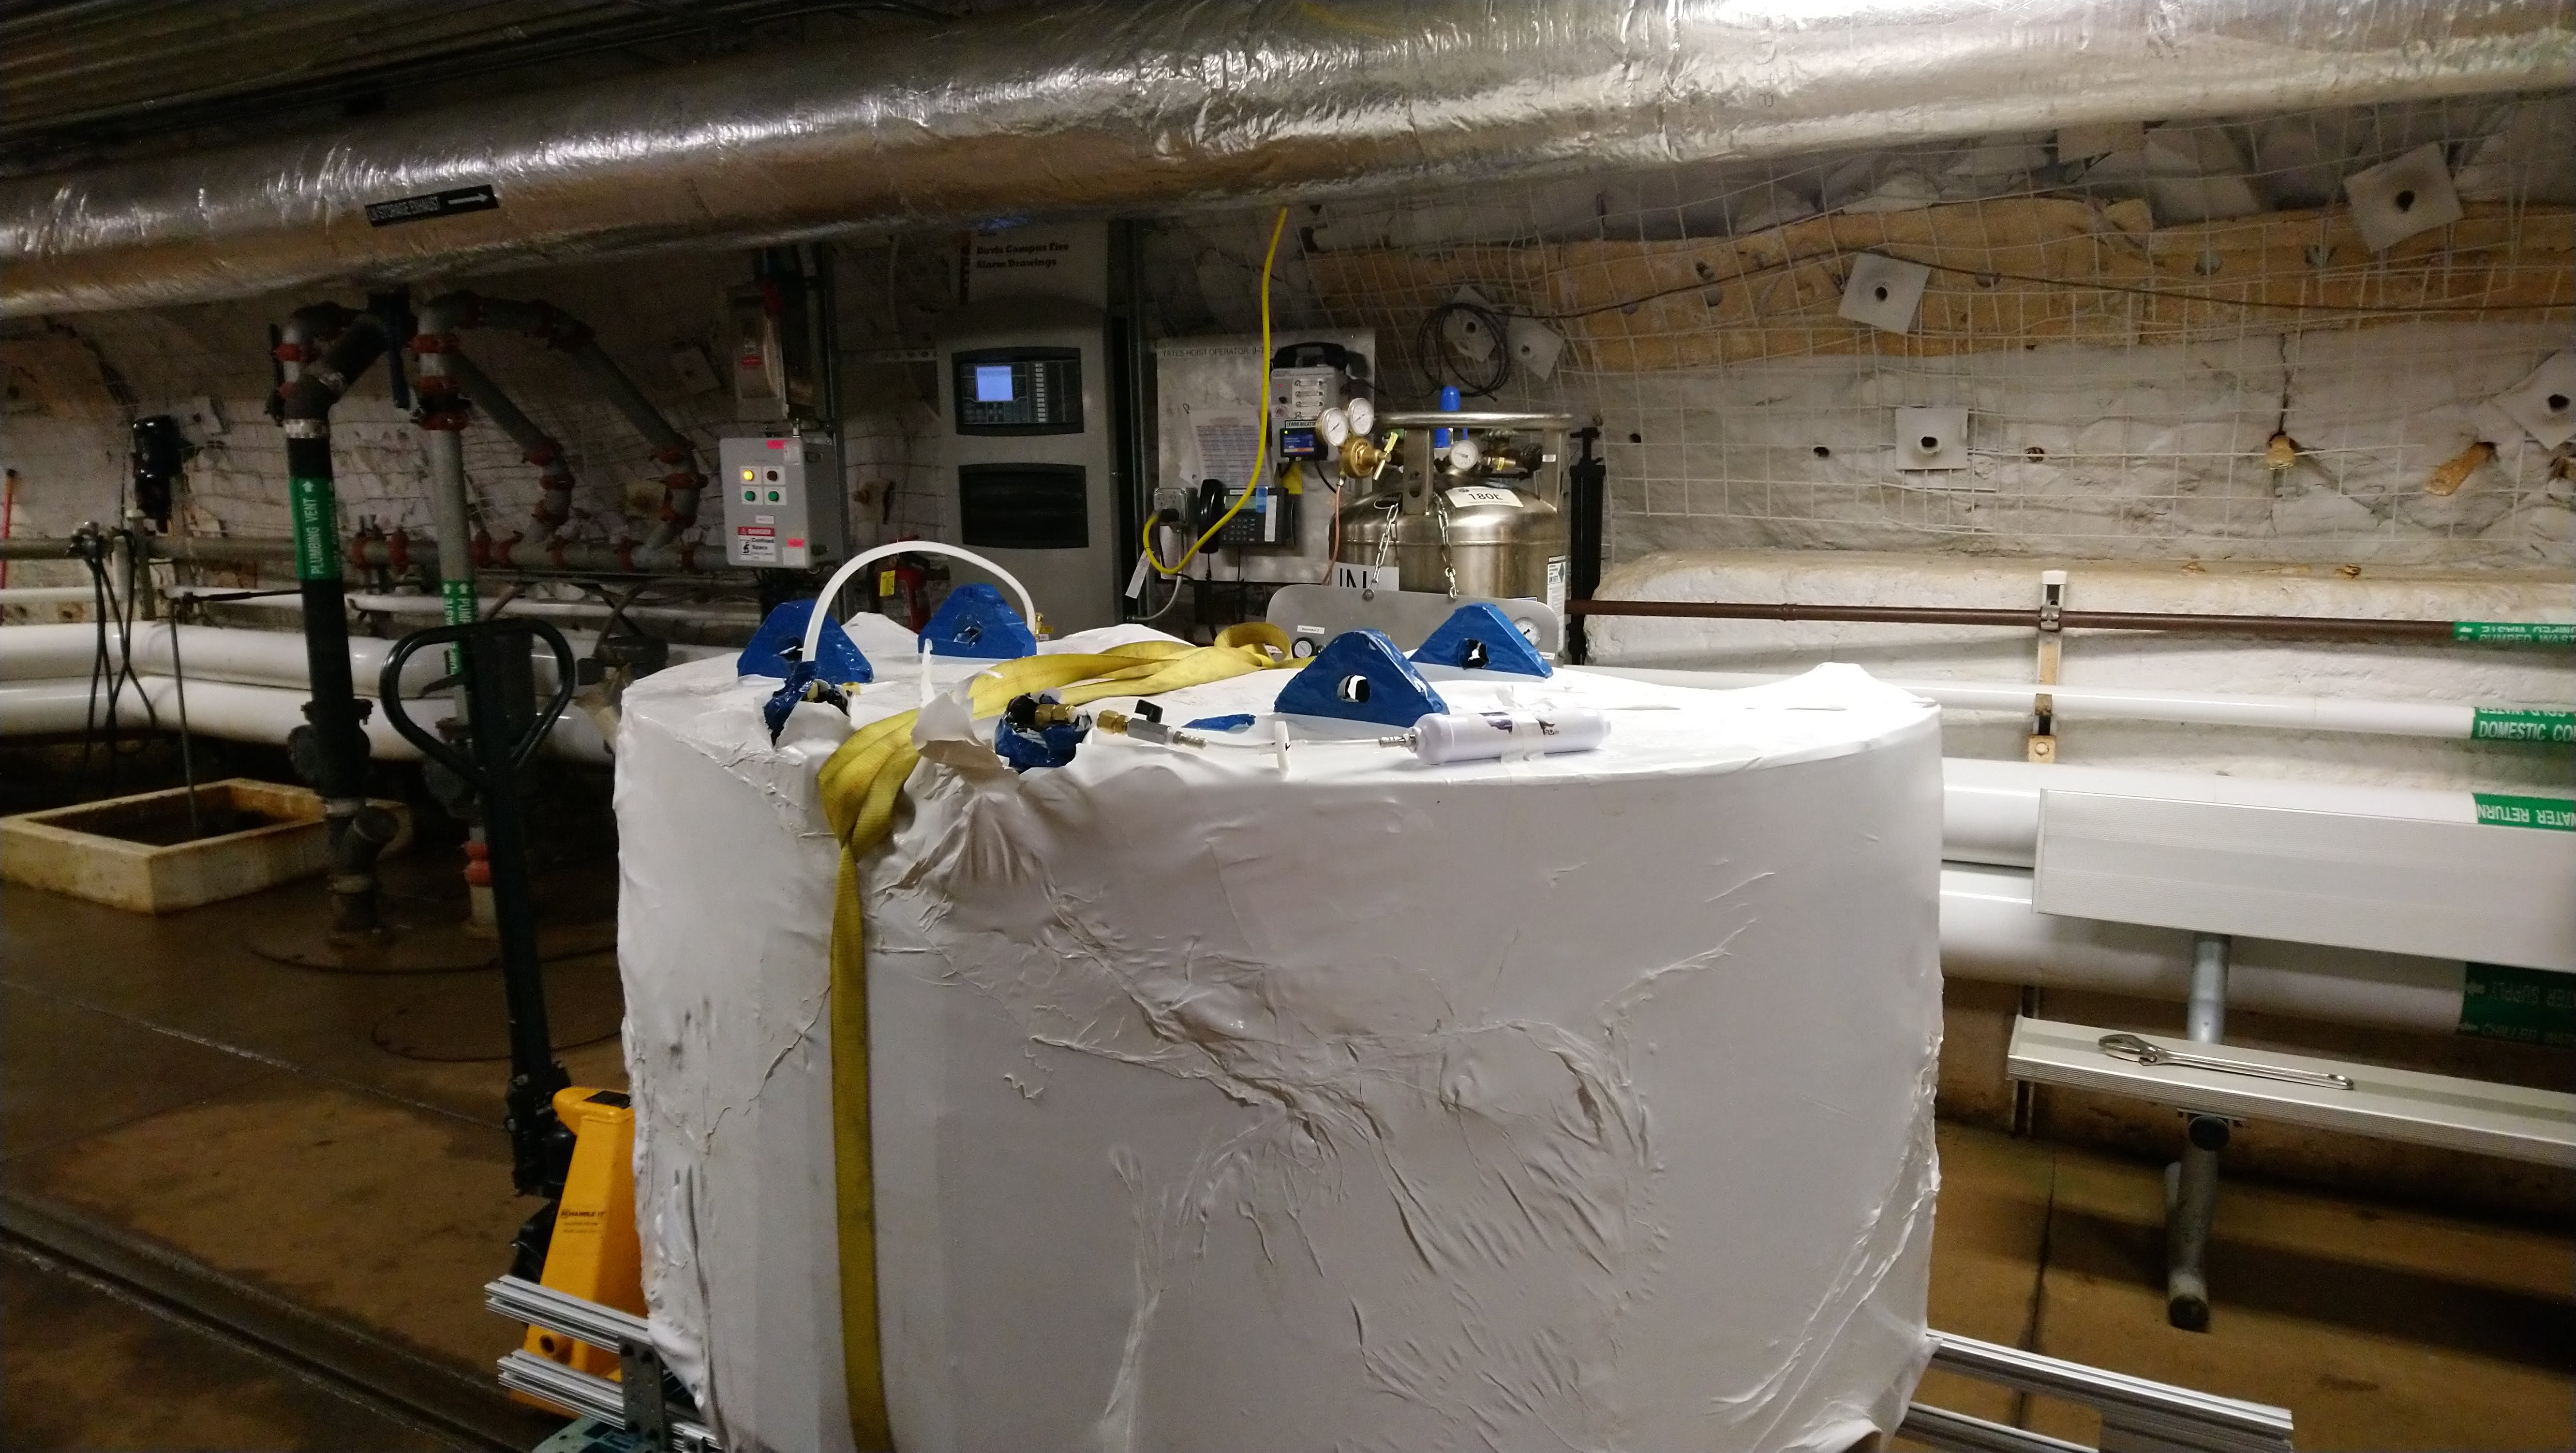
\includegraphics[width=\textwidth]{Figures/Construction/tat_purging.JPG}
\centering
\caption{Photograph of the a top tank setup for N2 purge.}
\label{fig:TAT_purging}
\end{figure}

\par
The proposed solution was to 'correct the curvature' with additional foam on top of the OCV, which due to construction delays and COVID-19, did not begin until August 2020.
The foam chosen for this was Styrodur\textsuperscript{\textregistered} \cite{styrodur_foam_ref}, chosen for having a high compression strength.
It also had the benefit of being onsite as it was already planned to be used around the side tanks and was assayed in \cite{LZ_assay_ref}, namely 
The primary bonding methods used to secure the foam to the OCV was HandiFoam\textsuperscript{\textregistered} \cite{handifoam_ref}.
HandiFoam\textsuperscript{\textregistered} was chosen as it securely held test pieces together, but also would fill in any potential gaps.
Additionally, the foam was held in place with titanium pins, and titanium rods.
Part of the installation is shown in \autoref{fig:TAT_foam_installation}.

\begin{figure}[!tbph]
\begin{subfigure}{.5\textwidth}
  \centering
  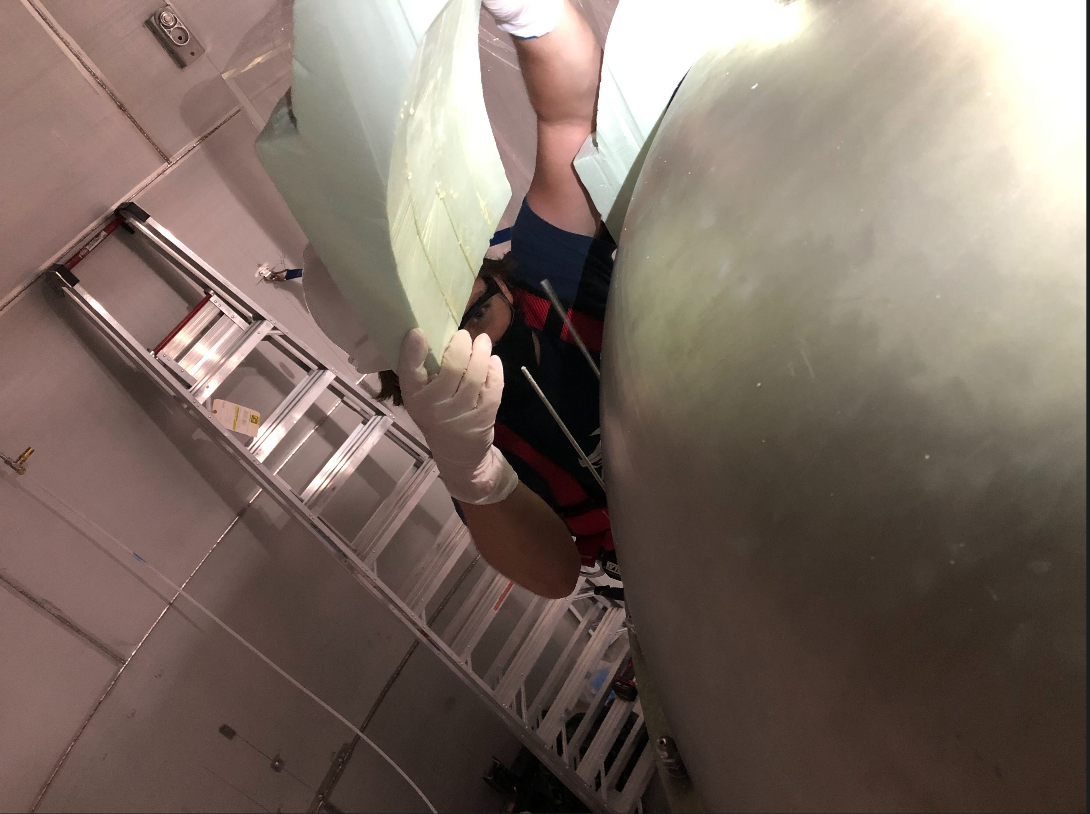
\includegraphics[height=6cm, width=\linewidth]{Figures/Construction/TAT_foam_installation.png}
  \end{subfigure}
  \begin{subfigure}{.5\textwidth}
  \centering
  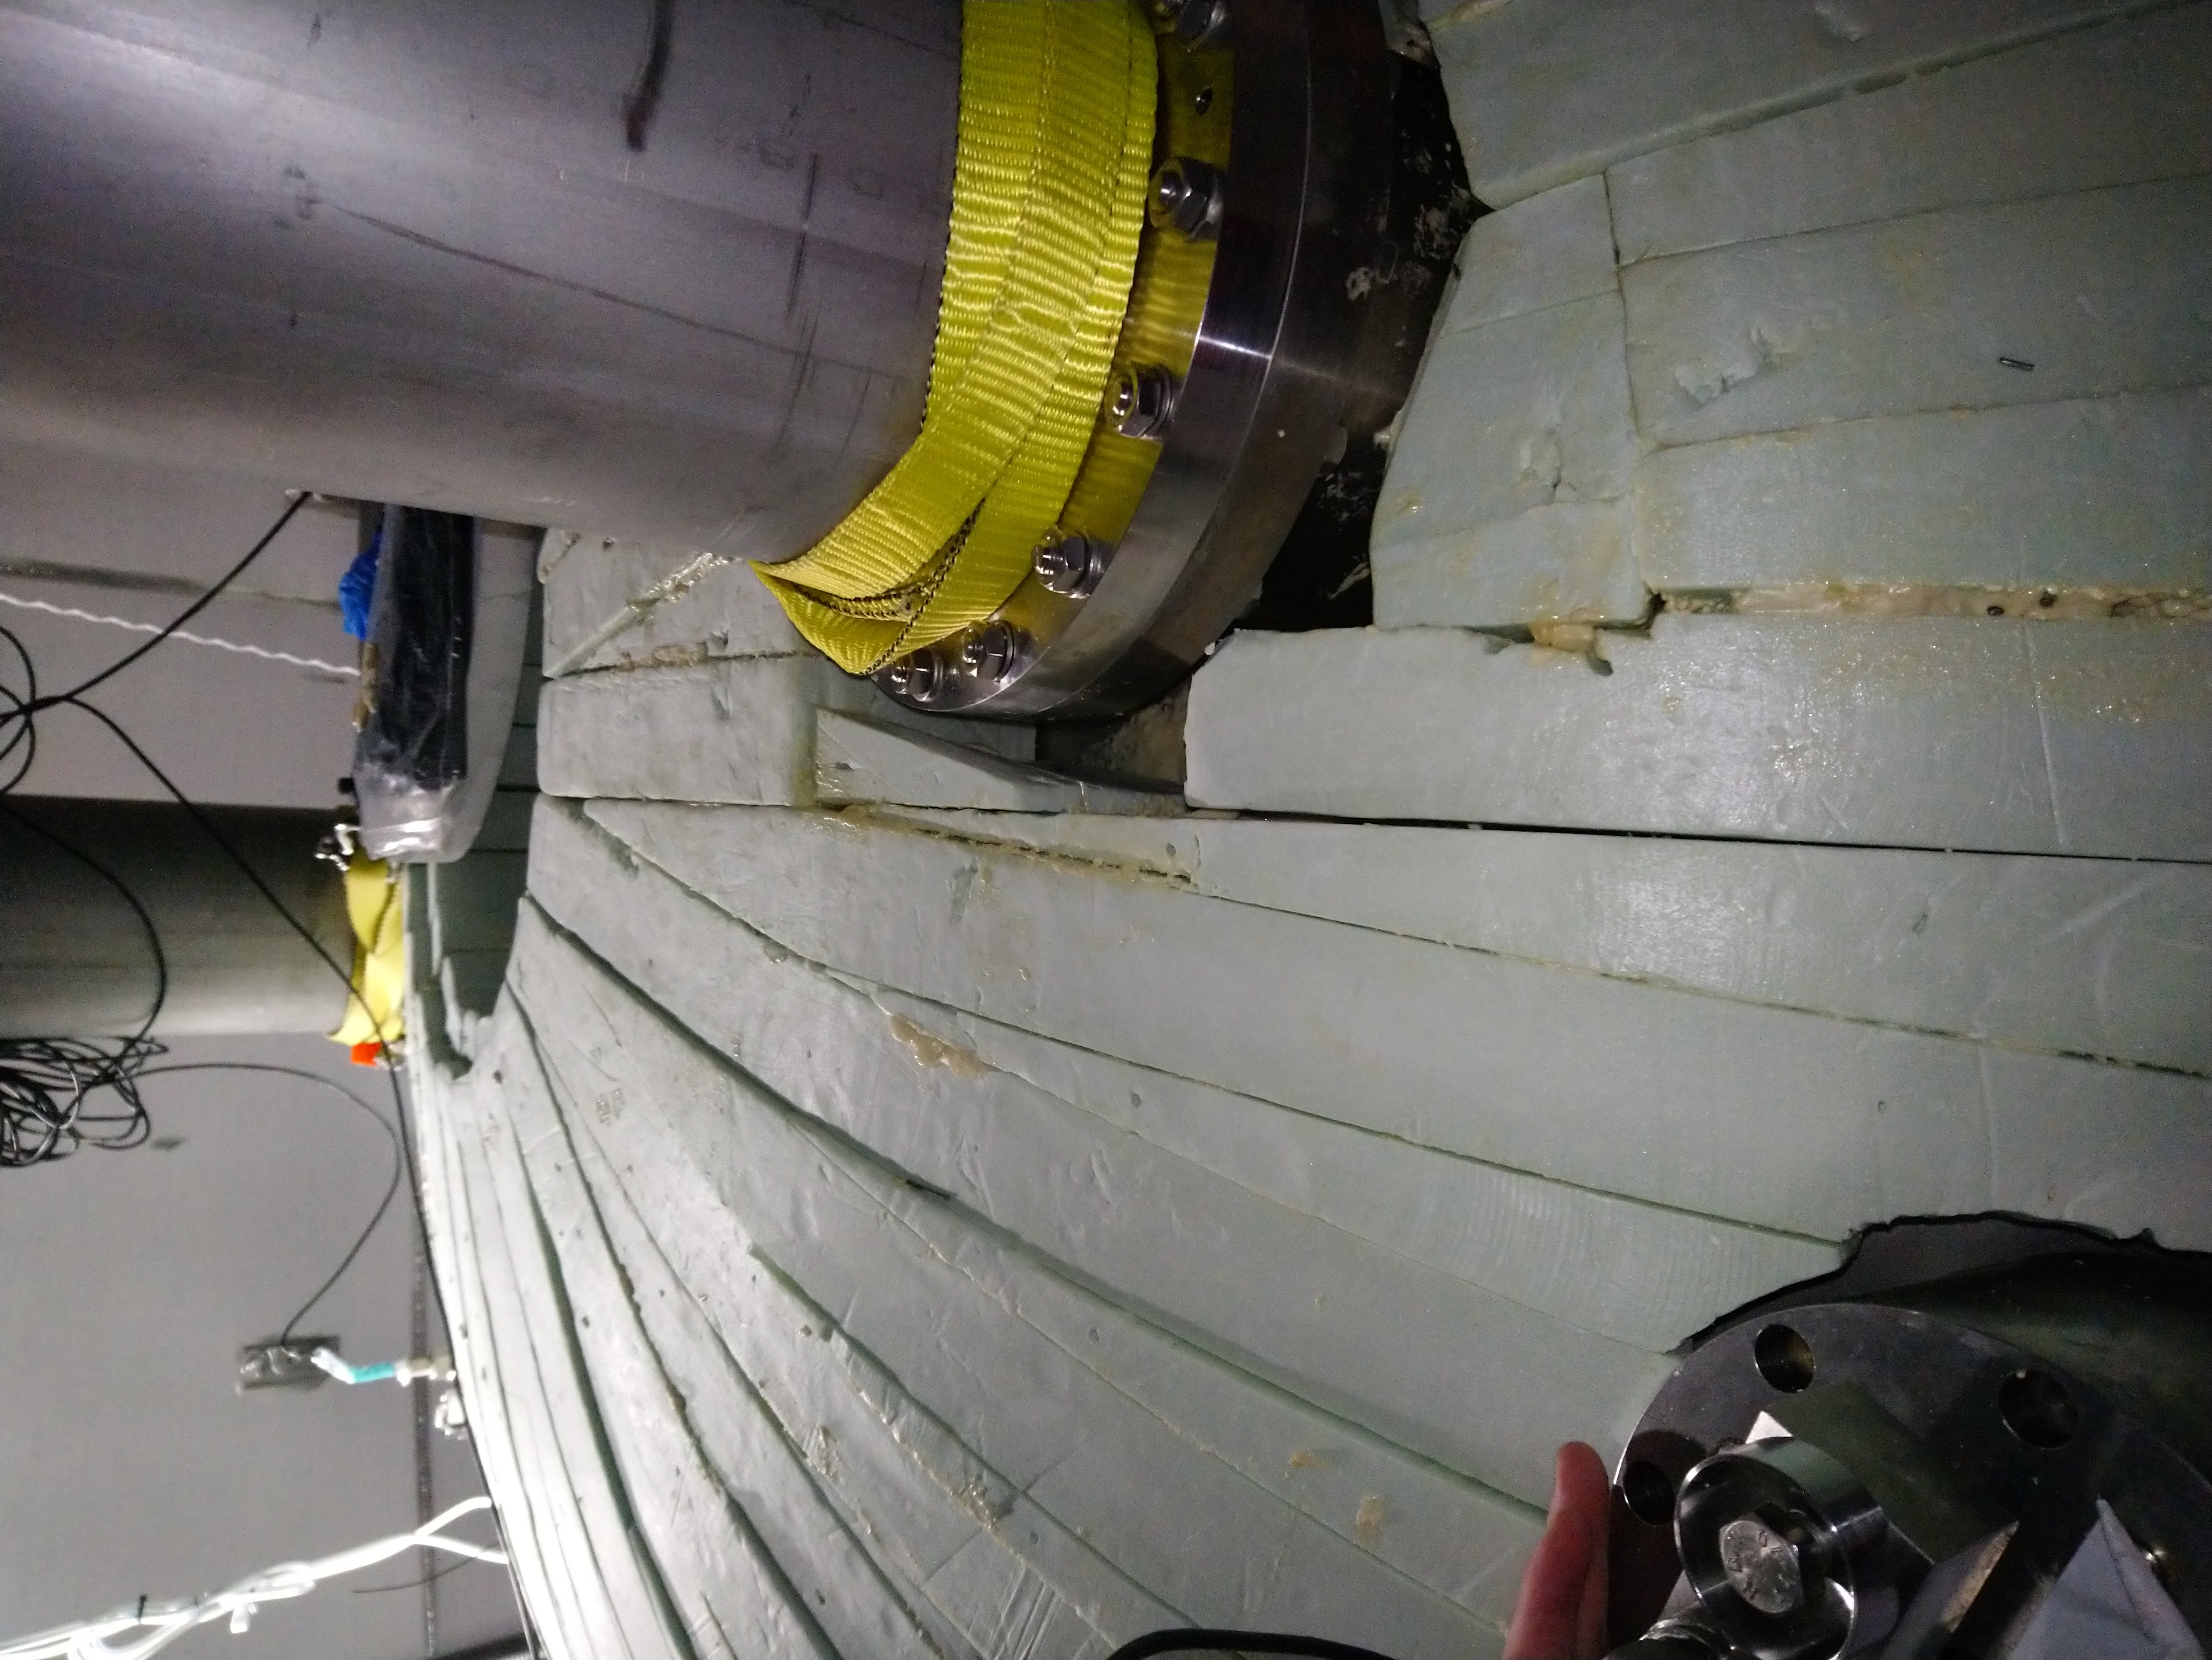
\includegraphics[height=4cm, width=6cm, angle=-90, width=\linewidth]{Figures/Construction/TAT_foam_complete.jpg}
  \end{subfigure}
\caption{Photograph of TAT-OCV foam installation.}
\label{fig:TAT_foam_installation}
\end{figure}

\par
The SAT-OCV foam was installed after the TAT-OCV foam in a slightly different fashion.
These pieces were primarily secured together using silicon sealant \cite{dowsil_silicone_ref} to each other and the OCV.
Titanium pins were also used to secure pieces together and trapping them behind the bolts on the OCV.
The final fit-test is shown in \autoref{fig:SAT_foam_guys}.

\par
As the foam had been underground for a number of weeks prior to being used, each piece of foam installed underwent a final `shaving', shown in \autoref{fig:foam_saving}.
A few mm was taken from each side of the foam to remove Radon chain particles that may have embedded themselves in the foam.

\begin{figure}[!tbph]
  \begin{subfigure}{.5\textwidth}
  \centering
  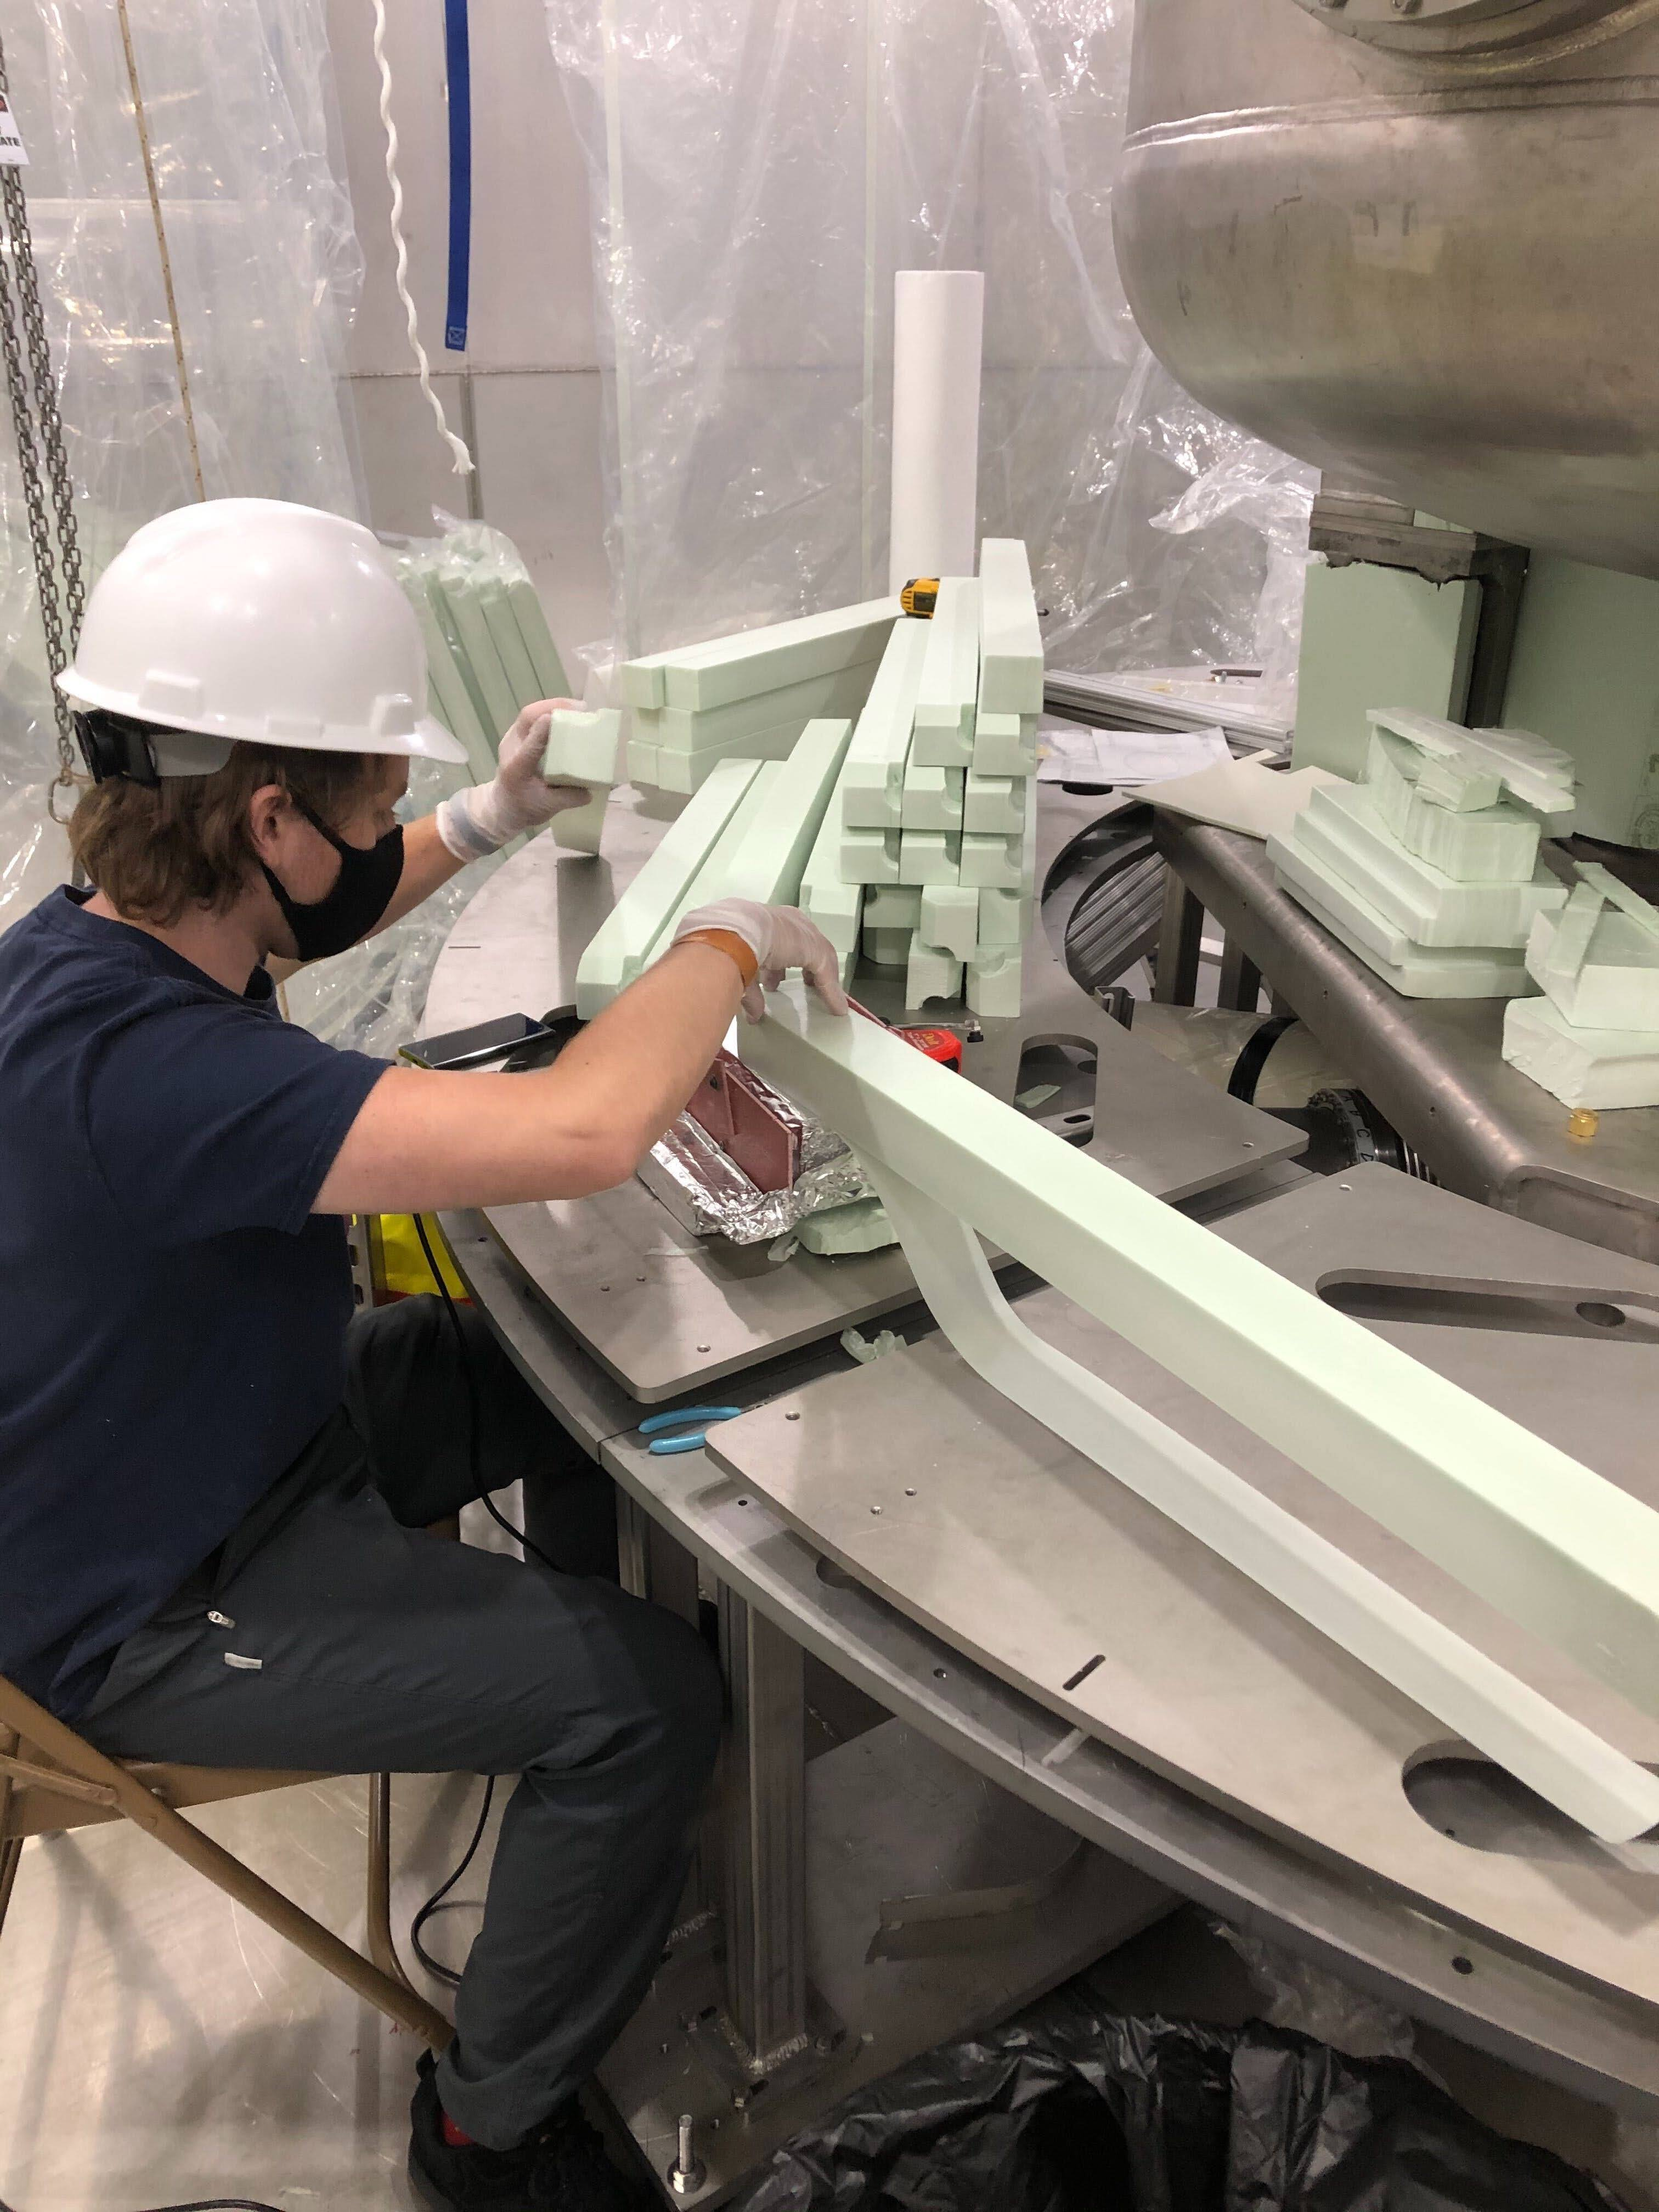
\includegraphics[width=\linewidth]{Figures/Construction/foam_shaving.jpg}
  \caption{Author using a hot-knife to shave all SAT foam prior to installation.}
  \label{fig:foam_saving}
  \end{subfigure}
  \begin{subfigure}{.5\textwidth}
  \centering
  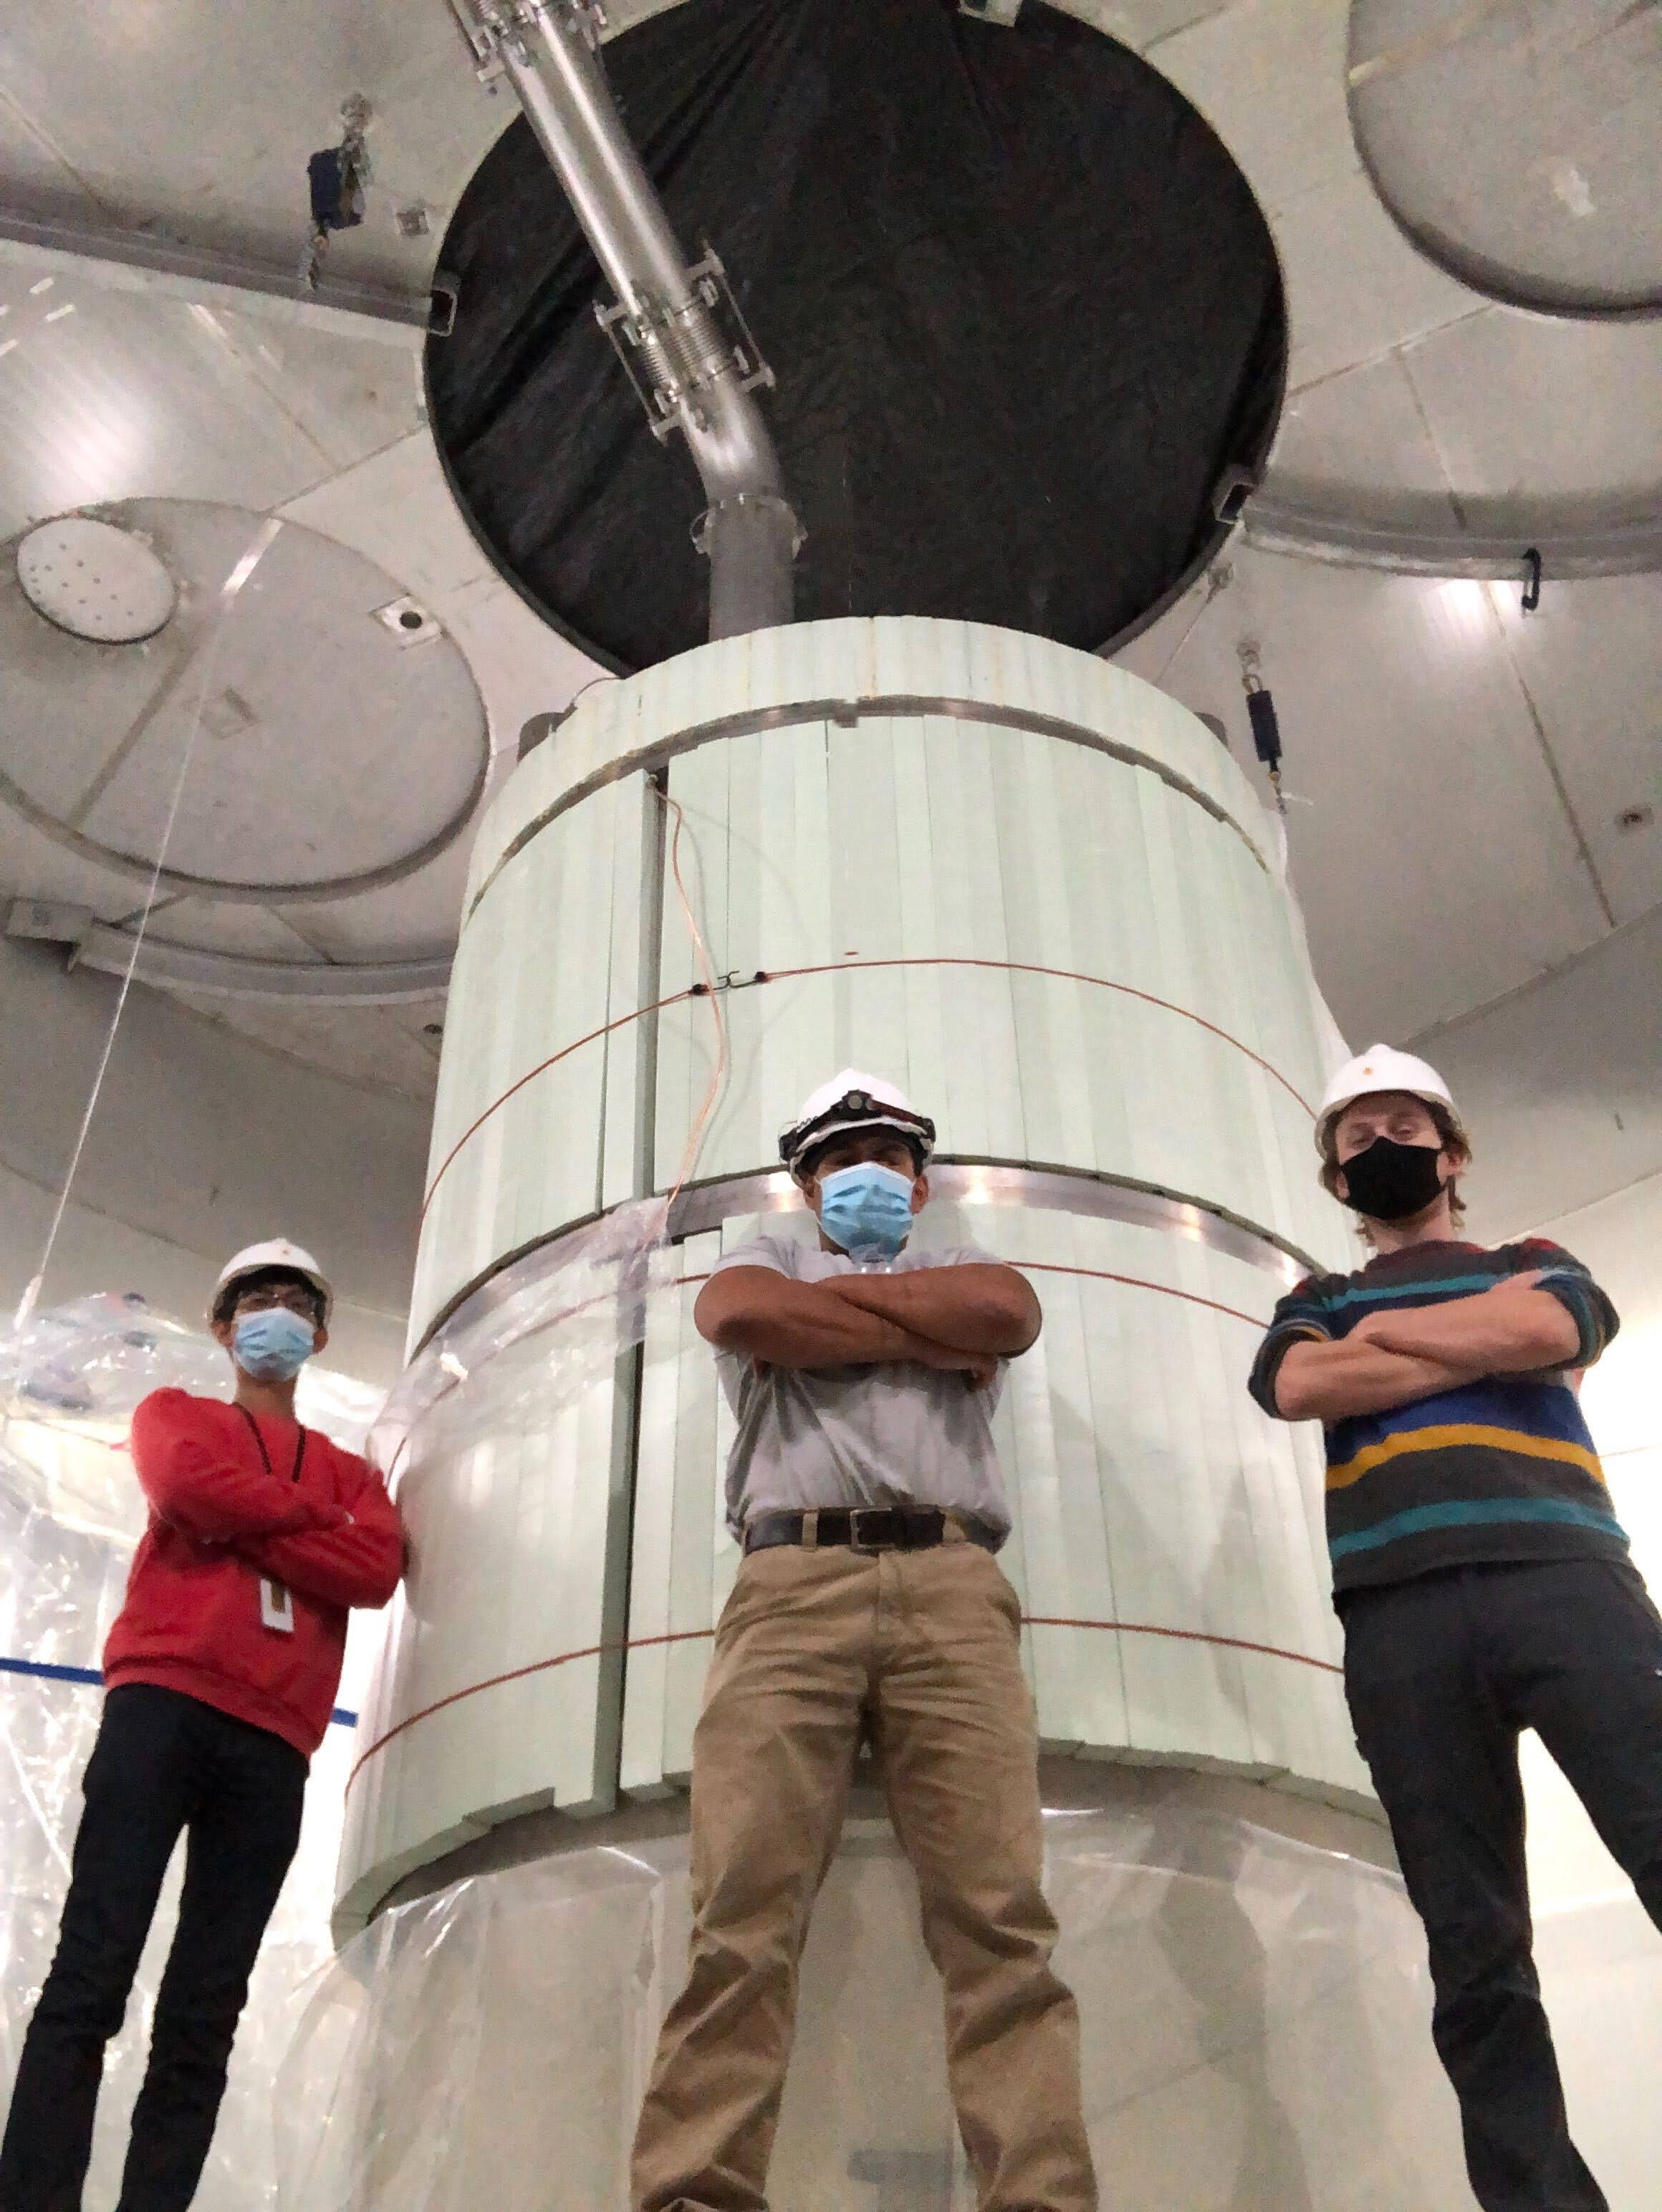
\includegraphics[width=\linewidth]{Figures/Construction/SAT_foam_fittest.jpg}
  \caption{OD installers Left to Right: Ryan Wang, Derek Lucero, Sam Eriksen}
  \label{fig:SAT_foam_guys}
  \end{subfigure}
\caption{Photographs of SAT-OCV foam installation.}
\label{fig:SAT_foam_installation}
\end{figure}

\par
Additional foam was installed around the OCV legs in between the BATs.
This foam was secured using HandiFoam\textsuperscript{\textregistered} as shown in \autoref{fig:ocv_leg_foam}.

\begin{figure}[!tbph]
\begin{subfigure}{.5\textwidth}
  \centering
  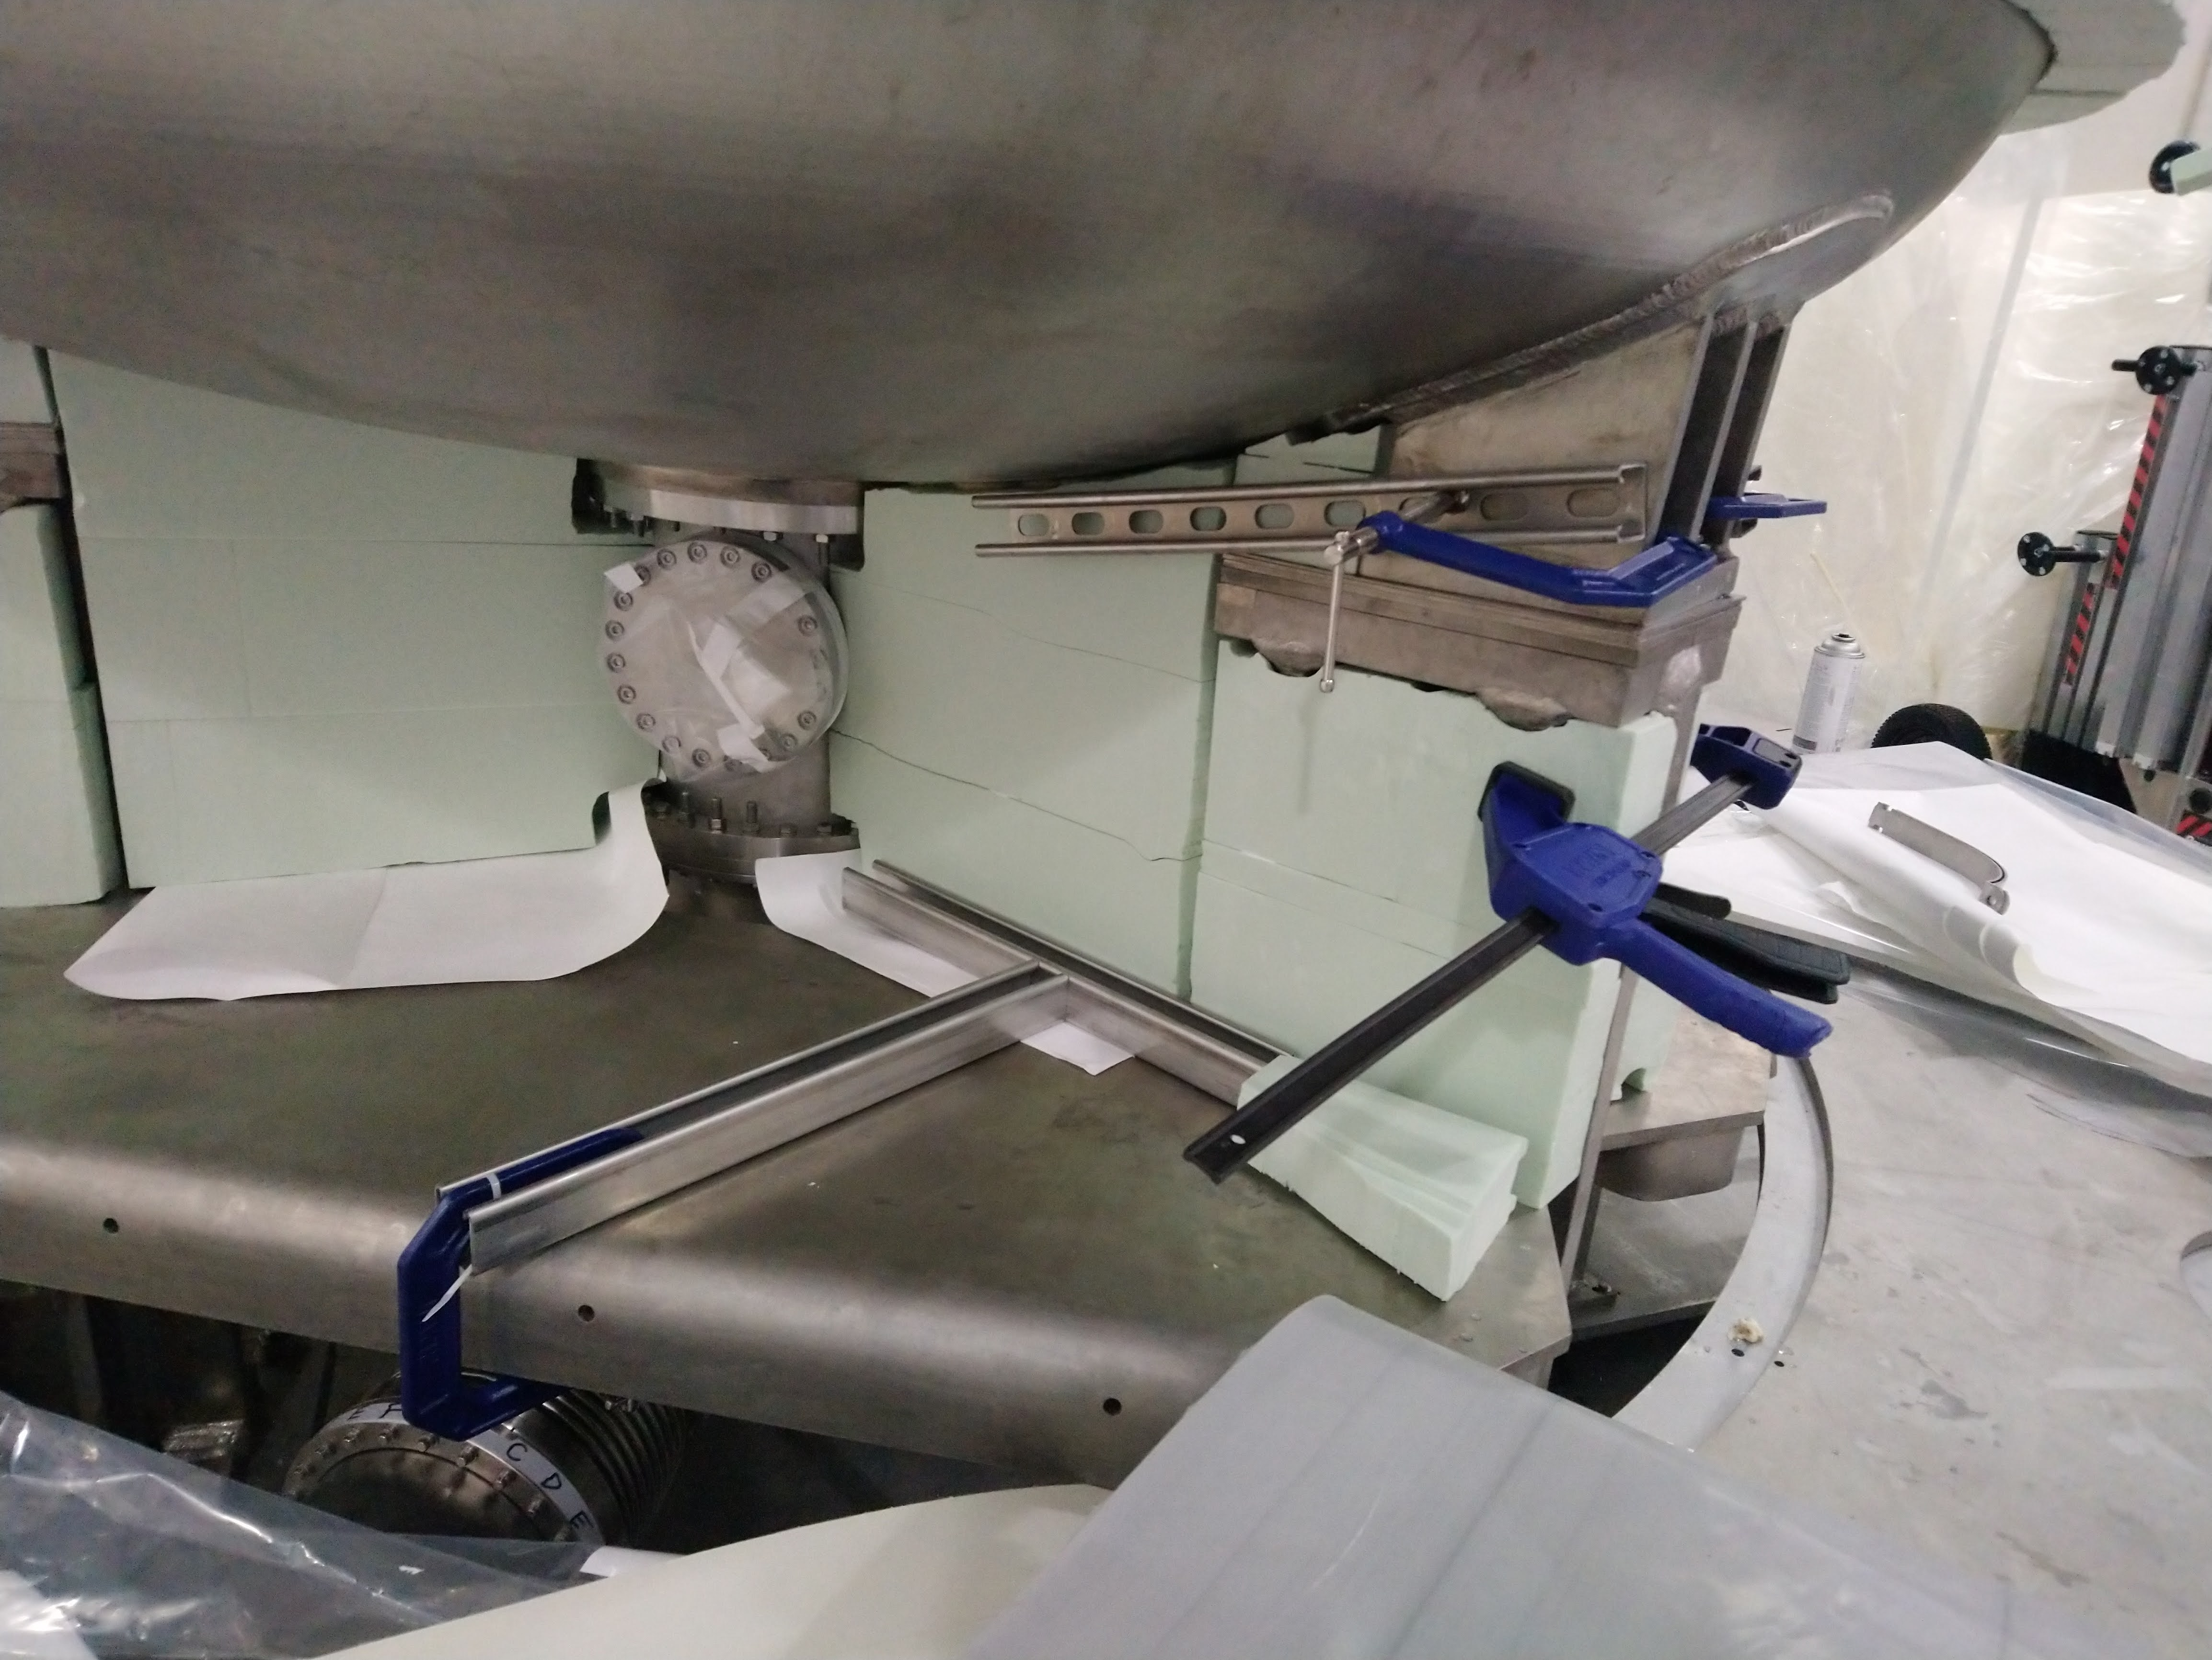
\includegraphics[height=6cm, width=\linewidth]{Figures/Construction/BAT_green_foam.JPG}
  \caption{OVV leg foam installation.}
  \label{fig:ocv_leg_foam}
  \end{subfigure}
  \begin{subfigure}{.5\textwidth}
  \centering
  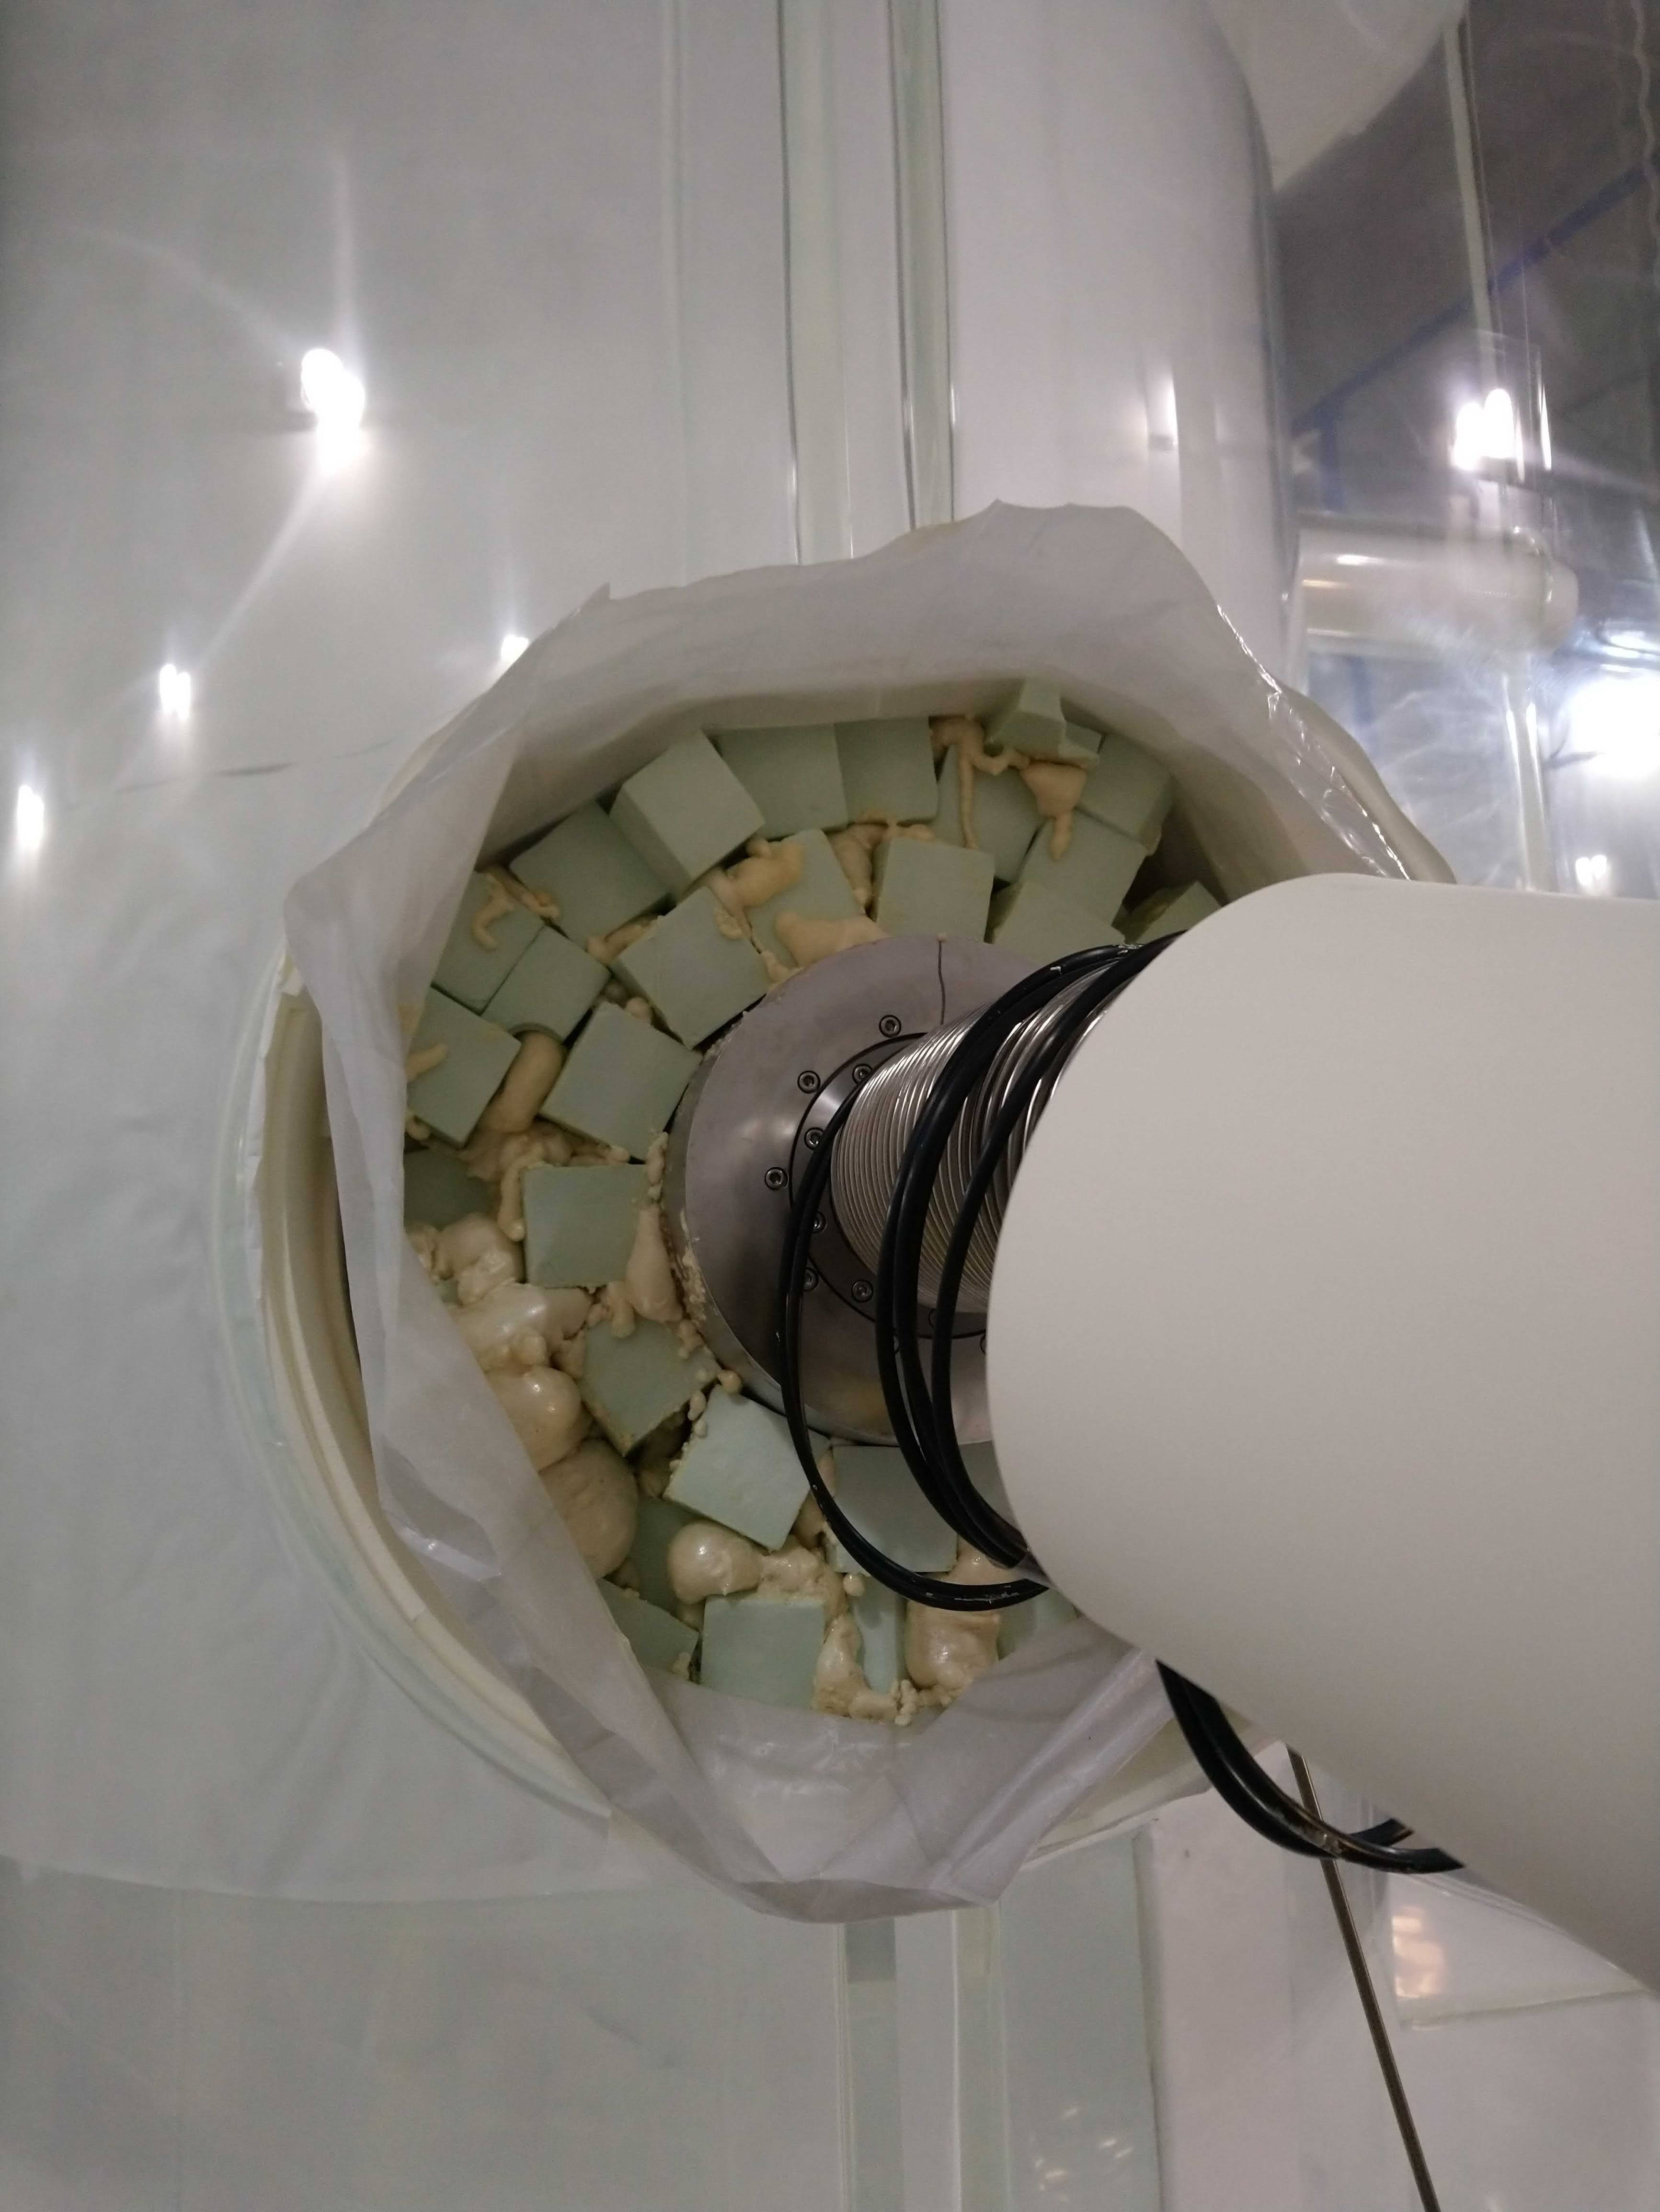
\includegraphics[height=6cm, width=\linewidth]{Figures/Construction/HV_foam.jpg}
  \caption{Foam installed around HV-feedthrough in SATs.}
  \label{fig:hv_port_foam}
  \end{subfigure}
\caption{Photographs of foam installed around OCV and HV-feedthrough.}
\label{fig:Additional_foam_installation}
\end{figure}

\par
Because of the aforementioned split tank and thin walls, there was a danger that the tanks may leak GdLS.
This is not necessarily a problem as GdLS is oil-based it would float to the top of the water, allowing it to be collected easily.
However it does not react well with either Tyvek or foam, both of which surround the OCV, and so any leaking GdLS would inevitably come into contact with them.
For Tyvek, over long exposure the optical reflectivity is damaged, reducing light collection in the OD, but would still work to some extent.
The foam on the other hand would degrade sufficient that it would not longer serve it's purpose as a water displacer after any contact.
As such, polyethylene sheets were installed to cover the foam.
On top of this, the Tyvek was installed.
In addition, the OD-Tyvek shape around the TAT was changed.
Previously this was a flat Tyvek sheet lying on top of the TAT and out to the OD PMTs.
However, in order to allow for a potential GdLS leak to reach the surface, a TeePee design was adopted.

\par
During the BAT test-fitting, it was found that these also did not match the curvature of the OCV.
Additionally, because of the placement of the securing feet underneath them, they were not stable.
This mean that as the water tank was filled, the BATs would be able to rock and bash into the OCV and potentially break their feet off.
The installation solution was to secure the BATs as much as possible with foam.
A different, thinner foam was selected for this purpose as a degree of flexibility was required to follow the OCV curve.
In this place 1/4-inch and 1/2-inch polyethylene foam were selected \cite{white_foam_ref}.
Additionally, HandiFoam\textsuperscript{\textregistered} was used for smaller places that could not be reached.
Neither of these foam solutions had been assayed.
The final BAT installation is shown in \autoref{fig:BAT_installation}.

\begin{figure}[!tbph]
\begin{subfigure}{.5\textwidth}
  \centering
  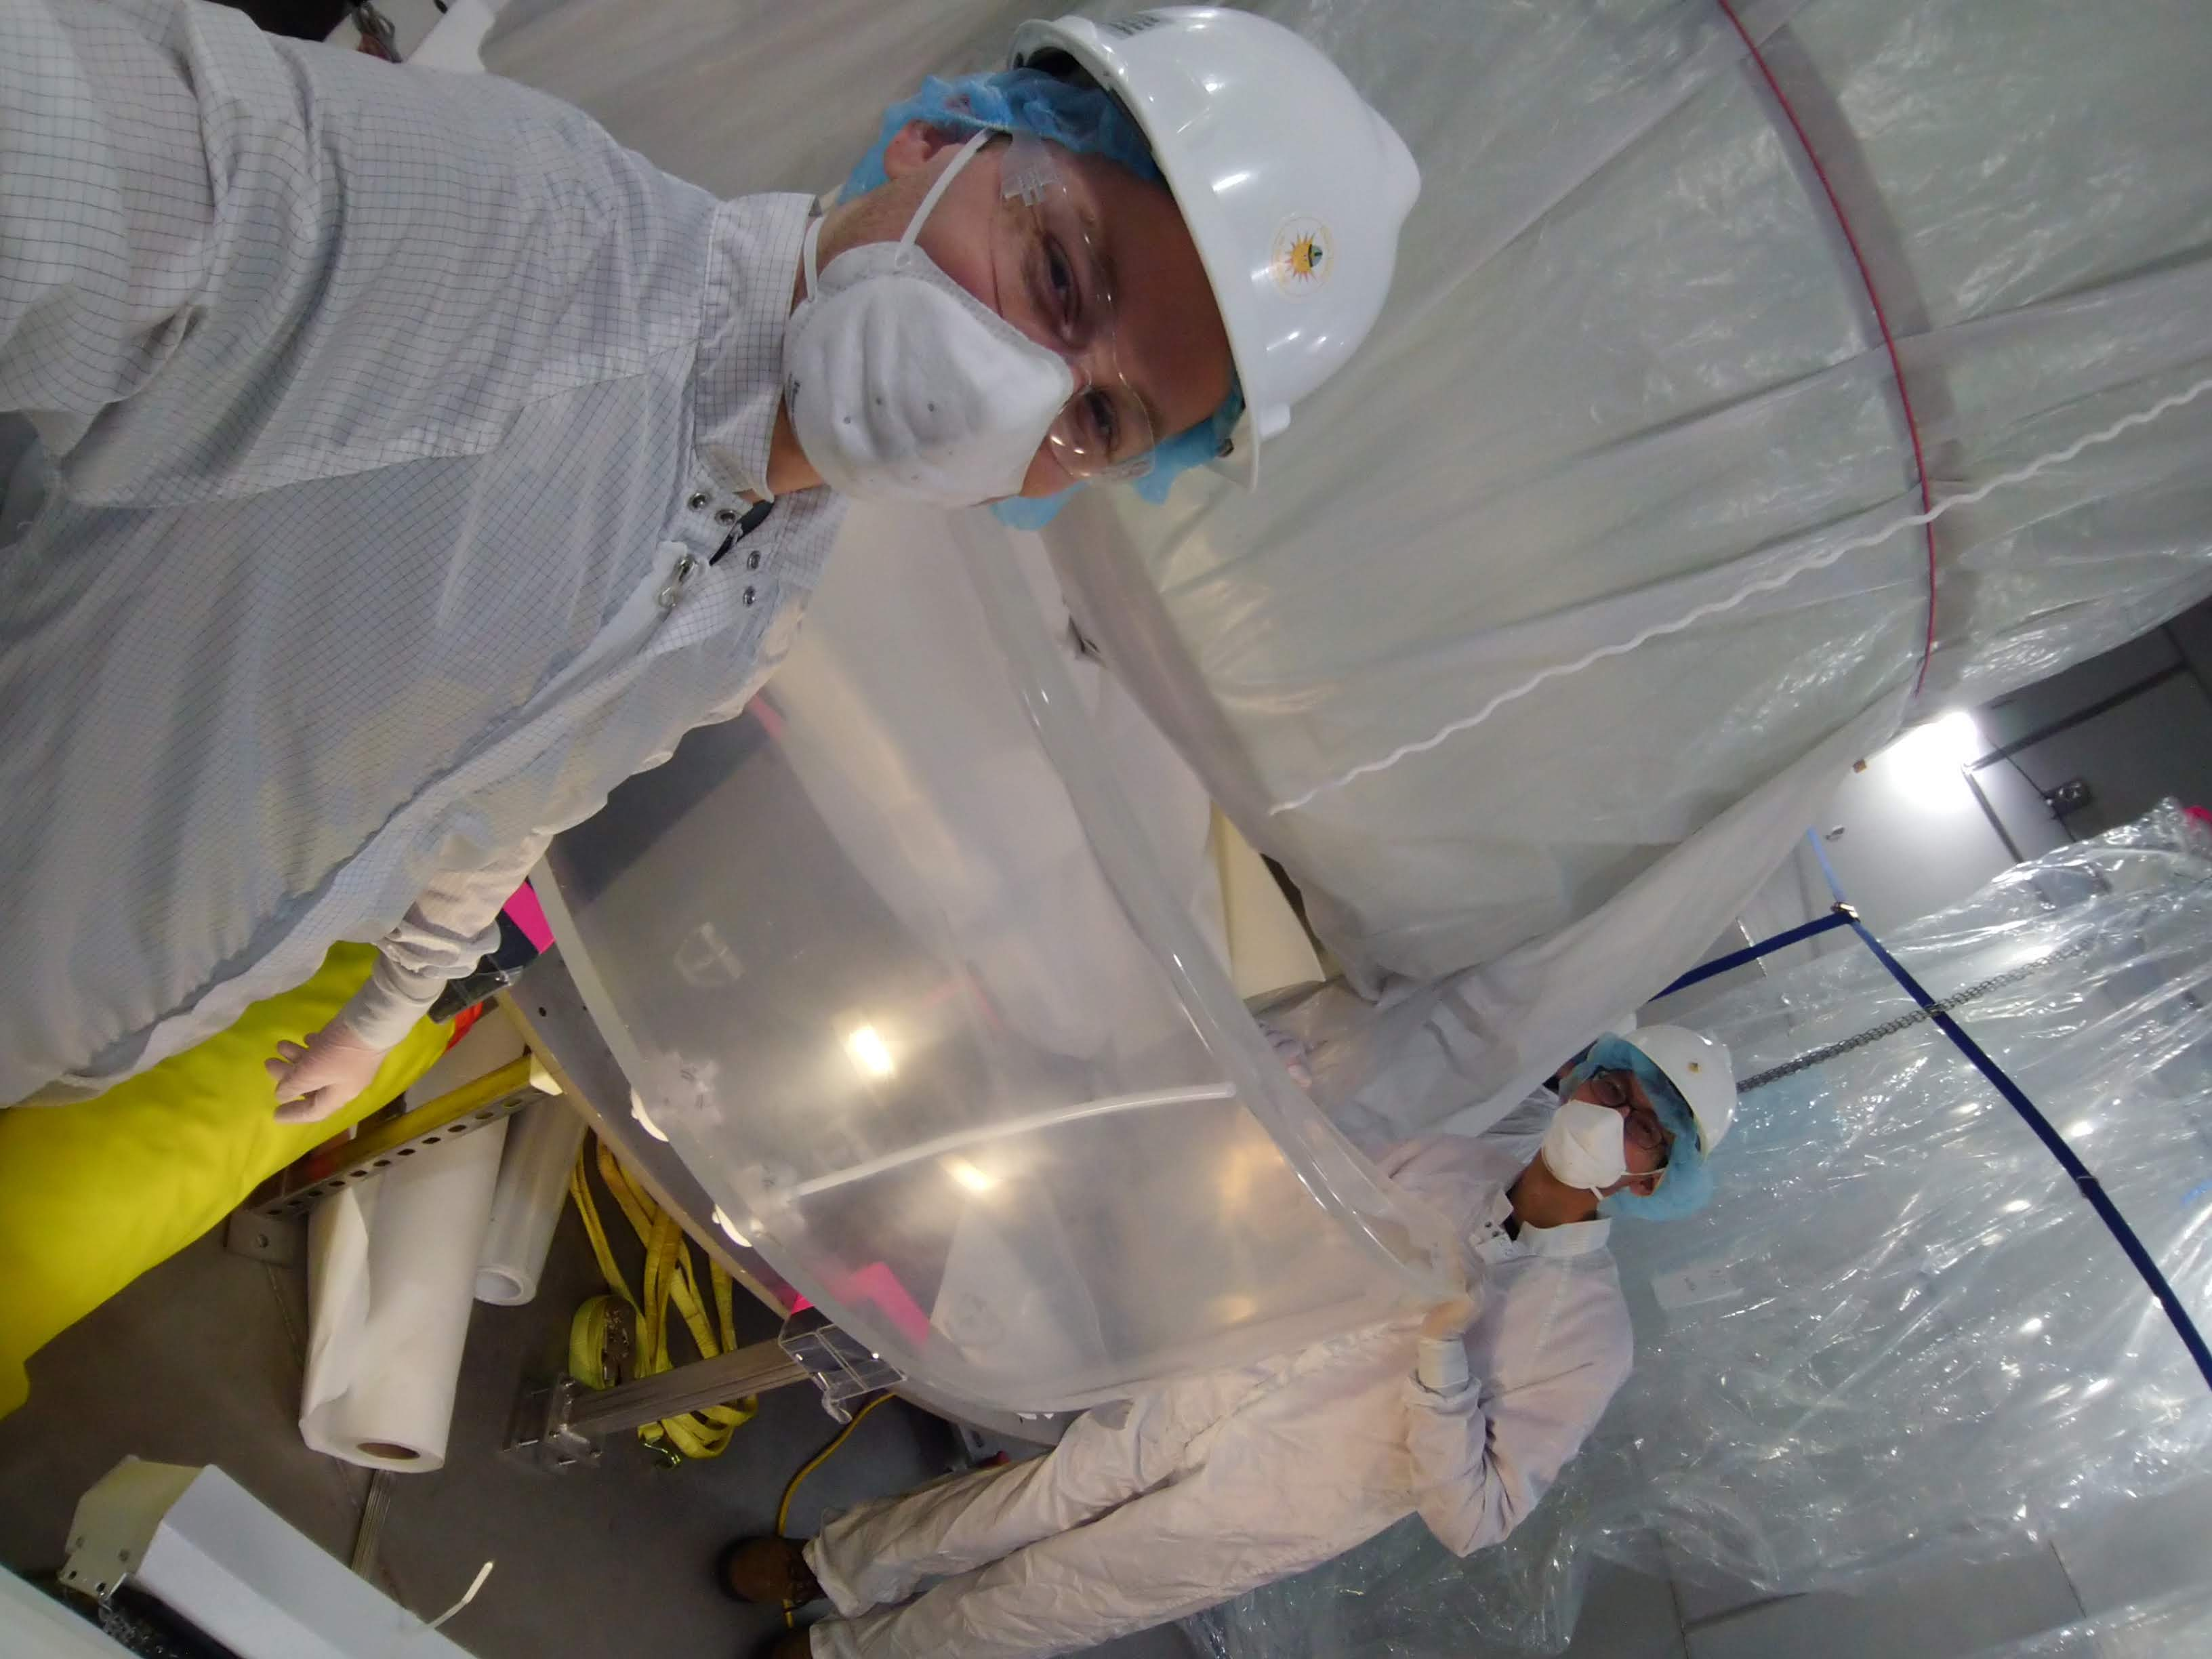
\includegraphics[angle=90, width=\linewidth]{Figures/Construction/BAT_installation.jpg}
  \caption{Installation of the final BAT}
  \label{fig:BAT_installation}
  \end{subfigure}
  \begin{subfigure}{.5\textwidth}
  \centering
  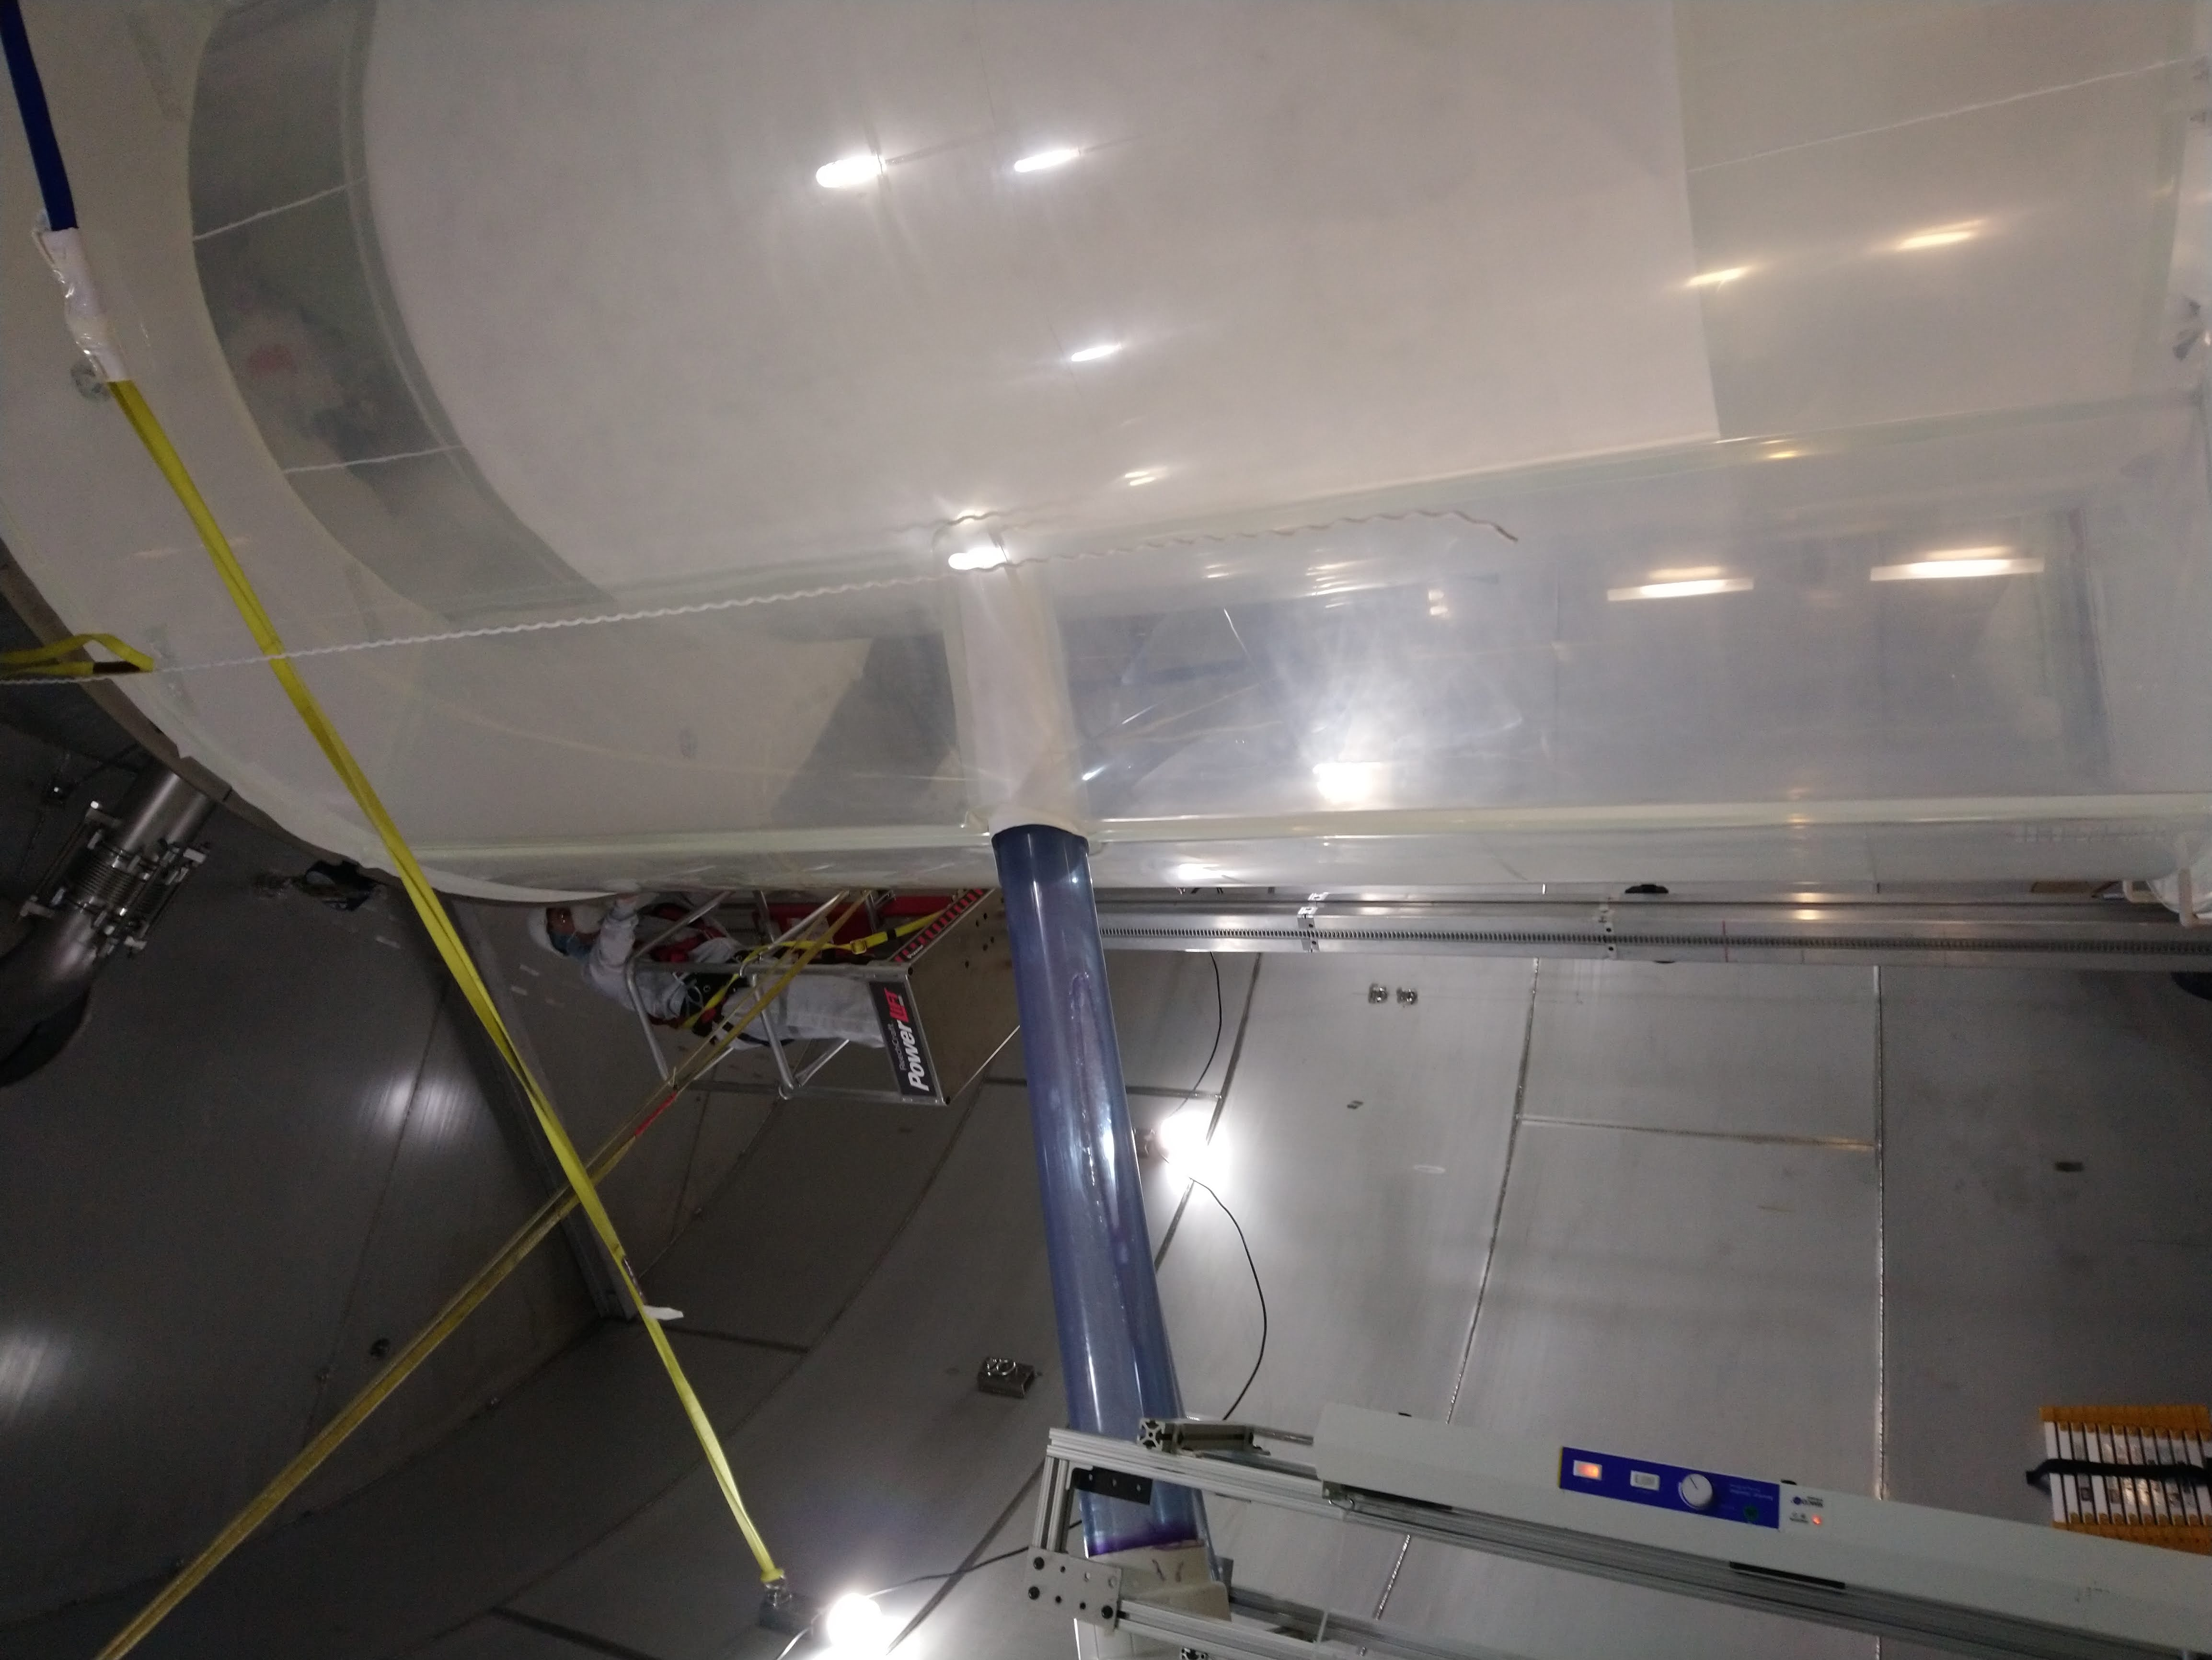
\includegraphics[angle=-90, width=\linewidth]{Figures/Construction/SAT_titanium_plate.JPG}
  \caption{Author securing the SAT.}
  \label{fig:SAT_titanium_installation}
  \end{subfigure}
\caption{Photographs of BAT and SAT installation.}
\label{fig:sat_and_bat_installation}
\end{figure}

\par
In additional to what has been mentioned, the SATs were secured using titanium plates.
To even the load the SATs experiences, 1-inch thick polyethylene foam was installed above and below.
Additional foam was installed and secured with HandiFoam\textsuperscript{\textregistered} around the High Voltage port, where previously this was just water.
This is shown in \autoref{fig:hv_port_foam}.

\par
The Tyvek was installed as single layers with excess overlapping.
The use of a single layer will have a performance reduction with the reflectivity reducing by $\approx$10\% compared to multiple layers bonded together \cite{tyvek_reflectivity_ref}.

\par
The culmination of this is the completed OD, shown in \autoref{fig:complete_od}.

\begin{figure}[!tbph]
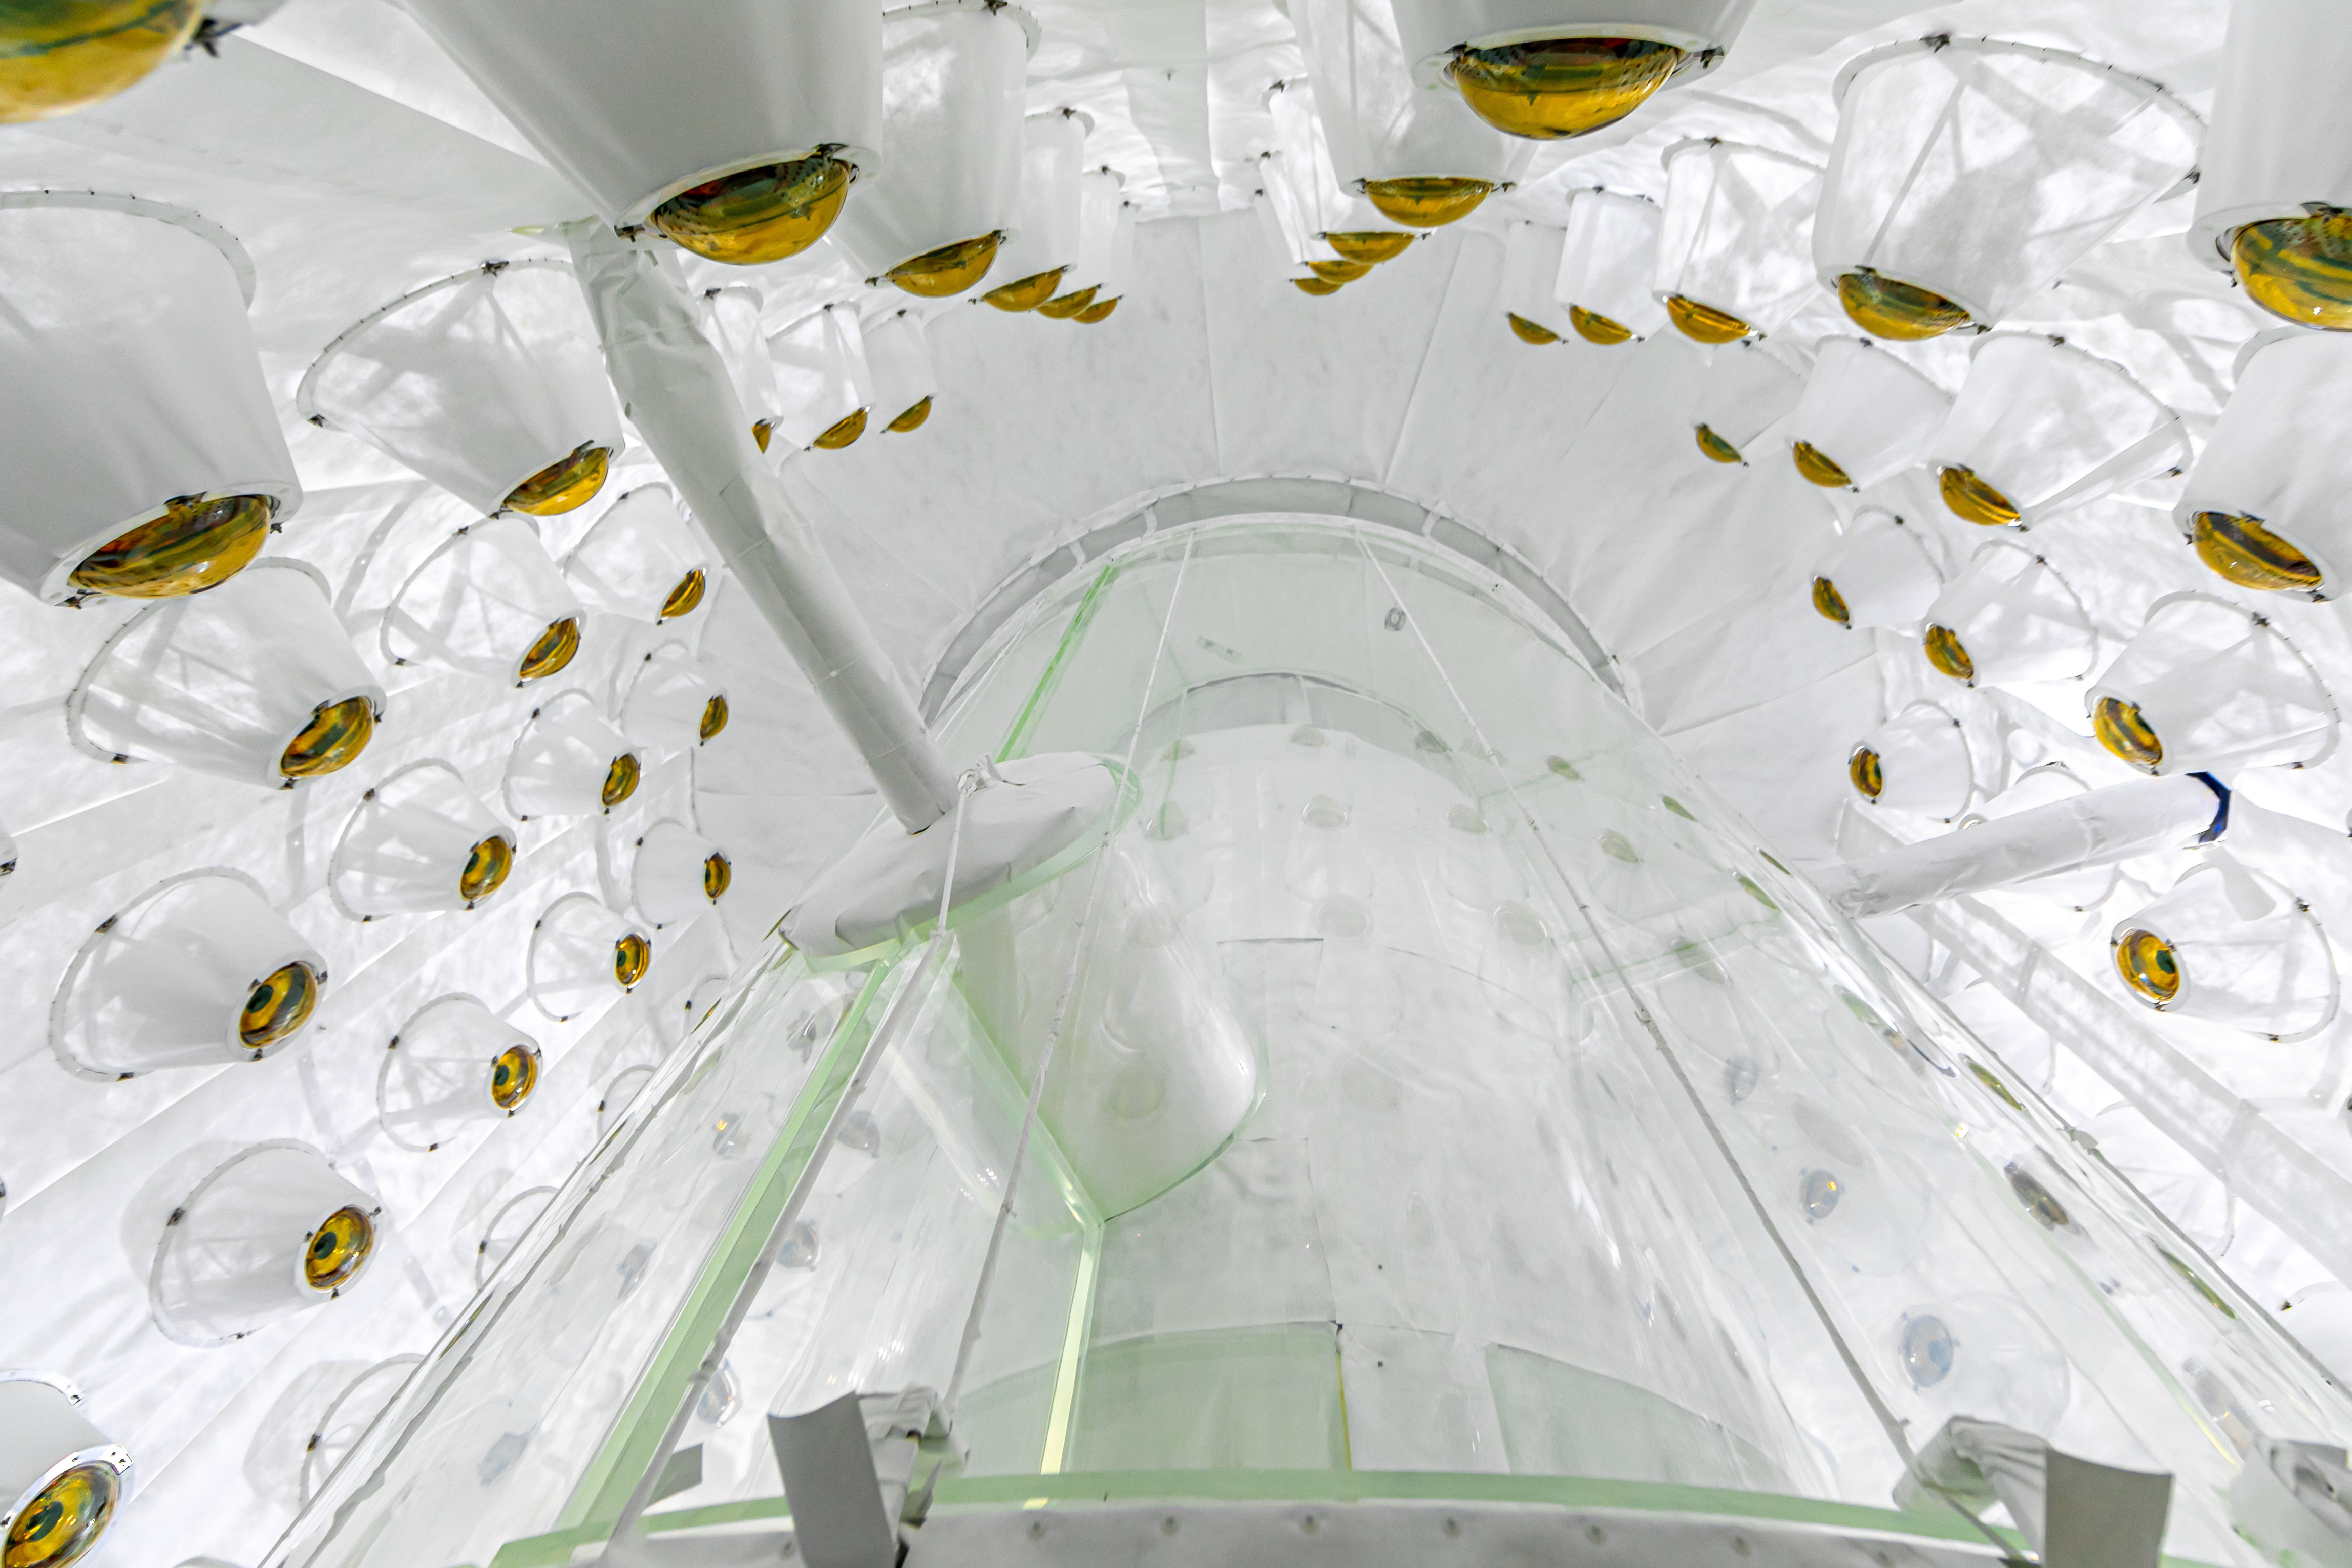
\includegraphics[width=\textwidth]{Figures/Construction/od_complete.jpg}
\centering
\caption{Completed OD installation}
\label{fig:complete_od}
\end{figure}

\par
During the installation described above, the blasting for the Deep Underground Neutrino Experiment (DUNE) began \cite{dune_blasting_ref}.
There was a concern that the pressure change caused by this would damage the tanks.
To stop this, the valves of the tanks were opened whenever there was a planned blast.
This left the inside of each tank open to the cavern-air during this time.

\subsection{Simulation Adaptation}
\par
Many of these design changes, whether it be material or geometrical will have some effect on the performance on the OD.
Most of the changes discussed above have been implemented in the simulation: the raised TATs, the additional foam and the Tyvek TeePee.
Other differences such as the acrylic tank thickness have now been propagated into the simulation.
What is implemented within the simulation can be seen \autoref{fig:Geometry_Differences} where the differences between design as as-built are highlighted.


\begin{figure}[!tbph]
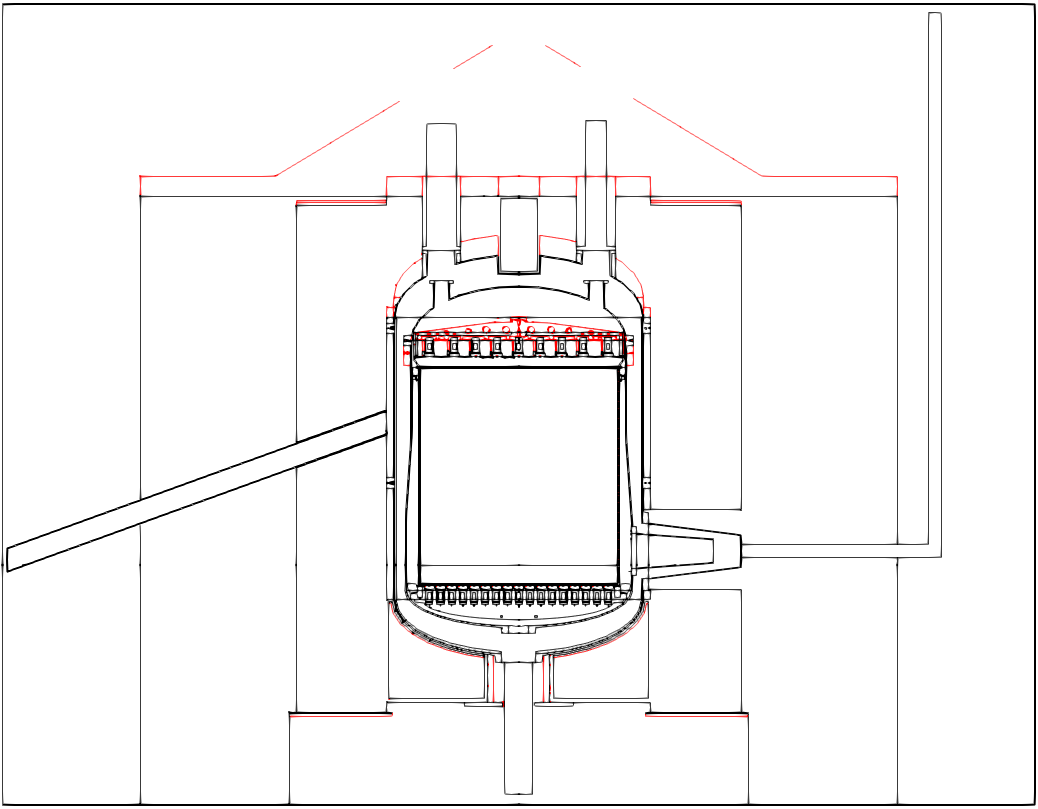
\includegraphics[width=\textwidth]{Figures/Geometry/geometry_differences_black_and_white.png}
\centering
\caption{LZ geometry slice as implemented in Geant4 from the water tank in. In black: the designed geometry as in \autoref{fig:LZ_Cut_CAD}. In Red: changes to the design including raised Top OD tanks and additional foam. OD PMTs are not shown here due to none lying on this plane.}
\label{fig:Geometry_Differences}
\end{figure}


%\begin{table}[!htbp]
%    \centering
%    \begin{tabular}{ c | c | c } 
%    \hline
%    \multirow{2}{*}{Volume} & \multicolumn{2}{l}{Percentage captured in volume (\%)} \\ 
%                            & All Neutrons  & SS and FID  \\ \hline
%    volA    & 0.0   & 1232\\
%    volB    & 0.0   &
%    \end{tabular}
%    \caption{Fraction of background neutrons captured in various detector volumes}
%    \label{tab:fraction_of_neutrons_captured_in_volumes}
%\end{table} 

\section{OD performance requirements}
\label{sec:simulated_od_requirements}
\par
As previously stated, the primary purpose of the OD is to act as an active veto for neutrons.
Practically, this means that there are a number of performance requirements which the OD has to meet, all of which can be found in \cite{LZ_TechnicalDesignReview_ref}.
A subset, which are addressed in this thesis are presented in \autoref{tab:veto_requirements}.
\begin{table}[!htbp]
    \centering
    \begin{tabular}{p{0.3\textwidth}p{0.6\textwidth}} %{ c | c {\textwidth} } 
    \hline
    {Requirement Number} & {Description} \\ \hline
    R-160001             & Detection efficiency of 95\% for a 1 MeV neutron that scatters once in the xenon \\
    R-160005             & Must not veto more than 5\% of the WIMP search live-time
    \end{tabular}
    \caption{Selection of the OD veto performance requirements. Adapted from Table 12.2.6 from \cite{LZ_TechnicalDesignReview_ref}}
    \label{tab:veto_requirements}
\end{table} 
R-160001 is defined for a 1 MeV neutron as that is the most likely neutron energy expected in the TPC (more on this later).
R-160005 is set to a 5\% impact so as to not reduce the exposure (and therefore discovery potential) of LZ too much.

\par
The veto method adopted by LZ is to act as a `dumb' veto, as no attempt will be made to determine the cause of light seen in the OD.
This means that a single scatter event in the TPC will be vetoed if, in that event there is a signal see in the OD which:
\begin{enumerate}
    \item has energy above some threshold.
    \item is within some time window of the scatter in the TPC. 
\end{enumerate}
The veto window and threshold are determined by the background rate in the OD in order to reduce the impact on live-time.
This does however need to be balanced to maintain a suitable veto efficiency, as not all neutron captures in the OD will result in high energy signals.
These are both explored in the remainder of this chapter.

\subsection{OD Backgrounds}
\label{sec:simulated_od_backgrounds}
\par
A background in the OD is any event that is not what it was designed to detect and veto - so any event that is not a neutron or $\gamma$ that has scattered once in the TPC.
There have been numerous pre-construction studies to determine the expected background rate in the OD including \cite{LZ_TechnicalDesignReview_ref,LZ_projected_sensitivity_paper_ref,sallyshaw_thesis_ref,scotthaselschwardt_thesis_ref,lz_od_taup_2019_ref}, with the expected rate varying wildly, from between 56 Hz and 230 Hz above 200 keV.
In order to make sense of it, the key backgrounds are explained here and a expected rate in the OD is determined based upon the lastest information about the detector.

\subsubsection{GdLS impurities}
\par
As part of the radioassay for LZ discussed previously, a dedicated campaign was undertaken to determine the rate of backgrounds in the GdLS \cite{scotthaselschwardt_thesis_ref}.
This LS screener campaign was motivated by the need to measure the $^{14}$C rate, a low $\beta$-decay (156.5 keV) which would essentially set what the minimum veto energy threshold could be.
If the rate of $^{14}$C is too high and the veto energy threshold set too low, then a large portion of TPC events would be vetoed mistakenly.
In \cite{LZ_TechnicalDesignReview_ref}, the proposed veto energy threshold was 100 keV.
The radioassay also considered various decay chains and rare metals, both measured via $\alpha$ decays.
\par
One of the key discoveries of the screener campaign was the high ${}^{235}U$ rate, with the measured level far higher than the relative abundance of ${}^{235}U$ to ${}^{238}U$ would suggest (0.720\% and 99.274\% respectively), though is a feature seen in other experiments \cite{javierperez_thesis_ref,superkamiokande_neutron_tagging_ref}.
This prompted the decay chains to be probed as sub-chains of the full chain.
The full decay chains considered ($^{232}$Th, $^{235}$U and $^{238}$U) are shown in \autoref{fig:decay_chains} along with how the sub-chains were defined.
The results from the LS screener campaign are shown in \autoref{tab:gdls_assay_rates}.
\par
In comparing the non-doped LS to doped LS it was deduced that many of the contaminants were introduced as part of the purification of the Gd that occurs as it is added to the LS \cite{scotthaselschwardt_thesis_ref}.
As such, the method of doping the LS was altered, which aimed to reduce the contamination.
This `improved purification' GdLS is what was used to fill the LZ OD.
Included in \autoref{tab:gdls_assay_rates} are estimates from \cite{scotthaselschwardt_thesis_ref} of how this change in purification method will affect the GdLS, but it is important to stress that it did not undergo a radioassay, so the true rate is not known.
\par
The highest individual decay rate is from ${}^{14}$C.
This prompted a change in the veto energy threshold to be above the ${}^{14}$C end-point: 200 keV.
This value is then what has been used in sensitivity studies of LZ \cite{LZ_projected_sensitivity_paper_ref}.

\begin{table}[!htbp]
    \centering
    \begin{tabular}{c|c|c}
        \multirow{2}{*}{Isotope or Subchain}  &  \multicolumn{2}{c}{GdLS rates (mBq/kg)}      \\ 
                             &  LS Screener          & Improved Purification \\ \hline
        ${}^{238}U_{e}$      &  $< 1.04$             & $< 0.017$             \\ 
        ${}^{238}U_{m}$      &  $0.092\pm0.02$       & $0.010\pm0.004$       \\
        ${}^{235}U_{e}$      &  $0.011$              & $< 0.018$             \\
        ${}^{235}U_{l}$      &  $0.10\pm0.04$        & $< 0.012$             \\
        ${}^{232}Th_{e}$     &  $< 0.027$            & $< 0.0036$            \\
        ${}^{232}Th_{l}$     &  $< 0.020$            & $< 0.0030$            \\
        ${}^{40}K$           &  $< 0.22$             & $< 0.0092$            \\
        ${}^{138}La$         &  $< 0.0055$           & $< 0.0017$            \\
        ${}^{176}Lu$         &  $0.30\pm0.07$        & $0.0081\pm0.0018$     \\
        ${}^{152}{Gd}$       &  $1.61\pm0.08$        & $1.61\pm0.08$         \\
        ${}^{147}{Sm}$       &  $1.02\pm0.05$        & $1.02\pm0.05$         \\
        ${}^{14}{C}$         &  $4.77\pm0.098$       & $4.77\pm0.098$ 
    \end{tabular}
    \caption{Activities of GdLS components during LS Screener testing and those projected from an improved purification technique. Values from Table 4.9 and 6.11 of \cite{scotthaselschwardt_thesis_ref}}
    \label{tab:gdls_assay_rates}
\end{table}
\par
Another source that was measured in the GdLS radioassay was ${}^{7}Be$, with an activity of <2.69 \cite{scotthaselschwardt_thesis_ref}.
This has been purposefully ignored in \autoref{tab:gdls_assay_rates} as ${}^{7}Be$ has a half-life of 50-days \cite{be7_decay_ref}.
Therefore it will not be a significant contributor to the OD rate a year after the GdLS cocktail is created.

\input{Chapters/OuterDetector/Figures/decay_chains}


\subsubsection{Cavern-$\gamma$'s}
\par
Another outcome of the LS Screener campaign was the requirement for a dedicated Cavern-$\gamma$ study which was mentioned in \autoref{sec:cavern_gamma_generator}.
The Cavern-$\gamma$ study has already been discussed in \autoref{sec:cavern_gamma_generator} with the expected rates shown in \autoref{tab:cavern_gamma_generator_parameters}.
It showed that the rate of these $\gamma$s were 50\% lower than was what was anticipated in the Technical Design Review \cite{LZ_TechnicalDesignReview_ref}.
\par
One thing which wasn't included in that study however was the possibility of a fluctuation in the rate.
In \autoref{sec:cavern_gamma_generator} it is was assumed that all of the decays originate from the walls of the cavern.
This is not strictly true, as their is radon in the air which will contribute some amount to the $\gamma$ rate.
This can be caused by seasonal changes in the air flow within the mine, feature documented in other mines \cite{finnish_mine_radon_ref,nepal_mine_radon_ref,minos_annual_modulation_ref}.
In the most extreme cases, such as from the Soudan Underground Laboratory \cite{cavern_gammas_in_Soudan_mine_ref} there could be as much as a 26\% fluctuation in the rate.

\subsubsection{LZ Detector Components}
\par
A third source are decays originate from the detector components, all of which are contaminated with trace radioimpurities.
All of these were subject to an assay \cite{LZ_assay_ref}.
Although a lot of these decays result in particles with low penetrating power, there is a quantity which will reach the GdLS, though it is biased by proximity to the GdLS.
It was shown in \cite{scotthaselschwardt_thesis_ref} that the detector components can contribute as much as 11.9 Hz to the OD rate above 200 keV with the majority (5.5Hz) from the acrylic tanks and associated support structure.
\autoref{tab:gdls_non_assayed_activities} contains the activities of the components that are in closest proximity to the GdLS and were installed as part of the installation described in \autoref{sec:od_construction_sec}.
The mass estimates of soft materials are the author's own, based upon measurements and logs taken whilst on-site.

\begin{table}[!htbp]
    \centering
    \begin{tabular}{c|c|c|c|c|c|c|c}
        \multirow{2}{*}{Material or Component} & \multirow{2}{*}{Mass (kg)} & \multicolumn{6}{c}{Measured Activity (mBq/kg)}      \\ 
                    &        & ${}^{238}U_{e}$ & ${}^{238}U_{l}$ & ${}^{232}Th_{e}$ & ${}^{232}Th_{l}$ & ${}^{60}Co$ & ${}^{40}K$ \\ \hline
        HandiFoam\textsuperscript{\textregistered}   & 7 & 123 & 51 & 31 & 21 & 0 & 62 \\
        Fir tree Rivets                              & 2  & 52  & 14 & 6  & 8  & 0 & 18 \\
        3M 2216 Epoxy Adhesive                       & 0.1 & 7102 & 5325 & 26725 & 32111 & 0 & 2779 \\
        Dowsil 795 silicone sealant                  & 4   & 2120 & 2294 & 243   & 238   & 0 & 720 \\
        Tyvek                                        & 70  & 8  & 15  & 22     & 0     & 0 & 1330 \\
        OCV                                          & 1020 & 0.11 & 0.04 & 0.03  & 0.02  & 0.1 & 0.16 \\
        polypropylene sheets                         & 3   & 14.0 & 6.90 & 7.9  & 1.8  & 0 & 38.0 \\
        Styrodur foam                                & 40   & 20.0 & 57.0 & 2.60 & 9.0  & 6.0 & 80 \\ 
        White polyethyene foam                       & 15   & 120 & 12    & 22   & 13   & 0   & 105 \\
        SAT titanium plates                          & 308  & 0.11 & 0.04 & 0.03  & 0.02  & 0 & 0.16 \\
        Acrylic Tanks                                & 3140  & 0.0284 & 0.0284 & 0.0244 & 0.0244 & 0 & 2.3 \\
        Neutron conduits                             & 130  & 0.27 & 0.16 & 0.04 & 0.04 & 0 & 0.4 \\
    \end{tabular}
    \caption{Activities of components in close proximity to the GdLS. The activities are from \cite{LZ_assay_ref}
            Each material activity is given to the 68\% confidence level.}
    \label{tab:gdls_non_assayed_activities}
\end{table}

\par
In addition to the measurements in \autoref{tab:gdls_non_assayed_activities}, the OCV was subject to the cavern air for a prolonged period of time so there may be a build up of Radon dust which is not taken into account.
Similarly, the frequent opening of the valves on the OD tanks (as mentioned in \autoref{sec:cavern_gamma_generator}) will have allowed for cavern-air and dust to enter the tanks.
Quantifying this will not be possible without damaging the tanks, but it may be an unexpected feature in data.

\subsubsection{Expected Rate}
\par
All of the backgrounds discussed in this section were simulated with the `as build' detector geometry.
For the GdLS internal decays, the improved purification case was considered.
The simulations performed were energy deposits only, so no light collection efficiency or detection efficiency have been taken into account.
The rates observed in the OD above a number of energies is shown in \autoref{tab:od_expected_rates}.

\par
An interesting result of this is that with the improved purification of the GdLS, it may be possible for the veto threshold to be reduced to 100 keV.
This is because a rate <100 Hz is required for a 500 $\mu$s veto time window for a less than 5\% impact on WIMP-search livetime, and is what was planned for in \cite{LZ_TechnicalDesignReview_ref}.

\begin{table}[!htbp]
    \centering
    \begin{tabular}{c|c|c|c|c} %{ c | c {\textwidth} } 
    \hline
    \multirow{2}{*}{Source} & \multicolumn{4}{c}{Rate (Hz)} \\
                            & All          & $>$ 100 keV   & $>$ 200 keV   & $>$ 2 MeV \\ \hline
    Cavern-$\gamma$         & 80.7$\pm$6.2 & 55.5$\pm$4.0  & 35.6$\pm$5.0  & 2.3$\pm$0.4     \\
    LZ components           & 29.6$\pm$6   & 25.4$\pm$6.1  & 5.0$\pm$0.2   & 0.01$\pm$0.01   \\
    GdLS Internals          & 40.2$\pm$6   & 32.5$\pm$6.0  & 22.1$\pm$1.8  & 0.01$\pm$0.01   \\ \hline
    \textbf{Total}          & 148.2$\pm$6  & 90.3$\pm$6    & 62.7$\pm$5.3  & 2.3$\pm$0.4      \\ \hline
    \end{tabular}
    \caption{Expected rate in the OD with improved GdLS purification.}
    \label{tab:od_expected_rates}
\end{table} 

\begin{figure}
    \centering
    
\includegraphics[width=0.5\textwidth]{Figures/Placeholder.png}
    \caption{Expected Rate of backgrounds in the OD.}
    \label{fig:OD_estimated_background_rate}
\end{figure}



\subsection{Veto Efficiency}
\label{sec:od_simulation_efficiency}
\par
The most prevalent neutron sources that can enter the TPC are from ($\alpha$,n) reactions and spontaneous fission.
($\alpha$,n) are the most dangerous in terms of number expected, but also as only a single neutron will be released.
Neutrons from spontaneous fission predominantly from uranium (USF) are of less concern as multiple neutrons are released \cite{usf_ref}, often with higher energies and they are accompanied by $\gamma$'s and $\beta$'s so there is a much greater probability of the OD seeing something, but also the TPC observing more than one scatter (effectively self vetoing).
As such these are of less concern.
The neutron energy distribution expected in LZ is shown in \autoref{fig:simulation_background_neutron_energies}.
\input{Chapters/OuterDetector/Figures/background_neutron_energies}

\par
A neutron only needs to be vetoed if it scatters once in the TPC (\textbf{SS}), depositing energy which is in the region of intersect (\textbf{ROI}) and within the inner fiducial region of the xenon (\textbf{FID}).
The efficiency, $\epsilon$, of vetoing these events is defined as;
\begin{equation}
    \epsilon = 1 - \frac{\text{events passing}\mathbf{SS, ROI, FID, Veto}}{\text{events passing}\mathbf{SS, ROI, FID}}
    \label{eq:neutron_efficiency}
\end{equation}
As we are only interesting in the OD veto performance, any contribution from the Skin detector is ignored.
The impact of the Skin on the efficiency has been shown previously to have a sub-1\% impact \cite{sallyshaw_thesis_ref}.
A previous study of the veto efficiency on a limited sample of simulated background neutrons demonstrated that a 97\% efficiency could be achieved with a 200keV veto threshold and 500$\mu$s veto window \cite{LZ_TechnicalDesignReview_ref}.
However since the detector geometry has been significantly altered (as described in \autoref{sec:od_construction_sec}), the validity of these simulations is questionable, and so a new study has been performed here.
\par
For determining the veto efficiency a new set of simulations were performed, which, similar to those in \cite{LZ_TechnicalDesignReview_ref} were of energy deposits only; primarily for computation saving reasons.
As such the detector response is not considered so any result is assuming a ``perfect detector".
The simulation and analysis approach adopted here did differ slightly however as rather than simulations of background neutrons from ($\alpha$,n) and USF, mono-energetic neutrons were that originate inside the TPC \textbf{FID} were used.
Essentially this meant that each neutron was in a post-\textbf{SS} state, having already scattered.
This avoids the need to apply the \textbf{ROI} cut on the event as given the kinematics of the neutron-xenon scatter, the resultant recoil will essentially always be within the \textbf{ROI} \cite{xenon100_neutrons_ref}.
\par
Three neutron energies were simulated: 100 keV, 1 MeV and 6 MeV.
These were chosen as they are close to the extremities of the expected neutron energies shown in \autoref{simulation_background_neutron_energies}.
The \textbf{FID} was defined as in \cite{LZ_TechnicalDesignReview_ref}, to be a cylinder inside the TPC; 1.5 cm above to cathode and 9 cm before the anode.
The volume extends out 68.8 cm radially to be 1.5 cm from the TPC wall.
The result are shown in \autoref{fig:neutron_eff_energy_dep_tpc_neutrons} alongside a aforementioned previous study (labelled as TDR).
Three energy deposit thresholds are presented: 0 keV, 100 keV and 200 keV.
The 0 keV is the case where any signal, no matter the size causes a veto.
Both 100 keV and 200 keV are justified from the background rate previously described.
Although the definition of 0 keV used in the TDR is the same as the author has used, the results will differ and in earlier iterations of the simulation framework a lower bound was placed on what deposits would be saved.

\input{Chapters/OuterDetector/Figures/tpc_neutron_efficiency}

\par
\autoref{fig:neutron_eff_energy_dep_tpc_neutrons} provides two results.
First, and possibly most importantly is that it is expected that the requirement R-160001 remains satisfied with a veto window of 500 $\mu$s and a 100 keV threshold.
Secondly, the energy of the neutron may be an important factor in the performance of the veto.
Not only will the neutron reach the GdLS faster, the higher energy it has, but it also has that much more energy to lose via potentially more detectable scatters\footnote{A proton scatter taking $\approx$50\% of the neutrons energy} before being captured.
As to whether these recoils are detectable in data will depend upon the true light collection efficiency being high enough to overcome quenching.

\subsection{Simulated Calibration Efficiency}
\par
The efficiency shown in \autoref{fig:neutron_eff_energy_dep_tpc_neutrons} shows that the veto efficiency requirement.
In practice however this will need to be measured in the calibration campaign using one of the four neutron sources available to LZ during calibration which are summarised in \autoref{tab:LZ_Used_Calibration_Sources}.
It is therefore important to know of any discrepancies between the neutron efficiency from background neutrons vs calibration neutrons.
In this section a study of the veto efficiency from AmLi, an ($\alpha$,n) source, is performed.
\par
AmLi produces neutrons predominantly under 0.5 MeV.
The full spectrum is shown in \autoref{fig:amli_neutron_energy_spectrum}.
Of the four neutron sources designated for SR1 it is the most flexible and clean; flexible as it can be placed inside the cyrovessel (inside a CSD) so closest to the TPC, but it also has a very low $\gamma$ rate that can escape the source housing.

\input{Chapters/OuterDetector/Figures/amli_neutron_energy}

\par
Simulations were again performed of energy depositions only, where the AmLi source was set inside CSD-1.
To explore any potential impact on the efficiency with height, three source locations were chosen which are listed below.
\begin{enumerate}
    \item \textbf{0mm:} In line with the cathode
    \item \textbf{700mm:} In the centre of the TPC
    \item \textbf{1400mm:} At the top of the TPC
\end{enumerate}
A graphical depiction of there locations within LZ is shown in \autoref{fig:CSD1_Geometry}. 

\begin{figure}[!htbp]
\centering
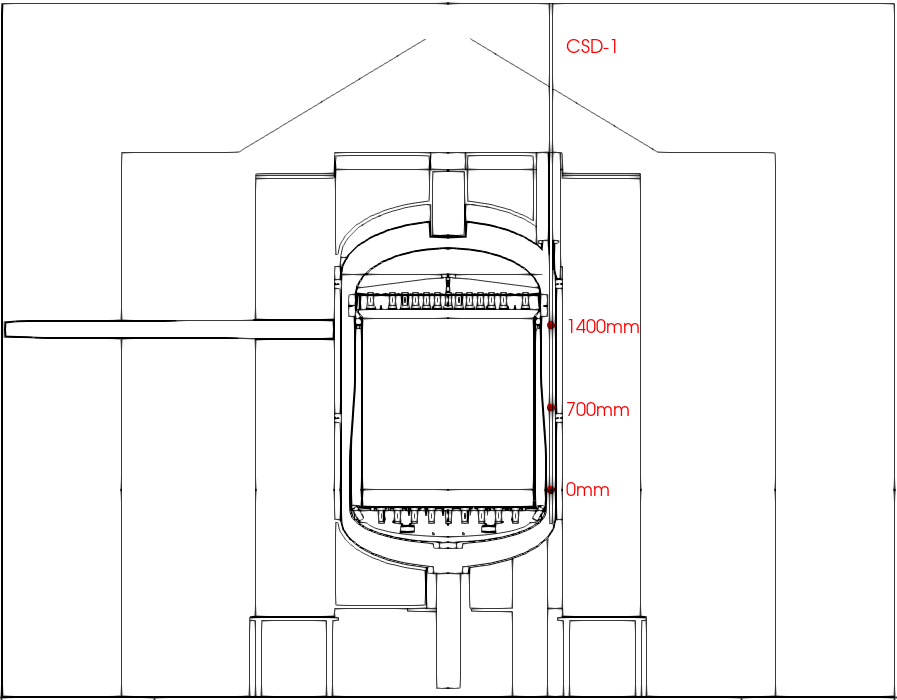
\includegraphics[width=\textwidth]{Figures/Geometry/csd1_geometry_black_and_white.png}
\caption{LZ geometry slice as implemented in GEANT4 from the water tank in. CSD-1 is shown along with the relevant Z-positions for calibration runs.}
\label{fig:CSD1_Geometry}
\end{figure}


\par
As the neutrons now originate outside of the TPC the \textbf{SS} had to be implemented.
The \textbf{SS} was defined as a cluster of activity close enough together that it cannot be distinguished and can be defined in energy deposit simulations as the energy-weighted variance in position being less than the detector spatial resolution.
This was determined from the result from LUX \cite{lux_position_reconstruction_ref}, scaled to LZ as per \cite{LZ_TechnicalDesignReview_ref} to give; ${\sigma}_{z}<0.2$ cm and ${\sigma}_{r}<3.0$ cm.
The \textbf{FID} is handled as before.
The result of the simulations are shown in \autoref{fig:simulated_amli_neutron_efficiency}.
\input{Chapters/OuterDetector/Figures/amli_efficiency_all_positions}

\par
The efficiency for an AmLi source at 0 mm is the first time the 95\% veto efficiency requirement is not met, yet it met for 1400 mm despite appearing to be in geometrically similar locations.
The difference can be account for in the reduced volume of the BATs compared to TATs + YBe plug, with area below the OCV being occupied by steel legs, water and foam.

\par
Perhaps unexpectedly, the veto efficiency varies depending upon the height of the source.
Part of the reason for this is shown in \autoref{fig:simulated_amli_capture_time} where the time it takes for the neutron to capture in the GdLS is shown.
Materials with a high $H$ content, such the foam and acrylic, can effectively moderate and bound the neutron in that material, restricting the neutrons ability to reach the OD.
The effect of this per volume can be seen in \autoref{fig:gdls_capture_time_vs_volume}, where the neutron capture time in the GdLS is plotted as a fraction of time the neutron spends in various materials.
In the capture constant this reflects itself as 2 exponential; one for a neutron that rapidly enters the GdLS and is moderated and captured there, and one for when the neutron is bouncing in a high-$H$ material before entering the GdLS.
In the latter case, the capture time constant is close to 200$\mu$s, corresponding to high-$H$ materials.
\par
The both the pure-LS and GdLS neutron capture times are well measured, with the most applicable for LZ from DayaBay, where the capture was modelled by \autoref{eq:neutron_capture_time} (Equation 15 in \cite{Dayabay_neutron_capture_fit_ref});
\begin{equation}
    N_{Gd}(t) = N_{0,Gd} \times [(1+\alpha)\frac{1}{\tau_{Gd}}e^{\frac{-1}{\tau_{Gd}}} - \alpha\frac{1}{\tau_{0}}e^{\frac{-t}{\tau_{0}}}] + C_{1} \\
\label{eq:neutron_capture_time}
\end{equation}
where the Gadolinium capture can be constrained by two time constants $\tau_{Gd}$, which represents the capture of thermal neutrons and $\tau_{0}$ for neutrons captured before thermalisation\footnote{This is actually neutrons from inverse $\beta$-decay with energies $\mathcal{O}$(0.015)MeV being captured before scattering enough to thermalise.}. 
$\alpha$ is simply a there to balance to two terms.
Given the much smaller volume of GdLS and the materials around it, there are most likely three exponents which contribute significantly to the capture time originating from; neutrons which enter the GdLS rapidly and thermalise and capture there, neutrons which scatter a lot in the foam before entering the GdLS, and neutrons which scatter in the acrylic multiple times before entering the GdLS.
The various neutron capture times for these mediums are shown in \autoref{tab:medium_neutron_capture_time}.
\begin{table}
\centering
\begin{tabular}{c|c}
    Medium  & Neutron Capture Time ($\mu$s)  \\ \hline
    GdLS    & 28 \cite{ucsb_gdls_dicebox_simulations_ref}  \\
    Water   & 202 \cite{snoplus_neutron_capture_time_on_water_ref}  \\
    Foam    & XX   \\
    Acrylic & XX  
\end{tabular}
\caption{Neutron capture time in pure and infinite mediums.}
\label{tab:medium_neutron_capture_time}
\end{table}
Given that the neutrons are being captured in the GdLS, the measured capture time from all mediums (except GdLS) will be lower than in \autoref{tab:medium_neutron_capture_time}. 
GdLS will be greater as the neutron not in infinite GdLS, but must travel through mediums less able to capture neutrons and so the effective capture time the neutron experiences will differ.

\input{Chapters/OuterDetector/Figures/amli_neutron_capture_time}

\input{Chapters/OuterDetector/Figures/gdls_capture_time_vs_volume}

\par
In practice any energy deposit will have to result in optical photons which are subject to the light collection efficiency (shown in \autoref{fig:od_lce}) for a photon to reach a PMT and the efficiency of the PMT to generate a signal (shown in \autoref{fig:od_pmt_qe}).
In order to determine the effect of this, full-propagation simulations were performed for a single AmLi calibration position, the 700 mm level.
This position was chosen as the energy deposit efficiency was closest to that of a 1 MeV neutron.

\par
As these simulations resulted in a detector signal, the full suite of LZ analysis tools were used, where the waveforms output from the simulated PMTs are run through a pulse finding algorithm and interaction finder, to identify single scatters.
The TPC contents of the event are reconstructed within the analysis package, providing both energy and position information of the event making the application of the analysis cuts is straight forward \cite{lz_simulations_ref}.
The OD veto energy threshold values were converted from energy to signal size using the values from a previous mock data challenge which are detailed in \cite{jonathannikoleyczik_thesis_ref}.
Additionally a PMT multiplicity cut was included.
It was set such that 5 or more PMTs needed to have contributed to the waveform in order for the pulse to be considered real\footnote{real in terms of coming from what we are searching for rather than a detector component or otherwise.}.
This was implemented to account for PMT effects, such as after pulsing and dark counts \cite{jonathannikoleyczik_thesis_ref}.
However no actual PMT effects, such as after pulsing and dark counts, were included in this simulation.

\par
The result of This is shown in \autoref{fig:simulated_amli_full_propagation_efficiency} for AmLi at 700mm. 
The neutron efficiency in this case never reaches the performance requirement at any energy threshold; reducing to 91\% for a 200 keV threshold with a 500 $\mu$s window window.
This is then the performance which can be expected during the calibration campaign (described later).

\input{Chapters/OuterDetector/Figures/amli_efficiency_700mm_full_propagation}

%\chapter{Analysis of the Outer Detector} \label{chap:analysis_of_the_od}

In this section analysis on the OD data during SR1 calibration and SR1 backgrounds is performed, with the goal of aces sing if the requirements set out in Table \ref{tab:veto_requirements} are met.

Rock gammas: https://arxiv.org/pdf/1706.00100.pdf

%\section{Discrimination Methods}

\par
There are countless different methods to discriminate different particles


\par
An important point to note is that the ability of any method to discriminate different event types is how the input variables are selected.
Ideally, each of the input variables would not be correlated with each other.
This is not the case, particularly as we have limited ourselves to using reduced quantities rather than raw waveforms.
So rather than doing pulse-shape discrimination, we are looking at some pre-extracted quantities of a given pulse.

\subsection{Maximum Likelihood Method}
\par
In shorterned form. 
For a given event, the likelihood for being of signal type is obtained by multiplying the signal probability densities of all input variables which are assumed to be independent and normalising this by the sum of the signal and background likelihoods.
Because correlations among the variables are ignored, this PDE approach is also called "naive Bayes estimator" \cite{TMVA_ref}.

Following the style of \cite{TMVA_ref}, the likelihood ratio $y_{\Lagrangian}$ of any event is defined as;
\begin{equation}
    y_{\Lagrangian} = \frac{\Lagrangian_{S}}{\Lagrangian_{S} + \Lagrangian_{B}}
\end{equation}
where
\begin{equation}
    \Lagrangian_{S,(B)} = \prod_k p_{S,(B),k}(x_k)
\end{equation}
where $p_{S,(B),k}$ is the signal (background) PDF for the kth input variable $x_k$.

%\section{Likelihood Implementation}
\par
In Section XXX the interactions that can occur are explained.
In SR1, the outer-detector is as a 'dumb' veto - this means that if any pulse in the OD that is within a given time frame of a Single Scatter in the TPC and is larger in pulseArea and PMT multiplicity that a loose value, then the entire event is vetoed.
As demonstrated during the TDR studies, this approach should be sufficient to achieve in excess a 95\% neutron rejection efficiency \cite{LZ_TechnicalDesignReview_ref}.

\par
This simple approach generally works well, but it does not maximise the OD.
For example, if it were possible to determine the type of or source of an interaction, then the uncertainty on backgrounds could be reduced.
Additionally, if an event is above the threshold for vetoing but is demonstrating that it is not from a WIMP-like particle, then the event would not have to be vetoed.
Together any PLR study, described in Section XXX, would be notably improved.

\subsection{How different sources look}
\par
A set of simulations were performed using the full-chain simulation chain described in Section XXX.
The output of this was analysed with LZap to produce a set of RQs.
The versions of reach software are shown in Table XXX.

\begin{table}[!htbp]
    \centering
    \begin{tabular}{c|c}
        Software & Version \\ \hline
        BACCARAT & XXX\\
        DER & XXX\\
        LZap & XXX
    \end{tabular}
    \caption{TODO...}
    \label{tab:od_simulation_versions}
\end{table}


\par
List potential RQs and where they come from (if they aren't been discussed before in the thesis)...
Then have a section on each of these variables to explain what it actually is.
Will have to go into information about pulse identification here then.
\subsubsection{pulseArea}
The pulse area is one of the most crucial variables used.
The number of photons detected is directly proportional to the energy of the interaction that occured.
Something about pulse selection...?

\subsubsection{coincidence}
More commonly referred to as pulse multiplicity, the coincidence value of a pulse is the number of PMTs which produced a signal that contributed to the pulse.
Generally this properly scales with the pulse Area, as the more photons produced by an interaction, the more will be detected, and so the more likely is it that any given PMT will see this light.
Given this, it can be questioned why this variable is used in addition to the pulse area. 
There are two reasons;
The first is that the variable must be used anyway for pulse selection in order to exclude after-pulsing.
The second is that it is a very robust and simple variable, and therefore ideal for early data as it is an easily understood quantity.

\subsubsection{Area Fraction Time over pulse area}
This variable is the most complicated of the selection.
The area fraction time, is the time (from the pulse start) to reach 75\% of the pulse integral.
It is essentially a measure of a limited pulse-width.
It has useful characteristics that make discrimination possible such as those shown in Fig XXX.
However, the quantity can be improved by combining it with a second variable; the pulse area.
This has the advantage of removing the pulse area as an influencing parameter in the value and making the variable more stable.
In the simplest case, the quantity gives is how fast or slow the pulse decreases after the peak.
An example of different interactions with this variable can be found in Figure XXX.

\subsection{Signal}

\subsection{Background}


%\section{Simulation Performance}

%\section{Calibration Performance}

\section{Backgrounds}
\label{sec:od_analysis_backgrounds}
\par
Using the aforementioned energy scale, noise cut, and scaling factor, in this section the background rate in the OD is measured and attempts are made to understand what is seen.
\par
In \autoref{fig:od_random_trigger} a comparison between the observed events in the OD during the entirety of SR1 and those expected are shown from the Random Trigger.
The expected rates are those described in \autoref{sec:simulated_od_requirements} and were simulated using the ``full-propagation" chain with the result scaled by the factor determined in the previous section.
Both data and simulations were handled by the same analysis tools, with the noise cut applied to both.
Included as well in \autoref{fig:od_random_trigger} is the expected rate in the OD if the GdLS had not undergo an improve purification.
Neither case fits what is observed particularly well.
More worryingly there is a peak in the data at 100 phd which does is not in the expected rate.


\input{Chapters/Analysis_OuterDetector/Figures/background_rates/od_random_trigger}

\par
In the remainder of this section, an attempt is made to understand what is observed and why it is different to what is expected.

\subsection{Rate Stability}

\par
To begin in the journey of understanding what is in the data, the first thing that was done was observe if the rate and distribution were stable over time.
Events from a month before the beginning of SR1 until the end were monitored every week using the Random Trigger.
The rate of events above the noise-cut, 100 keV and 200 keV were measured and are shown in \autoref{fig:OD_SR1_Rate}.
The noise-cut was applied as a base-cut, so the 100 keV is made up of the the noise-cut plus a phd cut, and similarly for 200 keV.
The three gaps in the data are when a calibrations were being performed.
This occurred three times in the region shown: just before SR1, 4 weeks into SR1, and straight after SR1.
\par
There are minor fluctuations in the noise-cut rate, but these are linked a xenon chiller and is consistent with a grounding failure, thus the behaviour is not mirrored in the 100 keV or 200 keV rates.
Importantly, over this period the OD rate remains stable, with no features in the observed distribution changing during that time.
Therefore what was shown in \autoref{fig:od_random_trigger} is the truly representative of the backgrounds in the OD.

\input{Chapters/Analysis_OuterDetector/Figures/background_rates/od_sr1_background_rate}

\par
Viewing the rate in a slightly different way, the rate-per-phd for the SR1 period is shown in \autoref{fig:od_sr1_rate_vs_threshold}.
Overlaid is the expected rate of backgrounds from \autoref{tab:od_expected_rates} for 100 and 200 keV.
Interestingly the rate above 100 keV is in fairly good agreement with what was predicted in \autoref{sec:simulated_od_backgrounds}.
This is consistent with being able to set the veto energy threshold to 100 keV, assuming that achieves an appropriate veto efficiency.
However differences arise at the 200 keV level, where the expected is 62.7$\pm$5.3 Hz were as the observed is 42.5$\pm$2.1 Hz, a fairly significant difference.

\input{Chapters/Analysis_OuterDetector/Figures/background_rates/od_rate_vs_threshold}

%%%%%%%%%%%%
\subsection{Position Reconstruction}
\par
Next we can look at the spacial distribution of events.
For any pulse it is possible to reconstruct the location of the interaction that caused the pulse by a weighted average such as:
\begin{equation}
    x = \frac{\sum{\text{Ch}_{\text{phd}} * \text{Ch}_\text{x}}}{\sum{\text{Ch}_\text{phd}}} 
\label{eq:OD_xy_position}
\end{equation}
where Ch$_{phd}$ is the phd of a PMT channel and Ch$_{x}$ is the position of the PMT.
Due to scheduling constraints associated with SR1, there was an insufficient variety of calibration sources were used at varying \{$x,y,z$\} positions in order to adequately determine the resolution of this approach, but it is something a future calibration campaign may be able to tackle. 
Additionally, this approach does not take into account the OCV in the centre of the detector, so reconstructed pulses will have an incorrect position, but the correct shape.
The OCV can be taken into account by converting coordinate system, but has explicitly not been done here due to the lack of knowledge in the actual resolution of this approach.
Regardless however, this approach does provide an insight in a way not thought possible based upon optical simulations.

\par
This approach was performed on slices in phd-space, the result of which can be seen in \autoref{fig:od_backgrounds_position_reconstruction}.
The first region focuses on the peak at 100 phd ($\backsim$ 0.5 MeV).
The second region focuses on the area above 2 MeV, where cavern-$\gamma$s should dominate.

\input{Chapters/Analysis_OuterDetector/Figures/background_constraints/od_background_positions}

\par
There are two useful observations in both regions.
Firstly, in $r-z$ there is a clear bias to events at the bottom of the detector.
This is consistent with cavern-$\gamma$s distribution shown in \autoref{fig:cavern_gamma_position_distribution}.
This indication that the cavern-$\gamma$s is the most significant contributor, again in agreement in the prediction (\autoref{tab:od_expected_rates}).
Secondly, in $x-y$ there is an elevated rate of events in \{$+x,+y$\}.
This can be understood easiest by labelling the SATs with letters A-D starting from \{$+x,+y$\} and going around clockwise.
Using this labelling, over the period of SR1, SAT A has a rate in excess of 8\% higher than any of the other tanks, with SAT B seeing the next highest rate (3\% higher than the mean).
Both SATs C and D saw an equivalent rate.
In \autoref{fig:OD_conduit_geometry}, the SAT placement are shown along with the conduits.
SAT A and SAT B are the only tanks which are obstructed by a single conduit, additionally both tanks cover an entire BAT and TAT.
The CSD-ports and the OCV legs block the other SATs from the TATs and BATs.
This results in the light having a more direct path to more PMTs and therefore higher probability of detection.

\begin{figure}[!htbp]
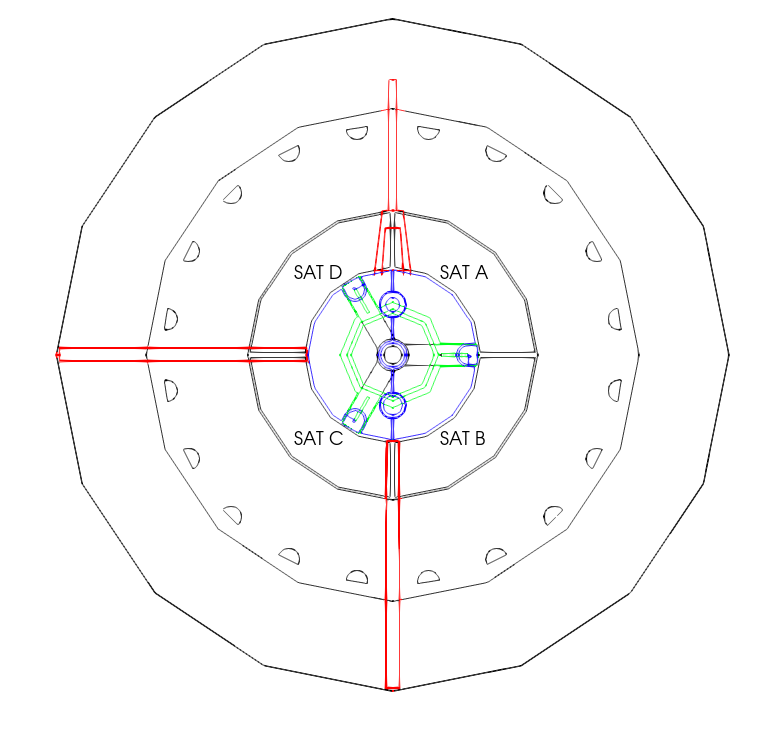
\includegraphics[width=\textwidth]{Figures/Geometry/geometry_with_conduits.png}
\centering
\caption{LZ geometry schematic. The OD geometry excluding the BATs and TATs is shown in black. The BATs and bottom on OCV are shown in green. The TATs, CSD ports and PMT conduits in blue. The DD calibration conduits and the High-Voltage feed through for the TPC are shown in red.}
\label{fig:OD_conduit_geometry}
\end{figure}


\par
As a way of suppressing cavern-$\gamma$'s is to take a slice in $z$, taking events reconstructed to be in the middle of the side tanks.
The resultant pulse area spectrum is shown in \autoref{fig:od_data_pulsearea_middle_tank}.
When compared to \autoref{fig:od_backgrounds_position_reconstruction} additional features appear around 300 phd.
These are consistent with ${}^{60}Co$ which is present in the OCV.
In future it may be possible to accurately measure the rate of this using this volume cut, but that will require a more dedicated calibration campaign, as the true quantity of the SAT selected is not clear.

\input{Chapters/Analysis_OuterDetector/Figures/background_constraints/od_middle_region_phd}


\subsection{$\gamma$ constraints}
\par
Another area to look at is high energy $\gamma$'s, from ($\alpha$,$\gamma$) reactions, which were discussed in \autoref{sec:cavern_gamma_generator}.
In \autoref{fig:od_high_energy} a the expected and observed rate per pulse area above 400 phd is shown.
The rate of events expected is significantly greater than that observed.
The findings here support the discussion in \autoref{sec:cavern_gamma_generator}, that the statistical model used does not extend well to ${}^{17}$O.
However, there are still features seen in data between 1000 and 1800 phd that are not accounted for in simulations.
These features have attributed to neutron captures on the Fe of the water tank (which is made of steel) producing high energy $\gamma$'s \autoref{iron_neutrons_ref}.
These neutrons originate primarily from the ${}^{252}$Cf calibration source, which was stored in a movable safe underground during SR1.
It was moved location within the cavern during SR1 which matches with a change in the reconstructed position of these events.
Backgrounds of this type were not previously considered within LZ, though are of great importance in fusion experiments \cite{iter_neutrons_ref}.
Primarily due to the source safe placement during SR1, it was not possible to determine if there was any fluctuation in the high-energy $\gamma$-rate during SR1.

\input{Chapters/Analysis_OuterDetector/Figures/background_constraints/od_high_energy}


%%%%%%%%%%%%
\subsection{$\alpha$ constraints}
\par
As was discussed in \autoref{sec:simulated_od_backgrounds} the exact rate of backgrounds from GdLS internals components is not known.
Fortunately we are able to constrain the some of the components. 
The decays within the U and Th decay chains all have an isotope in them with a half-life shorter than the LZ event window, of 4.5 ms.
It will therefore be possible to observe two decays from the same decay chain, which will appear as a pulse-pair (a pulse from each decay).
There are 3 possible decays, one from decay chain ${}^{238}$U, ${}^{235}$U and ${}^{232}$Th.
These are summarised in \autoref{tab:od_constrainable_decays_in_data}.
In reality though, only ${}^{214}$Bi$ \to {}^{214}$Po and ${}^{219}$Rn $\to {}^{215}$Po can be searched for as the interactions from ${}^{212}$Bi $\to {}^{212}$Po are close enough together that they will be merged into one pulse.

\begin{table}[!htbp]
    \centering
    \begin{tabular}{c|c|c|c|c|c}
        \multirow{2}{*}{Decay Pair (chain)}                    & \multicolumn{2}{c|}{First Decay}   & \multicolumn{3}{c}{Second Decay}    \\ 
                                                               & Decay    & Energy (MeV) & Decay    & Energy (MeV) & half-life ($\mu$s) \\ \hline
        ${}^{214}$Bi $\to {}^{214}$Po (${}^{238}$U$_{m}$)          & $\beta$  & 3.27         & $\alpha$ & 7.83         & 160   \\ 
        ${}^{219}$Rn $\to {}^{215}$Po (${}^{235}$U$_{l}$)          & $\alpha$ & 6.95         & $\alpha$ & 7.53         & 1800  \\ 
        ${}^{212}$Bi $\to {}^{212}$Po (${}^{232}$Th$_{l}$)         & $\beta$  & 2.25         & $\alpha$ & 8.95         & 0.3
    \end{tabular}
    \caption{Th and U decay chain pairs with half-lives within the LZ event window of 4.5 ms. 
             Decay information from \cite{radon_chains_ref}.
             See \autoref{fig:decay_chains} for the complete Decay Chains.}
    \label{tab:od_constrainable_decays_in_data}
\end{table}

\par
The decay pairs were searched for by looking for pulses which were reconstructed in be in close proximity to each other.
As the GdLS is not circulated and the decays particles ($\beta$ and $\alpha$) have do not have a significant penetrating power, the site of the two interactions with be very close to each other.
This position requirement acts to reduce the impact of coincident signals in other areas of the OD being mistakenly identified as part of the pulse pair.
The data selection criteria used was simply requiring that the reconstructed $z$ and $\theta$ be within some range of each other: $z_{\text{diff}} < 100$ and $\theta_{\text{diff}} < 1.0$, where diff refers to the difference between pulses.
It was also limited to pulses passing the noise-cut, primarily the PMT multiplicity (coincidence) requirements so that enough PMTs saw light to make the reconstruction meaningful.
This cut is fairly loose to account for potential variable inefficiencies in the position reconstruction with $z$ and $\theta$ based on pulse size.
The resultant pulse-pairs are shown in \autoref{fig:od_all_pulse_pairs_2d}.
Only pulses above 200keV in visible energy are included in the 2D histograms as the features are easier to see.

\input{Chapters/Analysis_OuterDetector/Figures/background_constraints/od_bipo_pulses_2d}

\par
In \autoref{fig:od_bipo_pulses_2d} there is a distribution where both the first and second pulse have a signal size around 170 phd.
These correspond to the double $\alpha$-decay in the ${}^{235}U_{l}$ chain.
The first pulse is slightly smaller than the second, which follows the pattern expected given the $\alpha$ energies shown in \autoref{tab:od_constrainable_decays_in_data}.
The second pulse-pair (from ${}^{238}U_{m}$) has a $\alpha$-decay in the same energy region, $\backsim$170 phd.
The first decay is a $\beta$-decay with the resultant electron have a spectrum of energies up the the end point of 3.27 MeV ($\backsim$ 400 phd).
As such even though the second pulse will be within a small range, there is no clear feature in \autoref{fig:od_bipo_pulses_2d} as the first pulse will be a wide range of values.

\par
It is still possible to isolate ${}^{214}$Bi $\to {}^{214}$Po but taking advantage of the much shorter decay half-life of ${}^{214}$Po vs ${}^{215}$Po.
This was done on the same same data as before with using the same position requirement, except now the time difference between the two pulses is considered.
The of time separation of the pulses has to be less than 800 $\mu$s.
This was selected as it is 5 full half-lives, in which 97\% of all ${}^{214}$Po will have decayed, and is less than half the half-life of ${}^{215}$Po.
The result of this is shown in \autoref{fig:od_time_dependent_pulses_2d}.
Included for completeness as well in \autoref{fig:od_time_dependent_pulses_2d} is the opposite case.
A new distribution has appeared is a second pulse size means of 240 phd, corresponding to the $\alpha$-decay of ${}^{214}$Po.

\par
The distributions in \autoref{fig:od_time_dependent_pulses_2d} allow for the rates of both ${}^{214}$Bi $\to {}^{214}$Po and ${}^{219}$Rn $\to {}^{215}$Po to be constrained.
This gives a rate of 98$\pm$2.5 mHz for ${}^{214}Bi \to {}^{214}Po$ and 7.7$\pm$1.2 mHz for ${}^{219}Rn \to {}^{215}Po$.
Both are rates are lower than those from expected from even the `improved purification' case (discussed in \autoref{sec:simulated_od_requirements}).


\par
Importantly, these constraints indicate that the $\alpha$-peak seen in \autoref{fig:od_random_trigger} is not from those subchains, as the rate would be too low.
This opens up the possibility that it is from ${}^{210}$Po from the late chain of ${}^{238}$U. 
This claim appears at odds with the relatively low internal rate of ${}^{238}$U.
However, it is known and measured that there is significant Rn in the cavern air, and as previously discussed (\autoref{sec:od_construction_sec}) the acrylic tanks were open to the air for long periods prior to installation.
There was opportunity for decay daughters to plate-out on the inside of the acrylic tanks, a feature that is of great concern within the TPC \cite{radon_plateout_ref}.
${}^{210}$Pb is the only long-lived particle in the Radon chain, with a half-life in excess of 22-years. 
The remainder of the isotopes would drastically reduce in abundance after a few weeks, leaving only ${}^{210}$Pb daughters visible, at a sustained rate.
This allows the acrylic holding the scintillator to act as a reservoir, providing a constant supply of $\alpha$ decays from ${}^{210}$Po.
LZ is not alone in having experienced this, with KamLAND measuring a higher than expected rate of ${}^{238}$U$_l$ decays \cite{KamLAND_LS_contaminants_ref}.

\par
The spectra for each of the three visible $\alpha$s are shown in \autoref{fig:od_extracted_alphas}.
The signal size has been converted into visible energy according by the energy scale previously discussed (\autoref{sec:od_energy_scale}).
Although it is unexpected to see a four $\alpha$'s, it becomes possible to perform an $\alpha$ energy calibration, and will be continuously measurable during all Science runs, without the need for Science data taking to be stopped.
An additional advantage is that PMT gain-drift will be more easily detectable.
The observed energy of each of the $\alpha$'s verse the observed energy are shown in \autoref{fig:od_alpha_quenching}, the Birk's law fit is also provided using the parameters in \autoref{tab:Birks_law_parameters}.
It can be seen that the parameters taken from pure LAB remain in good agreement with Gd-doped LAB used here.
This also isolates the difference between observed data and simulations to light propagation.

\input{Chapters/Analysis_OuterDetector/Figures/background_constraints/od_bipo_alphas}

\input{Chapters/Analysis_OuterDetector/Figures/background_constraints/alpha_quenching}


\subsection{${}^{152}$Gd}
\par
The final background that can be constrained is ${}^{152}$Gd, which produces a 2.2 MeV $\alpha$ decay ($\approx$ 120 keV visible energy).
The GdLS is loaded with 0.1\% (by mass) of natural Gadolinium.
With a total mass of GdLS used in the detector this corresponds to 16000kg, and ${}^{152}Gd$ has a natural abundance of 0.2\%, this gives a maximum possible rate of 27Hz, where there is a 5\% uncertainty on the doping by mass.
\par
Unfortunately this does not constrain does this region entirely.
Of particular note are ${}^{14}$C, a $\beta$ decay with an end-point of 156 keV, and ${}^{147}$Sm which decays via the emission of a 2.3 MeV $\alpha$.
All three were previously measured in the LS screener campaign, with ${}^{14}$C being the dominant contributor (>100 Hz) \cite{scotthaselschwardt_thesis_ref}.


\subsection{Background Fitting}
\par
Using all of the information of the OD backgrounds above, we finish this section is a fit of the expected background to the observed.
Simulations of all of the backgrounds identified in \autoref{sec:simulated_od_backgrounds}, but full light propagation and processed through the same analysis software suite as the observed data.
During this process the simulation signal sizes were scaled by 4.77.
Rather than fitting to the full observable space, a sub range was defined between 20 phd and 600 phd.
The lower limit was set so as to be far enough away from the noise-cut that any uncertainty in scaling factor would not remove these events.
The upper limit was set predominately by the rate of cavern-$\gamma$s.
In this region the expected background rate is 78.43$\pm$2.51 Hz.
This is slightly below the observed rate of 85.26$\pm$0.22 Hz.
\par
In order to keep the number of fit parameters down a number of steps were taken.
Firstly, all detector components were in combined. 
Secondly, contributions from ${}^{152}$Gd and ${}^{147}$Sm were combined together as the energy resolution is not sufficient to separate them.
The cavern-$\gamma$'s were allowed to float within the uncertainties they were measured in \cite{LZ_Gamma_Ray_Background_ref}.
${}^{238}$U$_l$ was allowed to fit between a range of [0, 15] Hz, where 15 is roughly double the size of the integrated rate of the peak at 100 phd above the background rest of the spectra.
${}^{238}$U$_{m}$ and ${}^{235}$U$_{l}$ were constrained by the rates previously reported.
All other backgrounds were left to allowed to float up to the maximum value measured in the LS screener campaign \cite{scotthaselschwardt_thesis_ref}.
\par
The result of the fit is shown in \autoref{fig:od_background_fit_to_data}.
Only components which contributed a more than 0.5 Hz to the OD rate have been included in \autoref{fig:od_background_fit_to_data}, but the fitted line should is from the all contributions.
The individual contributions of each component is shown in \autoref{tab:od_constrainable_decays_in_data}.

\par
${}^{238}$U$_l$ can successfully account for the peak observed at 100 phd, contributing in excess of 8 Hz to the OD rate.
The rate of cavern-$\gamma$s remain the background with the largest uncertainty for the backgrounds in the OD.
There remain some differences between the observed and fitted result, most notably at 50 phd where is a noticeable gap in a background that can fill in this region.
This can be incorporated as an uncertainty in the scaling factor.
The flat scaling of 4.77 did not take into account any position variation, and given that the light collection efficiency observed is significant greater than simulated, it is logical to suggest that the distribution in the LCE map (shown in \autoref{fig:od_lce}) is different as well.
This would effectively make contributions in lower light collection regions appear smaller than they are observed to be, which may go so way to explain what is seen.


\input{Chapters/Analysis_OuterDetector/Figures/background_fit/fit_result}


\begin{table}[!htbp]
    \centering
    \begin{tabular}{c|c|c}
        Source               &  Decay Type(s)               & Fitted Rate (Hz) \\ \hline
        \multicolumn{3}{l}{\textbf{Externals}} \\
        Cavern ${}^{238}$U   & $\gamma$                     & 7.65$\pm$1.65                    \\ 
        Cavern ${}^{232}$Th  & $\gamma$                     & 12.94$\pm$3.04                    \\ 
        Cavern ${}^{40}$K    & $\gamma$                     & 12.50$\pm$5.77                    \\ 
        Detector             & $\gamma$,$\beta$             & 3.63$\pm$0.67              \\ \hline
        \multicolumn{3}{l}{\textbf{Internals}} \\
        ${}^{238}$U$_{e}$     & $\gamma$,$\alpha$,$\beta$   & 0.98$\pm$0.21                    \\ 
        ${}^{238}$U$_{m}$     & $\gamma$,$\alpha$,$\beta$   & 0.03$\pm$0.10                   \\
        ${}^{238}$U$_{l}$     & $\gamma$,$\alpha$,$\beta$   & 8.74$\pm$2.34                \\
        ${}^{235}$U$_{e}$     & $\gamma$,$\alpha$,$\beta$   & 0.39$\pm$0.23                    \\
        ${}^{235}$U$_{l}$     & $\gamma$,$\alpha$,$\beta$   & 0.44$\pm$0.12                    \\
        ${}^{232}$Th$_{e}$    & $\gamma$,$\alpha$,$\beta$   & 0.18$\pm$0.04                    \\
        ${}^{232}$Th$_{l}$    & $\gamma$,$\alpha$,$\beta$   & 0.51$\pm$0.08                  \\
        ${}^{40}$K          & $\gamma$,$\beta$              & 0.05$\pm$0.01                 \\
        ${}^{14}$C          & $\beta$                       & 26.97$\pm$7.70           \\
        ${}^{176}$Lu        & $\gamma$,$\beta$              & 0.14$\pm$0.05               \\
        ${}^{147}$Sm and ${}^{152}$Gd    & $\alpha$         & 10.32$\pm$7.24                     
        
    \end{tabular}
    \caption{Fitting contributions of OD backgrounds to the observed data. The reported errors are statistical only.}
    \label{tab:od_constrainable_decays_in_data}
\end{table}

\subsection{Conclusion}
\par
To summarise this section, the OD rate for a number of months.
During this time the OD backgrounds were stable, with the rate above the noise-cut of 276.8 Hz, above 100 keV of 95.8 Hz and above 200 keV as 42.5 Hz.
The rate above 100 keV indicates that a veto time window of 500 $\mu$s is possible.
\par
Several background contributions have been measured in the OD and have been fitted against.
An un-expected contribution from ${}^{238}$U$_{l}$ is present which is believed to be from the radon emanation.
This entered all of the tanks via the frequent opening and closing the valves discussed in \autoref{sec:od_construction_sec}.


\section{Neutron Efficiency}
\par
For calculating the neutron efficiency during SR1 calibrations, AmLi was used.
As seen in \autoref{sec:sec:od_simulation_efficiency}, the efficiency is no longer expected to meet the requirement of 95\% efficiency.
But, as has been shown in the previous section, the simulation significantly underestimates the light collection efficiency, and so it's possible that the neutron propagation is also not modelled adequately.

\par
Three AmLi sources were used at the same time during this calibration, each placed in a different CSD tube.
This is summarised in \autoref{tab:amli_source_activities}.

\begin{table}[!htbp]
    \centering
    \begin{tabular}{c|c|c}
        CSD & AmLi Source No. & Activity (n/s) \\ \hline
        1   & Source-2        & 13.8           \\
        2   & Source-1        & 9.3            \\ 
        3   & Source-3        & 11.9                
    \end{tabular}
    \caption{AmLi source activities in each CSD}
    \label{tab:amli_source_activities}
\end{table}

\par
For this data, the S2-trigger was used, and the cuts developed for the WIMP search were used to filter out unusable data, to leave a fairly pure dataset of neutron recoils.
These are summarised below, but are detailed in \cite{lz_ws_sr1_ref};

\begin{enumerate}
    \item \textbf{SS}: Single Scatter cut as determined by the interaction finder, shown to be 98.5\% efficient.
    \item \textbf{S2Cuts}: Remove events where the S2 pulse has unusual properties.
    \item \textbf{S1Cuts}: Remove events where the S1 pulse has unusual properties.
    \item \textbf{FID}: Fiducial Volume, to remove wall events and ensure that the neutron penetrated deep enough.
    \item \textbf{NR}: Select events that have nuclear recoiled by selecting events within 1-$\sigma$ of the NR band, which was calibrated using the external DD neutron source.
\end{enumerate}

\par
Three positions in the CSD were used, 0mm, 700mm and 1400mm. 
These definitions are identical to those used in \autoref{sec:od_simulation_efficiency}.
The result of applying the selection cuts to these runs is shown in \autoref{tab:amli_calibration_summary}.

\begin{table}[!htbp]
    \centering
    \begin{tabular}{c|c|c|c|c}
        \multirow{2}{*}{z position (mm)} & \multirow{2}{*}{Run IDs}  & \multicolumn3{c}{Number}  \\ 
                                         &                           & Events    & SS & passing all cuts     \\ \hline
        0                                & 8350-8369                 & 5,504,700 & X  & X               \\
        700                              & 8304-8317                 & 3,688,200 & X  & X               \\ 
        1400                             & 8319-8348                 & 7,041,500 & X  & X                
    \end{tabular}
    \caption{Summary of AmLi source deployment during post SR1 calibrations}
    \label{tab:amli_calibration_summary}
\end{table}

\par
From these events it is then possible to search for events that occur after the S1 in both the Skin and OD.
Those events which pass the TPC cuts are shown in XXX.




\par
Using the maximum veto window for 200keV of 1200$\mu$s, the efficiency as a function of photons detected is shown in \autoref{fig:commissioning_amli_efficiency_per_phd}.
The combined veto efficiency of the Skin and OD are used here due to the limited impact the Skin has on the veto efficiency of neutrons.

\input{Chapters/Analysis_OuterDetector/Figures/efficiency/amli_efficiency_per_phd}


\par
Due to the poorer than expected performance of the OD for tagging neutrons, the decision was made to use the longer veto window of 1200$\mu$ combined with a 200keV pulse requirement in the OD or a 100keV requirement in the Skin.
The result of this is summarised in \autoref{fig:commissioning_amli_efficiency_with_bg_rate}.

\input{Chapters/Analysis_OuterDetector/Figures/efficiency/amli_final_efficiency}


\par
On SR1 WIMP-search data, this has a total impact of 4.99\% on live-time, and the resultant events which were vetoed are shown in Figure XXX.
No neutrons were vetoed in SR1 which corresponds to no neutrons being expected.
The events which were vetoed were electron recoil events which were coincidence with an OD background.

\begin{figure}[!htbp]
    \centering
    
\includegraphics[width=0.5\textwidth]{Figures/Placeholder.png}
    \caption{Effect on SR1 data before and after the \textbf{Veto} cut.}
    \label{fig:tpc_with_od_veto_in_sr1}
\end{figure}

\par
The AmLi 

\input{Chapters/Analysis_OuterDetector/Figures/efficiency/sr1_vetoed_events}


\subsection{Neutron Captures}
\par
Although AmLi 
Another source that can be used to study the neutron capture time is the ${}^{252}{Cf}$ calibration source.
Spontaneous fission of ${}^{252}{Cf}$ typically results in a number of $\gamma$'s with a combined energy of up to 10MeV which are accompanied by a number of neutrons.
An example event from the LZ calibration run pre-SR1 is shown in \autoref{fig:cf252_event_viewer}.
This allows for neutrons to be tagged by tagging the fission by coincident $\gamma$'s in a each detector, and assuming later pulses are dominated by neutrons.

\begin{figure}[!htbp]
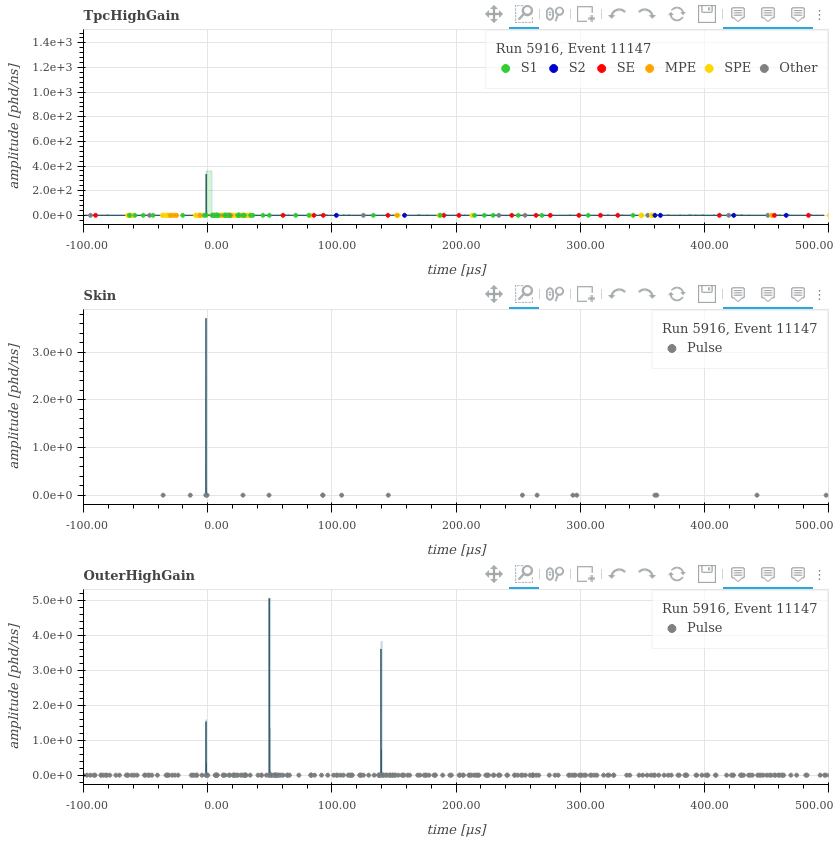
\includegraphics[width=\textwidth]{Figures/NeutronCaptureTime/cf252_eventviewer_5916.png}
\centering
\caption{Example event from ${}^{252}{Cf}$ calibration run showing the $\gamma$'s causing coincident pulses in each detector followed by two neutrons being captured in the Outer Detector}
\label{fig:cf252_event_viewer}
\end{figure}

\par
Although \autoref{fig:cf252_event_viewer} indicates that prompt $\gamma$'s can be used for tagging it does come with a significant caveat; namely that expressed in \autoref{fig:fission_fragments_time}.
There is a non-insignificant probability that $\gamma$'s will be emitted at the same time as a $\gamma$ from a neutron capture is released.
Additionally the majority of study into prompt $\gamma$'s from fission focus on the first 100ns post-fission and the energy and multiplicity beyond that time is not well theorised. 
However, by selecting events which only have a double or triple detector coincidence this can be mitigated.


\begin{figure}[!htbp]
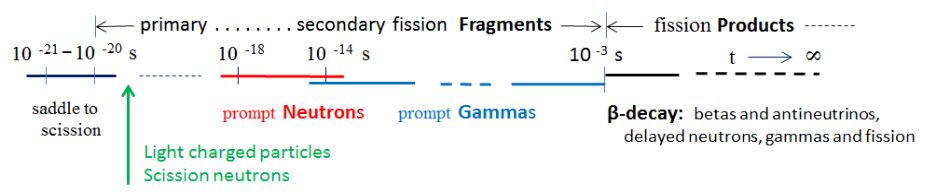
\includegraphics[width=13cm]{Figures/NeutronCaptureTime/fission_fragment_times.png}
\centering
\caption{Emission time-frame of fission components. Adapted from \cite{cf252_fission_ref}}
\label{fig:fission_fragments_time}
\end{figure}

\input{Chapters/Analysis_OuterDetector/Figures/neutron_capture/cf252_pulse_selection}

\input{Chapters/Analysis_OuterDetector/Figures/neutron_capture/cf252_largest_after_pulse}

\input{Chapters/Analysis_OuterDetector/Figures/neutron_capture/cf252_capture_time}

\par
The best fit was found to be with just two exponents.
With $t_0 = 31.39 \pm 0.4\mu s$ and $t_1 = 124.5 \pm 1.7\mu s$, with a $\chi^2=0.821$.
$t_0$ accounts for neutrons which travel straight through from the source position to the GdLS and are captured on the GdLS.
$t_1$ is more complex as it accounts for neutrons scatter several times in not the GdLS, such as the acrylic of foam regions.
Given each of these have a different affect on this, it is not clear exactly what is causing it.
This is particularly apparent when compared to the expected result from simulations (also included in \autoref{fig:cf252_gd_capture_time}, where we can see that the neutrons are taking longer than expected to be captured in the OD.
This indicates that neutrons are becoming trapped in materials between the calibration tube and the OD.
The possible materials between the CSD and the OD are primarily foam, acrylic and water.
Given that the acrylic thickness was measured during construction, this leaves water as the most likely scenario.

\par
One possible reason for this is the foam surrounding the OCV not stopping all water from coming into that region.
Though when the SATs were installed, there was no discernible gap between the SAT and the Tyvek around the OCV foam.
Though it is possible that a small amount of water would have entered this area over time, but no more than a few mm.

\par
Another possibility is that the foam became at least in part filled with water.
Water ingress in foam has been well studied at least in part, with the industrial measures of water absorption defined as via diffusion and by submersion \cite{foam_with_water_ref}.
The effectiveness of any foam type to keep water out is based on a number of factors including density and most importantly if the structure is closed or open\footnote{in terms of whether the cells which make up the foam structure. Open cell foams are softer and more flexible as each cell is open to the atmosphere. Closed cell foams are firmer with the majority of cells being closed to the atmosphere.}.
The difference in terms of water ingress is shown in \autoref{fig:foam_mri_water_ingress}.


\begin{figure}[!tbhp]
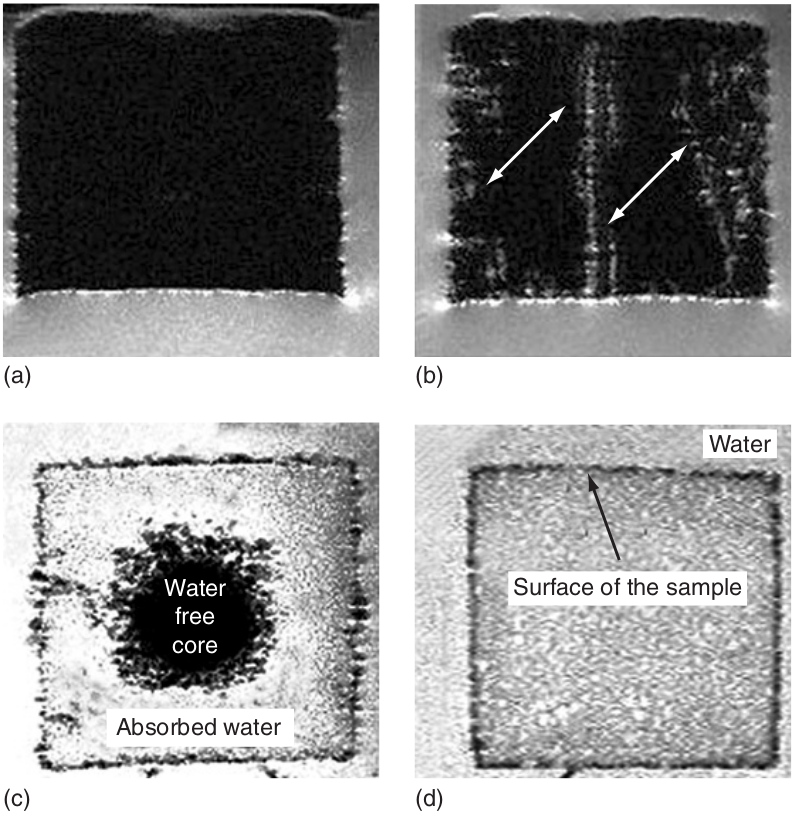
\includegraphics[width=\textwidth]{Figures/NeutronCaptureTime/foam_water_absorption.png}
\centering
\caption{Magnetic resonance images of 30 mm cube samples of polyurethane foam for two types of different foam of the same density, 0.3 g m${}^{-3}$: a closed cell foam (top) and an open cell foam (bottom).
(a) closed cell foam after 8 hours. (b) closed cell foam after 63 hours.
(c) open cell foam after 8 hours. (d) open cell foam after 72 hours.
Images from \cite{foam_mri_data_ref}.
}
\label{fig:foam_mri_water_ingress}
\end{figure}


\par
The foam installed around the OCV (green foam in \autoref{sec:od_construction_sec}) is a closed cell foam expanded using $CO_2$, so each cell is filled with $CO_2$, foam 3000 CS in \cite{styrodur_water_ingress_ref}.
As such the foam is expected to experience a 0.7\% volume ingress of water due to long term submersion and 5\% volume ingress of water from diffusion\footnote{long-term in this case refers to a 28-day test as is the industry standard, see BS EN ISO 16535 (previously BS EN 12087) and BS EN ISO 16536 (previously BS EN 12088).}.
These values, being based off of tests designed of industry do not necessarily map obviously onto how it was used in this application, particularly given that water pressure is not considered in the industrial tests and the long-term are orders of magnitude less than the exposure the LZ foam has had already.
\par
In order to begin probing this, a test was conducted to observe what happens to this foam (and what happens to the water).
An example of each piece of foam used, was placed in de-ionised water and placed under a $N_2$ purge. 
The water resistivity was measured every few hours as a monitor of the water's purity.
The result over the first week of running is shown in \autoref{fig:od_foam_degredation}.
What is observed during this period is the water becoming contaminated with ions from the foam from out gassing.
Over a longer period of study it may show that the foam becomes saturated with water, particularly with a test using a piece of foam shaped to the same dimensions as those used in the installation.
\par
The foam installed between the TATs and OCV are held together with HandiFoam\textsuperscript{\textregistered}, which also forms a closed cell structure: not only does the outer layer is enclosed everything, but the inner structure is 95\% closed cell.
However, due to it's low-pressure it is classified as "vapour retardant", and prolonged exposure to water will rapidly saturate the foam \cite{handifoam_water_ingress_ref}.
The speed at which this occurred was likely accelerated by the cutting into the outer layer, done to shape the foam to size.
\par
The other foam of concern is the polyethylene foam \cite{white_foam_ref}, which is also a closed-cell structure, though with a much finer cell structure.
Though as it's purpose was primarily padding, and the quantity installed is low, water displacement is of less concern.
Only around the BATs is a neutron able to reach the foam before reaching the GdLS.

\par
In relation to LZ, this has two impacts, firstly these ions can circulate throughout the OD water and contribute to the low energy rate.
Secondly, this will impact on the time it takes for a neutron to reach the GdLS.
Taking the most extreme case as the foam being completely replaced with water, we can see that the neutron time to reach the GdLS is significantly increased (shown in blue in \autoref{fig:data_vs_sim_gd_capture_time}).
This therefore seems an reasonable explanation for the difference observed, though some tuning is required for a closer match between the simulation and observed.


\input{Chapters/Analysis_OuterDetector/Figures/neutron_capture/foam_degredation}

\input{Chapters/Analysis_OuterDetector/Figures/neutron_capture/data_vs_sim_capture_time}


\section{Particle Discrimination}
\par
As previously mentioned, the OD has been designed to act as an "active but dumb" veto.
It could be improved by including some form of interaction identification in the OD.
For example, the Bi-Po interactions in Section XXX can be identified from two interactions in close proximity to each other with relative ease.
These events could then be un-vetoed; increasing the number of candidate events as well as the live-time.

\par
There is also the possibility of discriminating between high energy backgrounds such as neutron captures and cavern-$\gamma$'s.
This would actually be a discrimination between 1-$\gamma$ vs multiple $\gamma$'s.
The viability of this discrimination in simulated datasets is explored in this section.


\subsection{Maximum Likelihood Method}
\par
\par
An important point to note is that the ability of any method to discriminate different event types is how the input variables are selected.
Ideally, each of the input variables would not be correlated with each other.
This is not the case, particularly as we have limited ourselves to using reduced quantities rather than raw waveforms.
So rather than doing pulse-shape discrimination, we are looking at some pre-extracted quantities of a given pulse.

\par
In shorterned form. 
For a given event, the likelihood for being of signal type is obtained by multiplying the signal probability densities of all input variables which are assumed to be independent and normalising this by the sum of the signal and background likelihoods.
Because correlations among the variables are ignored, this PDE approach is also called "naive Bayes estimator" \cite{TMVA_ref}.

Following the style of \cite{TMVA_ref}, the likelihood ratio $y_{\Lagrangian}$ of any event is defined as;
\begin{equation}
    y_{\Lagrangian} = \frac{\Lagrangian_{S}}{\Lagrangian_{S} + \Lagrangian_{B}}
\end{equation}
where
\begin{equation}
    \Lagrangian_{S,(B)} = \prod_k p_{S,(B),k}(x_k)
\end{equation}
where $p_{S,(B),k}$ is the signal (background) PDF for the $k^{th}$ input variable $x_k$.


\subsection{Variables}
\par
A set of simulations were performed using full-chain propagation; particle propagation and PMT modelling.
The resultant waveforms were passed to the reconstruction package.
From the reconstruction, 3 variables were selected to describe a pulse.
The variables, which are described below, were chosen as they are relatively simple.
Meaning that there has been limited manipulation of the raw event data.
Figure XXX shows the variables against one another for a variety of sources.


\paragraph{coincidence}
Sometimes referred to as pulse multiplicity, the coincidence value of a pulse is the number of PMTs which produced a signal that contributed to the pulse.
As the more photons produced, the more will be detected, and so the more likely is it that any given PMT will see this light.
It is a very robust and simple variable, and therefore ideal to start with.
A neutron capture will likely have a higher coincidence as the multiple $\gamma$'s can scatter in different areas of the OD.


\paragraph{pulse area}
The number of photons detected is directly proportional to the energy of the interaction that occurred.
Combined with the coincidence, it has the potential to isolate unwanted pulses such as those caused by PMT after-pulsing.


\paragraph{$\frac{\text{width}}{\text{pulse area}}$}
This variable is the most complicated of the selection, which gives a pulse-shape.
The width of a pulse is the time.
Due to pulse finding limitations, the full reconstructed pulse width was not used.
Instead, the pulse start time was defined as; the time where 5\% of the pulse integral was reached, and the end time as 75\% of the pulse integral.

However, the quantity can be improved by combining it with a second variable; the pulse area.
This has the advantage of removing the pulse area as an influencing parameter in the value and making the variable more stable.
In the simplest case, the quantity gives is how fast or slow the pulse decreases after the peak.
An example of different interactions with this variable can be found in Figure XXX.

\begin{figure}[!htbp]
    \centering
    
\includegraphics[width=0.5\textwidth]{Figures/Placeholder.png}
    \caption{Variables used for particle discrimination}
    \label{fig:discrimination_variables}
\end{figure}

\input{Chapters/Analysis_OuterDetector/Figures/likelihood_variables}

\subsection{Performance}
\par
For this study, the signal was selected to be neutron captures and the background as cavern-$\gamma$'s
The neutron captures were simulated by starting thermalised neutrons in the GdLS.
This meant that only the energy deposits in the OD as a result post-capture were detectable.
The 
\par
The likelihood was performed against a set of simulations which contained a mixture of both neutron captures and cavern-$\gamma$'s in quantities expected \cite{LZ_assay_ref}.
The neutrons were, as above, thermalised so the only interaction of note are from the result of neutron captures.






\begin{figure}[!htbp]
    \centering
    
\includegraphics[width=0.5\textwidth]{Figures/Placeholder.png}
    \caption{ROC curve of}
    \label{fig:discrimination_performance}
\end{figure}

\par
Although it is possible to use this method with data, it has been impractical given the differences mentioned earlier in this Chapter.
In order to perform this, a data-driven approach is required and simulation corrections implemented.
Both of which have not been performed due to time constraints.





\par
Interaction discrimination based upon a likelihood has the potential to improve the OD effectiveness; reducing the dead-time as as result of false vetoes.
It can also reduce the uncertainties on backgrounds - particularly if combined with detector coincidences on Gd-captures as was done in Section XXX.
There is scope for additional interesting studies such as seasonal modulation in rates of interactions such as ($\alpha$,$\gamma$) \cite{cavern_gammas_in_Soudan_mine_ref}.
All of these together can directly improve the sensitivity of LZ to a potential dark matter detection.

\par
Once data is better understood, it may be possible to implement higher dimensional variables to discriminate interactions.
Though all of these are subject to an eventual match-up in simulation and data.


%\chapter{Analysis of Effective Field Theory Interactions in LZ}
\label{chap:eft_work}
In this final analysis chapter we pull together many of the concepts touched on in this Thesis to perform a dark matter search, and ultimately setting limits on the each of the 
We use our model independent approach from \autoref{chap:detection_theory} along with the PLR in CHAPTER XXX

\par
To re-emphasise what was said in CHAPTER XXX, in order to perform any each for a rare events (in our case nuclear recoils) you need to understand the discrimination between ER and NR events, and you need a detailed understanding of backgrounds.




%\begin{figure}[!htbp]%
\centering
\begin{tikzpicture}
\centering
  \begin{groupplot}[view={0}{90},
    group style = {group size = 2 by 4,
                   vertical sep=1.5cm,
                   horizontal sep=2.0cm}]
    
    \pgfplotsforeachungrouped \x in {1,3,4,5,6,7,8,9}{
     \edef\tmp{
        \noexpand \nextgroupplot[
                                xlabel=Mass (MeV),
                                ylabel=$({c}^{s}_{\x}\times{m}^{2}_{w})^{2}$,
                                mark size=0pt,
                                width=0.45\textwidth,
                                height=5.5cm,
                                xmode=log,
                                ymode=log,
                                x label style={at={(axis description cs:0.75,-0.1)},anchor=near ticklabel},
                                y label style={at={(axis description cs:-0.13,.75)},anchor=near ticklabel},
                                ]
            
            \noexpand \addplot[blue, name path = xenon100] table[]
                      {Data/HENR/Xenon100/O\x.dat};
                        
            \noexpand \addplot[only marks, mark size=1, error bars/.cd,
                               y dir=both, y explicit, error bar style={color=black}]
                               table[x=mass,y=median, y error plus index=3, y error minus index=2] {Data/HENR/Projected_Sensitivity/LUX/O\x.dat};
            
            \noexpand \addplot[green, opacity = 0.4, name path = nsig1] table[x=mass, y=nsig1]
                      {Data/HENR/Projected_Sensitivity/Results_method1/O\x.dat};
                      
            \noexpand \addplot[green, opacity = 0.4, name path = psig1] table[x=mass, y=psig1]
                      {Data/HENR/Projected_Sensitivity/Results_method1/O\x.dat};
                      
            \noexpand \addplot[yellow, opacity = 0.4, name path = psig2] table[x=mass, y=psig2]
                      {Data/HENR/Projected_Sensitivity/Results_method1/O\x.dat};
                      
            \noexpand \addplot[green, opacity = 0.4, forget plot] fill between[of=nsig1 and psig1];
            \noexpand \addplot[yellow, opacity = 0.4, forget plot] fill between[of=psig1 and psig2];
            
            \noexpand \addplot[black, name path = median] table[x=mass, y=median]
                      {Data/HENR/Projected_Sensitivity/Results_method1/O\x.dat};
            
            %\noexpand \addplot[black, dashed, name path = median] table[x=mass, y=cl]
            %          {Data/HENR/Projected_Sensitivity/Results/O\x.dat};
                     
        }
        \tmp 
        }
  \end{groupplot}
\end{tikzpicture}
\caption{}
\label{fig:EFT_Result_Projected_Sensitivity_1}
\end{figure}



\begin{figure}[!htbp]%
\centering
\begin{tikzpicture}
\centering
  \begin{groupplot}[view={0}{90},
    group style = {group size = 2 by 3,
                   vertical sep=1.5cm,
                   horizontal sep=2.0cm}]
    
    \pgfplotsforeachungrouped \x in {10,11,12,13,14,15}{
     \edef\tmp{
        \noexpand \nextgroupplot[
                                xlabel=Mass (MeV),
                                ylabel=$({c}^{s}_{\x}\times{m}^{2}_{w})^{2}$,
                                mark size=0pt,
                                width=0.45\textwidth,
                                height=5.5cm,
                                xmode=log,
                                ymode=log,
                                x label style={at={(axis description cs:0.75,-0.1)},anchor=near ticklabel},
                                y label style={at={(axis description cs:-0.13,.75)},anchor=near ticklabel},
                                ]
            
            \noexpand \addplot[blue, name path = xenon100] table[]
                      {Data/HENR/Xenon100/O\x.dat};
            
            \noexpand \addplot[only marks, mark size=1, error bars/.cd,
                               y dir=both, y explicit, error bar style={color=black}]
                               table[x=mass,y=median, y error plus index=3, y error minus index=2] {Data/HENR/Projected_Sensitivity/LUX/O\x.dat};
                        
            \noexpand \addplot[green, opacity = 0.4, name path = nsig1] table[x=mass, y=nsig1]
                      {Data/HENR/Projected_Sensitivity/Results_method1/O\x.dat};
                      
            \noexpand \addplot[green, opacity = 0.4, name path = psig1] table[x=mass, y=psig1]
                      {Data/HENR/Projected_Sensitivity/Results_method1/O\x.dat};
                      
            \noexpand \addplot[yellow, opacity = 0.4, name path = psig2] table[x=mass, y=psig2]
                      {Data/HENR/Projected_Sensitivity/Results_method1/O\x.dat};
                      
            \noexpand \addplot[green, opacity = 0.4, forget plot] fill between[of=nsig1 and psig1];
            \noexpand \addplot[yellow, opacity = 0.4, forget plot] fill between[of=psig1 and psig2];
            
            \noexpand \addplot[black, name path = median] table[x=mass, y=median]
                      {Data/HENR/Projected_Sensitivity/Results_method1/O\x.dat};
            
            %\noexpand \addplot[black, dashed, name path = median] table[x=mass, y=cl]
            %          {Data/HENR/Projected_Sensitivity/Results/O\x.dat};
                     
        }
        \tmp 
        }
  \end{groupplot}
\end{tikzpicture}
\caption{}
\label{fig:EFT_Result_Projected_Sensitivity}
\end{figure}

%\section{Signal Model}
\par
The actual signal model is actually produced by taking a theoretical event rate spectrum (produced by a Mathematica package - DMFormFactor - developed by XXX) and applying the analysis acceptance and detector response.
Passing through LZLama or PdfMaker, this turns the above into event observable - S1 and LogS2).
\par
DMFormFactor takes performs the calculations described previously.
Each Xenon isotope is evaluated separately and is weighted by the Xenon abundance before being added together to produce an energy spectrum.
As mentioned previously, the energy spectrum is dependant upon the choice of coupling and the WIMP mass.
\par
The choice has been made to perform analysis in iso-scalar rather than proton-neutron. 
There is always an argument that one approach is more appropriate than the other
\par
In table \ref{tab:DMFormFactor_parameters} the parameters used for this are shown.
The majority of these values are to match those from previous studies and the Dark Matter community standards.

\begin{table}[]
    \centering
    \begin{tabular}{c|c}
        Parameter   & Value  \\ \hline
        $\nu_0$     & 220$km s^{-1}$ \\
        $\nu_{esc}$ & 544$km s^{-1}$ \\
        $\rho_{0}$     & 0.3 $GeV/cm^{3}$ \\
        $\nu_E$     & 245 $km s^{-1}$ 
    \end{tabular}
    \caption{DMFormFactor parameters used for the standard halo model. CITE XXX}
    \label{tab:DMFormFactor_parameters}
\end{table}


\par
A subset of the recoil spectra calculated are shown in Figures \ref{fig:HENR_Spin_Recoil_Spectrum} and \ref{fig:HENR_NotSpin_Recoil_Spectrum}.
The masses for which the energy spectra were calculated were;
[5, 7, 10, 12, 14, 21, 33, 50, 100, 200, 400, 1000, 4000] GeV all of which can be seen in Annex XXX.
The reason for this is that the shape of the limit produced is fairly well understood, so only a subset of WIMP masses are needed.

\newcommand{\allrecoiloperators}{01s,03s,04s,05s,06s,07s,08s,09s,10s,11s,12s,13s,14s,15s}
\newcommand{\spinrecoiloperators}{01s,04s,06s,07s,09s,10s,11s,14s}
\newcommand{\roguerecoiloperators}{03s,05s,08s,12s,13s,15s}

\begin{figure}[!htbp]%
\centering
\begin{tikzpicture}
\centering
  \begin{groupplot}[view={0}{90},
    group style = {group size = 2 by 1}]
    \nextgroupplot[
    xlabel=Recoil Energy (keV),
    ylabel=Differential Rate (kg/day/keV),
    legend pos=north east,
    mark size=0pt,
    xmin=1, xmax=400, xmode=log,
    ymin=1e-14, ymax=1e3, ymode=log]
    \foreach \henrop in \spinrecoiloperators{
                \addplot 
                    table
                    %{Data/HENR/Signal/Recoils/dRdEr_EFT_O01s_m5GeV_0.txt};
                    {Data/HENR/Signal/Recoils/dRdEr_EFT_O\henrop_m5GeV_0.dat};
            }
    \nextgroupplot[
    xlabel=Recoil Energy (keV),
    legend pos=north east,
    mark size=0pt,
    xmin=1, xmax=400, xmode=log,
    ymin=1e-14, ymax=1e3, ymode=log]
    \foreach \henrop in \spinrecoiloperators{
                \addplot
                    table
                    %{Data/HENR/Signal/Recoils/dRdEr_EFT_O01s_m5GeV_0.txt};
                    {Data/HENR/Signal/Recoils/dRdEr_EFT_O\henrop_m21GeV_0.dat};
            }
  \end{groupplot}
\end{tikzpicture}
\caption{Literal Aids
\textbf{Left:} $Gd^{156}$ de-excitation path.
\textbf{Right:} $Gd^{158}$ de-excitation path.
}
\label{fig:HENR_Spin_Recoil_Spectrum}
\end{figure}

\begin{figure}[!htbp]%
\centering
\begin{tikzpicture}
\centering
  \begin{groupplot}[view={0}{90},
    group style = {group size = 2 by 1}]
    \nextgroupplot[
    xlabel=Recoil Energy (keV),
    ylabel=Differential Rate (kg/day/keV),
    legend pos=north east,
    mark size=0pt,
    xmin=1, xmax=400, xmode=log,
    ymin=1e-14, ymax=1e3, ymode=log]
    \foreach \henrop in \roguerecoiloperators{
                \addplot 
                    table
                    %{Data/HENR/Signal/Recoils/dRdEr_EFT_O01s_m5GeV_0.txt};
                    {Data/HENR/Signal/Recoils/dRdEr_EFT_O\henrop_m5GeV_0.dat};
            }
    \nextgroupplot[
    xlabel=Recoil Energy (keV),
    legend pos=north east,
    mark size=0pt,
    xmin=1, xmax=400, xmode=log,
    ymin=1e-14, ymax=1e3, ymode=log]
    \foreach \henrop in \roguerecoiloperators{
                \addplot
                    table
                    %{Data/HENR/Signal/Recoils/dRdEr_EFT_O01s_m5GeV_0.txt};
                    {Data/HENR/Signal/Recoils/dRdEr_EFT_O\henrop_m5GeV_0.dat};
            }
  \end{groupplot}
\end{tikzpicture}
\caption{Literal Aids
\textbf{Left:} $Gd^{156}$ de-excitation path.
\textbf{Right:} $Gd^{158}$ de-excitation path.
}
\label{fig:HENR_NotSpin_Recoil_Spectrum}
\end{figure}

\par
When performing this analysis, an important choice is the coupling choice.


\paragraph{Copied from Billy}
\par
To allow for ease of comparison to previous limit setting on the inelastic36
WIMP-nucleon EFT operators by the XENON collaboration [? ], this analysis was conducted in the isoscalar basis.37
In the isoscalar basis, the charge densities of the nucleons are effectively averaged such that the interaction becomes38
indiscriminate to the type of nucleon involved, even though both the isoscalar and proton-neutron basis provide insight.39
For this WIMP-nucleon EFT, the UV scale governing the physics is far higher than the energies that are probed in the40
experiment. At these lower energies, the UV interactions have to be reduced to effective ones, which is done at the u,41
d and s quark level. The assumption is made that the couplings to each quark at these scales are roughly equivalent.42
Therefore the mass differences of these quarks are negligible at the high-energy scale of the underlying physics, and the43
interaction would be isoscalar. By performing this analysis in the isoscalar basis, it is possible to test this assumption’s44
validity. Additionally, by using either an isoscalar or isovector basis, the target’s nuclear state can be considered as45
isospin symmetric; a property of the strong force that can aid in simplifying the analysis.

\begin{figure}
    \centering
    
\includegraphics[width=0.5\textwidth]{Figures/Placeholder.png}
    \caption{Integrated rate for each operator for a 1000GeV DM particle}
    \label{fig:operator_integrated_rate}
\end{figure}

\begin{table}[]
    \centering
    \begin{tabular}{c|c}
        Parameter   & Value  \\ \hline
        $g_{1}$     & 0.119 \\
        $g_{2}$     & 79.1  
    \end{tabular}
    \caption{Key detector parameters for the LXe-TPC parameters as used in \cite{LZ_projected_sensitivity_paper_ref}}
    \label{tab:projected_sensitivity_detector_parameters}
\end{table}

%\section{Background Model}
\par
The backgrounds were only considered up to 240keV as that is the highest dataset that NEST has been able to calibrate to, and so was limited to this to avoid having to extrapolate.
This higher energy backgrounds are the same as those used for the LZ projected sensitivity paper \cite{LZ_projected_sensitivity_paper_ref} but with the maximum energy probed being increased (from 50 to 240) which increased the S1 phd from 80 to 500.

\par
For this work, only the Detector components were required to be re-analyised as the spectras were not previous probed to the higher energies, however, all of the other sources were.
The processes followed the scheme described in \cite{LZ_projected_sensitivity_paper_ref} but is summarised below;



\par
The resultant normalised-to-rate energy spectra for each background considered are shown in Figure XXX.

\begin{figure}[!htbp]%
\centering
    \begin{tikzpicture}
    \centering
        \begin{groupplot}[view={0}{90},
            group style = {group size = 2 by 1}]
            \nextgroupplot[
            width=0.5\textwidth, height=8cm,
            xlabel=Recoil Energy (keV),
            ylabel=Differential Rate (kg/day/keV),
            legend pos=north east,
            mark size=0pt,
            xmin=0, xmax=2700,
            ymode=log]
                \addplot
                    table[x=Energy,y=Rate]
                    {Data/HENR/Projected_Sensitivity/Background_Rates/detector_er.dat};
      %          \addlegendentry{Det. + Sur. + Env.};
      %         \addplot
      %             table[x=Energy,y=Rate]
      %             {Data/HENR/Projected_Sensitivity/Background_Rates/Xe136.dat};
      %          \addlegendentry{${}^{136}$Xe}
      %         \addplot
      %             table[x=Energy,y=Rate]
      %             {Data/HENR/Projected_Sensitivity/Background_Rates/Rn222.dat};
      %          \addlegendentry{${}^{222}$Rn};
      %         \addplot
      %             table[x=Energy,y=Rate]
      %             {Data/HENR/Projected_Sensitivity/Background_Rates/Rn220.dat};
      %          \addlegendentry{${}^{220}$Rn};
      %         \addplot
      %             table[x=Energy,y=Rate]
      %             {Data/HENR/Projected_Sensitivity/Background_Rates/Solar.dat};
      %          \addlegendentry{Solar $\nu$};
      %         \addplot
      %             table[x=Energy,y=Rate]
      %                {Data/HENR/Projected_Sensitivity/Background_Rates/Kr85.dat};
      %          \addlegendentry{${}^{85}$Kr};
                  
            \nextgroupplot[
            width=0.5\textwidth, height=8cm,
            xlabel=Recoil Energy (keV),
            yticklabel pos=right,
            legend pos=north east,
            mark size=0pt,
            xmin=0, xmax=250,
            ymin=1e-12, ymax=,
            ymode=log]
                \addplot
                    table[x=Energy,y=Rate]
                    {Data/HENR/Projected_Sensitivity/Background_Rates/detector_nr.dat};
                \addlegendentry{Det. + Sur. + Env.};
           %     \addplot
           %         table[x=Energy,y=Rate]
           %         {Data/HENR/Projected_Sensitivity/Background_Rates/atm.dat};
           %     \addlegendentry{Atm};
           %     \addplot
           %         table[x=Energy,y=Rate]
           %         {Data/HENR/Projected_Sensitivity/Background_Rates/DSN_DiffRate.dat};
           %     \addlegendentry{DSN};
           %     \addplot
           %         table[x=Energy,y=Rate]
           %         {Data/HENR/Projected_Sensitivity/Background_Rates/hep.dat};
           %     \addlegendentry{hep};
           %     \addplot
           %         table[x=Energy,y=Rate]
           %         {Data/HENR/Projected_Sensitivity/Background_Rates/B8.dat};
           %     \addlegendentry{${}^{8}$B}
        
        \end{groupplot}
    \end{tikzpicture}
    \caption{Backgrounds considered in the PLR}
    \label{fig:sensitivity_paper_backgrounds}
\end{figure}

\par
Of particular note is the lack of inclusion of $\gamma$-X events.
In order to account for them, a more advanced PLR is required which takes into account interaction position \cite{billyboxer_thesis_ref, LUX_RUN4_EFT_2021}.


\par
Additionally, up to this point it is reasonable to assume that the background is flat as this is below the energy of Xe decays and shells.



\begin{equation}
    \sigma_{SI} = C \times \frac{N_{ob}}{N_{exo}} \times \frac{1}{\frac{1}{\nu_{\chi,N}} \times \pi \times \mu_{Higgs}}
\end{equation}
Here $C$ is the conversion from $cm^{2}$ to $GeV$, $\mu_{Higgs}$ is the vaccumn expectation, $\nu_{\chi,N}$ is the reduced mass.



\section{Projected Sensitivity}
\par
As was shown in \autoref{sec:eft_theory}, the response from EFT operators extends significantly above the region of interest that the SI WIMP interaction lives in.
In this section the sensitivity to these responses is set for the planned full exposure of LZ, 1000 live-days with 5.6 tonne of xenon.
The approaches adopted in this section are analogously to \cite{LZ_projected_sensitivity_paper_ref}, but with with an extended region of interest.
The projected detector parameters are shown in \autoref{tab:projected_sensitivity_detector_parameters}.
\begin{table}[]
    \centering
    \begin{tabular}{c|c}
        Parameter   & Value  \\ \hline
        $g_{1}$     & 0.119 \\
        $g_{2}$     & 79.1  \\
        Drift field & 310 Vcm$^{-1}$ \\
        electron lifetime & 850 $\mu$s
    \end{tabular}
    \caption{Key detector parameters for the LXe-TPC parameters in the projected detector performance case.}
    \label{tab:projected_sensitivity_detector_parameters}
\end{table}
\par
The extended region of interest was set such that the it was below the end point of any calibration of NEST ($\backsim$ 300 keV from AmBe).
As such it was defined as S1$_c$ [3, 500].
This was determined from simulations of a flat NR background, which is shown in \autoref{fig:projected_detector_model_response_for_flat_nr}.
With the projected detector parameters, an S1$_c$ of 500 phd will be from pulses around 250 keV, but the largest recoil (within 3 $\sigma$) is from 278 keV recoils.

\input{Chapters/Analysis_EffectiveFieldTheory/Figures/Projected/signal_limit}

\subsection{Background Models}
\par
The background model considered was made up of 11 components which represent the most significant contributors discussed in \autoref{sec:lz_detector}.
Contributions from ``Detector components", ``Surface contamination" and ``Environmental" sources are summed together, but kept separate as ER and NR components.
This is performed as generally speaking the shape contribution is similar\footnote{this is particularly true in low energy recoil searches (<30 keV), where they all appear as flat contributions.}.
Neutrinos are se


\par
One background that was not considered are $\gamma$-X events.
These were excluded because in order to effectively model them the positional information of events need to be considered, and we have limited the observable parameters to \{S1$_c$,log$_{10}$(S2$_c$)\}. 
When LUX included 5-dimensions to in their PLR for a RUN-4 EFT analysis the resultant PLR required $\approx$15,000 CPU-hours per mass point \cite{billyboxer_thesis_ref} and so it was desirable to avoid a similar situation here.
There are novel ways of over coming this such detailed in \cite{flamenest_ref} and \cite{lux_ml_plr_ref}, but these would have required a significant effort to intergrate into the LZ computing framework.
In future searches, LZ is planning on using a boosted decision tree machine learning technique that is based upon LUX Run-4 EFT analysis \cite{LUX_RUN4_EFT_2021}.





\begin{enumerate}
    \item \textbf{SS}: Select events which have only scattered once, ``single scatter". An event is a single scatter in the TPC if the energy-weighted standard deviation of the deposits is less than the detector resolution. This is taken to be $\sigma_r <$ 3.0 cm and $\sigma_z <$ 0.2 cm.
    \item \textbf{ROI}: Select events where the recoil energy is in the range expected from a WIMP scatter and set on S1$_c$, S2 (uncorrected). This is cut is dependent upon which model of dark matter we are using. Here S1$_c$ must be less than 500 phd and have at least a 3-fold coincidence in the TPC PMTs. S2 must be greater than 415, the value required for at least 5 emitted electrons. This electron requirement is to ensure that the S2 size is large enough for position reconstruction.
    \item \textbf{FID}: The inner volume, or fiducial volume of the TPC is taken, removing events near the edges. The FID is defined as a cylinder extended from the centre of the TPC to 4 cm from the TPC walls, 2 cm above the cathode grid, and 13 cm below the gate grid. This inner volume contains 5.6 tonnes of LXe, meaning that there is 1.4 tonnes of xenon used for self-shielding.
    \item \textbf{Veto}: TPC scatters where there is a time-coincident deposit in either of the veto detectors are removed. In the Skin detector the signal must be within 800 $\mu$s of the TPC scatter and be at least 3 phd in size. In the OD the deposit must be at least 200 keV in size and within 500 $\mu$s of the TPC scatter. This OD selection was chosen to maintain consistency with \cite{LZ_projected_sensitivity_paper_ref} with an older simulation framework.
\end{enumerate}
The events that are left are then defined as as a differential rate per recoil energy can then be calculated for each component.
Other sources of backgrounds which would only scatter once anyway do not need to be simulated in this way, instead the rate can be determined directly from the flux and scattering cross-section.
The spectrial contributions from each of of the background components is shown in FIG XXX.
The expected number of events from each of these components in the WIMP-SI search region of interest and in the extended region used here are shown in 
\autoref{tab:projected_lz_backgrounds}.
A simulated dataset of these backgrounds is shown in  \autoref{fig:sensitivity_paper_backgrounds}.

\begin{table}[]
    \centering
    \begin{tabular}{c|c|c|c}
        \multirow{2}{*}{Background}                  & \multicolumn{2}{|c|}{N}                          & \multirow{2}{*}{$\sigma$/N}  \\ 
                                                     &  (S1$_c <$ 80 phd)     & (S1$_c <$ 500 phd)      &              \\ \hline
        \textbf{ER contributions}                    &                        &                         &   \\
        Detector contaminants                        & 171                    & 1166                    & 20\% \cite{LZ_projected_sensitivity_paper_ref}        \\
        pp + ${}^{7}$Be + ${}^{13}$N solar neutrinos & 615                    & 2950                    & 2\% \cite{pp_solar_neutrinos_rate_ref}       \\
        ${}^{222}$Rn                                 & 1915                   & 12514                   & 10\% \cite{lz_predicted_radon_rate_ref}        \\
        ${}^{220}$Rn                                 & 316                    & 1902                    & 10\% \cite{lz_predicted_radon_rate_ref}        \\
        ${}^{136}$Xe 2$\mu\beta\beta$                & 495                    & 19183                   & 50\% \cite{double_beta_decay_rate_ref}        \\
        ${}^{85}$Kr                                  & 83                     & 557                     & 20\% \cite{kr85_rate_ref}         \\ \hline
        \textbf{NR contributions}                    &                        &                         &   \\
        Detector contaminants                        & 0.81                   & 0.91                    & 20\% \cite{LZ_projected_sensitivity_paper_ref}         \\
        ${}^{8}$B solar neutrinos                    & 36                     & 36                      & 4\%  \cite{b8_neutrino_rate_ref}       \\
        hep solar neutrinos                          & 0.9                    & 0.9                     & 15\% \cite{solar_neutrinos_rate_ref, pp_solar_neutrinos_rate_ref}        \\
        Diffuse supernova neutrinos                  & 0.15                   & 0.15                    & 50\% \cite{dissuse_supernova_neutrinos_rate_ref}        \\
        Atmospheric neutrons                         & 0.65                   & 0.65                    & 25\% \cite{atmospheric_neutrinos_rate_ref}      
    \end{tabular}
    \caption{Backgrounds considered in the PLR for a projected sensitivity to EFT operator coupling. The values for the WIMP-SI search region values differ from previous studies \cite{LZ_projected_sensitivity_paper_ref,LZ_Ibles_LZStats_Thesis_ref}. This is due to an upgraded NEST package version used here.}
    \label{tab:projected_lz_backgrounds}
\end{table}

\input{Chapters/Analysis_EffectiveFieldTheory/Figures/Projected/backgrounds}

\begin{figure}
    \centering
    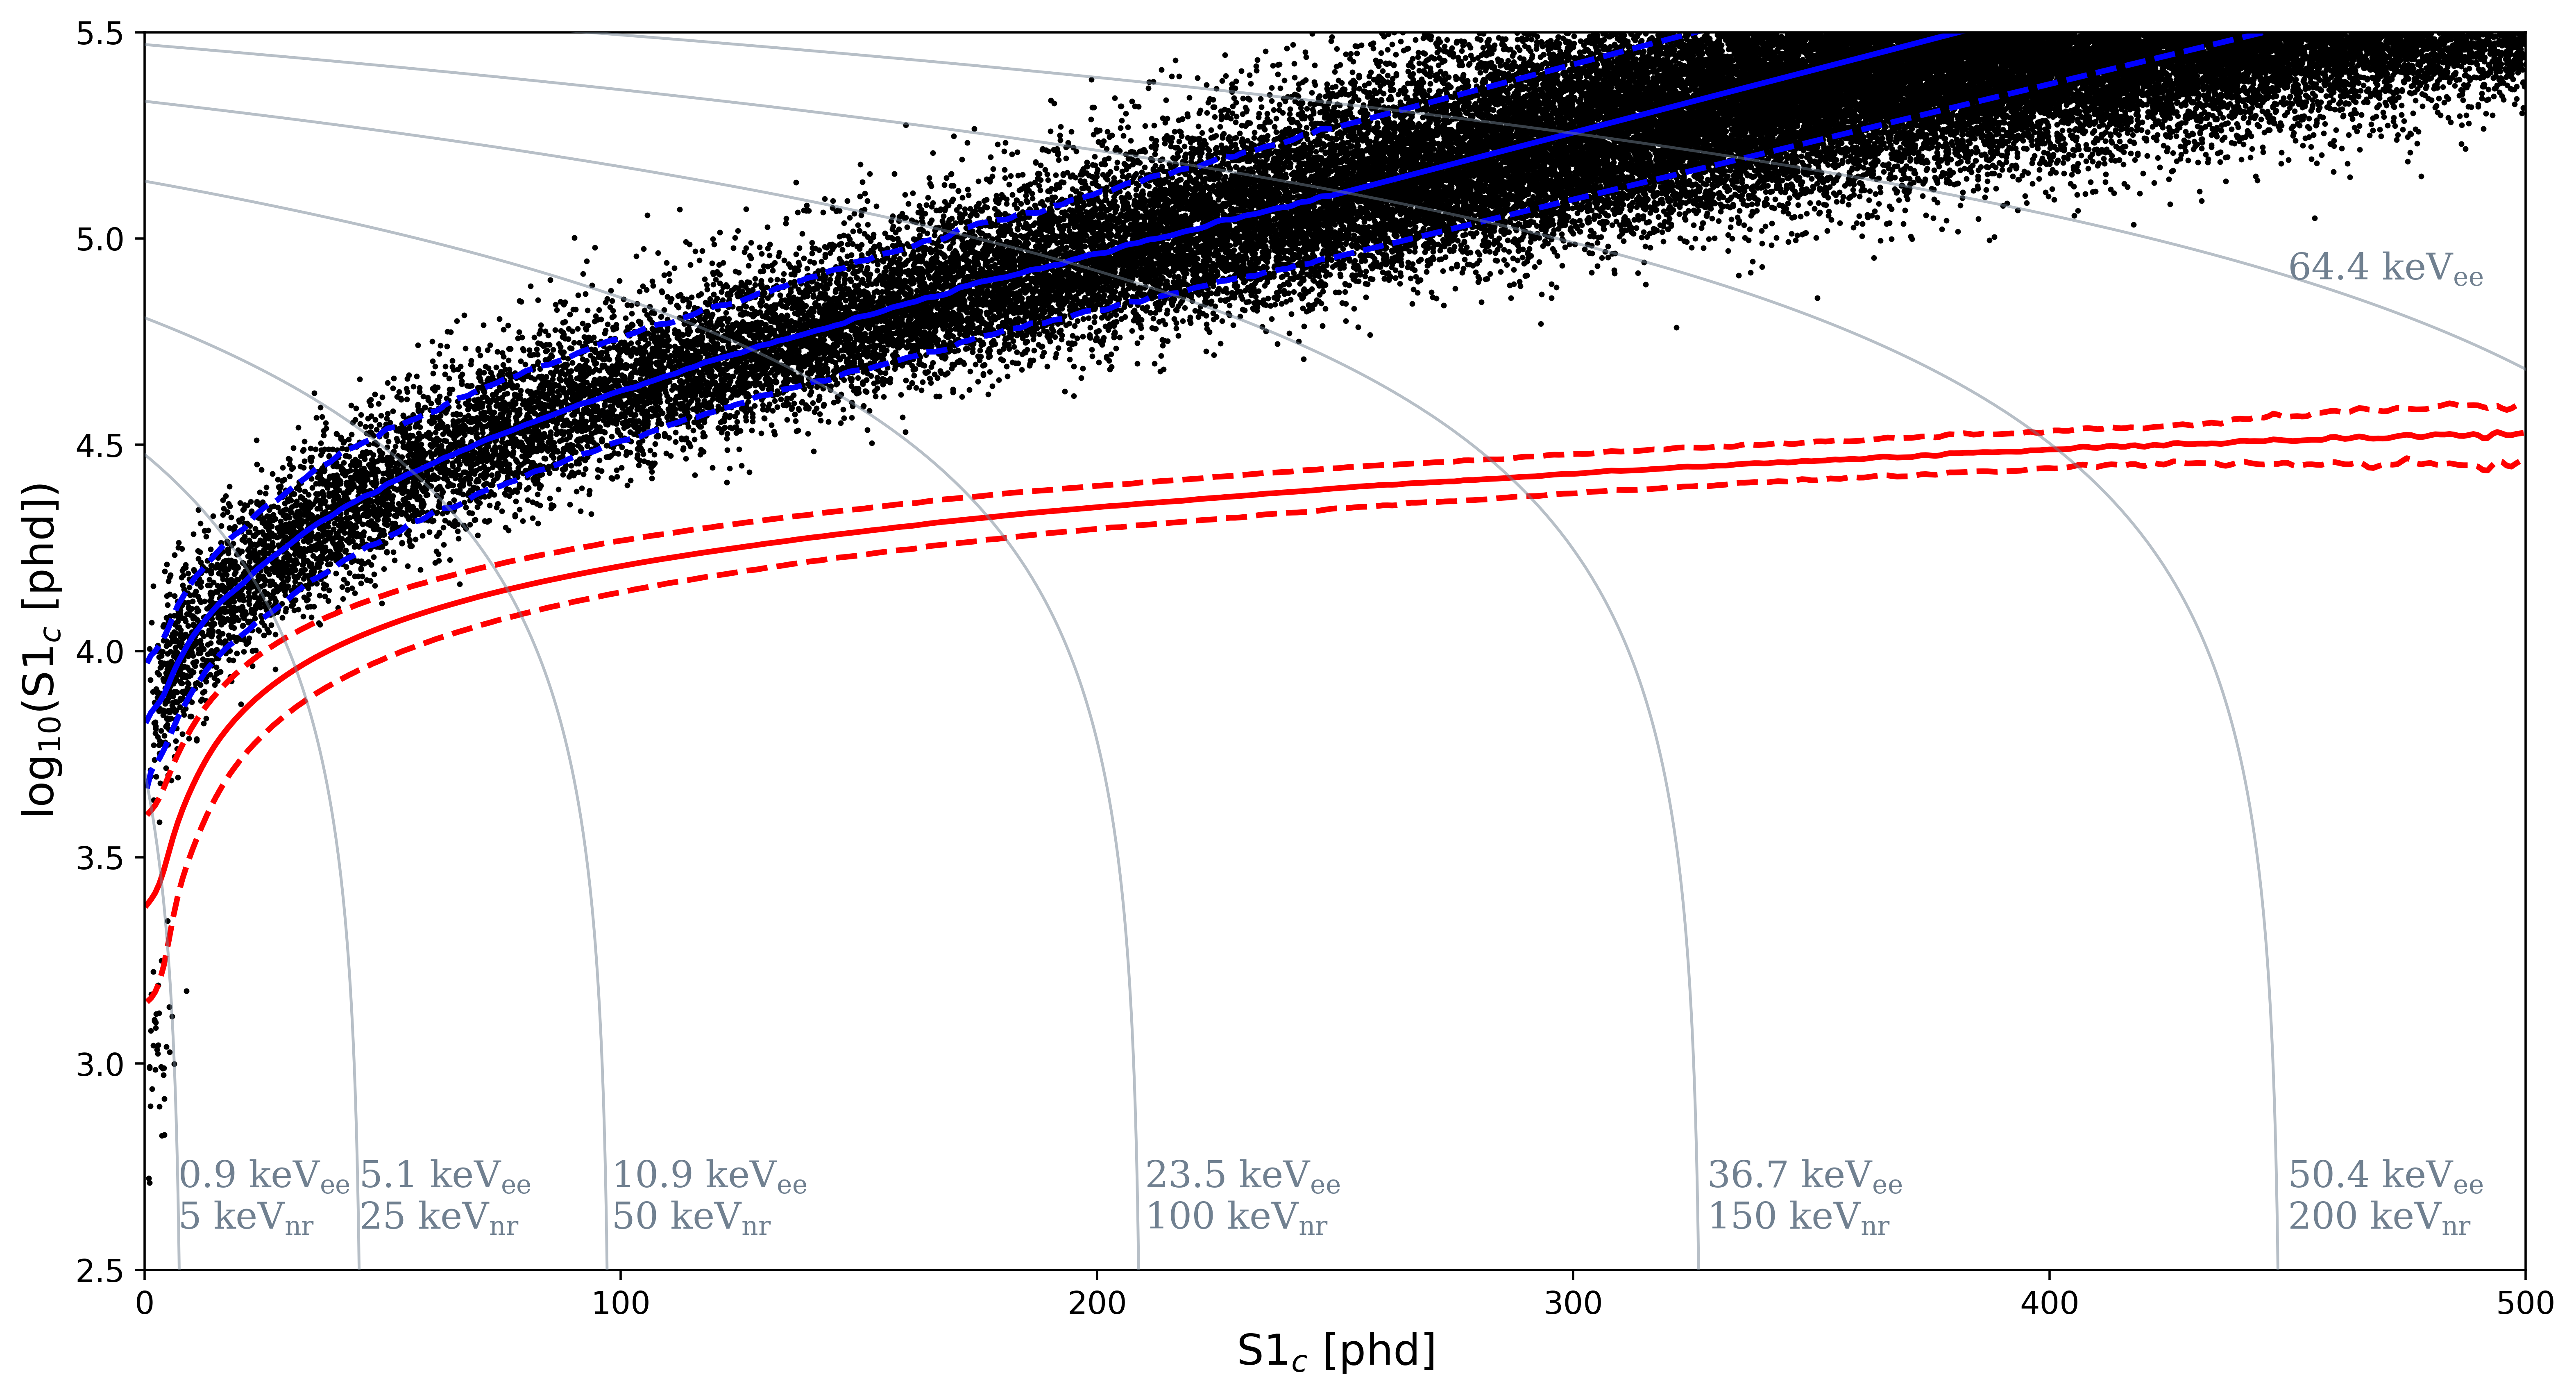
\includegraphics[width=15cm]{Figures/EFT/Projected_backgrounds/projected_backgrounds_s1_s2.png}
    \caption{Simulated data set for a background-only 1000 live day run with a 5.6 tonne fiducial mass. The ER and NR bands are shown in blue and red respectively; the solid lines are the mean and the dashed are 10\% and 90\% quantiles.}
    \label{fig:my_label}
\end{figure}







\subsection{Signal Model}
\par
\par
Both of the analyses were performed in the isoscalar basis as it allows for comparion to both LUX and XENON collraboration results.
More specifically, only the isoscalar basis was considered, with isovector interactions neglected.
\par
The case of 

\begin{equation}
    \frac{dR}{dE_R} = \frac{c^{a^2}_i \rho_\chi}{32 \pi m^3_\chi m^2_N} \int_{v_min} \frac{f(\vec{v}}{v} F^{a,a}_{i,i} (v^2, q^2) d^3 v
\end{equation}

\par
The recoil spectra were generated using \textit{DMFormFactor}.
This was chosen over the other software options mentioned in \autoref{sec:eft_theory} as it is the same as is used by the LUX, Panda-X and XENON collaborations.
Two different version of the codebase were used.
For the projected sensitivity, the recoils generated were from \textit{DMFormFactor} v6.0 which are the same version as those used in the published LUX and XENON100 results.
For the SR1 result, a newer, but unpublished version of \textit{DMFormFactor} was used\footnote{unpublished at time of writing}.
This has updated form factors, more accurately modelling the nuclei.
The recent publication on $\mathcal{L}$ by Panda-X used this version \cite{pandax_2_eft_ref}.
For a selection of operators the difference between the resultant form factors is shown in XXX.
The change in the resultant Bessel functions alter the shape of the recoils.

The WIMP signal model parameters used are shown in \autoref{tab:DMFormFactor_parameters}.
Recoil spectra out to 1000 keV for each operator were generated.

\begin{table}[]
    \centering
    \begin{tabular}{c|c}
        Parameter         & Value  \\ \hline
        $\nu_0$           & 220$km s^{-1}$ \\
        $\nu_{esc}$       & 544$km s^{-1}$ \\
        $\rho_{\chi}$     & 0.3 $GeV/cm^{3}$ \\
        $|\nu_E|$         & 245 $km s^{-1}$ 
    \end{tabular}
    \caption{DMFormFactor parameters used for the standard halo model. CITE XXX}
    \label{tab:DMFormFactor_parameters}
\end{table}
To improve the realism of the recoil and to maintain consistency with previous experiments the natural abundance of Xe isotopes were folded in.
Each operator was generated out to 1000 keV and in the isoscalar basis and a selection of the resultant differential rates are shown in \autoref{fig:HENR_Spin_Recoil_Spectrum}.
Each Operator was performed for a WIMP mass of [5, 7, 10, 12, 14, 21, 33, 50, 100, 200, 400, 1000, 4000] GeV.


\par
These were then used with the detector model to produce our observable quantities: \{$S1_c,log(S2_c)$\}, a selection of which are shown in FIGURE XXX.

%\input{Chapters/Analysis_EffectiveFieldTheory/Figures/Projected/signal_pdfs}


\subsection{Limits}
\par
Presented in \autoref{fig:EFT_Result_Projected_Sensitivity_1} and \autoref{EFT_Result_Projected_Sensitivity_2} are the limits from a one-sided PLR test statistic.
This was chosen over using a two-sided test as the purpose is to determine the sensitivity of LZ to the couplings, $c^{a}_i$, not the discovery significance. 
This approach is also in line with that used for the vanilla WIMP projected sensitivity \cite{LZ_projected_sensitivity_paper_ref} and other sensitivity studies within LZ \cite{LZ_Ibles_LZStats_Thesis_ref, umituktu_thesis_ref}.
\par
Included in the figures are the XENON100 \cite{xenon100_eft_ref} and LUX \cite{LUX_RUN4_EFT_2021} limits.
The parameter space which the LZ detector is a significant step forward compared to current limits.
The planned LZ exposure is orders of magnitude greater than the both LUX and XENON100 results, with 5.6 tonnes $\times$ 1000 live days for LZ compared to 34 kg $\times$ 224.6 live days with XENON100 and 100 kg $\times$ 311.2 live days for LUX.

$c^a_i$ has dimensional of mass$^{-2}$ which is 

The upper limits are shown in \autoref{fig:EFT_Result_Projected_Sensitivity_1} and \autoref{EFT_Result_Projected_Sensitivity_2}.
Note that the limit is presented in terms of the dimensionless values $({c}^{s}_{i}\times{m}^{2}_{w})^{2}$ rather than just $({c}^{s}_{i}$ (which has dimensionality of [mass]$^{-2}$, where $m_w$ is the Higg's vacuum expectation value.
This decision has been made due to several experiments making the decision to present them in this way (starting with XENON100 \cite{xenon100_eft_ref}).
\par
A key benefit of presenting in this manor is that it allows for a direct comparison to previous results which have been included in the limits shown.
Only a single data point is shown from LUX as their analysis was originally done in an \{$n,p$\} basis \cite{LUX_RUN4_EFT_2021}, and given the huge quantity of work it took they decided to reduce the problem to a single WIMP mass per operator.
\par
LZ has the potential to make significant strides in this region of parameter space which can be interpreted as 

\input{Chapters/Analysis_EffectiveFieldTheory/Figures/Projected/projected_limits_result}


%\section{LZ MDC3}
\par
Mock-Data Challenge 3 was the third and final simulation campaign prior to the availability of real data.
This campaign was designed to test the entirety of analysis framework to ensure data-readiness.

\par
As this simulation dataset was performed before the availability of real-data naturally some of the detector parameters used in the simulation are wrong.

\par
Something about PdfMaker being used

\subsection{Backgrounds}
\par
For this, PdfMaker was used for both backgrounds and signal.
Additionally, fewer backgrounds were taken into consideration and some simplifications were made.
Billy has more details on this though...

\subsection{Limits}
\par


\subsection{Discussion}

%\section{Results from First Science Run}
\par
In this section limits are placed on the elastic EFT operator couplings using data from the LZ's first science run (SR1).
The vanilla WIMP region of interest is considered here rather than an extended one as extending the region of interest would have resulted in a delay to this thesis.
An analysis for SI and SD dark matter interactions have already been performed in this recoil energy range, with null results \cite{lz_ws_sr1_ref}.
As this is the same dataset and cuts only a limited summary of the SR1 is presented here.
An overview of the calibration sources used for SR1 are described in \autoref{sec:lz_calibrations}.
A more complete description of the backgrounds in SR1 are laid out in \cite{lz_sr1_backgrounds_ref}.
All plots shown in this section except the signal models and limits originate from collaborators from within LZ and are not the authors own work.

\subsection{Overview of SR1}
\par
SR1 ran for a total of 116 days from 23 December 2021 to 18 April 2022 during which time the detector was in a stable running state.
During this period, several breaks occurred for both calibration runs and system maintenance reducing the data set down to 89 live days.
The length of time running was driven by a requirement to demonstrate physics capability and so only ran until the sensitivity to SI interactions was comparable to previous experiments.
SR1 was primarily an engineering run, and as such no blinding or salting of the data set was performed, as with any new detector there are unexpected features that are best understood by being able to see and explore them.
In order to mitigate bias in analysis development, analysis cuts were developed in side bands and from calibration data.

\subsection{TPC Calibration}
\par
The spacial variation in $S1$ and $S2$ were corrected using primarily internal sources which are naturally dispersed throughout the detector volume.
${}^{83m}$Kr and ${}^{131m}$Xe were used for this along with injected tritium (injected as tritiated methane CH$_3$T).
Energy calibrations were performed with the internal sources as well and also used ${}^{129m}$Xe which is monoenergetic at higher energies outside of the region considered here.
$g_1$ was determined to be 0.114$\pm$0.002 phd/photon and $g_2$ as 47.1$\pm$1.1 phd/electron.
The size of a single electron was measured as 57.6$\pm$1.9 phd/electron which gives an electron extraction efficiency of 80.5$\pm$3.7\%.
For calibrating the detector model, NR events were produced produced using the DD neutrons and AmLi, whilst ER events were produced using tritium.
The detector response was tuned to these measurements which are shown in \autoref{fig:sr1_tpc_calibration} along with the ER and NR bands.
\begin{figure}
    \centering
    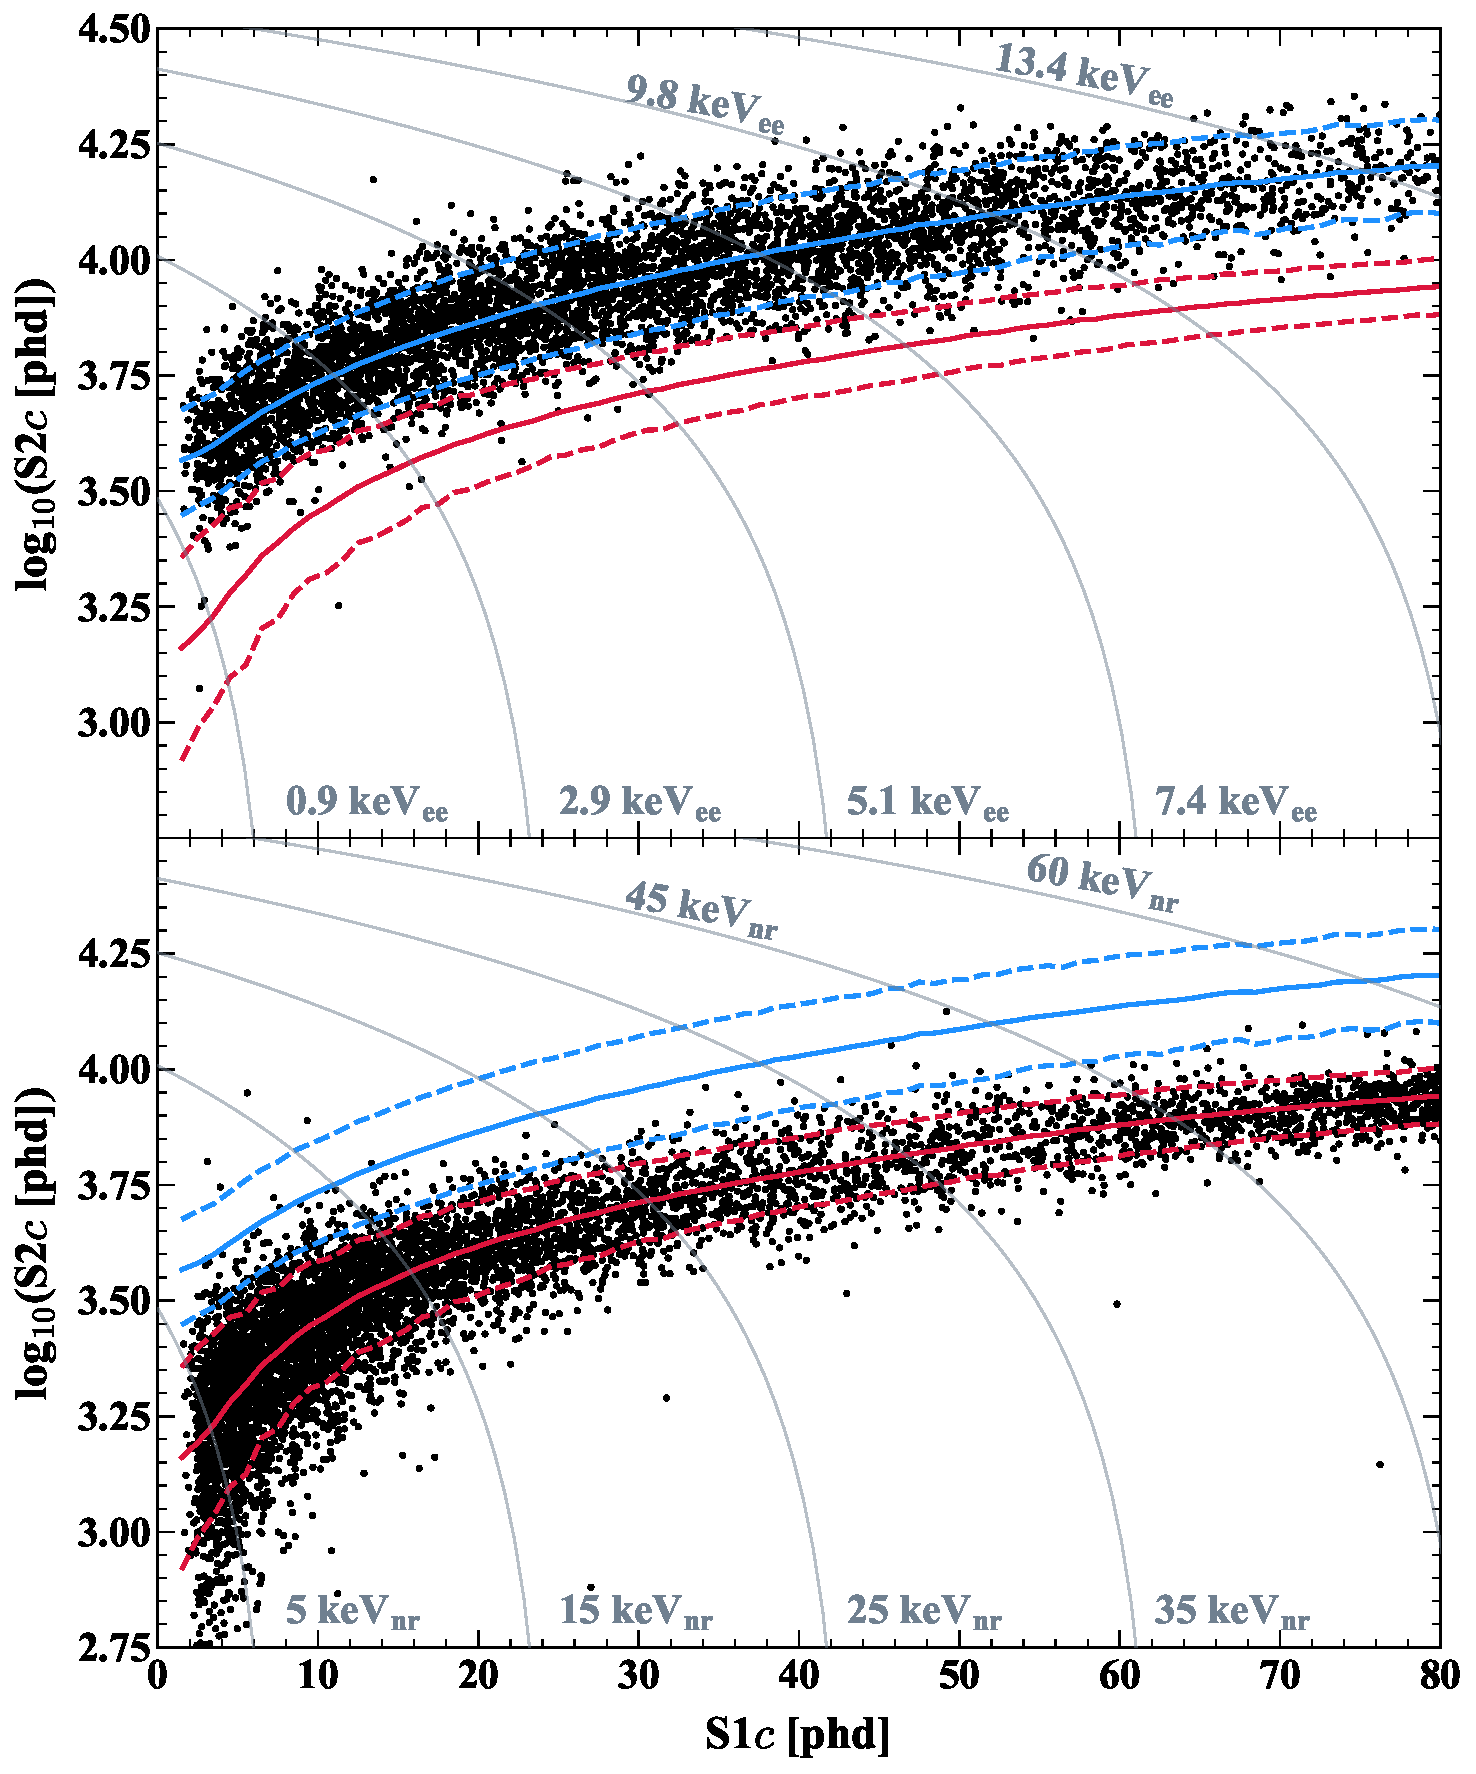
\includegraphics[width=10cm]{Figures/EFT/All_SR1_Plots/SR1WS_calOnly_0629_twoPanel.pdf}
    \caption{Calibration of ER and NR bands, shown in blue and red respectively.
             The solid line is the median and the dashed are the 10\% and 90\% quantiles.
             \textbf{Top:} ER events produced by $\beta$-decays from injected CH$_3$T.
             \textbf{Bottom:} NR events produced by DD neutrons.
             }
    \label{fig:sr1_tpc_calibration}
\end{figure}

\subsection{Analysis Cuts}
\par
In addition to the core-cuts that remove scatters that are inconsistent with dark matter that have been previously discussed, a multitude of other cuts were developed.
They fall broadly into three categories: live time, S2-based cuts and S1-based cuts.
These three, along with the core cuts are briefly discussed below.

\subsubsection{live time cuts}
The live time cuts are named as such as they have a large adverse affect on the amount of data that is uncharacteristic due to the high rate of pulses observed.
The two most significant cuts were an electron-train cut and a hot spot cut, together removing 35\% of the livetime.
After a large S2 event, a period of a sustained high rate is observed. 
This is due to electrons attaching to impurities and then being released at some later time, causing a delayed extraction and an elevated rate after the S2.
Single photons are also observed after the same event which is thought to be from delayed fluorescence.
The removal of time after an S2 until the detector rate settles corresponds to 29.8\% of live day loss.
Occasionally hot spots appeared in the TPC due to electron emission from the grids. 
These periods of time lasted approximately an hour at a time and reduced the live time by 6.6\%.
There were several other cuts in this category which combined livetime by a future 1\%.

\subsubsection{S2 cuts}
A suite of cuts were developed to remove S2s which did not look like an S2 should if it had originated from a LXe scatter.
These targeted accidental events.

\subsubsection{S1 cuts}


developed a hot spot where 

\subsubsection{Core cuts}
All of these core cuts focus on removing clean scatters in the TPC, but which do not match the properties of dark matter.
Only events with a single S1-S2 pulse pair are selected, multiple S1 or multiple S2 events are removed.
\par
The fiducial region was defined in $z$ by the drift time (time between the S1 and S2 pulses) of between [86,936.5] $\mu$s which corresponds to approximately 12.8 cm below the gate grid and 2.2 cm from the cathode grid.
$r$ was defined as either [4.0,5.0,5.2] cm from the TPC wall. The variation in the $r$ is to remove regions where the electric field is non-uniform, and effects from being close to the wall.
Within this region a the volume of xenon is 5.5$\pm$0.2 tonnes.
\autoref{fig:sr1_fiducial_cut} shows the fiducial volume definition.
\par
The region of interest was defined as 3 phd $<$ S1$_c <$ 80 phd, S2 $>$ 600 phd and S2$_c <$ 10$^5$ phd.
\par
The OD veto window was set to the value discussed in the previous chapter of 1200 $\mu$s, with an energy threshold of 200 keV.
The Skin veto window was set to 400 $\mu$s.
Additionally a prompt veto window was implemented to remove events where the S1 is within [-300,300] ns of a pulse in either the Skin or OD.

\par
The combined efficiency of all of these cuts is shown in \autoref{fig:sr1_nr_efficiency}.
The efficiency in the ROI was determined using AmLi and tritium data.
A total of 335 events remained after the application of all of these cuts.

\begin{figure}
    \centering
    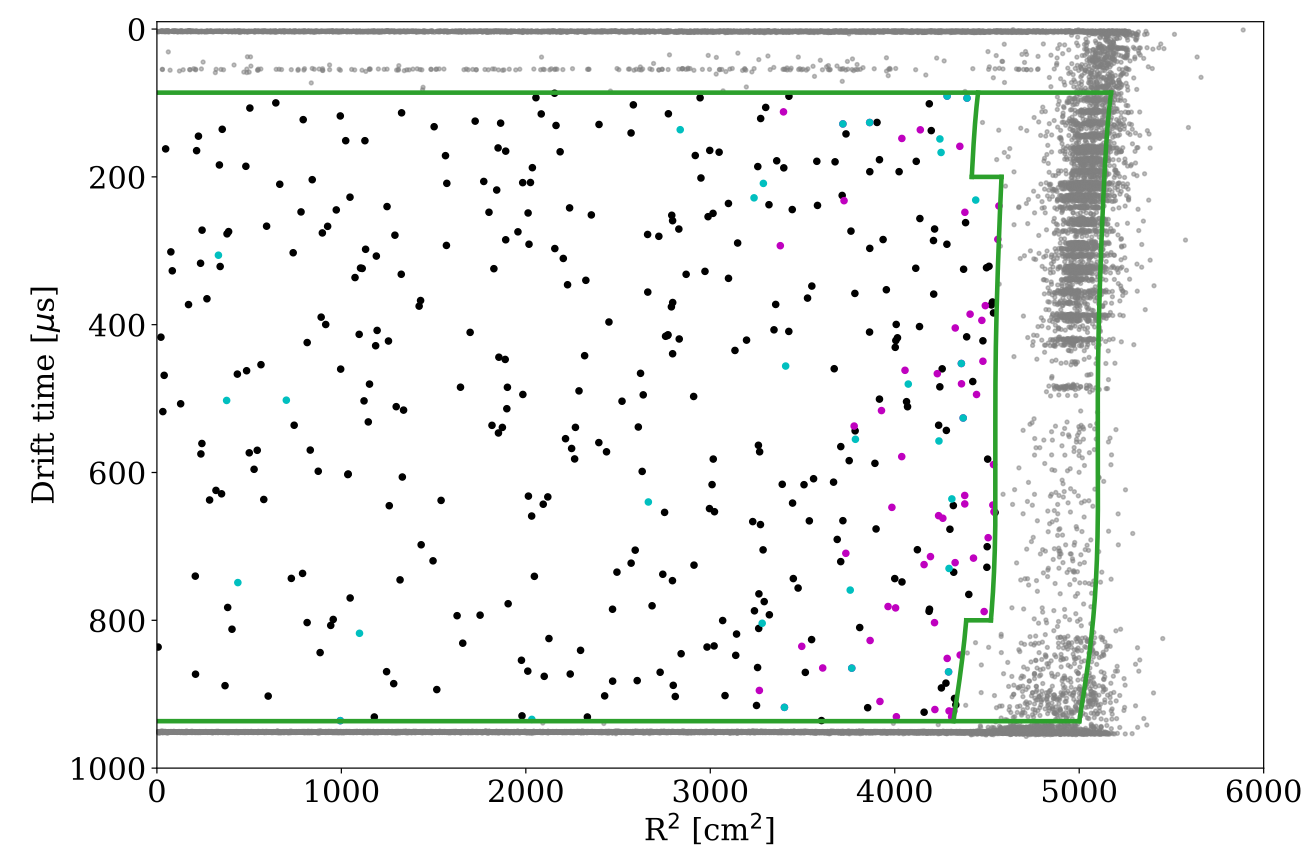
\includegraphics[width=15cm]{Figures/EFT/All_SR1_Plots/fid.png}
    \caption{Distribution of events in the SR1 dataset in the ROI.
    The vertical green line which two steps is the fiducial region.
    The other green line shown is the wall definition.
    The events in grey are outside of the fiducial volume and so vetoed. 
    The events marked in cyan were removed by the OD and the events marked in purple by the Skin.
    The remaining events in the WIMP dataset are shown in black.}
    \label{fig:sr1_fiducial_cut}
\end{figure}

\begin{figure}
    \centering
    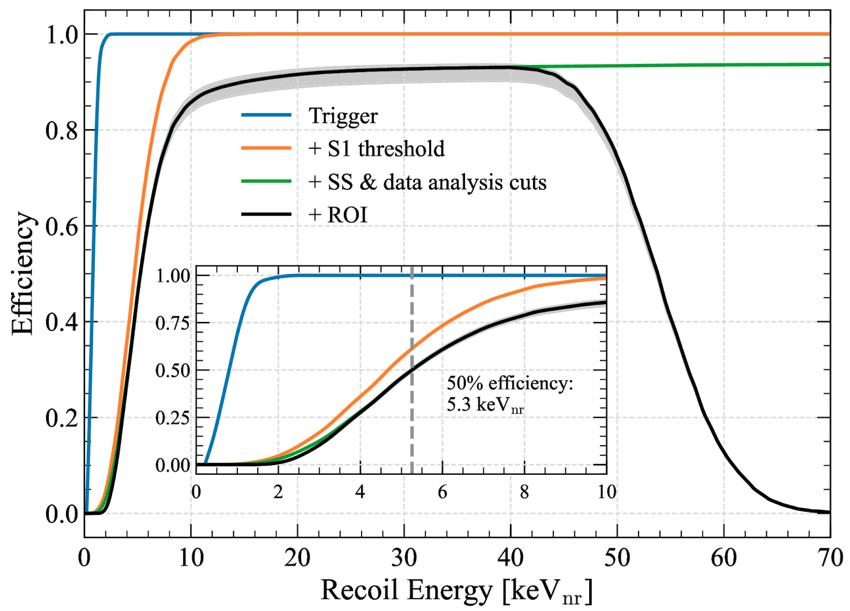
\includegraphics[width=10cm]{Figures/EFT/All_SR1_Plots/NR_efficiency.png}
    \caption{Signal efficiency as a function of NR energy for the trigger (blue), S1 threshold (orange), all analysis cuts expect ROI (green) and the ROI (black).
    The vertical dashed line is the the 50\% efficiency point.
    }
    \label{fig:sr1_nr_efficiency}
\end{figure}

\subsection{Background Model}
\par
In the background model, 9 components were included.
The grouping is based upon the distribution in the ROI and the level of uncertainty.

\par
The ${}^{222}$Rn chain and ${}^{220}$Rn chain both produce flat $\beta$ contribution.
The rate of these was determined via $\alpha$-peak fitting to the ER band outside of the ROI which can be seen in \autoref{fig:sr1_spectra}
The $\gamma$ spectrum from the detector contaminants is also flat in this region.
These contributions are treated as a single background labelled $\beta$ decays + Det. ER.
This is the largest contribution to the expected rate, with 218 $\pm$ 36 events.

The rate of detector 
\begin{figure}
    \centering
    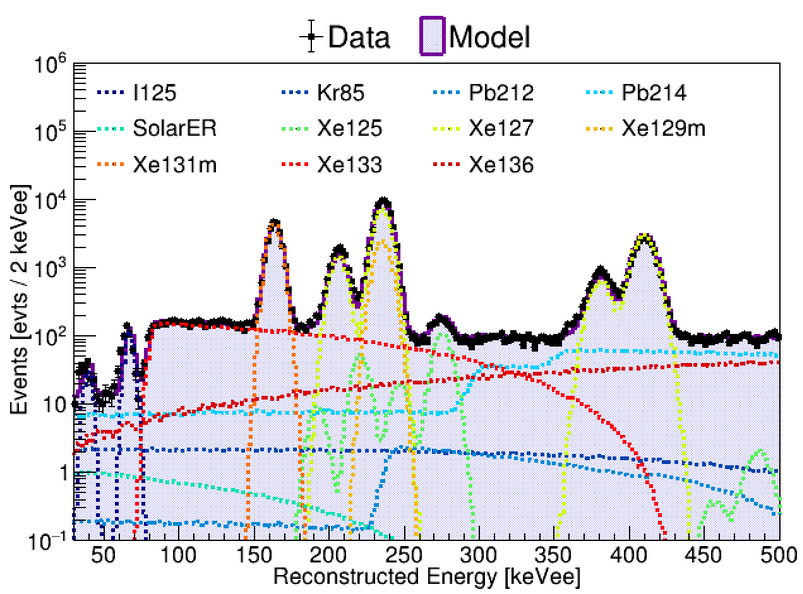
\includegraphics[width=10cm]{Figures/EFT/All_SR1_Plots/ER_band_fit.png}
    \caption{SR1 vanilla WIMP-search data (black points) overlaid on the background model.
    The contours shown for each distribution are 1 and 2 $\sigma$.
    ${}^{8}$B is shown in green, ${}^{37}$Ar is shown in orange, the combined ER spectrum in grey.
    The red lines are the NR band with the medium, 10\% and 90\% quantiles.
    The distribution from a 30 GeV WIMP is also shown in purple. 
    }
    \label{fig:sr1_spectra}
\end{figure}


\par
Solar neutrinos which also produce a flat contribution are not included as the rate is more finely constrained \cite{pp_solar_neutrinos_rate_ref}.
\par
Decays from three Xenon isotopes were included.
${}^{127}$Xe and ${}^{124}$Xe contribute to the ER spectrum by double electron capture and double $\beta$ decay respectively.
The rates of these are constrained by know abundances \cite{xenon_isotopes_ref}.
\par
Two interesting backgrounds considered here is weren't considered in the projected case are ${}^{37}$Ar and ${}^{127}$Xe.
These are both short-lived isotopes, with half-lives of 35 days and 36.3 days respectively.
They appear due to cosmogenic activation of the xenon when the xenon is at the surface level\footnote{of the mine. Not the surface of the LXe.}.
Once underground these components decay away and so are not of concern in future data runs.
The rates are therefore constrained by the delivery schedule of the xenon into the Davis cavern \cite{lz_argon37_ref}.
There are expected to be $\approx$100 ${}^{37}$Ar events in this data set but there a very large uncertainty meaning that it could be has high at 300.

\par
The two NR contributions considered are from ${}^{8}$B solar neutrinos and neutrons from the detector.
There are expected to be 0 detector neutrons in this dataset, a value constrained by the radioassay of the detector components prior to construction \cite{LZ_assay_ref}.

\par
The expected contribution from each component in the model is \autoref{tab:sr1_ws_lz_backgrounds}.
The uncertainties on the values shown indicate the constraints placed on each component during the PLR.

\begin{table}[]
    \centering
    \begin{tabular}{c|c}
        Background Component     & Expected Number of Events  \\ \hline
        $\beta$ decays + Det. ER & 218 $\pm$ 36 \\
        $\nu$ ER                 & 27.3 $\pm$ 1.6 \\
        ${}^{127}$Xe             & 9.3 $\pm$ 0.8 \\
        ${}^{124}$Xe             & 5.0 $\pm$ 1.4 \\
        ${}^{136}$Xe             & 15.2 $\pm$ 2.4 \\
        ${}^{8}$B CE$\nu$NS      & 0.15 $\pm$ 0.01 \\
        Accidentals              & 1.2 $\pm$ 0.3 \\
        ${}^{37}$Ar              & [0, 291]      \\
        neutrons                 & 0.0${}^{+0.2}$
    \end{tabular}
    \caption{Expected number of events from each component in the background model.}
    \label{tab:sr1_ws_lz_backgrounds}
\end{table}

\par
The best-fit background model is shown in \autoref{fig:final_data_points} with the the data set overlaid.
The best-fit values were identical to the SI result, as such the plot is shown from the SI result \cite{lz_ws_sr1_ref}.
The WIMP contours (shown in purple) are for a 30 GeV/c${^2}$ which is analogous to $\Operator$1 interactions of the same mass.

\begin{figure}
    \centering
    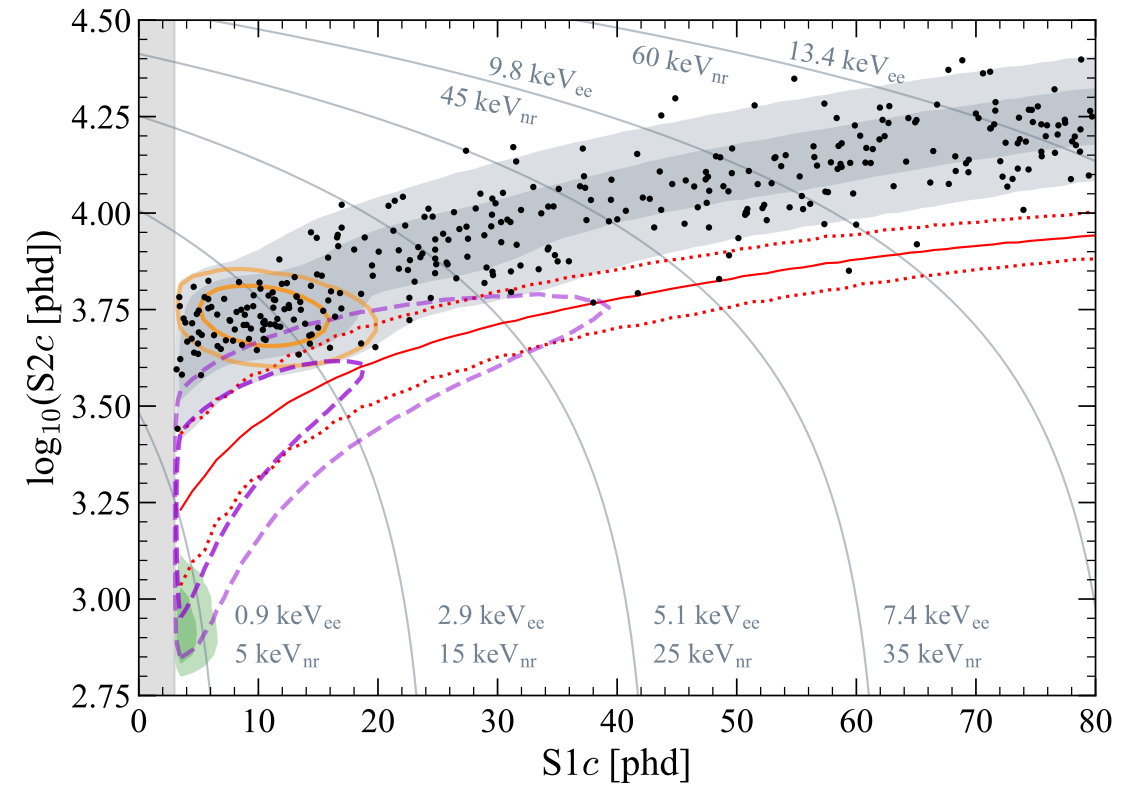
\includegraphics[width=10cm]{Figures/EFT/All_SR1_Plots/final_data_points.png}
    \caption{SR1 vanilla WIMP-search data (black points) overlaid on the background model.
    The contours shown for each distribution are 1 and 2 $\sigma$.
    ${}^{8}$B is shown in green, ${}^{37}$Ar is shown in orange, the combined ER spectrum in grey.
    The red lines are the NR band with the medium, 10\% and 90\% quantiles.
    The distribution from a 30 GeV WIMP is also shown in purple. 
    }
    \label{fig:final_data_points}
\end{figure}

\subsection{Signal Model}
\par
Unlike the projected sensitivity, this analysis used the recommended astronomic properties laid out in \cite{standard_halo_model_conventions_ref}.
These are summarised in \autoref{tab:sr1_DMFormFactor_parameters}.
Of particular note is the increased velocity of the WIMP velocity.
The impact of this on a selection of operator differential recoil rates is shown in FIGURE XXX.
\par
The increased velocity of the dark matter increased the flux, and therefore expected rate of recoils.
As the expected signal rate increases, the lack of seeing a signal then sets a tighter constraint on the WIMP-nucleon scattering.
A more complete comparison between how uncertainties in the standard model parameters affect sensitivity to dark matter searches can be found in \cite{LZ_Ibles_LZStats_Thesis_ref,billyboxer_thesis_ref}.

\begin{table}[]
    \centering
    \begin{tabular}{c|c}
        Parameter         & Value  \\ \hline
        $\nu_0$           & 238$km s^{-1}$ \\
        $\nu_{esc}$       & 544$km s^{-1}$ \\
        $\rho_{\chi}$     & 0.3 $GeV/cm^{3}$ \\
        $|\nu_E|$         & 245 $km s^{-1}$ 
    \end{tabular}
    \caption{Standard Halo Model parameters used for SR1 sensitivity study.}
    \label{tab:sr1_DMFormFactor_parameters}
\end{table}


\subsection{Limits}
\par
On each operator for WIMP masses of [5, 7, 10, 12, 14, 21, 33, 50, 100, 200, 400, 1000, 4000] GeV/c$^2$, a 2-sided frequentist confidence interval is determined above a 90\% confidence level.
Presented in \autoref{fig:EFT_Result_Projected_Sensitivity_1} and \autoref{fig:EFT_Result_Projected_Sensitivity_2} are the limits, presented in the same dimensionless form as the projected limits.
Shown as before are the previous limits from both Xenon100 \cite{xenon100_eft_ref} and LUX \cite{LUX_RUN4_EFT_2021}.

%Consistent with the SI and SD search, a null result was found, setting limits on the operator couplings.
%These are shown in \autoref{fig:EFT_Result_Projected_Sensitivity_1} and \autoref{fig:EFT_Result_Projected_Sensitivity_2} in the same dimensionless scale as the projected limits.

\par
World-leading sensitivity has been achieved for all operators at at least some masses.
In several cases, such as $\Operator$6 the sensitivity of LZ is less than that of both LUX and XENON100. 
This is due to the recoil distributions of these operators peaking outside of the ROI used here for high WIMP masses.
Despite this reduced parameter space, the huge increase in exposure has made LZ very competitive.

\input{Chapters/Analysis_EffectiveFieldTheory/Figures/WIMP_Search/final_dataset_events}

For SR1 fewer parameters were taken into consideration with the PLR working in [S1,logS2] space.
Increasing the set of parameters will allow for improved discrimination and a potential discovery but runs into significant computational limitations as discovered in both \cite{nicolelarsen_thesis_ref, shaunalsum_thesis_ref, billyboxer_thesis_ref}, a different approach such as that described in \cite{flamenest_ref} and \cite{lux_ml_plr_ref} offer some hope for this.

\input{Chapters/Analysis_EffectiveFieldTheory/Figures/WIMP_Search/ws_limits}

For SR1 fewer parameters were taken into consideration with the PLR working in [S1,logS2] space.
Increasing the set of parameters will allow for improved discrimination and a potential discovery but runs into significant computational limitations as discovered in both \cite{nicolelarsen_thesis_ref, shaunalsum_thesis_ref, billyboxer_thesis_ref}, a different approach such as that described in \cite{flamenest_ref} and \cite{lux_ml_plr_ref} offer some hope for this.

%\chapter{Conclusion}
\label{chap:conclusion}
\par
The source of the unknown mass of the universe remains a mystery.
The particle interpretation remains the most favoured, with WIMPs at the forefront.
\par
The LZ collaboration has constructed the most sensitive direct detection dark matter experiment, setting world-leading constraints on spin-independent and spin-dependent cross-sections.
This has been achieved using a xenon time projection chamber (TPC), two veto detectors and a strong understanding of the backgrounds in each detector.

\par
The simulation challenge of being able to properly simulate all backgrounds completely remains a difficult task.
A solution to optical simulations was presented in \autoref{chap:lz_simulations}, using GPUs, showing an improvement of in excess of 700 times that is achievable by CPU simulations.
In future, the method described can be extended to all parts of the simulation chain and particles one may wish to simulate.

\par
The Outer Detector (OD), which surrounds the TPC, acts to veto neutron events.
Measured in simulation in \autoref{chapter:lz_outer_detector} and in data in \autoref{chap:analysis_of_the_od}, it was found that it has not met the performance requirements it was designed for.
The neutron veto efficiency was measured during the commissioning phase as 84.6$\pm$1.2\%.
The decrease compared to simulations is believed to be from water saturation of foam, causing neutrons to take longer to reach the OD, and a fraction to never reach it.
\par
The backgrounds expected in the OD were also examined in both simulation and data.
The observed rate above 200 keV was lower than expected.
An unexpectedly high rate of ${}^{210}$Po was observed which is believed to be as a result of the acrylic tanks of the OD being open to the cavern air underground for prolonged periods of time, causing plate-out.
A fit to the background spectra was performed with the largest contribution from cavern-$\gamma$ events.

\par
Two analyses of non-relativistic EFT operator WIMP-nucleon couplings were presented in \autoref{chap:analysis_eft_work}.
A projected sensitivity of LZ from a 1000 live-day exposure to these signal models was performed using an extended region of interest.
It was shown that LZ will be able to probe 4 orders of magnitude lower than previous limits.
A search was performed on the first science run data of LZ in a limited region of interest.
This set world-leading exclusion constraints on all EFT operator couplings at almost all WIMP masses probed.
With an extended region of interest, LZ will be able to increase sensitivity to all WIMP masses.

\par
LZ is still in its infancy, having completed a 60 live-day WIMP search of a planned 1000 live-day search.
This is an increase in exposure of nearly 17 times.
The possibility of detecting a WIMP with LZ remains.
These are exciting times for direct dark matter detection.



%\chapter{Playground}

\clearpage
\newcommand{\nodewidth}{1cm}
\newcommand{\textnodewidth}{0.2cm}
\newcommand{\nodeminimumwidth}{32pt}
\newcommand{\nodespacing}{10pt}


\begin{landscape}
\begin{figure}
    \centering
\begin{tikzpicture}
  [node distance=0.05cm,text centered, thick]
  \tikzstyle{every node}=[font=\fontsize{5}{5}\selectfont]
 
    % For 3 chains, need 13 across
 \node[draw, rectangle, inner sep=0pt, text width=\nodewidth, minimum height=0.1cm, minimum width=\nodeminimumwidth, ] (neptunium_node_minus1) {};   
 \node[draw, rectangle, inner sep=0pt, text width=\nodewidth, minimum height=0.1cm, minimum width=\nodeminimumwidth, right=of neptunium_node_minus1] (neptunium_node_0) {};
 \node[draw, rectangle, inner sep=0pt, text width=\nodewidth, minimum height=0.1cm, minimum width=\nodeminimumwidth, right=of neptunium_node_0] (neptunium_node_1) {};
 \node[draw, rectangle, inner sep=0pt, text width=\nodewidth, minimum height=0.1cm, minimum width=\nodeminimumwidth, right=of neptunium_node_1] (neptunium_node_2) {};
 \node[draw, rectangle, inner sep=0pt, text width=\nodewidth, minimum height=0.1cm, minimum width=\nodeminimumwidth, right=of neptunium_node_2] (neptunium_node_3) {};
 \node[draw, rectangle, inner sep=0pt, text width=\nodewidth, minimum height=0.1cm, minimum width=\nodeminimumwidth, right=of neptunium_node_3] (neptunium_node_4) {};
 \node[draw, rectangle, inner sep=0pt, text width=\nodewidth, minimum height=0.1cm, minimum width=\nodeminimumwidth, right=of neptunium_node_4] (neptunium_chain_sep_1) {};
 \node[draw, rectangle, inner sep=0pt, text width=\nodewidth, minimum height=0.1cm, minimum width=\nodeminimumwidth, right=of neptunium_chain_sep_1] (neptunium_node_5) {};
 \node[draw, rectangle, inner sep=0pt, text width=\nodewidth, minimum height=0.1cm, minimum width=\nodeminimumwidth, right=of neptunium_node_5] (neptunium_node_6) {};
 \node[draw, rectangle, inner sep=0pt, text width=\nodewidth, minimum height=0.1cm, minimum width=\nodeminimumwidth, right=of neptunium_node_6] (neptunium_node_7) {};
 \node[draw, rectangle, inner sep=0pt, text width=\nodewidth, minimum height=0.1cm, minimum width=\nodeminimumwidth, right=of neptunium_node_7] (neptunium_node_8) {};
 \node[draw, rectangle, inner sep=0pt, text width=\nodewidth, minimum height=0.1cm, minimum width=\nodeminimumwidth, right=of neptunium_node_8] (neptunium_node_9) {};
 \node[draw, rectangle, inner sep=0pt, text width=\nodewidth, minimum height=0.1cm, minimum width=\nodeminimumwidth, right=of neptunium_node_9] (neptunium_chain_sep_2) {};
 \node[draw, rectangle, inner sep=0pt, text width=\nodewidth, minimum height=0.1cm, minimum width=\nodeminimumwidth, right=of neptunium_chain_sep_2] (neptunium_node_10) {};
 \node[draw, rectangle, inner sep=0pt, text width=\nodewidth, minimum height=0.1cm, minimum width=\nodeminimumwidth, right=of neptunium_node_10] (neptunium_node_11) {};
 \node[draw, rectangle, inner sep=0pt, text width=\nodewidth, minimum height=0.1cm, minimum width=\nodeminimumwidth, right=of neptunium_node_11] (neptunium_node_12) {};
 \node[draw, rectangle, inner sep=0pt, text width=\nodewidth, minimum height=0.1cm, minimum width=\nodeminimumwidth, right=of neptunium_node_12] (neptunium_label_sep) {};
 \node[draw, rectangle, inner sep=0pt, text width=\nodewidth, minimum height=0.1cm, minimum width=\nodeminimumwidth, right=of neptunium_label_sep] (neptunium_sep_3) {};
    
 \node[circle, inner sep=0pt, text width=\nodewidth, minimum width=\nodeminimumwidth, below=of neptunium_node_minus1] (uranium_node_minus1) {};   
 \node[draw, circle, inner sep=0pt, text width=\nodewidth, minimum width=\nodeminimumwidth, below=of neptunium_node_0] (uranium_node_0) {${}^{234}_{92}$U $245e^{3}$y};
 \node[circle, inner sep=0pt, text width=\nodewidth, minimum width=\nodeminimumwidth, below=of neptunium_node_1] (uranium_node_1) {};
 \node[draw, circle, inner sep=0pt, text width=\nodewidth, minimum width=\nodeminimumwidth, below=of neptunium_node_2] (uranium_node_2) {${}^{238}_{92}$U $4.5e^{9}$y};
 \node[circle, inner sep=0pt, text width=\nodewidth, minimum width=\nodeminimumwidth, below=of neptunium_node_3] (uranium_node_3) {};
 \node[circle, inner sep=0pt, text width=\nodewidth, minimum width=\nodeminimumwidth, below=of neptunium_node_4] (uranium_node_4) {};
 \node[circle, inner sep=0pt, text width=\nodewidth, minimum width=\nodeminimumwidth, below=of neptunium_chain_sep_1] (uranium_chain_sep_1) {};
 \node[draw, circle, inner sep=0pt, text width=\nodewidth, minimum width=\nodeminimumwidth, below=of neptunium_node_5] (uranium_node_5) {${}^{235}_{92}$U $7.0e^{8}$y};
 \node[circle, inner sep=0pt, text width=\nodewidth, minimum width=\nodeminimumwidth, below=of neptunium_node_6] (uranium_node_6) {};
 \node[circle, inner sep=0pt, text width=\nodewidth, minimum width=\nodeminimumwidth, below=of neptunium_node_7] (uranium_node_7) {};
 \node[circle, inner sep=0pt, text width=\nodewidth, minimum width=\nodeminimumwidth, below=of neptunium_node_8] (uranium_node_8) {};
 \node[circle, inner sep=0pt, text width=\nodewidth, minimum width=\nodeminimumwidth, below=of neptunium_node_9] (uranium_node_9) {};
 \node[circle, inner sep=0pt, text width=\nodewidth, minimum width=\nodeminimumwidth, below=of neptunium_chain_sep_2] (uranium_chain_sep_2) {};
 \node[circle, inner sep=0pt, text width=\nodewidth, minimum width=\nodeminimumwidth, below=of neptunium_node_10] (uranium_node_10) {};
 \node[circle, inner sep=0pt, text width=\nodewidth, minimum width=\nodeminimumwidth, below=of neptunium_node_11] (uranium_node_11) {};
 \node[circle, inner sep=0pt, text width=\nodewidth, minimum width=\nodeminimumwidth, below=of neptunium_node_12] (uranium_node_12) {};
 \node[circle, inner sep=0pt, text width=\nodewidth, minimum width=\nodeminimumwidth, below=of neptunium_label_sep] (uranium_label_sep) {};
 \node[circle, inner sep=0pt, text width=\nodewidth, minimum width=\nodeminimumwidth, below=of neptunium_sep_3] (uranium_sep_3) {Uranium};

 \node[circle, inner sep=0pt, text width=\nodewidth, minimum width=\nodeminimumwidth, below=of uranium_node_minus1] (protactinium_node_minus1) {};
 \node[circle, inner sep=0pt, text width=\nodewidth, minimum width=\nodeminimumwidth, below=of uranium_node_0] (protactinium_node_0) {};
 \node[draw, circle, inner sep=0pt, text width=\nodewidth, minimum width=\nodeminimumwidth, below=of uranium_node_1] (protactinium_node_1) {${}^{234}_{91}$Pa $1.2$m};
 \node[circle, inner sep=0pt, text width=\nodewidth, minimum width=\nodeminimumwidth, below=of uranium_node_2] (protactinium_node_2) {};
 \node[circle, inner sep=0pt, text width=\nodewidth, minimum width=\nodeminimumwidth, below=of uranium_node_3] (protactinium_node_3) {};
 \node[circle, inner sep=0pt, text width=\nodewidth, minimum width=\nodeminimumwidth, below=of uranium_node_4] (protactinium_node_4) {};
 \node[circle, inner sep=0pt, text width=\nodewidth, minimum width=\nodeminimumwidth, below=of uranium_node_5] (protactinium_node_5) {};
 \node[draw, circle, inner sep=0pt, text width=\nodewidth, minimum width=\nodeminimumwidth, below=of uranium_node_6] (protactinium_node_6) {${}^{231}_{91}$Pa $3.3e^{4}$y};
 \node[circle, inner sep=0pt, text width=\nodewidth, minimum width=\nodeminimumwidth, below=of uranium_node_7] (protactinium_node_7) {};
 \node[circle, inner sep=0pt, text width=\nodewidth, minimum width=\nodeminimumwidth, below=of uranium_node_8] (protactinium_node_8) {};
 \node[circle, inner sep=0pt, text width=\nodewidth, minimum width=\nodeminimumwidth, below=of uranium_node_9] (protactinium_node_9) {};
 \node[circle, inner sep=0pt, text width=\nodewidth, minimum width=\nodeminimumwidth, below=of uranium_node_10] (protactinium_node_10) {};
 \node[circle, inner sep=0pt, text width=\nodewidth, minimum width=\nodeminimumwidth, below=of uranium_node_11] (protactinium_node_11) {};
 \node[circle, inner sep=0pt, text width=\nodewidth, minimum width=\nodeminimumwidth, below=of uranium_node_12] (protactinium_node_12) {};
 \node[circle, inner sep=0pt, text width=\nodewidth, minimum width=\nodeminimumwidth, below=of uranium_label_sep] (protactinium_label_sep) {};
 \node[circle, inner sep=0pt, text width=\nodewidth, minimum width=\nodeminimumwidth, below=of uranium_sep_3] (protactinium_sep_3) {Protactinium};

 \node[circle, inner sep=0pt, text width=\nodewidth, minimum width=\nodeminimumwidth, below=of protactinium_node_minus1] (thorium_node_minus1) {};
 \node[draw, circle, inner sep=0pt, text width=\nodewidth, minimum width=\nodeminimumwidth, below=of protactinium_node_0] (thorium_node_0) {${}^{230}_{90}$Th $75e^{3}$y};
 \node[circle, inner sep=0pt, text width=\nodewidth, minimum width=\nodeminimumwidth, below=of protactinium_node_1] (thorium_node_1) {};
 \node[draw, circle, inner sep=0pt, text width=\nodewidth, minimum width=\nodeminimumwidth, below=of protactinium_node_2] (thorium_node_2) {${}^{234}_{90}$Th $24.1$d};
 \node[circle, inner sep=0pt, text width=\nodewidth, minimum width=\nodeminimumwidth, below=of protactinium_node_3] (thorium_node_3) {};
 \node[circle, inner sep=0pt, text width=\nodewidth, minimum width=\nodeminimumwidth, below=of protactinium_node_4] (thorium_node_4) {};
 \node[draw, circle, inner sep=0pt, text width=\nodewidth, minimum width=\nodeminimumwidth, below=of protactinium_node_5] (thorium_node_5) {${}^{231}_{90}$Th $25.5$h};
 \node[circle, inner sep=0pt, text width=\nodewidth, minimum width=\nodeminimumwidth, below=of protactinium_node_6] (thorium_node_6) {};
 \node[draw, circle, inner sep=0pt, text width=\nodewidth, minimum width=\nodeminimumwidth, below=of protactinium_node_7] (thorium_node_7) {${}^{227}_{90}$Th $18.7$d};
 \node[circle, inner sep=0pt, text width=\nodewidth, minimum width=\nodeminimumwidth, below=of protactinium_node_8] (thorium_node_8) {};
 \node[circle, inner sep=0pt, text width=\nodewidth, minimum width=\nodeminimumwidth, below=of protactinium_node_9] (thorium_node_9) {};
 \node[draw, circle, inner sep=0pt, text width=\nodewidth, minimum width=\nodeminimumwidth, below=of protactinium_node_10] (thorium_node_10) {${}^{228}_{90}$Th $1.9$y};
 \node[circle, inner sep=0pt, text width=\nodewidth, minimum width=\nodeminimumwidth, below=of protactinium_node_11] (thorium_node_11) {};
 \node[draw, circle, inner sep=0pt, text width=\nodewidth, minimum width=\nodeminimumwidth, below=of protactinium_node_12] (thorium_node_12) {${}^{232}_{90}$Th $1.4e^{10}$y};
 \node[circle, inner sep=0pt, text width=\nodewidth, minimum width=\nodeminimumwidth, below=of protactinium_label_sep] (thorium_label_sep) {};
 \node[circle, inner sep=0pt, text width=\nodewidth, minimum width=\nodeminimumwidth, below=of protactinium_sep_3] (thorium_sep_3) {Thorium};

 \node[circle, inner sep=0pt, text width=\nodewidth, minimum width=\nodeminimumwidth, below=of thorium_node_minus1] (actinium_node_minus1) {};
 \node[circle, inner sep=0pt, text width=\nodewidth, minimum width=\nodeminimumwidth, below=of thorium_node_0] (actinium_node_0) {};
 \node[circle, inner sep=0pt, text width=\nodewidth, minimum width=\nodeminimumwidth, below=of thorium_node_1] (actinium_node_1) {};
 \node[circle, inner sep=0pt, text width=\nodewidth, minimum width=\nodeminimumwidth, below=of thorium_node_2] (actinium_node_2) {};
 \node[circle, inner sep=0pt, text width=\nodewidth, minimum width=\nodeminimumwidth, below=of thorium_node_3] (actinium_node_3) {};
 \node[circle, inner sep=0pt, text width=\nodewidth, minimum width=\nodeminimumwidth, below=of thorium_node_4] (actinium_node_4) {};
 \node[circle, inner sep=0pt, text width=\nodewidth, minimum width=\nodeminimumwidth, below=of thorium_node_5] (actinium_node_5) {};
 \node[draw, circle, inner sep=0pt, text width=\nodewidth, minimum width=\nodeminimumwidth, below=of thorium_node_6] (actinium_node_6) {${}^{227}_{89}$Ac $21.8$y};
 \node[circle, inner sep=0pt, text width=\nodewidth, minimum width=\nodeminimumwidth, below=of thorium_node_7] (actinium_node_7) {};
 \node[circle, inner sep=0pt, text width=\nodewidth, minimum width=\nodeminimumwidth, below=of thorium_node_8] (actinium_node_8) {};
 \node[circle, inner sep=0pt, text width=\nodewidth, minimum width=\nodeminimumwidth, below=of thorium_node_9] (actinium_node_9) {};
 \node[circle, inner sep=0pt, text width=\nodewidth, minimum width=\nodeminimumwidth, below=of thorium_node_10] (actinium_node_10) {};
 \node[draw, circle, inner sep=0pt, text width=\nodewidth, minimum width=\nodeminimumwidth, below=of thorium_node_11] (actinium_node_11) {${}^{228}_{89}$Ac $6.1$h};
 \node[circle, inner sep=0pt, text width=\nodewidth, minimum width=\nodeminimumwidth, below=of thorium_node_12] (actinium_node_12) {};
 \node[circle, inner sep=0pt, text width=\nodewidth, minimum width=\nodeminimumwidth, below=of thorium_label_sep] (actinium_label_sep) {};
 \node[circle, inner sep=0pt, text width=\nodewidth, minimum width=\nodeminimumwidth, below=of thorium_sep_3] (actinium_sep_3) {Actinium}; 

 \node[circle, inner sep=0pt, text width=\nodewidth, minimum width=\nodeminimumwidth, below=of actinium_node_minus1] (radium_node_minus1) {};
 \node[draw, circle, inner sep=0pt, text width=\nodewidth, minimum width=\nodeminimumwidth, below=of actinium_node_0] (radium_node_0) {${}^{226}_{89}$Ra $1.6e^{3}$y};
 \node[circle, inner sep=0pt, text width=\nodewidth, minimum width=\nodeminimumwidth, below=of actinium_node_1] (radium_node_1) {};
 \node[circle, inner sep=0pt, text width=\nodewidth, minimum width=\nodeminimumwidth, below=of actinium_node_2] (radium_node_2) {};
 \node[circle, inner sep=0pt, text width=\nodewidth, minimum width=\nodeminimumwidth, below=of actinium_node_3] (radium_node_3) {};
 \node[circle, inner sep=0pt, text width=\nodewidth, minimum width=\nodeminimumwidth, below=of actinium_node_4] (radium_node_4) {};
 \node[circle, inner sep=0pt, text width=\nodewidth, minimum width=\nodeminimumwidth, below=of actinium_node_5] (radium_node_5) {};
 \node[circle, inner sep=0pt, text width=\nodewidth, minimum width=\nodeminimumwidth, below=of actinium_node_6] (radium_node_6) {};
 \node[draw, circle, inner sep=0pt, text width=\nodewidth, minimum width=\nodeminimumwidth, below=of actinium_node_7] (radium_node_7) {${}^{223}_{88}$Ra $11.4$d};
 \node[circle, inner sep=0pt, text width=\nodewidth, minimum width=\nodeminimumwidth, below=of actinium_node_8] (radium_node_8) {};
 \node[circle, inner sep=0pt, text width=\nodewidth, minimum width=\nodeminimumwidth, below=of actinium_node_9] (radium_node_9) {};
 \node[draw, circle, inner sep=0pt, text width=\nodewidth, minimum width=\nodeminimumwidth, below=of actinium_node_10] (radium_node_10) {${}^{224}_{88}$Ra $3.6$d};
 \node[circle, inner sep=0pt, text width=\nodewidth, minimum width=\nodeminimumwidth, below=of actinium_node_11] (radium_node_11) {};
 \node[draw, circle, inner sep=0pt, text width=\nodewidth, minimum width=\nodeminimumwidth, below=of actinium_node_12] (radium_node_12) {${}^{228}_{88}$Ra $5.7$y};
 \node[circle, inner sep=0pt, text width=\nodewidth, minimum width=\nodeminimumwidth, below=of actinium_label_sep] (radium_label_sep) {};
 \node[circle, inner sep=0pt, text width=\nodewidth, minimum width=\nodeminimumwidth, below=of actinium_sep_3] (radium_sep_3) {Radium}; 

 \node[circle, inner sep=0pt, text width=\nodewidth, minimum width=\nodeminimumwidth, below=of radium_node_minus1] (francium_node_minus1) {};
 \node[circle, inner sep=0pt, text width=\nodewidth, minimum width=\nodeminimumwidth, below=of radium_node_0] (francium_node_0) {};
 \node[circle, inner sep=0pt, text width=\nodewidth, minimum width=\nodeminimumwidth, below=of radium_node_1] (francium_node_1) {};
 \node[circle, inner sep=0pt, text width=\nodewidth, minimum width=\nodeminimumwidth, below=of radium_node_2] (francium_node_2) {};
 \node[circle, inner sep=0pt, text width=\nodewidth, minimum width=\nodeminimumwidth, below=of radium_node_3] (francium_node_3) {};
 \node[circle, inner sep=0pt, text width=\nodewidth, minimum width=\nodeminimumwidth, below=of radium_node_4] (francium_node_4) {};
 \node[circle, inner sep=0pt, text width=\nodewidth, minimum width=\nodeminimumwidth, below=of radium_node_5] (francium_node_5) {};
 \node[draw, circle, inner sep=0pt, text width=\nodewidth, minimum width=\nodeminimumwidth, below=of radium_node_6] (francium_node_6) {${}^{223}_{87}$Fr $22.0$m};
 \node[circle, inner sep=0pt, text width=\nodewidth, minimum width=\nodeminimumwidth, below=of radium_node_7] (francium_node_7) {};
 \node[circle, inner sep=0pt, text width=\nodewidth, minimum width=\nodeminimumwidth, below=of radium_node_8] (francium_node_8) {};
 \node[circle, inner sep=0pt, text width=\nodewidth, minimum width=\nodeminimumwidth, below=of radium_node_9] (francium_node_9) {};
 \node[circle, inner sep=0pt, text width=\nodewidth, minimum width=\nodeminimumwidth, below=of radium_node_10] (francium_node_10) {};
 \node[circle, inner sep=0pt, text width=\nodewidth, minimum width=\nodeminimumwidth, below=of radium_node_11] (francium_node_11) {};
 \node[circle, inner sep=0pt, text width=\nodewidth, minimum width=\nodeminimumwidth, below=of radium_node_12] (francium_node_12) {};
 \node[circle, inner sep=0pt, text width=\nodewidth, minimum width=\nodeminimumwidth, below=of radium_label_sep] (francium_label_sep) {};
 \node[circle, inner sep=0pt, text width=\nodewidth, minimum width=\nodeminimumwidth, below=of radium_sep_3] (francium_sep_3) {Francium}; 

 \node[circle, inner sep=0pt, text width=\nodewidth, minimum width=\nodeminimumwidth, below=of francium_node_minus1] (radon_node_minus1) {};
 \node[draw, circle, inner sep=0pt, text width=\nodewidth, minimum width=\nodeminimumwidth, below=of francium_node_0] (radon_node_0) {${}^{222}_{86}$Rn $3.8$d};
 \node[circle, inner sep=0pt, text width=\nodewidth, minimum width=\nodeminimumwidth, below=of francium_node_1] (radon_node_1) {};
 \node[circle, inner sep=0pt, text width=\nodewidth, minimum width=\nodeminimumwidth, below=of francium_node_2] (radon_node_2) {};
 \node[circle, inner sep=0pt, text width=\nodewidth, minimum width=\nodeminimumwidth, below=of francium_node_3] (radon_node_3) {};
 \node[circle, inner sep=0pt, text width=\nodewidth, minimum width=\nodeminimumwidth, below=of francium_node_4] (radon_node_4) {};
 \node[circle, inner sep=0pt, text width=\nodewidth, minimum width=\nodeminimumwidth, below=of francium_node_5] (radon_node_5) {};
 \node[circle, inner sep=0pt, text width=\nodewidth, minimum width=\nodeminimumwidth, below=of francium_node_6] (radon_node_6) {};
 \node[draw, circle, inner sep=0pt, text width=\nodewidth, minimum width=\nodeminimumwidth, below=of francium_node_7] (radon_node_7) {${}^{219}_{86}$Rn $4.0$s};
 \node[circle, inner sep=0pt, text width=\nodewidth, minimum width=\nodeminimumwidth, below=of francium_node_8] (radon_node_8) {};
 \node[circle, inner sep=0pt, text width=\nodewidth, minimum width=\nodeminimumwidth, below=of francium_node_9] (radon_node_9) {};
 \node[draw, circle, inner sep=0pt, text width=\nodewidth, minimum width=\nodeminimumwidth, below=of francium_node_10] (radon_node_10) {${}^{220}_{86}$Rn $55$s};
 \node[circle, inner sep=0pt, text width=\nodewidth, minimum width=\nodeminimumwidth, below=of francium_node_11] (radon_node_11) {};
 \node[circle, inner sep=0pt, text width=\nodewidth, minimum width=\nodeminimumwidth, below=of francium_node_12] (radon_node_12) {};
 \node[circle, inner sep=0pt, text width=\nodewidth, minimum width=\nodeminimumwidth, below=of francium_label_sep] (radon_label_sep) {};
 \node[circle, inner sep=0pt, text width=\nodewidth, minimum width=\nodeminimumwidth, below=of francium_sep_3] (radon_sep_3) {Radon}; 

 \node[circle, inner sep=0pt, text width=\nodewidth, minimum width=\nodeminimumwidth, below=of radon_node_minus1] (astatine_node_minus1) {};
 \node[circle, inner sep=0pt, text width=\nodewidth, minimum width=\nodeminimumwidth, below=of radon_node_0] (astatine_node_0) {};
 \node[draw, circle, inner sep=0pt, text width=\nodewidth, minimum width=\nodeminimumwidth, below=of radon_node_1] (astatine_node_1) {${}^{218}_{85}$At $1.5$s};
 \node[circle, inner sep=0pt, text width=\nodewidth, minimum width=\nodeminimumwidth, below=of radon_node_2] (astatine_node_2) {};
 \node[circle, inner sep=0pt, text width=\nodewidth, minimum width=\nodeminimumwidth, below=of radon_node_3] (astatine_node_3) {};
 \node[circle, inner sep=0pt, text width=\nodewidth, minimum width=\nodeminimumwidth, below=of radon_node_4] (astatine_node_4) {};
 \node[circle, inner sep=0pt, text width=\nodewidth, minimum width=\nodeminimumwidth, below=of radon_node_5] (astatine_node_5) {};
 \node[draw, circle, inner sep=0pt, text width=\nodewidth, minimum width=\nodeminimumwidth, below=of radon_node_6] (astatine_node_6) {${}^{219}_{85}$At $56$s};
 \node[circle, inner sep=0pt, text width=\nodewidth, minimum width=\nodeminimumwidth, below=of radon_node_7] (astatine_node_7) {};
 \node[draw, circle, inner sep=0pt, text width=\nodewidth, minimum width=\nodeminimumwidth, below=of radon_node_8] (astatine_node_8) {${}^{215}_{85}$At $1e^{-4}$s};
 \node[circle, inner sep=0pt, text width=\nodewidth, minimum width=\nodeminimumwidth, below=of radon_node_9] (astatine_node_9) {};
 \node[circle, inner sep=0pt, text width=\nodewidth, minimum width=\nodeminimumwidth, below=of radon_node_10] (astatine_node_10) {};
 \node[circle, inner sep=0pt, text width=\nodewidth, minimum width=\nodeminimumwidth, below=of radon_node_11] (astatine_node_11) {};
 \node[circle, inner sep=0pt, text width=\nodewidth, minimum width=\nodeminimumwidth, below=of radon_node_12] (astatine_node_12) {};
 \node[circle, inner sep=0pt, text width=\nodewidth, minimum width=\nodeminimumwidth, below=of radon_label_sep] (astatine_label_sep) {};
 \node[circle, inner sep=0pt, text width=\nodewidth, minimum width=\nodeminimumwidth, below=of radon_sep_3] (astatine_sep_3) {Astatine}; 

 \node[circle, inner sep=0pt, text width=\nodewidth, minimum width=\nodeminimumwidth, below=of astatine_node_minus1] (polonium_node_minus1) {};
 \node[draw, circle, inner sep=0pt, text width=\nodewidth, minimum width=\nodeminimumwidth, below=of astatine_node_0] (polonium_node_0) {${}^{218}_{84}$Po $3$m};
 \node[circle, inner sep=0pt, text width=\nodewidth, minimum width=\nodeminimumwidth, below=of astatine_node_1] (polonium_node_1) {};
 \node[draw, circle, inner sep=0pt, text width=\nodewidth, minimum width=\nodeminimumwidth, below=of astatine_node_2] (polonium_node_2) {${}^{214}_{84}$Po $2e^{-8}$s};
 \node[circle, inner sep=0pt, text width=\nodewidth, minimum width=\nodeminimumwidth, below=of astatine_node_3] (polonium_node_3) {};
 \node[draw, circle, inner sep=0pt, text width=\nodewidth, minimum width=\nodeminimumwidth, below=of astatine_node_4] (polonium_node_4) {${}^{210}_{84}$Po $138$d};
 \node[circle, inner sep=0pt, text width=\nodewidth, minimum width=\nodeminimumwidth, below=of astatine_node_5] (polonium_node_5) {};
 \node[circle, inner sep=0pt, text width=\nodewidth, minimum width=\nodeminimumwidth, below=of astatine_node_6] (polonium_node_6) {};
 \node[draw, circle, inner sep=0pt, text width=\nodewidth, minimum width=\nodeminimumwidth, below=of astatine_node_7] (polonium_node_7) {${}^{215}_{84}$Po $1.8e^{-3}$s};
 \node[circle, inner sep=0pt, text width=\nodewidth, minimum width=\nodeminimumwidth, below=of astatine_node_8] (polonium_node_8) {};
 \node[draw, circle, inner sep=0pt, text width=\nodewidth, minimum width=\nodeminimumwidth, below=of astatine_node_9] (polonium_node_9) {${}^{211}_{84}$Po $5e^{-5}$s};
 \node[draw, circle, inner sep=0pt, text width=\nodewidth, minimum width=\nodeminimumwidth, below=of astatine_node_10] (polonium_node_10) {${}^{216}_{84}$Po $0.14$s};
 \node[circle, inner sep=0pt, text width=\nodewidth, minimum width=\nodeminimumwidth, below=of astatine_node_11] (polonium_node_11) {};
 \node[draw, circle, inner sep=0pt, text width=\nodewidth, minimum width=\nodeminimumwidth, below=of astatine_node_12] (polonium_node_12) {${}^{212}_{84}$Po $3e^{-7}$s};
 \node[circle, inner sep=0pt, text width=\nodewidth, minimum width=\nodeminimumwidth, below=of astatine_label_sep] (polonium_label_sep) {};
 \node[circle, inner sep=0pt, text width=\nodewidth, minimum width=\nodeminimumwidth, below=of astatine_sep_3] (polonium_sep_3) {Polonium}; 

 \node[circle, inner sep=0pt, text width=\nodewidth, minimum width=\nodeminimumwidth, below=of polonium_node_minus1] (bismuth_node_minus1) {};
 \node[circle, inner sep=0pt, text width=\nodewidth, minimum width=\nodeminimumwidth, below=of polonium_node_0] (bismuth_node_0) {};
 \node[draw, circle, inner sep=0pt, text width=\nodewidth, minimum width=\nodeminimumwidth, below=of polonium_node_1] (bismuth_node_1) {${}^{214}_{83}$Bi $20$m};
 \node[circle, inner sep=0pt, text width=\nodewidth, minimum width=\nodeminimumwidth, below=of polonium_node_2] (bismuth_node_2) {};
 \node[draw, circle, inner sep=0pt, text width=\nodewidth, minimum width=\nodeminimumwidth, below=of polonium_node_3] (bismuth_node_3) {${}^{210}_{83}$Bi $138$d};
 \node[circle, inner sep=0pt, text width=\nodewidth, minimum width=\nodeminimumwidth, below=of polonium_node_4] (bismuth_node_4) {};
 \node[circle, inner sep=0pt, text width=\nodewidth, minimum width=\nodeminimumwidth, below=of polonium_node_5] (bismuth_node_5) {};
 \node[draw, circle, inner sep=0pt, text width=\nodewidth, minimum width=\nodeminimumwidth, below=of polonium_node_6] (bismuth_node_6) {${}^{215}_{83}$Bi $8$m};
 \node[circle, inner sep=0pt, text width=\nodewidth, minimum width=\nodeminimumwidth, below=of polonium_node_7] (bismuth_node_7) {};
 \node[draw, circle, inner sep=0pt, text width=\nodewidth, minimum width=\nodeminimumwidth, below=of polonium_node_8] (bismuth_node_8) {${}^{211}_{83}$Bi $2$m};
 \node[circle, inner sep=0pt, text width=\nodewidth, minimum width=\nodeminimumwidth, below=of polonium_node_9] (bismuth_node_9) {};
 \node[circle, inner sep=0pt, text width=\nodewidth, minimum width=\nodeminimumwidth, below=of polonium_node_10] (bismuth_node_10) {};
 \node[draw, circle, inner sep=0pt, text width=\nodewidth, minimum width=\nodeminimumwidth, below=of polonium_node_11] (bismuth_node_11) {${}^{212}_{83}$Bi $61$m};
 \node[circle, inner sep=0pt, text width=\nodewidth, minimum width=\nodeminimumwidth, below=of polonium_node_12] (bismuth_node_12) {};
 \node[circle, inner sep=0pt, text width=\nodewidth, minimum width=\nodeminimumwidth, below=of polonium_label_sep] (bismuth_label_sep) {};
 \node[circle, inner sep=0pt, text width=\nodewidth, minimum width=\nodeminimumwidth, below=of polonium_sep_3] (bismuth_sep_3) {Bismuth}; 

 \node[circle, inner sep=0pt, text width=\nodewidth, minimum width=\nodeminimumwidth, below=of bismuth_node_minus1] (lead_node_minus1) {};
 \node[draw, circle, inner sep=0pt, text width=\nodewidth, minimum width=\nodeminimumwidth, below=of bismuth_node_0] (lead_node_0) {${}^{214}_{82}$Pb $27$m};
 \node[circle, inner sep=0pt, text width=\nodewidth, minimum width=\nodeminimumwidth, below=of bismuth_node_1] (lead_node_1) {};
 \node[draw, circle, inner sep=0pt, text width=\nodewidth, minimum width=\nodeminimumwidth, below=of bismuth_node_2] (lead_node_2) {${}^{210}_{82}$Pb $22$y};
 \node[circle, inner sep=0pt, text width=\nodewidth, minimum width=\nodeminimumwidth, below=of bismuth_node_3] (lead_node_3) {};
 \node[draw, circle, inner sep=0pt, text width=\nodewidth, minimum width=\nodeminimumwidth, below=of bismuth_node_4] (lead_node_4) {${}^{206}_{82}$Pb stable};
 \node[circle, inner sep=0pt, text width=\nodewidth, minimum width=\nodeminimumwidth, below=of bismuth_node_5] (lead_node_5) {};
 \node[circle, inner sep=0pt, text width=\nodewidth, minimum width=\nodeminimumwidth, below=of bismuth_node_6] (lead_node_6) {};
 \node[draw, circle, inner sep=0pt, text width=\nodewidth, minimum width=\nodeminimumwidth, below=of bismuth_node_7] (lead_node_7) {${}^{211}_{82}$Pb $36$m};
 \node[circle, inner sep=0pt, text width=\nodewidth, minimum width=\nodeminimumwidth, below=of bismuth_node_8] (lead_node_8) {};
 \node[draw, circle, inner sep=0pt, text width=\nodewidth, minimum width=\nodeminimumwidth, below=of bismuth_node_9] (lead_node_9) {${}^{207}_{82}$Pb stable};
 \node[draw, circle, inner sep=0pt, text width=\nodewidth, minimum width=\nodeminimumwidth, below=of bismuth_node_10] (lead_node_10) {${}^{212}_{82}$Pb $11$h};
 \node[circle, inner sep=0pt, text width=\nodewidth, minimum width=\nodeminimumwidth, below=of bismuth_node_11] (lead_node_11) {};
 \node[draw, circle, inner sep=0pt, text width=\nodewidth, minimum width=\nodeminimumwidth, below=of bismuth_node_12] (lead_node_12) {${}^{208}_{82}$Pb stable};
 \node[circle, inner sep=0pt, text width=\nodewidth, minimum width=\nodeminimumwidth, below=of bismuth_label_sep] (lead_label_sep) {};
 \node[circle, inner sep=0pt, text width=\nodewidth, minimum width=\nodeminimumwidth, below=of bismuth_sep_3] (lead_sep_3) {Lead}; 

 \node[circle, inner sep=0pt, text width=\nodewidth, minimum width=\nodeminimumwidth, below=of lead_node_minus1] (thallium_node_minus1) {};
 \node[circle, inner sep=0pt, text width=\nodewidth, minimum width=\nodeminimumwidth, below=of lead_node_0] (thallium_node_0) {};
 \node[draw, circle, inner sep=0pt, text width=\nodewidth, minimum width=\nodeminimumwidth, below=of lead_node_1] (thallium_node_1) {${}^{210}_{81}$Tl $1$m};
 \node[circle, inner sep=0pt, text width=\nodewidth, minimum width=\nodeminimumwidth, below=of lead_node_2] (thallium_node_2) {};
 \node[draw, circle, inner sep=0pt, text width=\nodewidth, minimum width=\nodeminimumwidth, below=of lead_node_3] (thallium_node_3) {${}^{206}_{81}$Tl $4$m};
 \node[circle, inner sep=0pt, text width=\nodewidth, minimum width=\nodeminimumwidth, below=of lead_node_4] (thallium_node_4) {};
 \node[circle, inner sep=0pt, text width=\nodewidth, minimum width=\nodeminimumwidth, below=of lead_node_5] (thallium_node_5) {};
 \node[circle, inner sep=0pt, text width=\nodewidth, minimum width=\nodeminimumwidth, below=of lead_node_6] (thallium_node_6) {};
 \node[circle, inner sep=0pt, text width=\nodewidth, minimum width=\nodeminimumwidth, below=of lead_node_7] (thallium_node_7) {};
 \node[draw, circle, inner sep=0pt, text width=\nodewidth, minimum width=\nodeminimumwidth, below=of lead_node_8] (thallium_node_8) {${}^{207}_{81}$Tl $5$m};
 \node[circle, inner sep=0pt, text width=\nodewidth, minimum width=\nodeminimumwidth, below=of lead_node_9] (thallium_node_9) {};
 \node[circle, inner sep=0pt, text width=\nodewidth, minimum width=\nodeminimumwidth, below=of lead_node_10] (thallium_node_10) {};
 \node[draw, circle, inner sep=0pt, text width=\nodewidth, minimum width=\nodeminimumwidth, below=of lead_node_11] (thallium_node_11) {${}^{208}_{81}$Tl $3$m};
 \node[circle, inner sep=0pt, text width=\nodewidth, minimum width=\nodeminimumwidth, below=of lead_node_12] (thallium_node_12) {};
 \node[circle, inner sep=0pt, text width=\nodewidth, minimum width=\nodeminimumwidth, below=of lead_label_sep] (thallium_label_sep) {};
 \node[circle, inner sep=0pt, text width=\nodewidth, minimum width=\nodeminimumwidth, below=of lead_sep_3] (thallium_sep_3) {Thallium};

 \node[circle, inner sep=0pt, text width=\nodewidth, minimum width=\nodeminimumwidth, below=of thallium_node_minus1] (mercury_node_minus1) {};
 \node[circle, inner sep=0pt, text width=\nodewidth, minimum width=\nodeminimumwidth, below=of thallium_node_0] (mercury_node_0) {};
 \node[circle, inner sep=0pt, text width=\nodewidth, minimum width=\nodeminimumwidth, below=of thallium_node_1] (mercury_node_1) {};
 \node[draw, circle, inner sep=0pt, text width=\nodewidth, minimum width=\nodeminimumwidth, below=of thallium_node_2] (mercury_node_2) {${}^{206}_{80}$Hg $8$m};
 \node[circle, inner sep=0pt, text width=\nodewidth, minimum width=\nodeminimumwidth, below=of thallium_node_3] (mercury_node_3) {};
 \node[circle, inner sep=0pt, text width=\nodewidth, minimum width=\nodeminimumwidth, below=of thallium_node_4] (mercury_node_4) {};
 \node[circle, inner sep=0pt, text width=\nodewidth, minimum width=\nodeminimumwidth, below=of thallium_node_5] (mercury_node_5) {};
 \node[circle, inner sep=0pt, text width=\nodewidth, minimum width=\nodeminimumwidth, below=of thallium_node_6] (mercury_node_6) {};
 \node[circle, inner sep=0pt, text width=\nodewidth, minimum width=\nodeminimumwidth, below=of thallium_node_7] (mercury_node_7) {};
 \node[circle, inner sep=0pt, text width=\nodewidth, minimum width=\nodeminimumwidth, below=of thallium_node_8] (mercury_node_8) {};
 \node[circle, inner sep=0pt, text width=\nodewidth, minimum width=\nodeminimumwidth, below=of thallium_node_9] (mercury_node_9) {};
 \node[circle, inner sep=0pt, text width=\nodewidth, minimum width=\nodeminimumwidth, below=of thallium_node_10] (mercury_node_10) {};
 \node[circle, inner sep=0pt, text width=\nodewidth, minimum width=\nodeminimumwidth, below=of thallium_node_11] (mercury_node_11) {};
 \node[circle, inner sep=0pt, text width=\nodewidth, minimum width=\nodeminimumwidth, below=of thallium_node_12] (mercury_node_12) {};
 \node[circle, inner sep=0pt, text width=\nodewidth, minimum width=\nodeminimumwidth, below=of thallium_label_sep] (mercury_label_sep) {};
 \node[circle, inner sep=0pt, text width=\nodewidth, minimum width=\nodeminimumwidth, below=of thallium_sep_3] (mercury_sep_3) {Mercury};
 
 % Chain separations
 \node[circle, inner sep=0pt, text width=\nodewidth, minimum width=\nodeminimumwidth, below=of uranium_chain_sep_1] (protactinium_chain_sep_1) {};
 \node[circle, inner sep=0pt, text width=\nodewidth, minimum width=\nodeminimumwidth, below=of uranium_chain_sep_2] (protactinium_chain_sep_2) {};
 \node[circle, inner sep=0pt, text width=\nodewidth, minimum width=\nodeminimumwidth, below=of protactinium_chain_sep_1] (thorium_chain_sep_1) {};
 \node[circle, inner sep=0pt, text width=\nodewidth, minimum width=\nodeminimumwidth, below=of protactinium_chain_sep_2] (thorium_chain_sep_2) {};
 \node[circle, inner sep=0pt, text width=\nodewidth, minimum width=\nodeminimumwidth, below=of thorium_chain_sep_1] (actinium_chain_sep_1) {};
 \node[circle, inner sep=0pt, text width=\nodewidth, minimum width=\nodeminimumwidth, below=of thorium_chain_sep_2] (actinium_chain_sep_2) {};
 \node[circle, inner sep=0pt, text width=\nodewidth, minimum width=\nodeminimumwidth, below=of actinium_chain_sep_1] (radium_chain_sep_1) {};
 \node[circle, inner sep=0pt, text width=\nodewidth, minimum width=\nodeminimumwidth, below=of actinium_chain_sep_2] (radium_chain_sep_2) {};
 \node[circle, inner sep=0pt, text width=\nodewidth, minimum width=\nodeminimumwidth, below=of radium_chain_sep_1] (francium_chain_sep_1) {};
 \node[circle, inner sep=0pt, text width=\nodewidth, minimum width=\nodeminimumwidth, below=of radium_chain_sep_2] (francium_chain_sep_2) {};
 \node[circle, inner sep=0pt, text width=\nodewidth, minimum width=\nodeminimumwidth, below=of francium_chain_sep_1] (radon_chain_sep_1) {};
 \node[circle, inner sep=0pt, text width=\nodewidth, minimum width=\nodeminimumwidth, below=of francium_chain_sep_2] (radon_chain_sep_2) {};
 \node[circle, inner sep=0pt, text width=\nodewidth, minimum width=\nodeminimumwidth, below=of radon_chain_sep_1] (astatine_chain_sep_1) {};
 \node[circle, inner sep=0pt, text width=\nodewidth, minimum width=\nodeminimumwidth, below=of radon_chain_sep_2] (astatine_chain_sep_2) {};
 \node[circle, inner sep=0pt, text width=\nodewidth, minimum width=\nodeminimumwidth, below=of astatine_chain_sep_1] (polonium_chain_sep_1) {};
 \node[circle, inner sep=0pt, text width=\nodewidth, minimum width=\nodeminimumwidth, below=of astatine_chain_sep_2] (polonium_chain_sep_2) {};
 \node[circle, inner sep=0pt, text width=\nodewidth, minimum width=\nodeminimumwidth, below=of polonium_chain_sep_1] (bismuth_chain_sep_1) {};
 \node[circle, inner sep=0pt, text width=\nodewidth, minimum width=\nodeminimumwidth, below=of polonium_chain_sep_2] (bismuth_chain_sep_2) {};
 \node[circle, inner sep=0pt, text width=\nodewidth, minimum width=\nodeminimumwidth, below=of bismuth_chain_sep_1] (lead_chain_sep_1) {};
 \node[circle, inner sep=0pt, text width=\nodewidth, minimum width=\nodeminimumwidth, below=of bismuth_chain_sep_2] (lead_chain_sep_2) {};
 \node[circle, inner sep=0pt, text width=\nodewidth, minimum width=\nodeminimumwidth, below=of lead_chain_sep_1] (thallium_chain_sep_1) {};
 \node[circle, inner sep=0pt, text width=\nodewidth, minimum width=\nodeminimumwidth, below=of lead_chain_sep_2] (thallium_chain_sep_2) {};
 \node[circle, inner sep=0pt, text width=\nodewidth, minimum width=\nodeminimumwidth, below=of thallium_chain_sep_1] (mercury_chain_sep_1) {};
 \node[circle, inner sep=0pt, text width=\nodewidth, minimum width=\nodeminimumwidth, below=of thallium_chain_sep_2] (mercury_chain_sep_2) {};
 
  % U238 chain
  \draw[-stealth] (uranium_node_2) to node [right, align=left, text width=\nodewidth] (u238_decay_0) {$\alpha$} (thorium_node_2);
  \draw[-stealth] (thorium_node_2) to node [right, align=left, text width=\nodewidth] (u238_decay_1) {$\beta$} (protactinium_node_1);
  \draw[-stealth] (protactinium_node_1) to node [right, align=left, text width=\nodewidth] (u238_decay_2) {$\beta$} (uranium_node_0);
  \draw[-stealth] (uranium_node_0) to node [right, align=left, text width=\nodewidth] (u238_decay_3) {$\alpha$} (thorium_node_0);
  \draw[-stealth] (thorium_node_0) to node [right, align=left, text width=\nodewidth] (u238_decay_4) {$\alpha$} (radium_node_0);
  \draw[-stealth] (radium_node_0) to node [right, align=left, text width=\nodewidth] (u238_decay_5) {$\alpha$} (radon_node_0);
  \draw[-stealth] (radon_node_0) to node [right, align=left, text width=\nodewidth] (u238_decay_6) {$\alpha$} (polonium_node_0);
  \draw[-stealth] (polonium_node_0) to node [right, align=left, text width=\nodewidth] (u238_decay_7) {$\beta$} (astatine_node_1);
  \draw[-stealth] (astatine_node_1) to node [right, align=left, text width=\nodewidth] (u238_decay_8) {$\alpha$} (bismuth_node_1);
  \draw[-stealth] (polonium_node_0) to node [right, align=left, text width=\nodewidth] (u238_decay_9) {$\alpha$} (lead_node_0);
  \draw[-stealth] (lead_node_0) to node [right, align=left, text width=\nodewidth] (u238_decay_10) {$\beta$} (bismuth_node_1);
  \draw[-stealth] (bismuth_node_1) to node [right, align=left, text width=\nodewidth] (u238_decay_11) {$\beta$} (polonium_node_2);
  \draw[-stealth] (polonium_node_2) to node [right, align=left, text width=\nodewidth] (u238_decay_12) {$\alpha$} (lead_node_2);
  \draw[-stealth] (bismuth_node_1) to node [right, align=left, text width=\nodewidth] (u238_decay_13) {$\alpha$} (thallium_node_1);
  \draw[-stealth] (thallium_node_1) to node [right, align=left, text width=\nodewidth] (u238_decay_14) {$\beta$} (lead_node_2);
  \draw[-stealth] (lead_node_2) to node [right, align=left, text width=\nodewidth] (u238_decay_15) {$\beta$} (bismuth_node_3);
  \draw[-stealth] (bismuth_node_3) to node [right, align=left, text width=\nodewidth] (u238_decay_16) {$\beta$} (polonium_node_4);
  \draw[-stealth] (polonium_node_4) to node [right, align=left, text width=\nodewidth] (u238_decay_17) {$\alpha$} (lead_node_4);
  \draw[-stealth] (lead_node_2) to node [right, align=left, text width=\nodewidth] (u238_decay_18) {$\alpha$} (mercury_node_2);
  \draw[-stealth] (mercury_node_2) to node [right, align=left, text width=\nodewidth] (u238_decay_19) {$\beta$} (thallium_node_3);
  \draw[-stealth] (bismuth_node_3) to node [right, align=left, text width=\nodewidth] (u238_decay_20) {$\alpha$} (thallium_node_3);
  \draw[-stealth] (thallium_node_3) to node [right, align=left, text width=\nodewidth] (u238_decay_21) {$\beta$} (lead_node_4);

  % U235 chain
  \draw[-stealth] (uranium_node_5) to node [right, align=left, text width=\nodewidth] (u235_decay_0) {$\alpha$} (thorium_node_5);
  \draw[-stealth] (thorium_node_5) to node [right, align=left, text width=\nodewidth] (u235_decay_1) {$\beta$} (protactinium_node_6);
  \draw[-stealth] (protactinium_node_6) to node [right, align=left, text width=\nodewidth] (u235_decay_2) {$\alpha$} (actinium_node_6);
  \draw[-stealth] (actinium_node_6) to node [right, align=left, text width=\nodewidth] (u235_decay_3) {$\beta$} (thorium_node_7);
  \draw[-stealth] (thorium_node_7) to node [right, align=left, text width=\nodewidth] (u235_decay_4) {$\alpha$} (radium_node_7);
  \draw[-stealth] (actinium_node_6) to node [right, align=left, text width=\nodewidth] (u235_decay_5) {$\alpha$} (francium_node_6);
  \draw[-stealth] (francium_node_6) to node [right, align=left, text width=\nodewidth] (u235_decay_6) {$\beta$} (radium_node_7);
  \draw[-stealth] (radium_node_7) to node [right, align=left, text width=\nodewidth] (u235_decay_7) {$\alpha$} (radon_node_7);
  \draw[-stealth] (francium_node_6) to node [right, align=left, text width=\nodewidth] (u235_decay_8) {$\alpha$} (astatine_node_6);
  \draw[-stealth] (astatine_node_6) to node [right, align=left, text width=\nodewidth] (u235_decay_9) {$\beta$} (radon_node_7);
  \draw[-stealth] (radon_node_7) to node [right, align=left, text width=\nodewidth] (u235_decay_10) {$\alpha$} (polonium_node_7);
  \draw[-stealth] (polonium_node_7) to node [right, align=left, text width=\nodewidth] (u235_decay_11) {$\beta$} (astatine_node_8);
  \draw[-stealth] (astatine_node_6) to node [right, align=left, text width=\nodewidth] (u235_decay_12) {$\alpha$} (bismuth_node_6);
  \draw[-stealth] (bismuth_node_6) to node [right, align=left, text width=\nodewidth] (u235_decay_13) {$\beta$} (polonium_node_7);
  \draw[-stealth] (astatine_node_8) to node [right, align=left, text width=\nodewidth] (u235_decay_14) {$\alpha$} (bismuth_node_8);
  \draw[-stealth] (polonium_node_7) to node [right, align=left, text width=\nodewidth] (u235_decay_15) {$\alpha$} (lead_node_7);
  \draw[-stealth] (lead_node_7) to node [right, align=left, text width=\nodewidth] (u235_decay_16) {$\beta$} (bismuth_node_8);
  \draw[-stealth] (bismuth_node_8) to node [right, align=left, text width=\nodewidth] (u235_decay_17) {$\beta$} (polonium_node_9);
  \draw[-stealth] (bismuth_node_8) to node [right, align=left, text width=\nodewidth] (u235_decay_18) {$\alpha$} (thallium_node_8);
  \draw[-stealth] (polonium_node_9) to node [right, align=left, text width=\nodewidth] (u235_decay_19) {$\alpha$} (lead_node_9);
  \draw[-stealth] (thallium_node_8) to node [right, align=left, text width=\nodewidth] (u235_decay_20) {$\beta$} (lead_node_9);
  
  % Th232 chain
  \draw[-stealth] (thorium_node_12) to node [right, align=left, text width=\nodewidth] (th232_decay_0) {$\alpha$} (radium_node_12);
  \draw[-stealth] (radium_node_12) to node [right, align=left, text width=\nodewidth] (th232_decay_1) {$\beta$} (actinium_node_11);
  \draw[-stealth] (actinium_node_11) to node [right, align=left, text width=\nodewidth] (th232_decay_2) {$\beta$} (thorium_node_10);
  \draw[-stealth] (thorium_node_10) to node [right, align=left, text width=\nodewidth] (th232_decay_3) {$\alpha$} (radium_node_10);
  \draw[-stealth] (radium_node_10) to node [right, align=left, text width=\nodewidth] (th232_decay_4) {$\alpha$} (radon_node_10);
  \draw[-stealth] (radon_node_10) to node [right, align=left, text width=\nodewidth] (th232_decay_5) {$\alpha$} (polonium_node_10);
  \draw[-stealth] (polonium_node_10) to node [right, align=left, text width=\nodewidth] (th232_decay_6) {$\alpha$} (lead_node_10);
  \draw[-stealth] (lead_node_10) to node [right, align=left, text width=\nodewidth] (th232_decay_7) {$\beta$} (bismuth_node_11); % 0.6MeV
  \draw[-stealth] (bismuth_node_11) to node [right, align=left, text width=\nodewidth] (th232_decay_8) {$\beta$} (polonium_node_12);
  \draw[-stealth] (bismuth_node_11) to node [right, align=left, text width=\nodewidth] (th232_decay_9) {$\alpha$} (thallium_node_11);
  \draw[-stealth] (polonium_node_12) to node [right, align=left, text width=\nodewidth] (th232_decay_10) {$\alpha$} (lead_node_12);
  \draw[-stealth] (thallium_node_11) to node [right, align=left, text width=\nodewidth] (th232_decay_11) {$\beta$} (lead_node_12);

  % U238e
  \draw[dashed, red] (neptunium_node_minus1.west) to (francium_node_minus1.west);
  \draw[solid, red] (francium_node_minus1.west) to (francium_node_3.west);
  \draw[dashed, red] (francium_node_3.west) to (neptunium_node_3.west);
  \draw[dashed, red] (neptunium_node_3.west) to (neptunium_node_minus1.west);
  \node[right=of radium_node_1, text=red] (u238_e) {\large ${}^{238}$U$_e$}; 
   
  % U238m
  \draw[dashed, green] (francium_node_minus1.west) to (francium_node_3.west);
  \draw[dashed, green] (francium_node_3.west) to (polonium_node_3.west);
  \draw[dashed, green] (polonium_node_3.west) to (polonium_node_3.south west);
  \draw[solid, green] (polonium_node_3.south west) to (bismuth_node_2.center);
  \draw[solid, green] (bismuth_node_2.center) to (bismuth_node_2.west);
  \draw[solid, green] (bismuth_node_2.west) to (mercury_node_1.east);
  \draw[dashed, green] (mercury_node_1.east) to (mercury_node_1.east);
  \draw[dashed, green] (mercury_node_1.east) to (mercury_node_minus1.west);
  \draw[dashed, green] (mercury_node_minus1.west) to (francium_node_minus1.west);
  \node[right=of radon_node_1, text=green] (u238_m) {\large ${}^{238}$U$_m$}; 
  
  % U238l
  \draw[dashed, blue] (bismuth_node_2.west) to (bismuth_node_2.center);
  \draw[dashed, blue] (bismuth_node_2.center) to (astatine_node_4.center);
  \draw[dashed, blue] (astatine_node_4.center) to (astatine_chain_sep_1.center);
  \draw[dashed, blue] (astatine_chain_sep_1.center) to (mercury_chain_sep_1.south);
  \draw[dashed, blue] (mercury_chain_sep_1.south) to (mercury_node_2.south);
  \draw[dashed, blue] (bismuth_node_2.west) to (mercury_node_1.east);
  \draw[dashed, blue] (mercury_node_1.east) to[out=-90,in=270,distance=0.2cm] (mercury_node_2.south);
  \node[right=of mercury_node_3, text=blue] (u238_l) {\large ${}^{238}$U$_l$}; 

  % U235e
  \draw[dashed, red] (neptunium_chain_sep_1.center) to (neptunium_node_7.center);
  \draw[dashed, red] (neptunium_node_7.center) to (protactinium_node_7.center);
  \draw[solid, red] (protactinium_node_7.center) to (actinium_node_5.center);
  \draw[dashed, red] (actinium_node_5.center) to (actinium_chain_sep_1.center);
  \draw[dashed, red] (actinium_chain_sep_1.center) to (neptunium_chain_sep_1.center);
  \node[right=of uranium_node_5, text=red] (u235_e) {\large ${}^{235}$U$_e$}; 
  
  % U235l
  \draw[dashed, blue] (protactinium_node_7.center) to (actinium_node_5.center);
  \draw[dashed, blue] (protactinium_node_7.center) to (protactinium_node_9.east);
  \draw[dashed, blue] (protactinium_node_9.east) to (mercury_node_9.east);
  \draw[dashed, blue] (mercury_node_9.east) to (mercury_node_5.east);
  \draw[dashed, blue] (mercury_node_5.east) to (mercury_node_5.center);
  \draw[dashed, blue] (mercury_node_5.center) to (actinium_node_5.center);
  \node[right=of radium_node_7, text=blue] (u235_l) {\large ${}^{235}$U$_l$}; 

  % Th232e
  \draw[dashed, red] (uranium_label_sep.center) to (francium_label_sep.center);
  \draw[dashed, red] (protactinium_node_11.east) to (uranium_node_12.center);
  \draw[dashed, red] (francium_label_sep.center) to (francium_node_12.west);
  \draw[solid, red] (francium_node_12.west) to (actinium_node_10.south east);
  \draw[solid, red] (actinium_node_10.south east) to (actinium_node_10.north east);
  \draw[solid, red] (actinium_node_10.north east) to (protactinium_node_11.east);
  \draw[dashed, red] (uranium_node_12.center) to (uranium_label_sep.center);
  \node[right=of protactinium_node_11, text=red] (th232_e) {\large ${}^{232}$Th$_e$}; 
  
  % Th232l
  \draw[dashed, blue] (protactinium_node_11.east) to (actinium_node_10.north east);
  \draw[dashed, blue] (actinium_node_10.north east) to (actinium_node_10.south east);
  \draw[dashed, blue] (actinium_node_10.south east) to (francium_node_12.west);
  \draw[dashed, blue] (francium_node_12.west) to (astatine_label_sep.center);
  \draw[dashed, blue] (astatine_label_sep.center) to (mercury_label_sep.center);
  \draw[dashed, blue] (mercury_label_sep.center) to (mercury_chain_sep_2.center);
  \draw[dashed, blue] (mercury_chain_sep_2.center) to (protactinium_chain_sep_2.center);
  \draw[dashed, blue] (protactinium_chain_sep_2.center) to (protactinium_node_11.east);
  \node[right=of astatine_node_11, text=blue] (th232_l) {\large ${}^{232}$Th$_l$}; 

  \end{tikzpicture}
      \caption{${}^{238}U$, ${}^{235}U$ and ${}^{232}Th$ decay chains with sub-chain definitions.}
    \label{fig:decay_chains}
\end{figure}
\end{landscape}

%\chapter{Playground}

\clearpage
\newcommand{\nodewidth}{1cm}
\newcommand{\textnodewidth}{0.2cm}
\newcommand{\nodeminimumwidth}{33pt}
\newcommand{\nodespacing}{10pt}


\begin{landscape}
\begin{figure}
    \centering
\begin{tikzpicture}
  [node distance=0.05cm,text centered, thick, every node/.style={scale=0.6}]
  \tikzstyle{every node}=[font=\fontsize{5}{5}\selectfont]
 
    % For 3 chains, need 13 across
 \node[rectangle, inner sep=0pt, text width=\nodewidth, minimum height=0.1cm, minimum width=\nodeminimumwidth, ] (neptunium_node_minus1) {};   
 \node[rectangle, inner sep=0pt, text width=\nodewidth, minimum height=0.1cm, minimum width=\nodeminimumwidth, right=of neptunium_node_minus1] (neptunium_node_0) {};
 \node[rectangle, inner sep=0pt, text width=\nodewidth, minimum height=0.1cm, minimum width=\nodeminimumwidth, right=of neptunium_node_0] (neptunium_node_1) {};
 \node[rectangle, inner sep=0pt, text width=\nodewidth, minimum height=0.1cm, minimum width=\nodeminimumwidth, right=of neptunium_node_1] (neptunium_node_2) {};
 \node[rectangle, inner sep=0pt, text width=\nodewidth, minimum height=0.1cm, minimum width=\nodeminimumwidth, right=of neptunium_node_2] (neptunium_node_3) {};
 \node[rectangle, inner sep=0pt, text width=\nodewidth, minimum height=0.1cm, minimum width=\nodeminimumwidth, right=of neptunium_node_3] (neptunium_node_4) {};
 \node[rectangle, inner sep=0pt, text width=\nodewidth, minimum height=0.1cm, minimum width=\nodeminimumwidth, right=of neptunium_node_4] (neptunium_chain_sep_1) {};
 \node[rectangle, inner sep=0pt, text width=\nodewidth, minimum height=0.1cm, minimum width=\nodeminimumwidth, right=of neptunium_chain_sep_1] (neptunium_node_5) {};
 \node[rectangle, inner sep=0pt, text width=\nodewidth, minimum height=0.1cm, minimum width=\nodeminimumwidth, right=of neptunium_node_5] (neptunium_node_6) {};
 \node[rectangle, inner sep=0pt, text width=\nodewidth, minimum height=0.1cm, minimum width=\nodeminimumwidth, right=of neptunium_node_6] (neptunium_node_7) {};
 \node[rectangle, inner sep=0pt, text width=\nodewidth, minimum height=0.1cm, minimum width=\nodeminimumwidth, right=of neptunium_node_7] (neptunium_node_8) {};
 \node[rectangle, inner sep=0pt, text width=\nodewidth, minimum height=0.1cm, minimum width=\nodeminimumwidth, right=of neptunium_node_8] (neptunium_node_9) {};
 \node[rectangle, inner sep=0pt, text width=\nodewidth, minimum height=0.1cm, minimum width=\nodeminimumwidth, right=of neptunium_node_9] (neptunium_chain_sep_2) {};
 \node[rectangle, inner sep=0pt, text width=\nodewidth, minimum height=0.1cm, minimum width=\nodeminimumwidth, right=of neptunium_chain_sep_2] (neptunium_node_10) {};
 \node[rectangle, inner sep=0pt, text width=\nodewidth, minimum height=0.1cm, minimum width=\nodeminimumwidth, right=of neptunium_node_10] (neptunium_node_11) {};
 \node[rectangle, inner sep=0pt, text width=\nodewidth, minimum height=0.1cm, minimum width=\nodeminimumwidth, right=of neptunium_node_11] (neptunium_node_12) {};
 \node[rectangle, inner sep=0pt, text width=\nodewidth, minimum height=0.1cm, minimum width=\nodeminimumwidth, right=of neptunium_node_12] (neptunium_label_sep) {};
 \node[rectangle, inner sep=0pt, text width=\nodewidth, minimum height=0.1cm, minimum width=\nodeminimumwidth, right=of neptunium_label_sep] (neptunium_sep_3) {};
    
 \node[circle, inner sep=0pt, text width=\nodewidth, minimum width=\nodeminimumwidth, below=of neptunium_node_minus1] (uranium_node_minus1) {};   
 \node[draw, circle, inner sep=0pt, text width=\nodewidth, minimum width=\nodeminimumwidth, below=of neptunium_node_0] (uranium_node_0) {${}^{234}_{92}$U $245e^{3}$y};
 \node[circle, inner sep=0pt, text width=\nodewidth, minimum width=\nodeminimumwidth, below=of neptunium_node_1] (uranium_node_1) {};
 \node[draw, circle, inner sep=0pt, text width=\nodewidth, minimum width=\nodeminimumwidth, below=of neptunium_node_2] (uranium_node_2) {${}^{238}_{92}$U $4.5e^{9}$y};
 \node[circle, inner sep=0pt, text width=\nodewidth, minimum width=\nodeminimumwidth, below=of neptunium_node_3] (uranium_node_3) {};
 \node[circle, inner sep=0pt, text width=\nodewidth, minimum width=\nodeminimumwidth, below=of neptunium_node_4] (uranium_node_4) {};
 \node[circle, inner sep=0pt, text width=\nodewidth, minimum width=\nodeminimumwidth, below=of neptunium_chain_sep_1] (uranium_chain_sep_1) {};
 \node[draw, circle, inner sep=0pt, text width=\nodewidth, minimum width=\nodeminimumwidth, below=of neptunium_node_5] (uranium_node_5) {${}^{235}_{92}$U $7.0e^{8}$y};
 \node[circle, inner sep=0pt, text width=\nodewidth, minimum width=\nodeminimumwidth, below=of neptunium_node_6] (uranium_node_6) {};
 \node[circle, inner sep=0pt, text width=\nodewidth, minimum width=\nodeminimumwidth, below=of neptunium_node_7] (uranium_node_7) {};
 \node[circle, inner sep=0pt, text width=\nodewidth, minimum width=\nodeminimumwidth, below=of neptunium_node_8] (uranium_node_8) {};
 \node[circle, inner sep=0pt, text width=\nodewidth, minimum width=\nodeminimumwidth, below=of neptunium_node_9] (uranium_node_9) {};
 \node[circle, inner sep=0pt, text width=\nodewidth, minimum width=\nodeminimumwidth, below=of neptunium_chain_sep_2] (uranium_chain_sep_2) {};
 \node[circle, inner sep=0pt, text width=\nodewidth, minimum width=\nodeminimumwidth, below=of neptunium_node_10] (uranium_node_10) {};
 \node[circle, inner sep=0pt, text width=\nodewidth, minimum width=\nodeminimumwidth, below=of neptunium_node_11] (uranium_node_11) {};
 \node[circle, inner sep=0pt, text width=\nodewidth, minimum width=\nodeminimumwidth, below=of neptunium_node_12] (uranium_node_12) {};
 \node[circle, inner sep=0pt, text width=\nodewidth, minimum width=\nodeminimumwidth, below=of neptunium_label_sep] (uranium_label_sep) {};
 \node[circle, inner sep=0pt, text width=\nodewidth, minimum width=\nodeminimumwidth, below=of neptunium_sep_3] (uranium_sep_3) {Uranium};

 \node[circle, inner sep=0pt, text width=\nodewidth, minimum width=\nodeminimumwidth, below=of uranium_node_minus1] (protactinium_node_minus1) {};
 \node[circle, inner sep=0pt, text width=\nodewidth, minimum width=\nodeminimumwidth, below=of uranium_node_0] (protactinium_node_0) {};
 \node[draw, circle, inner sep=0pt, text width=\nodewidth, minimum width=\nodeminimumwidth, below=of uranium_node_1] (protactinium_node_1) {${}^{234}_{91}$Pa $1.2$m};
 \node[circle, inner sep=0pt, text width=\nodewidth, minimum width=\nodeminimumwidth, below=of uranium_node_2] (protactinium_node_2) {};
 \node[circle, inner sep=0pt, text width=\nodewidth, minimum width=\nodeminimumwidth, below=of uranium_node_3] (protactinium_node_3) {};
 \node[circle, inner sep=0pt, text width=\nodewidth, minimum width=\nodeminimumwidth, below=of uranium_node_4] (protactinium_node_4) {};
 \node[circle, inner sep=0pt, text width=\nodewidth, minimum width=\nodeminimumwidth, below=of uranium_node_5] (protactinium_node_5) {};
 \node[draw, circle, inner sep=0pt, text width=\nodewidth, minimum width=\nodeminimumwidth, below=of uranium_node_6] (protactinium_node_6) {${}^{231}_{91}$Pa $3.3e^{4}$y};
 \node[circle, inner sep=0pt, text width=\nodewidth, minimum width=\nodeminimumwidth, below=of uranium_node_7] (protactinium_node_7) {};
 \node[circle, inner sep=0pt, text width=\nodewidth, minimum width=\nodeminimumwidth, below=of uranium_node_8] (protactinium_node_8) {};
 \node[circle, inner sep=0pt, text width=\nodewidth, minimum width=\nodeminimumwidth, below=of uranium_node_9] (protactinium_node_9) {};
 \node[circle, inner sep=0pt, text width=\nodewidth, minimum width=\nodeminimumwidth, below=of uranium_node_10] (protactinium_node_10) {};
 \node[circle, inner sep=0pt, text width=\nodewidth, minimum width=\nodeminimumwidth, below=of uranium_node_11] (protactinium_node_11) {};
 \node[circle, inner sep=0pt, text width=\nodewidth, minimum width=\nodeminimumwidth, below=of uranium_node_12] (protactinium_node_12) {};
 \node[circle, inner sep=0pt, text width=\nodewidth, minimum width=\nodeminimumwidth, below=of uranium_label_sep] (protactinium_label_sep) {};
 \node[circle, inner sep=0pt, text width=\nodewidth, minimum width=\nodeminimumwidth, below=of uranium_sep_3] (protactinium_sep_3) {Protactinium};

 \node[circle, inner sep=0pt, text width=\nodewidth, minimum width=\nodeminimumwidth, below=of protactinium_node_minus1] (thorium_node_minus1) {};
 \node[draw, circle, inner sep=0pt, text width=\nodewidth, minimum width=\nodeminimumwidth, below=of protactinium_node_0] (thorium_node_0) {${}^{230}_{90}$Th $75e^{3}$y};
 \node[circle, inner sep=0pt, text width=\nodewidth, minimum width=\nodeminimumwidth, below=of protactinium_node_1] (thorium_node_1) {};
 \node[draw, circle, inner sep=0pt, text width=\nodewidth, minimum width=\nodeminimumwidth, below=of protactinium_node_2] (thorium_node_2) {${}^{234}_{90}$Th $24.1$d};
 \node[circle, inner sep=0pt, text width=\nodewidth, minimum width=\nodeminimumwidth, below=of protactinium_node_3] (thorium_node_3) {};
 \node[circle, inner sep=0pt, text width=\nodewidth, minimum width=\nodeminimumwidth, below=of protactinium_node_4] (thorium_node_4) {};
 \node[draw, circle, inner sep=0pt, text width=\nodewidth, minimum width=\nodeminimumwidth, below=of protactinium_node_5] (thorium_node_5) {${}^{231}_{90}$Th $25.5$h};
 \node[circle, inner sep=0pt, text width=\nodewidth, minimum width=\nodeminimumwidth, below=of protactinium_node_6] (thorium_node_6) {};
 \node[draw, circle, inner sep=0pt, text width=\nodewidth, minimum width=\nodeminimumwidth, below=of protactinium_node_7] (thorium_node_7) {${}^{227}_{90}$Th $18.7$d};
 \node[circle, inner sep=0pt, text width=\nodewidth, minimum width=\nodeminimumwidth, below=of protactinium_node_8] (thorium_node_8) {};
 \node[circle, inner sep=0pt, text width=\nodewidth, minimum width=\nodeminimumwidth, below=of protactinium_node_9] (thorium_node_9) {};
 \node[draw, circle, inner sep=0pt, text width=\nodewidth, minimum width=\nodeminimumwidth, below=of protactinium_node_10] (thorium_node_10) {${}^{228}_{90}$Th $1.9$y};
 \node[circle, inner sep=0pt, text width=\nodewidth, minimum width=\nodeminimumwidth, below=of protactinium_node_11] (thorium_node_11) {};
 \node[draw, circle, inner sep=0pt, text width=\nodewidth, minimum width=\nodeminimumwidth, below=of protactinium_node_12] (thorium_node_12) {${}^{232}_{90}$Th $1.4e^{10}$y};
 \node[circle, inner sep=0pt, text width=\nodewidth, minimum width=\nodeminimumwidth, below=of protactinium_label_sep] (thorium_label_sep) {};
 \node[circle, inner sep=0pt, text width=\nodewidth, minimum width=\nodeminimumwidth, below=of protactinium_sep_3] (thorium_sep_3) {Thorium};

 \node[circle, inner sep=0pt, text width=\nodewidth, minimum width=\nodeminimumwidth, below=of thorium_node_minus1] (actinium_node_minus1) {};
 \node[circle, inner sep=0pt, text width=\nodewidth, minimum width=\nodeminimumwidth, below=of thorium_node_0] (actinium_node_0) {};
 \node[circle, inner sep=0pt, text width=\nodewidth, minimum width=\nodeminimumwidth, below=of thorium_node_1] (actinium_node_1) {};
 \node[circle, inner sep=0pt, text width=\nodewidth, minimum width=\nodeminimumwidth, below=of thorium_node_2] (actinium_node_2) {};
 \node[circle, inner sep=0pt, text width=\nodewidth, minimum width=\nodeminimumwidth, below=of thorium_node_3] (actinium_node_3) {};
 \node[circle, inner sep=0pt, text width=\nodewidth, minimum width=\nodeminimumwidth, below=of thorium_node_4] (actinium_node_4) {};
 \node[circle, inner sep=0pt, text width=\nodewidth, minimum width=\nodeminimumwidth, below=of thorium_node_5] (actinium_node_5) {};
 \node[draw, circle, inner sep=0pt, text width=\nodewidth, minimum width=\nodeminimumwidth, below=of thorium_node_6] (actinium_node_6) {${}^{227}_{89}$Ac $21.8$y};
 \node[circle, inner sep=0pt, text width=\nodewidth, minimum width=\nodeminimumwidth, below=of thorium_node_7] (actinium_node_7) {};
 \node[circle, inner sep=0pt, text width=\nodewidth, minimum width=\nodeminimumwidth, below=of thorium_node_8] (actinium_node_8) {};
 \node[circle, inner sep=0pt, text width=\nodewidth, minimum width=\nodeminimumwidth, below=of thorium_node_9] (actinium_node_9) {};
 \node[circle, inner sep=0pt, text width=\nodewidth, minimum width=\nodeminimumwidth, below=of thorium_node_10] (actinium_node_10) {};
 \node[draw, circle, inner sep=0pt, text width=\nodewidth, minimum width=\nodeminimumwidth, below=of thorium_node_11] (actinium_node_11) {${}^{228}_{89}$Ac $6.1$h};
 \node[circle, inner sep=0pt, text width=\nodewidth, minimum width=\nodeminimumwidth, below=of thorium_node_12] (actinium_node_12) {};
 \node[circle, inner sep=0pt, text width=\nodewidth, minimum width=\nodeminimumwidth, below=of thorium_label_sep] (actinium_label_sep) {};
 \node[circle, inner sep=0pt, text width=\nodewidth, minimum width=\nodeminimumwidth, below=of thorium_sep_3] (actinium_sep_3) {Actinium}; 

 \node[circle, inner sep=0pt, text width=\nodewidth, minimum width=\nodeminimumwidth, below=of actinium_node_minus1] (radium_node_minus1) {};
 \node[draw, circle, inner sep=0pt, text width=\nodewidth, minimum width=\nodeminimumwidth, below=of actinium_node_0] (radium_node_0) {${}^{226}_{89}$Ra $1.6e^{3}$y};
 \node[circle, inner sep=0pt, text width=\nodewidth, minimum width=\nodeminimumwidth, below=of actinium_node_1] (radium_node_1) {};
 \node[circle, inner sep=0pt, text width=\nodewidth, minimum width=\nodeminimumwidth, below=of actinium_node_2] (radium_node_2) {};
 \node[circle, inner sep=0pt, text width=\nodewidth, minimum width=\nodeminimumwidth, below=of actinium_node_3] (radium_node_3) {};
 \node[circle, inner sep=0pt, text width=\nodewidth, minimum width=\nodeminimumwidth, below=of actinium_node_4] (radium_node_4) {};
 \node[circle, inner sep=0pt, text width=\nodewidth, minimum width=\nodeminimumwidth, below=of actinium_node_5] (radium_node_5) {};
 \node[circle, inner sep=0pt, text width=\nodewidth, minimum width=\nodeminimumwidth, below=of actinium_node_6] (radium_node_6) {};
 \node[draw, circle, inner sep=0pt, text width=\nodewidth, minimum width=\nodeminimumwidth, below=of actinium_node_7] (radium_node_7) {${}^{223}_{88}$Ra $11.4$d};
 \node[circle, inner sep=0pt, text width=\nodewidth, minimum width=\nodeminimumwidth, below=of actinium_node_8] (radium_node_8) {};
 \node[circle, inner sep=0pt, text width=\nodewidth, minimum width=\nodeminimumwidth, below=of actinium_node_9] (radium_node_9) {};
 \node[draw, circle, inner sep=0pt, text width=\nodewidth, minimum width=\nodeminimumwidth, below=of actinium_node_10] (radium_node_10) {${}^{224}_{88}$Ra $3.6$d};
 \node[circle, inner sep=0pt, text width=\nodewidth, minimum width=\nodeminimumwidth, below=of actinium_node_11] (radium_node_11) {};
 \node[draw, circle, inner sep=0pt, text width=\nodewidth, minimum width=\nodeminimumwidth, below=of actinium_node_12] (radium_node_12) {${}^{228}_{88}$Ra $5.7$y};
 \node[circle, inner sep=0pt, text width=\nodewidth, minimum width=\nodeminimumwidth, below=of actinium_label_sep] (radium_label_sep) {};
 \node[circle, inner sep=0pt, text width=\nodewidth, minimum width=\nodeminimumwidth, below=of actinium_sep_3] (radium_sep_3) {Radium}; 

 \node[circle, inner sep=0pt, text width=\nodewidth, minimum width=\nodeminimumwidth, below=of radium_node_minus1] (francium_node_minus1) {};
 \node[circle, inner sep=0pt, text width=\nodewidth, minimum width=\nodeminimumwidth, below=of radium_node_0] (francium_node_0) {};
 \node[circle, inner sep=0pt, text width=\nodewidth, minimum width=\nodeminimumwidth, below=of radium_node_1] (francium_node_1) {};
 \node[circle, inner sep=0pt, text width=\nodewidth, minimum width=\nodeminimumwidth, below=of radium_node_2] (francium_node_2) {};
 \node[circle, inner sep=0pt, text width=\nodewidth, minimum width=\nodeminimumwidth, below=of radium_node_3] (francium_node_3) {};
 \node[circle, inner sep=0pt, text width=\nodewidth, minimum width=\nodeminimumwidth, below=of radium_node_4] (francium_node_4) {};
 \node[circle, inner sep=0pt, text width=\nodewidth, minimum width=\nodeminimumwidth, below=of radium_node_5] (francium_node_5) {};
 \node[draw, circle, inner sep=0pt, text width=\nodewidth, minimum width=\nodeminimumwidth, below=of radium_node_6] (francium_node_6) {${}^{223}_{87}$Fr $22.0$m};
 \node[circle, inner sep=0pt, text width=\nodewidth, minimum width=\nodeminimumwidth, below=of radium_node_7] (francium_node_7) {};
 \node[circle, inner sep=0pt, text width=\nodewidth, minimum width=\nodeminimumwidth, below=of radium_node_8] (francium_node_8) {};
 \node[circle, inner sep=0pt, text width=\nodewidth, minimum width=\nodeminimumwidth, below=of radium_node_9] (francium_node_9) {};
 \node[circle, inner sep=0pt, text width=\nodewidth, minimum width=\nodeminimumwidth, below=of radium_node_10] (francium_node_10) {};
 \node[circle, inner sep=0pt, text width=\nodewidth, minimum width=\nodeminimumwidth, below=of radium_node_11] (francium_node_11) {};
 \node[circle, inner sep=0pt, text width=\nodewidth, minimum width=\nodeminimumwidth, below=of radium_node_12] (francium_node_12) {};
 \node[circle, inner sep=0pt, text width=\nodewidth, minimum width=\nodeminimumwidth, below=of radium_label_sep] (francium_label_sep) {};
 \node[circle, inner sep=0pt, text width=\nodewidth, minimum width=\nodeminimumwidth, below=of radium_sep_3] (francium_sep_3) {Francium}; 

 \node[circle, inner sep=0pt, text width=\nodewidth, minimum width=\nodeminimumwidth, below=of francium_node_minus1] (radon_node_minus1) {};
 \node[draw, circle, inner sep=0pt, text width=\nodewidth, minimum width=\nodeminimumwidth, below=of francium_node_0] (radon_node_0) {${}^{222}_{86}$Rn $3.8$d};
 \node[circle, inner sep=0pt, text width=\nodewidth, minimum width=\nodeminimumwidth, below=of francium_node_1] (radon_node_1) {};
 \node[circle, inner sep=0pt, text width=\nodewidth, minimum width=\nodeminimumwidth, below=of francium_node_2] (radon_node_2) {};
 \node[circle, inner sep=0pt, text width=\nodewidth, minimum width=\nodeminimumwidth, below=of francium_node_3] (radon_node_3) {};
 \node[circle, inner sep=0pt, text width=\nodewidth, minimum width=\nodeminimumwidth, below=of francium_node_4] (radon_node_4) {};
 \node[circle, inner sep=0pt, text width=\nodewidth, minimum width=\nodeminimumwidth, below=of francium_node_5] (radon_node_5) {};
 \node[circle, inner sep=0pt, text width=\nodewidth, minimum width=\nodeminimumwidth, below=of francium_node_6] (radon_node_6) {};
 \node[draw, circle, inner sep=0pt, text width=\nodewidth, minimum width=\nodeminimumwidth, below=of francium_node_7] (radon_node_7) {${}^{219}_{86}$Rn $4.0$s};
 \node[circle, inner sep=0pt, text width=\nodewidth, minimum width=\nodeminimumwidth, below=of francium_node_8] (radon_node_8) {};
 \node[circle, inner sep=0pt, text width=\nodewidth, minimum width=\nodeminimumwidth, below=of francium_node_9] (radon_node_9) {};
 \node[draw, circle, inner sep=0pt, text width=\nodewidth, minimum width=\nodeminimumwidth, below=of francium_node_10] (radon_node_10) {${}^{220}_{86}$Rn $55$s};
 \node[circle, inner sep=0pt, text width=\nodewidth, minimum width=\nodeminimumwidth, below=of francium_node_11] (radon_node_11) {};
 \node[circle, inner sep=0pt, text width=\nodewidth, minimum width=\nodeminimumwidth, below=of francium_node_12] (radon_node_12) {};
 \node[circle, inner sep=0pt, text width=\nodewidth, minimum width=\nodeminimumwidth, below=of francium_label_sep] (radon_label_sep) {};
 \node[circle, inner sep=0pt, text width=\nodewidth, minimum width=\nodeminimumwidth, below=of francium_sep_3] (radon_sep_3) {Radon}; 

 \node[circle, inner sep=0pt, text width=\nodewidth, minimum width=\nodeminimumwidth, below=of radon_node_minus1] (astatine_node_minus1) {};
 \node[circle, inner sep=0pt, text width=\nodewidth, minimum width=\nodeminimumwidth, below=of radon_node_0] (astatine_node_0) {};
 \node[draw, circle, inner sep=0pt, text width=\nodewidth, minimum width=\nodeminimumwidth, below=of radon_node_1] (astatine_node_1) {${}^{218}_{85}$At $1.5$s};
 \node[circle, inner sep=0pt, text width=\nodewidth, minimum width=\nodeminimumwidth, below=of radon_node_2] (astatine_node_2) {};
 \node[circle, inner sep=0pt, text width=\nodewidth, minimum width=\nodeminimumwidth, below=of radon_node_3] (astatine_node_3) {};
 \node[circle, inner sep=0pt, text width=\nodewidth, minimum width=\nodeminimumwidth, below=of radon_node_4] (astatine_node_4) {};
 \node[circle, inner sep=0pt, text width=\nodewidth, minimum width=\nodeminimumwidth, below=of radon_node_5] (astatine_node_5) {};
 \node[draw, circle, inner sep=0pt, text width=\nodewidth, minimum width=\nodeminimumwidth, below=of radon_node_6] (astatine_node_6) {${}^{219}_{85}$At $56$s};
 \node[circle, inner sep=0pt, text width=\nodewidth, minimum width=\nodeminimumwidth, below=of radon_node_7] (astatine_node_7) {};
 \node[draw, circle, inner sep=0pt, text width=\nodewidth, minimum width=\nodeminimumwidth, below=of radon_node_8] (astatine_node_8) {${}^{215}_{85}$At $1e^{-4}$s};
 \node[circle, inner sep=0pt, text width=\nodewidth, minimum width=\nodeminimumwidth, below=of radon_node_9] (astatine_node_9) {};
 \node[circle, inner sep=0pt, text width=\nodewidth, minimum width=\nodeminimumwidth, below=of radon_node_10] (astatine_node_10) {};
 \node[circle, inner sep=0pt, text width=\nodewidth, minimum width=\nodeminimumwidth, below=of radon_node_11] (astatine_node_11) {};
 \node[circle, inner sep=0pt, text width=\nodewidth, minimum width=\nodeminimumwidth, below=of radon_node_12] (astatine_node_12) {};
 \node[circle, inner sep=0pt, text width=\nodewidth, minimum width=\nodeminimumwidth, below=of radon_label_sep] (astatine_label_sep) {};
 \node[circle, inner sep=0pt, text width=\nodewidth, minimum width=\nodeminimumwidth, below=of radon_sep_3] (astatine_sep_3) {Astatine}; 

 \node[circle, inner sep=0pt, text width=\nodewidth, minimum width=\nodeminimumwidth, below=of astatine_node_minus1] (polonium_node_minus1) {};
 \node[draw, circle, inner sep=0pt, text width=\nodewidth, minimum width=\nodeminimumwidth, below=of astatine_node_0] (polonium_node_0) {${}^{218}_{84}$Po $3$m};
 \node[circle, inner sep=0pt, text width=\nodewidth, minimum width=\nodeminimumwidth, below=of astatine_node_1] (polonium_node_1) {};
 \node[draw, circle, inner sep=0pt, text width=\nodewidth, minimum width=\nodeminimumwidth, below=of astatine_node_2] (polonium_node_2) {${}^{214}_{84}$Po $2e^{-8}$s};
 \node[circle, inner sep=0pt, text width=\nodewidth, minimum width=\nodeminimumwidth, below=of astatine_node_3] (polonium_node_3) {};
 \node[draw, circle, inner sep=0pt, text width=\nodewidth, minimum width=\nodeminimumwidth, below=of astatine_node_4] (polonium_node_4) {${}^{210}_{84}$Po $138$d};
 \node[circle, inner sep=0pt, text width=\nodewidth, minimum width=\nodeminimumwidth, below=of astatine_node_5] (polonium_node_5) {};
 \node[circle, inner sep=0pt, text width=\nodewidth, minimum width=\nodeminimumwidth, below=of astatine_node_6] (polonium_node_6) {};
 \node[draw, circle, inner sep=0pt, text width=\nodewidth, minimum width=\nodeminimumwidth, below=of astatine_node_7] (polonium_node_7) {${}^{215}_{84}$Po $1.8e^{-3}$s};
 \node[circle, inner sep=0pt, text width=\nodewidth, minimum width=\nodeminimumwidth, below=of astatine_node_8] (polonium_node_8) {};
 \node[draw, circle, inner sep=0pt, text width=\nodewidth, minimum width=\nodeminimumwidth, below=of astatine_node_9] (polonium_node_9) {${}^{211}_{84}$Po $5e^{-5}$s};
 \node[draw, circle, inner sep=0pt, text width=\nodewidth, minimum width=\nodeminimumwidth, below=of astatine_node_10] (polonium_node_10) {${}^{216}_{84}$Po $0.14$s};
 \node[circle, inner sep=0pt, text width=\nodewidth, minimum width=\nodeminimumwidth, below=of astatine_node_11] (polonium_node_11) {};
 \node[draw, circle, inner sep=0pt, text width=\nodewidth, minimum width=\nodeminimumwidth, below=of astatine_node_12] (polonium_node_12) {${}^{212}_{84}$Po $3e^{-7}$s};
 \node[circle, inner sep=0pt, text width=\nodewidth, minimum width=\nodeminimumwidth, below=of astatine_label_sep] (polonium_label_sep) {};
 \node[circle, inner sep=0pt, text width=\nodewidth, minimum width=\nodeminimumwidth, below=of astatine_sep_3] (polonium_sep_3) {Polonium}; 

 \node[circle, inner sep=0pt, text width=\nodewidth, minimum width=\nodeminimumwidth, below=of polonium_node_minus1] (bismuth_node_minus1) {};
 \node[circle, inner sep=0pt, text width=\nodewidth, minimum width=\nodeminimumwidth, below=of polonium_node_0] (bismuth_node_0) {};
 \node[draw, circle, inner sep=0pt, text width=\nodewidth, minimum width=\nodeminimumwidth, below=of polonium_node_1] (bismuth_node_1) {${}^{214}_{83}$Bi $20$m};
 \node[circle, inner sep=0pt, text width=\nodewidth, minimum width=\nodeminimumwidth, below=of polonium_node_2] (bismuth_node_2) {};
 \node[draw, circle, inner sep=0pt, text width=\nodewidth, minimum width=\nodeminimumwidth, below=of polonium_node_3] (bismuth_node_3) {${}^{210}_{83}$Bi $138$d};
 \node[circle, inner sep=0pt, text width=\nodewidth, minimum width=\nodeminimumwidth, below=of polonium_node_4] (bismuth_node_4) {};
 \node[circle, inner sep=0pt, text width=\nodewidth, minimum width=\nodeminimumwidth, below=of polonium_node_5] (bismuth_node_5) {};
 \node[draw, circle, inner sep=0pt, text width=\nodewidth, minimum width=\nodeminimumwidth, below=of polonium_node_6] (bismuth_node_6) {${}^{215}_{83}$Bi $8$m};
 \node[circle, inner sep=0pt, text width=\nodewidth, minimum width=\nodeminimumwidth, below=of polonium_node_7] (bismuth_node_7) {};
 \node[draw, circle, inner sep=0pt, text width=\nodewidth, minimum width=\nodeminimumwidth, below=of polonium_node_8] (bismuth_node_8) {${}^{211}_{83}$Bi $2$m};
 \node[circle, inner sep=0pt, text width=\nodewidth, minimum width=\nodeminimumwidth, below=of polonium_node_9] (bismuth_node_9) {};
 \node[circle, inner sep=0pt, text width=\nodewidth, minimum width=\nodeminimumwidth, below=of polonium_node_10] (bismuth_node_10) {};
 \node[draw, circle, inner sep=0pt, text width=\nodewidth, minimum width=\nodeminimumwidth, below=of polonium_node_11] (bismuth_node_11) {${}^{212}_{83}$Bi $61$m};
 \node[circle, inner sep=0pt, text width=\nodewidth, minimum width=\nodeminimumwidth, below=of polonium_node_12] (bismuth_node_12) {};
 \node[circle, inner sep=0pt, text width=\nodewidth, minimum width=\nodeminimumwidth, below=of polonium_label_sep] (bismuth_label_sep) {};
 \node[circle, inner sep=0pt, text width=\nodewidth, minimum width=\nodeminimumwidth, below=of polonium_sep_3] (bismuth_sep_3) {Bismuth}; 

 \node[circle, inner sep=0pt, text width=\nodewidth, minimum width=\nodeminimumwidth, below=of bismuth_node_minus1] (lead_node_minus1) {};
 \node[draw, circle, inner sep=0pt, text width=\nodewidth, minimum width=\nodeminimumwidth, below=of bismuth_node_0] (lead_node_0) {${}^{214}_{82}$Pb $27$m};
 \node[circle, inner sep=0pt, text width=\nodewidth, minimum width=\nodeminimumwidth, below=of bismuth_node_1] (lead_node_1) {};
 \node[draw, circle, inner sep=0pt, text width=\nodewidth, minimum width=\nodeminimumwidth, below=of bismuth_node_2] (lead_node_2) {${}^{210}_{82}$Pb $22$y};
 \node[circle, inner sep=0pt, text width=\nodewidth, minimum width=\nodeminimumwidth, below=of bismuth_node_3] (lead_node_3) {};
 \node[draw, circle, inner sep=0pt, text width=\nodewidth, minimum width=\nodeminimumwidth, below=of bismuth_node_4] (lead_node_4) {${}^{206}_{82}$Pb stable};
 \node[circle, inner sep=0pt, text width=\nodewidth, minimum width=\nodeminimumwidth, below=of bismuth_node_5] (lead_node_5) {};
 \node[circle, inner sep=0pt, text width=\nodewidth, minimum width=\nodeminimumwidth, below=of bismuth_node_6] (lead_node_6) {};
 \node[draw, circle, inner sep=0pt, text width=\nodewidth, minimum width=\nodeminimumwidth, below=of bismuth_node_7] (lead_node_7) {${}^{211}_{82}$Pb $36$m};
 \node[circle, inner sep=0pt, text width=\nodewidth, minimum width=\nodeminimumwidth, below=of bismuth_node_8] (lead_node_8) {};
 \node[draw, circle, inner sep=0pt, text width=\nodewidth, minimum width=\nodeminimumwidth, below=of bismuth_node_9] (lead_node_9) {${}^{207}_{82}$Pb stable};
 \node[draw, circle, inner sep=0pt, text width=\nodewidth, minimum width=\nodeminimumwidth, below=of bismuth_node_10] (lead_node_10) {${}^{212}_{82}$Pb $11$h};
 \node[circle, inner sep=0pt, text width=\nodewidth, minimum width=\nodeminimumwidth, below=of bismuth_node_11] (lead_node_11) {};
 \node[draw, circle, inner sep=0pt, text width=\nodewidth, minimum width=\nodeminimumwidth, below=of bismuth_node_12] (lead_node_12) {${}^{208}_{82}$Pb stable};
 \node[circle, inner sep=0pt, text width=\nodewidth, minimum width=\nodeminimumwidth, below=of bismuth_label_sep] (lead_label_sep) {};
 \node[circle, inner sep=0pt, text width=\nodewidth, minimum width=\nodeminimumwidth, below=of bismuth_sep_3] (lead_sep_3) {Lead}; 

 \node[circle, inner sep=0pt, text width=\nodewidth, minimum width=\nodeminimumwidth, below=of lead_node_minus1] (thallium_node_minus1) {};
 \node[circle, inner sep=0pt, text width=\nodewidth, minimum width=\nodeminimumwidth, below=of lead_node_0] (thallium_node_0) {};
 \node[draw, circle, inner sep=0pt, text width=\nodewidth, minimum width=\nodeminimumwidth, below=of lead_node_1] (thallium_node_1) {${}^{210}_{81}$Tl $1$m};
 \node[circle, inner sep=0pt, text width=\nodewidth, minimum width=\nodeminimumwidth, below=of lead_node_2] (thallium_node_2) {};
 \node[draw, circle, inner sep=0pt, text width=\nodewidth, minimum width=\nodeminimumwidth, below=of lead_node_3] (thallium_node_3) {${}^{206}_{81}$Tl $4$m};
 \node[circle, inner sep=0pt, text width=\nodewidth, minimum width=\nodeminimumwidth, below=of lead_node_4] (thallium_node_4) {};
 \node[circle, inner sep=0pt, text width=\nodewidth, minimum width=\nodeminimumwidth, below=of lead_node_5] (thallium_node_5) {};
 \node[circle, inner sep=0pt, text width=\nodewidth, minimum width=\nodeminimumwidth, below=of lead_node_6] (thallium_node_6) {};
 \node[circle, inner sep=0pt, text width=\nodewidth, minimum width=\nodeminimumwidth, below=of lead_node_7] (thallium_node_7) {};
 \node[draw, circle, inner sep=0pt, text width=\nodewidth, minimum width=\nodeminimumwidth, below=of lead_node_8] (thallium_node_8) {${}^{207}_{81}$Tl $5$m};
 \node[circle, inner sep=0pt, text width=\nodewidth, minimum width=\nodeminimumwidth, below=of lead_node_9] (thallium_node_9) {};
 \node[circle, inner sep=0pt, text width=\nodewidth, minimum width=\nodeminimumwidth, below=of lead_node_10] (thallium_node_10) {};
 \node[draw, circle, inner sep=0pt, text width=\nodewidth, minimum width=\nodeminimumwidth, below=of lead_node_11] (thallium_node_11) {${}^{208}_{81}$Tl $3$m};
 \node[circle, inner sep=0pt, text width=\nodewidth, minimum width=\nodeminimumwidth, below=of lead_node_12] (thallium_node_12) {};
 \node[circle, inner sep=0pt, text width=\nodewidth, minimum width=\nodeminimumwidth, below=of lead_label_sep] (thallium_label_sep) {};
 \node[circle, inner sep=0pt, text width=\nodewidth, minimum width=\nodeminimumwidth, below=of lead_sep_3] (thallium_sep_3) {Thallium};

 \node[circle, inner sep=0pt, text width=\nodewidth, minimum width=\nodeminimumwidth, below=of thallium_node_minus1] (mercury_node_minus1) {};
 \node[circle, inner sep=0pt, text width=\nodewidth, minimum width=\nodeminimumwidth, below=of thallium_node_0] (mercury_node_0) {};
 \node[circle, inner sep=0pt, text width=\nodewidth, minimum width=\nodeminimumwidth, below=of thallium_node_1] (mercury_node_1) {};
 \node[draw, circle, inner sep=0pt, text width=\nodewidth, minimum width=\nodeminimumwidth, below=of thallium_node_2] (mercury_node_2) {${}^{206}_{80}$Hg $8$m};
 \node[circle, inner sep=0pt, text width=\nodewidth, minimum width=\nodeminimumwidth, below=of thallium_node_3] (mercury_node_3) {};
 \node[circle, inner sep=0pt, text width=\nodewidth, minimum width=\nodeminimumwidth, below=of thallium_node_4] (mercury_node_4) {};
 \node[circle, inner sep=0pt, text width=\nodewidth, minimum width=\nodeminimumwidth, below=of thallium_node_5] (mercury_node_5) {};
 \node[circle, inner sep=0pt, text width=\nodewidth, minimum width=\nodeminimumwidth, below=of thallium_node_6] (mercury_node_6) {};
 \node[circle, inner sep=0pt, text width=\nodewidth, minimum width=\nodeminimumwidth, below=of thallium_node_7] (mercury_node_7) {};
 \node[circle, inner sep=0pt, text width=\nodewidth, minimum width=\nodeminimumwidth, below=of thallium_node_8] (mercury_node_8) {};
 \node[circle, inner sep=0pt, text width=\nodewidth, minimum width=\nodeminimumwidth, below=of thallium_node_9] (mercury_node_9) {};
 \node[circle, inner sep=0pt, text width=\nodewidth, minimum width=\nodeminimumwidth, below=of thallium_node_10] (mercury_node_10) {};
 \node[circle, inner sep=0pt, text width=\nodewidth, minimum width=\nodeminimumwidth, below=of thallium_node_11] (mercury_node_11) {};
 \node[circle, inner sep=0pt, text width=\nodewidth, minimum width=\nodeminimumwidth, below=of thallium_node_12] (mercury_node_12) {};
 \node[circle, inner sep=0pt, text width=\nodewidth, minimum width=\nodeminimumwidth, below=of thallium_label_sep] (mercury_label_sep) {};
 \node[circle, inner sep=0pt, text width=\nodewidth, minimum width=\nodeminimumwidth, below=of thallium_sep_3] (mercury_sep_3) {Mercury};
 
 % Chain separations
 \node[circle, inner sep=0pt, text width=\nodewidth, minimum width=\nodeminimumwidth, below=of uranium_chain_sep_1] (protactinium_chain_sep_1) {};
 \node[circle, inner sep=0pt, text width=\nodewidth, minimum width=\nodeminimumwidth, below=of uranium_chain_sep_2] (protactinium_chain_sep_2) {};
 \node[circle, inner sep=0pt, text width=\nodewidth, minimum width=\nodeminimumwidth, below=of protactinium_chain_sep_1] (thorium_chain_sep_1) {};
 \node[circle, inner sep=0pt, text width=\nodewidth, minimum width=\nodeminimumwidth, below=of protactinium_chain_sep_2] (thorium_chain_sep_2) {};
 \node[circle, inner sep=0pt, text width=\nodewidth, minimum width=\nodeminimumwidth, below=of thorium_chain_sep_1] (actinium_chain_sep_1) {};
 \node[circle, inner sep=0pt, text width=\nodewidth, minimum width=\nodeminimumwidth, below=of thorium_chain_sep_2] (actinium_chain_sep_2) {};
 \node[circle, inner sep=0pt, text width=\nodewidth, minimum width=\nodeminimumwidth, below=of actinium_chain_sep_1] (radium_chain_sep_1) {};
 \node[circle, inner sep=0pt, text width=\nodewidth, minimum width=\nodeminimumwidth, below=of actinium_chain_sep_2] (radium_chain_sep_2) {};
 \node[circle, inner sep=0pt, text width=\nodewidth, minimum width=\nodeminimumwidth, below=of radium_chain_sep_1] (francium_chain_sep_1) {};
 \node[circle, inner sep=0pt, text width=\nodewidth, minimum width=\nodeminimumwidth, below=of radium_chain_sep_2] (francium_chain_sep_2) {};
 \node[circle, inner sep=0pt, text width=\nodewidth, minimum width=\nodeminimumwidth, below=of francium_chain_sep_1] (radon_chain_sep_1) {};
 \node[circle, inner sep=0pt, text width=\nodewidth, minimum width=\nodeminimumwidth, below=of francium_chain_sep_2] (radon_chain_sep_2) {};
 \node[circle, inner sep=0pt, text width=\nodewidth, minimum width=\nodeminimumwidth, below=of radon_chain_sep_1] (astatine_chain_sep_1) {};
 \node[circle, inner sep=0pt, text width=\nodewidth, minimum width=\nodeminimumwidth, below=of radon_chain_sep_2] (astatine_chain_sep_2) {};
 \node[circle, inner sep=0pt, text width=\nodewidth, minimum width=\nodeminimumwidth, below=of astatine_chain_sep_1] (polonium_chain_sep_1) {};
 \node[circle, inner sep=0pt, text width=\nodewidth, minimum width=\nodeminimumwidth, below=of astatine_chain_sep_2] (polonium_chain_sep_2) {};
 \node[circle, inner sep=0pt, text width=\nodewidth, minimum width=\nodeminimumwidth, below=of polonium_chain_sep_1] (bismuth_chain_sep_1) {};
 \node[circle, inner sep=0pt, text width=\nodewidth, minimum width=\nodeminimumwidth, below=of polonium_chain_sep_2] (bismuth_chain_sep_2) {};
 \node[circle, inner sep=0pt, text width=\nodewidth, minimum width=\nodeminimumwidth, below=of bismuth_chain_sep_1] (lead_chain_sep_1) {};
 \node[circle, inner sep=0pt, text width=\nodewidth, minimum width=\nodeminimumwidth, below=of bismuth_chain_sep_2] (lead_chain_sep_2) {};
 \node[circle, inner sep=0pt, text width=\nodewidth, minimum width=\nodeminimumwidth, below=of lead_chain_sep_1] (thallium_chain_sep_1) {};
 \node[circle, inner sep=0pt, text width=\nodewidth, minimum width=\nodeminimumwidth, below=of lead_chain_sep_2] (thallium_chain_sep_2) {};
 \node[circle, inner sep=0pt, text width=\nodewidth, minimum width=\nodeminimumwidth, below=of thallium_chain_sep_1] (mercury_chain_sep_1) {};
 \node[circle, inner sep=0pt, text width=\nodewidth, minimum width=\nodeminimumwidth, below=of thallium_chain_sep_2] (mercury_chain_sep_2) {};
 
  % U238 chain
  \draw[-stealth] (uranium_node_2) to node [right, align=left, text width=\nodewidth] (u238_decay_0) {$\alpha$} (thorium_node_2);
  \draw[-stealth] (thorium_node_2) to node [right, align=left, text width=\nodewidth] (u238_decay_1) {$\beta$} (protactinium_node_1);
  \draw[-stealth] (protactinium_node_1) to node [right, align=left, text width=\nodewidth] (u238_decay_2) {$\beta$} (uranium_node_0);
  \draw[-stealth] (uranium_node_0) to node [right, align=left, text width=\nodewidth] (u238_decay_3) {$\alpha$} (thorium_node_0);
  \draw[-stealth] (thorium_node_0) to node [right, align=left, text width=\nodewidth] (u238_decay_4) {$\alpha$} (radium_node_0);
  \draw[-stealth] (radium_node_0) to node [right, align=left, text width=\nodewidth] (u238_decay_5) {$\alpha$} (radon_node_0);
  \draw[-stealth] (radon_node_0) to node [right, align=left, text width=\nodewidth] (u238_decay_6) {$\alpha$} (polonium_node_0);
  \draw[-stealth] (polonium_node_0) to node [right, align=left, text width=\nodewidth] (u238_decay_7) {$\beta$} (astatine_node_1);
  \draw[-stealth] (astatine_node_1) to node [right, align=left, text width=\nodewidth] (u238_decay_8) {$\alpha$} (bismuth_node_1);
  \draw[-stealth] (polonium_node_0) to node [right, align=left, text width=\nodewidth] (u238_decay_9) {$\alpha$} (lead_node_0);
  \draw[-stealth] (lead_node_0) to node [right, align=left, text width=\nodewidth] (u238_decay_10) {$\beta$} (bismuth_node_1);
  \draw[-stealth] (bismuth_node_1) to node [right, align=left, text width=\nodewidth] (u238_decay_11) {$\beta$} (polonium_node_2);
  \draw[-stealth] (polonium_node_2) to node [right, align=left, text width=\nodewidth] (u238_decay_12) {$\alpha$} (lead_node_2);
  \draw[-stealth] (bismuth_node_1) to node [right, align=left, text width=\nodewidth] (u238_decay_13) {$\alpha$} (thallium_node_1);
  \draw[-stealth] (thallium_node_1) to node [right, align=left, text width=\nodewidth] (u238_decay_14) {$\beta$} (lead_node_2);
  \draw[-stealth] (lead_node_2) to node [right, align=left, text width=\nodewidth] (u238_decay_15) {$\beta$} (bismuth_node_3);
  \draw[-stealth] (bismuth_node_3) to node [right, align=left, text width=\nodewidth] (u238_decay_16) {$\beta$} (polonium_node_4);
  \draw[-stealth] (polonium_node_4) to node [right, align=left, text width=\nodewidth] (u238_decay_17) {$\alpha$} (lead_node_4);
  \draw[-stealth] (lead_node_2) to node [right, align=left, text width=\nodewidth] (u238_decay_18) {$\alpha$} (mercury_node_2);
  \draw[-stealth] (mercury_node_2) to node [right, align=left, text width=\nodewidth] (u238_decay_19) {$\beta$} (thallium_node_3);
  \draw[-stealth] (bismuth_node_3) to node [right, align=left, text width=\nodewidth] (u238_decay_20) {$\alpha$} (thallium_node_3);
  \draw[-stealth] (thallium_node_3) to node [right, align=left, text width=\nodewidth] (u238_decay_21) {$\beta$} (lead_node_4);

  % U235 chain
  \draw[-stealth] (uranium_node_5) to node [right, align=left, text width=\nodewidth] (u235_decay_0) {$\alpha$} (thorium_node_5);
  \draw[-stealth] (thorium_node_5) to node [right, align=left, text width=\nodewidth] (u235_decay_1) {$\beta$} (protactinium_node_6);
  \draw[-stealth] (protactinium_node_6) to node [right, align=left, text width=\nodewidth] (u235_decay_2) {$\alpha$} (actinium_node_6);
  \draw[-stealth] (actinium_node_6) to node [right, align=left, text width=\nodewidth] (u235_decay_3) {$\beta$} (thorium_node_7);
  \draw[-stealth] (thorium_node_7) to node [right, align=left, text width=\nodewidth] (u235_decay_4) {$\alpha$} (radium_node_7);
  \draw[-stealth] (actinium_node_6) to node [right, align=left, text width=\nodewidth] (u235_decay_5) {$\alpha$} (francium_node_6);
  \draw[-stealth] (francium_node_6) to node [right, align=left, text width=\nodewidth] (u235_decay_6) {$\beta$} (radium_node_7);
  \draw[-stealth] (radium_node_7) to node [right, align=left, text width=\nodewidth] (u235_decay_7) {$\alpha$} (radon_node_7);
  \draw[-stealth] (francium_node_6) to node [right, align=left, text width=\nodewidth] (u235_decay_8) {$\alpha$} (astatine_node_6);
  \draw[-stealth] (astatine_node_6) to node [right, align=left, text width=\nodewidth] (u235_decay_9) {$\beta$} (radon_node_7);
  \draw[-stealth] (radon_node_7) to node [right, align=left, text width=\nodewidth] (u235_decay_10) {$\alpha$} (polonium_node_7);
  \draw[-stealth] (polonium_node_7) to node [right, align=left, text width=\nodewidth] (u235_decay_11) {$\beta$} (astatine_node_8);
  \draw[-stealth] (astatine_node_6) to node [right, align=left, text width=\nodewidth] (u235_decay_12) {$\alpha$} (bismuth_node_6);
  \draw[-stealth] (bismuth_node_6) to node [right, align=left, text width=\nodewidth] (u235_decay_13) {$\beta$} (polonium_node_7);
  \draw[-stealth] (astatine_node_8) to node [right, align=left, text width=\nodewidth] (u235_decay_14) {$\alpha$} (bismuth_node_8);
  \draw[-stealth] (polonium_node_7) to node [right, align=left, text width=\nodewidth] (u235_decay_15) {$\alpha$} (lead_node_7);
  \draw[-stealth] (lead_node_7) to node [right, align=left, text width=\nodewidth] (u235_decay_16) {$\beta$} (bismuth_node_8);
  \draw[-stealth] (bismuth_node_8) to node [right, align=left, text width=\nodewidth] (u235_decay_17) {$\beta$} (polonium_node_9);
  \draw[-stealth] (bismuth_node_8) to node [right, align=left, text width=\nodewidth] (u235_decay_18) {$\alpha$} (thallium_node_8);
  \draw[-stealth] (polonium_node_9) to node [right, align=left, text width=\nodewidth] (u235_decay_19) {$\alpha$} (lead_node_9);
  \draw[-stealth] (thallium_node_8) to node [right, align=left, text width=\nodewidth] (u235_decay_20) {$\beta$} (lead_node_9);
  
  % Th232 chain
  \draw[-stealth] (thorium_node_12) to node [right, align=left, text width=\nodewidth] (th232_decay_0) {$\alpha$ 4.0MeV} (radium_node_12);
  \draw[-stealth] (radium_node_12) to node [right, align=left, text width=\nodewidth] (th232_decay_1) {$\beta$ 46keV} (actinium_node_11);
  \draw[-stealth] (actinium_node_11) to node [right, align=left, text width=\nodewidth] (th232_decay_2) {$\beta$ 2.1MeV} (thorium_node_10);
  \draw[-stealth] (thorium_node_10) to node [right, align=left, text width=\nodewidth] (th232_decay_3) {$\alpha$ 5.4MeV} (radium_node_10);
  \draw[-stealth] (radium_node_10) to node [right, align=left, text width=\nodewidth] (th232_decay_4) {$\alpha$ 5.7MeV} (radon_node_10);
  \draw[-stealth] (radon_node_10) to node [right, align=left, text width=\nodewidth] (th232_decay_5) {$\alpha$ 6.4MeV} (polonium_node_10);
  \draw[-stealth] (polonium_node_10) to node [right, align=left, text width=\nodewidth] (th232_decay_6) {$\alpha$ 6.8MeV} (lead_node_10);
  \draw[-stealth] (lead_node_10) to node [right, align=left, text width=\nodewidth] (th232_decay_7) {$\beta$ 0.6MeV} (bismuth_node_11);
  \draw[-stealth] (bismuth_node_11) to node [right, align=left, text width=\nodewidth] (th232_decay_8) {$\beta$ 2.3MeV} (polonium_node_12);
  \draw[-stealth] (bismuth_node_11) to node [right, align=left, text width=\nodewidth] (th232_decay_9) {$\alpha$ 6.2MeV} (thallium_node_11);
  \draw[-stealth] (polonium_node_12) to node [right, align=left, text width=\nodewidth] (th232_decay_10) {$\alpha$ 8.8MeV} (lead_node_12);
  \draw[-stealth] (thallium_node_11) to node [right, align=left, text width=\nodewidth] (th232_decay_11) {$\beta$ 5.0MeV} (lead_node_12);
  
  % Th232 early subchain
  \draw[dashed, red] (protactinium_label_sep.center) to (francium_label_sep.center);
  \draw[dashed, red] (francium_label_sep.center) to (francium_node_12.center);
  \draw[dashed, red] (francium_node_12.center) to (actinium_node_10.center);
  \draw[dashed, red] (actinium_node_10.center) to (protactinium_node_11.east);
  \draw[dashed, red] (protactinium_node_11.east) to (protactinium_label_sep.center);

  % Th232 late subchain
  \draw[dashed, blue] (protactinium_node_11.center) to (actinium_node_10.center);
  \draw[dashed, blue] (actinium_node_10.center) to (astatine_label_sep.center);
  \draw[dashed, blue] (actinium_node_10.center) to (astatine_label_sep.center);
  %\draw[dashed, blue] (francium_node_11.center) to (astatine_label_sep.center);
  \draw[dashed, blue] (astatine_label_sep.center) to (mercury_label_sep.center);
  \draw[dashed, blue] (mercury_label_sep.center) to (mercury_chain_sep_2.center);
  \draw[dashed, blue] (mercury_chain_sep_2.center) to (protactinium_chain_sep_2.center);
  \draw[dashed, blue] (protactinium_chain_sep_2.center) to (protactinium_node_11.center);

  % U238 early 
  \draw[dashed, red] (neptunium_node_minus1.north west) to (francium_node_minus1.north west);
  \draw[dashed, red] (francium_node_minus1.north west) to (francium_node_3.north west);
  \draw[dashed, red] (francium_node_3.north west) to (neptunium_node_3.north west);
  \draw[dashed, red] (neptunium_node_3.north west) to (neptunium_node_minus1.north west);

  % U238 Mid 
  \draw[dashed, green] (francium_node_minus1.south) to (francium_node_minus1.north);
  \draw[dashed, green] (francium_node_minus1.north west) to (francium_node_3.north west);
  \draw[dashed, green] (francium_node_3.north west) to (polonium_node_3.south west);
  \draw[dashed, green] (polonium_node_3.south west) to (bismuth_node_2.west);
  \draw[dashed, green] (bismuth_node_2.west) to (mercury_node_1.east);
  \draw[dashed, green] (mercury_node_1.east) to (mercury_node_1.east);
  
  
  
  %\draw[-stealth] (radium_node_12) to node [right, align=left, text width=\nodewidth] (th232_decay_1) {$\beta$ 46keV} (actinium_node_11);

  \end{tikzpicture}
      \caption{${}^{238}U$, ${}^{235}U$ and ${}^{232}Th$ decay chains with sub-chain definitions.}
    \label{fig:decay_chains}
\end{figure}
\end{landscape}

%\newcommand{\x}{1}

\begin{figure}[!htbp]%
\centering
\begin{tikzpicture}
\centering
  \begin{axis}[
                                xlabel=Mass (MeV),
                                ylabel=$({c}^{s}_{\x}\times{m}^{2}_{w})^{2}$,
                                mark size=0pt,
                                width=0.45\textwidth,
                                height=5.5cm,
                                xmode=log,
                                ymode=log,
                                x label style={at={(axis description cs:0.75,-0.1)},anchor=near ticklabel},
                                y label style={at={(axis description cs:-0.13,.75)},anchor=near ticklabel},
                                ]
            
            \addplot[blue, name path = xenon100] table[]
                      {Data/HENR/Xenon100/O\x.dat};
                        
             \addplot[only marks, mark size=1, error bars/.cd,
                               y dir=both, y explicit, error bar style={color=black}]
                               table[x=mass,y=median, y error plus index=3, y error minus index=2] {Data/HENR/Projected_Sensitivity/LUX/O\x.dat};
            
             \addplot[green, opacity = 0.4, name path = nsig1] table[x=mass, y=nsig1]
                      {Data/HENR/Projected_Sensitivity/Results_method1/O\x.dat};
                      
             \addplot[green, opacity = 0.4, name path = psig1] table[x=mass, y=psig1]
                      {Data/HENR/Projected_Sensitivity/Results_method1/O\x.dat};
                      
             \addplot[yellow, opacity = 0.4, name path = psig2] table[x=mass, y=psig2]
                      {Data/HENR/Projected_Sensitivity/Results_method1/O\x.dat};
                      
             \addplot[green, opacity = 0.4, forget plot] fill between[of=nsig1 and psig1];
             \addplot[yellow, opacity = 0.4, forget plot] fill between[of=psig1 and psig2];
            
             \addplot[black, name path = median] table[x=mass, y=median]
                      {Data/HENR/Projected_Sensitivity/Results_method1/O\x.dat};
                      
            \addplot[red, name path = median] table[x=mass, y=median]
                      {Chapters/playground/test.dat};
                
  \end{axis}
\end{tikzpicture}
\caption{}
\label{fig:EFT_Result_Projected_Sensitivity_1}
\end{figure}

%\begin{figure}[!htbp]%
\centering
\begin{tikzpicture}
\centering
  \begin{groupplot}[view={0}{90},
    group style = {group size = 2 by 4,
                   vertical sep=1.5cm,
                   horizontal sep=2.0cm}]
    
    \pgfplotsforeachungrouped \x in {1,3,4,5,6,7,8,9}{
     \edef\tmp{
        \noexpand \nextgroupplot[
                                xlabel=Mass (MeV),
                                ylabel=$({c}^{s}_{\x}\times{m}^{2}_{w})^{2}$,
                                mark size=0pt,
                                width=0.45\textwidth,
                                height=5.5cm,
                                xmode=log,
                                ymode=log,
                                yminorticks=true,
                                x label style={at={(axis description cs:0.75,-0.1)},anchor=near ticklabel},
                                y label style={at={(axis description cs:-0.13,.75)},anchor=near ticklabel},
                                ]
            
            \noexpand \addplot[blue, name path = xenon100] table[]
                      {Data/HENR/Xenon100/O\x.dat};
                        
            \noexpand \addplot[only marks, mark size=1, error bars/.cd,
                               y dir=both, y explicit, error bar style={color=black}]
                               table[x=mass,y=median, y error plus index=3, y error minus index=2] {Data/HENR/Projected_Sensitivity/LUX/O\x.dat};
            
            \noexpand \addplot[green, opacity = 0.4, name path = nsig1] table[x=mass, y=nsig1]
                      {Data/HENR/Projected_Sensitivity/Results_method1/O\x.dat};
                      
            \noexpand \addplot[green, opacity = 0.4, name path = psig1] table[x=mass, y=psig1]
                      {Data/HENR/Projected_Sensitivity/Results_method1/O\x.dat};
                      
            \noexpand \addplot[yellow, opacity = 0.4, name path = psig2] table[x=mass, y=psig2]
                      {Data/HENR/Projected_Sensitivity/Results_method1/O\x.dat};
                      
            \noexpand \addplot[green, opacity = 0.4, forget plot] fill between[of=nsig1 and psig1];
            \noexpand \addplot[yellow, opacity = 0.4, forget plot] fill between[of=psig1 and psig2];
            
            \noexpand \addplot[black, name path = median] table[x=mass, y=median]
                      {Data/HENR/Projected_Sensitivity/Results_method1/O\x.dat};
            
            %\noexpand \addplot[black, dashed, name path = median] table[x=mass, y=cl]
            %          {Data/HENR/Projected_Sensitivity/Results/O\x.dat};
                     
        }
        \tmp 
        }
  \end{groupplot}
\end{tikzpicture}
\caption{}
\label{fig:EFT_Result_Projected_Sensitivity_1}
\end{figure}



\begin{figure}[!htbp]%
\centering
\begin{tikzpicture}
\centering
  \begin{groupplot}[view={0}{90},
    group style = {group size = 2 by 3,
                   vertical sep=1.5cm,
                   horizontal sep=2.0cm}]
    
    \pgfplotsforeachungrouped \x in {10,11,12,13,14,15}{
     \edef\tmp{
        \noexpand \nextgroupplot[
                                xlabel=Mass (MeV),
                                ylabel=$({c}^{s}_{\x}\times{m}^{2}_{w})^{2}$,
                                mark size=0pt,
                                width=0.45\textwidth,
                                height=5.5cm,
                                xmode=log,
                                ymode=log,
                                x label style={at={(axis description cs:0.75,-0.1)},anchor=near ticklabel},
                                y label style={at={(axis description cs:-0.13,.75)},anchor=near ticklabel},
                                ]
            
            \noexpand \addplot[blue, name path = xenon100] table[]
                      {Data/HENR/Xenon100/O\x.dat};
            
            \noexpand \addplot[only marks, mark size=1, error bars/.cd,
                               y dir=both, y explicit, error bar style={color=black}]
                               table[x=mass,y=median, y error plus index=3, y error minus index=2] {Data/HENR/Projected_Sensitivity/LUX/O\x.dat};
                        
            \noexpand \addplot[green, opacity = 0.4, name path = nsig1] table[x=mass, y=nsig1]
                      {Data/HENR/Projected_Sensitivity/Results_method1/O\x.dat};
                      
            \noexpand \addplot[green, opacity = 0.4, name path = psig1] table[x=mass, y=psig1]
                      {Data/HENR/Projected_Sensitivity/Results_method1/O\x.dat};
                      
            \noexpand \addplot[yellow, opacity = 0.4, name path = psig2] table[x=mass, y=psig2]
                      {Data/HENR/Projected_Sensitivity/Results_method1/O\x.dat};
                      
            \noexpand \addplot[green, opacity = 0.4, forget plot] fill between[of=nsig1 and psig1];
            \noexpand \addplot[yellow, opacity = 0.4, forget plot] fill between[of=psig1 and psig2];
            
            \noexpand \addplot[black, name path = median] table[x=mass, y=median]
                      {Data/HENR/Projected_Sensitivity/Results_method1/O\x.dat};
            
            %\noexpand \addplot[black, dashed, name path = median] table[x=mass, y=cl]
            %          {Data/HENR/Projected_Sensitivity/Results/O\x.dat};
                     
        }
        \tmp 
        }
  \end{groupplot}
\end{tikzpicture}
\caption{}
\label{fig:EFT_Result_Projected_Sensitivity}
\end{figure}

%\begin{figure}[!htbp]%
\centering
    \begin{tikzpicture}
    \centering
        \begin{groupplot}[view={0}{90},
            group style = {group size = 1 by 3,
            horizontal sep=0.6cm}]
        \iffalse
        \nextgroupplot[
        width=15cm, height=8cm,
        xlabel=,
        ylabel={log$_10$(S2$_{c}$ [phd])},
        mark size=0pt,
        xmin=0, xmax=500,
        ymin=2.5, ymax=5.5,
        colormap={blackwhite}{color=(white) color=(black)}]
        
        \addplot3[
              surf,
              shader=flat corner,
        	  mesh/cols=40,
        	  mesh/ordering=rowwise,
            ] file {Data/HENR/Projected_Sensitivity/Signal/pdf/o1_m100_pdf.dat};
            
        \addplot[blue, ]
            table [x=bin, y=mean]
            {Data/HENR/Projected_Sensitivity/Signal/pdf/er_band.dat};     
        \addplot[blue, dashed]
            table [x=bin, y=high]
            {Data/HENR/Projected_Sensitivity/Signal/pdf/er_band.dat};     
        \addplot[blue, dashed]
            table [x=bin, y=low]
            {Data/HENR/Projected_Sensitivity/Signal/pdf/er_band.dat};     

        \addplot[red, ]
            table [x=bin, y=mean]
            {Data/HENR/Projected_Sensitivity/Signal/pdf/nr_band.dat};    
        \addplot[red, dashed]
            table [x=bin, y=high]
            {Data/HENR/Projected_Sensitivity/Signal/pdf/nr_band.dat};     
        \addplot[red, dashed]
            table [x=bin, y=low]
            {Data/HENR/Projected_Sensitivity/Signal/pdf/nr_band.dat};  
        
        \node[draw, fill=white] at (axis cs: 450,3) {\large $\Operator$1};    
        
        \fi
        \nextgroupplot[
        width=15cm, height=8cm,
        xlabel=,
        ylabel={log$_10$(S2$_{c}$ [phd])},
        mark size=0pt,
        xmin=0, xmax=500,
        ymin=2.5, ymax=5.5,
        colormap={blackwhite}{color=(white) color=(black)}]
        
        \addplot3[
              surf,
              shader=flat corner,
        	  mesh/cols=40,
        	  mesh/ordering=rowwise,
            ] file {Data/HENR/Projected_Sensitivity/Signal/pdf/o6_m100_pdf.dat};
            
        \addplot[blue, ]
            table [x=bin, y=mean]
            {Data/HENR/Projected_Sensitivity/Signal/pdf/er_band.dat};     
        \addplot[blue, dashed]
            table [x=bin, y=high]
            {Data/HENR/Projected_Sensitivity/Signal/pdf/er_band.dat};     
        \addplot[blue, dashed]
            table [x=bin, y=low]
            {Data/HENR/Projected_Sensitivity/Signal/pdf/er_band.dat};     

        \addplot[red, ]
            table [x=bin, y=mean]
            {Data/HENR/Projected_Sensitivity/Signal/pdf/nr_band.dat};    
        \addplot[red, dashed]
            table [x=bin, y=high]
            {Data/HENR/Projected_Sensitivity/Signal/pdf/nr_band.dat};     
        \addplot[red, dashed]
            table [x=bin, y=low]
            {Data/HENR/Projected_Sensitivity/Signal/pdf/nr_band.dat};  
            
        \node[draw, fill=white] at (axis cs: 450,3) {\large $\Operator$6};
        
        \nextgroupplot[
        width=15cm, height=8cm,
        xlabel={S1$_{c}$ [phd]},
        ylabel={log$_10$(S2$_{c}$ [phd])},
        mark size=0pt,
        xmin=0, xmax=500,
        ymin=2.5, ymax=5.5,
        colormap={blackwhite}{color=(white) color=(black)}]
        
        \addplot3[
              surf,
              shader=flat corner,
        	  mesh/cols=40,
        	  mesh/ordering=rowwise,
            ] file {Data/HENR/Projected_Sensitivity/Signal/pdf/o15_m100_pdf.dat};
            
        \addplot[blue, ]
            table [x=bin, y=mean]
            {Data/HENR/Projected_Sensitivity/Signal/pdf/er_band.dat};     
        \addplot[blue, dashed]
            table [x=bin, y=high]
            {Data/HENR/Projected_Sensitivity/Signal/pdf/er_band.dat};     
        \addplot[blue, dashed]
            table [x=bin, y=low]
            {Data/HENR/Projected_Sensitivity/Signal/pdf/er_band.dat};     

        \addplot[red, ]
            table [x=bin, y=mean]
            {Data/HENR/Projected_Sensitivity/Signal/pdf/nr_band.dat};    
        \addplot[red, dashed]
            table [x=bin, y=high]
            {Data/HENR/Projected_Sensitivity/Signal/pdf/nr_band.dat};     
        \addplot[red, dashed]
            table [x=bin, y=low]
            {Data/HENR/Projected_Sensitivity/Signal/pdf/nr_band.dat}; 
            
        \node[draw, fill=white] at (axis cs: 450,3) {\large $\Operator$15};
        
        \end{groupplot}
    \end{tikzpicture}
    \caption{Distribution of signal models in \{S1$_c$,log$_{10}$(S2$_c$) showing the variation between operators.
             Each pdf is shown for a WIMP mass of 100 GeV.}
    \label{fig:projected_detector_model_signal_pdfs}
\end{figure}

%\begin{figure}[!htbp]%
\centering
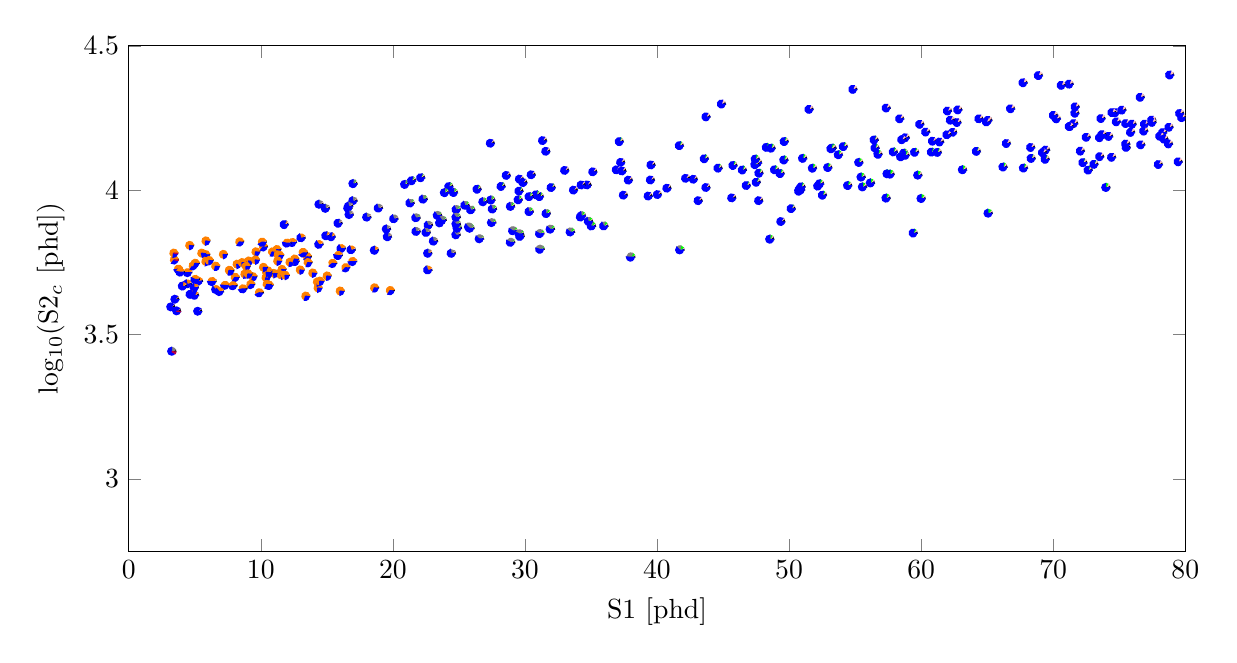
\begin{tikzpicture}
\centering
    \begin{axis}[
            ylabel={log${}_{10}$(S2$_c$ [phd])},
            xlabel={S1 [phd]},
            width=15cm,
            height=8cm,
            ymin=2.75, ymax=4.5,
            xmin=0, xmax=80,
            ]

\draw [black, fill=black] (40.00928,3.98382) -- (40.33150,3.98382) arc [start angle=0.00000,end angle=39.24027, radius=0.05cm] -- (40.00928,3.98382);
\draw [pink, fill=pink] (40.00928,3.98382) -- (40.25884,3.99322) arc [start angle=39.24027,end angle=57.94588, radius=0.05cm] -- (40.00928,3.98382);
\draw [blue, fill=blue] (40.00928,3.98382) -- (40.18029,3.99641) arc [start angle=57.94588,end angle=357.27905, radius=0.05cm] -- (40.00928,3.98382);

\draw [black, fill=black] (12.57129,3.75414) -- (12.89351,3.75414) arc [start angle=0.00000,end angle=10.90037, radius=0.05cm] -- (12.57129,3.75414);
\draw [orange, fill=orange] (12.57129,3.75414) -- (12.88769,3.75695) arc [start angle=10.90037,end angle=257.35718, radius=0.05cm] -- (12.57129,3.75414);
\draw [blue, fill=blue] (12.57129,3.75414) -- (12.50076,3.73964) arc [start angle=257.35718,end angle=356.30690, radius=0.05cm] -- (12.57129,3.75414);

\draw [black, fill=black] (7.28195,3.67028) -- (7.60417,3.67028) arc [start angle=0.00000,end angle=20.52712, radius=0.05cm] -- (7.28195,3.67028);
\draw [orange, fill=orange] (7.28195,3.67028) -- (7.58371,3.67549) arc [start angle=20.52712,end angle=175.25376, radius=0.05cm] -- (7.28195,3.67028);
\draw [blue, fill=blue] (7.28195,3.67028) -- (6.96083,3.67151) arc [start angle=175.25376,end angle=354.73875, radius=0.05cm] -- (7.28195,3.67028);

\draw [black, fill=black] (11.36268,3.71118) -- (11.68490,3.71118) arc [start angle=0.00000,end angle=9.34337, radius=0.05cm] -- (11.36268,3.71118);
\draw [orange, fill=orange] (11.36268,3.71118) -- (11.68063,3.71359) arc [start angle=9.34337,end angle=275.27157, radius=0.05cm] -- (11.36268,3.71118);
\draw [blue, fill=blue] (11.36268,3.71118) -- (11.39228,3.69638) arc [start angle=275.27157,end angle=357.27668, radius=0.05cm] -- (11.36268,3.71118);

\draw [black, fill=black] (62.36395,4.19937) -- (62.68617,4.19937) arc [start angle=0.00000,end angle=35.37095, radius=0.05cm] -- (62.36395,4.19937);
\draw [pink, fill=pink] (62.36395,4.19937) -- (62.62670,4.20797) arc [start angle=35.37095,end angle=63.32370, radius=0.05cm] -- (62.36395,4.19937);
\draw [blue, fill=blue] (62.36395,4.19937) -- (62.50861,4.21265) arc [start angle=63.32370,end angle=359.19930, radius=0.05cm] -- (62.36395,4.19937);

\draw [black, fill=black] (5.80901,3.77719) -- (6.13124,3.77719) arc [start angle=0.00000,end angle=9.11971, radius=0.05cm] -- (5.80901,3.77719);
\draw [orange, fill=orange] (5.80901,3.77719) -- (6.12716,3.77954) arc [start angle=9.11971,end angle=278.91012, radius=0.05cm] -- (5.80901,3.77719);
\draw [blue, fill=blue] (5.80901,3.77719) -- (5.85892,3.76251) arc [start angle=278.91012,end angle=356.87069, radius=0.05cm] -- (5.80901,3.77719);

\draw [black, fill=black] (53.23484,4.14475) -- (53.55706,4.14475) arc [start angle=0.00000,end angle=36.35484, radius=0.05cm] -- (53.23484,4.14475);
\draw [pink, fill=pink] (53.23484,4.14475) -- (53.49434,4.15356) arc [start angle=36.35484,end angle=59.32450, radius=0.05cm] -- (53.23484,4.14475);
\draw [green, fill=green] (53.23484,4.14475) -- (53.39923,4.15753) arc [start angle=59.32450,end angle=74.30965, radius=0.05cm] -- (53.23484,4.14475);
\draw [blue, fill=blue] (53.23484,4.14475) -- (53.32198,4.15906) arc [start angle=74.30965,end angle=359.99542, radius=0.05cm] -- (53.23484,4.14475);

\draw [black, fill=black] (3.74730,3.72675) -- (4.06952,3.72675) arc [start angle=0.00000,end angle=18.46297, radius=0.05cm] -- (3.74730,3.72675);
\draw [pink, fill=pink] (3.74730,3.72675) -- (4.05294,3.73145) arc [start angle=18.46297,end angle=23.52389, radius=0.05cm] -- (3.74730,3.72675);
\draw [orange, fill=orange] (3.74730,3.72675) -- (4.04274,3.73268) arc [start angle=23.52389,end angle=189.71431, radius=0.05cm] -- (3.74730,3.72675);
\draw [blue, fill=blue] (3.74730,3.72675) -- (3.42970,3.72424) arc [start angle=189.71431,end angle=355.38171, radius=0.05cm] -- (3.74730,3.72675);

\draw [black, fill=black] (59.98510,3.97001) -- (60.30732,3.97001) arc [start angle=0.00000,end angle=32.60080, radius=0.05cm] -- (59.98510,3.97001);
\draw [pink, fill=pink] (59.98510,3.97001) -- (60.25655,3.97802) arc [start angle=32.60080,end angle=52.78355, radius=0.05cm] -- (59.98510,3.97001);
\draw [green, fill=green] (59.98510,3.97001) -- (60.17998,3.98184) arc [start angle=52.78355,end angle=87.73142, radius=0.05cm] -- (59.98510,3.97001);
\draw [blue, fill=blue] (59.98510,3.97001) -- (59.99785,3.98486) arc [start angle=87.73142,end angle=359.93131, radius=0.05cm] -- (59.98510,3.97001);

\draw [black, fill=black] (27.40352,3.96478) -- (27.72574,3.96478) arc [start angle=0.00000,end angle=35.53417, radius=0.05cm] -- (27.40352,3.96478);
\draw [pink, fill=pink] (27.40352,3.96478) -- (27.66573,3.97342) arc [start angle=35.53417,end angle=49.80231, radius=0.05cm] -- (27.40352,3.96478);
\draw [green, fill=green] (27.40352,3.96478) -- (27.61149,3.97613) arc [start angle=49.80231,end angle=65.38089, radius=0.05cm] -- (27.40352,3.96478);
\draw [gray, fill=gray] (27.40352,3.96478) -- (27.53775,3.97829) arc [start angle=65.38089,end angle=88.38437, radius=0.05cm] -- (27.40352,3.96478);
\draw [blue, fill=blue] (27.40352,3.96478) -- (27.41260,3.97963) arc [start angle=88.38437,end angle=359.97263, radius=0.05cm] -- (27.40352,3.96478);

\draw [black, fill=black] (74.66848,4.26732) -- (74.99070,4.26732) arc [start angle=0.00000,end angle=35.15746, radius=0.05cm] -- (74.66848,4.26732);
\draw [pink, fill=pink] (74.66848,4.26732) -- (74.93192,4.27588) arc [start angle=35.15746,end angle=68.23490, radius=0.05cm] -- (74.66848,4.26732);
\draw [blue, fill=blue] (74.66848,4.26732) -- (74.78796,4.28112) arc [start angle=68.23490,end angle=359.99853, radius=0.05cm] -- (74.66848,4.26732);

\draw [black, fill=black] (78.26501,4.19843) -- (78.58724,4.19843) arc [start angle=0.00000,end angle=35.21454, radius=0.05cm] -- (78.26501,4.19843);
\draw [pink, fill=pink] (78.26501,4.19843) -- (78.52827,4.20700) arc [start angle=35.21454,end angle=66.47614, radius=0.05cm] -- (78.26501,4.19843);
\draw [blue, fill=blue] (78.26501,4.19843) -- (78.39362,4.21205) arc [start angle=66.47614,end angle=359.99228, radius=0.05cm] -- (78.26501,4.19843);

\draw [black, fill=black] (10.37297,3.69747) -- (10.69520,3.69747) arc [start angle=0.00000,end angle=10.46780, radius=0.05cm] -- (10.37297,3.69747);
\draw [orange, fill=orange] (10.37297,3.69747) -- (10.68983,3.70017) arc [start angle=10.46780,end angle=265.28389, radius=0.05cm] -- (10.37297,3.69747);
\draw [blue, fill=blue] (10.37297,3.69747) -- (10.34648,3.68266) arc [start angle=265.28389,end angle=356.95812, radius=0.05cm] -- (10.37297,3.69747);

\draw [black, fill=black] (25.88875,3.93087) -- (26.21097,3.93087) arc [start angle=0.00000,end angle=32.22008, radius=0.05cm] -- (25.88875,3.93087);
\draw [pink, fill=pink] (25.88875,3.93087) -- (26.16135,3.93879) arc [start angle=32.22008,end angle=44.67690, radius=0.05cm] -- (25.88875,3.93087);
\draw [green, fill=green] (25.88875,3.93087) -- (26.11788,3.94132) arc [start angle=44.67690,end angle=58.56452, radius=0.05cm] -- (25.88875,3.93087);
\draw [gray, fill=gray] (25.88875,3.93087) -- (26.05680,3.94355) arc [start angle=58.56452,end angle=115.55799, radius=0.05cm] -- (25.88875,3.93087);
\draw [blue, fill=blue] (25.88875,3.93087) -- (25.74974,3.94427) arc [start angle=115.55799,end angle=359.97050, radius=0.05cm] -- (25.88875,3.93087);

\draw [black, fill=black] (79.70562,4.25023) -- (80.02784,4.25023) arc [start angle=0.00000,end angle=35.59535, radius=0.05cm] -- (79.70562,4.25023);
\draw [pink, fill=pink] (79.70562,4.25023) -- (79.96763,4.25887) arc [start angle=35.59535,end angle=69.87197, radius=0.05cm] -- (79.70562,4.25023);
\draw [blue, fill=blue] (79.70562,4.25023) -- (79.81650,4.26418) arc [start angle=69.87197,end angle=359.99874, radius=0.05cm] -- (79.70562,4.25023);

\draw [black, fill=black] (25.73676,3.87174) -- (26.05899,3.87174) arc [start angle=0.00000,end angle=27.84138, radius=0.05cm] -- (25.73676,3.87174);
\draw [pink, fill=pink] (25.73676,3.87174) -- (26.02169,3.87868) arc [start angle=27.84138,end angle=38.31557, radius=0.05cm] -- (25.73676,3.87174);
\draw [green, fill=green] (25.73676,3.87174) -- (25.98958,3.88095) arc [start angle=38.31557,end angle=45.84109, radius=0.05cm] -- (25.73676,3.87174);
\draw [gray, fill=gray] (25.73676,3.87174) -- (25.96124,3.88240) arc [start angle=45.84109,end angle=136.13511, radius=0.05cm] -- (25.73676,3.87174);
\draw [blue, fill=blue] (25.73676,3.87174) -- (25.50445,3.88204) arc [start angle=136.13511,end angle=359.96069, radius=0.05cm] -- (25.73676,3.87174);

\draw [black, fill=black] (26.80824,3.95862) -- (27.13046,3.95862) arc [start angle=0.00000,end angle=34.55492, radius=0.05cm] -- (26.80824,3.95862);
\draw [pink, fill=pink] (26.80824,3.95862) -- (27.07362,3.96704) arc [start angle=34.55492,end angle=48.62502, radius=0.05cm] -- (26.80824,3.95862);
\draw [green, fill=green] (26.80824,3.95862) -- (27.02122,3.96976) arc [start angle=48.62502,end angle=63.99245, radius=0.05cm] -- (26.80824,3.95862);
\draw [gray, fill=gray] (26.80824,3.95862) -- (26.94953,3.97197) arc [start angle=63.99245,end angle=95.17134, radius=0.05cm] -- (26.80824,3.95862);
\draw [blue, fill=blue] (26.80824,3.95862) -- (26.77920,3.97341) arc [start angle=95.17134,end angle=359.97128, radius=0.05cm] -- (26.80824,3.95862);

\draw [black, fill=black] (9.06497,3.75501) -- (9.38720,3.75501) arc [start angle=0.00000,end angle=8.83622, radius=0.05cm] -- (9.06497,3.75501);
\draw [orange, fill=orange] (9.06497,3.75501) -- (9.38337,3.75729) arc [start angle=8.83622,end angle=280.04115, radius=0.05cm] -- (9.06497,3.75501);
\draw [blue, fill=blue] (9.06497,3.75501) -- (9.12115,3.74038) arc [start angle=280.04115,end angle=357.30339, radius=0.05cm] -- (9.06497,3.75501);

\draw [black, fill=black] (9.37781,3.70068) -- (9.70003,3.70068) arc [start angle=0.00000,end angle=11.29880, radius=0.05cm] -- (9.37781,3.70068);
\draw [orange, fill=orange] (9.37781,3.70068) -- (9.69378,3.70359) arc [start angle=11.29880,end angle=259.66173, radius=0.05cm] -- (9.37781,3.70068);
\draw [blue, fill=blue] (9.37781,3.70068) -- (9.31998,3.68606) arc [start angle=259.66173,end angle=356.81584, radius=0.05cm] -- (9.37781,3.70068);

\draw [black, fill=black] (57.32886,4.28360) -- (57.65108,4.28360) arc [start angle=0.00000,end angle=35.86768, radius=0.05cm] -- (57.32886,4.28360);
\draw [pink, fill=pink] (57.32886,4.28360) -- (57.58998,4.29231) arc [start angle=35.86768,end angle=66.71942, radius=0.05cm] -- (57.32886,4.28360);
\draw [blue, fill=blue] (57.32886,4.28360) -- (57.45621,4.29725) arc [start angle=66.71942,end angle=359.99174, radius=0.05cm] -- (57.32886,4.28360);

\draw [black, fill=black] (52.15371,4.01296) -- (52.47594,4.01296) arc [start angle=0.00000,end angle=36.77109, radius=0.05cm] -- (52.15371,4.01296);
\draw [pink, fill=pink] (52.15371,4.01296) -- (52.41182,4.02186) arc [start angle=36.77109,end angle=57.69711, radius=0.05cm] -- (52.15371,4.01296);
\draw [green, fill=green] (52.15371,4.01296) -- (52.32591,4.02552) arc [start angle=57.69711,end angle=76.66904, radius=0.05cm] -- (52.15371,4.01296);
\draw [blue, fill=blue] (52.15371,4.01296) -- (52.22801,4.02742) arc [start angle=76.66904,end angle=359.98561, radius=0.05cm] -- (52.15371,4.01296);

\draw [black, fill=black] (72.62480,4.06848) -- (72.94702,4.06848) arc [start angle=0.00000,end angle=35.73618, radius=0.05cm] -- (72.62480,4.06848);
\draw [pink, fill=pink] (72.62480,4.06848) -- (72.88635,4.07716) arc [start angle=35.73618,end angle=61.45395, radius=0.05cm] -- (72.62480,4.06848);
\draw [green, fill=green] (72.62480,4.06848) -- (72.77878,4.08153) arc [start angle=61.45395,end angle=73.28572, radius=0.05cm] -- (72.62480,4.06848);
\draw [blue, fill=blue] (72.62480,4.06848) -- (72.71747,4.08271) arc [start angle=73.28572,end angle=359.98488, radius=0.05cm] -- (72.62480,4.06848);

\draw [black, fill=black] (30.30806,3.92453) -- (30.63028,3.92453) arc [start angle=0.00000,end angle=33.76827, radius=0.05cm] -- (30.30806,3.92453);
\draw [pink, fill=pink] (30.30806,3.92453) -- (30.57592,3.93278) arc [start angle=33.76827,end angle=47.00413, radius=0.05cm] -- (30.30806,3.92453);
\draw [green, fill=green] (30.30806,3.92453) -- (30.52779,3.93539) arc [start angle=47.00413,end angle=66.33596, radius=0.05cm] -- (30.30806,3.92453);
\draw [gray, fill=gray] (30.30806,3.92453) -- (30.43739,3.93813) arc [start angle=66.33596,end angle=104.95340, radius=0.05cm] -- (30.30806,3.92453);
\draw [blue, fill=blue] (30.30806,3.92453) -- (30.22491,3.93888) arc [start angle=104.95340,end angle=359.97399, radius=0.05cm] -- (30.30806,3.92453);

\draw [black, fill=black] (56.48796,4.14503) -- (56.81018,4.14503) arc [start angle=0.00000,end angle=35.29636, radius=0.05cm] -- (56.48796,4.14503);
\draw [pink, fill=pink] (56.48796,4.14503) -- (56.75095,4.15362) arc [start angle=35.29636,end angle=60.04975, radius=0.05cm] -- (56.48796,4.14503);
\draw [green, fill=green] (56.48796,4.14503) -- (56.64883,4.15790) arc [start angle=60.04975,end angle=72.77544, radius=0.05cm] -- (56.48796,4.14503);
\draw [blue, fill=blue] (56.48796,4.14503) -- (56.58338,4.15922) arc [start angle=72.77544,end angle=359.99609, radius=0.05cm] -- (56.48796,4.14503);

\draw [black, fill=black] (14.30739,3.66165) -- (14.62961,3.66165) arc [start angle=0.00000,end angle=9.88354, radius=0.05cm] -- (14.30739,3.66165);
\draw [orange, fill=orange] (14.30739,3.66165) -- (14.62483,3.66420) arc [start angle=9.88354,end angle=270.92869, radius=0.05cm] -- (14.30739,3.66165);
\draw [blue, fill=blue] (14.30739,3.66165) -- (14.31261,3.64680) arc [start angle=270.92869,end angle=357.08275, radius=0.05cm] -- (14.30739,3.66165);

\draw [black, fill=black] (45.63678,3.97239) -- (45.95901,3.97239) arc [start angle=0.00000,end angle=37.04823, radius=0.05cm] -- (45.63678,3.97239);
\draw [pink, fill=pink] (45.63678,3.97239) -- (45.89396,3.98134) arc [start angle=37.04823,end angle=56.07428, radius=0.05cm] -- (45.63678,3.97239);
\draw [blue, fill=blue] (45.63678,3.97239) -- (45.81662,3.98472) arc [start angle=56.07428,end angle=356.92672, radius=0.05cm] -- (45.63678,3.97239);

\draw [black, fill=black] (14.39964,3.95009) -- (14.72186,3.95009) arc [start angle=0.00000,end angle=33.40257, radius=0.05cm] -- (14.39964,3.95009);
\draw [pink, fill=pink] (14.39964,3.95009) -- (14.66864,3.95827) arc [start angle=33.40257,end angle=45.45729, radius=0.05cm] -- (14.39964,3.95009);
\draw [gray, fill=gray] (14.39964,3.95009) -- (14.62566,3.96068) arc [start angle=45.45729,end angle=90.77698, radius=0.05cm] -- (14.39964,3.95009);
\draw [blue, fill=blue] (14.39964,3.95009) -- (14.39527,3.96495) arc [start angle=90.77698,end angle=357.87644, radius=0.05cm] -- (14.39964,3.95009);

\draw [black, fill=black] (24.41422,3.78011) -- (24.73644,3.78011) arc [start angle=0.00000,end angle=31.22533, radius=0.05cm] -- (24.41422,3.78011);
\draw [pink, fill=pink] (24.41422,3.78011) -- (24.68976,3.78782) arc [start angle=31.22533,end angle=42.51590, radius=0.05cm] -- (24.41422,3.78011);
\draw [gray, fill=gray] (24.41422,3.78011) -- (24.65173,3.79015) arc [start angle=42.51590,end angle=100.84322, radius=0.05cm] -- (24.41422,3.78011);
\draw [blue, fill=blue] (24.41422,3.78011) -- (24.35360,3.79471) arc [start angle=100.84322,end angle=356.29243, radius=0.05cm] -- (24.41422,3.78011);

\draw [black, fill=black] (11.19674,3.79452) -- (11.51897,3.79452) arc [start angle=0.00000,end angle=14.24280, radius=0.05cm] -- (11.19674,3.79452);
\draw [orange, fill=orange] (11.19674,3.79452) -- (11.50906,3.79818) arc [start angle=14.24280,end angle=230.19119, radius=0.05cm] -- (11.19674,3.79452);
\draw [blue, fill=blue] (11.19674,3.79452) -- (10.99045,3.78311) arc [start angle=230.19119,end angle=355.33112, radius=0.05cm] -- (11.19674,3.79452);

\draw [black, fill=black] (33.65458,3.99933) -- (33.97680,3.99933) arc [start angle=0.00000,end angle=38.35134, radius=0.05cm] -- (33.65458,3.99933);
\draw [pink, fill=pink] (33.65458,3.99933) -- (33.90727,4.00855) arc [start angle=38.35134,end angle=56.43238, radius=0.05cm] -- (33.65458,3.99933);
\draw [blue, fill=blue] (33.65458,3.99933) -- (33.83274,4.01171) arc [start angle=56.43238,end angle=353.99261, radius=0.05cm] -- (33.65458,3.99933);

\draw [black, fill=black] (13.91094,3.71338) -- (14.23316,3.71338) arc [start angle=0.00000,end angle=10.08942, radius=0.05cm] -- (13.91094,3.71338);
\draw [orange, fill=orange] (13.91094,3.71338) -- (14.22817,3.71598) arc [start angle=10.08942,end angle=268.79732, radius=0.05cm] -- (13.91094,3.71338);
\draw [blue, fill=blue] (13.91094,3.71338) -- (13.90417,3.69852) arc [start angle=268.79732,end angle=356.87104, radius=0.05cm] -- (13.91094,3.71338);

\draw [black, fill=black] (8.17713,3.74377) -- (8.49935,3.74377) arc [start angle=0.00000,end angle=9.46148, radius=0.05cm] -- (8.17713,3.74377);
\draw [orange, fill=orange] (8.17713,3.74377) -- (8.49496,3.74622) arc [start angle=9.46148,end angle=275.16549, radius=0.05cm] -- (8.17713,3.74377);
\draw [blue, fill=blue] (8.17713,3.74377) -- (8.20614,3.72898) arc [start angle=275.16549,end angle=357.21624, radius=0.05cm] -- (8.17713,3.74377);

\draw [black, fill=black] (36.89751,4.06951) -- (37.21973,4.06951) arc [start angle=0.00000,end angle=38.88888, radius=0.05cm] -- (36.89751,4.06951);
\draw [pink, fill=pink] (36.89751,4.06951) -- (37.14832,4.07884) arc [start angle=38.88888,end angle=58.32781, radius=0.05cm] -- (36.89751,4.06951);
\draw [blue, fill=blue] (36.89751,4.06951) -- (37.06670,4.08215) arc [start angle=58.32781,end angle=358.29037, radius=0.05cm] -- (36.89751,4.06951);

\draw [black, fill=black] (47.69737,4.05776) -- (48.01959,4.05776) arc [start angle=0.00000,end angle=37.79022, radius=0.05cm] -- (47.69737,4.05776);
\draw [pink, fill=pink] (47.69737,4.05776) -- (47.95201,4.06686) arc [start angle=37.79022,end angle=58.88347, radius=0.05cm] -- (47.69737,4.05776);
\draw [green, fill=green] (47.69737,4.05776) -- (47.86389,4.07048) arc [start angle=58.88347,end angle=73.60204, radius=0.05cm] -- (47.69737,4.05776);
\draw [blue, fill=blue] (47.69737,4.05776) -- (47.78833,4.07201) arc [start angle=73.60204,end angle=359.99194, radius=0.05cm] -- (47.69737,4.05776);

\draw [black, fill=black] (27.36173,4.16159) -- (27.68395,4.16159) arc [start angle=0.00000,end angle=39.15732, radius=0.05cm] -- (27.36173,4.16159);
\draw [pink, fill=pink] (27.36173,4.16159) -- (27.61158,4.17097) arc [start angle=39.15732,end angle=57.15222, radius=0.05cm] -- (27.36173,4.16159);
\draw [blue, fill=blue] (27.36173,4.16159) -- (27.53650,4.17407) arc [start angle=57.15222,end angle=359.06932, radius=0.05cm] -- (27.36173,4.16159);

\draw [black, fill=black] (38.00267,3.76806) -- (38.32489,3.76806) arc [start angle=0.00000,end angle=23.34068, radius=0.05cm] -- (38.00267,3.76806);
\draw [pink, fill=pink] (38.00267,3.76806) -- (38.29852,3.77395) arc [start angle=23.34068,end angle=32.22509, radius=0.05cm] -- (38.00267,3.76806);
\draw [green, fill=green] (38.00267,3.76806) -- (38.27526,3.77599) arc [start angle=32.22509,end angle=62.04172, radius=0.05cm] -- (38.00267,3.76806);
\draw [gray, fill=gray] (38.00267,3.76806) -- (38.15374,3.78119) arc [start angle=62.04172,end angle=176.67875, radius=0.05cm] -- (38.00267,3.76806);
\draw [blue, fill=blue] (38.00267,3.76806) -- (37.68099,3.76893) arc [start angle=176.67875,end angle=358.91552, radius=0.05cm] -- (38.00267,3.76806);

\draw [black, fill=black] (59.48688,4.13005) -- (59.80910,4.13005) arc [start angle=0.00000,end angle=36.07861, radius=0.05cm] -- (59.48688,4.13005);
\draw [pink, fill=pink] (59.48688,4.13005) -- (59.74730,4.13880) arc [start angle=36.07861,end angle=60.59168, radius=0.05cm] -- (59.48688,4.13005);
\draw [green, fill=green] (59.48688,4.13005) -- (59.64510,4.14299) arc [start angle=60.59168,end angle=73.56489, radius=0.05cm] -- (59.48688,4.13005);
\draw [blue, fill=blue] (59.48688,4.13005) -- (59.57804,4.14430) arc [start angle=73.56489,end angle=359.99593, radius=0.05cm] -- (59.48688,4.13005);

\draw [black, fill=black] (29.53017,3.99585) -- (29.85239,3.99585) arc [start angle=0.00000,end angle=37.73687, radius=0.05cm] -- (29.53017,3.99585);
\draw [pink, fill=pink] (29.53017,3.99585) -- (29.78499,4.00494) arc [start angle=37.73687,end angle=54.74631, radius=0.05cm] -- (29.53017,3.99585);
\draw [green, fill=green] (29.53017,3.99585) -- (29.71615,4.00798) arc [start angle=54.74631,end angle=63.91207, radius=0.05cm] -- (29.53017,3.99585);
\draw [blue, fill=blue] (29.53017,3.99585) -- (29.67187,4.00919) arc [start angle=63.91207,end angle=355.88105, radius=0.05cm] -- (29.53017,3.99585);

\draw [black, fill=black] (13.03509,3.83414) -- (13.35731,3.83414) arc [start angle=0.00000,end angle=27.53499, radius=0.05cm] -- (13.03509,3.83414);
\draw [pink, fill=pink] (13.03509,3.83414) -- (13.32082,3.84101) arc [start angle=27.53499,end angle=36.78957, radius=0.05cm] -- (13.03509,3.83414);
\draw [orange, fill=orange] (13.03509,3.83414) -- (13.29314,3.84304) arc [start angle=36.78957,end angle=108.53545, radius=0.05cm] -- (13.03509,3.83414);
\draw [blue, fill=blue] (13.03509,3.83414) -- (12.93266,3.84823) arc [start angle=108.53545,end angle=357.45637, radius=0.05cm] -- (13.03509,3.83414);

\draw [black, fill=black] (53.71547,4.12159) -- (54.03769,4.12159) arc [start angle=0.00000,end angle=35.67012, radius=0.05cm] -- (53.71547,4.12159);
\draw [pink, fill=pink] (53.71547,4.12159) -- (53.97724,4.13025) arc [start angle=35.67012,end angle=58.95723, radius=0.05cm] -- (53.71547,4.12159);
\draw [green, fill=green] (53.71547,4.12159) -- (53.88163,4.13432) arc [start angle=58.95723,end angle=80.23885, radius=0.05cm] -- (53.71547,4.12159);
\draw [blue, fill=blue] (53.71547,4.12159) -- (53.77010,4.13623) arc [start angle=80.23885,end angle=359.99504, radius=0.05cm] -- (53.71547,4.12159);

\draw [black, fill=black] (58.67392,4.12733) -- (58.99614,4.12733) arc [start angle=0.00000,end angle=35.91110, radius=0.05cm] -- (58.67392,4.12733);
\draw [pink, fill=pink] (58.67392,4.12733) -- (58.93490,4.13604) arc [start angle=35.91110,end angle=60.17064, radius=0.05cm] -- (58.67392,4.12733);
\draw [green, fill=green] (58.67392,4.12733) -- (58.83420,4.14022) arc [start angle=60.17064,end angle=74.94938, radius=0.05cm] -- (58.67392,4.12733);
\draw [blue, fill=blue] (58.67392,4.12733) -- (58.75759,4.14168) arc [start angle=74.94938,end angle=359.99574, radius=0.05cm] -- (58.67392,4.12733);

\draw [black, fill=black] (56.71368,4.12304) -- (57.03591,4.12304) arc [start angle=0.00000,end angle=35.12492, radius=0.05cm] -- (56.71368,4.12304);
\draw [pink, fill=pink] (56.71368,4.12304) -- (56.97723,4.13158) arc [start angle=35.12492,end angle=58.45088, radius=0.05cm] -- (56.71368,4.12304);
\draw [green, fill=green] (56.71368,4.12304) -- (56.88228,4.13570) arc [start angle=58.45088,end angle=77.44122, radius=0.05cm] -- (56.71368,4.12304);
\draw [blue, fill=blue] (56.71368,4.12304) -- (56.78375,4.13754) arc [start angle=77.44122,end angle=359.99562, radius=0.05cm] -- (56.71368,4.12304);

\draw [black, fill=black] (22.08357,4.04218) -- (22.40580,4.04218) arc [start angle=0.00000,end angle=38.30886, radius=0.05cm] -- (22.08357,4.04218);
\draw [pink, fill=pink] (22.08357,4.04218) -- (22.33642,4.05139) arc [start angle=38.30886,end angle=54.66832, radius=0.05cm] -- (22.08357,4.04218);
\draw [green, fill=green] (22.08357,4.04218) -- (22.26992,4.05430) arc [start angle=54.66832,end angle=61.88834, radius=0.05cm] -- (22.08357,4.04218);
\draw [gray, fill=gray] (22.08357,4.04218) -- (22.23540,4.05529) arc [start angle=61.88834,end angle=67.97837, radius=0.05cm] -- (22.08357,4.04218);
\draw [blue, fill=blue] (22.08357,4.04218) -- (22.20439,4.05596) arc [start angle=67.97837,end angle=359.84745, radius=0.05cm] -- (22.08357,4.04218);

\draw [black, fill=black] (9.87382,3.64493) -- (10.19604,3.64493) arc [start angle=0.00000,end angle=16.91809, radius=0.05cm] -- (9.87382,3.64493);
\draw [orange, fill=orange] (9.87382,3.64493) -- (10.18209,3.64925) arc [start angle=16.91809,end angle=207.44135, radius=0.05cm] -- (9.87382,3.64493);
\draw [blue, fill=blue] (9.87382,3.64493) -- (9.58785,3.63808) arc [start angle=207.44135,end angle=355.24265, radius=0.05cm] -- (9.87382,3.64493);

\draw [black, fill=black] (6.59143,3.65534) -- (6.91366,3.65534) arc [start angle=0.00000,end angle=26.13297, radius=0.05cm] -- (6.59143,3.65534);
\draw [pink, fill=pink] (6.59143,3.65534) -- (6.88072,3.66188) arc [start angle=26.13297,end angle=32.37046, radius=0.05cm] -- (6.59143,3.65534);
\draw [orange, fill=orange] (6.59143,3.65534) -- (6.86358,3.66329) arc [start angle=32.37046,end angle=133.15427, radius=0.05cm] -- (6.59143,3.65534);
\draw [blue, fill=blue] (6.59143,3.65534) -- (6.37104,3.66618) arc [start angle=133.15427,end angle=359.17986, radius=0.05cm] -- (6.59143,3.65534);

\draw [black, fill=black] (57.40655,4.05558) -- (57.72877,4.05558) arc [start angle=0.00000,end angle=34.38003, radius=0.05cm] -- (57.40655,4.05558);
\draw [pink, fill=pink] (57.40655,4.05558) -- (57.67248,4.06397) arc [start angle=34.38003,end angle=55.73599, radius=0.05cm] -- (57.40655,4.05558);
\draw [green, fill=green] (57.40655,4.05558) -- (57.58796,4.06786) arc [start angle=55.73599,end angle=87.37920, radius=0.05cm] -- (57.40655,4.05558);
\draw [blue, fill=blue] (57.40655,4.05558) -- (57.42129,4.07042) arc [start angle=87.37920,end angle=359.99179, radius=0.05cm] -- (57.40655,4.05558);

\draw [black, fill=black] (9.21492,3.67386) -- (9.53714,3.67386) arc [start angle=0.00000,end angle=14.42225, radius=0.05cm] -- (9.21492,3.67386);
\draw [orange, fill=orange] (9.21492,3.67386) -- (9.52699,3.67756) arc [start angle=14.42225,end angle=230.33400, radius=0.05cm] -- (9.21492,3.67386);
\draw [blue, fill=blue] (9.21492,3.67386) -- (9.00924,3.66242) arc [start angle=230.33400,end angle=355.89140, radius=0.05cm] -- (9.21492,3.67386);

\draw [black, fill=black] (11.58248,3.72569) -- (11.90470,3.72569) arc [start angle=0.00000,end angle=9.10591, radius=0.05cm] -- (11.58248,3.72569);
\draw [orange, fill=orange] (11.58248,3.72569) -- (11.90064,3.72804) arc [start angle=9.10591,end angle=276.89355, radius=0.05cm] -- (11.58248,3.72569);
\draw [blue, fill=blue] (11.58248,3.72569) -- (11.62115,3.71094) arc [start angle=276.89355,end angle=357.32541, radius=0.05cm] -- (11.58248,3.72569);

\draw [black, fill=black] (4.46028,3.71452) -- (4.78250,3.71452) arc [start angle=0.00000,end angle=19.63519, radius=0.05cm] -- (4.46028,3.71452);
\draw [pink, fill=pink] (4.46028,3.71452) -- (4.76376,3.71952) arc [start angle=19.63519,end angle=24.78508, radius=0.05cm] -- (4.46028,3.71452);
\draw [orange, fill=orange] (4.46028,3.71452) -- (4.75282,3.72075) arc [start angle=24.78508,end angle=182.37259, radius=0.05cm] -- (4.46028,3.71452);
\draw [blue, fill=blue] (4.46028,3.71452) -- (4.13833,3.71391) arc [start angle=182.37259,end angle=358.02690, radius=0.05cm] -- (4.46028,3.71452);

\draw [black, fill=black] (8.76765,3.70998) -- (9.08987,3.70998) arc [start angle=0.00000,end angle=11.01540, radius=0.05cm] -- (8.76765,3.70998);
\draw [orange, fill=orange] (8.76765,3.70998) -- (9.08394,3.71282) arc [start angle=11.01540,end angle=260.42991, radius=0.05cm] -- (8.76765,3.70998);
\draw [blue, fill=blue] (8.76765,3.70998) -- (8.71408,3.69533) arc [start angle=260.42991,end angle=356.79437, radius=0.05cm] -- (8.76765,3.70998);

\draw [black, fill=black] (10.97286,3.71182) -- (11.29509,3.71182) arc [start angle=0.00000,end angle=9.40940, radius=0.05cm] -- (10.97286,3.71182);
\draw [orange, fill=orange] (10.97286,3.71182) -- (11.29075,3.71425) arc [start angle=9.40940,end angle=273.99308, radius=0.05cm] -- (10.97286,3.71182);
\draw [blue, fill=blue] (10.97286,3.71182) -- (10.99530,3.69700) arc [start angle=273.99308,end angle=357.22229, radius=0.05cm] -- (10.97286,3.71182);

\draw [black, fill=black] (8.03131,3.69842) -- (8.35353,3.69842) arc [start angle=0.00000,end angle=13.49889, radius=0.05cm] -- (8.03131,3.69842);
\draw [orange, fill=orange] (8.03131,3.69842) -- (8.34463,3.70189) arc [start angle=13.49889,end angle=238.26803, radius=0.05cm] -- (8.03131,3.69842);
\draw [blue, fill=blue] (8.03131,3.69842) -- (7.86184,3.68579) arc [start angle=238.26803,end angle=356.07376, radius=0.05cm] -- (8.03131,3.69842);

\draw [black, fill=black] (7.88370,3.66925) -- (8.20592,3.66925) arc [start angle=0.00000,end angle=18.84544, radius=0.05cm] -- (7.88370,3.66925);
\draw [orange, fill=orange] (7.88370,3.66925) -- (8.18864,3.67405) arc [start angle=18.84544,end angle=189.83197, radius=0.05cm] -- (7.88370,3.66925);
\draw [blue, fill=blue] (7.88370,3.66925) -- (7.56621,3.66672) arc [start angle=189.83197,end angle=355.06417, radius=0.05cm] -- (7.88370,3.66925);

\draw [black, fill=black] (10.85406,3.78625) -- (11.17628,3.78625) arc [start angle=0.00000,end angle=12.57515, radius=0.05cm] -- (10.85406,3.78625);
\draw [orange, fill=orange] (10.85406,3.78625) -- (11.16855,3.78949) arc [start angle=12.57515,end angle=246.09901, radius=0.05cm] -- (10.85406,3.78625);
\draw [blue, fill=blue] (10.85406,3.78625) -- (10.72351,3.77267) arc [start angle=246.09901,end angle=356.01970, radius=0.05cm] -- (10.85406,3.78625);

\draw [black, fill=black] (24.21967,4.01133) -- (24.54189,4.01133) arc [start angle=0.00000,end angle=37.17218, radius=0.05cm] -- (24.21967,4.01133);
\draw [pink, fill=pink] (24.21967,4.01133) -- (24.47642,4.02031) arc [start angle=37.17218,end angle=52.66992, radius=0.05cm] -- (24.21967,4.01133);
\draw [green, fill=green] (24.21967,4.01133) -- (24.41507,4.02314) arc [start angle=52.66992,end angle=63.80098, radius=0.05cm] -- (24.21967,4.01133);
\draw [gray, fill=gray] (24.21967,4.01133) -- (24.36193,4.02466) arc [start angle=63.80098,end angle=75.71657, radius=0.05cm] -- (24.21967,4.01133);
\draw [blue, fill=blue] (24.21967,4.01133) -- (24.29917,4.02573) arc [start angle=75.71657,end angle=359.93982, radius=0.05cm] -- (24.21967,4.01133);

\draw [black, fill=black] (47.49152,4.02644) -- (47.81374,4.02644) arc [start angle=0.00000,end angle=36.64019, radius=0.05cm] -- (47.49152,4.02644);
\draw [pink, fill=pink] (47.49152,4.02644) -- (47.75007,4.03531) arc [start angle=36.64019,end angle=57.01917, radius=0.05cm] -- (47.49152,4.02644);
\draw [green, fill=green] (47.49152,4.02644) -- (47.66692,4.03890) arc [start angle=57.01917,end angle=66.19605, radius=0.05cm] -- (47.49152,4.02644);
\draw [blue, fill=blue] (47.49152,4.02644) -- (47.62157,4.04004) arc [start angle=66.19605,end angle=359.98748, radius=0.05cm] -- (47.49152,4.02644);

\draw [black, fill=black] (13.18465,3.78420) -- (13.50687,3.78420) arc [start angle=0.00000,end angle=16.89647, radius=0.05cm] -- (13.18465,3.78420);
\draw [pink, fill=pink] (13.18465,3.78420) -- (13.49296,3.78852) arc [start angle=16.89647,end angle=22.30110, radius=0.05cm] -- (13.18465,3.78420);
\draw [orange, fill=orange] (13.18465,3.78420) -- (13.48277,3.78984) arc [start angle=22.30110,end angle=210.72307, radius=0.05cm] -- (13.18465,3.78420);
\draw [blue, fill=blue] (13.18465,3.78420) -- (12.90765,3.77661) arc [start angle=210.72307,end angle=359.63208, radius=0.05cm] -- (13.18465,3.78420);

\draw [black, fill=black] (71.61829,4.26542) -- (71.94051,4.26542) arc [start angle=0.00000,end angle=36.14616, radius=0.05cm] -- (71.61829,4.26542);
\draw [pink, fill=pink] (71.61829,4.26542) -- (71.87849,4.27418) arc [start angle=36.14616,end angle=69.01468, radius=0.05cm] -- (71.61829,4.26542);
\draw [blue, fill=blue] (71.61829,4.26542) -- (71.73368,4.27929) arc [start angle=69.01468,end angle=359.99827, radius=0.05cm] -- (71.61829,4.26542);

\draw [black, fill=black] (3.43062,3.75886) -- (3.75285,3.75886) arc [start angle=0.00000,end angle=12.77518, radius=0.05cm] -- (3.43062,3.75886);
\draw [orange, fill=orange] (3.43062,3.75886) -- (3.74487,3.76215) arc [start angle=12.77518,end angle=233.86793, radius=0.05cm] -- (3.43062,3.75886);
\draw [blue, fill=blue] (3.43062,3.75886) -- (3.24063,3.74686) arc [start angle=233.86793,end angle=349.85459, radius=0.05cm] -- (3.43062,3.75886);
\draw [purple, fill=purple] (3.43062,3.75886) -- (3.74781,3.75624) arc [start angle=349.85459,end angle=356.73763, radius=0.05cm] -- (3.43062,3.75886);

\draw [black, fill=black] (78.04781,4.18581) -- (78.37004,4.18581) arc [start angle=0.00000,end angle=35.78618, radius=0.05cm] -- (78.04781,4.18581);
\draw [pink, fill=pink] (78.04781,4.18581) -- (78.30920,4.19449) arc [start angle=35.78618,end angle=66.15768, radius=0.05cm] -- (78.04781,4.18581);
\draw [blue, fill=blue] (78.04781,4.18581) -- (78.17806,4.19940) arc [start angle=66.15768,end angle=359.97922, radius=0.05cm] -- (78.04781,4.18581);

\draw [black, fill=black] (75.50079,4.14713) -- (75.82302,4.14713) arc [start angle=0.00000,end angle=35.48602, radius=0.05cm] -- (75.50079,4.14713);
\draw [pink, fill=pink] (75.50079,4.14713) -- (75.76317,4.15575) arc [start angle=35.48602,end angle=64.03563, radius=0.05cm] -- (75.50079,4.14713);
\draw [blue, fill=blue] (75.50079,4.14713) -- (75.64187,4.16049) arc [start angle=64.03563,end angle=359.66558, radius=0.05cm] -- (75.50079,4.14713);

\draw [black, fill=black] (13.50055,3.76973) -- (13.82277,3.76973) arc [start angle=0.00000,end angle=14.54819, radius=0.05cm] -- (13.50055,3.76973);
\draw [orange, fill=orange] (13.50055,3.76973) -- (13.81244,3.77346) arc [start angle=14.54819,end angle=224.17330, radius=0.05cm] -- (13.50055,3.76973);
\draw [blue, fill=blue] (13.50055,3.76973) -- (13.26944,3.75937) arc [start angle=224.17330,end angle=354.95742, radius=0.05cm] -- (13.50055,3.76973);

\draw [black, fill=black] (13.21194,3.78294) -- (13.53416,3.78294) arc [start angle=0.00000,end angle=16.65484, radius=0.05cm] -- (13.21194,3.78294);
\draw [pink, fill=pink] (13.21194,3.78294) -- (13.52064,3.78720) arc [start angle=16.65484,end angle=22.00008, radius=0.05cm] -- (13.21194,3.78294);
\draw [orange, fill=orange] (13.21194,3.78294) -- (13.51069,3.78851) arc [start angle=22.00008,end angle=212.47722, radius=0.05cm] -- (13.21194,3.78294);
\draw [blue, fill=blue] (13.21194,3.78294) -- (12.94011,3.77496) arc [start angle=212.47722,end angle=359.63995, radius=0.05cm] -- (13.21194,3.78294);

\draw [black, fill=black] (69.39980,4.13815) -- (69.72203,4.13815) arc [start angle=0.00000,end angle=36.17046, radius=0.05cm] -- (69.39980,4.13815);
\draw [pink, fill=pink] (69.39980,4.13815) -- (69.65992,4.14692) arc [start angle=36.17046,end angle=64.54159, radius=0.05cm] -- (69.39980,4.13815);
\draw [blue, fill=blue] (69.39980,4.13815) -- (69.53831,4.15157) arc [start angle=64.54159,end angle=357.47883, radius=0.05cm] -- (69.39980,4.13815);

\draw [black, fill=black] (25.82528,3.86727) -- (26.14751,3.86727) arc [start angle=0.00000,end angle=27.66776, radius=0.05cm] -- (25.82528,3.86727);
\draw [pink, fill=pink] (25.82528,3.86727) -- (26.11066,3.87417) arc [start angle=27.66776,end angle=38.14299, radius=0.05cm] -- (25.82528,3.86727);
\draw [green, fill=green] (25.82528,3.86727) -- (26.07870,3.87644) arc [start angle=38.14299,end angle=45.59761, radius=0.05cm] -- (25.82528,3.86727);
\draw [gray, fill=gray] (25.82528,3.86727) -- (26.05074,3.87788) arc [start angle=45.59761,end angle=136.46083, radius=0.05cm] -- (25.82528,3.86727);
\draw [blue, fill=blue] (25.82528,3.86727) -- (25.59170,3.87750) arc [start angle=136.46083,end angle=359.95729, radius=0.05cm] -- (25.82528,3.86727);

\draw [black, fill=black] (50.85365,4.00018) -- (51.17588,4.00018) arc [start angle=0.00000,end angle=37.86635, radius=0.05cm] -- (50.85365,4.00018);
\draw [pink, fill=pink] (50.85365,4.00018) -- (51.10803,4.00930) arc [start angle=37.86635,end angle=58.16280, radius=0.05cm] -- (50.85365,4.00018);
\draw [green, fill=green] (50.85365,4.00018) -- (51.02363,4.01281) arc [start angle=58.16280,end angle=71.10395, radius=0.05cm] -- (50.85365,4.00018);
\draw [blue, fill=blue] (50.85365,4.00018) -- (50.95801,4.01424) arc [start angle=71.10395,end angle=359.98313, radius=0.05cm] -- (50.85365,4.00018);

\draw [black, fill=black] (43.68982,4.25296) -- (44.01204,4.25296) arc [start angle=0.00000,end angle=35.56481, radius=0.05cm] -- (43.68982,4.25296);
\draw [pink, fill=pink] (43.68982,4.25296) -- (43.95193,4.26160) arc [start angle=35.56481,end angle=62.39209, radius=0.05cm] -- (43.68982,4.25296);
\draw [blue, fill=blue] (43.68982,4.25296) -- (43.83914,4.26613) arc [start angle=62.39209,end angle=357.28483, radius=0.05cm] -- (43.68982,4.25296);

\draw [black, fill=black] (12.96318,3.72398) -- (13.28540,3.72398) arc [start angle=0.00000,end angle=9.76092, radius=0.05cm] -- (12.96318,3.72398);
\draw [orange, fill=orange] (12.96318,3.72398) -- (13.28074,3.72650) arc [start angle=9.76092,end angle=272.33896, radius=0.05cm] -- (12.96318,3.72398);
\draw [blue, fill=blue] (12.96318,3.72398) -- (12.97633,3.70914) arc [start angle=272.33896,end angle=357.07024, radius=0.05cm] -- (12.96318,3.72398);

\draw [black, fill=black] (30.45135,4.05244) -- (30.77357,4.05244) arc [start angle=0.00000,end angle=38.27187, radius=0.05cm] -- (30.45135,4.05244);
\draw [pink, fill=pink] (30.45135,4.05244) -- (30.70432,4.06164) arc [start angle=38.27187,end angle=55.95601, radius=0.05cm] -- (30.45135,4.05244);
\draw [blue, fill=blue] (30.45135,4.05244) -- (30.63174,4.06475) arc [start angle=55.95601,end angle=358.28228, radius=0.05cm] -- (30.45135,4.05244);

\draw [black, fill=black] (34.19564,3.90576) -- (34.51786,3.90576) arc [start angle=0.00000,end angle=33.48270, radius=0.05cm] -- (34.19564,3.90576);
\draw [pink, fill=pink] (34.19564,3.90576) -- (34.46439,3.91396) arc [start angle=33.48270,end angle=47.29402, radius=0.05cm] -- (34.19564,3.90576);
\draw [green, fill=green] (34.19564,3.90576) -- (34.41418,3.91668) arc [start angle=47.29402,end angle=70.22418, radius=0.05cm] -- (34.19564,3.90576);
\draw [gray, fill=gray] (34.19564,3.90576) -- (34.30466,3.91974) arc [start angle=70.22418,end angle=101.19197, radius=0.05cm] -- (34.19564,3.90576);
\draw [blue, fill=blue] (34.19564,3.90576) -- (34.13310,3.92034) arc [start angle=101.19197,end angle=359.96623, radius=0.05cm] -- (34.19564,3.90576);

\draw [black, fill=black] (9.60578,3.78682) -- (9.92800,3.78682) arc [start angle=0.00000,end angle=10.82698, radius=0.05cm] -- (9.60578,3.78682);
\draw [orange, fill=orange] (9.60578,3.78682) -- (9.92227,3.78961) arc [start angle=10.82698,end angle=261.92899, radius=0.05cm] -- (9.60578,3.78682);
\draw [blue, fill=blue] (9.60578,3.78682) -- (9.56054,3.77211) arc [start angle=261.92899,end angle=356.58907, radius=0.05cm] -- (9.60578,3.78682);

\draw [black, fill=black] (24.79088,3.93187) -- (25.11310,3.93187) arc [start angle=0.00000,end angle=31.10035, radius=0.05cm] -- (24.79088,3.93187);
\draw [pink, fill=pink] (24.79088,3.93187) -- (25.06678,3.93954) arc [start angle=31.10035,end angle=43.67080, radius=0.05cm] -- (24.79088,3.93187);
\draw [green, fill=green] (24.79088,3.93187) -- (25.02395,3.94213) arc [start angle=43.67080,end angle=55.80102, radius=0.05cm] -- (24.79088,3.93187);
\draw [gray, fill=gray] (24.79088,3.93187) -- (24.97199,3.94416) arc [start angle=55.80102,end angle=116.52039, radius=0.05cm] -- (24.79088,3.93187);
\draw [blue, fill=blue] (24.79088,3.93187) -- (24.64700,3.94516) arc [start angle=116.52039,end angle=359.96785, radius=0.05cm] -- (24.79088,3.93187);

\draw [black, fill=black] (12.38238,3.81852) -- (12.70460,3.81852) arc [start angle=0.00000,end angle=22.60363, radius=0.05cm] -- (12.38238,3.81852);
\draw [pink, fill=pink] (12.38238,3.81852) -- (12.67985,3.82423) arc [start angle=22.60363,end angle=30.22201, radius=0.05cm] -- (12.38238,3.81852);
\draw [orange, fill=orange] (12.38238,3.81852) -- (12.66080,3.82600) arc [start angle=30.22201,end angle=154.62677, radius=0.05cm] -- (12.38238,3.81852);
\draw [blue, fill=blue] (12.38238,3.81852) -- (12.09124,3.82489) arc [start angle=154.62677,end angle=359.04513, radius=0.05cm] -- (12.38238,3.81852);

\draw [black, fill=black] (31.91897,3.86417) -- (32.24119,3.86417) arc [start angle=0.00000,end angle=28.26439, radius=0.05cm] -- (31.91897,3.86417);
\draw [pink, fill=pink] (31.91897,3.86417) -- (32.20277,3.87120) arc [start angle=28.26439,end angle=39.42826, radius=0.05cm] -- (31.91897,3.86417);
\draw [green, fill=green] (31.91897,3.86417) -- (32.16786,3.87360) arc [start angle=39.42826,end angle=59.57254, radius=0.05cm] -- (31.91897,3.86417);
\draw [gray, fill=gray] (31.91897,3.86417) -- (32.08216,3.87698) arc [start angle=59.57254,end angle=138.27138, radius=0.05cm] -- (31.91897,3.86417);
\draw [blue, fill=blue] (31.91897,3.86417) -- (31.67849,3.87405) arc [start angle=138.27138,end angle=359.94971, radius=0.05cm] -- (31.91897,3.86417);

\draw [black, fill=black] (34.68143,4.01726) -- (35.00366,4.01726) arc [start angle=0.00000,end angle=38.88602, radius=0.05cm] -- (34.68143,4.01726);
\draw [pink, fill=pink] (34.68143,4.01726) -- (34.93225,4.02659) arc [start angle=38.88602,end angle=57.48592, radius=0.05cm] -- (34.68143,4.01726);
\draw [blue, fill=blue] (34.68143,4.01726) -- (34.85463,4.02979) arc [start angle=57.48592,end angle=357.65038, radius=0.05cm] -- (34.68143,4.01726);

\draw [black, fill=black] (19.78254,3.65262) -- (20.10476,3.65262) arc [start angle=0.00000,end angle=13.43477, radius=0.05cm] -- (19.78254,3.65262);
\draw [orange, fill=orange] (19.78254,3.65262) -- (20.09594,3.65608) arc [start angle=13.43477,end angle=239.11892, radius=0.05cm] -- (19.78254,3.65262);
\draw [blue, fill=blue] (19.78254,3.65262) -- (19.61716,3.63987) arc [start angle=239.11892,end angle=354.40440, radius=0.05cm] -- (19.78254,3.65262);

\draw [black, fill=black] (51.75199,4.07493) -- (52.07421,4.07493) arc [start angle=0.00000,end angle=35.91475, radius=0.05cm] -- (51.75199,4.07493);
\draw [pink, fill=pink] (51.75199,4.07493) -- (52.01296,4.08365) arc [start angle=35.91475,end angle=57.00316, radius=0.05cm] -- (51.75199,4.07493);
\draw [green, fill=green] (51.75199,4.07493) -- (51.92747,4.08740) arc [start angle=57.00316,end angle=81.36870, radius=0.05cm] -- (51.75199,4.07493);
\draw [blue, fill=blue] (51.75199,4.07493) -- (51.80035,4.08962) arc [start angle=81.36870,end angle=359.99303, radius=0.05cm] -- (51.75199,4.07493);

\draw [black, fill=black] (48.88320,4.06956) -- (49.20542,4.06956) arc [start angle=0.00000,end angle=36.44083, radius=0.05cm] -- (48.88320,4.06956);
\draw [pink, fill=pink] (48.88320,4.06956) -- (49.14242,4.07838) arc [start angle=36.44083,end angle=57.67390, radius=0.05cm] -- (48.88320,4.06956);
\draw [green, fill=green] (48.88320,4.06956) -- (49.05550,4.08211) arc [start angle=57.67390,end angle=75.88387, radius=0.05cm] -- (48.88320,4.06956);
\draw [blue, fill=blue] (48.88320,4.06956) -- (48.96178,4.08397) arc [start angle=75.88387,end angle=359.99251, radius=0.05cm] -- (48.88320,4.06956);

\draw [black, fill=black] (43.56231,4.10769) -- (43.88454,4.10769) arc [start angle=0.00000,end angle=37.15605, radius=0.05cm] -- (43.56231,4.10769);
\draw [pink, fill=pink] (43.56231,4.10769) -- (43.81912,4.11666) arc [start angle=37.15605,end angle=58.94890, radius=0.05cm] -- (43.56231,4.10769);
\draw [green, fill=green] (43.56231,4.10769) -- (43.72852,4.12041) arc [start angle=58.94890,end angle=71.42065, radius=0.05cm] -- (43.56231,4.10769);
\draw [blue, fill=blue] (43.56231,4.10769) -- (43.66498,4.12177) arc [start angle=71.42065,end angle=359.99113, radius=0.05cm] -- (43.56231,4.10769);

\draw [black, fill=black] (14.39428,3.81138) -- (14.71650,3.81138) arc [start angle=0.00000,end angle=27.16785, radius=0.05cm] -- (14.39428,3.81138);
\draw [pink, fill=pink] (14.39428,3.81138) -- (14.68095,3.81816) arc [start angle=27.16785,end angle=36.61744, radius=0.05cm] -- (14.39428,3.81138);
\draw [orange, fill=orange] (14.39428,3.81138) -- (14.65291,3.82024) arc [start angle=36.61744,end angle=123.10470, radius=0.05cm] -- (14.39428,3.81138);
\draw [blue, fill=blue] (14.39428,3.81138) -- (14.21829,3.82382) arc [start angle=123.10470,end angle=357.78757, radius=0.05cm] -- (14.39428,3.81138);

\draw [black, fill=black] (52.50610,3.98160) -- (52.82833,3.98160) arc [start angle=0.00000,end angle=36.50310, radius=0.05cm] -- (52.50610,3.98160);
\draw [pink, fill=pink] (52.50610,3.98160) -- (52.76511,3.99043) arc [start angle=36.50310,end angle=57.19954, radius=0.05cm] -- (52.50610,3.98160);
\draw [green, fill=green] (52.50610,3.98160) -- (52.68066,3.99408) arc [start angle=57.19954,end angle=71.54161, radius=0.05cm] -- (52.50610,3.98160);
\draw [blue, fill=blue] (52.50610,3.98160) -- (52.60812,3.99569) arc [start angle=71.54161,end angle=359.97542, radius=0.05cm] -- (52.50610,3.98160);

\draw [black, fill=black] (76.57004,4.32069) -- (76.89226,4.32069) arc [start angle=0.00000,end angle=35.14723, radius=0.05cm] -- (76.57004,4.32069);
\draw [pink, fill=pink] (76.57004,4.32069) -- (76.83351,4.32925) arc [start angle=35.14723,end angle=70.21783, radius=0.05cm] -- (76.57004,4.32069);
\draw [blue, fill=blue] (76.57004,4.32069) -- (76.67909,4.33468) arc [start angle=70.21783,end angle=359.99838, radius=0.05cm] -- (76.57004,4.32069);

\draw [black, fill=black] (11.28932,3.77616) -- (11.61154,3.77616) arc [start angle=0.00000,end angle=11.98598, radius=0.05cm] -- (11.28932,3.77616);
\draw [orange, fill=orange] (11.28932,3.77616) -- (11.60451,3.77925) arc [start angle=11.98598,end angle=250.98232, radius=0.05cm] -- (11.28932,3.77616);
\draw [blue, fill=blue] (11.28932,3.77616) -- (11.18432,3.76212) arc [start angle=250.98232,end angle=356.17297, radius=0.05cm] -- (11.28932,3.77616);

\draw [black, fill=black] (5.20191,3.58004) -- (5.52413,3.58004) arc [start angle=0.00000,end angle=34.72148, radius=0.05cm] -- (5.20191,3.58004);
\draw [pink, fill=pink] (5.20191,3.58004) -- (5.46675,3.58851) arc [start angle=34.72148,end angle=42.16626, radius=0.05cm] -- (5.20191,3.58004);
\draw [blue, fill=blue] (5.20191,3.58004) -- (5.44074,3.59002) arc [start angle=42.16626,end angle=352.12459, radius=0.05cm] -- (5.20191,3.58004);

\draw [black, fill=black] (16.58037,3.93697) -- (16.90259,3.93697) arc [start angle=0.00000,end angle=31.84759, radius=0.05cm] -- (16.58037,3.93697);
\draw [pink, fill=pink] (16.58037,3.93697) -- (16.85408,3.94481) arc [start angle=31.84759,end angle=42.58267, radius=0.05cm] -- (16.58037,3.93697);
\draw [gray, fill=gray] (16.58037,3.93697) -- (16.81762,3.94702) arc [start angle=42.58267,end angle=97.51798, radius=0.05cm] -- (16.58037,3.93697);
\draw [blue, fill=blue] (16.58037,3.93697) -- (16.53821,3.95170) arc [start angle=97.51798,end angle=357.51134, radius=0.05cm] -- (16.58037,3.93697);

\draw [black, fill=black] (8.56398,3.74955) -- (8.88621,3.74955) arc [start angle=0.00000,end angle=9.09555, radius=0.05cm] -- (8.56398,3.74955);
\draw [orange, fill=orange] (8.56398,3.74955) -- (8.88216,3.75190) arc [start angle=9.09555,end angle=278.95102, radius=0.05cm] -- (8.56398,3.74955);
\draw [blue, fill=blue] (8.56398,3.74955) -- (8.61412,3.73487) arc [start angle=278.95102,end angle=357.31877, radius=0.05cm] -- (8.56398,3.74955);

\draw [black, fill=black] (41.67576,4.15322) -- (41.99798,4.15322) arc [start angle=0.00000,end angle=37.17516, radius=0.05cm] -- (41.67576,4.15322);
\draw [pink, fill=pink] (41.67576,4.15322) -- (41.93250,4.16220) arc [start angle=37.17516,end angle=60.03971, radius=0.05cm] -- (41.67576,4.15322);
\draw [green, fill=green] (41.67576,4.15322) -- (41.83668,4.16609) arc [start angle=60.03971,end angle=73.42424, radius=0.05cm] -- (41.67576,4.15322);
\draw [blue, fill=blue] (41.67576,4.15322) -- (41.76768,4.16746) arc [start angle=73.42424,end angle=359.98597, radius=0.05cm] -- (41.67576,4.15322);

\draw [black, fill=black] (58.77532,4.18080) -- (59.09754,4.18080) arc [start angle=0.00000,end angle=37.03897, radius=0.05cm] -- (58.77532,4.18080);
\draw [pink, fill=pink] (58.77532,4.18080) -- (59.03252,4.18975) arc [start angle=37.03897,end angle=63.69583, radius=0.05cm] -- (58.77532,4.18080);
\draw [blue, fill=blue] (58.77532,4.18080) -- (58.91811,4.19412) arc [start angle=63.69583,end angle=356.92800, radius=0.05cm] -- (58.77532,4.18080);

\draw [black, fill=black] (60.75870,4.13075) -- (61.08092,4.13075) arc [start angle=0.00000,end angle=35.85189, radius=0.05cm] -- (60.75870,4.13075);
\draw [pink, fill=pink] (60.75870,4.13075) -- (61.01987,4.13946) arc [start angle=35.85189,end angle=61.34264, radius=0.05cm] -- (60.75870,4.13075);
\draw [green, fill=green] (60.75870,4.13075) -- (60.91323,4.14379) arc [start angle=61.34264,end angle=72.91958, radius=0.05cm] -- (60.75870,4.13075);
\draw [blue, fill=blue] (60.75870,4.13075) -- (60.85334,4.14496) arc [start angle=72.91958,end angle=359.99607, radius=0.05cm] -- (60.75870,4.13075);

\draw [black, fill=black] (16.41273,3.73172) -- (16.73495,3.73172) arc [start angle=0.00000,end angle=14.96109, radius=0.05cm] -- (16.41273,3.73172);
\draw [pink, fill=pink] (16.41273,3.73172) -- (16.72402,3.73556) arc [start angle=14.96109,end angle=20.19266, radius=0.05cm] -- (16.41273,3.73172);
\draw [orange, fill=orange] (16.41273,3.73172) -- (16.71514,3.73685) arc [start angle=20.19266,end angle=228.55951, radius=0.05cm] -- (16.41273,3.73172);
\draw [blue, fill=blue] (16.41273,3.73172) -- (16.19947,3.72058) arc [start angle=228.55951,end angle=359.49058, radius=0.05cm] -- (16.41273,3.73172);

\draw [black, fill=black] (49.30166,4.05642) -- (49.62388,4.05642) arc [start angle=0.00000,end angle=36.13717, radius=0.05cm] -- (49.30166,4.05642);
\draw [pink, fill=pink] (49.30166,4.05642) -- (49.56189,4.06518) arc [start angle=36.13717,end angle=57.63243, radius=0.05cm] -- (49.30166,4.05642);
\draw [green, fill=green] (49.30166,4.05642) -- (49.47416,4.06897) arc [start angle=57.63243,end angle=74.74039, radius=0.05cm] -- (49.30166,4.05642);
\draw [blue, fill=blue] (49.30166,4.05642) -- (49.38647,4.07075) arc [start angle=74.74039,end angle=359.99141, radius=0.05cm] -- (49.30166,4.05642);

\draw [black, fill=black] (70.21708,4.24615) -- (70.53930,4.24615) arc [start angle=0.00000,end angle=35.69411, radius=0.05cm] -- (70.21708,4.24615);
\draw [pink, fill=pink] (70.21708,4.24615) -- (70.47877,4.25482) arc [start angle=35.69411,end angle=67.52994, radius=0.05cm] -- (70.21708,4.24615);
\draw [blue, fill=blue] (70.21708,4.24615) -- (70.34023,4.25988) arc [start angle=67.52994,end angle=359.99818, radius=0.05cm] -- (70.21708,4.24615);

\draw [black, fill=black] (58.43074,4.11436) -- (58.75296,4.11436) arc [start angle=0.00000,end angle=35.60132, radius=0.05cm] -- (58.43074,4.11436);
\draw [pink, fill=pink] (58.43074,4.11436) -- (58.69273,4.12301) arc [start angle=35.60132,end angle=59.08821, radius=0.05cm] -- (58.43074,4.11436);
\draw [green, fill=green] (58.43074,4.11436) -- (58.59627,4.12711) arc [start angle=59.08821,end angle=78.03457, radius=0.05cm] -- (58.43074,4.11436);
\draw [blue, fill=blue] (58.43074,4.11436) -- (58.49754,4.12889) arc [start angle=78.03457,end angle=359.99525, radius=0.05cm] -- (58.43074,4.11436);

\draw [black, fill=black] (71.63872,4.28748) -- (71.96094,4.28748) arc [start angle=0.00000,end angle=35.49741, radius=0.05cm] -- (71.63872,4.28748);
\draw [pink, fill=pink] (71.63872,4.28748) -- (71.90105,4.29610) arc [start angle=35.49741,end angle=68.51962, radius=0.05cm] -- (71.63872,4.28748);
\draw [blue, fill=blue] (71.63872,4.28748) -- (71.75671,4.30130) arc [start angle=68.51962,end angle=359.99809, radius=0.05cm] -- (71.63872,4.28748);

\draw [black, fill=black] (73.97260,4.00827) -- (74.29482,4.00827) arc [start angle=0.00000,end angle=34.14996, radius=0.05cm] -- (73.97260,4.00827);
\draw [pink, fill=pink] (73.97260,4.00827) -- (74.23926,4.01661) arc [start angle=34.14996,end angle=61.42471, radius=0.05cm] -- (73.97260,4.00827);
\draw [green, fill=green] (73.97260,4.00827) -- (74.12672,4.02132) arc [start angle=61.42471,end angle=89.74362, radius=0.05cm] -- (73.97260,4.00827);
\draw [blue, fill=blue] (73.97260,4.00827) -- (73.97404,4.02313) arc [start angle=89.74362,end angle=359.82013, radius=0.05cm] -- (73.97260,4.00827);

\draw [black, fill=black] (29.07788,3.85885) -- (29.40010,3.85885) arc [start angle=0.00000,end angle=27.41521, radius=0.05cm] -- (29.07788,3.85885);
\draw [pink, fill=pink] (29.07788,3.85885) -- (29.36391,3.86569) arc [start angle=27.41521,end angle=37.53275, radius=0.05cm] -- (29.07788,3.85885);
\draw [green, fill=green] (29.07788,3.85885) -- (29.33340,3.86790) arc [start angle=37.53275,end angle=50.99583, radius=0.05cm] -- (29.07788,3.85885);
\draw [gray, fill=gray] (29.07788,3.85885) -- (29.28067,3.87039) arc [start angle=50.99583,end angle=145.72831, radius=0.05cm] -- (29.07788,3.85885);
\draw [blue, fill=blue] (29.07788,3.85885) -- (28.81160,3.86721) arc [start angle=145.72831,end angle=359.95494, radius=0.05cm] -- (29.07788,3.85885);

\draw [black, fill=black] (15.42410,3.74664) -- (15.74633,3.74664) arc [start angle=0.00000,end angle=15.34260, radius=0.05cm] -- (15.42410,3.74664);
\draw [orange, fill=orange] (15.42410,3.74664) -- (15.73484,3.75057) arc [start angle=15.34260,end angle=219.18271, radius=0.05cm] -- (15.42410,3.74664);
\draw [blue, fill=blue] (15.42410,3.74664) -- (15.17434,3.73725) arc [start angle=219.18271,end angle=354.95090, radius=0.05cm] -- (15.42410,3.74664);

\draw [black, fill=black] (37.80841,4.03388) -- (38.13063,4.03388) arc [start angle=0.00000,end angle=38.39394, radius=0.05cm] -- (37.80841,4.03388);
\draw [pink, fill=pink] (37.80841,4.03388) -- (38.06096,4.04311) arc [start angle=38.39394,end angle=57.75976, radius=0.05cm] -- (37.80841,4.03388);
\draw [blue, fill=blue] (37.80841,4.03388) -- (37.98031,4.04645) arc [start angle=57.75976,end angle=358.57686, radius=0.05cm] -- (37.80841,4.03388);

\draw [black, fill=black] (47.59207,4.09428) -- (47.91429,4.09428) arc [start angle=0.00000,end angle=36.26106, radius=0.05cm] -- (47.59207,4.09428);
\draw [pink, fill=pink] (47.59207,4.09428) -- (47.85189,4.10306) arc [start angle=36.26106,end angle=57.85922, radius=0.05cm] -- (47.59207,4.09428);
\draw [green, fill=green] (47.59207,4.09428) -- (47.76349,4.10686) arc [start angle=57.85922,end angle=75.86984, radius=0.05cm] -- (47.59207,4.09428);
\draw [blue, fill=blue] (47.59207,4.09428) -- (47.67073,4.10868) arc [start angle=75.86984,end angle=359.99320, radius=0.05cm] -- (47.59207,4.09428);

\draw [black, fill=black] (5.81458,3.75326) -- (6.13680,3.75326) arc [start angle=0.00000,end angle=10.25427, radius=0.05cm] -- (5.81458,3.75326);
\draw [orange, fill=orange] (5.81458,3.75326) -- (6.13166,3.75590) arc [start angle=10.25427,end angle=267.53722, radius=0.05cm] -- (5.81458,3.75326);
\draw [blue, fill=blue] (5.81458,3.75326) -- (5.80073,3.73841) arc [start angle=267.53722,end angle=356.59540, radius=0.05cm] -- (5.81458,3.75326);

\draw [black, fill=black] (14.25592,3.68254) -- (14.57814,3.68254) arc [start angle=0.00000,end angle=9.73009, radius=0.05cm] -- (14.25592,3.68254);
\draw [orange, fill=orange] (14.25592,3.68254) -- (14.57350,3.68505) arc [start angle=9.73009,end angle=272.53664, radius=0.05cm] -- (14.25592,3.68254);
\draw [blue, fill=blue] (14.25592,3.68254) -- (14.27018,3.66769) arc [start angle=272.53664,end angle=357.12199, radius=0.05cm] -- (14.25592,3.68254);

\draw [black, fill=black] (37.32419,4.06555) -- (37.64641,4.06555) arc [start angle=0.00000,end angle=39.11846, radius=0.05cm] -- (37.32419,4.06555);
\draw [pink, fill=pink] (37.32419,4.06555) -- (37.57418,4.07492) arc [start angle=39.11846,end angle=58.61092, radius=0.05cm] -- (37.32419,4.06555);
\draw [blue, fill=blue] (37.32419,4.06555) -- (37.49202,4.07823) arc [start angle=58.61092,end angle=358.04034, radius=0.05cm] -- (37.32419,4.06555);

\draw [black, fill=black] (16.96478,3.96233) -- (17.28700,3.96233) arc [start angle=0.00000,end angle=31.35836, radius=0.05cm] -- (16.96478,3.96233);
\draw [pink, fill=pink] (16.96478,3.96233) -- (17.23994,3.97006) arc [start angle=31.35836,end angle=42.36886, radius=0.05cm] -- (16.96478,3.96233);
\draw [gray, fill=gray] (16.96478,3.96233) -- (17.20285,3.97234) arc [start angle=42.36886,end angle=97.66271, radius=0.05cm] -- (16.96478,3.96233);
\draw [blue, fill=blue] (16.96478,3.96233) -- (16.92182,3.97705) arc [start angle=97.66271,end angle=355.41848, radius=0.05cm] -- (16.96478,3.96233);

\draw [black, fill=black] (24.77604,3.84432) -- (25.09826,3.84432) arc [start angle=0.00000,end angle=28.18166, radius=0.05cm] -- (24.77604,3.84432);
\draw [pink, fill=pink] (24.77604,3.84432) -- (25.06006,3.85134) arc [start angle=28.18166,end angle=38.84737, radius=0.05cm] -- (24.77604,3.84432);
\draw [gray, fill=gray] (24.77604,3.84432) -- (25.02699,3.85364) arc [start angle=38.84737,end angle=124.02700, radius=0.05cm] -- (24.77604,3.84432);
\draw [blue, fill=blue] (24.77604,3.84432) -- (24.59573,3.85664) arc [start angle=124.02700,end angle=355.95842, radius=0.05cm] -- (24.77604,3.84432);

\draw [black, fill=black] (5.82195,3.82446) -- (6.14417,3.82446) arc [start angle=0.00000,end angle=10.05193, radius=0.05cm] -- (5.82195,3.82446);
\draw [orange, fill=orange] (5.82195,3.82446) -- (6.13922,3.82705) arc [start angle=10.05193,end angle=266.49767, radius=0.05cm] -- (5.82195,3.82446);
\draw [blue, fill=blue] (5.82195,3.82446) -- (5.80226,3.80963) arc [start angle=266.49767,end angle=355.37642, radius=0.05cm] -- (5.82195,3.82446);

\draw [black, fill=black] (71.24785,4.21984) -- (71.57007,4.21984) arc [start angle=0.00000,end angle=35.77771, radius=0.05cm] -- (71.24785,4.21984);
\draw [pink, fill=pink] (71.24785,4.21984) -- (71.50926,4.22853) arc [start angle=35.77771,end angle=65.81960, radius=0.05cm] -- (71.24785,4.21984);
\draw [blue, fill=blue] (71.24785,4.21984) -- (71.37983,4.23340) arc [start angle=65.81960,end angle=359.98379, radius=0.05cm] -- (71.24785,4.21984);

\draw [black, fill=black] (10.53896,3.71174) -- (10.86118,3.71174) arc [start angle=0.00000,end angle=9.50066, radius=0.05cm] -- (10.53896,3.71174);
\draw [orange, fill=orange] (10.53896,3.71174) -- (10.85676,3.71419) arc [start angle=9.50066,end angle=272.49904, radius=0.05cm] -- (10.53896,3.71174);
\draw [blue, fill=blue] (10.53896,3.71174) -- (10.55301,3.69690) arc [start angle=272.49904,end angle=357.16036, radius=0.05cm] -- (10.53896,3.71174);

\draw [black, fill=black] (58.76766,4.11952) -- (59.08988,4.11952) arc [start angle=0.00000,end angle=35.73814, radius=0.05cm] -- (58.76766,4.11952);
\draw [pink, fill=pink] (58.76766,4.11952) -- (59.02921,4.12820) arc [start angle=35.73814,end angle=59.60536, radius=0.05cm] -- (58.76766,4.11952);
\draw [green, fill=green] (58.76766,4.11952) -- (58.93069,4.13234) arc [start angle=59.60536,end angle=76.53443, radius=0.05cm] -- (58.76766,4.11952);
\draw [blue, fill=blue] (58.76766,4.11952) -- (58.84270,4.13397) arc [start angle=76.53443,end angle=359.99546, radius=0.05cm] -- (58.76766,4.11952);

\draw [black, fill=black] (28.89434,3.94256) -- (29.21656,3.94256) arc [start angle=0.00000,end angle=34.17828, radius=0.05cm] -- (28.89434,3.94256);
\draw [pink, fill=pink] (28.89434,3.94256) -- (29.16091,3.95091) arc [start angle=34.17828,end angle=48.34442, radius=0.05cm] -- (28.89434,3.94256);
\draw [green, fill=green] (28.89434,3.94256) -- (29.10851,3.95367) arc [start angle=48.34442,end angle=65.53190, radius=0.05cm] -- (28.89434,3.94256);
\draw [gray, fill=gray] (28.89434,3.94256) -- (29.02780,3.95609) arc [start angle=65.53190,end angle=98.13801, radius=0.05cm] -- (28.89434,3.94256);
\draw [blue, fill=blue] (28.89434,3.94256) -- (28.84873,3.95727) arc [start angle=98.13801,end angle=359.97449, radius=0.05cm] -- (28.89434,3.94256);

\draw [black, fill=black] (28.90671,3.81886) -- (29.22893,3.81886) arc [start angle=0.00000,end angle=25.81194, radius=0.05cm] -- (28.90671,3.81886);
\draw [pink, fill=pink] (28.90671,3.81886) -- (29.19678,3.82533) arc [start angle=25.81194,end angle=35.62222, radius=0.05cm] -- (28.90671,3.81886);
\draw [green, fill=green] (28.90671,3.81886) -- (29.16863,3.82752) arc [start angle=35.62222,end angle=43.84658, radius=0.05cm] -- (28.90671,3.81886);
\draw [gray, fill=gray] (28.90671,3.81886) -- (29.13909,3.82916) arc [start angle=43.84658,end angle=151.87743, radius=0.05cm] -- (28.90671,3.81886);
\draw [blue, fill=blue] (28.90671,3.81886) -- (28.62253,3.82587) arc [start angle=151.87743,end angle=359.90106, radius=0.05cm] -- (28.90671,3.81886);

\draw [black, fill=black] (31.07635,3.97670) -- (31.39857,3.97670) arc [start angle=0.00000,end angle=37.92225, radius=0.05cm] -- (31.07635,3.97670);
\draw [pink, fill=pink] (31.07635,3.97670) -- (31.33053,3.98583) arc [start angle=37.92225,end angle=54.04793, radius=0.05cm] -- (31.07635,3.97670);
\draw [green, fill=green] (31.07635,3.97670) -- (31.26552,3.98873) arc [start angle=54.04793,end angle=65.52771, radius=0.05cm] -- (31.07635,3.97670);
\draw [gray, fill=gray] (31.07635,3.97670) -- (31.20983,3.99022) arc [start angle=65.52771,end angle=72.83223, radius=0.05cm] -- (31.07635,3.97670);
\draw [blue, fill=blue] (31.07635,3.97670) -- (31.17146,3.99089) arc [start angle=72.83223,end angle=359.97838, radius=0.05cm] -- (31.07635,3.97670);

\draw [black, fill=black] (15.30365,3.83771) -- (15.62587,3.83771) arc [start angle=0.00000,end angle=32.71172, radius=0.05cm] -- (15.30365,3.83771);
\draw [pink, fill=pink] (15.30365,3.83771) -- (15.57477,3.84574) arc [start angle=32.71172,end angle=43.70357, radius=0.05cm] -- (15.30365,3.83771);
\draw [orange, fill=orange] (15.30365,3.83771) -- (15.53659,3.84797) arc [start angle=43.70357,end angle=67.21368, radius=0.05cm] -- (15.30365,3.83771);
\draw [gray, fill=gray] (15.30365,3.83771) -- (15.42845,3.85141) arc [start angle=67.21368,end angle=75.40891, radius=0.05cm] -- (15.30365,3.83771);
\draw [blue, fill=blue] (15.30365,3.83771) -- (15.38483,3.85209) arc [start angle=75.40891,end angle=359.78471, radius=0.05cm] -- (15.30365,3.83771);

\draw [black, fill=black] (41.72673,3.79238) -- (42.04895,3.79238) arc [start angle=0.00000,end angle=26.69780, radius=0.05cm] -- (41.72673,3.79238);
\draw [pink, fill=pink] (41.72673,3.79238) -- (42.01460,3.79906) arc [start angle=26.69780,end angle=37.33977, radius=0.05cm] -- (41.72673,3.79238);
\draw [green, fill=green] (41.72673,3.79238) -- (41.98291,3.80140) arc [start angle=37.33977,end angle=76.08111, radius=0.05cm] -- (41.72673,3.79238);
\draw [gray, fill=gray] (41.72673,3.79238) -- (41.80424,3.80681) arc [start angle=76.08111,end angle=136.69224, radius=0.05cm] -- (41.72673,3.79238);
\draw [blue, fill=blue] (41.72673,3.79238) -- (41.49225,3.80258) arc [start angle=136.69224,end angle=358.76240, radius=0.05cm] -- (41.72673,3.79238);

\draw [black, fill=black] (20.88027,4.01882) -- (21.20249,4.01882) arc [start angle=0.00000,end angle=38.69414, radius=0.05cm] -- (20.88027,4.01882);
\draw [pink, fill=pink] (20.88027,4.01882) -- (21.13176,4.02811) arc [start angle=38.69414,end angle=53.93247, radius=0.05cm] -- (20.88027,4.01882);
\draw [green, fill=green] (20.88027,4.01882) -- (21.06998,4.03083) arc [start angle=53.93247,end angle=64.66854, radius=0.05cm] -- (20.88027,4.01882);
\draw [gray, fill=gray] (20.88027,4.01882) -- (21.01814,4.03225) arc [start angle=64.66854,end angle=82.36929, radius=0.05cm] -- (20.88027,4.01882);
\draw [blue, fill=blue] (20.88027,4.01882) -- (20.92306,4.03355) arc [start angle=82.36929,end angle=359.85752, radius=0.05cm] -- (20.88027,4.01882);

\draw [black, fill=black] (7.63896,3.72085) -- (7.96119,3.72085) arc [start angle=0.00000,end angle=11.34051, radius=0.05cm] -- (7.63896,3.72085);
\draw [orange, fill=orange] (7.63896,3.72085) -- (7.95489,3.72377) arc [start angle=11.34051,end angle=256.65816, radius=0.05cm] -- (7.63896,3.72085);
\draw [blue, fill=blue] (7.63896,3.72085) -- (7.56461,3.70639) arc [start angle=256.65816,end angle=356.58918, radius=0.05cm] -- (7.63896,3.72085);

\draw [black, fill=black] (18.59023,3.79072) -- (18.91246,3.79072) arc [start angle=0.00000,end angle=30.56534, radius=0.05cm] -- (18.59023,3.79072);
\draw [pink, fill=pink] (18.59023,3.79072) -- (18.86768,3.79827) arc [start angle=30.56534,end angle=41.03582, radius=0.05cm] -- (18.59023,3.79072);
\draw [orange, fill=orange] (18.59023,3.79072) -- (18.83328,3.80047) arc [start angle=41.03582,end angle=79.49661, radius=0.05cm] -- (18.59023,3.79072);
\draw [gray, fill=gray] (18.59023,3.79072) -- (18.64897,3.80533) arc [start angle=79.49661,end angle=89.38887, radius=0.05cm] -- (18.59023,3.79072);
\draw [blue, fill=blue] (18.59023,3.79072) -- (18.59367,3.80557) arc [start angle=89.38887,end angle=359.81295, radius=0.05cm] -- (18.59023,3.79072);

\draw [black, fill=black] (31.31512,4.17080) -- (31.63734,4.17080) arc [start angle=0.00000,end angle=37.81890, radius=0.05cm] -- (31.31512,4.17080);
\draw [pink, fill=pink] (31.31512,4.17080) -- (31.56966,4.17991) arc [start angle=37.81890,end angle=58.06654, radius=0.05cm] -- (31.31512,4.17080);
\draw [blue, fill=blue] (31.31512,4.17080) -- (31.48556,4.18341) arc [start angle=58.06654,end angle=355.11896, radius=0.05cm] -- (31.31512,4.17080);

\draw [black, fill=black] (29.61992,3.83931) -- (29.94215,3.83931) arc [start angle=0.00000,end angle=26.53257, radius=0.05cm] -- (29.61992,3.83931);
\draw [pink, fill=pink] (29.61992,3.83931) -- (29.90821,3.84595) arc [start angle=26.53257,end angle=35.75215, radius=0.05cm] -- (29.61992,3.83931);
\draw [green, fill=green] (29.61992,3.83931) -- (29.88142,3.84799) arc [start angle=35.75215,end angle=48.58187, radius=0.05cm] -- (29.61992,3.83931);
\draw [gray, fill=gray] (29.61992,3.83931) -- (29.83309,3.85045) arc [start angle=48.58187,end angle=153.51380, radius=0.05cm] -- (29.61992,3.83931);
\draw [blue, fill=blue] (29.61992,3.83931) -- (29.33152,3.84594) arc [start angle=153.51380,end angle=359.93576, radius=0.05cm] -- (29.61992,3.83931);

\draw [black, fill=black] (75.83718,4.19916) -- (76.15940,4.19916) arc [start angle=0.00000,end angle=35.53999, radius=0.05cm] -- (75.83718,4.19916);
\draw [pink, fill=pink] (75.83718,4.19916) -- (76.09938,4.20779) arc [start angle=35.53999,end angle=66.27852, radius=0.05cm] -- (75.83718,4.19916);
\draw [blue, fill=blue] (75.83718,4.19916) -- (75.96681,4.21276) arc [start angle=66.27852,end angle=359.97706, radius=0.05cm] -- (75.83718,4.19916);

\draw [black, fill=black] (10.17701,3.80410) -- (10.49923,3.80410) arc [start angle=0.00000,end angle=13.84031, radius=0.05cm] -- (10.17701,3.80410);
\draw [orange, fill=orange] (10.17701,3.80410) -- (10.48988,3.80765) arc [start angle=13.84031,end angle=232.96061, radius=0.05cm] -- (10.17701,3.80410);
\draw [blue, fill=blue] (10.17701,3.80410) -- (9.98292,3.79224) arc [start angle=232.96061,end angle=355.34475, radius=0.05cm] -- (10.17701,3.80410);

\draw [black, fill=black] (76.60645,4.15614) -- (76.92867,4.15614) arc [start angle=0.00000,end angle=35.35249, radius=0.05cm] -- (76.60645,4.15614);
\draw [pink, fill=pink] (76.60645,4.15614) -- (76.86925,4.16474) arc [start angle=35.35249,end angle=65.33394, radius=0.05cm] -- (76.60645,4.15614);
\draw [blue, fill=blue] (76.60645,4.15614) -- (76.74092,4.16964) arc [start angle=65.33394,end angle=359.76052, radius=0.05cm] -- (76.60645,4.15614);

\draw [black, fill=black] (8.86710,3.73643) -- (9.18933,3.73643) arc [start angle=0.00000,end angle=9.47448, radius=0.05cm] -- (8.86710,3.73643);
\draw [orange, fill=orange] (8.86710,3.73643) -- (9.18493,3.73888) arc [start angle=9.47448,end angle=275.05847, radius=0.05cm] -- (8.86710,3.73643);
\draw [blue, fill=blue] (8.86710,3.73643) -- (8.89551,3.72163) arc [start angle=275.05847,end angle=357.20373, radius=0.05cm] -- (8.86710,3.73643);

\draw [black, fill=black] (44.86106,4.29737) -- (45.18328,4.29737) arc [start angle=0.00000,end angle=37.76713, radius=0.05cm] -- (44.86106,4.29737);
\draw [pink, fill=pink] (44.86106,4.29737) -- (45.11578,4.30647) arc [start angle=37.76713,end angle=71.92487, radius=0.05cm] -- (44.86106,4.29737);
\draw [blue, fill=blue] (44.86106,4.29737) -- (44.96103,4.31149) arc [start angle=71.92487,end angle=359.43339, radius=0.05cm] -- (44.86106,4.29737);

\draw [black, fill=black] (29.47254,3.96558) -- (29.79477,3.96558) arc [start angle=0.00000,end angle=35.75370, radius=0.05cm] -- (29.47254,3.96558);
\draw [pink, fill=pink] (29.47254,3.96558) -- (29.73404,3.97426) arc [start angle=35.75370,end angle=51.07809, radius=0.05cm] -- (29.47254,3.96558);
\draw [green, fill=green] (29.47254,3.96558) -- (29.67498,3.97714) arc [start angle=51.07809,end angle=65.93325, radius=0.05cm] -- (29.47254,3.96558);
\draw [gray, fill=gray] (29.47254,3.96558) -- (29.60395,3.97914) arc [start angle=65.93325,end angle=80.60709, radius=0.05cm] -- (29.47254,3.96558);
\draw [blue, fill=blue] (29.47254,3.96558) -- (29.52513,3.98024) arc [start angle=80.60709,end angle=359.97648, radius=0.05cm] -- (29.47254,3.96558);

\draw [black, fill=black] (5.26798,3.68443) -- (5.59020,3.68443) arc [start angle=0.00000,end angle=24.44941, radius=0.05cm] -- (5.26798,3.68443);
\draw [pink, fill=pink] (5.26798,3.68443) -- (5.56131,3.69058) arc [start angle=24.44941,end angle=30.51644, radius=0.05cm] -- (5.26798,3.68443);
\draw [orange, fill=orange] (5.26798,3.68443) -- (5.54557,3.69197) arc [start angle=30.51644,end angle=148.50965, radius=0.05cm] -- (5.26798,3.68443);
\draw [blue, fill=blue] (5.26798,3.68443) -- (4.99321,3.69219) arc [start angle=148.50965,end angle=358.83813, radius=0.05cm] -- (5.26798,3.68443);

\draw [black, fill=black] (30.81878,3.98307) -- (31.14101,3.98307) arc [start angle=0.00000,end angle=37.92757, radius=0.05cm] -- (30.81878,3.98307);
\draw [pink, fill=pink] (30.81878,3.98307) -- (31.07295,3.99221) arc [start angle=37.92757,end angle=54.46613, radius=0.05cm] -- (30.81878,3.98307);
\draw [green, fill=green] (30.81878,3.98307) -- (31.00606,3.99517) arc [start angle=54.46613,end angle=65.05651, radius=0.05cm] -- (30.81878,3.98307);
\draw [gray, fill=gray] (30.81878,3.98307) -- (30.95467,3.99655) arc [start angle=65.05651,end angle=71.18453, radius=0.05cm] -- (30.81878,3.98307);
\draw [blue, fill=blue] (30.81878,3.98307) -- (30.92271,3.99714) arc [start angle=71.18453,end angle=359.97809, radius=0.05cm] -- (30.81878,3.98307);

\draw [black, fill=black] (74.42233,4.26779) -- (74.74455,4.26779) arc [start angle=0.00000,end angle=35.24028, radius=0.05cm] -- (74.42233,4.26779);
\draw [pink, fill=pink] (74.42233,4.26779) -- (74.68550,4.27637) arc [start angle=35.24028,end angle=68.24273, radius=0.05cm] -- (74.42233,4.26779);
\draw [blue, fill=blue] (74.42233,4.26779) -- (74.54177,4.28159) arc [start angle=68.24273,end angle=359.99851, radius=0.05cm] -- (74.42233,4.26779);

\draw [black, fill=black] (22.62668,3.78045) -- (22.94890,3.78045) arc [start angle=0.00000,end angle=31.28765, radius=0.05cm] -- (22.62668,3.78045);
\draw [pink, fill=pink] (22.62668,3.78045) -- (22.90204,3.78817) arc [start angle=31.28765,end angle=41.91711, radius=0.05cm] -- (22.62668,3.78045);
\draw [orange, fill=orange] (22.62668,3.78045) -- (22.86645,3.79038) arc [start angle=41.91711,end angle=50.27659, radius=0.05cm] -- (22.62668,3.78045);
\draw [gray, fill=gray] (22.62668,3.78045) -- (22.83260,3.79188) arc [start angle=50.27659,end angle=86.99277, radius=0.05cm] -- (22.62668,3.78045);
\draw [blue, fill=blue] (22.62668,3.78045) -- (22.64358,3.79529) arc [start angle=86.99277,end angle=359.30532, radius=0.05cm] -- (22.62668,3.78045);

\draw [black, fill=black] (29.56388,4.03749) -- (29.88611,4.03749) arc [start angle=0.00000,end angle=39.63533, radius=0.05cm] -- (29.56388,4.03749);
\draw [pink, fill=pink] (29.56388,4.03749) -- (29.81203,4.04697) arc [start angle=39.63533,end angle=57.38776, radius=0.05cm] -- (29.56388,4.03749);
\draw [blue, fill=blue] (29.56388,4.03749) -- (29.73754,4.05001) arc [start angle=57.38776,end angle=356.20991, radius=0.05cm] -- (29.56388,4.03749);

\draw [black, fill=black] (68.27053,4.14699) -- (68.59275,4.14699) arc [start angle=0.00000,end angle=36.59402, radius=0.05cm] -- (68.27053,4.14699);
\draw [pink, fill=pink] (68.27053,4.14699) -- (68.52924,4.15584) arc [start angle=36.59402,end angle=63.95196, radius=0.05cm] -- (68.27053,4.14699);
\draw [blue, fill=blue] (68.27053,4.14699) -- (68.41203,4.16034) arc [start angle=63.95196,end angle=357.96410, radius=0.05cm] -- (68.27053,4.14699);

\draw [black, fill=black] (72.03590,4.13435) -- (72.35812,4.13435) arc [start angle=0.00000,end angle=36.64124, radius=0.05cm] -- (72.03590,4.13435);
\draw [pink, fill=pink] (72.03590,4.13435) -- (72.29444,4.14322) arc [start angle=36.64124,end angle=65.58263, radius=0.05cm] -- (72.03590,4.13435);
\draw [blue, fill=blue] (72.03590,4.13435) -- (72.16910,4.14788) arc [start angle=65.58263,end angle=358.32036, radius=0.05cm] -- (72.03590,4.13435);

\draw [black, fill=black] (4.85304,3.73860) -- (5.17526,3.73860) arc [start angle=0.00000,end angle=13.64167, radius=0.05cm] -- (4.85304,3.73860);
\draw [orange, fill=orange] (4.85304,3.73860) -- (5.16617,3.74211) arc [start angle=13.64167,end angle=233.23002, radius=0.05cm] -- (4.85304,3.73860);
\draw [blue, fill=blue] (4.85304,3.73860) -- (4.66016,3.72670) arc [start angle=233.23002,end angle=355.11579, radius=0.05cm] -- (4.85304,3.73860);

\draw [black, fill=black] (11.40455,3.77465) -- (11.72677,3.77465) arc [start angle=0.00000,end angle=11.95444, radius=0.05cm] -- (11.40455,3.77465);
\draw [orange, fill=orange] (11.40455,3.77465) -- (11.71978,3.77772) arc [start angle=11.95444,end angle=251.09074, radius=0.05cm] -- (11.40455,3.77465);
\draw [blue, fill=blue] (11.40455,3.77465) -- (11.30013,3.76059) arc [start angle=251.09074,end angle=356.17090, radius=0.05cm] -- (11.40455,3.77465);

\draw [black, fill=black] (57.32590,3.97140) -- (57.64812,3.97140) arc [start angle=0.00000,end angle=34.83753, radius=0.05cm] -- (57.32590,3.97140);
\draw [pink, fill=pink] (57.32590,3.97140) -- (57.59037,3.97989) arc [start angle=34.83753,end angle=54.60939, radius=0.05cm] -- (57.32590,3.97140);
\draw [green, fill=green] (57.32590,3.97140) -- (57.51252,3.98352) arc [start angle=54.60939,end angle=82.18756, radius=0.05cm] -- (57.32590,3.97140);
\draw [blue, fill=blue] (57.32590,3.97140) -- (57.36970,3.98612) arc [start angle=82.18756,end angle=359.95443, radius=0.05cm] -- (57.32590,3.97140);

\draw [black, fill=black] (66.18056,4.07910) -- (66.50279,4.07910) arc [start angle=0.00000,end angle=35.11709, radius=0.05cm] -- (66.18056,4.07910);
\draw [pink, fill=pink] (66.18056,4.07910) -- (66.44414,4.08765) arc [start angle=35.11709,end angle=58.87040, radius=0.05cm] -- (66.18056,4.07910);
\draw [green, fill=green] (66.18056,4.07910) -- (66.34715,4.09182) arc [start angle=58.87040,end angle=78.61056, radius=0.05cm] -- (66.18056,4.07910);
\draw [blue, fill=blue] (66.18056,4.07910) -- (66.24420,4.09367) arc [start angle=78.61056,end angle=359.99173, radius=0.05cm] -- (66.18056,4.07910);

\draw [black, fill=black] (77.94106,4.08797) -- (78.26328,4.08797) arc [start angle=0.00000,end angle=37.09038, radius=0.05cm] -- (77.94106,4.08797);
\draw [pink, fill=pink] (77.94106,4.08797) -- (78.19809,4.09693) arc [start angle=37.09038,end angle=64.93358, radius=0.05cm] -- (77.94106,4.08797);
\draw [blue, fill=blue] (77.94106,4.08797) -- (78.07757,4.10143) arc [start angle=64.93358,end angle=357.36753, radius=0.05cm] -- (77.94106,4.08797);

\draw [black, fill=black] (76.89723,4.22748) -- (77.21945,4.22748) arc [start angle=0.00000,end angle=35.29111, radius=0.05cm] -- (76.89723,4.22748);
\draw [pink, fill=pink] (76.89723,4.22748) -- (77.16024,4.23606) arc [start angle=35.29111,end angle=67.70677, radius=0.05cm] -- (76.89723,4.22748);
\draw [blue, fill=blue] (76.89723,4.22748) -- (77.01947,4.24123) arc [start angle=67.70677,end angle=359.99852, radius=0.05cm] -- (76.89723,4.22748);

\draw [black, fill=black] (10.52042,3.72073) -- (10.84265,3.72073) arc [start angle=0.00000,end angle=9.09024, radius=0.05cm] -- (10.52042,3.72073);
\draw [orange, fill=orange] (10.52042,3.72073) -- (10.83860,3.72308) arc [start angle=9.09024,end angle=275.56265, radius=0.05cm] -- (10.52042,3.72073);
\draw [blue, fill=blue] (10.52042,3.72073) -- (10.55166,3.70594) arc [start angle=275.56265,end angle=357.24712, radius=0.05cm] -- (10.52042,3.72073);

\draw [black, fill=black] (59.73373,4.05081) -- (60.05595,4.05081) arc [start angle=0.00000,end angle=33.56692, radius=0.05cm] -- (59.73373,4.05081);
\draw [pink, fill=pink] (59.73373,4.05081) -- (60.00222,4.05902) arc [start angle=33.56692,end angle=56.42599, radius=0.05cm] -- (59.73373,4.05081);
\draw [green, fill=green] (59.73373,4.05081) -- (59.91192,4.06319) arc [start angle=56.42599,end angle=90.42648, radius=0.05cm] -- (59.73373,4.05081);
\draw [blue, fill=blue] (59.73373,4.05081) -- (59.73133,4.06567) arc [start angle=90.42648,end angle=359.99045, radius=0.05cm] -- (59.73373,4.05081);

\draw [black, fill=black] (10.40746,3.71609) -- (10.72968,3.71609) arc [start angle=0.00000,end angle=9.36592, radius=0.05cm] -- (10.40746,3.71609);
\draw [orange, fill=orange] (10.40746,3.71609) -- (10.72539,3.71851) arc [start angle=9.36592,end angle=273.63077, radius=0.05cm] -- (10.40746,3.71609);
\draw [blue, fill=blue] (10.40746,3.71609) -- (10.42787,3.70126) arc [start angle=273.63077,end angle=357.19037, radius=0.05cm] -- (10.40746,3.71609);

\draw [black, fill=black] (78.74340,4.21685) -- (79.06562,4.21685) arc [start angle=0.00000,end angle=35.06303, radius=0.05cm] -- (78.74340,4.21685);
\draw [pink, fill=pink] (78.74340,4.21685) -- (79.00715,4.22539) arc [start angle=35.06303,end angle=67.08509, radius=0.05cm] -- (78.74340,4.21685);
\draw [blue, fill=blue] (78.74340,4.21685) -- (78.86886,4.23054) arc [start angle=67.08509,end angle=359.99842, radius=0.05cm] -- (78.74340,4.21685);

\draw [black, fill=black] (4.94893,3.66192) -- (5.27115,3.66192) arc [start angle=0.00000,end angle=29.80207, radius=0.05cm] -- (4.94893,3.66192);
\draw [pink, fill=pink] (4.94893,3.66192) -- (5.22854,3.66931) arc [start angle=29.80207,end angle=37.15300, radius=0.05cm] -- (4.94893,3.66192);
\draw [orange, fill=orange] (4.94893,3.66192) -- (5.20575,3.67090) arc [start angle=37.15300,end angle=95.57132, radius=0.05cm] -- (4.94893,3.66192);
\draw [blue, fill=blue] (4.94893,3.66192) -- (4.91765,3.67671) arc [start angle=95.57132,end angle=358.36980, radius=0.05cm] -- (4.94893,3.66192);

\draw [black, fill=black] (10.17612,3.73298) -- (10.49834,3.73298) arc [start angle=0.00000,end angle=9.13946, radius=0.05cm] -- (10.17612,3.73298);
\draw [orange, fill=orange] (10.17612,3.73298) -- (10.49425,3.73534) arc [start angle=9.13946,end angle=276.19346, radius=0.05cm] -- (10.17612,3.73298);
\draw [blue, fill=blue] (10.17612,3.73298) -- (10.21088,3.71821) arc [start angle=276.19346,end angle=357.23046, radius=0.05cm] -- (10.17612,3.73298);

\draw [black, fill=black] (16.07327,3.79721) -- (16.39549,3.79721) arc [start angle=0.00000,end angle=26.93316, radius=0.05cm] -- (16.07327,3.79721);
\draw [pink, fill=pink] (16.07327,3.79721) -- (16.36054,3.80394) arc [start angle=26.93316,end angle=35.91762, radius=0.05cm] -- (16.07327,3.79721);
\draw [orange, fill=orange] (16.07327,3.79721) -- (16.33423,3.80593) arc [start angle=35.91762,end angle=117.19789, radius=0.05cm] -- (16.07327,3.79721);
\draw [blue, fill=blue] (16.07327,3.79721) -- (15.92599,3.81043) arc [start angle=117.19789,end angle=356.38254, radius=0.05cm] -- (16.07327,3.79721);

\draw [black, fill=black] (75.46996,4.15898) -- (75.79219,4.15898) arc [start angle=0.00000,end angle=36.17869, radius=0.05cm] -- (75.46996,4.15898);
\draw [pink, fill=pink] (75.46996,4.15898) -- (75.73005,4.16776) arc [start angle=36.17869,end angle=65.85309, radius=0.05cm] -- (75.46996,4.15898);
\draw [blue, fill=blue] (75.46996,4.15898) -- (75.60178,4.17254) arc [start angle=65.85309,end angle=359.76877, radius=0.05cm] -- (75.46996,4.15898);

\draw [black, fill=black] (76.83069,4.20356) -- (77.15291,4.20356) arc [start angle=0.00000,end angle=35.50587, radius=0.05cm] -- (76.83069,4.20356);
\draw [pink, fill=pink] (76.83069,4.20356) -- (77.09300,4.21219) arc [start angle=35.50587,end angle=66.31643, radius=0.05cm] -- (76.83069,4.20356);
\draw [blue, fill=blue] (76.83069,4.20356) -- (76.96012,4.21717) arc [start angle=66.31643,end angle=359.99384, radius=0.05cm] -- (76.83069,4.20356);

\draw [black, fill=black] (28.17229,4.01200) -- (28.49451,4.01200) arc [start angle=0.00000,end angle=39.13600, radius=0.05cm] -- (28.17229,4.01200);
\draw [pink, fill=pink] (28.17229,4.01200) -- (28.42222,4.02138) arc [start angle=39.13600,end angle=55.69531, radius=0.05cm] -- (28.17229,4.01200);
\draw [green, fill=green] (28.17229,4.01200) -- (28.35389,4.02428) arc [start angle=55.69531,end angle=63.88828, radius=0.05cm] -- (28.17229,4.01200);
\draw [blue, fill=blue] (28.17229,4.01200) -- (28.31411,4.02534) arc [start angle=63.88828,end angle=355.87285, radius=0.05cm] -- (28.17229,4.01200);

\draw [black, fill=black] (77.43337,4.24181) -- (77.75559,4.24181) arc [start angle=0.00000,end angle=35.02603, radius=0.05cm] -- (77.43337,4.24181);
\draw [pink, fill=pink] (77.43337,4.24181) -- (77.69724,4.25034) arc [start angle=35.02603,end angle=67.87792, radius=0.05cm] -- (77.43337,4.24181);
\draw [blue, fill=blue] (77.43337,4.24181) -- (77.55472,4.25557) arc [start angle=67.87792,end angle=359.99864, radius=0.05cm] -- (77.43337,4.24181);

\draw [black, fill=black] (4.62569,3.63836) -- (4.94792,3.63836) arc [start angle=0.00000,end angle=33.35225, radius=0.05cm] -- (4.62569,3.63836);
\draw [pink, fill=pink] (4.62569,3.63836) -- (4.89485,3.64653) arc [start angle=33.35225,end angle=40.90805, radius=0.05cm] -- (4.62569,3.63836);
\draw [orange, fill=orange] (4.62569,3.63836) -- (4.86922,3.64809) arc [start angle=40.90805,end angle=63.00982, radius=0.05cm] -- (4.62569,3.63836);
\draw [blue, fill=blue] (4.62569,3.63836) -- (4.77193,3.65160) arc [start angle=63.00982,end angle=357.86593, radius=0.05cm] -- (4.62569,3.63836);

\draw [black, fill=black] (24.87161,3.86737) -- (25.19383,3.86737) arc [start angle=0.00000,end angle=27.99934, radius=0.05cm] -- (24.87161,3.86737);
\draw [pink, fill=pink] (24.87161,3.86737) -- (25.15612,3.87434) arc [start angle=27.99934,end angle=38.44056, radius=0.05cm] -- (24.87161,3.86737);
\draw [green, fill=green] (24.87161,3.86737) -- (25.12399,3.87660) arc [start angle=38.44056,end angle=44.43885, radius=0.05cm] -- (24.87161,3.86737);
\draw [gray, fill=gray] (24.87161,3.86737) -- (25.10168,3.87777) arc [start angle=44.43885,end angle=131.79890, radius=0.05cm] -- (24.87161,3.86737);
\draw [blue, fill=blue] (24.87161,3.86737) -- (24.65684,3.87844) arc [start angle=131.79890,end angle=359.95641, radius=0.05cm] -- (24.87161,3.86737);

\draw [black, fill=black] (23.37012,3.91174) -- (23.69234,3.91174) arc [start angle=0.00000,end angle=30.41544, radius=0.05cm] -- (23.37012,3.91174);
\draw [pink, fill=pink] (23.37012,3.91174) -- (23.64799,3.91927) arc [start angle=30.41544,end angle=41.81534, radius=0.05cm] -- (23.37012,3.91174);
\draw [green, fill=green] (23.37012,3.91174) -- (23.61027,3.92165) arc [start angle=41.81534,end angle=49.60088, radius=0.05cm] -- (23.37012,3.91174);
\draw [gray, fill=gray] (23.37012,3.91174) -- (23.57895,3.92306) arc [start angle=49.60088,end angle=126.40261, radius=0.05cm] -- (23.37012,3.91174);
\draw [blue, fill=blue] (23.37012,3.91174) -- (23.17889,3.92370) arc [start angle=126.40261,end angle=359.96292, radius=0.05cm] -- (23.37012,3.91174);

\draw [black, fill=black] (73.06184,4.08846) -- (73.38406,4.08846) arc [start angle=0.00000,end angle=35.56952, radius=0.05cm] -- (73.06184,4.08846);
\draw [pink, fill=pink] (73.06184,4.08846) -- (73.32394,4.09710) arc [start angle=35.56952,end angle=62.89594, radius=0.05cm] -- (73.06184,4.08846);
\draw [green, fill=green] (73.06184,4.08846) -- (73.20864,4.10168) arc [start angle=62.89594,end angle=69.21463, radius=0.05cm] -- (73.06184,4.08846);
\draw [blue, fill=blue] (73.06184,4.08846) -- (73.17618,4.10235) arc [start angle=69.21463,end angle=359.98874, radius=0.05cm] -- (73.06184,4.08846);

\draw [black, fill=black] (5.01385,3.74714) -- (5.33607,3.74714) arc [start angle=0.00000,end angle=12.04391, radius=0.05cm] -- (5.01385,3.74714);
\draw [orange, fill=orange] (5.01385,3.74714) -- (5.32898,3.75024) arc [start angle=12.04391,end angle=249.06380, radius=0.05cm] -- (5.01385,3.74714);
\draw [blue, fill=blue] (5.01385,3.74714) -- (4.89871,3.73326) arc [start angle=249.06380,end angle=355.64633, radius=0.05cm] -- (5.01385,3.74714);

\draw [black, fill=black] (31.96398,4.00808) -- (32.28620,4.00808) arc [start angle=0.00000,end angle=38.53095, radius=0.05cm] -- (31.96398,4.00808);
\draw [pink, fill=pink] (31.96398,4.00808) -- (32.21605,4.01734) arc [start angle=38.53095,end angle=55.82133, radius=0.05cm] -- (31.96398,4.00808);
\draw [green, fill=green] (31.96398,4.00808) -- (32.14500,4.02037) arc [start angle=55.82133,end angle=60.94833, radius=0.05cm] -- (31.96398,4.00808);
\draw [blue, fill=blue] (31.96398,4.00808) -- (32.12045,4.02107) arc [start angle=60.94833,end angle=358.70437, radius=0.05cm] -- (31.96398,4.00808);

\draw [black, fill=black] (51.01022,4.10907) -- (51.33245,4.10907) arc [start angle=0.00000,end angle=35.81983, radius=0.05cm] -- (51.01022,4.10907);
\draw [pink, fill=pink] (51.01022,4.10907) -- (51.27150,4.11776) arc [start angle=35.81983,end angle=57.97615, radius=0.05cm] -- (51.01022,4.10907);
\draw [green, fill=green] (51.01022,4.10907) -- (51.18109,4.12167) arc [start angle=57.97615,end angle=80.44496, radius=0.05cm] -- (51.01022,4.10907);
\draw [blue, fill=blue] (51.01022,4.10907) -- (51.06371,4.12372) arc [start angle=80.44496,end angle=359.99430, radius=0.05cm] -- (51.01022,4.10907);

\draw [black, fill=black] (62.68805,4.23345) -- (63.01028,4.23345) arc [start angle=0.00000,end angle=35.78445, radius=0.05cm] -- (62.68805,4.23345);
\draw [pink, fill=pink] (62.68805,4.23345) -- (62.94945,4.24214) arc [start angle=35.78445,end angle=66.35141, radius=0.05cm] -- (62.68805,4.23345);
\draw [blue, fill=blue] (62.68805,4.23345) -- (62.81730,4.24706) arc [start angle=66.35141,end angle=359.94004, radius=0.05cm] -- (62.68805,4.23345);

\draw [black, fill=black] (54.09069,4.14993) -- (54.41292,4.14993) arc [start angle=0.00000,end angle=36.02899, radius=0.05cm] -- (54.09069,4.14993);
\draw [pink, fill=pink] (54.09069,4.14993) -- (54.35128,4.15867) arc [start angle=36.02899,end angle=60.18394, radius=0.05cm] -- (54.09069,4.14993);
\draw [green, fill=green] (54.09069,4.14993) -- (54.25091,4.16282) arc [start angle=60.18394,end angle=73.11611, radius=0.05cm] -- (54.09069,4.14993);
\draw [blue, fill=blue] (54.09069,4.14993) -- (54.18428,4.16415) arc [start angle=73.11611,end angle=359.99565, radius=0.05cm] -- (54.09069,4.14993);

\draw [black, fill=black] (23.89104,3.99026) -- (24.21326,3.99026) arc [start angle=0.00000,end angle=36.32232, radius=0.05cm] -- (23.89104,3.99026);
\draw [pink, fill=pink] (23.89104,3.99026) -- (24.15066,3.99906) arc [start angle=36.32232,end angle=50.81392, radius=0.05cm] -- (23.89104,3.99026);
\draw [green, fill=green] (23.89104,3.99026) -- (24.09464,4.00178) arc [start angle=50.81392,end angle=63.65840, radius=0.05cm] -- (23.89104,3.99026);
\draw [gray, fill=gray] (23.89104,3.99026) -- (24.03402,4.00358) arc [start angle=63.65840,end angle=86.51272, radius=0.05cm] -- (23.89104,3.99026);
\draw [blue, fill=blue] (23.89104,3.99026) -- (23.91064,4.00509) arc [start angle=86.51272,end angle=359.95003, radius=0.05cm] -- (23.89104,3.99026);

\draw [black, fill=black] (23.54526,3.88573) -- (23.86749,3.88573) arc [start angle=0.00000,end angle=28.92638, radius=0.05cm] -- (23.54526,3.88573);
\draw [pink, fill=pink] (23.54526,3.88573) -- (23.82729,3.89292) arc [start angle=28.92638,end angle=39.46349, radius=0.05cm] -- (23.54526,3.88573);
\draw [green, fill=green] (23.54526,3.88573) -- (23.79403,3.89518) arc [start angle=39.46349,end angle=45.63238, radius=0.05cm] -- (23.54526,3.88573);
\draw [gray, fill=gray] (23.54526,3.88573) -- (23.77058,3.89635) arc [start angle=45.63238,end angle=127.42849, radius=0.05cm] -- (23.54526,3.88573);
\draw [blue, fill=blue] (23.54526,3.88573) -- (23.34943,3.89753) arc [start angle=127.42849,end angle=359.96006, radius=0.05cm] -- (23.54526,3.88573);

\draw [black, fill=black] (3.24707,3.44116) -- (3.56929,3.44116) arc [start angle=0.00000,end angle=25.72747, radius=0.05cm] -- (3.24707,3.44116);
\draw [gray, fill=gray] (3.24707,3.44116) -- (3.53735,3.44761) arc [start angle=25.72747,end angle=90.40014, radius=0.05cm] -- (3.24707,3.44116);
\draw [blue, fill=blue] (3.24707,3.44116) -- (3.24482,3.45601) arc [start angle=90.40014,end angle=333.59783, radius=0.05cm] -- (3.24707,3.44116);
\draw [purple, fill=purple] (3.24707,3.44116) -- (3.53568,3.43455) arc [start angle=333.59783,end angle=355.94786, radius=0.05cm] -- (3.24707,3.44116);

\draw [black, fill=black] (66.43256,4.16068) -- (66.75478,4.16068) arc [start angle=0.00000,end angle=36.76155, radius=0.05cm] -- (66.43256,4.16068);
\draw [pink, fill=pink] (66.43256,4.16068) -- (66.69070,4.16957) arc [start angle=36.76155,end angle=63.94002, radius=0.05cm] -- (66.43256,4.16068);
\draw [blue, fill=blue] (66.43256,4.16068) -- (66.57411,4.17403) arc [start angle=63.94002,end angle=357.86953, radius=0.05cm] -- (66.43256,4.16068);

\draw [black, fill=black] (16.93947,3.75281) -- (17.26170,3.75281) arc [start angle=0.00000,end angle=19.75365, radius=0.05cm] -- (16.93947,3.75281);
\draw [pink, fill=pink] (16.93947,3.75281) -- (17.24273,3.75784) arc [start angle=19.75365,end angle=26.29378, radius=0.05cm] -- (16.93947,3.75281);
\draw [orange, fill=orange] (16.93947,3.75281) -- (17.22836,3.75940) arc [start angle=26.29378,end angle=184.10122, radius=0.05cm] -- (16.93947,3.75281);
\draw [blue, fill=blue] (16.93947,3.75281) -- (16.61808,3.75175) arc [start angle=184.10122,end angle=358.64912, radius=0.05cm] -- (16.93947,3.75281);

\draw [black, fill=black] (4.41871,3.67458) -- (4.74093,3.67458) arc [start angle=0.00000,end angle=29.00097, radius=0.05cm] -- (4.41871,3.67458);
\draw [pink, fill=pink] (4.41871,3.67458) -- (4.70053,3.68179) arc [start angle=29.00097,end angle=36.27049, radius=0.05cm] -- (4.41871,3.67458);
\draw [orange, fill=orange] (4.41871,3.67458) -- (4.67850,3.68338) arc [start angle=36.27049,end angle=101.57556, radius=0.05cm] -- (4.41871,3.67458);
\draw [blue, fill=blue] (4.41871,3.67458) -- (4.35405,3.68914) arc [start angle=101.57556,end angle=357.77259, radius=0.05cm] -- (4.41871,3.67458);

\draw [black, fill=black] (49.58729,4.10349) -- (49.90951,4.10349) arc [start angle=0.00000,end angle=35.62879, radius=0.05cm] -- (49.58729,4.10349);
\draw [pink, fill=pink] (49.58729,4.10349) -- (49.84919,4.11214) arc [start angle=35.62879,end angle=57.36369, radius=0.05cm] -- (49.58729,4.10349);
\draw [green, fill=green] (49.58729,4.10349) -- (49.76106,4.11600) arc [start angle=57.36369,end angle=78.58467, radius=0.05cm] -- (49.58729,4.10349);
\draw [blue, fill=blue] (49.58729,4.10349) -- (49.65106,4.11805) arc [start angle=78.58467,end angle=359.99394, radius=0.05cm] -- (49.58729,4.10349);

\draw [black, fill=black] (51.49345,4.27901) -- (51.81567,4.27901) arc [start angle=0.00000,end angle=35.67496, radius=0.05cm] -- (51.49345,4.27901);
\draw [pink, fill=pink] (51.49345,4.27901) -- (51.75520,4.28768) arc [start angle=35.67496,end angle=67.63655, radius=0.05cm] -- (51.49345,4.27901);
\draw [blue, fill=blue] (51.49345,4.27901) -- (51.61605,4.29275) arc [start angle=67.63655,end angle=359.82376, radius=0.05cm] -- (51.49345,4.27901);

\draw [black, fill=black] (22.63363,3.72274) -- (22.95585,3.72274) arc [start angle=0.00000,end angle=26.65410, radius=0.05cm] -- (22.63363,3.72274);
\draw [pink, fill=pink] (22.63363,3.72274) -- (22.92161,3.72941) arc [start angle=26.65410,end angle=35.64533, radius=0.05cm] -- (22.63363,3.72274);
\draw [orange, fill=orange] (22.63363,3.72274) -- (22.89548,3.73140) arc [start angle=35.64533,end angle=98.33446, radius=0.05cm] -- (22.63363,3.72274);
\draw [gray, fill=gray] (22.63363,3.72274) -- (22.58692,3.73744) arc [start angle=98.33446,end angle=112.26019, radius=0.05cm] -- (22.63363,3.72274);
\draw [blue, fill=blue] (22.63363,3.72274) -- (22.51157,3.73649) arc [start angle=112.26019,end angle=359.26500, radius=0.05cm] -- (22.63363,3.72274);

\draw [black, fill=black] (74.17360,4.18520) -- (74.49582,4.18520) arc [start angle=0.00000,end angle=36.12076, radius=0.05cm] -- (74.17360,4.18520);
\draw [pink, fill=pink] (74.17360,4.18520) -- (74.43388,4.19396) arc [start angle=36.12076,end angle=66.48263, radius=0.05cm] -- (74.17360,4.18520);
\draw [blue, fill=blue] (74.17360,4.18520) -- (74.30217,4.19883) arc [start angle=66.48263,end angle=359.95768, radius=0.05cm] -- (74.17360,4.18520);

\draw [black, fill=black] (43.09628,3.96274) -- (43.41850,3.96274) arc [start angle=0.00000,end angle=38.25781, radius=0.05cm] -- (43.09628,3.96274);
\draw [pink, fill=pink] (43.09628,3.96274) -- (43.34929,3.97194) arc [start angle=38.25781,end angle=57.27306, radius=0.05cm] -- (43.09628,3.96274);
\draw [blue, fill=blue] (43.09628,3.96274) -- (43.27048,3.97524) arc [start angle=57.27306,end angle=357.41117, radius=0.05cm] -- (43.09628,3.96274);

\draw [black, fill=black] (75.46684,4.22990) -- (75.78906,4.22990) arc [start angle=0.00000,end angle=35.57851, radius=0.05cm] -- (75.46684,4.22990);
\draw [pink, fill=pink] (75.46684,4.22990) -- (75.72890,4.23854) arc [start angle=35.57851,end angle=66.93469, radius=0.05cm] -- (75.46684,4.22990);
\draw [blue, fill=blue] (75.46684,4.22990) -- (75.59308,4.24357) arc [start angle=66.93469,end angle=359.99847, radius=0.05cm] -- (75.46684,4.22990);

\draw [black, fill=black] (9.57026,3.75877) -- (9.89248,3.75877) arc [start angle=0.00000,end angle=9.01086, radius=0.05cm] -- (9.57026,3.75877);
\draw [orange, fill=orange] (9.57026,3.75877) -- (9.88850,3.76110) arc [start angle=9.01086,end angle=277.60359, radius=0.05cm] -- (9.57026,3.75877);
\draw [blue, fill=blue] (9.57026,3.75877) -- (9.61289,3.74404) arc [start angle=277.60359,end angle=357.18681, radius=0.05cm] -- (9.57026,3.75877);

\draw [black, fill=black] (78.36024,4.17596) -- (78.68247,4.17596) arc [start angle=0.00000,end angle=36.10933, radius=0.05cm] -- (78.36024,4.17596);
\draw [pink, fill=pink] (78.36024,4.17596) -- (78.62057,4.18472) arc [start angle=36.10933,end angle=65.69263, radius=0.05cm] -- (78.36024,4.17596);
\draw [blue, fill=blue] (78.36024,4.17596) -- (78.49288,4.18950) arc [start angle=65.69263,end angle=359.96665, radius=0.05cm] -- (78.36024,4.17596);

\draw [black, fill=black] (73.48965,4.18087) -- (73.81187,4.18087) arc [start angle=0.00000,end angle=36.05535, radius=0.05cm] -- (73.48965,4.18087);
\draw [pink, fill=pink] (73.48965,4.18087) -- (73.75015,4.18961) arc [start angle=36.05535,end angle=66.72798, radius=0.05cm] -- (73.48965,4.18087);
\draw [blue, fill=blue] (73.48965,4.18087) -- (73.61696,4.19452) arc [start angle=66.72798,end angle=359.93302, radius=0.05cm] -- (73.48965,4.18087);

\draw [black, fill=black] (55.43977,4.04421) -- (55.76199,4.04421) arc [start angle=0.00000,end angle=35.66870, radius=0.05cm] -- (55.43977,4.04421);
\draw [pink, fill=pink] (55.43977,4.04421) -- (55.70154,4.05288) arc [start angle=35.66870,end angle=56.19617, radius=0.05cm] -- (55.43977,4.04421);
\draw [green, fill=green] (55.43977,4.04421) -- (55.61903,4.05656) arc [start angle=56.19617,end angle=87.45649, radius=0.05cm] -- (55.43977,4.04421);
\draw [blue, fill=blue] (55.43977,4.04421) -- (55.45407,4.05906) arc [start angle=87.45649,end angle=359.99082, radius=0.05cm] -- (55.43977,4.04421);

\draw [black, fill=black] (71.52705,4.22992) -- (71.84927,4.22992) arc [start angle=0.00000,end angle=35.86688, radius=0.05cm] -- (71.52705,4.22992);
\draw [pink, fill=pink] (71.52705,4.22992) -- (71.78817,4.23862) arc [start angle=35.86688,end angle=65.97082, radius=0.05cm] -- (71.52705,4.22992);
\draw [blue, fill=blue] (71.52705,4.22992) -- (71.65826,4.24349) arc [start angle=65.97082,end angle=359.99442, radius=0.05cm] -- (71.52705,4.22992);

\draw [black, fill=black] (65.03083,4.24099) -- (65.35305,4.24099) arc [start angle=0.00000,end angle=35.50511, radius=0.05cm] -- (65.03083,4.24099);
\draw [pink, fill=pink] (65.03083,4.24099) -- (65.29314,4.24962) arc [start angle=35.50511,end angle=65.11086, radius=0.05cm] -- (65.03083,4.24099);
\draw [blue, fill=blue] (65.03083,4.24099) -- (65.16644,4.25447) arc [start angle=65.11086,end angle=359.95043, radius=0.05cm] -- (65.03083,4.24099);

\draw [black, fill=black] (26.35644,4.00232) -- (26.67866,4.00232) arc [start angle=0.00000,end angle=37.18239, radius=0.05cm] -- (26.35644,4.00232);
\draw [pink, fill=pink] (26.35644,4.00232) -- (26.61316,4.01130) arc [start angle=37.18239,end angle=52.49104, radius=0.05cm] -- (26.35644,4.00232);
\draw [green, fill=green] (26.35644,4.00232) -- (26.55264,4.01410) arc [start angle=52.49104,end angle=62.66956, radius=0.05cm] -- (26.35644,4.00232);
\draw [gray, fill=gray] (26.35644,4.00232) -- (26.50438,4.01552) arc [start angle=62.66956,end angle=71.98367, radius=0.05cm] -- (26.35644,4.00232);
\draw [blue, fill=blue] (26.35644,4.00232) -- (26.45610,4.01645) arc [start angle=71.98367,end angle=359.96241, radius=0.05cm] -- (26.35644,4.00232);

\draw [black, fill=black] (61.97071,4.27328) -- (62.29293,4.27328) arc [start angle=0.00000,end angle=35.57762, radius=0.05cm] -- (61.97071,4.27328);
\draw [pink, fill=pink] (61.97071,4.27328) -- (62.23278,4.28192) arc [start angle=35.57762,end angle=66.57257, radius=0.05cm] -- (61.97071,4.27328);
\draw [blue, fill=blue] (61.97071,4.27328) -- (62.09882,4.28691) arc [start angle=66.57257,end angle=359.97994, radius=0.05cm] -- (61.97071,4.27328);

\draw [black, fill=black] (4.05091,3.66688) -- (4.37313,3.66688) arc [start angle=0.00000,end angle=31.17574, radius=0.05cm] -- (4.05091,3.66688);
\draw [pink, fill=pink] (4.05091,3.66688) -- (4.32660,3.67457) arc [start angle=31.17574,end angle=38.69692, radius=0.05cm] -- (4.05091,3.66688);
\draw [orange, fill=orange] (4.05091,3.66688) -- (4.30239,3.67617) arc [start angle=38.69692,end angle=81.51816, radius=0.05cm] -- (4.05091,3.66688);
\draw [blue, fill=blue] (4.05091,3.66688) -- (4.09843,3.68158) arc [start angle=81.51816,end angle=356.74113, radius=0.05cm] -- (4.05091,3.66688);

\draw [black, fill=black] (66.75206,4.28101) -- (67.07428,4.28101) arc [start angle=0.00000,end angle=35.38042, radius=0.05cm] -- (66.75206,4.28101);
\draw [pink, fill=pink] (66.75206,4.28101) -- (67.01478,4.28962) arc [start angle=35.38042,end angle=68.08842, radius=0.05cm] -- (66.75206,4.28101);
\draw [blue, fill=blue] (66.75206,4.28101) -- (66.87231,4.29480) arc [start angle=68.08842,end angle=359.99282, radius=0.05cm] -- (66.75206,4.28101);

\draw [black, fill=black] (30.29549,3.97657) -- (30.61771,3.97657) arc [start angle=0.00000,end angle=37.45256, radius=0.05cm] -- (30.29549,3.97657);
\draw [pink, fill=pink] (30.29549,3.97657) -- (30.55129,3.98560) arc [start angle=37.45256,end angle=53.74690, radius=0.05cm] -- (30.29549,3.97657);
\draw [green, fill=green] (30.29549,3.97657) -- (30.48604,3.98855) arc [start angle=53.74690,end angle=66.17419, radius=0.05cm] -- (30.29549,3.97657);
\draw [gray, fill=gray] (30.29549,3.97657) -- (30.42565,3.99016) arc [start angle=66.17419,end angle=75.07656, radius=0.05cm] -- (30.29549,3.97657);
\draw [blue, fill=blue] (30.29549,3.97657) -- (30.37847,3.99092) arc [start angle=75.07656,end angle=359.97725, radius=0.05cm] -- (30.29549,3.97657);

\draw [black, fill=black] (19.56603,3.83767) -- (19.88826,3.83767) arc [start angle=0.00000,end angle=31.78409, radius=0.05cm] -- (19.56603,3.83767);
\draw [pink, fill=pink] (19.56603,3.83767) -- (19.83994,3.84550) arc [start angle=31.78409,end angle=43.44207, radius=0.05cm] -- (19.56603,3.83767);
\draw [gray, fill=gray] (19.56603,3.83767) -- (19.79999,3.84789) arc [start angle=43.44207,end angle=78.62492, radius=0.05cm] -- (19.56603,3.83767);
\draw [blue, fill=blue] (19.56603,3.83767) -- (19.62959,3.85224) arc [start angle=78.62492,end angle=357.01108, radius=0.05cm] -- (19.56603,3.83767);

\draw [black, fill=black] (5.02169,3.69084) -- (5.34391,3.69084) arc [start angle=0.00000,end angle=23.92519, radius=0.05cm] -- (5.02169,3.69084);
\draw [pink, fill=pink] (5.02169,3.69084) -- (5.31622,3.69686) arc [start angle=23.92519,end angle=29.94047, radius=0.05cm] -- (5.02169,3.69084);
\draw [orange, fill=orange] (5.02169,3.69084) -- (5.30091,3.69825) arc [start angle=29.94047,end angle=153.29569, radius=0.05cm] -- (5.02169,3.69084);
\draw [blue, fill=blue] (5.02169,3.69084) -- (4.73383,3.69751) arc [start angle=153.29569,end angle=358.65647, radius=0.05cm] -- (5.02169,3.69084);

\draw [black, fill=black] (11.25147,3.75495) -- (11.57369,3.75495) arc [start angle=0.00000,end angle=9.94463, radius=0.05cm] -- (11.25147,3.75495);
\draw [orange, fill=orange] (11.25147,3.75495) -- (11.56885,3.75751) arc [start angle=9.94463,end angle=269.11125, radius=0.05cm] -- (11.25147,3.75495);
\draw [blue, fill=blue] (11.25147,3.75495) -- (11.24647,3.74009) arc [start angle=269.11125,end angle=356.90714, radius=0.05cm] -- (11.25147,3.75495);

\draw [black, fill=black] (21.40369,4.03183) -- (21.72592,4.03183) arc [start angle=0.00000,end angle=38.79779, radius=0.05cm] -- (21.40369,4.03183);
\draw [pink, fill=pink] (21.40369,4.03183) -- (21.65482,4.04114) arc [start angle=38.79779,end angle=55.18082, radius=0.05cm] -- (21.40369,4.03183);
\draw [green, fill=green] (21.40369,4.03183) -- (21.58768,4.04403) arc [start angle=55.18082,end angle=64.00333, radius=0.05cm] -- (21.40369,4.03183);
\draw [gray, fill=gray] (21.40369,4.03183) -- (21.54493,4.04518) arc [start angle=64.00333,end angle=73.55974, radius=0.05cm] -- (21.40369,4.03183);
\draw [blue, fill=blue] (21.40369,4.03183) -- (21.49489,4.04608) arc [start angle=73.55974,end angle=359.84628, radius=0.05cm] -- (21.40369,4.03183);

\draw [black, fill=black] (60.83624,4.16875) -- (61.15846,4.16875) arc [start angle=0.00000,end angle=36.74320, radius=0.05cm] -- (60.83624,4.16875);
\draw [pink, fill=pink] (60.83624,4.16875) -- (61.09444,4.17764) arc [start angle=36.74320,end angle=63.05767, radius=0.05cm] -- (60.83624,4.16875);
\draw [blue, fill=blue] (60.83624,4.16875) -- (60.98224,4.18200) arc [start angle=63.05767,end angle=355.79866, radius=0.05cm] -- (60.83624,4.16875);

\draw [black, fill=black] (15.84452,3.77370) -- (16.16674,3.77370) arc [start angle=0.00000,end angle=21.25726, radius=0.05cm] -- (15.84452,3.77370);
\draw [pink, fill=pink] (15.84452,3.77370) -- (16.14482,3.77908) arc [start angle=21.25726,end angle=28.11725, radius=0.05cm] -- (15.84452,3.77370);
\draw [orange, fill=orange] (15.84452,3.77370) -- (16.12871,3.78070) arc [start angle=28.11725,end angle=168.96669, radius=0.05cm] -- (15.84452,3.77370);
\draw [blue, fill=blue] (15.84452,3.77370) -- (15.52825,3.77654) arc [start angle=168.96669,end angle=358.59286, radius=0.05cm] -- (15.84452,3.77370);

\draw [black, fill=black] (67.73000,4.07547) -- (68.05222,4.07547) arc [start angle=0.00000,end angle=34.16950, radius=0.05cm] -- (67.73000,4.07547);
\draw [pink, fill=pink] (67.73000,4.07547) -- (67.99660,4.08381) arc [start angle=34.16950,end angle=58.90545, radius=0.05cm] -- (67.73000,4.07547);
\draw [green, fill=green] (67.73000,4.07547) -- (67.89641,4.08819) arc [start angle=58.90545,end angle=77.06834, radius=0.05cm] -- (67.73000,4.07547);
\draw [blue, fill=blue] (67.73000,4.07547) -- (67.80211,4.08995) arc [start angle=77.06834,end angle=359.99078, radius=0.05cm] -- (67.73000,4.07547);

\draw [black, fill=black] (18.59160,3.66218) -- (18.91383,3.66218) arc [start angle=0.00000,end angle=11.99972, radius=0.05cm] -- (18.59160,3.66218);
\draw [orange, fill=orange] (18.59160,3.66218) -- (18.90679,3.66527) arc [start angle=11.99972,end angle=251.65512, radius=0.05cm] -- (18.59160,3.66218);
\draw [blue, fill=blue] (18.59160,3.66218) -- (18.49019,3.64808) arc [start angle=251.65512,end angle=355.67280, radius=0.05cm] -- (18.59160,3.66218);

\draw [black, fill=black] (74.75846,4.23582) -- (75.08068,4.23582) arc [start angle=0.00000,end angle=34.91942, radius=0.05cm] -- (74.75846,4.23582);
\draw [pink, fill=pink] (74.75846,4.23582) -- (75.02267,4.24432) arc [start angle=34.91942,end angle=66.37320, radius=0.05cm] -- (74.75846,4.23582);
\draw [blue, fill=blue] (74.75846,4.23582) -- (74.88760,4.24943) arc [start angle=66.37320,end angle=359.99850, radius=0.05cm] -- (74.75846,4.23582);

\draw [black, fill=black] (49.35414,3.89050) -- (49.67636,3.89050) arc [start angle=0.00000,end angle=38.95015, radius=0.05cm] -- (49.35414,3.89050);
\draw [pink, fill=pink] (49.35414,3.89050) -- (49.60473,3.89984) arc [start angle=38.95015,end angle=55.36747, radius=0.05cm] -- (49.35414,3.89050);
\draw [blue, fill=blue] (49.35414,3.89050) -- (49.53726,3.90272) arc [start angle=55.36747,end angle=355.82617, radius=0.05cm] -- (49.35414,3.89050);

\draw [black, fill=black] (78.79844,4.39791) -- (79.12066,4.39791) arc [start angle=0.00000,end angle=32.80693, radius=0.05cm] -- (78.79844,4.39791);
\draw [pink, fill=pink] (78.79844,4.39791) -- (79.06927,4.40596) arc [start angle=32.80693,end angle=71.95406, radius=0.05cm] -- (78.79844,4.39791);
\draw [blue, fill=blue] (78.79844,4.39791) -- (78.89826,4.41204) arc [start angle=71.95406,end angle=359.99626, radius=0.05cm] -- (78.79844,4.39791);

\draw [black, fill=black] (71.18433,4.36621) -- (71.50655,4.36621) arc [start angle=0.00000,end angle=34.38977, radius=0.05cm] -- (71.18433,4.36621);
\draw [pink, fill=pink] (71.18433,4.36621) -- (71.45023,4.37460) arc [start angle=34.38977,end angle=69.38193, radius=0.05cm] -- (71.18433,4.36621);
\draw [blue, fill=blue] (71.18433,4.36621) -- (71.29779,4.38011) arc [start angle=69.38193,end angle=359.99476, radius=0.05cm] -- (71.18433,4.36621);

\draw [black, fill=black] (53.15062,4.14241) -- (53.47285,4.14241) arc [start angle=0.00000,end angle=36.29682, radius=0.05cm] -- (53.15062,4.14241);
\draw [pink, fill=pink] (53.15062,4.14241) -- (53.41032,4.15121) arc [start angle=36.29682,end angle=59.23407, radius=0.05cm] -- (53.15062,4.14241);
\draw [green, fill=green] (53.15062,4.14241) -- (53.31545,4.15518) arc [start angle=59.23407,end angle=74.92975, radius=0.05cm] -- (53.15062,4.14241);
\draw [blue, fill=blue] (53.15062,4.14241) -- (53.23440,4.15676) arc [start angle=74.92975,end angle=359.99536, radius=0.05cm] -- (53.15062,4.14241);

\draw [black, fill=black] (11.55035,3.70654) -- (11.87257,3.70654) arc [start angle=0.00000,end angle=9.41206, radius=0.05cm] -- (11.55035,3.70654);
\draw [orange, fill=orange] (11.55035,3.70654) -- (11.86824,3.70897) arc [start angle=9.41206,end angle=275.17347, radius=0.05cm] -- (11.55035,3.70654);
\draw [blue, fill=blue] (11.55035,3.70654) -- (11.57941,3.69174) arc [start angle=275.17347,end angle=357.27489, radius=0.05cm] -- (11.55035,3.70654);

\draw [black, fill=black] (3.89458,3.71634) -- (4.21680,3.71634) arc [start angle=0.00000,end angle=20.59667, radius=0.05cm] -- (3.89458,3.71634);
\draw [pink, fill=pink] (3.89458,3.71634) -- (4.19620,3.72157) arc [start angle=20.59667,end angle=26.09547, radius=0.05cm] -- (3.89458,3.71634);
\draw [orange, fill=orange] (3.89458,3.71634) -- (4.18395,3.72288) arc [start angle=26.09547,end angle=172.05280, radius=0.05cm] -- (3.89458,3.71634);
\draw [blue, fill=blue] (3.89458,3.71634) -- (3.57545,3.71840) arc [start angle=172.05280,end angle=356.13378, radius=0.05cm] -- (3.89458,3.71634);

\draw [black, fill=black] (49.61269,4.16742) -- (49.93491,4.16742) arc [start angle=0.00000,end angle=36.77366, radius=0.05cm] -- (49.61269,4.16742);
\draw [pink, fill=pink] (49.61269,4.16742) -- (49.87079,4.17631) arc [start angle=36.77366,end angle=61.08279, radius=0.05cm] -- (49.61269,4.16742);
\draw [green, fill=green] (49.61269,4.16742) -- (49.76850,4.18042) arc [start angle=61.08279,end angle=73.87955, radius=0.05cm] -- (49.61269,4.16742);
\draw [blue, fill=blue] (49.61269,4.16742) -- (49.70215,4.18169) arc [start angle=73.87955,end angle=359.99377, radius=0.05cm] -- (49.61269,4.16742);

\draw [black, fill=black] (31.59925,3.91784) -- (31.92147,3.91784) arc [start angle=0.00000,end angle=33.06763, radius=0.05cm] -- (31.59925,3.91784);
\draw [pink, fill=pink] (31.59925,3.91784) -- (31.86928,3.92595) arc [start angle=33.06763,end angle=46.76693, radius=0.05cm] -- (31.59925,3.91784);
\draw [green, fill=green] (31.59925,3.91784) -- (31.81996,3.92867) arc [start angle=46.76693,end angle=67.02703, radius=0.05cm] -- (31.59925,3.91784);
\draw [gray, fill=gray] (31.59925,3.91784) -- (31.72501,3.93152) arc [start angle=67.02703,end angle=104.02556, radius=0.05cm] -- (31.59925,3.91784);
\draw [blue, fill=blue] (31.59925,3.91784) -- (31.52115,3.93226) arc [start angle=104.02556,end angle=359.97252, radius=0.05cm] -- (31.59925,3.91784);

\draw [black, fill=black] (79.55313,4.26464) -- (79.87535,4.26464) arc [start angle=0.00000,end angle=36.26389, radius=0.05cm] -- (79.55313,4.26464);
\draw [pink, fill=pink] (79.55313,4.26464) -- (79.81294,4.27343) arc [start angle=36.26389,end angle=70.83556, radius=0.05cm] -- (79.55313,4.26464);
\draw [blue, fill=blue] (79.55313,4.26464) -- (79.65891,4.27868) arc [start angle=70.83556,end angle=359.99881, radius=0.05cm] -- (79.55313,4.26464);

\draw [black, fill=black] (21.73787,3.90362) -- (22.06010,3.90362) arc [start angle=0.00000,end angle=29.82005, radius=0.05cm] -- (21.73787,3.90362);
\draw [pink, fill=pink] (21.73787,3.90362) -- (22.01743,3.91101) arc [start angle=29.82005,end angle=40.66132, radius=0.05cm] -- (21.73787,3.90362);
\draw [green, fill=green] (21.73787,3.90362) -- (21.98230,3.91330) arc [start angle=40.66132,end angle=45.71043, radius=0.05cm] -- (21.73787,3.90362);
\draw [gray, fill=gray] (21.73787,3.90362) -- (21.96288,3.91425) arc [start angle=45.71043,end angle=120.07682, radius=0.05cm] -- (21.73787,3.90362);
\draw [blue, fill=blue] (21.73787,3.90362) -- (21.57639,3.91648) arc [start angle=120.07682,end angle=359.95408, radius=0.05cm] -- (21.73787,3.90362);

\draw [black, fill=black] (5.50194,3.78221) -- (5.82416,3.78221) arc [start angle=0.00000,end angle=8.94572, radius=0.05cm] -- (5.50194,3.78221);
\draw [orange, fill=orange] (5.50194,3.78221) -- (5.82025,3.78452) arc [start angle=8.94572,end angle=282.22516, radius=0.05cm] -- (5.50194,3.78221);
\draw [blue, fill=blue] (5.50194,3.78221) -- (5.57017,3.76769) arc [start angle=282.22516,end angle=356.80146, radius=0.05cm] -- (5.50194,3.78221);

\draw [black, fill=black] (47.39543,4.08721) -- (47.71765,4.08721) arc [start angle=0.00000,end angle=36.61318, radius=0.05cm] -- (47.39543,4.08721);
\draw [pink, fill=pink] (47.39543,4.08721) -- (47.65407,4.09608) arc [start angle=36.61318,end angle=58.25741, radius=0.05cm] -- (47.39543,4.08721);
\draw [green, fill=green] (47.39543,4.08721) -- (47.56495,4.09985) arc [start angle=58.25741,end angle=75.38443, radius=0.05cm] -- (47.39543,4.08721);
\draw [blue, fill=blue] (47.39543,4.08721) -- (47.47674,4.10159) arc [start angle=75.38443,end angle=359.99297, radius=0.05cm] -- (47.39543,4.08721);

\draw [black, fill=black] (45.73417,4.08459) -- (46.05639,4.08459) arc [start angle=0.00000,end angle=36.96821, radius=0.05cm] -- (45.73417,4.08459);
\draw [pink, fill=pink] (45.73417,4.08459) -- (45.99161,4.09353) arc [start angle=36.96821,end angle=58.12207, radius=0.05cm] -- (45.73417,4.08459);
\draw [green, fill=green] (45.73417,4.08459) -- (45.90433,4.09721) arc [start angle=58.12207,end angle=73.09413, radius=0.05cm] -- (45.73417,4.08459);
\draw [blue, fill=blue] (45.73417,4.08459) -- (45.82787,4.09881) arc [start angle=73.09413,end angle=359.99246, radius=0.05cm] -- (45.73417,4.08459);

\draw [black, fill=black] (13.38239,3.63340) -- (13.70462,3.63340) arc [start angle=0.00000,end angle=11.50953, radius=0.05cm] -- (13.38239,3.63340);
\draw [orange, fill=orange] (13.38239,3.63340) -- (13.69814,3.63637) arc [start angle=11.50953,end angle=255.66051, radius=0.05cm] -- (13.38239,3.63340);
\draw [blue, fill=blue] (13.38239,3.63340) -- (13.30259,3.61901) arc [start angle=255.66051,end angle=356.25634, radius=0.05cm] -- (13.38239,3.63340);

\draw [black, fill=black] (64.35133,4.24612) -- (64.67355,4.24612) arc [start angle=0.00000,end angle=35.44742, radius=0.05cm] -- (64.35133,4.24612);
\draw [pink, fill=pink] (64.35133,4.24612) -- (64.61382,4.25474) arc [start angle=35.44742,end angle=64.88260, radius=0.05cm] -- (64.35133,4.24612);
\draw [blue, fill=blue] (64.35133,4.24612) -- (64.48810,4.25957) arc [start angle=64.88260,end angle=359.96001, radius=0.05cm] -- (64.35133,4.24612);

\draw [black, fill=black] (67.69510,4.37106) -- (68.01732,4.37106) arc [start angle=0.00000,end angle=35.64331, radius=0.05cm] -- (67.69510,4.37106);
\draw [pink, fill=pink] (67.69510,4.37106) -- (67.95696,4.37972) arc [start angle=35.64331,end angle=71.74941, radius=0.05cm] -- (67.69510,4.37106);
\draw [blue, fill=blue] (67.69510,4.37106) -- (67.79601,4.38517) arc [start angle=71.74941,end angle=359.99068, radius=0.05cm] -- (67.69510,4.37106);

\draw [black, fill=black] (37.22670,4.09537) -- (37.54893,4.09537) arc [start angle=0.00000,end angle=38.38706, radius=0.05cm] -- (37.22670,4.09537);
\draw [pink, fill=pink] (37.22670,4.09537) -- (37.47927,4.10460) arc [start angle=38.38706,end angle=58.88116, radius=0.05cm] -- (37.22670,4.09537);
\draw [blue, fill=blue] (37.22670,4.09537) -- (37.39323,4.10809) arc [start angle=58.88116,end angle=356.68374, radius=0.05cm] -- (37.22670,4.09537);

\draw [black, fill=black] (4.59102,3.80892) -- (4.91324,3.80892) arc [start angle=0.00000,end angle=8.67355, radius=0.05cm] -- (4.59102,3.80892);
\draw [orange, fill=orange] (4.59102,3.80892) -- (4.90956,3.81117) arc [start angle=8.67355,end angle=275.75444, radius=0.05cm] -- (4.59102,3.80892);
\draw [blue, fill=blue] (4.59102,3.80892) -- (4.62333,3.79414) arc [start angle=275.75444,end angle=354.09555, radius=0.05cm] -- (4.59102,3.80892);

\draw [black, fill=black] (68.30761,4.10898) -- (68.62983,4.10898) arc [start angle=0.00000,end angle=34.81714, radius=0.05cm] -- (68.30761,4.10898);
\draw [pink, fill=pink] (68.30761,4.10898) -- (68.57215,4.11747) arc [start angle=34.81714,end angle=61.67023, radius=0.05cm] -- (68.30761,4.10898);
\draw [green, fill=green] (68.30761,4.10898) -- (68.46052,4.12206) arc [start angle=61.67023,end angle=69.82849, radius=0.05cm] -- (68.30761,4.10898);
\draw [blue, fill=blue] (68.30761,4.10898) -- (68.41872,4.12293) arc [start angle=69.82849,end angle=359.99458, radius=0.05cm] -- (68.30761,4.10898);

\draw [black, fill=black] (10.60658,3.67129) -- (10.92881,3.67129) arc [start angle=0.00000,end angle=12.16625, radius=0.05cm] -- (10.60658,3.67129);
\draw [orange, fill=orange] (10.60658,3.67129) -- (10.92157,3.67442) arc [start angle=12.16625,end angle=249.05617, radius=0.05cm] -- (10.60658,3.67129);
\draw [blue, fill=blue] (10.60658,3.67129) -- (10.49140,3.65742) arc [start angle=249.05617,end angle=356.42347, radius=0.05cm] -- (10.60658,3.67129);

\draw [black, fill=black] (78.70300,4.15930) -- (79.02523,4.15930) arc [start angle=0.00000,end angle=35.73470, radius=0.05cm] -- (78.70300,4.15930);
\draw [pink, fill=pink] (78.70300,4.15930) -- (78.96456,4.16798) arc [start angle=35.73470,end angle=65.04182, radius=0.05cm] -- (78.70300,4.15930);
\draw [blue, fill=blue] (78.70300,4.15930) -- (78.83897,4.17277) arc [start angle=65.04182,end angle=359.92263, radius=0.05cm] -- (78.70300,4.15930);

\draw [black, fill=black] (29.57308,3.84810) -- (29.89530,3.84810) arc [start angle=0.00000,end angle=26.99160, radius=0.05cm] -- (29.57308,3.84810);
\draw [pink, fill=pink] (29.57308,3.84810) -- (29.86020,3.85484) arc [start angle=26.99160,end angle=36.36158, radius=0.05cm] -- (29.57308,3.84810);
\draw [green, fill=green] (29.57308,3.84810) -- (29.83256,3.85691) arc [start angle=36.36158,end angle=50.12090, radius=0.05cm] -- (29.57308,3.84810);
\draw [gray, fill=gray] (29.57308,3.84810) -- (29.77968,3.85950) arc [start angle=50.12090,end angle=151.58127, radius=0.05cm] -- (29.57308,3.84810);
\draw [blue, fill=blue] (29.57308,3.84810) -- (29.28969,3.85517) arc [start angle=151.58127,end angle=359.94528, radius=0.05cm] -- (29.57308,3.84810);

\draw [black, fill=black] (62.19141,4.24145) -- (62.51364,4.24145) arc [start angle=0.00000,end angle=35.58344, radius=0.05cm] -- (62.19141,4.24145);
\draw [pink, fill=pink] (62.19141,4.24145) -- (62.45347,4.25010) arc [start angle=35.58344,end angle=65.82599, radius=0.05cm] -- (62.19141,4.24145);
\draw [blue, fill=blue] (62.19141,4.24145) -- (62.32337,4.25501) arc [start angle=65.82599,end angle=359.95202, radius=0.05cm] -- (62.19141,4.24145);

\draw [black, fill=black] (52.91472,4.07735) -- (53.23694,4.07735) arc [start angle=0.00000,end angle=35.26029, radius=0.05cm] -- (52.91472,4.07735);
\draw [pink, fill=pink] (52.91472,4.07735) -- (53.17783,4.08592) arc [start angle=35.26029,end angle=56.89204, radius=0.05cm] -- (52.91472,4.07735);
\draw [green, fill=green] (52.91472,4.07735) -- (53.09072,4.08979) arc [start angle=56.89204,end angle=82.94661, radius=0.05cm] -- (52.91472,4.07735);
\draw [blue, fill=blue] (52.91472,4.07735) -- (52.95429,4.09209) arc [start angle=82.94661,end angle=359.99277, radius=0.05cm] -- (52.91472,4.07735);

\draw [black, fill=black] (72.48077,4.18225) -- (72.80300,4.18225) arc [start angle=0.00000,end angle=35.96892, radius=0.05cm] -- (72.48077,4.18225);
\draw [pink, fill=pink] (72.48077,4.18225) -- (72.74156,4.19098) arc [start angle=35.96892,end angle=65.49597, radius=0.05cm] -- (72.48077,4.18225);
\draw [blue, fill=blue] (72.48077,4.18225) -- (72.61442,4.19577) arc [start angle=65.49597,end angle=359.80070, radius=0.05cm] -- (72.48077,4.18225);

\draw [black, fill=black] (8.37777,3.82124) -- (8.69999,3.82124) arc [start angle=0.00000,end angle=13.47283, radius=0.05cm] -- (8.37777,3.82124);
\draw [orange, fill=orange] (8.37777,3.82124) -- (8.69112,3.82470) arc [start angle=13.47283,end angle=237.06381, radius=0.05cm] -- (8.37777,3.82124);
\draw [blue, fill=blue] (8.37777,3.82124) -- (8.20258,3.80877) arc [start angle=237.06381,end angle=355.29143, radius=0.05cm] -- (8.37777,3.82124);

\draw [black, fill=black] (58.51183,4.17387) -- (58.83405,4.17387) arc [start angle=0.00000,end angle=37.01173, radius=0.05cm] -- (58.51183,4.17387);
\draw [pink, fill=pink] (58.51183,4.17387) -- (58.76913,4.18281) arc [start angle=37.01173,end angle=63.63806, radius=0.05cm] -- (58.51183,4.17387);
\draw [blue, fill=blue] (58.51183,4.17387) -- (58.65491,4.18718) arc [start angle=63.63806,end angle=356.15445, radius=0.05cm] -- (58.51183,4.17387);

\draw [black, fill=black] (48.26291,4.14711) -- (48.58513,4.14711) arc [start angle=0.00000,end angle=36.64023, radius=0.05cm] -- (48.26291,4.14711);
\draw [pink, fill=pink] (48.26291,4.14711) -- (48.52146,4.15598) arc [start angle=36.64023,end angle=59.31749, radius=0.05cm] -- (48.26291,4.14711);
\draw [green, fill=green] (48.26291,4.14711) -- (48.42733,4.15989) arc [start angle=59.31749,end angle=76.03550, radius=0.05cm] -- (48.26291,4.14711);
\draw [blue, fill=blue] (48.26291,4.14711) -- (48.34066,4.16153) arc [start angle=76.03550,end angle=359.99354, radius=0.05cm] -- (48.26291,4.14711);

\draw [black, fill=black] (50.13776,3.93507) -- (50.45999,3.93507) arc [start angle=0.00000,end angle=39.07613, radius=0.05cm] -- (50.13776,3.93507);
\draw [pink, fill=pink] (50.13776,3.93507) -- (50.38791,3.94444) arc [start angle=39.07613,end angle=57.53854, radius=0.05cm] -- (50.13776,3.93507);
\draw [green, fill=green] (50.13776,3.93507) -- (50.31071,3.94761) arc [start angle=57.53854,end angle=62.76478, radius=0.05cm] -- (50.13776,3.93507);
\draw [blue, fill=blue] (50.13776,3.93507) -- (50.28523,3.94828) arc [start angle=62.76478,end angle=359.88906, radius=0.05cm] -- (50.13776,3.93507);

\draw [black, fill=black] (20.06339,3.90001) -- (20.38561,3.90001) arc [start angle=0.00000,end angle=30.03619, radius=0.05cm] -- (20.06339,3.90001);
\draw [pink, fill=pink] (20.06339,3.90001) -- (20.34234,3.90745) arc [start angle=30.03619,end angle=41.45724, radius=0.05cm] -- (20.06339,3.90001);
\draw [gray, fill=gray] (20.06339,3.90001) -- (20.30487,3.90984) arc [start angle=41.45724,end angle=106.32457, radius=0.05cm] -- (20.06339,3.90001);
\draw [blue, fill=blue] (20.06339,3.90001) -- (19.97282,3.91427) arc [start angle=106.32457,end angle=356.94372, radius=0.05cm] -- (20.06339,3.90001);

\draw [black, fill=black] (11.83012,3.70543) -- (12.15235,3.70543) arc [start angle=0.00000,end angle=9.41358, radius=0.05cm] -- (11.83012,3.70543);
\draw [orange, fill=orange] (11.83012,3.70543) -- (12.14801,3.70786) arc [start angle=9.41358,end angle=274.97585, radius=0.05cm] -- (11.83012,3.70543);
\draw [blue, fill=blue] (11.83012,3.70543) -- (11.85807,3.69063) arc [start angle=274.97585,end angle=357.25260, radius=0.05cm] -- (11.83012,3.70543);

\draw [black, fill=black] (70.58865,4.36207) -- (70.91087,4.36207) arc [start angle=0.00000,end angle=33.58761, radius=0.05cm] -- (70.58865,4.36207);
\draw [pink, fill=pink] (70.58865,4.36207) -- (70.85707,4.37029) arc [start angle=33.58761,end angle=69.11547, radius=0.05cm] -- (70.58865,4.36207);
\draw [blue, fill=blue] (70.58865,4.36207) -- (70.70351,4.37595) arc [start angle=69.11547,end angle=359.99473, radius=0.05cm] -- (70.58865,4.36207);

\draw [black, fill=black] (50.70269,3.99548) -- (51.02491,3.99548) arc [start angle=0.00000,end angle=38.08581, radius=0.05cm] -- (50.70269,3.99548);
\draw [pink, fill=pink] (50.70269,3.99548) -- (50.95631,4.00464) arc [start angle=38.08581,end angle=58.31819, radius=0.05cm] -- (50.70269,3.99548);
\draw [green, fill=green] (50.70269,3.99548) -- (50.87192,4.00812) arc [start angle=58.31819,end angle=70.25914, radius=0.05cm] -- (50.70269,3.99548);
\draw [blue, fill=blue] (50.70269,3.99548) -- (50.81153,4.00946) arc [start angle=70.25914,end angle=359.98162, radius=0.05cm] -- (50.70269,3.99548);

\draw [black, fill=black] (22.27782,3.96772) -- (22.60004,3.96772) arc [start angle=0.00000,end angle=34.45946, radius=0.05cm] -- (22.27782,3.96772);
\draw [pink, fill=pink] (22.27782,3.96772) -- (22.54350,3.97612) arc [start angle=34.45946,end angle=47.52821, radius=0.05cm] -- (22.27782,3.96772);
\draw [green, fill=green] (22.27782,3.96772) -- (22.49539,3.97868) arc [start angle=47.52821,end angle=58.53754, radius=0.05cm] -- (22.27782,3.96772);
\draw [gray, fill=gray] (22.27782,3.96772) -- (22.44600,3.98039) arc [start angle=58.53754,end angle=104.05926, radius=0.05cm] -- (22.27782,3.96772);
\draw [blue, fill=blue] (22.27782,3.96772) -- (22.19954,3.98213) arc [start angle=104.05926,end angle=359.94579, radius=0.05cm] -- (22.27782,3.96772);

\draw [black, fill=black] (9.01494,3.71043) -- (9.33716,3.71043) arc [start angle=0.00000,end angle=10.78362, radius=0.05cm] -- (9.01494,3.71043);
\draw [orange, fill=orange] (9.01494,3.71043) -- (9.33147,3.71321) arc [start angle=10.78362,end angle=263.06508, radius=0.05cm] -- (9.01494,3.71043);
\draw [blue, fill=blue] (9.01494,3.71043) -- (8.97603,3.69568) arc [start angle=263.06508,end angle=356.87910, radius=0.05cm] -- (9.01494,3.71043);

\draw [black, fill=black] (7.14012,3.77777) -- (7.46234,3.77777) arc [start angle=0.00000,end angle=8.86338, radius=0.05cm] -- (7.14012,3.77777);
\draw [orange, fill=orange] (7.14012,3.77777) -- (7.45849,3.78006) arc [start angle=8.86338,end angle=278.72789, radius=0.05cm] -- (7.14012,3.77777);
\draw [blue, fill=blue] (7.14012,3.77777) -- (7.18901,3.76308) arc [start angle=278.72789,end angle=357.13151, radius=0.05cm] -- (7.14012,3.77777);

\draw [black, fill=black] (27.47745,3.88688) -- (27.79967,3.88688) arc [start angle=0.00000,end angle=28.10397, radius=0.05cm] -- (27.47745,3.88688);
\draw [pink, fill=pink] (27.47745,3.88688) -- (27.76168,3.89388) arc [start angle=28.10397,end angle=38.77397, radius=0.05cm] -- (27.47745,3.88688);
\draw [green, fill=green] (27.47745,3.88688) -- (27.72866,3.89619) arc [start angle=38.77397,end angle=51.83863, radius=0.05cm] -- (27.47745,3.88688);
\draw [gray, fill=gray] (27.47745,3.88688) -- (27.67654,3.89856) arc [start angle=51.83863,end angle=134.08514, radius=0.05cm] -- (27.47745,3.88688);
\draw [blue, fill=blue] (27.47745,3.88688) -- (27.25327,3.89756) arc [start angle=134.08514,end angle=359.96748, radius=0.05cm] -- (27.47745,3.88688);

\draw [black, fill=black] (6.06968,3.75677) -- (6.39191,3.75677) arc [start angle=0.00000,end angle=9.80528, radius=0.05cm] -- (6.06968,3.75677);
\draw [orange, fill=orange] (6.06968,3.75677) -- (6.38720,3.75930) arc [start angle=9.80528,end angle=272.29262, radius=0.05cm] -- (6.06968,3.75677);
\draw [blue, fill=blue] (6.06968,3.75677) -- (6.08257,3.74193) arc [start angle=272.29262,end angle=356.76709, radius=0.05cm] -- (6.06968,3.75677);

\draw [black, fill=black] (56.14291,4.02394) -- (56.46514,4.02394) arc [start angle=0.00000,end angle=36.81557, radius=0.05cm] -- (56.14291,4.02394);
\draw [pink, fill=pink] (56.14291,4.02394) -- (56.40087,4.03284) arc [start angle=36.81557,end angle=56.90774, radius=0.05cm] -- (56.14291,4.02394);
\draw [green, fill=green] (56.14291,4.02394) -- (56.31884,4.03639) arc [start angle=56.90774,end angle=87.63759, radius=0.05cm] -- (56.14291,4.02394);
\draw [blue, fill=blue] (56.14291,4.02394) -- (56.15620,4.03878) arc [start angle=87.63759,end angle=359.98676, radius=0.05cm] -- (56.14291,4.02394);

\draw [black, fill=black] (16.67736,3.91430) -- (16.99958,3.91430) arc [start angle=0.00000,end angle=31.67854, radius=0.05cm] -- (16.67736,3.91430);
\draw [pink, fill=pink] (16.67736,3.91430) -- (16.95158,3.92211) arc [start angle=31.67854,end angle=43.28212, radius=0.05cm] -- (16.67736,3.91430);
\draw [gray, fill=gray] (16.67736,3.91430) -- (16.91194,3.92449) arc [start angle=43.28212,end angle=90.53993, radius=0.05cm] -- (16.67736,3.91430);
\draw [blue, fill=blue] (16.67736,3.91430) -- (16.67433,3.92916) arc [start angle=90.53993,end angle=358.45258, radius=0.05cm] -- (16.67736,3.91430);

\draw [black, fill=black] (39.31140,3.97871) -- (39.63362,3.97871) arc [start angle=0.00000,end angle=39.72219, radius=0.05cm] -- (39.31140,3.97871);
\draw [pink, fill=pink] (39.31140,3.97871) -- (39.55924,3.98821) arc [start angle=39.72219,end angle=57.73478, radius=0.05cm] -- (39.31140,3.97871);
\draw [blue, fill=blue] (39.31140,3.97871) -- (39.48342,3.99128) arc [start angle=57.73478,end angle=356.40376, radius=0.05cm] -- (39.31140,3.97871);

\draw [black, fill=black] (35.02366,3.87494) -- (35.34588,3.87494) arc [start angle=0.00000,end angle=30.98698, radius=0.05cm] -- (35.02366,3.87494);
\draw [pink, fill=pink] (35.02366,3.87494) -- (35.29989,3.88259) arc [start angle=30.98698,end angle=43.31589, radius=0.05cm] -- (35.02366,3.87494);
\draw [green, fill=green] (35.02366,3.87494) -- (35.25810,3.88513) arc [start angle=43.31589,end angle=68.48367, radius=0.05cm] -- (35.02366,3.87494);
\draw [gray, fill=gray] (35.02366,3.87494) -- (35.14184,3.88876) arc [start angle=68.48367,end angle=119.20857, radius=0.05cm] -- (35.02366,3.87494);
\draw [blue, fill=blue] (35.02366,3.87494) -- (34.86642,3.88791) arc [start angle=119.20857,end angle=359.93473, radius=0.05cm] -- (35.02366,3.87494);

\draw [black, fill=black] (56.41927,4.17297) -- (56.74150,4.17297) arc [start angle=0.00000,end angle=37.07825, radius=0.05cm] -- (56.41927,4.17297);
\draw [pink, fill=pink] (56.41927,4.17297) -- (56.67635,4.18193) arc [start angle=37.07825,end angle=63.11084, radius=0.05cm] -- (56.41927,4.17297);
\draw [green, fill=green] (56.41927,4.17297) -- (56.56500,4.18622) arc [start angle=63.11084,end angle=69.19126, radius=0.05cm] -- (56.41927,4.17297);
\draw [blue, fill=blue] (56.41927,4.17297) -- (56.53374,4.18686) arc [start angle=69.19126,end angle=359.99616, radius=0.05cm] -- (56.41927,4.17297);

\draw [black, fill=black] (57.87401,4.13148) -- (58.19623,4.13148) arc [start angle=0.00000,end angle=35.69324, radius=0.05cm] -- (57.87401,4.13148);
\draw [pink, fill=pink] (57.87401,4.13148) -- (58.13571,4.14015) arc [start angle=35.69324,end angle=60.29500, radius=0.05cm] -- (57.87401,4.13148);
\draw [green, fill=green] (57.87401,4.13148) -- (58.03368,4.14439) arc [start angle=60.29500,end angle=75.31668, radius=0.05cm] -- (57.87401,4.13148);
\draw [blue, fill=blue] (57.87401,4.13148) -- (57.95569,4.14585) arc [start angle=75.31668,end angle=359.99587, radius=0.05cm] -- (57.87401,4.13148);

\draw [black, fill=black] (64.92170,4.23526) -- (65.24392,4.23526) arc [start angle=0.00000,end angle=35.45869, radius=0.05cm] -- (64.92170,4.23526);
\draw [pink, fill=pink] (64.92170,4.23526) -- (65.18416,4.24388) arc [start angle=35.45869,end angle=64.74655, radius=0.05cm] -- (64.92170,4.23526);
\draw [blue, fill=blue] (64.92170,4.23526) -- (65.05917,4.24870) arc [start angle=64.74655,end angle=359.94494, radius=0.05cm] -- (64.92170,4.23526);

\draw [black, fill=black] (3.47278,3.62162) -- (3.79500,3.62162) arc [start angle=0.00000,end angle=34.41948, radius=0.05cm] -- (3.47278,3.62162);
\draw [pink, fill=pink] (3.47278,3.62162) -- (3.73858,3.63002) arc [start angle=34.41948,end angle=42.18717, radius=0.05cm] -- (3.47278,3.62162);
\draw [orange, fill=orange] (3.47278,3.62162) -- (3.71153,3.63160) arc [start angle=42.18717,end angle=47.34085, radius=0.05cm] -- (3.47278,3.62162);
\draw [blue, fill=blue] (3.47278,3.62162) -- (3.69112,3.63254) arc [start angle=47.34085,end angle=354.77949, radius=0.05cm] -- (3.47278,3.62162);

\draw [black, fill=black] (73.67028,4.19144) -- (73.99250,4.19144) arc [start angle=0.00000,end angle=35.94528, radius=0.05cm] -- (73.67028,4.19144);
\draw [pink, fill=pink] (73.67028,4.19144) -- (73.93114,4.20016) arc [start angle=35.94528,end angle=66.63289, radius=0.05cm] -- (73.67028,4.19144);
\draw [blue, fill=blue] (73.67028,4.19144) -- (73.79808,4.20508) arc [start angle=66.63289,end angle=359.96597, radius=0.05cm] -- (73.67028,4.19144);

\draw [black, fill=black] (42.72746,4.03687) -- (43.04968,4.03687) arc [start angle=0.00000,end angle=38.76527, radius=0.05cm] -- (42.72746,4.03687);
\draw [pink, fill=pink] (42.72746,4.03687) -- (42.97871,4.04618) arc [start angle=38.76527,end angle=58.99722, radius=0.05cm] -- (42.72746,4.03687);
\draw [blue, fill=blue] (42.72746,4.03687) -- (42.89343,4.04961) arc [start angle=58.99722,end angle=355.97782, radius=0.05cm] -- (42.72746,4.03687);

\draw [black, fill=black] (55.54304,4.01027) -- (55.86526,4.01027) arc [start angle=0.00000,end angle=37.37562, radius=0.05cm] -- (55.54304,4.01027);
\draw [pink, fill=pink] (55.54304,4.01027) -- (55.79910,4.01929) arc [start angle=37.37562,end angle=57.72939, radius=0.05cm] -- (55.54304,4.01027);
\draw [green, fill=green] (55.54304,4.01027) -- (55.71508,4.02283) arc [start angle=57.72939,end angle=85.32488, radius=0.05cm] -- (55.54304,4.01027);
\draw [blue, fill=blue] (55.54304,4.01027) -- (55.56930,4.02508) arc [start angle=85.32488,end angle=359.98428, radius=0.05cm] -- (55.54304,4.01027);

\draw [black, fill=black] (11.75148,3.87992) -- (12.07370,3.87992) arc [start angle=0.00000,end angle=34.39385, radius=0.05cm] -- (11.75148,3.87992);
\draw [pink, fill=pink] (11.75148,3.87992) -- (12.01737,3.88831) arc [start angle=34.39385,end angle=46.01589, radius=0.05cm] -- (11.75148,3.87992);
\draw [orange, fill=orange] (11.75148,3.87992) -- (11.97525,3.89061) arc [start angle=46.01589,end angle=58.27590, radius=0.05cm] -- (11.75148,3.87992);
\draw [gray, fill=gray] (11.75148,3.87992) -- (11.92091,3.89256) arc [start angle=58.27590,end angle=64.51322, radius=0.05cm] -- (11.75148,3.87992);
\draw [blue, fill=blue] (11.75148,3.87992) -- (11.89013,3.89333) arc [start angle=64.51322,end angle=359.43525, radius=0.05cm] -- (11.75148,3.87992);

\draw [black, fill=black] (6.29407,3.68359) -- (6.61630,3.68359) arc [start angle=0.00000,end angle=21.02168, radius=0.05cm] -- (6.29407,3.68359);
\draw [pink, fill=pink] (6.29407,3.68359) -- (6.59485,3.68892) arc [start angle=21.02168,end angle=26.22970, radius=0.05cm] -- (6.29407,3.68359);
\draw [orange, fill=orange] (6.29407,3.68359) -- (6.58312,3.69016) arc [start angle=26.22970,end angle=178.62752, radius=0.05cm] -- (6.29407,3.68359);
\draw [blue, fill=blue] (6.29407,3.68359) -- (5.97194,3.68395) arc [start angle=178.62752,end angle=359.33237, radius=0.05cm] -- (6.29407,3.68359);

\draw [black, fill=black] (10.09554,3.82008) -- (10.41776,3.82008) arc [start angle=0.00000,end angle=16.87493, radius=0.05cm] -- (10.09554,3.82008);
\draw [pink, fill=pink] (10.09554,3.82008) -- (10.40389,3.82440) arc [start angle=16.87493,end angle=22.50877, radius=0.05cm] -- (10.09554,3.82008);
\draw [orange, fill=orange] (10.09554,3.82008) -- (10.39322,3.82577) arc [start angle=22.50877,end angle=208.55414, radius=0.05cm] -- (10.09554,3.82008);
\draw [blue, fill=blue] (10.09554,3.82008) -- (9.81251,3.81298) arc [start angle=208.55414,end angle=359.57049, radius=0.05cm] -- (10.09554,3.82008);

\draw [black, fill=black] (48.52343,3.82913) -- (48.84566,3.82913) arc [start angle=0.00000,end angle=38.84813, radius=0.05cm] -- (48.52343,3.82913);
\draw [pink, fill=pink] (48.52343,3.82913) -- (48.77438,3.83845) arc [start angle=38.84813,end angle=57.59552, radius=0.05cm] -- (48.52343,3.82913);
\draw [green, fill=green] (48.52343,3.82913) -- (48.69611,3.84167) arc [start angle=57.59552,end angle=79.74203, radius=0.05cm] -- (48.52343,3.82913);
\draw [gray, fill=gray] (48.52343,3.82913) -- (48.58082,3.84375) arc [start angle=79.74203,end angle=86.12971, radius=0.05cm] -- (48.52343,3.82913);
\draw [blue, fill=blue] (48.52343,3.82913) -- (48.54518,3.84395) arc [start angle=86.12971,end angle=358.30842, radius=0.05cm] -- (48.52343,3.82913);

\draw [black, fill=black] (46.44180,4.06890) -- (46.76402,4.06890) arc [start angle=0.00000,end angle=37.79896, radius=0.05cm] -- (46.44180,4.06890);
\draw [pink, fill=pink] (46.44180,4.06890) -- (46.69641,4.07801) arc [start angle=37.79896,end angle=59.39579, radius=0.05cm] -- (46.44180,4.06890);
\draw [green, fill=green] (46.44180,4.06890) -- (46.60584,4.08169) arc [start angle=59.39579,end angle=72.86579, radius=0.05cm] -- (46.44180,4.06890);
\draw [blue, fill=blue] (46.44180,4.06890) -- (46.53673,4.08310) arc [start angle=72.86579,end angle=359.99205, radius=0.05cm] -- (46.44180,4.06890);

\draw [black, fill=black] (11.96341,3.81653) -- (12.28563,3.81653) arc [start angle=0.00000,end angle=21.28197, radius=0.05cm] -- (11.96341,3.81653);
\draw [pink, fill=pink] (11.96341,3.81653) -- (12.26365,3.82192) arc [start angle=21.28197,end angle=28.23361, radius=0.05cm] -- (11.96341,3.81653);
\draw [orange, fill=orange] (11.96341,3.81653) -- (12.24729,3.82356) arc [start angle=28.23361,end angle=168.76270, radius=0.05cm] -- (11.96341,3.81653);
\draw [blue, fill=blue] (11.96341,3.81653) -- (11.64736,3.81943) arc [start angle=168.76270,end angle=359.25491, radius=0.05cm] -- (11.96341,3.81653);

\draw [black, fill=black] (35.11782,4.06265) -- (35.44005,4.06265) arc [start angle=0.00000,end angle=39.05364, radius=0.05cm] -- (35.11782,4.06265);
\draw [pink, fill=pink] (35.11782,4.06265) -- (35.36805,4.07201) arc [start angle=39.05364,end angle=58.67030, radius=0.05cm] -- (35.11782,4.06265);
\draw [blue, fill=blue] (35.11782,4.06265) -- (35.28537,4.07534) arc [start angle=58.67030,end angle=358.99377, radius=0.05cm] -- (35.11782,4.06265);

\draw [black, fill=black] (8.63518,3.65857) -- (8.95740,3.65857) arc [start angle=0.00000,end angle=18.51561, radius=0.05cm] -- (8.63518,3.65857);
\draw [orange, fill=orange] (8.63518,3.65857) -- (8.94072,3.66329) arc [start angle=18.51561,end angle=193.31519, radius=0.05cm] -- (8.63518,3.65857);
\draw [blue, fill=blue] (8.63518,3.65857) -- (8.32162,3.65514) arc [start angle=193.31519,end angle=354.76308, radius=0.05cm] -- (8.63518,3.65857);

\draw [black, fill=black] (14.45724,3.68528) -- (14.77946,3.68528) arc [start angle=0.00000,end angle=9.80168, radius=0.05cm] -- (14.45724,3.68528);
\draw [orange, fill=orange] (14.45724,3.68528) -- (14.77476,3.68781) arc [start angle=9.80168,end angle=272.23821, radius=0.05cm] -- (14.45724,3.68528);
\draw [blue, fill=blue] (14.45724,3.68528) -- (14.46982,3.67043) arc [start angle=272.23821,end angle=357.15924, radius=0.05cm] -- (14.45724,3.68528);

\draw [black, fill=black] (50.75951,4.00234) -- (51.08174,4.00234) arc [start angle=0.00000,end angle=37.64872, radius=0.05cm] -- (50.75951,4.00234);
\draw [pink, fill=pink] (50.75951,4.00234) -- (51.01464,4.01142) arc [start angle=37.64872,end angle=57.83426, radius=0.05cm] -- (50.75951,4.00234);
\draw [green, fill=green] (50.75951,4.00234) -- (50.93106,4.01492) arc [start angle=57.83426,end angle=70.83773, radius=0.05cm] -- (50.75951,4.00234);
\draw [blue, fill=blue] (50.75951,4.00234) -- (50.86528,4.01637) arc [start angle=70.83773,end angle=359.98389, radius=0.05cm] -- (50.75951,4.00234);

\draw [black, fill=black] (58.35431,4.24626) -- (58.67653,4.24626) arc [start angle=0.00000,end angle=36.18020, radius=0.05cm] -- (58.35431,4.24626);
\draw [pink, fill=pink] (58.35431,4.24626) -- (58.61440,4.25503) arc [start angle=36.18020,end angle=65.04362, radius=0.05cm] -- (58.35431,4.24626);
\draw [blue, fill=blue] (58.35431,4.24626) -- (58.49026,4.25973) arc [start angle=65.04362,end angle=359.78122, radius=0.05cm] -- (58.35431,4.24626);

\draw [black, fill=black] (14.87975,3.93587) -- (15.20198,3.93587) arc [start angle=0.00000,end angle=33.00622, radius=0.05cm] -- (14.87975,3.93587);
\draw [pink, fill=pink] (14.87975,3.93587) -- (15.14997,3.94396) arc [start angle=33.00622,end angle=45.67980, radius=0.05cm] -- (14.87975,3.93587);
\draw [gray, fill=gray] (14.87975,3.93587) -- (15.10488,3.94650) arc [start angle=45.67980,end angle=91.31884, radius=0.05cm] -- (14.87975,3.93587);
\draw [blue, fill=blue] (14.87975,3.93587) -- (14.87234,3.95072) arc [start angle=91.31884,end angle=357.86252, radius=0.05cm] -- (14.87975,3.93587);

\draw [black, fill=black] (73.59612,4.24719) -- (73.91834,4.24719) arc [start angle=0.00000,end angle=35.05736, radius=0.05cm] -- (73.59612,4.24719);
\draw [pink, fill=pink] (73.59612,4.24719) -- (73.85988,4.25572) arc [start angle=35.05736,end angle=66.54223, radius=0.05cm] -- (73.59612,4.24719);
\draw [blue, fill=blue] (73.59612,4.24719) -- (73.72438,4.26082) arc [start angle=66.54223,end angle=359.99846, radius=0.05cm] -- (73.59612,4.24719);

\draw [black, fill=black] (75.17397,4.27637) -- (75.49620,4.27637) arc [start angle=0.00000,end angle=34.96091, radius=0.05cm] -- (75.17397,4.27637);
\draw [pink, fill=pink] (75.17397,4.27637) -- (75.43805,4.28488) arc [start angle=34.96091,end angle=68.36637, radius=0.05cm] -- (75.17397,4.27637);
\draw [blue, fill=blue] (75.17397,4.27637) -- (75.29277,4.29018) arc [start angle=68.36637,end angle=359.99855, radius=0.05cm] -- (75.17397,4.27637);

\draw [black, fill=black] (18.01290,3.90552) -- (18.33513,3.90552) arc [start angle=0.00000,end angle=30.45463, radius=0.05cm] -- (18.01290,3.90552);
\draw [pink, fill=pink] (18.01290,3.90552) -- (18.29067,3.91306) arc [start angle=30.45463,end angle=42.26476, radius=0.05cm] -- (18.01290,3.90552);
\draw [gray, fill=gray] (18.01290,3.90552) -- (18.25136,3.91552) arc [start angle=42.26476,end angle=96.01183, radius=0.05cm] -- (18.01290,3.90552);
\draw [blue, fill=blue] (18.01290,3.90552) -- (17.97916,3.92030) arc [start angle=96.01183,end angle=357.85787, radius=0.05cm] -- (18.01290,3.90552);

\draw [black, fill=black] (24.57396,3.99083) -- (24.89618,3.99083) arc [start angle=0.00000,end angle=36.40037, radius=0.05cm] -- (24.57396,3.99083);
\draw [pink, fill=pink] (24.57396,3.99083) -- (24.83331,3.99965) arc [start angle=36.40037,end angle=51.47232, radius=0.05cm] -- (24.57396,3.99083);
\draw [green, fill=green] (24.57396,3.99083) -- (24.77467,4.00246) arc [start angle=51.47232,end angle=64.71758, radius=0.05cm] -- (24.57396,3.99083);
\draw [gray, fill=gray] (24.57396,3.99083) -- (24.71158,4.00427) arc [start angle=64.71758,end angle=84.07013, radius=0.05cm] -- (24.57396,3.99083);
\draw [blue, fill=blue] (24.57396,3.99083) -- (24.60725,4.00561) arc [start angle=84.07013,end angle=359.95575, radius=0.05cm] -- (24.57396,3.99083);

\draw [black, fill=black] (23.06408,3.82230) -- (23.38631,3.82230) arc [start angle=0.00000,end angle=29.47996, radius=0.05cm] -- (23.06408,3.82230);
\draw [pink, fill=pink] (23.06408,3.82230) -- (23.34459,3.82962) arc [start angle=29.47996,end angle=40.40826, radius=0.05cm] -- (23.06408,3.82230);
\draw [gray, fill=gray] (23.06408,3.82230) -- (23.30944,3.83194) arc [start angle=40.40826,end angle=101.76398, radius=0.05cm] -- (23.06408,3.82230);
\draw [blue, fill=blue] (23.06408,3.82230) -- (22.99839,3.83685) arc [start angle=101.76398,end angle=357.66122, radius=0.05cm] -- (23.06408,3.82230);

\draw [black, fill=black] (46.73899,4.01505) -- (47.06122,4.01505) arc [start angle=0.00000,end angle=37.29207, radius=0.05cm] -- (46.73899,4.01505);
\draw [pink, fill=pink] (46.73899,4.01505) -- (46.99534,4.02406) arc [start angle=37.29207,end angle=56.98485, radius=0.05cm] -- (46.73899,4.01505);
\draw [green, fill=green] (46.73899,4.01505) -- (46.91456,4.02751) arc [start angle=56.98485,end angle=63.85939, radius=0.05cm] -- (46.73899,4.01505);
\draw [blue, fill=blue] (46.73899,4.01505) -- (46.88096,4.02839) arc [start angle=63.85939,end angle=359.98743, radius=0.05cm] -- (46.73899,4.01505);

\draw [black, fill=black] (16.63746,3.94352) -- (16.95969,3.94352) arc [start angle=0.00000,end angle=31.61257, radius=0.05cm] -- (16.63746,3.94352);
\draw [pink, fill=pink] (16.63746,3.94352) -- (16.91187,3.95131) arc [start angle=31.61257,end angle=42.47082, radius=0.05cm] -- (16.63746,3.94352);
\draw [gray, fill=gray] (16.63746,3.94352) -- (16.87514,3.95356) arc [start angle=42.47082,end angle=97.49158, radius=0.05cm] -- (16.63746,3.94352);
\draw [blue, fill=blue] (16.63746,3.94352) -- (16.59545,3.95826) arc [start angle=97.49158,end angle=357.06703, radius=0.05cm] -- (16.63746,3.94352);

\draw [black, fill=black] (34.23770,4.01700) -- (34.55992,4.01700) arc [start angle=0.00000,end angle=38.80147, radius=0.05cm] -- (34.23770,4.01700);
\draw [pink, fill=pink] (34.23770,4.01700) -- (34.48881,4.02631) arc [start angle=38.80147,end angle=57.36114, radius=0.05cm] -- (34.23770,4.01700);
\draw [blue, fill=blue] (34.23770,4.01700) -- (34.41149,4.02951) arc [start angle=57.36114,end angle=357.26449, radius=0.05cm] -- (34.23770,4.01700);

\draw [black, fill=black] (23.71631,3.89530) -- (24.03853,3.89530) arc [start angle=0.00000,end angle=29.53455, radius=0.05cm] -- (23.71631,3.89530);
\draw [pink, fill=pink] (23.71631,3.89530) -- (23.99666,3.90263) arc [start angle=29.53455,end angle=40.53786, radius=0.05cm] -- (23.71631,3.89530);
\draw [green, fill=green] (23.71631,3.89530) -- (23.96119,3.90496) arc [start angle=40.53786,end angle=47.64473, radius=0.05cm] -- (23.71631,3.89530);
\draw [gray, fill=gray] (23.71631,3.89530) -- (23.93340,3.90628) arc [start angle=47.64473,end angle=128.64106, radius=0.05cm] -- (23.71631,3.89530);
\draw [blue, fill=blue] (23.71631,3.89530) -- (23.51510,3.90691) arc [start angle=128.64106,end angle=359.96229, radius=0.05cm] -- (23.71631,3.89530);

\draw [black, fill=black] (28.56624,4.05021) -- (28.88846,4.05021) arc [start angle=0.00000,end angle=39.48544, radius=0.05cm] -- (28.56624,4.05021);
\draw [pink, fill=pink] (28.56624,4.05021) -- (28.81492,4.05966) arc [start angle=39.48544,end angle=57.56353, radius=0.05cm] -- (28.56624,4.05021);
\draw [blue, fill=blue] (28.56624,4.05021) -- (28.73906,4.06275) arc [start angle=57.56353,end angle=357.14049, radius=0.05cm] -- (28.56624,4.05021);

\draw [black, fill=black] (47.42332,4.10658) -- (47.74554,4.10658) arc [start angle=0.00000,end angle=35.77947, radius=0.05cm] -- (47.42332,4.10658);
\draw [pink, fill=pink] (47.42332,4.10658) -- (47.68473,4.11526) arc [start angle=35.77947,end angle=57.30671, radius=0.05cm] -- (47.42332,4.10658);
\draw [green, fill=green] (47.42332,4.10658) -- (47.59737,4.11908) arc [start angle=57.30671,end angle=76.24721, radius=0.05cm] -- (47.42332,4.10658);
\draw [blue, fill=blue] (47.42332,4.10658) -- (47.49992,4.12101) arc [start angle=76.24721,end angle=359.99341, radius=0.05cm] -- (47.42332,4.10658);

\draw [black, fill=black] (73.49940,4.11524) -- (73.82162,4.11524) arc [start angle=0.00000,end angle=35.33285, radius=0.05cm] -- (73.49940,4.11524);
\draw [pink, fill=pink] (73.49940,4.11524) -- (73.76227,4.12383) arc [start angle=35.33285,end angle=62.68326, radius=0.05cm] -- (73.49940,4.11524);
\draw [blue, fill=blue] (73.49940,4.11524) -- (73.64727,4.12844) arc [start angle=62.68326,end angle=356.68474, radius=0.05cm] -- (73.49940,4.11524);

\draw [black, fill=black] (21.74784,3.85598) -- (22.07006,3.85598) arc [start angle=0.00000,end angle=30.34778, radius=0.05cm] -- (21.74784,3.85598);
\draw [pink, fill=pink] (21.74784,3.85598) -- (22.02591,3.86349) arc [start angle=30.34778,end angle=41.48666, radius=0.05cm] -- (21.74784,3.85598);
\draw [gray, fill=gray] (21.74784,3.85598) -- (21.98922,3.86582) arc [start angle=41.48666,end angle=105.37638, radius=0.05cm] -- (21.74784,3.85598);
\draw [blue, fill=blue] (21.74784,3.85598) -- (21.66240,3.87031) arc [start angle=105.37638,end angle=357.56298, radius=0.05cm] -- (21.74784,3.85598);

\draw [black, fill=black] (34.26205,3.91052) -- (34.58428,3.91052) arc [start angle=0.00000,end angle=34.07935, radius=0.05cm] -- (34.26205,3.91052);
\draw [pink, fill=pink] (34.26205,3.91052) -- (34.52894,3.91884) arc [start angle=34.07935,end angle=48.36479, radius=0.05cm] -- (34.26205,3.91052);
\draw [green, fill=green] (34.26205,3.91052) -- (34.47613,3.92162) arc [start angle=48.36479,end angle=69.81022, radius=0.05cm] -- (34.26205,3.91052);
\draw [gray, fill=gray] (34.26205,3.91052) -- (34.37326,3.92446) arc [start angle=69.81022,end angle=97.06648, radius=0.05cm] -- (34.26205,3.91052);
\draw [blue, fill=blue] (34.26205,3.91052) -- (34.22241,3.92526) arc [start angle=97.06648,end angle=359.96766, radius=0.05cm] -- (34.26205,3.91052);

\draw [black, fill=black] (37.43341,3.98177) -- (37.75563,3.98177) arc [start angle=0.00000,end angle=37.81794, radius=0.05cm] -- (37.43341,3.98177);
\draw [pink, fill=pink] (37.43341,3.98177) -- (37.68795,3.99088) arc [start angle=37.81794,end angle=56.15698, radius=0.05cm] -- (37.43341,3.98177);
\draw [blue, fill=blue] (37.43341,3.98177) -- (37.61286,3.99411) arc [start angle=56.15698,end angle=355.30144, radius=0.05cm] -- (37.43341,3.98177);

\draw [black, fill=black] (79.43856,4.09728) -- (79.76078,4.09728) arc [start angle=0.00000,end angle=37.20285, radius=0.05cm] -- (79.43856,4.09728);
\draw [pink, fill=pink] (79.43856,4.09728) -- (79.69521,4.10626) arc [start angle=37.20285,end angle=66.78854, radius=0.05cm] -- (79.43856,4.09728);
\draw [blue, fill=blue] (79.43856,4.09728) -- (79.56556,4.11093) arc [start angle=66.78854,end angle=358.23304, radius=0.05cm] -- (79.43856,4.09728);

\draw [black, fill=black] (14.90775,3.84108) -- (15.22997,3.84108) arc [start angle=0.00000,end angle=33.41874, radius=0.05cm] -- (14.90775,3.84108);
\draw [pink, fill=pink] (14.90775,3.84108) -- (15.17670,3.84926) arc [start angle=33.41874,end angle=44.70619, radius=0.05cm] -- (14.90775,3.84108);
\draw [orange, fill=orange] (14.90775,3.84108) -- (15.13676,3.85153) arc [start angle=44.70619,end angle=67.39035, radius=0.05cm] -- (14.90775,3.84108);
\draw [gray, fill=gray] (14.90775,3.84108) -- (15.03163,3.85479) arc [start angle=67.39035,end angle=74.94623, radius=0.05cm] -- (14.90775,3.84108);
\draw [blue, fill=blue] (14.90775,3.84108) -- (14.99144,3.85542) arc [start angle=74.94623,end angle=359.80058, radius=0.05cm] -- (14.90775,3.84108);

\draw [black, fill=black] (29.82943,4.02537) -- (30.15165,4.02537) arc [start angle=0.00000,end angle=39.33793, radius=0.05cm] -- (29.82943,4.02537);
\draw [pink, fill=pink] (29.82943,4.02537) -- (30.07864,4.03479) arc [start angle=39.33793,end angle=57.10249, radius=0.05cm] -- (29.82943,4.02537);
\draw [blue, fill=blue] (29.82943,4.02537) -- (30.00444,4.03784) arc [start angle=57.10249,end angle=354.98426, radius=0.05cm] -- (29.82943,4.02537);

\draw [black, fill=black] (14.99937,3.70312) -- (15.32160,3.70312) arc [start angle=0.00000,end angle=10.39305, radius=0.05cm] -- (14.99937,3.70312);
\draw [orange, fill=orange] (14.99937,3.70312) -- (15.31631,3.70580) arc [start angle=10.39305,end angle=265.29758, radius=0.05cm] -- (14.99937,3.70312);
\draw [blue, fill=blue] (14.99937,3.70312) -- (14.97296,3.68831) arc [start angle=265.29758,end angle=356.62637, radius=0.05cm] -- (14.99937,3.70312);

\draw [black, fill=black] (54.42118,4.01496) -- (54.74340,4.01496) arc [start angle=0.00000,end angle=35.23311, radius=0.05cm] -- (54.42118,4.01496);
\draw [pink, fill=pink] (54.42118,4.01496) -- (54.68438,4.02353) arc [start angle=35.23311,end angle=55.90487, radius=0.05cm] -- (54.42118,4.01496);
\draw [green, fill=green] (54.42118,4.01496) -- (54.60181,4.02726) arc [start angle=55.90487,end angle=81.03401, radius=0.05cm] -- (54.42118,4.01496);
\draw [blue, fill=blue] (54.42118,4.01496) -- (54.47140,4.02964) arc [start angle=81.03401,end angle=359.98288, radius=0.05cm] -- (54.42118,4.01496);

\draw [black, fill=black] (74.39890,4.11297) -- (74.72112,4.11297) arc [start angle=0.00000,end angle=35.36175, radius=0.05cm] -- (74.39890,4.11297);
\draw [pink, fill=pink] (74.39890,4.11297) -- (74.66167,4.12157) arc [start angle=35.36175,end angle=63.92218, radius=0.05cm] -- (74.39890,4.11297);
\draw [blue, fill=blue] (74.39890,4.11297) -- (74.54054,4.12632) arc [start angle=63.92218,end angle=357.91501, radius=0.05cm] -- (74.39890,4.11297);

\draw [black, fill=black] (69.37071,4.10589) -- (69.69293,4.10589) arc [start angle=0.00000,end angle=36.32581, radius=0.05cm] -- (69.37071,4.10589);
\draw [pink, fill=pink] (69.37071,4.10589) -- (69.63031,4.11469) arc [start angle=36.32581,end angle=63.67342, radius=0.05cm] -- (69.37071,4.10589);
\draw [green, fill=green] (69.37071,4.10589) -- (69.51361,4.11920) arc [start angle=63.67342,end angle=70.86517, radius=0.05cm] -- (69.37071,4.10589);
\draw [blue, fill=blue] (69.37071,4.10589) -- (69.47633,4.11992) arc [start angle=70.86517,end angle=359.99412, radius=0.05cm] -- (69.37071,4.10589);

\draw [black, fill=black] (37.12692,4.16715) -- (37.44914,4.16715) arc [start angle=0.00000,end angle=38.53234, radius=0.05cm] -- (37.12692,4.16715);
\draw [pink, fill=pink] (37.12692,4.16715) -- (37.37898,4.17640) arc [start angle=38.53234,end angle=61.40939, radius=0.05cm] -- (37.12692,4.16715);
\draw [green, fill=green] (37.12692,4.16715) -- (37.28112,4.18019) arc [start angle=61.40939,end angle=71.00747, radius=0.05cm] -- (37.12692,4.16715);
\draw [blue, fill=blue] (37.12692,4.16715) -- (37.23179,4.18120) arc [start angle=71.00747,end angle=359.96473, radius=0.05cm] -- (37.12692,4.16715);

\draw [black, fill=black] (15.83219,3.88457) -- (16.15442,3.88457) arc [start angle=0.00000,end angle=32.92711, radius=0.05cm] -- (15.83219,3.88457);
\draw [pink, fill=pink] (15.83219,3.88457) -- (16.10265,3.89264) arc [start angle=32.92711,end angle=44.93336, radius=0.05cm] -- (15.83219,3.88457);
\draw [gray, fill=gray] (15.83219,3.88457) -- (16.06030,3.89506) arc [start angle=44.93336,end angle=73.05501, radius=0.05cm] -- (15.83219,3.88457);
\draw [blue, fill=blue] (15.83219,3.88457) -- (15.92611,3.89878) arc [start angle=73.05501,end angle=358.48812, radius=0.05cm] -- (15.83219,3.88457);

\draw [black, fill=black] (59.37936,3.85052) -- (59.70158,3.85052) arc [start angle=0.00000,end angle=31.61822, radius=0.05cm] -- (59.37936,3.85052);
\draw [pink, fill=pink] (59.37936,3.85052) -- (59.65375,3.85831) arc [start angle=31.61822,end angle=49.75251, radius=0.05cm] -- (59.37936,3.85052);
\draw [green, fill=green] (59.37936,3.85052) -- (59.58754,3.86186) arc [start angle=49.75251,end angle=69.44945, radius=0.05cm] -- (59.37936,3.85052);
\draw [blue, fill=blue] (59.37936,3.85052) -- (59.49247,3.86443) arc [start angle=69.44945,end angle=357.34548, radius=0.05cm] -- (59.37936,3.85052);

\draw [black, fill=black] (12.18293,3.75091) -- (12.50515,3.75091) arc [start angle=0.00000,end angle=10.42523, radius=0.05cm] -- (12.18293,3.75091);
\draw [orange, fill=orange] (12.18293,3.75091) -- (12.49983,3.75360) arc [start angle=10.42523,end angle=262.92000, radius=0.05cm] -- (12.18293,3.75091);
\draw [blue, fill=blue] (12.18293,3.75091) -- (12.14321,3.73617) arc [start angle=262.92000,end angle=356.59555, radius=0.05cm] -- (12.18293,3.75091);

\draw [black, fill=black] (54.81039,4.34812) -- (55.13261,4.34812) arc [start angle=0.00000,end angle=33.63965, radius=0.05cm] -- (54.81039,4.34812);
\draw [pink, fill=pink] (54.81039,4.34812) -- (55.07865,4.35635) arc [start angle=33.63965,end angle=67.44176, radius=0.05cm] -- (54.81039,4.34812);
\draw [blue, fill=blue] (54.81039,4.34812) -- (54.93400,4.36184) arc [start angle=67.44176,end angle=359.94904, radius=0.05cm] -- (54.81039,4.34812);

\draw [black, fill=black] (34.79930,3.89094) -- (35.12152,3.89094) arc [start angle=0.00000,end angle=32.64503, radius=0.05cm] -- (34.79930,3.89094);
\draw [pink, fill=pink] (34.79930,3.89094) -- (35.07062,3.89896) arc [start angle=32.64503,end angle=45.79709, radius=0.05cm] -- (34.79930,3.89094);
\draw [green, fill=green] (34.79930,3.89094) -- (35.02395,3.90159) arc [start angle=45.79709,end angle=68.94486, radius=0.05cm] -- (34.79930,3.89094);
\draw [gray, fill=gray] (34.79930,3.89094) -- (34.91506,3.90481) arc [start angle=68.94486,end angle=106.78356, radius=0.05cm] -- (34.79930,3.89094);
\draw [blue, fill=blue] (34.79930,3.89094) -- (34.70625,3.90517) arc [start angle=106.78356,end angle=359.95280, radius=0.05cm] -- (34.79930,3.89094);

\draw [black, fill=black] (16.96830,4.02152) -- (17.29052,4.02152) arc [start angle=0.00000,end angle=36.18713, radius=0.05cm] -- (16.96830,4.02152);
\draw [pink, fill=pink] (16.96830,4.02152) -- (17.22836,4.03029) arc [start angle=36.18713,end angle=50.23280, radius=0.05cm] -- (16.96830,4.02152);
\draw [green, fill=green] (16.96830,4.02152) -- (17.17442,4.03294) arc [start angle=50.23280,end angle=58.01268, radius=0.05cm] -- (16.96830,4.02152);
\draw [gray, fill=gray] (16.96830,4.02152) -- (17.13899,4.03412) arc [start angle=58.01268,end angle=86.37700, radius=0.05cm] -- (16.96830,4.02152);
\draw [blue, fill=blue] (16.96830,4.02152) -- (16.98866,4.03635) arc [start angle=86.37700,end angle=359.34057, radius=0.05cm] -- (16.96830,4.02152);

\draw [black, fill=black] (25.44920,3.94645) -- (25.77143,3.94645) arc [start angle=0.00000,end angle=33.23795, radius=0.05cm] -- (25.44920,3.94645);
\draw [pink, fill=pink] (25.44920,3.94645) -- (25.71871,3.95459) arc [start angle=33.23795,end angle=46.35426, radius=0.05cm] -- (25.44920,3.94645);
\draw [green, fill=green] (25.44920,3.94645) -- (25.67160,3.95720) arc [start angle=46.35426,end angle=60.37783, radius=0.05cm] -- (25.44920,3.94645);
\draw [gray, fill=gray] (25.44920,3.94645) -- (25.60847,3.95936) arc [start angle=60.37783,end angle=107.79215, radius=0.05cm] -- (25.44920,3.94645);
\draw [blue, fill=blue] (25.44920,3.94645) -- (25.35074,3.96059) arc [start angle=107.79215,end angle=359.96875, radius=0.05cm] -- (25.44920,3.94645);

\draw [black, fill=black] (40.72832,4.00596) -- (41.05055,4.00596) arc [start angle=0.00000,end angle=38.73006, radius=0.05cm] -- (40.72832,4.00596);
\draw [pink, fill=pink] (40.72832,4.00596) -- (40.97969,4.01526) arc [start angle=38.73006,end angle=58.57343, radius=0.05cm] -- (40.72832,4.00596);
\draw [blue, fill=blue] (40.72832,4.00596) -- (40.89633,4.01864) arc [start angle=58.57343,end angle=358.12789, radius=0.05cm] -- (40.72832,4.00596);

\draw [black, fill=black] (69.16856,4.12906) -- (69.49078,4.12906) arc [start angle=0.00000,end angle=36.13803, radius=0.05cm] -- (69.16856,4.12906);
\draw [pink, fill=pink] (69.16856,4.12906) -- (69.42878,4.13782) arc [start angle=36.13803,end angle=63.95370, radius=0.05cm] -- (69.16856,4.12906);
\draw [blue, fill=blue] (69.16856,4.12906) -- (69.31004,4.14241) arc [start angle=63.95370,end angle=356.28214, radius=0.05cm] -- (69.16856,4.12906);

\draw [black, fill=black] (3.38996,3.78229) -- (3.71218,3.78229) arc [start angle=0.00000,end angle=9.93613, radius=0.05cm] -- (3.38996,3.78229);
\draw [orange, fill=orange] (3.38996,3.78229) -- (3.70735,3.78485) arc [start angle=9.93613,end angle=263.54387, radius=0.05cm] -- (3.38996,3.78229);
\draw [blue, fill=blue] (3.38996,3.78229) -- (3.35373,3.76752) arc [start angle=263.54387,end angle=348.81470, radius=0.05cm] -- (3.38996,3.78229);
\draw [purple, fill=purple] (3.38996,3.78229) -- (3.70606,3.77940) arc [start angle=348.81470,end angle=357.34073, radius=0.05cm] -- (3.38996,3.78229);

\draw [black, fill=black] (31.11888,3.84881) -- (31.44110,3.84881) arc [start angle=0.00000,end angle=26.91318, radius=0.05cm] -- (31.11888,3.84881);
\draw [pink, fill=pink] (31.11888,3.84881) -- (31.40620,3.85553) arc [start angle=26.91318,end angle=36.35063, radius=0.05cm] -- (31.11888,3.84881);
\draw [green, fill=green] (31.11888,3.84881) -- (31.37840,3.85761) arc [start angle=36.35063,end angle=52.78277, radius=0.05cm] -- (31.11888,3.84881);
\draw [gray, fill=gray] (31.11888,3.84881) -- (31.31377,3.86064) arc [start angle=52.78277,end angle=148.85809, radius=0.05cm] -- (31.11888,3.84881);
\draw [blue, fill=blue] (31.11888,3.84881) -- (30.84309,3.85649) arc [start angle=148.85809,end angle=359.93881, radius=0.05cm] -- (31.11888,3.84881);

\draw [black, fill=black] (33.43658,3.85452) -- (33.75881,3.85452) arc [start angle=0.00000,end angle=28.28929, radius=0.05cm] -- (33.43658,3.85452);
\draw [pink, fill=pink] (33.43658,3.85452) -- (33.72032,3.86156) arc [start angle=28.28929,end angle=39.34028, radius=0.05cm] -- (33.43658,3.85452);
\draw [green, fill=green] (33.43658,3.85452) -- (33.68579,3.86394) arc [start angle=39.34028,end angle=63.13164, radius=0.05cm] -- (33.43658,3.85452);
\draw [gray, fill=gray] (33.43658,3.85452) -- (33.58221,3.86777) arc [start angle=63.13164,end angle=140.83156, radius=0.05cm] -- (33.43658,3.85452);
\draw [blue, fill=blue] (33.43658,3.85452) -- (33.18677,3.86390) arc [start angle=140.83156,end angle=359.92749, radius=0.05cm] -- (33.43658,3.85452);

\draw [black, fill=black] (35.96264,3.87509) -- (36.28486,3.87509) arc [start angle=0.00000,end angle=31.92744, radius=0.05cm] -- (35.96264,3.87509);
\draw [pink, fill=pink] (35.96264,3.87509) -- (36.23611,3.88295) arc [start angle=31.92744,end angle=45.31055, radius=0.05cm] -- (35.96264,3.87509);
\draw [green, fill=green] (35.96264,3.87509) -- (36.18924,3.88565) arc [start angle=45.31055,end angle=70.86439, radius=0.05cm] -- (35.96264,3.87509);
\draw [gray, fill=gray] (35.96264,3.87509) -- (36.06826,3.88913) arc [start angle=70.86439,end angle=114.94422, radius=0.05cm] -- (35.96264,3.87509);
\draw [blue, fill=blue] (35.96264,3.87509) -- (35.82674,3.88856) arc [start angle=114.94422,end angle=359.93206, radius=0.05cm] -- (35.96264,3.87509);

\draw [black, fill=black] (31.55778,4.13367) -- (31.88001,4.13367) arc [start angle=0.00000,end angle=36.71474, radius=0.05cm] -- (31.55778,4.13367);
\draw [pink, fill=pink] (31.55778,4.13367) -- (31.81608,4.14255) arc [start angle=36.71474,end angle=56.74943, radius=0.05cm] -- (31.55778,4.13367);
\draw [blue, fill=blue] (31.55778,4.13367) -- (31.73446,4.14609) arc [start angle=56.74943,end angle=357.97951, radius=0.05cm] -- (31.55778,4.13367);

\draw [black, fill=black] (26.54803,3.83096) -- (26.87025,3.83096) arc [start angle=0.00000,end angle=26.71262, radius=0.05cm] -- (26.54803,3.83096);
\draw [pink, fill=pink] (26.54803,3.83096) -- (26.83586,3.83764) arc [start angle=26.71262,end angle=37.20050, radius=0.05cm] -- (26.54803,3.83096);
\draw [green, fill=green] (26.54803,3.83096) -- (26.80469,3.83995) arc [start angle=37.20050,end angle=43.08620, radius=0.05cm] -- (26.54803,3.83096);
\draw [gray, fill=gray] (26.54803,3.83096) -- (26.78336,3.84111) arc [start angle=43.08620,end angle=138.44056, radius=0.05cm] -- (26.54803,3.83096);
\draw [blue, fill=blue] (26.54803,3.83096) -- (26.30692,3.84082) arc [start angle=138.44056,end angle=359.91648, radius=0.05cm] -- (26.54803,3.83096);

\draw [black, fill=black] (6.55869,3.73698) -- (6.88092,3.73698) arc [start angle=0.00000,end angle=11.46071, radius=0.05cm] -- (6.55869,3.73698);
\draw [orange, fill=orange] (6.55869,3.73698) -- (6.87449,3.73993) arc [start angle=11.46071,end angle=259.74260, radius=0.05cm] -- (6.55869,3.73698);
\draw [blue, fill=blue] (6.55869,3.73698) -- (6.50132,3.72236) arc [start angle=259.74260,end angle=356.46670, radius=0.05cm] -- (6.55869,3.73698);

\draw [black, fill=black] (24.78870,3.88202) -- (25.11092,3.88202) arc [start angle=0.00000,end angle=28.32123, radius=0.05cm] -- (24.78870,3.88202);
\draw [pink, fill=pink] (24.78870,3.88202) -- (25.07235,3.88906) arc [start angle=28.32123,end angle=39.08874, radius=0.05cm] -- (24.78870,3.88202);
\draw [green, fill=green] (24.78870,3.88202) -- (25.03880,3.89138) arc [start angle=39.08874,end angle=46.23421, radius=0.05cm] -- (24.78870,3.88202);
\draw [gray, fill=gray] (24.78870,3.88202) -- (25.01158,3.89275) arc [start angle=46.23421,end angle=131.23405, radius=0.05cm] -- (24.78870,3.88202);
\draw [blue, fill=blue] (24.78870,3.88202) -- (24.57631,3.89319) arc [start angle=131.23405,end angle=359.96268, radius=0.05cm] -- (24.78870,3.88202);

\draw [black, fill=black] (18.89254,3.93684) -- (19.21476,3.93684) arc [start angle=0.00000,end angle=31.17473, radius=0.05cm] -- (18.89254,3.93684);
\draw [pink, fill=pink] (18.89254,3.93684) -- (19.16823,3.94453) arc [start angle=31.17473,end angle=43.18470, radius=0.05cm] -- (18.89254,3.93684);
\draw [gray, fill=gray] (18.89254,3.93684) -- (19.12748,3.94701) arc [start angle=43.18470,end angle=108.00041, radius=0.05cm] -- (18.89254,3.93684);
\draw [blue, fill=blue] (18.89254,3.93684) -- (18.79296,3.95097) arc [start angle=108.00041,end angle=355.37977, radius=0.05cm] -- (18.89254,3.93684);

\draw [black, fill=black] (71.19604,4.21941) -- (71.51827,4.21941) arc [start angle=0.00000,end angle=35.75573, radius=0.05cm] -- (71.19604,4.21941);
\draw [pink, fill=pink] (71.19604,4.21941) -- (71.45753,4.22810) arc [start angle=35.75573,end angle=65.84392, radius=0.05cm] -- (71.19604,4.21941);
\draw [blue, fill=blue] (71.19604,4.21941) -- (71.32791,4.23297) arc [start angle=65.84392,end angle=359.98277, radius=0.05cm] -- (71.19604,4.21941);

\draw [black, fill=black] (19.49941,3.86431) -- (19.82163,3.86431) arc [start angle=0.00000,end angle=31.00341, radius=0.05cm] -- (19.49941,3.86431);
\draw [pink, fill=pink] (19.49941,3.86431) -- (19.77560,3.87197) arc [start angle=31.00341,end angle=42.50334, radius=0.05cm] -- (19.49941,3.86431);
\draw [gray, fill=gray] (19.49941,3.86431) -- (19.73696,3.87435) arc [start angle=42.50334,end angle=90.58666, radius=0.05cm] -- (19.49941,3.86431);
\draw [blue, fill=blue] (19.49941,3.86431) -- (19.49611,3.87917) arc [start angle=90.58666,end angle=358.43805, radius=0.05cm] -- (19.49941,3.86431);

\draw [black, fill=black] (3.16183,3.59508) -- (3.48405,3.59508) arc [start angle=0.00000,end angle=34.60952, radius=0.05cm] -- (3.16183,3.59508);
\draw [pink, fill=pink] (3.16183,3.59508) -- (3.42703,3.60352) arc [start angle=34.60952,end angle=41.70980, radius=0.05cm] -- (3.16183,3.59508);
\draw [blue, fill=blue] (3.16183,3.59508) -- (3.40237,3.60497) arc [start angle=41.70980,end angle=351.49810, radius=0.05cm] -- (3.16183,3.59508);

\draw [black, fill=black] (16.82672,3.79272) -- (17.14894,3.79272) arc [start angle=0.00000,end angle=27.85474, radius=0.05cm] -- (16.82672,3.79272);
\draw [pink, fill=pink] (16.82672,3.79272) -- (17.11160,3.79967) arc [start angle=27.85474,end angle=36.98162, radius=0.05cm] -- (16.82672,3.79272);
\draw [orange, fill=orange] (16.82672,3.79272) -- (17.08412,3.80166) arc [start angle=36.98162,end angle=108.08057, radius=0.05cm] -- (16.82672,3.79272);
\draw [blue, fill=blue] (16.82672,3.79272) -- (16.72671,3.80685) arc [start angle=108.08057,end angle=355.40677, radius=0.05cm] -- (16.82672,3.79272);

\draw [black, fill=black] (50.88630,4.01058) -- (51.20853,4.01058) arc [start angle=0.00000,end angle=37.26242, radius=0.05cm] -- (50.88630,4.01058);
\draw [pink, fill=pink] (50.88630,4.01058) -- (51.14275,4.01958) arc [start angle=37.26242,end angle=57.52401, radius=0.05cm] -- (50.88630,4.01058);
\draw [green, fill=green] (50.88630,4.01058) -- (51.05932,4.02312) arc [start angle=57.52401,end angle=71.91003, radius=0.05cm] -- (50.88630,4.01058);
\draw [blue, fill=blue] (50.88630,4.01058) -- (50.98636,4.02471) arc [start angle=71.91003,end angle=359.98607, radius=0.05cm] -- (50.88630,4.01058);

\draw [black, fill=black] (13.55192,3.74957) -- (13.87414,3.74957) arc [start angle=0.00000,end angle=11.96047, radius=0.05cm] -- (13.55192,3.74957);
\draw [orange, fill=orange] (13.55192,3.74957) -- (13.86715,3.75265) arc [start angle=11.96047,end angle=249.19887, radius=0.05cm] -- (13.55192,3.74957);
\draw [blue, fill=blue] (13.55192,3.74957) -- (13.43749,3.73568) arc [start angle=249.19887,end angle=356.02040, radius=0.05cm] -- (13.55192,3.74957);

\draw [black, fill=black] (10.44776,3.67398) -- (10.76998,3.67398) arc [start angle=0.00000,end angle=12.12199, radius=0.05cm] -- (10.44776,3.67398);
\draw [orange, fill=orange] (10.44776,3.67398) -- (10.76279,3.67710) arc [start angle=12.12199,end angle=249.72396, radius=0.05cm] -- (10.44776,3.67398);
\draw [blue, fill=blue] (10.44776,3.67398) -- (10.33609,3.66004) arc [start angle=249.72396,end angle=356.43921, radius=0.05cm] -- (10.44776,3.67398);

\draw [black, fill=black] (22.67499,3.87805) -- (22.99721,3.87805) arc [start angle=0.00000,end angle=29.13510, radius=0.05cm] -- (22.67499,3.87805);
\draw [pink, fill=pink] (22.67499,3.87805) -- (22.95644,3.88528) arc [start angle=29.13510,end angle=39.68543, radius=0.05cm] -- (22.67499,3.87805);
\draw [gray, fill=gray] (22.67499,3.87805) -- (22.92296,3.88753) arc [start angle=39.68543,end angle=116.45050, radius=0.05cm] -- (22.67499,3.87805);
\draw [blue, fill=blue] (22.67499,3.87805) -- (22.53147,3.89135) arc [start angle=116.45050,end angle=355.92481, radius=0.05cm] -- (22.67499,3.87805);

\draw [black, fill=black] (72.22713,4.09438) -- (72.54935,4.09438) arc [start angle=0.00000,end angle=36.01524, radius=0.05cm] -- (72.22713,4.09438);
\draw [pink, fill=pink] (72.22713,4.09438) -- (72.48776,4.10312) arc [start angle=36.01524,end angle=63.26705, radius=0.05cm] -- (72.22713,4.09438);
\draw [green, fill=green] (72.22713,4.09438) -- (72.37207,4.10765) arc [start angle=63.26705,end angle=69.30353, radius=0.05cm] -- (72.22713,4.09438);
\draw [blue, fill=blue] (72.22713,4.09438) -- (72.34101,4.10828) arc [start angle=69.30353,end angle=359.99081, radius=0.05cm] -- (72.22713,4.09438);

\draw [black, fill=black] (52.29509,4.02126) -- (52.61731,4.02126) arc [start angle=0.00000,end angle=36.50663, radius=0.05cm] -- (52.29509,4.02126);
\draw [pink, fill=pink] (52.29509,4.02126) -- (52.55408,4.03010) arc [start angle=36.50663,end angle=57.44222, radius=0.05cm] -- (52.29509,4.02126);
\draw [green, fill=green] (52.29509,4.02126) -- (52.46849,4.03378) arc [start angle=57.44222,end angle=78.20555, radius=0.05cm] -- (52.29509,4.02126);
\draw [blue, fill=blue] (52.29509,4.02126) -- (52.36095,4.03580) arc [start angle=78.20555,end angle=359.98698, radius=0.05cm] -- (52.29509,4.02126);

\draw [black, fill=black] (77.45980,4.23383) -- (77.78202,4.23383) arc [start angle=0.00000,end angle=34.97735, radius=0.05cm] -- (77.45980,4.23383);
\draw [pink, fill=pink] (77.45980,4.23383) -- (77.72382,4.24235) arc [start angle=34.97735,end angle=67.75558, radius=0.05cm] -- (77.45980,4.23383);
\draw [blue, fill=blue] (77.45980,4.23383) -- (77.58178,4.24758) arc [start angle=67.75558,end angle=359.99861, radius=0.05cm] -- (77.45980,4.23383);

\draw [black, fill=black] (65.06133,3.91913) -- (65.38355,3.91913) arc [start angle=0.00000,end angle=32.42717, radius=0.05cm] -- (65.06133,3.91913);
\draw [pink, fill=pink] (65.06133,3.91913) -- (65.33330,3.92710) arc [start angle=32.42717,end angle=49.28918, radius=0.05cm] -- (65.06133,3.91913);
\draw [green, fill=green] (65.06133,3.91913) -- (65.27149,3.93039) arc [start angle=49.28918,end angle=93.92347, radius=0.05cm] -- (65.06133,3.91913);
\draw [blue, fill=blue] (65.06133,3.91913) -- (65.03928,3.93396) arc [start angle=93.92347,end angle=359.46407, radius=0.05cm] -- (65.06133,3.91913);

\draw [black, fill=black] (12.54329,3.76179) -- (12.86551,3.76179) arc [start angle=0.00000,end angle=11.79901, radius=0.05cm] -- (12.54329,3.76179);
\draw [orange, fill=orange] (12.54329,3.76179) -- (12.85870,3.76483) arc [start angle=11.79901,end angle=250.59317, radius=0.05cm] -- (12.54329,3.76179);
\draw [blue, fill=blue] (12.54329,3.76179) -- (12.43622,3.74778) arc [start angle=250.59317,end angle=356.05434, radius=0.05cm] -- (12.54329,3.76179);

\draw [black, fill=black] (39.48114,4.03434) -- (39.80336,4.03434) arc [start angle=0.00000,end angle=39.03739, radius=0.05cm] -- (39.48114,4.03434);
\draw [pink, fill=pink] (39.48114,4.03434) -- (39.73142,4.04370) arc [start angle=39.03739,end angle=59.23987, radius=0.05cm] -- (39.48114,4.03434);
\draw [blue, fill=blue] (39.48114,4.03434) -- (39.64594,4.04711) arc [start angle=59.23987,end angle=358.41470, radius=0.05cm] -- (39.48114,4.03434);

\draw [black, fill=black] (69.99313,4.25795) -- (70.31536,4.25795) arc [start angle=0.00000,end angle=35.72422, radius=0.05cm] -- (69.99313,4.25795);
\draw [pink, fill=pink] (69.99313,4.25795) -- (70.25473,4.26662) arc [start angle=35.72422,end angle=68.22094, radius=0.05cm] -- (69.99313,4.25795);
\draw [blue, fill=blue] (69.99313,4.25795) -- (70.11269,4.27175) arc [start angle=68.22094,end angle=359.99812, radius=0.05cm] -- (69.99313,4.25795);

\draw [black, fill=black] (32.98844,4.06755) -- (33.31066,4.06755) arc [start angle=0.00000,end angle=38.60346, radius=0.05cm] -- (32.98844,4.06755);
\draw [pink, fill=pink] (32.98844,4.06755) -- (33.24025,4.07682) arc [start angle=38.60346,end angle=57.61625, radius=0.05cm] -- (32.98844,4.06755);
\draw [blue, fill=blue] (32.98844,4.06755) -- (33.16102,4.08010) arc [start angle=57.61625,end angle=359.14168, radius=0.05cm] -- (32.98844,4.06755);

\draw [black, fill=black] (63.11570,4.06966) -- (63.43792,4.06966) arc [start angle=0.00000,end angle=34.90431, radius=0.05cm] -- (63.11570,4.06966);
\draw [pink, fill=pink] (63.11570,4.06966) -- (63.37996,4.07816) arc [start angle=34.90431,end angle=58.26478, radius=0.05cm] -- (63.11570,4.06966);
\draw [green, fill=green] (63.11570,4.06966) -- (63.28519,4.08230) arc [start angle=58.26478,end angle=86.09766, radius=0.05cm] -- (63.11570,4.06966);
\draw [blue, fill=blue] (63.11570,4.06966) -- (63.13763,4.08448) arc [start angle=86.09766,end angle=359.98736, radius=0.05cm] -- (63.11570,4.06966);

\draw [black, fill=black] (68.85998,4.39587) -- (69.18220,4.39587) arc [start angle=0.00000,end angle=36.15247, radius=0.05cm] -- (68.85998,4.39587);
\draw [pink, fill=pink] (68.85998,4.39587) -- (69.12016,4.40463) arc [start angle=36.15247,end angle=73.68389, radius=0.05cm] -- (68.85998,4.39587);
\draw [blue, fill=blue] (68.85998,4.39587) -- (68.95050,4.41013) arc [start angle=73.68389,end angle=359.98594, radius=0.05cm] -- (68.85998,4.39587);

\draw [black, fill=black] (48.61663,4.14445) -- (48.93885,4.14445) arc [start angle=0.00000,end angle=36.86612, radius=0.05cm] -- (48.61663,4.14445);
\draw [pink, fill=pink] (48.61663,4.14445) -- (48.87442,4.15336) arc [start angle=36.86612,end angle=59.74573, radius=0.05cm] -- (48.61663,4.14445);
\draw [green, fill=green] (48.61663,4.14445) -- (48.77897,4.15728) arc [start angle=59.74573,end angle=76.59383, radius=0.05cm] -- (48.61663,4.14445);
\draw [blue, fill=blue] (48.61663,4.14445) -- (48.69133,4.15890) arc [start angle=76.59383,end angle=359.99379, radius=0.05cm] -- (48.61663,4.14445);

\draw [black, fill=black] (15.98805,3.65095) -- (16.31027,3.65095) arc [start angle=0.00000,end angle=9.78392, radius=0.05cm] -- (15.98805,3.65095);
\draw [orange, fill=orange] (15.98805,3.65095) -- (16.30559,3.65347) arc [start angle=9.78392,end angle=270.26299, radius=0.05cm] -- (15.98805,3.65095);
\draw [blue, fill=blue] (15.98805,3.65095) -- (15.98953,3.63609) arc [start angle=270.26299,end angle=356.87062, radius=0.05cm] -- (15.98805,3.65095);

\draw [black, fill=black] (43.68122,4.00832) -- (44.00345,4.00832) arc [start angle=0.00000,end angle=38.22937, radius=0.05cm] -- (43.68122,4.00832);
\draw [pink, fill=pink] (43.68122,4.00832) -- (43.93434,4.01751) arc [start angle=38.22937,end angle=58.21919, radius=0.05cm] -- (43.68122,4.00832);
\draw [blue, fill=blue] (43.68122,4.00832) -- (43.85093,4.02095) arc [start angle=58.21919,end angle=356.71025, radius=0.05cm] -- (43.68122,4.00832);

\draw [black, fill=black] (61.93141,4.19091) -- (62.25363,4.19091) arc [start angle=0.00000,end angle=35.79911, radius=0.05cm] -- (61.93141,4.19091);
\draw [pink, fill=pink] (61.93141,4.19091) -- (62.19275,4.19961) arc [start angle=35.79911,end angle=63.08682, radius=0.05cm] -- (61.93141,4.19091);
\draw [blue, fill=blue] (61.93141,4.19091) -- (62.07726,4.20416) arc [start angle=63.08682,end angle=358.56771, radius=0.05cm] -- (61.93141,4.19091);

\draw [black, fill=black] (75.94607,4.22750) -- (76.26829,4.22750) arc [start angle=0.00000,end angle=35.49206, radius=0.05cm] -- (75.94607,4.22750);
\draw [pink, fill=pink] (75.94607,4.22750) -- (76.20842,4.23613) arc [start angle=35.49206,end angle=67.28219, radius=0.05cm] -- (75.94607,4.22750);
\draw [blue, fill=blue] (75.94607,4.22750) -- (76.07051,4.24121) arc [start angle=67.28219,end angle=359.99847, radius=0.05cm] -- (75.94607,4.22750);

\draw [black, fill=black] (22.50751,3.85250) -- (22.82973,3.85250) arc [start angle=0.00000,end angle=29.41193, radius=0.05cm] -- (22.50751,3.85250);
\draw [pink, fill=pink] (22.50751,3.85250) -- (22.78820,3.85980) arc [start angle=29.41193,end angle=40.35177, radius=0.05cm] -- (22.50751,3.85250);
\draw [gray, fill=gray] (22.50751,3.85250) -- (22.75307,3.86213) arc [start angle=40.35177,end angle=109.20438, radius=0.05cm] -- (22.50751,3.85250);
\draw [blue, fill=blue] (22.50751,3.85250) -- (22.40152,3.86654) arc [start angle=109.20438,end angle=357.50310, radius=0.05cm] -- (22.50751,3.85250);

\draw [black, fill=black] (57.62868,4.05430) -- (57.95090,4.05430) arc [start angle=0.00000,end angle=34.29322, radius=0.05cm] -- (57.62868,4.05430);
\draw [pink, fill=pink] (57.62868,4.05430) -- (57.89489,4.06267) arc [start angle=34.29322,end angle=55.68062, radius=0.05cm] -- (57.62868,4.05430);
\draw [green, fill=green] (57.62868,4.05430) -- (57.81035,4.06657) arc [start angle=55.68062,end angle=87.78809, radius=0.05cm] -- (57.62868,4.05430);
\draw [blue, fill=blue] (57.62868,4.05430) -- (57.64112,4.06915) arc [start angle=87.78809,end angle=359.99160, radius=0.05cm] -- (57.62868,4.05430);

\draw [black, fill=black] (59.87561,4.22712) -- (60.19783,4.22712) arc [start angle=0.00000,end angle=36.78710, radius=0.05cm] -- (59.87561,4.22712);
\draw [pink, fill=pink] (59.87561,4.22712) -- (60.13366,4.23602) arc [start angle=36.78710,end angle=65.99984, radius=0.05cm] -- (59.87561,4.22712);
\draw [blue, fill=blue] (59.87561,4.22712) -- (60.00667,4.24069) arc [start angle=65.99984,end angle=359.60126, radius=0.05cm] -- (59.87561,4.22712);

\draw [black, fill=black] (47.67606,3.96276) -- (47.99828,3.96276) arc [start angle=0.00000,end angle=37.61568, radius=0.05cm] -- (47.67606,3.96276);
\draw [pink, fill=pink] (47.67606,3.96276) -- (47.93130,3.97183) arc [start angle=37.61568,end angle=56.80336, radius=0.05cm] -- (47.67606,3.96276);
\draw [blue, fill=blue] (47.67606,3.96276) -- (47.85248,3.97519) arc [start angle=56.80336,end angle=356.57171, radius=0.05cm] -- (47.67606,3.96276);

\draw [black, fill=black] (61.37379,4.16586) -- (61.69601,4.16586) arc [start angle=0.00000,end angle=36.63477, radius=0.05cm] -- (61.37379,4.16586);
\draw [pink, fill=pink] (61.37379,4.16586) -- (61.63236,4.17472) arc [start angle=36.63477,end angle=63.20092, radius=0.05cm] -- (61.37379,4.16586);
\draw [blue, fill=blue] (61.37379,4.16586) -- (61.51907,4.17912) arc [start angle=63.20092,end angle=355.80172, radius=0.05cm] -- (61.37379,4.16586);

\draw [black, fill=black] (6.85995,3.64799) -- (7.18217,3.64799) arc [start angle=0.00000,end angle=26.31352, radius=0.05cm] -- (6.85995,3.64799);
\draw [pink, fill=pink] (6.85995,3.64799) -- (7.14879,3.65457) arc [start angle=26.31352,end angle=32.53011, radius=0.05cm] -- (6.85995,3.64799);
\draw [orange, fill=orange] (6.85995,3.64799) -- (7.13162,3.65598) arc [start angle=32.53011,end angle=129.32575, radius=0.05cm] -- (6.85995,3.64799);
\draw [blue, fill=blue] (6.85995,3.64799) -- (6.65575,3.65948) arc [start angle=129.32575,end angle=359.17374, radius=0.05cm] -- (6.85995,3.64799);

\draw [black, fill=black] (64.16337,4.13334) -- (64.48559,4.13334) arc [start angle=0.00000,end angle=36.48623, radius=0.05cm] -- (64.16337,4.13334);
\draw [pink, fill=pink] (64.16337,4.13334) -- (64.42243,4.14218) arc [start angle=36.48623,end angle=63.34011, radius=0.05cm] -- (64.16337,4.13334);
\draw [green, fill=green] (64.16337,4.13334) -- (64.30795,4.14662) arc [start angle=63.34011,end angle=70.46553, radius=0.05cm] -- (64.16337,4.13334);
\draw [blue, fill=blue] (64.16337,4.13334) -- (64.27111,4.14735) arc [start angle=70.46553,end angle=359.99623, radius=0.05cm] -- (64.16337,4.13334);

\draw [black, fill=black] (31.13181,3.79521) -- (31.45403,3.79521) arc [start angle=0.00000,end angle=24.02525, radius=0.05cm] -- (31.13181,3.79521);
\draw [pink, fill=pink] (31.13181,3.79521) -- (31.42612,3.80126) arc [start angle=24.02525,end angle=32.92416, radius=0.05cm] -- (31.13181,3.79521);
\draw [green, fill=green] (31.13181,3.79521) -- (31.40228,3.80328) arc [start angle=32.92416,end angle=43.79352, radius=0.05cm] -- (31.13181,3.79521);
\draw [gray, fill=gray] (31.13181,3.79521) -- (31.36440,3.80549) arc [start angle=43.79352,end angle=164.24531, radius=0.05cm] -- (31.13181,3.79521);
\draw [blue, fill=blue] (31.13181,3.79521) -- (30.82169,3.79924) arc [start angle=164.24531,end angle=359.77472, radius=0.05cm] -- (31.13181,3.79521);

\draw [black, fill=black] (62.75703,4.27710) -- (63.07925,4.27710) arc [start angle=0.00000,end angle=36.23875, radius=0.05cm] -- (62.75703,4.27710);
\draw [pink, fill=pink] (62.75703,4.27710) -- (63.01692,4.28589) arc [start angle=36.23875,end angle=67.73444, radius=0.05cm] -- (62.75703,4.27710);
\draw [blue, fill=blue] (62.75703,4.27710) -- (62.87912,4.29085) arc [start angle=67.73444,end angle=359.97516, radius=0.05cm] -- (62.75703,4.27710);

\draw [black, fill=black] (3.60388,3.58138) -- (3.92611,3.58138) arc [start angle=0.00000,end angle=34.34311, radius=0.05cm] -- (3.60388,3.58138);
\draw [pink, fill=pink] (3.60388,3.58138) -- (3.86993,3.58976) arc [start angle=34.34311,end angle=41.33957, radius=0.05cm] -- (3.60388,3.58138);
\draw [blue, fill=blue] (3.60388,3.58138) -- (3.84581,3.59119) arc [start angle=41.33957,end angle=350.43695, radius=0.05cm] -- (3.60388,3.58138);
\draw [purple, fill=purple] (3.60388,3.58138) -- (3.92163,3.57891) arc [start angle=350.43695,end angle=355.45571, radius=0.05cm] -- (3.60388,3.58138);

\draw [black, fill=black] (24.78539,3.90533) -- (25.10761,3.90533) arc [start angle=0.00000,end angle=29.32894, radius=0.05cm] -- (24.78539,3.90533);
\draw [pink, fill=pink] (24.78539,3.90533) -- (25.06631,3.91260) arc [start angle=29.32894,end angle=41.22558, radius=0.05cm] -- (24.78539,3.90533);
\draw [green, fill=green] (24.78539,3.90533) -- (25.02774,3.91512) arc [start angle=41.22558,end angle=50.53225, radius=0.05cm] -- (24.78539,3.90533);
\draw [gray, fill=gray] (24.78539,3.90533) -- (24.99020,3.91680) arc [start angle=50.53225,end angle=128.03718, radius=0.05cm] -- (24.78539,3.90533);
\draw [blue, fill=blue] (24.78539,3.90533) -- (24.58684,3.91703) arc [start angle=128.03718,end angle=359.96689, radius=0.05cm] -- (24.78539,3.90533);

\draw [black, fill=black] (4.96386,3.63514) -- (5.28608,3.63514) arc [start angle=0.00000,end angle=33.50097, radius=0.05cm] -- (4.96386,3.63514);
\draw [pink, fill=pink] (4.96386,3.63514) -- (5.23255,3.64335) arc [start angle=33.50097,end angle=41.09426, radius=0.05cm] -- (4.96386,3.63514);
\draw [orange, fill=orange] (4.96386,3.63514) -- (5.20669,3.64491) arc [start angle=41.09426,end angle=64.82065, radius=0.05cm] -- (4.96386,3.63514);
\draw [blue, fill=blue] (4.96386,3.63514) -- (5.10095,3.64859) arc [start angle=64.82065,end angle=358.15642, radius=0.05cm] -- (4.96386,3.63514);

\draw [black, fill=black] (60.31993,4.20040) -- (60.64216,4.20040) arc [start angle=0.00000,end angle=37.36754, radius=0.05cm] -- (60.31993,4.20040);
\draw [pink, fill=pink] (60.31993,4.20040) -- (60.57602,4.20942) arc [start angle=37.36754,end angle=64.98095, radius=0.05cm] -- (60.31993,4.20040);
\draw [blue, fill=blue] (60.31993,4.20040) -- (60.45621,4.21387) arc [start angle=64.98095,end angle=358.57501, radius=0.05cm] -- (60.31993,4.20040);

\draw [black, fill=black] (27.52612,3.93352) -- (27.84835,3.93352) arc [start angle=0.00000,end angle=31.45744, radius=0.05cm] -- (27.52612,3.93352);
\draw [pink, fill=pink] (27.52612,3.93352) -- (27.80099,3.94127) arc [start angle=31.45744,end angle=44.97796, radius=0.05cm] -- (27.52612,3.93352);
\draw [green, fill=green] (27.52612,3.93352) -- (27.75406,3.94402) arc [start angle=44.97796,end angle=61.44169, radius=0.05cm] -- (27.52612,3.93352);
\draw [gray, fill=gray] (27.52612,3.93352) -- (27.68016,3.94657) arc [start angle=61.44169,end angle=108.14214, radius=0.05cm] -- (27.52612,3.93352);
\draw [blue, fill=blue] (27.52612,3.93352) -- (27.42579,3.94764) arc [start angle=108.14214,end angle=359.97353, radius=0.05cm] -- (27.52612,3.93352);

\draw [black, fill=black] (39.52447,4.08645) -- (39.84669,4.08645) arc [start angle=0.00000,end angle=37.84837, radius=0.05cm] -- (39.52447,4.08645);
\draw [pink, fill=pink] (39.52447,4.08645) -- (39.77891,4.09556) arc [start angle=37.84837,end angle=58.13450, radius=0.05cm] -- (39.52447,4.08645);
\draw [blue, fill=blue] (39.52447,4.08645) -- (39.69458,4.09906) arc [start angle=58.13450,end angle=355.62882, radius=0.05cm] -- (39.52447,4.08645);

\draw [black, fill=black] (44.60185,4.07530) -- (44.92407,4.07530) arc [start angle=0.00000,end angle=37.18164, radius=0.05cm] -- (44.60185,4.07530);
\draw [pink, fill=pink] (44.60185,4.07530) -- (44.85857,4.08428) arc [start angle=37.18164,end angle=58.13196, radius=0.05cm] -- (44.60185,4.07530);
\draw [green, fill=green] (44.60185,4.07530) -- (44.77197,4.08792) arc [start angle=58.13196,end angle=69.25694, radius=0.05cm] -- (44.60185,4.07530);
\draw [blue, fill=blue] (44.60185,4.07530) -- (44.71598,4.08919) arc [start angle=69.25694,end angle=359.99161, radius=0.05cm] -- (44.60185,4.07530);

\draw [black, fill=black] (61.20301,4.12978) -- (61.52523,4.12978) arc [start angle=0.00000,end angle=35.89405, radius=0.05cm] -- (61.20301,4.12978);
\draw [pink, fill=pink] (61.20301,4.12978) -- (61.46404,4.13849) arc [start angle=35.89405,end angle=61.35666, radius=0.05cm] -- (61.20301,4.12978);
\draw [green, fill=green] (61.20301,4.12978) -- (61.35747,4.14282) arc [start angle=61.35666,end angle=73.06978, radius=0.05cm] -- (61.20301,4.12978);
\draw [blue, fill=blue] (61.20301,4.12978) -- (61.29684,4.14400) arc [start angle=73.06978,end angle=359.99603, radius=0.05cm] -- (61.20301,4.12978);

\draw [black, fill=black] (42.14422,4.04006) -- (42.46644,4.04006) arc [start angle=0.00000,end angle=38.32398, radius=0.05cm] -- (42.14422,4.04006);
\draw [pink, fill=pink] (42.14422,4.04006) -- (42.39701,4.04927) arc [start angle=38.32398,end angle=58.45080, radius=0.05cm] -- (42.14422,4.04006);
\draw [blue, fill=blue] (42.14422,4.04006) -- (42.31282,4.05272) arc [start angle=58.45080,end angle=356.37969, radius=0.05cm] -- (42.14422,4.04006);

\draw [black, fill=black] (7.59284,3.72275) -- (7.91506,3.72275) arc [start angle=0.00000,end angle=11.16713, radius=0.05cm] -- (7.59284,3.72275);
\draw [orange, fill=orange] (7.59284,3.72275) -- (7.90896,3.72563) arc [start angle=11.16713,end angle=257.86036, radius=0.05cm] -- (7.59284,3.72275);
\draw [blue, fill=blue] (7.59284,3.72275) -- (7.52508,3.70823) arc [start angle=257.86036,end angle=356.61959, radius=0.05cm] -- (7.59284,3.72275);

\draw [black, fill=black] (55.26289,4.09493) -- (55.58511,4.09493) arc [start angle=0.00000,end angle=34.96870, radius=0.05cm] -- (55.26289,4.09493);
\draw [pink, fill=pink] (55.26289,4.09493) -- (55.52694,4.10344) arc [start angle=34.96870,end angle=57.08588, radius=0.05cm] -- (55.26289,4.09493);
\draw [green, fill=green] (55.26289,4.09493) -- (55.43798,4.10740) arc [start angle=57.08588,end angle=82.47401, radius=0.05cm] -- (55.26289,4.09493);
\draw [blue, fill=blue] (55.26289,4.09493) -- (55.30509,4.10966) arc [start angle=82.47401,end angle=359.99458, radius=0.05cm] -- (55.26289,4.09493);

\draw [black, fill=black] (21.28907,3.95436) -- (21.61129,3.95436) arc [start angle=0.00000,end angle=31.75528, radius=0.05cm] -- (21.28907,3.95436);
\draw [pink, fill=pink] (21.28907,3.95436) -- (21.56305,3.96218) arc [start angle=31.75528,end angle=44.01774, radius=0.05cm] -- (21.28907,3.95436);
\draw [green, fill=green] (21.28907,3.95436) -- (21.52079,3.96469) arc [start angle=44.01774,end angle=52.74157, radius=0.05cm] -- (21.28907,3.95436);
\draw [gray, fill=gray] (21.28907,3.95436) -- (21.48415,3.96619) arc [start angle=52.74157,end angle=110.96729, radius=0.05cm] -- (21.28907,3.95436);
\draw [blue, fill=blue] (21.28907,3.95436) -- (21.17377,3.96824) arc [start angle=110.96729,end angle=359.94135, radius=0.05cm] -- (21.28907,3.95436);

    \end{axis}
\end{tikzpicture}
    \caption{SR1 search data after all cuts.}
    \label{fig:henr_ws_sr1_events}
\end{figure}

%\begin{figure}[]%
\centering
\begin{tikzpicture}
\centering
  \begin{axis}[
    xlabel=Recoil Energy (keV),
    ylabel=Differential Rate (kg/day/keV),
    legend pos=north east,
    width=15cm,
    height=8cm,
    mark size=0pt,
    xmin=1, xmax=10000, xmode=log,
    ymin=1e-18, ymax=1e-10, ymode=log]
    \addplot table [x=x,y=y] {Data/HENR/sr1_ws/Signal/Recoils/projected_dRdEr_EFT_O14s_m1000GeV_0.dat};
    \addplot table [x=x,y=y] {Data/HENR/sr1_ws/Signal/Recoils/sr1_dRdEr_EFT_O14s_m1000GeV_0.dat};  
    \legend{$\Operator$1s, $\Operator$11s};
    
  \end{axis}
\end{tikzpicture}
\caption{}
\label{fig:HENR_sr1_vs_projected_recoil_spectra}
\end{figure}

\begin{figure}[]%
\centering
\begin{tikzpicture}
\centering
    \begin{axis}[
            ylabel=Count,
            xlabel=Pulse Area (phd),
            width=15cm,
            height=8cm,
            xmin=0, xmax=2000,
            ymin=0,
            ]
            
        \addplot[black, const plot]
            table[x=bin,y=weight]
            {Data/Neutron_Efficiency/AmLi_Commissioning/amli_od_pulses.dat};

    \end{axis}
            
\end{tikzpicture}
    \caption{Pulse area of all OD pulses associated with single scatter TPC events from AmLi calibration data.}
    \label{fig:amli_od_pulsearea_events}
\end{figure}
\clearemptydoublepage

\backmatter
%\bibliographystyle{siam}
%\refstepcounter{chapter}
\bibliographystyle{IEEEtran}
\bibliography{References/References.bib,References/Opticks.bib,References/LZ_References.bib,References/GdLS_Physics.bib,References/EFT_References.bib,References/DarkMatter_Evidence.bib,References/OD_Particle_ID.bib,References/Calibration_References.bib,References/Construction.bib,References/DM_Theory_References.bib}
\clearemptydoublepage
%
% Add index
%\printindex
%   
\end{document}
